\documentclass[11pt,fleqn]{book} % Default font size and left-justified equations

\usepackage[top=3cm,bottom=3cm,left=3.2cm,right=3.2cm,headsep=10pt,a4paper]{geometry} % Page margins

\usepackage{xcolor,lipsum} % Required for specifying colors by name
\definecolor{ocre}{RGB}{0,56,102} 
\definecolor{lightgray}{RGB}{229,229,229} 
% Font Settings
\usepackage{avant} % Use the Avantgarde font for headings
%\usepackage{times} % Use the Times font for headings
\usepackage{mathptmx} % Use the Adobe Times Roman as the default text font together with math symbols from the Sym­bol, Chancery and Com­puter Modern fonts

\usepackage{microtype} % Slightly tweak font spacing for aesthetics
\usepackage[utf8]{inputenc}
\usepackage[T1]{fontenc} % Use 8-bit encoding that has 256 glyphs
\usepackage[unicode]{hyperref}
\usepackage{empheq}
\usepackage{color}
\usepackage{caption}
\usepackage{afterpage}
\newcommand{\boxeq}[2]{\begin{empheq}[box=\colorbox{ocre!30}]{align}\label{#1}#2\end{empheq}}
\newcommand*{\xdash}[1][8em]{\rule[0.5ex]{#1}{0.55pt}}
\usepackage{makeidx}
\makeindex

% MATHS PACKAGE
\usepackage{amsmath,tikz}
\usetikzlibrary{matrix}
\newcommand*{\horzbar}{\rule[0.05ex]{2.5ex}{0.5pt}}
\usepackage{calc}
\usepackage{siunitx}

% VERBATIM PACKAGE
\usepackage{verbatim}
\usepackage{wrapfig}

%----------------------------------------------------------------------------------------
%	VARIOUS REQUIRED PACKAGES
%----------------------------------------------------------------------------------------

\usepackage{titlesec} % Allows customization of titles

\usepackage{graphicx} % Required for including pictures
\graphicspath{{Pictures/}} % Specifies the directory where pictures are stored

\usepackage{lipsum} % Inserts dummy text

\usepackage{tikz} % Required for drawing custom shapes

\usepackage[slovene]{babel} % English language/hyphenation

\usepackage{enumitem} % Customize lists
\setlist{nolistsep} % Reduce spacing between bullet points and numbered lists

\usepackage{booktabs} % Required for nicer horizontal rules in tables

\usepackage{eso-pic} % Required for specifying an image background in the title page

%\usepackage{draftwatermark}

%----------------------------------------------------------------------------------------
%	MAIN TABLE OF CONTENTS
%----------------------------------------------------------------------------------------

\usepackage{titletoc} % Required for manipulating the table of contents

\contentsmargin{0cm} % Removes the default margin
% Chapter text styling
\titlecontents{chapter}[1.25cm] % Indentation
{\addvspace{15pt}\large\sffamily\bfseries} % Spacing and font options for chapters
{\color{ocre!60}\contentslabel[\Large\thecontentslabel]{1.25cm}\color{ocre}} % Chapter number
{}  
{\color{ocre!60}\normalsize\sffamily\bfseries\;\titlerule*[.5pc]{.}\;\thecontentspage} % Page number
% Section text styling
\titlecontents{section}[1.25cm] % Indentation
{\addvspace{5pt}\sffamily\bfseries} % Spacing and font options for sections
{\contentslabel[\thecontentslabel]{1.25cm}} % Section number
{}
{\sffamily\hfill\color{black}\thecontentspage} % Page number
[]
% Subsection text styling
\titlecontents{subsection}[1.25cm] % Indentation
{\addvspace{1pt}\sffamily\small} % Spacing and font options for subsections
{\contentslabel[\thecontentslabel]{1.25cm}} % Subsection number
{}
{\sffamily\;\titlerule*[.5pc]{.}\;\thecontentspage} % Page number
[] 

%----------------------------------------------------------------------------------------
%	MINI TABLE OF CONTENTS IN CHAPTER HEADS
%----------------------------------------------------------------------------------------

% Section text styling
\titlecontents{lsection}[0em] % Indendating
{\footnotesize\sffamily} % Font settings
{}
{}
{}

% Subsection text styling
\titlecontents{lsubsection}[.5em] % Indentation
{\normalfont\footnotesize\sffamily} % Font settings
{}
{}
{}
 
%----------------------------------------------------------------------------------------
%	PAGE HEADERS
%----------------------------------------------------------------------------------------

\usepackage{fancyhdr} % Required for header and footer configuration

\pagestyle{fancy}
\renewcommand{\chaptermark}[1]{\markboth{\sffamily\normalsize\bfseries\chaptername\ \thechapter.\ #1}{}} % Chapter text font settings
\renewcommand{\sectionmark}[1]{\markright{\sffamily\normalsize\thesection\hspace{5pt}#1}{}} % Section text font settings
\fancyhf{} \fancyhead[LE,RO]{\sffamily\normalsize\thepage} % Font setting for the page number in the header
\fancyhead[LO]{\rightmark} % Print the nearest section name on the left side of odd pages
\fancyhead[RE]{\leftmark} % Print the current chapter name on the right side of even pages
\renewcommand{\headrulewidth}{0.5pt} % Width of the rule under the header
\addtolength{\headheight}{2.6pt} % Increase the spacing around the header slightly
\renewcommand{\footrulewidth}{0pt} % Removes the rule in the footer
\fancypagestyle{plain}{
    \fancyhf{}
    \fancyhead[LE]{\sffamily\normalsize\thepage}%
    \fancyhead[RO]{\sffamily\normalsize\thepage}
    \renewcommand{\headrulewidth}{0.5pt}
} % Style for when a plain pagestyle is specified

% Removes the header from odd empty pages at the end of chapters
\makeatletter
\renewcommand{\cleardoublepage}{
\clearpage\ifodd\c@page\else
\hbox{}
\vspace*{\fill}
\thispagestyle{empty}
\newpage
\fi}

%----------------------------------------------------------------------------------------
%	THEOREM STYLES
%----------------------------------------------------------------------------------------

\usepackage{amsmath,amsfonts,amssymb,amsthm} % For math equations, theorems, symbols, etc

\newcommand{\intoo}[2]{\mathopen{]}#1\,;#2\mathclose{[}}
\newcommand{\ud}{\mathop{\mathrm{{}d}}\mathopen{}}
\newcommand{\intff}[2]{\mathopen{[}#1\,;#2\mathclose{]}}
\newtheorem{notation}{Notation}[chapter]

%%%%%%%%%%%%%%%%%%%%%%%%%%%%%%%%%%%%%%%%%%%%%%%%%%%%%%%%%%%%%%%%%%%%%%%%%%%
%%%%%%%%%%%%%%%%%%%% dedicated to boxed/framed environements %%%%%%%%%%%%%%
%%%%%%%%%%%%%%%%%%%%%%%%%%%%%%%%%%%%%%%%%%%%%%%%%%%%%%%%%%%%%%%%%%%%%%%%%%%
\newtheoremstyle{ocrenumbox}% % Theorem style name
{0pt}% Space above
{0pt}% Space below
{\normalfont}% % Body font
{}% Indent amount
{\small\bf\sffamily\color{ocre}}% % Theorem head font
{\;}% Punctuation after theorem head
{0.25em}% Space after theorem head
{\small\sffamily\color{ocre}\thmname{#1}\nobreakspace\thmnumber{\@ifnotempty{#1}{}\@upn{#2}}% Theorem text (e.g. Theorem 2.1)
\thmnote{\nobreakspace\the\thm@notefont\sffamily\bfseries\color{black}---\nobreakspace#3.}} % Optional theorem note
\renewcommand{\qedsymbol}{$\blacksquare$}% Optional qed square

\newtheoremstyle{blacknumex}% Theorem style name
{5pt}% Space above
{5pt}% Space below
{\normalfont}% Body font
{} % Indent amount
{\small\bf\sffamily}% Theorem head font
{\;}% Punctuation after theorem head
{0.25em}% Space after theorem head
{\small\sffamily{\tiny\ensuremath{\blacksquare}}\nobreakspace\thmname{#1}\nobreakspace\thmnumber{\@ifnotempty{#1}{}\@upn{#2}}% Theorem text (e.g. Theorem 2.1)
\thmnote{\nobreakspace\the\thm@notefont\sffamily\bfseries---\nobreakspace#3.}}% Optional theorem note

\newtheoremstyle{blacknumbox} % Theorem style name
{0pt}% Space above
{0pt}% Space below
{\normalfont}% Body font
{}% Indent amount
{\small\bf\sffamily}% Theorem head font
{\;}% Punctuation after theorem head
{0.25em}% Space after theorem head
{\small\sffamily\thmname{#1}\nobreakspace\thmnumber{\@ifnotempty{#1}{}\@upn{#2}}% Theorem text (e.g. Theorem 2.1)
\thmnote{\nobreakspace\the\thm@notefont\sffamily\bfseries---\nobreakspace#3.}}% Optional theorem note

%%%%%%%%%%%%%%%%%%%%%%%%%%%%%%%%%%%%%%%%%%%%%%%%%%%%%%%%%%%%%%%%%%%%%%%%%%%
%%%%%%%%%%%%% dedicated to non-boxed/non-framed environements %%%%%%%%%%%%%
%%%%%%%%%%%%%%%%%%%%%%%%%%%%%%%%%%%%%%%%%%%%%%%%%%%%%%%%%%%%%%%%%%%%%%%%%%%
\newtheoremstyle{ocrenum}% % Theorem style name
{5pt}% Space above
{5pt}% Space below
{\normalfont}% % Body font
{}% Indent amount
{\small\bf\sffamily\color{ocre}}% % Theorem head font
{\;}% Punctuation after theorem head
{0.25em}% Space after theorem head
{\small\sffamily\color{ocre}\thmname{#1}\nobreakspace\thmnumber{\@ifnotempty{#1}{}\@upn{#2}}% Theorem text (e.g. Theorem 2.1)
\thmnote{\nobreakspace\the\thm@notefont\sffamily\bfseries\color{black}---\nobreakspace#3.}} % Optional theorem note
\renewcommand{\qedsymbol}{$\blacksquare$}% Optional qed square
\makeatother

% Defines the theorem text style for each type of theorem to one of the three styles above
\newcounter{dummy} 
\numberwithin{dummy}{section}
\theoremstyle{ocrenumbox}
\newtheorem{theoremeT}[dummy]{Theorem}
\newtheorem{problem}{Problem}[chapter]
\newtheorem{exerciseT}{Exercise}[chapter]
\theoremstyle{blacknumex}
\newtheorem{exampleT}{Primer}[chapter]
\theoremstyle{blacknumbox}
\newtheorem{vocabulary}{Vocabulary}[chapter]
\newtheorem{definitionT}{Naloga}[section]
\newtheorem{corollaryT}[dummy]{Corollary}
\theoremstyle{ocrenum}
\newtheorem{proposition}[dummy]{Računski zgled}

%----------------------------------------------------------------------------------------
%	DEFINITION OF COLORED BOXES
%----------------------------------------------------------------------------------------

\RequirePackage[framemethod=default]{mdframed} % Required for creating the theorem, definition, exercise and corollary boxes

% Theorem box
\newmdenv[skipabove=7pt,
skipbelow=7pt,
backgroundcolor=black!5,
linecolor=ocre,
innerleftmargin=5pt,
innerrightmargin=5pt,
innertopmargin=5pt,
leftmargin=0cm,
rightmargin=0cm,
innerbottommargin=5pt]{tBox}

% Exercise box	  
\newmdenv[skipabove=7pt,
skipbelow=7pt,
rightline=false,
leftline=true,
topline=false,
bottomline=false,
%backgroundcolor=ocre!10,
linecolor=ocre,
innerleftmargin=5pt,
innerrightmargin=5pt,
innertopmargin=5pt,
innerbottommargin=15pt,
leftmargin=0cm,
rightmargin=0cm,
linewidth=2pt]{eBox}	

% Definition box
\newmdenv[
skipabove=7pt,
skipbelow=7pt,
rightline=false,
leftline=false,
topline=true,
bottomline=true,
linecolor=ocre,
innerleftmargin=0pt,
innerrightmargin=0pt,
innertopmargin=15pt,
leftmargin=0cm,
rightmargin=0cm,
linewidth=1pt,
innerbottommargin=7pt]{dBox}	

% Corollary box
\newmdenv[skipabove=7pt,
skipbelow=7pt,
rightline=false,
leftline=true,
topline=true,
bottomline=true,
linecolor=red,
backgroundcolor=black!5,
innerleftmargin=5pt,
innerrightmargin=5pt,
innertopmargin=5pt,
leftmargin=0cm,
rightmargin=0cm,
linewidth=4pt,
innerbottommargin=5pt]{cBox}

% Creates an environment for each type of theorem and assigns it a theorem text style from the "Theorem Styles" section above and a colored box from above
\newenvironment{theorem}{\begin{tBox}\begin{theoremeT}}{\end{theoremeT}\end{tBox}}
\newenvironment{exercise}{\begin{eBox}\begin{exerciseT}}{\hfill{\color{ocre}\tiny\ensuremath{\blacksquare}}\end{exerciseT}\end{eBox}}				  
\newenvironment{definition}{\begin{dBox}\begin{definitionT}}{\end{definitionT}\end{dBox}}	
\newenvironment{example}{\begin{exampleT}}{\hfill{\tiny\ensuremath{\blacksquare}}\end{exampleT}}		
\newenvironment{corollary}{\begin{cBox}\begin{corollaryT}}{\end{corollaryT}\end{cBox}}	

%----------------------------------------------------------------------------------------
%	REMARK ENVIRONMENT
%----------------------------------------------------------------------------------------

\newenvironment{remark}{\par\vspace{10pt}\small % Vertical white space above the remark and smaller font size
\begin{list}{}{
\leftmargin=25pt % Indentation on the left
\rightmargin=0pt}\item\ignorespaces % Indentation on the right
\makebox[-2.5pt]{\begin{tikzpicture}[overlay]
\node[draw=ocre!60,line width=1pt,circle,fill=ocre!25,font=\sffamily\bfseries,inner sep=2pt,outer sep=0pt] at (-15pt,0pt){\textcolor{ocre}{$\bigstar$}};\end{tikzpicture}} % Orange R in a circle
\advance\baselineskip -1pt}{\end{list}\vskip5pt} % Tighter line spacing and white space after remark

%----------------------------------------------------------------------------------------
%	SECTION NUMBERING IN THE MARGIN
%----------------------------------------------------------------------------------------

\makeatletter
\renewcommand{\@seccntformat}[1]{\llap{\textcolor{ocre}{\csname the#1\endcsname}\hspace{1em}}}                    
\renewcommand{\section}{\@startsection{section}{1}{\z@}
{-4ex \@plus -1ex \@minus -.4ex}
{1ex \@plus.2ex }
{\normalfont\large\sffamily\bfseries}}
\renewcommand{\subsection}{\@startsection {subsection}{2}{\z@}
{-3ex \@plus -0.1ex \@minus -.4ex}
{0.5ex \@plus.2ex }
{\normalfont\sffamily\bfseries}}
\renewcommand{\subsubsection}{\@startsection {subsubsection}{3}{\z@}
{-2ex \@plus -0.1ex \@minus -.2ex}
{.2ex \@plus.2ex }
{\normalfont\small\sffamily\bfseries}}                        
\renewcommand\paragraph{\@startsection{paragraph}{4}{\z@}
{-2ex \@plus-.2ex \@minus .2ex}
{.1ex}
{\normalfont\small\sffamily\bfseries}}

%----------------------------------------------------------------------------------------
%	HYPERLINKS IN THE DOCUMENTS
%----------------------------------------------------------------------------------------

% For an unclear reason, the package should be loaded now and not later
\usepackage{hyperref}
\hypersetup{hidelinks,
%backref=true,pagebackref=true,hyperindex=true,
colorlinks=true,breaklinks=true,urlcolor= ocre,linkcolor=ocre,
%bookmarks=true,
bookmarksopen=false,pdftitle={Title},pdfauthor={Author}}

%----------------------------------------------------------------------------------------
%	CHAPTER HEADINGS
%----------------------------------------------------------------------------------------

% The set-up below should be (sadly) manually adapted to the overall margin page septup controlled by the geometry package loaded in the main.tex document. It is possible to implement below the dimensions used in the goemetry package (top,bottom,left,right)... TO BE DONE

\newcommand{\thechapterimage}{}
\newcommand{\chapterimage}[1]{\renewcommand{\thechapterimage}{#1}}

% Numbered chapters with mini tableofcontents
\def\thechapter{\arabic{chapter}}
\def\@makechapterhead#1{
\thispagestyle{empty}
{\centering \normalfont\sffamily
\ifnum \c@secnumdepth >\m@ne
\if@mainmatter
\startcontents
\begin{tikzpicture}[remember picture,overlay]
\node at (current page.north west)
{\begin{tikzpicture}[remember picture,overlay]
\node[anchor=north west,inner sep=0pt] at (0,0) {\includegraphics[width=\paperwidth]{\thechapterimage}};
%%%%%%%%%%%%%%%%%%%%%%%%%%%%%%%%%%%%%%%%%%%%%%%%%%%%%%%%%%%%%%%%%%%%%%%%%%%%%%%%%%%%%
% Commenting the 3 lines below removes the small contents box in the chapter heading
%\fill[color=ocre!10!white,opacity=.6] (1cm,0) rectangle (8cm,-7cm);
%\node[anchor=north west] at (1.1cm,.35cm) {\parbox[t][8cm][t]{6.5cm}{\huge\bfseries\flushleft \printcontents{l}{1}{\setcounter{tocdepth}{2}}}};
\draw[anchor=west] (3cm,-4cm) node [rounded corners=20pt,fill=ocre!10!white,text opacity=1,draw=ocre,draw opacity=1,line width=1.5pt,fill opacity=1,inner sep=12pt]{\huge\sffamily\bfseries\textcolor{black}{\thechapter. #1\strut\makebox[22cm]{}}};
%%%%%%%%%%%%%%%%%%%%%%%%%%%%%%%%%%%%%%%%%%%%%%%%%%%%%%%%%%%%%%%%%%%%%%%%%%%%%%%%%%%%%
\end{tikzpicture}};
\end{tikzpicture}}
\par\vspace*{100\p@}
\fi
\fi}

% Unnumbered chapters without mini tableofcontents (could be added though) 
\def\@makeschapterhead#1{
\thispagestyle{empty}
{\centering \normalfont\sffamily
\ifnum \c@secnumdepth >\m@ne
\if@mainmatter
\begin{tikzpicture}[remember picture,overlay]
\node at (current page.north west)
{\begin{tikzpicture}[remember picture,overlay]
\node[anchor=north west,inner sep=0pt] at (0,0) {\includegraphics[width=\paperwidth]{\thechapterimage}};
\draw[anchor=west] (3cm,-4cm) node [rounded corners=20pt,fill=ocre!10!white,fill opacity=.6,inner sep=12pt,text opacity=1,draw=ocre,draw opacity=1,line width=1.5pt]{\huge\sffamily\bfseries\textcolor{black}{#1\strut\makebox[22cm]{}}};
\end{tikzpicture}};
\end{tikzpicture}}
\par\vspace*{80\p@}
\fi

\fi
}
\makeatother
 % Insert the commands.tex file which contains the majority of the structure behind the template

\newcommand{\beq}{\begin{equation}}
\newcommand{\eeq}{\end{equation}}
\renewcommand{\arraystretch}{1.5}

\newcommand{\usk}{\mbox()}

\usepackage{subfig}
\usepackage{parskip}

\makeatletter
\setlength{\@fptop}{0pt}
\makeatother

%Copy-paste iz stare skripte.

%\usepackage[tikz]{bclogo}
\usepackage{graphicx}
\usepackage{xcolor}
\definecolor{darkblue}{rgb}{0,0,0.5} 
\usepackage{transparent}
\usepackage{import}
\graphicspath{{./slike/}}

\usepackage{amsmath}
\usepackage{amssymb}
\usepackage{amsfonts}
\pdfsuppresswarningpagegroup=1
\begin{document}                
\let\cleardoublepage\clearpage
\makeatletter
\setlength{\@fptop}{0pt}
\makeatother

%--------------------------------------------------------------------------

%	TITLE PAGE
%--------------------------------------------------------------------------


\begingroup
\thispagestyle{empty}
\centering
\vspace*{5cm}
\par\normalfont\fontsize{35}{35}\sffamily\selectfont
\textbf{OPTIKA}
{\LARGE }\par % Book title
\vspace*{1cm}
{\LARGE Učno gradivo za študente \\
Fakultete za matematiko in fiziko \\
Univerze v Ljubljani}\par % Author name
\vspace*{1cm}
{\LARGE \textcolor{red}{Delovna verzija}}\par
\vspace*{8cm}
{\Large Irena DREVENŠEK in Mojca VILFAN}\par % Author name
\endgroup

%--------------------------------------------------------------------
%	COPYRIGHT PAGE
%-------------------------------------------------------------------

\newpage
~\vfill
\thispagestyle{empty}

% Copyright \copyright\ 2014 Andrea Hidalgo\\ % Copyright notice
OPTIKA \\

Irena Drevenšek in Mojca Vilfan \\

{\it Fakulteta za matematiko in fiziko\\
Univerza v Ljubljani}\\
in\\
{\it Institut ``Jožef Stefan'', Ljubljana}\\
 
 Recenzija:  \linebreak[1]% Recenzent

 Risbe in diagrami: \linebreak[1] % Risbe in diagrami
 
 Oblikovanje, postavitev in prelom: Mojca Vilfan \linebreak[1] %Design

 Besedilo je bilo jezikovno pregledano.\linebreak[1]
 
 Naslovne slike poglavij: \\ % Fotografije

 \textit{\textcopyright  
Kopiranje in razmnoževanje besedila ali njegovih delov ter slik je 
dovoljeno samo z odobritvijo avtorjev knjige.} \linebreak[1]% Printing/edition date

 \textsc{Ljubljana, 2020}\linebreak[1]

%-------------------------------------------------------------------
%	TABLE OF CONTENTS
%--------------------------------------------------------------------

%\chapterimage{Lit.jpg} % heading image

\pagestyle{empty} % No headers

\renewcommand\contentsname{Kazalo}
\renewcommand{\bibname}{Bibliographie}
\setcounter{tocdepth}{1}

-\tableofcontents% Print the table of contents itself

%\cleardoublepage % Forces the first chapter to start on an odd page so it's on 

\pagestyle{fancy} % Print headers again


%---------
%	PREDGOVOR
%-------------------------------------------------------------------------------

%\chapterimage{slike/Nebo.jpg} % Chapter heading image

\cleardoublepage
\thispagestyle{empty}
\mbox{}

\chapter*{Predgovor}
\vskip2truecm

Ta knjiga je nastala po zapiskih predavanj iz optike na Fakulteti
za matematiko in fiziko Univerze v Ljubljani, zato je v prvi
vrsti namenjena študentom tretjega letnika fizike. Zaradi
obširne obravnave, nazornih primerov, podrobnih izpeljav in
na splošno zanimive tematike pa jo v branje priporočamu vsakomur, 
ki ga področje optike zanima. Nenazadnje gre za prvi
specializirani učbenik s področja optike na univerzitetnem 
nivoju v Sloveniji.

Večina obravnavane snovi pravzaprav ni nič novega, 
saj je znanosti poznana že več kot sto let. Kljub temu je obravnavana
tematika še vedno zelo aktualna in prisotna v vsakodnevnem
življenju. Tudi novejša spoznanja s področja optike, vključno 
s kvantno optiko, obstoječih in opisanih zakonov optike niso 
ovrgla, ampak so samo izpostavila njihove omejitve in določila 
meje njihove veljavnosti. 

Bralca vabiva, da knjigo med prebiranjem občasno odloži, se ozre
naokoli in poskusi najti ali prepoznati primere obravnavane snovi
v svoji okolici. Svet je poln zanimivih optičnih pojavov!


\vspace{1em}

Ljubljana, 2020+n

\hfill Irena Drevenšek in Mojca Vilfan

\cleardoublepage
\thispagestyle{empty}
\mbox{}
\cleardoublepage


\chapterimage{01_Uvod.jpg} % Chapter heading image

\chapter{Uvod}

\section{Optika}
Optika je veda o svetlobi, pri čemer različne veje optike svetlobo
obravnavajo na različne načine. Najpreprostejši pristop je 
opis svetlobe z ravnimi žarki, kar sodi v okvir geometrijske optike. 
Poglavitna pojava v tem približku sta lom in odboj, 
zato lahko z geometrijsko optiko opišemo preslikavo z lečo ali 
odboj na zrcalu in pojasnimo delovanje optičnih naprav, kakršne so 
lupa, mikroskop, teleskop ali oko. Geometrijsko optiko bomo na kratko
obravnavali takoj za uvodom.

Valovna optika obravnava svetlobo kot elektromagnetno valovanje. Preprostejši
pristop sloni na skalarni obravnavi jakosti električnega polja, kar zadošča
za opis interference, uklona, absorpcije v snovi in podobnih pojavov. Splošnejši
zapis je vektorski, v katerem upoštevamo tudi polarizacijo svetlobe in 
z njo povezane pojave. V večini poglavij bomo svetlobo opisali
z valovno optiko. 

V zadnjem poglavju se bomo odklonili od klasične optike in
predstavili uvod v kvantno optiko. Svetlobe ne bomo več obravnavali  
kot valovanje, temveč bo sestavljena iz potujočih kvantov energije, tako 
imenovanih fotonov. Ta pristop je pomemben predvsem  
pri natančnejši obravnavi interakcije svetlobe s snovjo, opisu sevanja 
črnega telesa in razlagi delovanja laserjev. Še splošnejši pristop
s kvantno elektrodinamiko presega okvir te knjige. 

\section{Kratek zgodovinski pregled}
Začetki optike sežejo zelo daleč v zgodovino.\footnote{~Glej 
npr. B. Vohnsen, Phys. Scr. {\bf T109}, 75 (2004); 
E. Hecht, {\it Optics}, peta izdaja, Pearson (2017) ali
M. Born in E. Wolf, {\it Principles of Optics}, sedma izdaja, 
Cambridge University Press (1999).} Najstarejša najdena ogledala, 
stara skoraj 4000~let, so odkrili v grobnicah starih Egipčanov. 
Izdelana so bila iz bakra ali brona, nato pa skrbno polirana in okrašena. 
Bolj znanstveno so se obravnave optike lotili starogrški
misleci, med drugim Pitagora\footnote{~Grški 
matematik, okoli 570 -- okoli 495 pr.\,n.\,št.}, Platon\footnote{~Grški 
filozof, 427--347 pr.\,n.\,št.} in Aristotel\footnote{~Grški 
filozof, 384--322 pr.\,n.\,št.}, ki so se 
ukvarjali predvsem s tem, kako nek predmet vidimo in zaznamo. Prevladovala
je teza, da oko oddaja žarke, ki vpadajo na predmete.
Evklid\footnote{~Grški 
matematik, okoli 365--275 pr.\,n.\,št.} je okoli leta $300$~pr.\,n.\,št.\,ugotovil, 
da se svetloba širi v ravni črti in zapisal odbojni zakon. Heron\footnote{~Grški 
znanstvenik Heron iz Aleksandrije, okoli 20 -- okoli 100.} je ugotovitve združil
v pravilo, da svetloba med dvema točkama potuje po najkrajši poti.
Stari Grki -- in kasneje stari Rimljani -- so poznali krogelna zrcala, 
uporabljali zbiralne leče za netenje ognja, 
proučevali lom svetlobe ob prehodu iz zraka v vodo ali steklo
in uporabljali steklene bučke, napolnjene z vodo, za povečavo slik.

Z zatonom Zahodnjega rimskega cesarstva se je razvoj znanosti pretežno 
preselil v arabski svet. Najpomembnejši predstavnik je zagotovo 
Alhazen\footnote{~Arabski znanstvenik Abu 
Ali al-Hasan ibn al-Haitam ali krajše Ibn al-Haitam, 965--1041.}, 
ki je okoli leta 1000 napisal obširno knjigo v sedmih delih
z naslovom {\it Knjiga o optiki}. 
V njej je med drugim podrobno opisal lom svetlobe in delovanje sferičnih,
eliptičnih ter paraboličnih zrcal in leč. Postavil je model, 
po katerem je vsaka točka osvetljenega telesa izvor
ravnih žarkov svetlobe, ki jih zaznamo, ko padejo v oko. 
Zapisal je tudi tezo, da svetloba med dvema točkama potuje po najhitrejši poti.

V srednjem veku v Evropi optiki kot znanosti niso posvečali veliko
pozornosti, so pa uporabljali preproste optične naprave. 
Konec trinajstega stoletja so alkimisti izdelovali ogledala, 
tako da so na steklo nanašali zlitine kositra in živega srebra, 
italijanski steklarski mojstri pa so že izdelovali korekcijske leče 
oziroma očala. Roger Bacon\footnote{~Angleški učenjak Roger Bacon, 1214--1294.}
je daljnovidnim za izboljšanje vida priporočal uporabo zbiralnih leč, 
od začetka šestnajstega stoletja pa so uporabljali tudi razpršilne leče
za izboljšanje vida kratkovidnih. Vendar se o tem, kako leče delujejo, 
niso spraševali. 

\begin{figure}[ht]
\centering
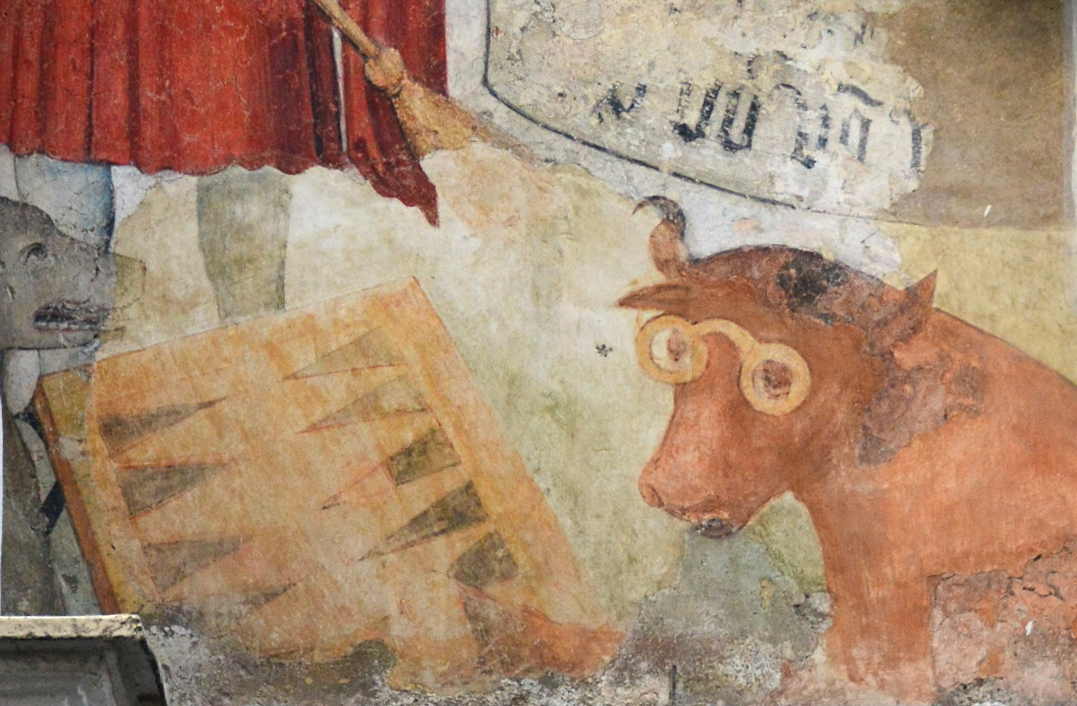
\includegraphics[width=85truemm]{slike/01_Dunaj.jpg}
\caption{Freska na Dunaju (17. stoletje) prikazuje kravo z očali.}
\label{fig:01_Dunaj}
\end{figure}

Odgovore na vprašanja, kako deluje leča in zakaj očala izboljšajo vid, je podal
Kepler\footnote{~Nemški astronom Johannes Kepler, 1571--1630.} leta 1611. 
Poleg tega je odkril totalni odboj svetlobe in zapisal lomni zakon za majhne kote.
Na splošno je začetek sedemnajstega stoletja predstavljal preporod optike. 
V tem času so na Nizozemskem začeli izdelovati prve daljnoglede oziroma
teleskope, sestavljene iz dveh leč:
najprej zbiralne in razpršilne, pozneje pa iz dveh zbiralnih leč. 
Nizozemski znanstvenik Snell\footnote{~Nizozemski matematik in astronom Willebrord 
Snell van Royen, 1580--1626.} je zapisal lomni zakon v današnji obliki in 
marsikje zato lomni zakon še vedno imenujejo po njem. Pomemben teorem, s katerim
bomo tudi mi začeli obravnavno optike v naslednjem poglavju, je postavil 
Fermat\footnote{~Francoski pravnik in matematik Pierre de Fermat, 1601--1665.} 
leta 1657. Teorem pravi, da svetloba med dvema točkama potuje po tisti poti, 
po kateri do cilja pride najhitreje.

V drugi polovici sedemnajstega stoletja so Grimaldi\footnote{~Italijanski 
fizik in astronom Francesco Maria Grimaldi, 1618--1663.}, Huygens\footnote{~Nizozemski 
astronom in matematik Christiaan Huygens, 1629--1695.} in Hooke\footnote{~Angleški 
fizik in zdravnik Robert Hooke, 1635--1703.} proučevali uklon. Ugotovili so, da se 
svetoba širi tudi v območje sence in da torej svetloba ne potuje vedno 
povsem naravnost. Predvsem Huygens je, po podobnosti z zvokom, verjel v 
valovno naravo svetlobe. Širjenje svetlobe je pojasnil z načelom, 
po katerem vsako točko, na katero vpade valovna motnja, obravnavamo 
kot nov točkast izvor, iz katerega se motnja širi v obliki krogelnih valov. 
S tem pristopom je lahko pojasnil odboj in lom na meji dveh sredstev. Sklepal je, da
se svetloba v gostejših snoveh upočasni.
Opazoval in pojasnil je razklon svetlobe na dva žarka v kristalu kalcita 
in s tem odkril polarizacijo svetlobe. Huygens je sodeloval tudi pri 
prvih meritvah hitrosti svetlobe. 

Že od antičnih časov so vedeli, da
je hitrost svetlobe ali zelo velika ali celo neskončna. Prve uspešne kvantitativne
meritve je naredil R\o{}mer\footnote{~Danski astronom
Ole Christensen R\o{}mer, 1644--1710.} leta 1676, ko je z natančnim opazovanjem 
mrkov Jupitrovih lun ugotovil, da je hitrost svetlobe končna. Hitrost svetlobe je
ocenil na $230\,\,000~\si{km/s}$.

K razumevanju svetlobe je pomembno prispeval Newton\footnote{~Angleški 
fizik in matematik Sir Isaac Newton, 1643--1727.}, ko je v letih 1666--72 
izvajal poskuse s stekleno prizmo. S prizmo je razklonil sončno svetlobo v
mavrico in s tem pokazal, da je bela svetloba sestavljena 
iz svetlob različnih barv. Na splošno je bil pristaš teorije, da je 
svetloba sestavljena iz delcev. Ker je bil v tistih časih 
Newton nesporna avtoriteta na področju fizike, je ta pogled obveljal.
\begin{figure}[ht]
\centering
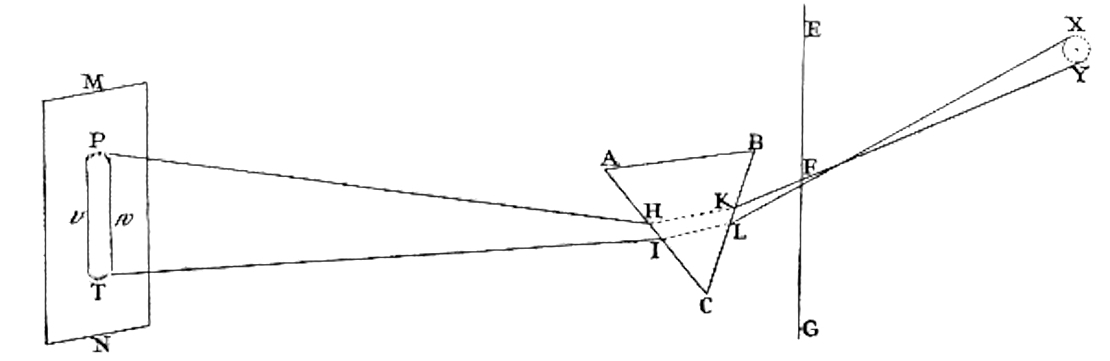
\includegraphics[width=10truecm]{slike/01_Newton.jpg}
\caption{Slika v Newtonovi {\it Optiki} prikazuje razklon sončne svetlobe. Newton 
zapiše, da je razklonjena slika na zaslonu rdeča pri koncu $T$, vijolična
pri koncu $P$, vmes pa rumena, zelena in modra. Vir: https://www.gutenberg.org/}
\label{fig:01_Newton}
\vglue-5truemm
\end{figure}

Pristaš valovnega opisa svetlobe je bil med drugimi Euler\footnote{~Švicarski 
matematik in fizik Leonhard Paul Euler, 1707--1783.}, ki je podal tezo, 
da valovna dolžina valovanja svetlobi določa barvo.
Ključna dognanja za potrditev valovne teorije je leta 1801 prispeval 
Young\footnote{~Angleški zdravnik in fizik Thomas Young, 1773--1829.}, 
ko je z interferenčnimi poskusi precej natančno izmeril valovno dolžino 
vidne svetlobe. Na podlagi Huygensovega valovnega pristopa je 
Fresnel\footnote{~Francoski fizik Augustin Jean Fresnel, 1788--1827.}
leta 1818 pojasnil interferenčne pojave in izračunal vrsto 
uklonskih slik. Z Aragojem\footnote{~Francoski astronom in fizik
Fran\c{c}ois Jean Dominique Arago, 1786--1853.} sta proučevala 
dvolomnost kristalov in interferenco različno odklonjenih žarkov. 
Opazila sta, da med dvema različno polariziranima valovanjema ne 
pride do interference. To je porušilo njuno prepričanje v valovno 
naravo svetlobe, saj so do takrat verjeli, da je svetloba
longitudinalno valovanje. Kar nekaj časa je minilo, preden je Young 
rešil problem s predlogom, da je svetloba transverzalno valovanje.
Kmalu za tem je Fresnel zapisal znane enačbe za jakosti odbitega 
in prepuščenga žarka ob vpadu na mejo med dvema sredstvoma.
Fresnel je v poznejših letih proučeval tudi disperzijo svetlobe.

Okoli 1850 sta se najprej Fizeau\footnote{~Francoski fizik Armand Hippolyte
Louis Fizeau, 1819--1896.} in pozneje Foucault\footnote{~Francoski fizik
Jean Bernard L\'{e}on Foucault, 1819--1868} lotila natančnega
merjenja hitrosti svetlobe. Prvi je uporabil vrteče nazobčeno kolo 
in več kot $8~\si{\kilo\meter}$ oddaljeno zrcalo. Z močnim svetilom je posvetil med
zobmi kolesa in opazoval svetlobo, ki se je odbila od 
zrcala.\footnote{~Glej npr. Strnad, {\it Fizika, drugi del}, 
DMFA-založništvo (2018).} Opazil je, da se pri določenih kotnih hitrostih 
vrtenja kolesa odbita svetloba ne vrne v izhodišče, saj zadane zob kolesa. 
Na ta način je hitrost svetlobe ocenil na $315\,\,300~\si{km/s}$. Do podobne
vrednosti je prišel tudi Foucault, ki je uporabil eno vrtljivo in eno oddaljeno 
zrcalo. To so bile prve meritve hitrosti svetlobe na Zemlji, zaradi česar
je eksperimentalna postavitev omogočala tudi meritev 
svetlobne hitrosti v snovi. Foucault je leta 1850 nedvomno pokazal, 
da je hitrost svetlobe v snovi manjša od hitrosti svetlobe v zraku, kar je dodatno
potrdilo valovno sliko svetlobe. 

Vzporedno z napredkom optike se je razvijalo tudi področje
elektomagnetizma. Faraday\footnote{~Angleški fizik in kemik Michael Faraday, 1791--1867.} 
je leta 1845 ugotovil, da lahko z močnim magnetnim poljem spreminja
smer polarizacije žarka svetlobe. Verjetno najpomembnejše delo
na tem področju je prispeval Maxwell\footnote{~Škotski fizik James Clerk Maxwell, 
1831--1879.}, ki je v sedemdesetih letih devetnajstega stoletja
zbral in dopolnil znanje o elektromagnetizmu in zapisal enačbe, ki jih 
danes imenujemo po njem. Na podlagi teh enačb je povsem 
teoretično pokazal, da je splošno elektromagnetno valovanje 
transverzalno. Izračunal je njegovo hitrost in jo
izrazil le s fizikalnimi konstantami. Presenetljivo se je izračunana 
hitrost elektromagnetnega valovanja ujemala 
z izmerjeno hitrostjo svetlobe, zato je Maxwell sklepal, da je svetloba 
elektromagnetno valovanje. Eksperimentalno potrditev je leta
1888 ponudil Hertz\footnote{~Nemški fizik 
Heinrich Rudolf Hertz, 1857--1894.} z lomom in odbojem elektromagnetnih 
valov. Takrat ni bilo več dvoma -- svetloba je transverzalno 
elektromagnetno valovanje. 

Odprto je ostalo vprašanje, ali svetloba za svoje širjenje 
potrebuje snov, tako imenovani eter. Z vprašanjem etra se je 
ukvarjalo veliko raziskovalcev, med drugim Arago, Fresnel, Fizeau, 
Airy\footnote{~Angleški astronom in matematik Sir George Biddell Airy, 1801--1892.} 
in Lorentz\footnote{~Nizozemski fizik in nobelovec Hendrik Antoon Lorentz, 1863--1928.},
vendar je dokončen odgovor podal šele Michelson\footnote{~Ameriški fizik in nobelovec Albert
Abraham Michelson, 1852--1931.} s svojim 
interferenčnim poskusom v letih 1881 in 1887. Pokazal je, da
sta hitrosti svetlobe enaki v smeri gibanja Zemlje po prostoru in 
pravokotno nanjo. S tem je dokončno ovrgel obstoj etra in pokazal, 
da elektromagnetno valovanje za širjenje ne potrebuje snovi. 
Einstein\footnote{~Nemški fizik in nobelovec Albert Einstein, 1879--1955.} 
je naredil še korak dlje in trdil, da je hitrost 
svetlobe neodvisna od gibanja opazovalca, s čimer je postavil temelje 
teoriji relativnosti. Po dogovoru iz leta 1983 je danes 
hitrost svetlobe  definirana kot $299\,\,792\,\,458~\si{m/s}$. 

Vrnimo se še enkrat v dvajseta leta devetnajstega stoletja, ko je 
Fraunhofer\footnote{~Nemški fizik Joseph von Fraunhofer, 1787--1826.}
proučeval razklon svetlobe na prizmah in uklonskih mrežicah. Izredno
natančna izdelava kakovostnih optičnih naprav mu je najprej omogočila odkritje 
natrijevega dubleta, nato pa opazovanje manjkajočih črt v spektru
svetlobe s Sonca. Pol stoletja je trajalo, da
sta Bunsen\footnote{~Nemški kemik Robert Wilhelm Eberhard Bunsen, 1811--1899.}
in Kirchhoff\footnote{~Nemški fizik Gustav Robert Kirchhoff, 1824--1887.}
pojasnila temne črte v spektru z absorpcijo v snovi in postavila temelje
moderne spektroskopije.

Na podlagi Kirchhoffovega dela je Planck\footnote{~Nemški fizik in nobelovec
Max Karl Ernst Ludwig Planck, 1858--1918.} ob prelomu stoletja
proučeval sevanje črnega telesa. Po več poskusih, ki se niso
ujemali z eksperimentalnimi opažanji, je predlagal povsem novo rešitev problema
v obliki kvantizirane energije elektromagnetnega polja. Na osnovi
Planckove teorije je Einstein oživel delčni model svetlobe, pri čemer
je privzel, da je svetloba sestavljena iz kvantov energije, kasneje 
poimenovanih fotoni. Z Einsteinovo razlago fotoefekta je bila dokončno
potrjena kvantna narava svetlobe. Danes svetlobo obravnavamo
dualno: kot valovanje, ki pojasni interferenčne 
pojave, in hkrat kot delce, ki pojasnijo fotoefekt. 

\chapterimage{02_Geometrijska.jpg} % Chapter heading image

\chapter{Geometrijska optika}
V tem poglavju bomo na kratko predstavili geometrijsko optiko,
v kateri svetlobo obravnavamo kot ravne žarke. Zapisali bomo
žarkovno enačbo, vpeljali matrike ABCD za račun prehoda svetlobe
skozi optične elemente in na
primerih pokazali njihovo uporabo. Na koncu bomo opisali 
delovanje nekaterih preprostih optičnih naprav. 

\section{Fermatov teorem in optična pot}
V uvodnem zgodovinskem pregledu smo zapisali Fermatov teorem, 
ki pravi, da svetloba med dvema točkama potuje po tisti poti, 
za katero potrebuje najmanj časa. Označimo
hitrost svetlobe v snovi s $c$ in na splošno se  $c$ razlikuje
od hitrosti svetlobe v praznem prostoru $c_0$. Razmerje med
hitrostjo svetlobe v praznem prostoru in njeno hitrostjo
v snovi opisuje lomni količnik $n$. Velja:\index{Hitrost svetlobe}
\boxeq{eq:c}{
c = \frac{c_0}{n}.
}
Hitrost svetlobe v praznem prostoru je
po definiciji enaka $c_0 = 299\,\,792\,\,458~\si{m/s}$, 
lomni količnik pa je odvisen od snovi in frekvence svetlobe: za vidno svetlobo
je v vodi približno $1,3$, v steklih okoli $1,4$--$1,9$ in v diamantu $2,4$.\index{Lomni količnik}

Naj svetloba potuje po snovi z lomnim količnikom $n$. Celotno pot, ki 
jo svetloba opravi od začetne do končne točke, razdelimo na kratke intervale 
poti $ds$. Za del poti $ds$ potrebuje svetloba čas $dt$, ki ga zapišemo kot:
\begin{equation}
 dt = \frac{ds}{c} = \frac{ds}{c_0/n} = \frac{nds}{c_0}.
\label{eq:02_02}
\end{equation}
Fermatov teorem pravi, \index{Fermatov teorem}da svetloba od točke 1 do točke 2 potuje po poti, za katero velja:
\beq
\int_1^2 dt = \int_1^2 \frac{nds}{c_0} = \mathrm{min}.
\label{eq:02_03}
\eeq
Če je lomni količnik konstanten, svetloba potuje naravnost in 
ne spreminja smeri. Na splošno pa se lomni količnik spreminja s 
krajem, zato teorem prepišemo v:
\boxeq{eq:02_04}{
S = \int_1^2 n(\mathbf{r})ds = \mathrm{min}.
}
Celotni integral $S$ imenujemo optična pot, ki se od geometrijske poti razlikuje v tem,
da upošteva tudi lomni količnik snovi.\index{Optična pot} 
Zapisani izraz imenujemo princip najmanjše optične poti oziroma najmanjše optične akcije. 
Problem je podoben principu najmanjše akcije v klasični mehaniki, zato včasih govorimo  
tudi o Lagrangeevi oziroma Hamiltonovi optiki.
\begin{remark}
Princip najkrajše optične poti lahko formalno izpeljemo z 
obravnavo valovnih front in žarkov v valovni optiki, če naredimo limito $\lambda \to 0$.
Tako lahko izhajajoč iz Maxwellovih enačb pokažemo pravilnost Fermatovega teorema.
\end{remark}

\begin{example}
{\bf Izpeljava lomnega zakona iz Fermatovega teorema.}
Naj svetlobni žarek vpada na ravno mejo med dvema snovema. Levo od meje je snov 
z lomnim količnikom $n_1$, desno pa snov z lomnim količnikom $n_2$. Svetloba 
potuje od točke 1, ki jo izberemo na oddaljenosti $z_1$ levo 
od meje, do točke 2 na oddaljenosti $z_2$ desno od meje. Vzdolžno razdaljo med obema
točkama označimo z $x$ (slika~\ref{fig:02_FerLom}). 
\begin{figure}[ht]
\centering
\def\svgwidth{100truemm} 
\input{slike/02_FerLom.pdf_tex}
\caption{K izračunu loma na meji dveh snovi}
\label{fig:02_FerLom}
\end{figure}

Naša naloga je poiskati pot žarka svetlobe od točke 1 do točke 2 ob pogoju, 
da je skupna optična pot najkrajša.
Celotno optično pot zapišemo kot:
\begin{equation}
S = n_1 s_1 + n_2 s_2 = n_1 \sqrt{x_1^2+z_1^2}\, +\, n_2 \sqrt{x_2^2+z_2^2}.
\label{eq:02_05}
\end{equation}
Parameter $x_2$ izrazimo z lego iskane točke $x_1$ in dobimo: 
\begin{equation}
S = n_1 \sqrt{x_1^2+z_1^2}\, +\, n_2 \sqrt{(x-x_1)^2+z_2^2}.
\label{eq:02_06}
\end{equation}
Najkrajšo optično pot izračunamo tako, da poiščemo vrednost $x_1$, 
pri kateri je odvod optične poti po $x_1$ enak nič. Izračunamo odvod in zapišemo:
\begin{equation}
\frac{dS}{dx_1} = \frac{2 n_1 x_1}{2 \sqrt{x_1^2+z_1^2}}+
\frac{-2n_2 (x-x_1)}{2 \sqrt{(x-x_1)^2+z_2^2}} = 0.
\label{eq:02_07}
\end{equation}
Vpeljemo vpadni kot $\alpha$ glede na \index{Vpadni kot}normalo na mejo med snovema (slika~\ref{fig:02_FerLom}):
\begin{equation}
\sin \alpha = \frac{x_1}{\sqrt{x_1^2+z_1^2}}.
\label{eq:02_08}
\end{equation}
Lomni kot $\beta$ naj bo kot med\index{Lomni kot} smerjo žarka v drugi snovi in normalo na mejo med snovema: 
\begin{equation}
\sin \beta = \frac{x_2}{\sqrt{x_2^2+z_2^2}} = \frac{(x-x_1)}{\sqrt{(x-x_1)^2+z_2^2}}.
\label{eq:02_09}
\end{equation}
Vstavimo enačbi~(\ref{eq:02_08}) in (\ref{eq:02_09}) v enačbo~(\ref{eq:02_07})
in dobimo lomni zakon v znani obliki:\index{Lomni zakon}
\boxeq{eq:lomnizakon}{
n_1 \sin \alpha = n_2 \sin \beta.
}
Na podoben način izpeljemo tudi odbojni zakon, \index{Odbojni zakon}tako da izračunamo 
najkrajšo optično pot med točkama 1 in 3. Dobimo:
\boxeq{eq:odbojnizakon}{
\tilde{\alpha} = \alpha.
}
\end{example}

\section{Žarkovna enačba}
\label{chap:zarkovna}
Poglejmo, kako izračunamo najkrajšo optično pot v primeru, ko 
meja med dvema snovema ni ostra, ampak se lomni količnik zvezno spreminja. 
Naj bo lomni količnik v splošnem funkcija kraja: $n = n(\mathbf{r}) = n(x,y,z)$.
Numerično se naloge lotimo tako, da snov razdelimo
na kratke odseke in na mejah med njimi uporabimo lomni ali odbojni zakon.
Analitično problem rešujemo z uporabo Euler-Lagrangeeve enačbe za minimum
funkcionala optične poti $S$:\index{Euler-Lagrangeeva enačba}\index{Optična pot}
\begin{equation}
 S = \int_1^2 n(x,y,z) ds  = \int_1^2 n(x,y,z)\,|\mathbf{v}|\,dt  = 
 \int_1^2 n(x,y,z) \sqrt{\dot{x}^2+ \dot{y}^2+\dot{z}^2} dt,
 \label{eq:02_10}
\end{equation}
pri čemer pika označuje odvod posamezne koordinate po času. Integrand
enačbe predstavlja Lagrangian $L$, ki je funkcija treh koordinat in njihovih
odvodov.\index{Lagrangian}
\begin{equation}
L(x, y, z, \dot{x}, \dot{y}, \dot{z}) = n(x,y,z) \sqrt{\dot{x}^2+ \dot{y}^2+\dot{z}^2}.
\label{eq:02_11}
\end{equation}
Euler-Lagrangeeva enačba\footnote{~Glej npr. P. Prelovšek, {\it Klasična
mehanika}, skripta, 2013.} za koordinato $x$ je oblike:
\begin{equation}
 \frac{d}{dt}\left(\frac{\partial L}{\partial \dot{x}}\right) - 
 \frac{\partial L}{\partial x} = 0.
 \label{eq:02_12}
\end{equation}
Vstavimo Lagrangian (enačba~\ref{eq:02_11}) 
v enačbo~(\ref{eq:02_12}) in dobimo:
\begin{equation}
\frac{d}{dt}\left(n \frac{\dot{x}}{\sqrt{\dot{x}^2+ \dot{y}^2+\dot{z}^2}} \right)
 = \frac{\partial n}{\partial x}\sqrt{\dot{x}^2+ \dot{y}^2+\dot{z}^2}.
  \label{eq:02_13}
\end{equation}
Pomnožimo enačbo z $dt/ds$:
\begin{equation}
\frac{d}{dt}\left(n \frac{\dot{x}}{\sqrt{\dot{x}^2+ \dot{y}^2+\dot{z}^2}} \right)
\frac{dt}{ds}
 = \frac{\partial n}{\partial x}\frac{\sqrt{\dot{x}^2+ \dot{y}^2+\dot{z}^2}\,dt}{ds}.
  \label{eq:02_14}
\end{equation}
Na desni strani enačbe uporabimo zvezo:
\begin{equation}
 \sqrt{\dot{x}^2+ \dot{y}^2+\dot{z}^2} dt = ds,
 \label{eq:02_15}
\end{equation}
na levi strani pa verižno pravilo odvajanja, po katerem lahko pokrajšamo $dt$. Dobimo:
\begin{equation}
 \frac{d}{ds} \left( n \frac{dx}{dt\sqrt{\dot{x}^2+ \dot{y}^2+\dot{z}^2}} \right)=
 \frac{\partial n}{\partial x}.
 \label{eq:02_16}
\end{equation}
Zvezo~(\ref{eq:02_15}) uporabimo še enkrat v oklepaju na levi strani. Sledi:
\begin{equation}
 \frac{d}{ds} \left( n\, \frac{dx}{ds} \right)=
 \frac{\partial n}{\partial x}.
  \label{eq:02_17}
\end{equation}
Podobni enačbi zapišemo še za koordinati $y$ in $z$, nato vse tri enačbe
združimo v enotno žarkovno enačbo:\index{Žarkovna enačba}
\boxeq{eq:zarkovnaenacba}{
\nabla n = \frac{d}{ds} \left( n \frac{d\mathbf{r}}{ds}\right)\!.
}
Rešitev žarkovne enačbe poda trajektorijo optičnega žarka v parametrični 
obliki $\mathbf{r}(s)$. Z uporabo zveze $ds = dz (1+(dx/dz)^2+(dy/dz)^2)^{1/2}$
lahko enačbo prevedemo na sistem diferencialnih enačb za $x(z)$ in $y(z)$. Reševanje
tega sistema enačb je na splošno zelo zapleteno.

\begin{example}
{\bf Žarkovna enačba v homogeni snovi.} Naj svetloba potuje po snovi,
v kateri je lomni količnik konstanten. Potem je $\nabla n = 0$ in 
\begin{equation}
0 = \frac{d}{ds}\left( n \frac{d\mathbf{r}}{ds} \right) = 
n \frac{d^2 \mathbf{r}}{ds^2}.
 \label{eq:02_18}
\end{equation}
Rešitev te enačbe je ravni žarek:
\begin{equation}
 \mathbf{r} = \mathbf{a}_0+\mathbf{a}_1\,s,
  \label{eq:02_19}
\end{equation}
pri čemer vektor $\mathbf{a}_0$ opisuje lego začetne točke, 
vektor $\mathbf{a}_1$ pa ima smer od začetne do končne točke.
\end{example}

\subsection*{Obosni približek žarkovne enačbe}
V optiki pogosto privzamemo, da smer širjenja svetlobe le malo 
odstopa od neke dane smeri. Naj bo to smer $z$, ki jo imenujemo
optična os sistema. \index{Optična os sistema}
Zaradi enostavnosti se omejimo na ravninski primer, 
tako da trajektorijo žarka opazujemo v ravnini $xz$ 
(slika~\ref{fig:02_FerOs}). Lomni količnik naj bo funkcija $n= n(x)$.
\begin{figure}[ht]
\centering
\def\svgwidth{90truemm} 
\input{slike/02_FerOs.pdf_tex}
\caption{K zapisu žarkovne enačbe v obosnem približku. Lomni količnik $n$ se na splošno
spreminja z oddaljenostjo $x$ od optične osi sistema (os $z$).}
\label{fig:02_FerOs}
\end{figure}

Predpostavko, da se žarek širi pretežno v smeri $z$ in od te smeri 
le malo odstopa, matematično zapišemo s pogojem:
\begin{equation}
 \frac{dx}{dz}\ll 1.
  \label{eq:02_20}
\end{equation}
Iz tega sledi, da za naklon žarka $\vartheta$, ki ga na danem mestu izračunamo kot:
\begin{equation}
\vartheta = \frac{dx}{dz},
 \label{eq:02_21}
\end{equation}
velja $\sin \vartheta \approx \tan \vartheta \approx \vartheta \ll 1$.
Upoštevajoč enačbo~(\ref{eq:02_20}) zapišemo:
\begin{equation}
ds = \sqrt{dx^2+dz^2} = \sqrt{1+\left(\frac{dx}{dz}\right)^2}\,\,dz \approx dz.
\label{eq:02_22}
\end{equation}
Predpostavki, da se žarek širi približno vzdolž osi $z$, pravimo\index{Obosni približek}
\index{Paraksialni približek|see{Obosni približek}}
obosni ali paraksialni približek. V nadaljevanju se ga bomo še velikokrat 
posluževali. Žarkovno enačbo (enačba~\ref{eq:zarkovnaenacba}) v obosnem 
približku\index{Žarkovna enačba!Obosni približek|see{Obosni približek}}
zapišemo kot:
\begin{equation}
 \frac{dn}{dx} = \frac{d}{dz}\left(n(x)\,\frac{dx}{dz}\right) = n(x)\,\frac{d^2x}{dz^2}
  \label{eq:02_23}
\end{equation}
oziroma
\boxeq{eq:02_24}{
\frac{d^2x}{dz^2} = \frac{1}{n(x)} \frac{dn}{dx}.
}

\begin{example}
{\bf Žarkovna enačba v snovi s paraboličnim profilom
lomnega količnika.} Izračunajmo trajektorijo žarka svetlobe v 
obosnem približku v snovi, v kateri se lomni količnik parabolično 
spreminja z oddaljenostjo od osi $z$.  Odvisnost lomnega količnika 
od oddaljenosti $x$ od osi $z$ zapišemo kot:
\begin{equation}
 n(x) = n_0 \left(1-\frac{\alpha^2\,x^2}{2}\right)\!,
 \label{eq:02_25}
\end{equation}
pri čemer je $\alpha x \ll 1$.
Vstavimo izraz za lomni količnik (enačba~\ref{eq:02_25}) v obosni približek
žarkovne enačbe (enačba~\ref{eq:02_24}) in dobimo:
\begin{equation}
 \frac{d^2x}{dz^2}= \frac{1}{n(x)}\frac{dn}{dx} = 
 \frac{-n_0 \alpha^2x}{n_0 \left(1-\alpha^2\,x^2/2\right)} 
 \approx -\frac{n_0\alpha^2x}{n_0} = -\alpha^2x.
 \label{eq:02_26}
\end{equation}
Enačbo~(\ref{eq:02_26}) preprosto rešimo in dobimo splošno 
obliko trajektorije:
\begin{equation}
 x(z) = A \cos (\alpha z) + B \sin (\alpha z).
  \label{eq:02_27}
\end{equation}
Naj bo v izhodišču pri $z=0$ žarek na oddaljenosti $x_0$ 
in naj se širi pod kotom $\vartheta_0$. 
Z upoštevanjem začetnih pogojev dobimo rešitev:
\begin{equation}
x (z) = x_0 \cos(\alpha z) + \frac{\vartheta_0}{\alpha} \sin (\alpha z).
 \label{eq:02_28}
\end{equation}
Rešitve obosnega približka žarkovne enačbe v snovi s paraboličnim profilom 
so torej oscilatorne funkcije s periodo $2\pi/\alpha$ (glej sliko~\ref{fig:02_FerPar}).
\begin{figure}[ht]
\centering
\def\svgwidth{100truemm} 
\input{slike/02_FerPar.pdf_tex}
\caption{Rešitev žarkovne enačbe v snovi s paraboličnim profilom lomnega
količnika je periodična. Narisanih
je šest žarkov, pri katerih je $x_0=0$, razlikujejo pa se v $\vartheta_0$.}
\label{fig:02_FerPar}
\end{figure}

\begin{figure}[ht]
\centering
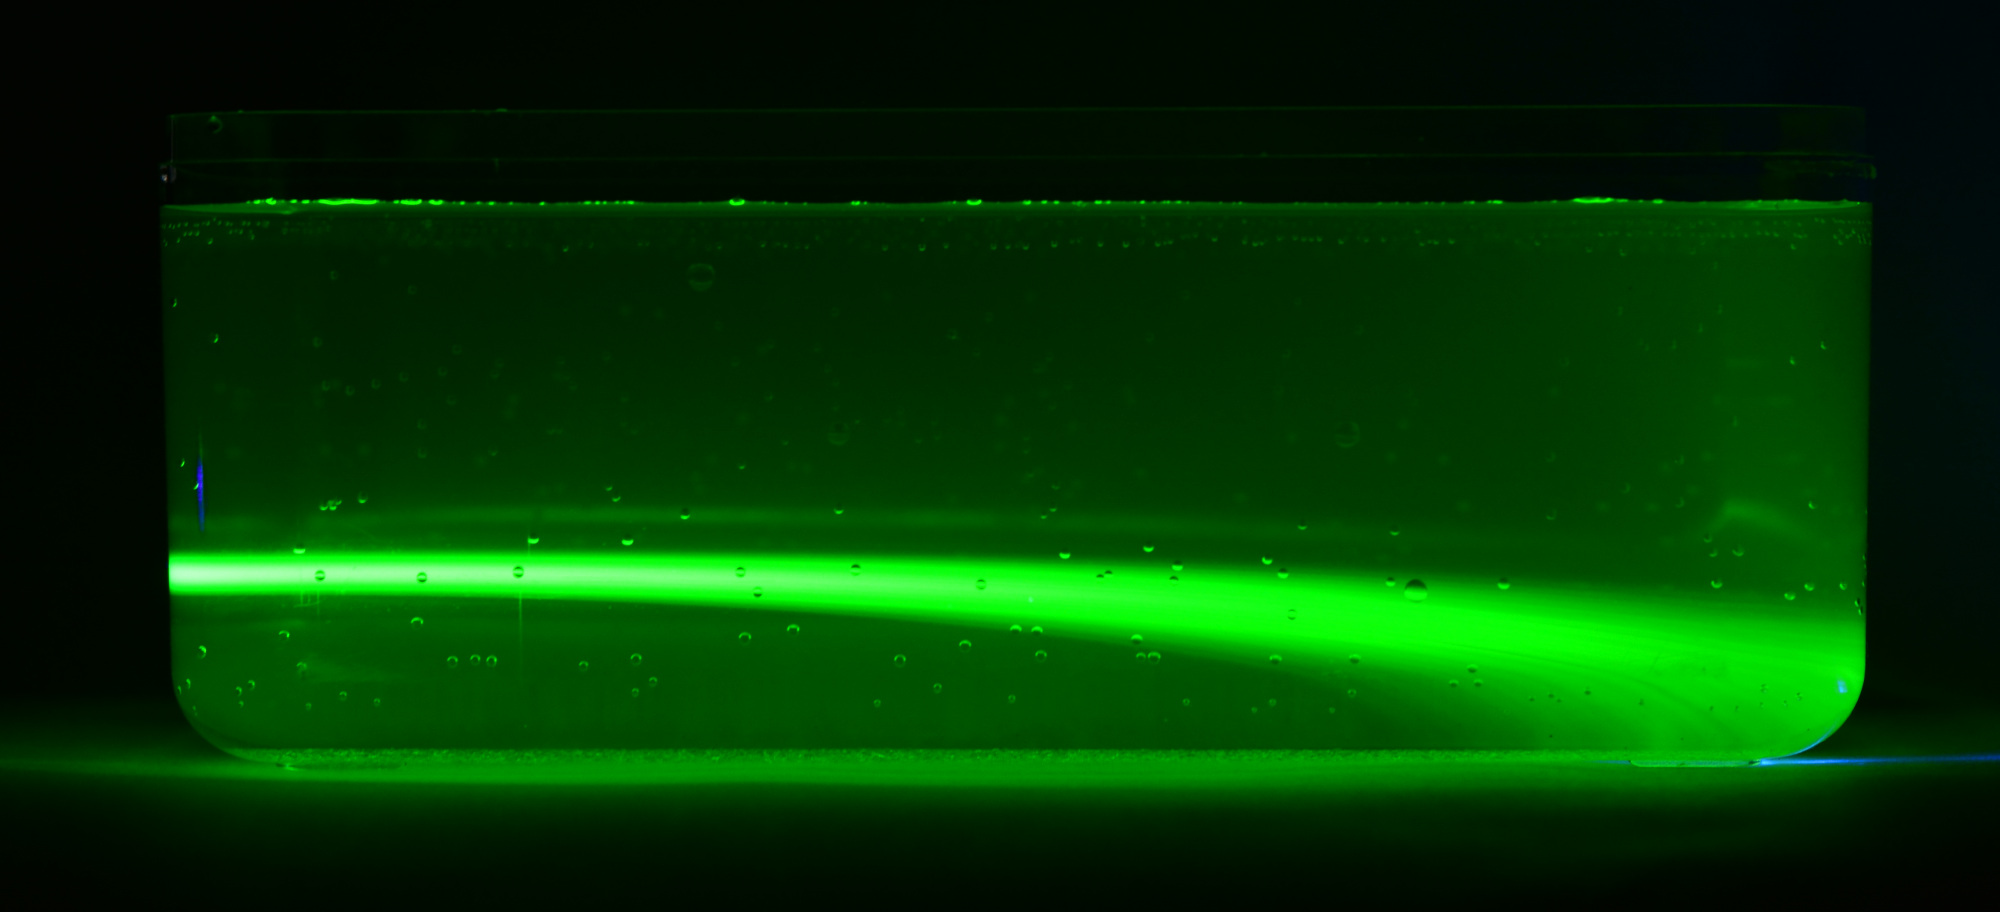
\includegraphics[width=10truecm]{slike/02_Sladkor.jpg}
\caption{Potek žarka v vodni raztopini sladkorja, v kateri koncentracija sladkorja in z
njo lomni količnik naraščata z globino. Vodi smo dodali fluorescein, da bolje vidimo potek žarka. Podobno se ukrivi potek žarka v neenakomerno segreti atmosferi, kar vodi
do pojava fatamorgane.}
\label{fig:02_Sladkor}
\end{figure}
\end{example}

\subsection*{Fatamorgana}\index{Fatamorgana}
Ukrivljeno pot žarkov v snovi z nehomogenim lomnim količnikom opazimo
tudi v naravi. Kadar se tla (na primer asfaltna cesta) 
močno segrejejo, nastane nad njimi tanka plast zraka, ki je bistveno 
toplejši od zraka višje nad tlemi. Ali pa je tanka plast zraka nad 
hladnim morjem znatno hladnejša od toplega zraka v višjih legah. Ker je 
lomni količnik toplejšega zraka manjši od lomnega količnika hladnejšega zraka, 
se v obeh primerih pot svetlobe ukrivi, enkrat navzgor, drugič navzdol. Ta pojav
imenujemo zračno zrcaljenje ali fatamorgana.\index{Zračno zrcaljenje|see{Fatamorgana}}
Spodnje zračno zrcaljenje nastopi, kadar je spodnja plast zraka toplejša 
od zgornjih plasti. Poglejmo, kako opazovalec vidi oddaljeno drevo 
(slika~\ref{fig:02_Fata1}). Od krošnje do opazovalca pridejo žarki
po razmeroma hladni plasti, hkrati pa pridejo do njega tudi žarki, ki 
se ukrivijo na močno segreti plasti zraka tik nad tlemi. Opazovalec
tako vidi dve sliki -- eno pravo in pod njo eno obrnjeno. Na enak način 
pojasnimo tudi odsev neba, ki ga pogosto vidimo na razgretih cestah.
Ker smo vajeni opazovati
odsev neba od vodne gladine, je vroča cesta videti mokra.
\begin{figure}[h!]
\centering
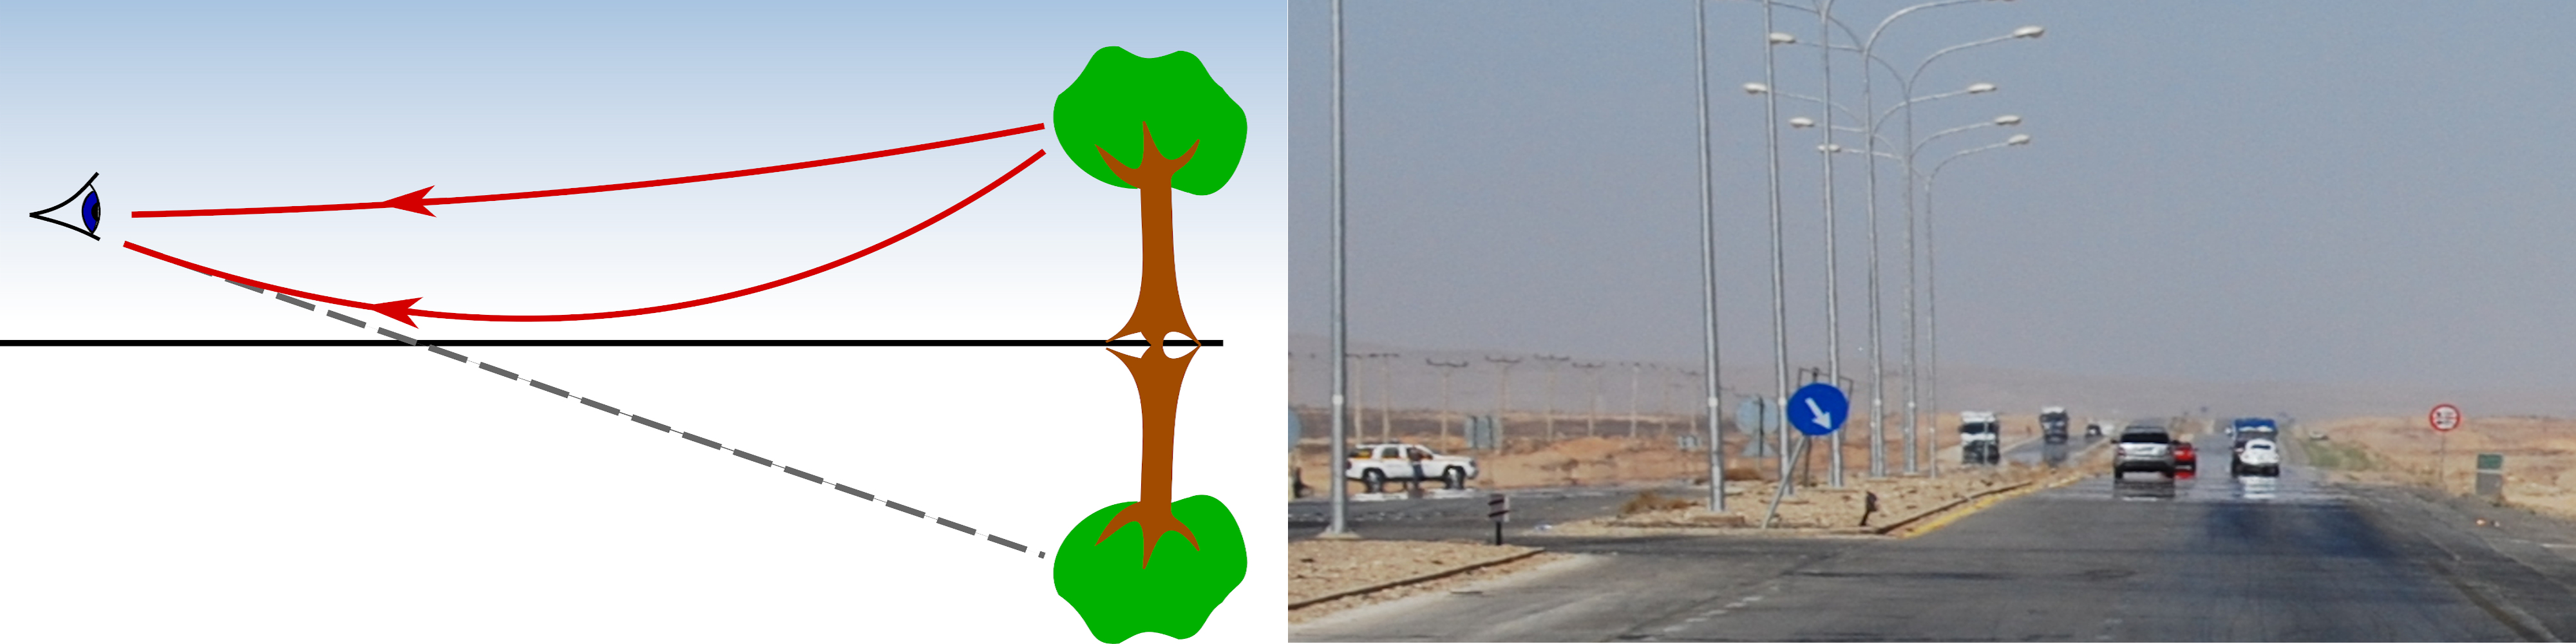
\includegraphics[width=12truecm]{slike/02_Fata1.jpg}
\caption{Zračno zrcaljenje na vročih tleh}
\label{fig:02_Fata1}
\end{figure}
\vglue-0.6truecm
Zgornje zračno zrcaljenje se nasprotno pojavi, 
kadar je spodnja plast zraka izrazito hladnejša od zgornjih plasti. 
Takrat se svetlobni žarki krivijo navzdol (slika~\ref{fig:02_Fata2})
in navidezno sliko predmeta premaknejo nad njegovo dejansko lego. 
Slika je lahko pokončna ali obrnjena, odvisno od oddaljenosti predmeta
in temperature plasti. 
\begin{figure}[h!]
\centering
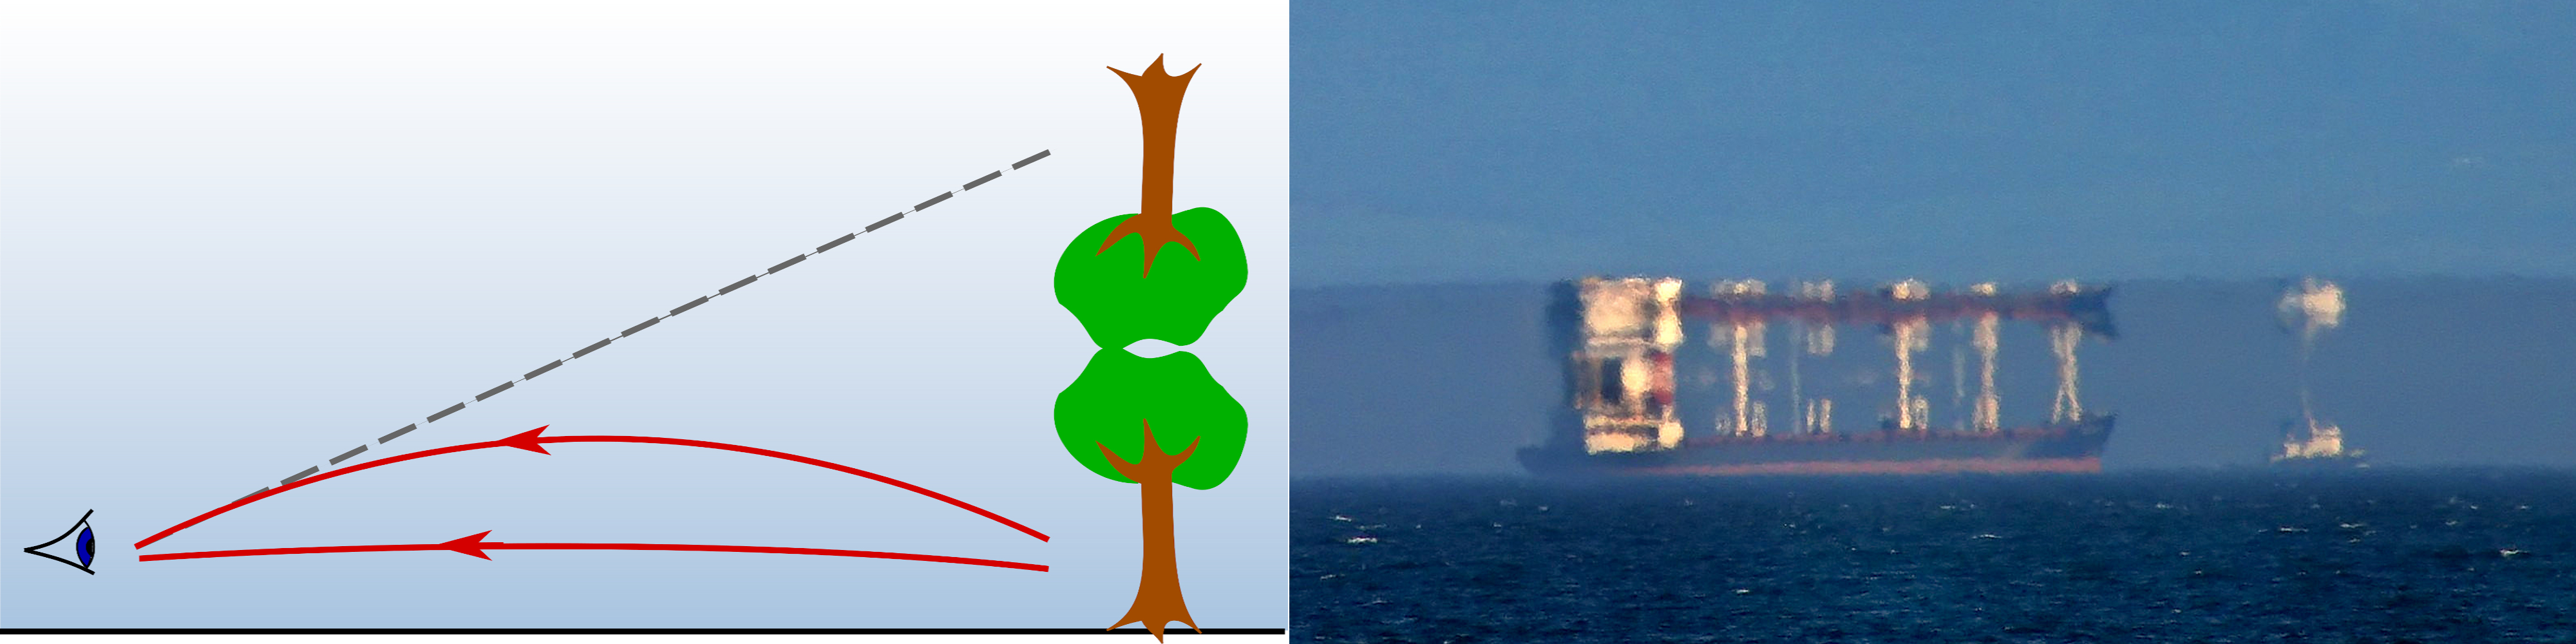
\includegraphics[width=12truecm]{slike/02_Fata2.jpg}
\caption{Zračno zrcaljenje na hladnejši podlagi. Foto: Craig Clements, Wikimedia.}
\label{fig:02_Fata2}
\end{figure}
\vglue-0.6truecm
Ukrivljena pot žarkov zaradi temperaturnega gradienta v atmosferi
vodi še do enega zanimivega pojava: popačenja oblike Sonca ob sončnem 
zahodu. Ker žarki s spodnjega dela Sonca potujejo po bolj ukrivljeni\index{Sonce}
poti kot žarki z zgornjega dela, se spodnji rob navidezno premakne navzgor 
in slika Sonca se splošči ali popači (slika~\ref{fig:02_Sonce}).
\begin{figure}[ht]
\centering
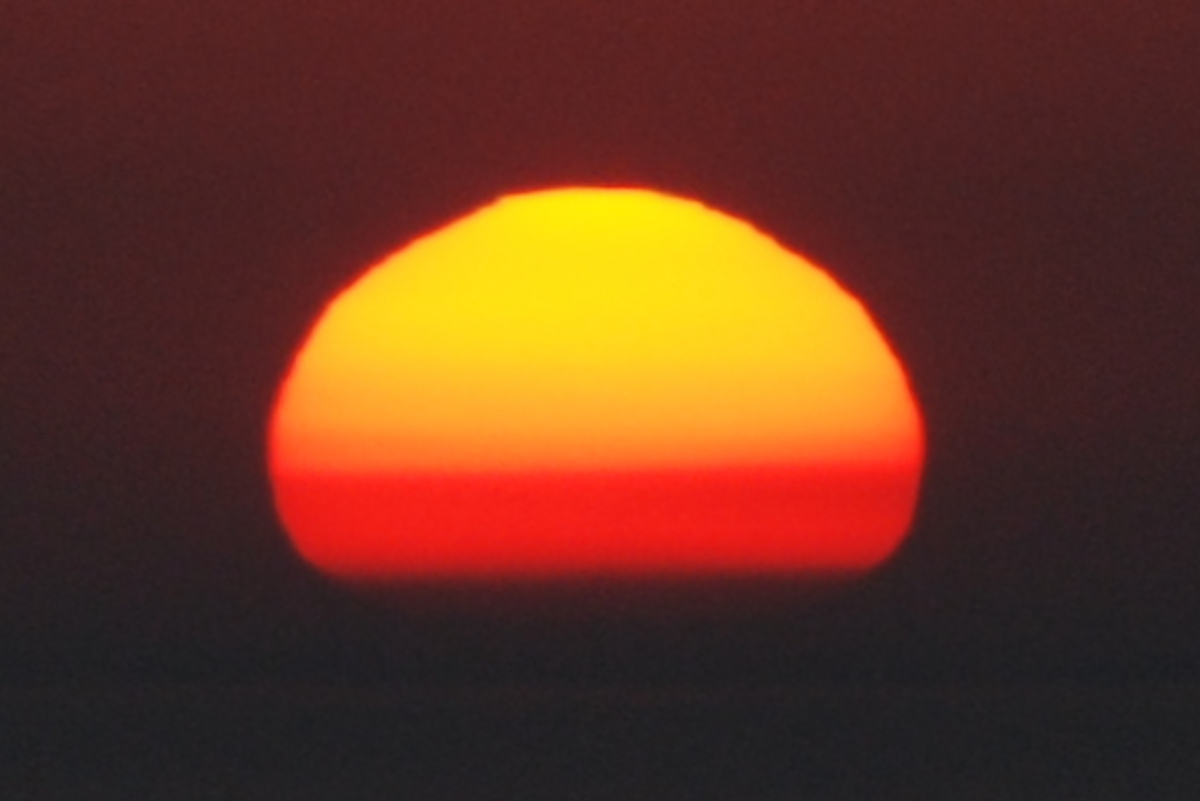
\includegraphics[width=5truecm]{slike/02_Sonce.jpg}
\caption{Sonce se ob sončnem zahodu navidezno splošči in njegova oblika popači.}
\label{fig:02_Sonce}
\end{figure}
\vglue-0.6truecm
\section{Transformacije žarkov z matrikami ABCD}
V prejšnjem razdelku smo zapisali žarkovno enačbo v obosnem 
približku (enačba~\ref{eq:02_24}). Ključna parametra za opis trajektorije žarka sta 
oddaljenost od optične osi $z$, ki jo označimo z $x$, in naklonski 
kot žarka glede na optično os, ki ga označimo s $\vartheta$ (slika~\ref{fig:01_ABCD0}).
Naša naloga je povezati dve točki žarka na različnih mestih v
prostoru in zapisati preslikavo med njima, če je med točkama
optični medij oziroma nek optični element. 
\begin{figure}[ht]
\centering
\def\svgwidth{90truemm} 
\input{slike/02_ABCD0.pdf_tex}
\caption{Pri danem $z$ žarek opišemo z lego $x$ in smerjo $\vartheta$. Spremembo
teh dveh parametrov opišemo s preslikavo.}
\label{fig:01_ABCD0}
\end{figure}

Na splošno vrednosti lege in naklona v točki 2 izrazimo kot 
linearno kombinacijo prvotnih vrednosti v točki 1:
\begin{align}
 x_2 &= A x_1 + B \vartheta_1 \qquad \mathrm{in}  \label{eq:02_29}\\
 \vartheta_2 &=  C x_1 + D\vartheta_1.
 \label{eq:02_30}
\end{align}
Če združimo parametra $x$ in $\vartheta$ v neki točki prostora
v dvodimenzionalni vektor,
lahko preslikavo strnjeno zapišemo v matrični obliki:
\boxeq{eq:02_31}{
\left[\begin{array}{c}
x_2\\
\vartheta_2
\end{array}\right] = 
\left[\begin{array}{cc}
A& B\\
C&D
\end{array}\right]
\left[\begin{array}{c}
x_1\\
\vartheta_1
\end{array}\right]
= M \left[\begin{array}{c}
x_1\\
\vartheta_1
\end{array}\right]\!\!.
}
Matrika $M$ je  transformacijska oziroma prehodna matrika 
vmesnega optičnega medija ali optičnega elementa. Imenujemo jo matrika ABCD.
\index{Matrika ABCD}

\begin{example}
\label{ex:ML}\index{Matrika ABCD!{pri premiku}}
{\bf Matrika ABCD za premik v homogeni snovi s konstantnim lomnim količnikom.} 
Prvi primer naj bo homogena snov, v kateri je lomni količnik konstanten in enak $n$. 
V točki 1 pri $z_1$ naj bosta komponenti vektorja enaki $x_1$ in 
$\vartheta_1$. Poiščimo vrednosti komponent vektorja pri $z_2$, ki je 
za $L$ premaknjen vzdolž optične osi sistema 
(slika~\ref{fig:01_ABCD1}). 
\begin{figure}[ht]
\centering
\def\svgwidth{70truemm} 
\input{slike/02_ABCD1.pdf_tex}
\caption{K izračunu matrike ABCD za premik v homogeni snovi}
\label{fig:01_ABCD1}
\end{figure}

Naklon žarka se pri premiku ne spremeni, zato ostane $\vartheta_2 = \vartheta_1$. Spremeni
pa se odmik od optične osi, saj žarek ne potuje vzporedno z osjo $z$. 
Vrednost $x_2$ zapišemo kot:
\begin{equation}
 x_2 = x_1 + (z_2-z_1)\vartheta_1 = x_1 + L\vartheta_1.
\label{eq:02_32}
\end{equation}
Potem zapišemo sistem enačb:
\begin{align}
 x_2 &= 1\cdot x_1 + L\cdot \vartheta_1 \qquad \mathrm{in} \label{eq:02_33}\\
 \vartheta_2 &= 0\cdot x_1 + 1\cdot \vartheta_1.
 \label{eq:02_34}
\end{align}
Iz zapisa razberemo koeficiente matrike $M$ za homogeno snov dolžine $L$:
\begin{equation}
 M = \left[\begin{array}{cc}
1& L\\
0&1
\end{array}\right]\!\!.
 \label{eq:02_35}
\end{equation}
\end{example}

\begin{example}
\label{ex:Mmeja}\index{Matrika ABCD!{na ravni meji}}
{\bf Matrika ABCD za prehod skozi ravno mejo med dvema snovema.} Naj svetloba vpada na 
mejo med dvema snovema z različnima lomnima količnikoma $n_1$ in $n_2$ (slika~\ref{fig:01_ABCD2}). Za izračun 
prehodne matrike izberemo dve točki na žarku: eno tik pred mejo in eno tik za njo. 
Lega žarka se ob tem ne spremeni in $x_2 = x_1$. 
Spremeni pa se naklon žarka. 
\begin{figure}[ht]
\centering
\def\svgwidth{70truemm} 
\input{slike/02_ABCD2.pdf_tex}
\caption{K izračunu matrike ABCD za prehod skozi ravno mejo med dvema snovema}
\label{fig:01_ABCD2}
\end{figure}

Za majhne naklone lahko lomni zakon
(enačba~\ref{eq:lomnizakon}) razvijemo in dobimo:
\begin{equation}
n_1 \vartheta_1 = n_2 \vartheta_2.
 \label{eq:02_36}
\end{equation}
Sistem enačb je potem:
\begin{align}
 x_2 &= 1\cdot x_1 + 0\cdot \vartheta_1 \qquad \mathrm{in} \label{eq:02_37}\\
 \vartheta_2 &= 0\cdot x_1 + \frac{n_1}{n_2}\cdot \vartheta_1.
 \label{eq:02_38}
\end{align}
Matrika $M$ za prehod skozi mejo med dvema snovema je:
\begin{equation}
 M = \left[\begin{array}{cc}
1& 0\\
0&\frac{n_1}{n_2}
\end{array}\right]\!\!.
\label{eq:02_39}
\end{equation}
\end{example}

\begin{example}
\label{ex:MUmeja}\index{Matrika ABCD!{na ukrivljeni meji}}
{\bf Matrika ABCD za prehod skozi ukrivljeno mejo med dvema snovema.} 
Poglejmo še matriko za prehod skozi ukrivljeno mejo med snovema z lomnima 
količnikoma $n_1$ in $n_2$. Krivinski radij mejne ploskve
naj bo $R$, pri čemer $R$ štejemo pozitivno, če je meja konveksna glede na smer
naraščajočega $z$ oziroma če je središče krožnice za mejo med snovema. Kadar
je središče krožnice, ki določa mejo med snovema, pred mejo, je meja konkavna, 
krivinski radij mejne ploskve pa negativen. 

Za izračun matrike ponovno izberemo dve točki, prvo tik pred mejo in 
drugo tik za njo. To pomeni, da se oddaljenost od optične osi
pri prehodu ohranja in $x_1 = x_2$. 

Izračun naklona žarka po prehodu je malo bolj zapleten. Za zapis lomnega 
zakona moramo namreč vpeljati kote glede na normalo na
mejo. Vpadni kot je tako $\alpha = \vartheta_1 + \varphi$, lomni kot pa 
$\beta = \vartheta_2 + \varphi$ (glej sliko~\ref{fig:02_ABCD3}).
Privzamemo, da je ukrivljenost meje dovolj majhna oziroma da so žarki
dovolj blizu optične osi, da velja zveza:
\begin{equation}
 \sin \varphi = \frac{x_1}{R} \approx \varphi.
 \label{eq:02_40}
\end{equation}
\begin{figure}[!h]
\centering
\def\svgwidth{70truemm} 
\input{slike/02_ABCD3.pdf_tex}
\caption{K izračunu matrike ABCD za prehod skozi ukrivljeno mejo med dvema snovema}
\label{fig:02_ABCD3}
\end{figure}

Zapišemo lomni zakon,
pri čemer privzamemo, da so vsi koti majhni:
\begin{equation}
n_1 (\vartheta_1 + \varphi) = n_2 (\vartheta_2 + \varphi).
\label{eq:02_41}
\end{equation}
Od tod izračunamo kot $\vartheta_2$:
\begin{equation}
 \vartheta_2 = \frac{n_1-n_2}{n_2}\varphi + \frac{n_1}{n_2} \vartheta_1.
 \label{eq:02_42}
 \end{equation}
Če $\varphi$ izrazimo iz enačbe~(\ref{eq:02_40}), zapišemo transformacijo koordinat:
\begin{align}
 x_2 &= 1\cdot x_1 + 0\cdot \vartheta_1 \qquad \mathrm{in} \\
 \vartheta_2 &= \frac{n_1-n_2}{n_2R}\cdot x_1 + \frac{n_1}{n_2}\cdot \vartheta_1.
 \label{eq:02_43}
\end{align}
Razberemo matriko $M$ za prehod skozi ukrivljeno mejo med dvema snovema:
\begin{equation}
M = \left[\begin{array}{cc}
1& 0\\
\frac{n_1-n_2}{n_2R}&\frac{n_1}{n_2}
\end{array}\right]\!\!.
 \label{eq:02_44}
\end{equation}
V limitnem primeru, ko gre $R \to \infty$, se matrika prevede na matriko za
prehod skozi ravno mejo (glej primer~\ref{ex:Mmeja}).
\end{example}

Izračunajmo še determinanto izpeljanih matrik ABCD. \index{Matrika ABCD!determinanta}Na splošno velja, da
je determinanta matrike ABCD enaka razmerju lomnih količnikov začetne in 
končne snovi. Če je lomni količnik snovi na koncu enak
kot na začetku (primer~\ref{ex:ML}), je $\det(M) = 1$, v nasprotnem primeru 
(primera~\ref{ex:Mmeja} in \ref{ex:MUmeja}) je $\det(M) = n_1/n_2$.

Do zdaj smo obravnavali matrike za posamezne prehode. Poglejmo, kako izračunamo
prehodno matriko za primer, če svetloba potuje skozi več elementov zapored (slika~\ref{fig:01_MMM}). V tem
primeru se pokažeta izjemna praktičnost in uporabnost zapisa z matrikami, saj ob prehodu svetlobe skozi 
več elementov matrike za te elemente preprosto zmnožimo. Paziti moramo seveda
na vrsti red: matriko za element, na katerega vpade svetloba najprej, zapišemo
najbolj desno, to je najbliže vektorju, ki opisuje vpadno svetlobo. Celoten prehod
spet opiše ena sama matrika:\index{Matrika ABCD!množenje}
\begin{equation}
\left[\begin{array}{c}
x_N\\
\vartheta_N
\end{array}\right] 
= \tilde{M} \left[\begin{array}{c}
x_1\\
\vartheta_1
\end{array}\right]\!\!,
 \label{eq:02_45}
\end{equation}
pri čemer je:
\begin{equation}
\tilde{M} = M_N \cdot M_{N-1}~...~M_2 \cdot M_1.
 \label{eq:02_46}
\end{equation}
\begin{figure}[ht]
\centering
\def\svgwidth{100truemm} 
\input{slike/02_MMM.pdf_tex}
\caption{Prehod žarka skozi več optičnih elementov zapišemo kot produkt matrik posameznih prehodov.
Pri tem moramo paziti na vrstni red zapisa matrik.}
\label{fig:01_MMM}
\end{figure}

\section{Preslikave z lečami}
\label{chap:lecje}\index{Leča}
Uporabimo matrike ABCD za izračun prehoda svetlobe skozi tanko lečo. Matriko
za prehod zapišemo kot produkt dveh matrik: prve, ki opiše
prehod skozi prvo ukrivljeno ploskev s krivinskim radijem $R_1$, 
in druge, ki opiše prehod skozi izhodno ukrivljeno ploskev s 
krivinskim radijem $R_2$. Za bikonveksno lečo na sliki~\ref{fig:02_tankaleca} velja 
$R_1>0$ in $R_2<0$.
Lomni količnik leče naj bo $n_2$, lomni količnik snovi okoli leče 
(navadno je to zrak) pa naj bo $n_1$. Zanima nas, kako se vektor $(x_1, \vartheta_1)$ 
preslika v $(x_2, \vartheta_2)$.
\begin{figure}[!h]
\centering
\def\svgwidth{100truemm} 
\input{slike/02_tankaleca.pdf_tex}
\caption{K izračunu matrike ABCD za prehod skozi tanko bikonveksno lečo}
\label{fig:02_tankaleca}
\end{figure}

Izračunajmo najprej matriko za prehod skozi lečo. Ker smo privzeli, da je leča tanka, 
vmesne matrike za premik po steklu ne zapišemo. Z upoštevanjem enačbe~(\ref{eq:02_44})
dobimo:
\beq
 M = \left[\begin{array}{cc}
1& 0\\
\frac{n_2-n_1}{n_1R_2}&\frac{n_2}{n_1}
\end{array}\right]\cdot 
\left[\begin{array}{cc}
1& 0\\
\frac{n_1-n_2}{n_2R_1}&\frac{n_1}{n_2}
\end{array}\right] = 
\left[\begin{array}{cc}
1& 0\\
\frac{n_2-n_1}{n_1}\left(\frac{1}{R_2}-\frac{1}{R_1}\right)&1
\end{array}\right]\!\!.
\label{eq:02_47}
\eeq
Vpeljemo parameter $f$, za katerega velja:
\beq
\frac{1}{f} = -\frac{n_2-n_1}{n_1}\left(\frac{1}{R_2}-\frac{1}{R_1}\right)\!\!.
\label{eq:02_48}
\eeq
Element matrike $C$ je tako enak $-1/f$. Fizikalni pomen tega parametra
bomo kmalu spoznali.\index{Matrika ABCD!{za tanko lečo}}

Uporabimo izračunano matriko za opis prehoda svetlobe skozi lečo. Naj žarek izhaja iz 
predmeta, ki je na oddaljenosti $a$ od leče, opazujemo pa ga na razdalji
$b$ za lečo (slika~\ref{fig:02_tankaleca}). Za celotno pot žarka moramo zmnožiti tri matrike: matriko za 
premik do leče, matriko za prehod skozi lečo in matriko za premik do opazovalca. Pazimo na vrstni red in dobimo:
\beq
M = 
\left[\begin{array}{cc}
1& b\\
0&1
\end{array}\right]\cdot
\left[\begin{array}{cc}
1& 0\\
-\frac{1}{f}&1
\end{array}\right]
\cdot
\left[\begin{array}{cc}
1& a\\
0&1
\end{array}\right]
= 
\left[\begin{array}{cc}
1-\frac{b}{f}& a+b-\frac{ab}{f}\\
-\frac{1}{f}&1-\frac{a}{f}
\end{array}\right]\!\!.
\label{eq:02_49}
\eeq
Najprej poiščimo pomen parametra $f$, ki smo ga vpeljali z enačbo~(\ref{eq:02_48}).
Poglejmo, v kaj se preslikajo žarki, ki na neki oddaljenosti od osi $x_1$ vpadajo na lečo 
vzporedno z optično osjo $z$:
\beq
\left[\begin{array}{c}
x_2\\
\vartheta_2
\end{array}\right] =
\left[\begin{array}{cc}
1-\frac{b}{f}& a+b-\frac{ab}{f}\\
-\frac{1}{f}&1-\frac{a}{f}
\end{array}\right] \cdot
\left[\begin{array}{c}
x_1\\
0
\end{array}\right] = 
\left[\begin{array}{c}
\left(1-\frac{b}{f}\right)x_1\\
-\frac{x_1}{f}
\end{array}\right]\!\!.
\label{eq:02_51}
\eeq
Vsi vzporedni vpadni žarki se zberejo v eni točki, kadar velja $1-b/f = 0$ in $b=f$. 
Vzporedni vpadni žarki se torej zberejo na oddaljenosti $f$ od leče, zato 
parameter $f$ prestavlja goriščno razdaljo leče.\index{Goriščna razdalja!{tanka leča}}
\index{Leča!gorišče}
Ker navadno obravnavamo lečo v zraku, enačbo~(\ref{eq:02_48}) za izračun 
goriščne razdalje leče poenostavljeno zapišemo  kot:
\boxeq{eq:goriscna}{
\frac{1}{f} = \left(n-1\right)\left(\frac{1}{R_1}-\frac{1}{R_2}\right)\!\!,
}
pri čemer je $n$ lomni količnik stekla, iz katerega je leča narejena, $R_1$ in $R_2$ pa 
sta krivinska radija mejnih ploskev leče. Ne smemo pozabiti, da je za bikonveksno lečo $R_2 <0$.

Vrnimo se k izračunani matriki (enačba~\ref{eq:02_49}).
Da na desni strani leče nastane slika predmeta, se morajo 
žarki, ki izhajajo iz ene točke predmeta na levi, zbrati
v eni točki na desni strani leče, neodvisno od njihovega naklona.
Ta zahteva je izpolnjena le ob pogoju, da je element matrike prehoda $B = 0$ in velja:
\boxeq{eq:PreslikavaLeca}{
\frac{1}{f} = \frac{1}{a}+\frac{1}{b}.
}
Dobili smo enačbo leče, ki povezuje lego predmeta z lego njegove slike.\index{Enačba leče}
\index{Leča!{enačba leče}}

Razmerje med velikostima slike $x_2$ in predmeta $x_1$ določa
element matrike $A$, ki ga z upoštevanjem enačbe~(\ref{eq:PreslikavaLeca})
zapišemo kot:
\beq
A= 1-\frac{b}{f} = 1 - b\left(\frac{1}{a}+\frac{1}{b}\right) = -\frac{b}{a}.
\label{eq:02_50}
\eeq
Povečava leče je tako enaka:\index{Povečava!leča}\index{Leča!povečava}
\boxeq{eq:PovecavaLece}{
\frac{x_2}{x_1} =-\frac{b}{a}.
}
Negativni predznak pomeni, da je slika predmeta desno od leče obrnjena na glavo
(glej sliko~\ref{fig:02_slikazaleco}).
\begin{figure}[!ht]
\centering
\def\svgwidth{140truemm} 
\input{slike/02_slikazaleco.pdf_tex}
\caption{Kadar je predmet bolj oddaljen od leče kot je goriščna razdalja ($a>f$),
nastane obrnjena prava slika desno od leče. 
V tem primeru sta $a,b>0$ (levo). Če je predmet blizu leče in velja $a<f$,
nastane pokončna navidezna slika na isti strani, kot je predmet. V tem primeru velja $a>0$ in $b<0$.}
\label{fig:02_slikazaleco}
\end{figure}

Če je predmet oddaljen od leče več kot je goriščna razdalja, nastane na desni\index{Prava slika}
strani na glavo obrnjena prava slika, ki jo lahko projiciramo na zaslon. Če je 
predmet blizu leče in velja $a<f$, je po enačbi~(\ref{eq:PreslikavaLeca}) 
vrednost $b$ negativna. Žarki desno od leče se ne sekajo, temveč se sekajo podaljški 
žarkov levo od leče. Slika predmeta je tako le navidezna in je\index{Navidezna slika}
ne moremo projicirati na zaslon. Povečava take slike je pozitivna, 
kar pomeni, da je navidezna slika pokončno obrnjena.

Opisani izračun je bil narejen na primeru bikonveksne leče, vendar velja
povsem splošno za poljubno tanko lečo. Paziti moramo le na predznake krivinskih
radijev vstopne in izstopne ploskve. Če je ena stranica leče ravna, je 
njen krivinski radij neskončen. 

\begin{example}{\bf Preslikava z dvema zaporednima lečama.}\index{Matrika ABCD!{za sistem leč}}
Poglejmo prehod svetlobe skozi dve zaporedni tanki leči z goriščnima
razdaljama $f_1$ in $f_2$, ki sta na medsebojni razdalji $s$ (slika~\ref{fig:02_lecje}).
\begin{figure}[!h]
\centering
\def\svgwidth{100truemm} 
\input{slike/02_dveleci.pdf_tex}
\caption{Prehod svetlobe skozi sistem dveh tankih leč}
\label{fig:02_lecje}
\end{figure}

Matriko sistema dveh leč za prehod z leve proti desni zapišemo kot:
\beq
M = 
\left[\begin{array}{cc}
1& 0\\
-\frac{1}{f_2}&1
\end{array}\right]\cdot 
\left[\begin{array}{cc}
1& s\\
0&1
\end{array}\right]\cdot
\left[\begin{array}{cc}
1& 0\\
-\frac{1}{f_1}&1
\end{array}\right] = 
\left[\begin{array}{cc}
1-\frac{s}{f_1}& s\\
-\frac{1}{f_1}-\frac{1}{f_2}+\frac{s}{f_1f_2}&1-\frac{s}{f_2}
\end{array}\right]\!\!.
\label{eq:02_54}
\eeq
Izračunajmo goriščno razdaljo takega sistema in lego gorišča
na desni strani. Za opis  žarkov desno
od sistema je treba matriko prehoda pomnožiti še z matriko premika za $d$. 

Naj bodo vpadni žarki vzporedni z optično osjo in jih zapišemo 
v obliki vektorja $(x_1,0)$. Izhodne žarke potem izračunamo kot:
\beq
\left[\begin{array}{c}
x_2\\
\vartheta_2
\end{array}\right]
 = 
\left[\begin{array}{cc}
1& d\\
0&1
\end{array}\right]
\cdot
\left[\begin{array}{cc}
A& B\\
C&D
\end{array}\right]\cdot 
\left[\begin{array}{c}
x_1\\
0
\end{array}\right] = 
\left[\begin{array}{c}
\left(A+dC\right)x_1\\
Cx_1
\end{array}\right]\!\!,
\label{eq:02_55}
\eeq
pri čemer so elementi matrike ABCD podani z enačbo~(\ref{eq:02_54}). 
Po definiciji se vzporedni vpadni žarki po prehodu sekajo v gorišču, 
zato je naklon izhodnega žarka $\vartheta_2 = -x_1/f$ in $C = -1/f$. 
Od tod razberemo goriščno razdaljo sistema:\index{Goriščna razdalja!{sistem leč}}
\boxeq{eq:lecje}{
\frac{1}{f} = \frac{1}{f_1} + \frac{1}{f_2} - \frac{s}{f_1f_2}.
}
Oddaljenost gorišča od desne leče določimo iz pogoja, da je v gorišču $x_2 = 0$. Dobimo:
\beq
d = -\frac{A}{C} = \frac{f_1f_2-sf_2}{f_1+f_2-s}.
\label{eq:02_56}
\eeq
Pri sestavu leč pogosto vpeljemo glavno ravnino. To je ravnina, pravokotna
na optično os, v kateri bi \index{Glavna ravnina}
bila postavljena nadomestna tanka leča. Dobimo jo tako, da poiščemo 
presečišče žarkov, ki vpadajo na sistem vzporedno z optično osjo, 
in žarkov ali njihovih podaljškov, ki iz sestava izhajajo desno od lečja. 
Ko poznamo lego gorišča, je lego glavne ravnine preprosto določiti, 
saj vemo, da je glavna ravnina od gorišča oddaljena ravno za goriščno razdaljo.

Račun je bil narejen za prehod svetlobe iz
leve proti desni strani. Ker se leči v splošnem razlikujeta in matrike
ne komutirajo, je prehod z desne proti levi drugačen. Skupna goriščna
razdalja ostane enaka, premakneta pa se lega gorišča in glavna ravnina.
\end{example}

\begin{example}{\bf Preslikava z debelo lečo}\index{Matrika ABCD!{za debelo lečo}}
Matriko za prehod skozi debelo lečo s krivinskima radijema
$R_1$ in $R_2$ ter debelino $d$ lahko neposredno izračunamo
z množenjem treh matrik: matrike za prehod skozi ukrivljeno vstopno 
ploskev, matrike za premik znotraj leče in matrike za prehod skozi 
ukrivljeno izstopno ploskev, pri čemer naj bo $n_1 = 1$:
\beq
M = 
\left[\begin{array}{cc}
1& 0\\
\frac{n-1}{R_2}&n
\end{array}\right]
\cdot
\left[\begin{array}{cc}
1& d\\
0&1
\end{array}\right]
\cdot
\left[\begin{array}{cc}
1& 0\\
\frac{1-n}{nR_1}&\frac{1}{n}
\end{array}\right]\!\!.
\label{eq:02_52}
\eeq
Matriko za prehod lahko izračunamo tudi drugače, na podlagi podobnosti 
s sistemom dveh leč. Debelo lečo razdelimo
na tri dele: vstopno plankonveksno lečo, plast stekla in izstopno plankonkavno lečo.
Goriščni razdalji leč zapišemo z uporabo enačbe~(\ref{eq:goriscna}), pri čemer upoštevamo, 
da je krivinski radij ravne stranice neskončen:\index{Goriščna razdalja!{debela leča}}
\beq
\frac{1}{f_1} = (n-1)\frac{1}{R_1}\qquad \mathrm{in} \qquad \frac{1}{f_2} = -(n-1)\frac{1}{R_2}.
\label{eq:02_53}
\eeq
Pri vmesnemu prehodu skozi steklo moramo upoštevati tudi njegov
lomni količnik. Na splošno se pri prehodu žarka skozi plast snovi debeline $d$
z lomnim količnikom $n$ matrika zapiše kot:
\beq
M = 
\left[\begin{array}{cc}
1& 0\\
0&n
\end{array}\right]\cdot
\left[\begin{array}{cc}
1& d\\
0&1
\end{array}\right]\cdot
\left[\begin{array}{cc}
1& 0\\
0&\frac{1}{n}
\end{array}\right] = 
\left[\begin{array}{cc}
1& \frac{d}{n}\\
0&1
\end{array}\right]\!\!.
\label{eq:02_54a}
\eeq
Efektivna dolžina poti skozi snov se torej skrajša za faktor $n$.\index{Matrika ABCD!{pri premiku po snovi}}

Ugotovitve vstavimo v enačbo za lečje (enačba~\ref{eq:02_54}) in dobimo:
\beq
M = 
\left[\begin{array}{cc}
1-\frac{d}{nf_1}& \frac{d}{n}\\
-\frac{1}{f_2}-\frac{1}{f_1}+\frac{d}{nf_1f_2}&1-\frac{d}{nf_2}
\end{array}\right]\!\!.
\label{eq:02_53a}
\eeq
Hitro lahko preverimo, da dobimo isti rezultat, če zmnožimo matrike v enačbi~(\ref{eq:02_52}).
Prav tako hitro preverimo tudi, da je izračunana matrika za debelo lečo v limitnem 
primeru $d \to 0$ enaka matriki za prehod skozi tanko lečo (enačba~\ref{eq:02_47}). 
\end{example}

\begin{remark}
Vsi izračuni so bili narejeni v obosnem 
približku, v katerem je smer žarka le malo odstopala od smeri optične osi. V praksi se lahko 
zgodi, da ta pogoj ni izpolnjen in preslikani žarki se ne sekajo v isti točki. Ta pojav opišemo
kot napako leče. Poleg navedenega je še vrsta drugih razlogov, na primer nepravilnost leče 
ali odvisnost lomnega količnika leče od valovne dolžine, ki vodijo do popačenja slike. 
Marsikatero od teh nepravilnost lahko odpravimo tako, da namesto ene same leče uporabimo 
zapleten sestav leč, ki deluje podobno kot ena idealna leča. Fotografski objektivi so 
tako navadno sestavljeni iz vsaj treh do štirih leč, zapletenejši tudi več kot petnajstih.
\end{remark}
 
\section{Odboj svetlobe na zrcalih}
Opis odboja na ravnih zrcalih je \index{Odboj!{ravno zrcalo}}\index{Zrcalo!ravno}preprost: vse slike posamezne točke se po odboju zberejo v eni točki, 
navidezna slika, ki pri tem nastane, pa je enako velika in enako obrnjena kot predmet.
Matrika ABCD, ki opiše odboj od takega zrcala, je identiteta. Pri tem se moramo
zavedati, da žarek po odboju spremeni smer in z njim tudi os $z$.\index{Matrika ABCD!{za ravno zrcalo}}

Poiščimo še matriko za odboj od ukrivljenega zrcala. Naj bo krivinski radij zrcala\index{Zrcalo!ukrivljeno}
\index{Odboj!{ukrivljeno zrcalo}}
$R$, pri čemer za konkavna zrcala, pri katerih sta predmet in krivinsko središče
na isti strani zrcala, velja $R>0$. Pri odboju na zrcalu se lega žarka ne spremeni, zato 
je $x_2 = x_1 = x$. Od tod takoj izračunamo prva dva elementa matrike ABCD: $A = 1$ in 
$B=0$. Pri transformaciji kota si pomagamo s sliko~\ref{fig:02_zrcalo}. 
\begin{figure}[!h]
\centering
\def\svgwidth{80truemm} 
\input{slike/02_zrcalo.pdf_tex}
\caption{K izračunu matrike ABCD za odboj na kroglastem zrcalu}
\label{fig:02_zrcalo}
\end{figure}

Naj bo $\alpha$ kot med optično osjo in zveznico med središčem krožnice in točko, 
v kateri vpada žarek na zrcalo. Vpadni žarek naj se širi pod kotom $\vartheta_1$, tako da
je vpadni kot glede na normalo na zrcalo enak $\alpha -\vartheta_1$. Kot, pod katerim 
se žarek odbije glede na vodoravnico naj bo $-\vartheta_2$, tako da je odbojni kot glede
na normalo na zrcalo enak $\vartheta_2 - \alpha$. Po odbojnem zakonu sta vpadni in odbojni
kot enaka, zato:
\beq
\alpha - \vartheta_1= \vartheta_2-\alpha.
\label{eq:02_60}
\eeq
Za majhne vrednosti velja $\alpha \approx x/R$, od koder sledi:
\beq
-\vartheta_2 = \vartheta_1 - \frac{2}{R}x.
\label{eq:02_61a}
\eeq
Od tod lahko razberemo elementa matrike $C = -2/R$ in $D = 1$. Celotna matrika za odboj 
na zrcalu je potem:\index{Matrika ABCD!{za ukrivljeno zrcalo}}
\begin{equation}
 M = \left[\begin{array}{cc}
1& 0\\
-\frac{2}{R}&1
\end{array}\right]\!\!.
 \label{eq:02_62}
\end{equation}
Naj žarek vpada na ukrivljeno zrcalo v smeri vzporedno z optično osjo $(x_1, 0)$:
\begin{equation}
\left[\begin{array}{c}
x_2\\
\vartheta_2
\end{array}\right]
= \left[\begin{array}{cc}
1& 0\\
-\frac{2}{R}&1
\end{array}\right]\cdot
\left[\begin{array}{c}
x_1\\
0
\end{array}\right] = 
\left[\begin{array}{c}
x_1\\
-\frac{2x_1}{R}
\end{array}\right]\!\!.
 \label{eq:02_63}
\end{equation}
Žarek tik po odboju svoje lege ne spremeni, spremeni pa svojo smer.
Ker je usmerjen proti gorišču, je podobno kot
pri obravnavi leče njegova smer $\vartheta_2 = -x_1/f$.\index{Zrcalo!gorišče}
Od tod razberemo goriščno razdaljo krogelnega zrcala kot:\index{Goriščna razdalja!{zrcalo}}
\boxeq{eq:02_zrcalof}{
f = \frac{R}{2}.
}
Preslikajmo še poljuben predmet, ki je na razdalji $a$ od temena zrcala, in poiščimo
pogoj za nastanek njegove slike na mestu $b$:
\beq
M = 
\left[\begin{array}{cc}
1& b\\
0&1
\end{array}\right]\cdot
\left[\begin{array}{cc}
1& 0\\
-\frac{2}{R}&1
\end{array}\right]
\cdot
\left[\begin{array}{cc}
1& a\\
0&1
\end{array}\right]
= 
\left[\begin{array}{cc}
1-\frac{2b}{R}& a+b-\frac{2ab}{R}\\
-\frac{2}{R}&1-\frac{2a}{R}
\end{array}\right]\!\!.
\label{eq:02_64}
\eeq
Da po odboju nastane ostra slika predmeta, mora biti element matrike $B=0$ 
(glej utemeljitev za enačbo~\ref{eq:PreslikavaLeca}). To velja, kadar je izpolnjen pogoj:
\index{Enačba zrcala}\index{Zrcalo!enačba zrcala}
\boxeq{eq:PreslikavaZrcalo}{
\frac{1}{f} = \frac{2}{R} = \frac{1}{a}+\frac{1}{b}.
}
Pri konkavnem zrcalu je $R>0$, vrednosti $a$ in $b$ pa sta pozitivni, če sta 
na isti strani kot krivinsko središče. Če je predmet od zrcala oddaljen več 
kot gorišče, je njegova slika prava in obrnjena.\index{Prava slika} Vrednost $b$ je v tem primeru pozitivna.
Za predmete, za katere velja $a<f$, se odbiti žarki ne sekajo. Narisati
moramo podaljške žarkov in navidezna slika nastane na mestu, kjer se sekajo podaljški odbitih
žarkov (slika~\ref{fig:02_zrcaloodboj}).\index{Navidezna slika}
\begin{figure}[!ht]
\centering
\def\svgwidth{140truemm} 
\input{slike/02_zrcaloodboj.pdf_tex}
\caption{Kadar je predmet bolj oddaljen od zrcala kot je goriščna razdalja ($a>f$),
nastane na isti strani zrcala obrnjena prava slika. 
V tem primeru sta $a,b>0$ (levo). Če je predmet blizu zrcala in velja $a<f$,
nastane pokončna navidezna slika na drugi strani zrcala. V tem primeru velja $a>0$ in $b<0$.}
\label{fig:02_zrcaloodboj}
\end{figure}

Povsem enako kot pri lečah izračunamo tudi povečavo zrcala. Element matrike $A$
preoblikujemo z upoštevanjem enačbe~(\ref{eq:PreslikavaZrcalo}) in dobimo:\index{Zrcalo!povečava}\index{Povečava!zrcalo}
\boxeq{eq:PovecavaZrcala}{
\frac{x_2}{x_1} =-\frac{b}{a}.
}
Gornji izračun je bil narejen na primeru konkavnega zrcala. Vendar so rezultati
povsem splošni in veljajo za vsa ukrivljena zrcala, pri čemer
je krivinski radij konveksnih zrcal negativen, ravnih zrcal pa neskončen. 

Z vpeljavo matrike za preslikavo z zrcalom lahko na preprost način v izračun
poti žarka v obosnem približku vključimo tudi zrcala. Vendar ne pozabimo, da se
pri odboju na zrcalu spremeni smer optične osi, kar moramo upoštevati v nadaljnjem računu.

\section{Preproste optične naprave}
Za konec si oglejmo še delovanje nekaterih optičnih naprav. Obravnavali jih bomo 
v najpreprostejši, a zato najnazornejši obliki. Izhajamo iz sestava dveh leč, ki 
smo jih obravnavali v razdelku~\ref{chap:lecje}. 

\subsection*{Razširjevalec snopov}\index{Razširjevalec snopov}
Spomnimo se matričnega zapisa prehoda skozi sistem dveh leč z goriščnima razdaljama
$f_1$ in $f_2$, ki sta na medsebojni razdalji $s$ (enačba~\ref{eq:02_54}). Poiščimo
pogoj, pri katerem so tako vpadni kot izhodni žarki iz sistema vzporedni z optično osjo.
Da je ta pogoj izpolnjen pri vseh vstopnih $x$, mora biti 
element prehodne matrike $C$ enak nič:
\beq
C = -\frac{1}{f_1}-\frac{1}{f_2} + \frac{s}{f_1f_2} = 0,
\label{eq:02_65}
\eeq
od koder sledi:
\beq
s = f_1 + f_2.
\label{eq:02_57}
\eeq
Vzporedni vpadni žarki izhajajo kot vzporedni žarki, kadar goriščni ravnini leč sovpadata.
Povečava takega sistema je z upoštevanjem enačbe~(\ref{eq:02_57}) enaka:
\beq
\frac{x_2}{x_1} = A = 1 - \frac{s}{f_1} = -\frac{f_2}{f_1}.
\label{eq:02_58}
\eeq
Če je goriščna razdalja druge leče večja od goriščne razdalje prve leče, 
lahko širino snopa vzporednih vpadajočih žarkov močno povečamo -- žarek razširimo.
Tako napravo zato imenujemo razširjevalec snopov in je zelo uporabna v optičnih laboratorijih.

\subsection*{Teleskop in daljnogled}\index{Teleskop}\index{Daljnogled}
Teleskop in daljnogled uporabljamo za opazovanje zelo oddaljenih predmetov, 
zato lahko privzamemo, da vpadajo žarki s teh predmetov na optični sistem praktično vzporedno. 
Naj bo zorni kot, pod katerim vidimo oddaljen predmet brez teleskopa, enak $\vartheta_1$.
Da so vzporedni tudi izhodni žarki, uporabimo lečje, pri katerem je razdalja med 
lečama enaka vsoti goriščnih razdalj obeh leč (slika~\ref{fig:02_teleskop}). Vstopno lečo imenujemo objektiv, 
izstopno lečo pa okular. Pravo sliko, ki nastane po prehodu skozi objektiv,\index{Objektiv}\index{Okular}
opazujemo z okularjem, nastala slika pa je v tej preprosti izvedbi obrnjena.\index{Prava slika}
\begin{figure}[ht]
\centering
\def\svgwidth{100truemm} 
\input{slike/02_teleskop.pdf_tex}
\caption{V preprostem teleskopu gorišči leč sovpadata. V goriščni ravnini nastane 
slika predmeta, ki jo opazujemo z okularjem.}
\label{fig:02_teleskop}
\end{figure}
\vglue-10truemm
Poiščimo še povečavo takega preprostega teleskopa. Vpadni žarek, ki gre skozi središče
objektiva, opišemo z vektorjem $(0,\vartheta_1)$. Izračunajmo izhodni žarek po prehodu skozi 
optični sistem, ki ga v splošnem opisuje matrika (enačba~\ref{eq:02_54}). Dobimo:
\beq
\left[\begin{array}{c}
x_2\\
\vartheta_2
\end{array}\right] = 
\left[\begin{array}{cc}
1-\frac{f_1+f_2}{f_1}& f_1+f_2\\
-\frac{1}{f_1}-\frac{1}{f_2}+\frac{f_1+f_2}{f_1f_2}&1-\frac{f_1+f_2}{f_2}
\end{array}\right] 
\cdot
\left[\begin{array}{c}
0\\
\vartheta_1
\end{array}\right]  = 
\left[\begin{array}{c}
(f_1+f_2) \vartheta_1\\
-\frac{f_1}{f_2}\vartheta_1
\end{array}\right]\!\!.
\label{eq:02_66}
\eeq
Zorni kot, pod katerim vidimo izhodne žarke $\vartheta_2$ je enak vstopnemu zornemu kotu, 
pomnoženemu z razmerjem goriščnih razdalj leč:\index{Povečava!teleskop}
\boxeq{eq:teleskop}{
\vartheta_2 = -\frac{f_1}{f_2}\vartheta_1.
}
Če je goriščna razdalja objektiva $f_1$ večja
od goriščne razdalje okularja $f_2$, vidimo oddaljen predmet povečan.
Negativni predznak pri razmerju pomeni, da vidimo sliko obrnjeno na glavo. 

V praksi so teleskopi sestavljeni precej bolj zapleteno. Lahko so sestavljeni iz kombinacije
konveksnih in konkavnih leč, skoraj vedno pa vsebujejo tudi zrcala, saj je izdelava
velikih ukrivljenih zrcal preprostejša od izdelave velikih leč. 

\subsection*{Mikroskop}\index{Mikroskop}
Za opazovanje majhnih predmetov uporabimo mikroskop. Preprost mikroskop je sestavljen
iz dveh leč: objektiva, ki je bliže predmetu, in okularja, ki je bliže očesu 
(slika~\ref{fig:02_mikroskop}). Obe leči\index{Objektiv}\index{Okular} naj bosta zbiralni z goriščnima razdaljama $f_1$ in $f_2$ na oddaljenosti $s$. Predmet
postavimo blizu objektivu, vendar dovolj daleč, da velja $a>f_1$. Za objektivom 
nastane prava, povečana in obrnjena slika predmeta. Nastalo sliko opazujemo z okularjem, 
tako da so izhodni žarki praktično vzporedni in izhajajo iz sistema pod kotom $\vartheta_2$.
\begin{figure}[ht]
\centering
\def\svgwidth{100truemm} 
\input{slike/02_mikroskop.pdf_tex}
\caption{Preprost mikroskop je sestavljen iz dveh leč. Predmet je blizu objektivu, sliko
predmeta opazujemo z okularjem.}
\label{fig:02_mikroskop}
\end{figure}

Izračunajmo še povečavo preprostega mikroskopa, sestavljena iz dveh zbiralnih leč. Izhajamo
iz matrike za prehod skozi lečje (enačba~\ref{eq:02_54}). Vstopni žarek izberemo vzporeden
z optično osjo $(x_1, 0)$, izhodni pa naj bo $(0, \vartheta_2)$. Dobimo:
\beq
\left[\begin{array}{c}
0\\
\vartheta_2
\end{array}\right] = 
\left[\begin{array}{cc}
1-\frac{s}{f_1}& s\\
-\frac{1}{f_1}-\frac{1}{f_2}+\frac{s}{f_1f_2}&1-\frac{s}{f_2}
\end{array}\right] 
\cdot
\left[\begin{array}{c}
x_1\\
0
\end{array}\right]  = 
\left[\begin{array}{c}
\left(1-\frac{s}{f_1}\right)x_1\\
\left(\frac{s}{f_1f_2}-\frac{1}{f_1}-\frac{1}{f_2}\right)x_1
\end{array}\right]\!\!.
\label{eq:02_67}
\eeq
Vpeljemo $d$ kot razdaljo med notranjima goriščema mikroskopa
$d= s -f_1-f_2$ in izračunamo zorni kot, pod katerim opazujemo predmet:
\beq
\vartheta_2 = \frac{x_1 d}{f_1f_2}.
\label{eq:02_69}
\eeq
Povečavo mikroskopa vpeljemo glede na zorni kot, pod katerim 
normalno vidimo predmet s prostim očesom, to je:
\beq
\vartheta_0 = \frac{x_1}{a_0},
\label{eq:02_70}
\eeq
pri čemer je po dogovoru normalna vidna razdalja $a_0 = 25~\si{cm}$.
Povečava mikroskopa je potem razmerje zornih kotov:\index{Povečava!mikroskop}\index{Mikroskop!povečava}
\beq
\frac{\vartheta_2}{\vartheta_0} = \frac{a_0d}{f_1f_2}.
\eeq

\subsection*{Oko in korekcijska očala}\index{Oko}
Človeško oko ima na vstopni strani bikonveksno lečo, ki vpadno 
svetlobo zbere na mrežnici na zadnji strani očesa. 
Goriščna razdalja očesne leče je spremenljiva, da se lahko 
prilagaja za opazovanje tako bližnjih kot oddaljenih
predmetov. 

Če slika predmeta, ki nastane po prehodu skozi očesno lečo,
ne nastane točno na mrežnici, oseba za oster vid potrebuje korekcijska očala.\index{Daljnovidnost}
Daljnovidnost nastopi, kadar slika preslikanih predmetov nastane
za mrežnico. Oseba oddaljene predmete vidi ostro, očesna leča 
pa ne more imeti dovolj kratke goriščne razdalje, da bi nastala ostra 
slika predmetov, ki so na majhnih oddaljenostih od očesa. Vid popravimo z očali z 
zbiralno lečo. Po drugi strani pri kratkovidnih osebah slika\index{Kratkovidnost}
oddaljenih predmetov nastane pred mrežnico, saj očesna leča 
ne more doseči dovolj velikih goriščnih razdalj. Vid popravimo
z razpršilno lečo. 

\begin{remark}
 Kadar govorimo o vidu in korekcijskih očalih, navadno vpeljemo
 še eno praktično fizikalno količino. Namesto goriščne razdalje
 leče $f$ vpeljemo inverzno goriščno razdaljo, ki jo imenujemo 
 lomnost $\mathcal{D}$. Ker smo pri sestavu leč seštevali inverzne\index{Lomnost}
 vrednosti goriščnih razdalj, lomnost leč preprosto seštejemo. 
 Enota za lomnost je dioptrija, pri čemer velja $1~\mathrm{dioptrija} = 
 1~\si{m}^{-1}$.\index{Dioptrija}
\end{remark}

\section{Primeri leč in zrcal}\index{Leča}
Poglejmo nekaj primerov leč in zrcal, ki jih srečujemo v vsakdanu. Zbiralne leče
(navadno bikonveksne) uporabljamo kot lupe za povečavo pri branju ali 
natančnem delu. Kot zbiralna leča delujejo tudi kapljice vode, okrogli 
kozarci, napolnjeni z vodo, ali steklene krogle. Posebej zanimive so zbiralne leče
v svetilnikih, ki svetlobo z majhnega svetila preslikajo v vzporeden snop svetlobe, ki 
je viden od zelo daleč. Ker bi bile navadne plankonveksne leče prevelike in pretežke, se
v svetilnikih uporablja tako imenovane Fresnelove leče. Sestavljene\index{Fresnelova leča}
so iz kolobarjev, ki imajo enako ukrivljenost kot navadna leča, le da so bistveno
tanjši in zato leča lažja. Razpršilne leče se med drugih uporabljajo v vratnih kukalih. 

\begin{figure}[htp]
\centering
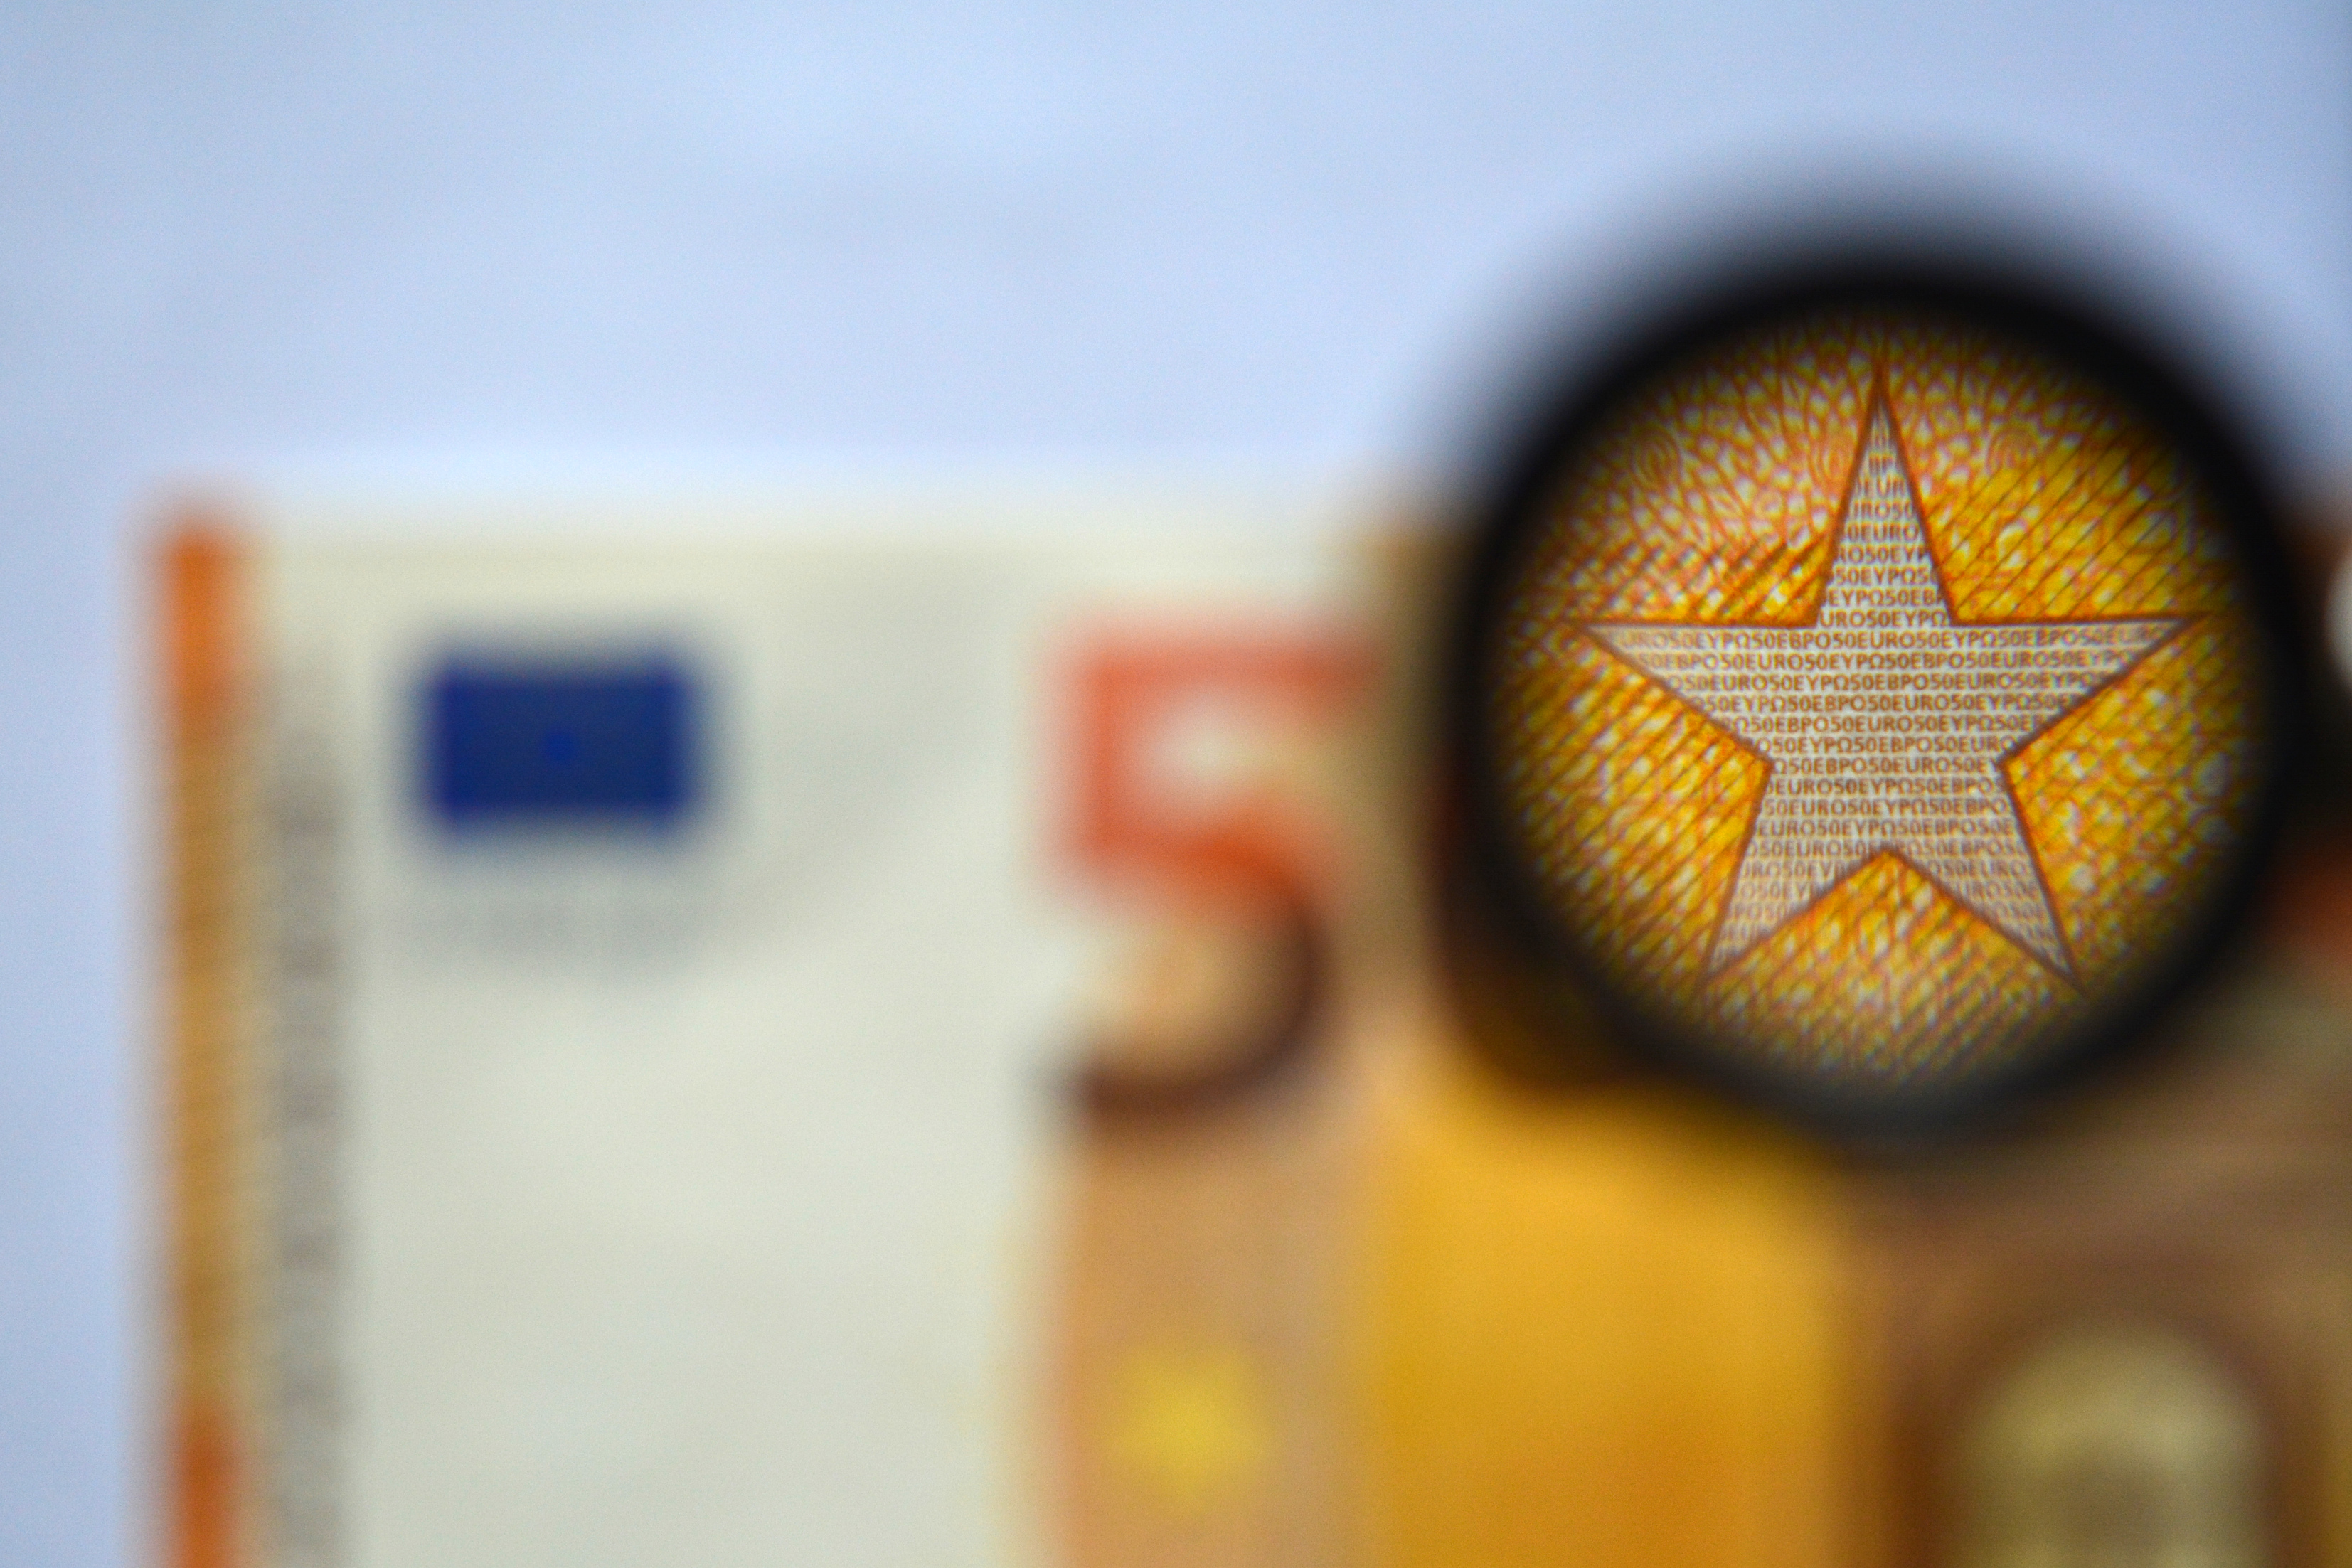
\includegraphics[width=7truecm]{slike/02_photos_lupa.jpg}\hfill
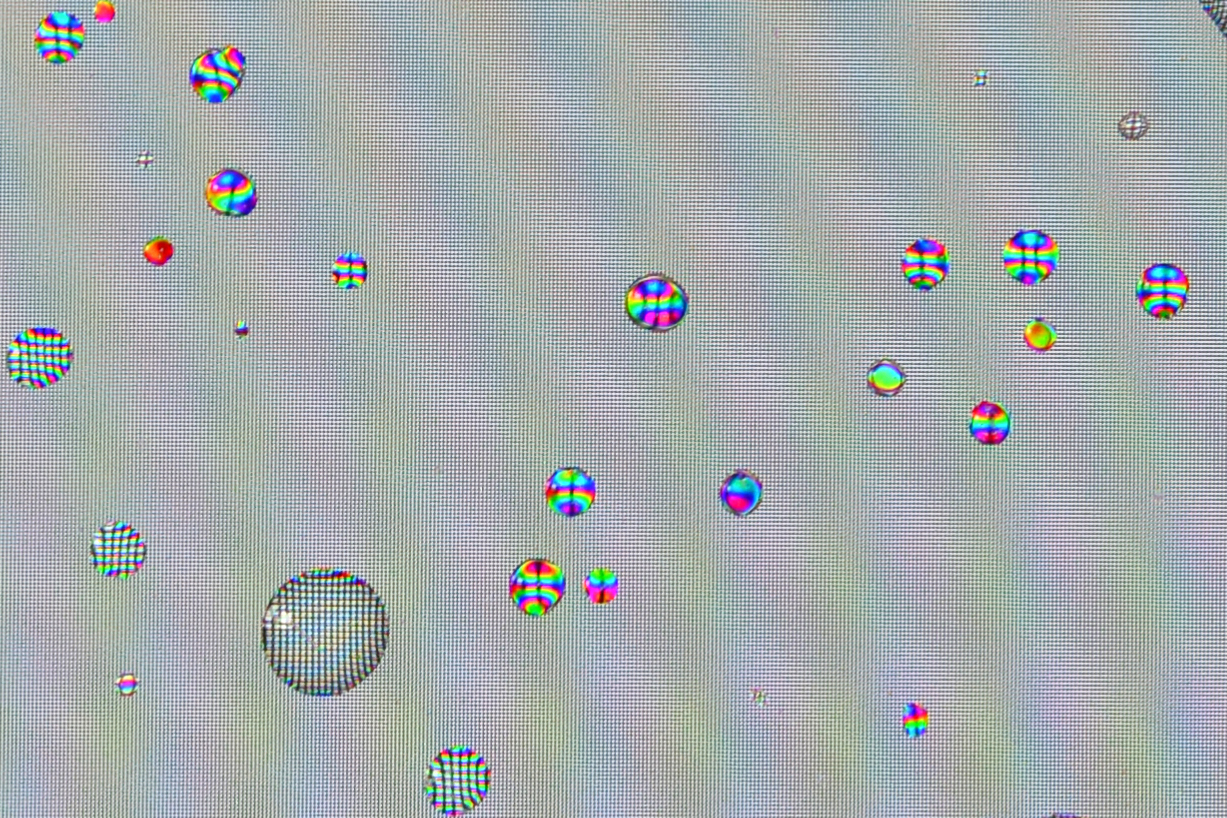
\includegraphics[width=7truecm]{slike/02_photos_kapljice.jpg}
\caption{Drobni tisk na bankovcu vidimo šele z uporabo zbiralne leče (levo). 
Drobne kapljice na zaslonu telefona delujejo kot povečevalna lupa in lahko 
razločimo posamezne rdeče, zelene in modre piksle v prikazovalniku (desno).}
\label{fig:02_photos-1}
\end{figure}

\begin{figure}[!htp]
\centering
\includegraphics[height=7truecm]{slike/02_photos_kozarec.jpg}\hfill
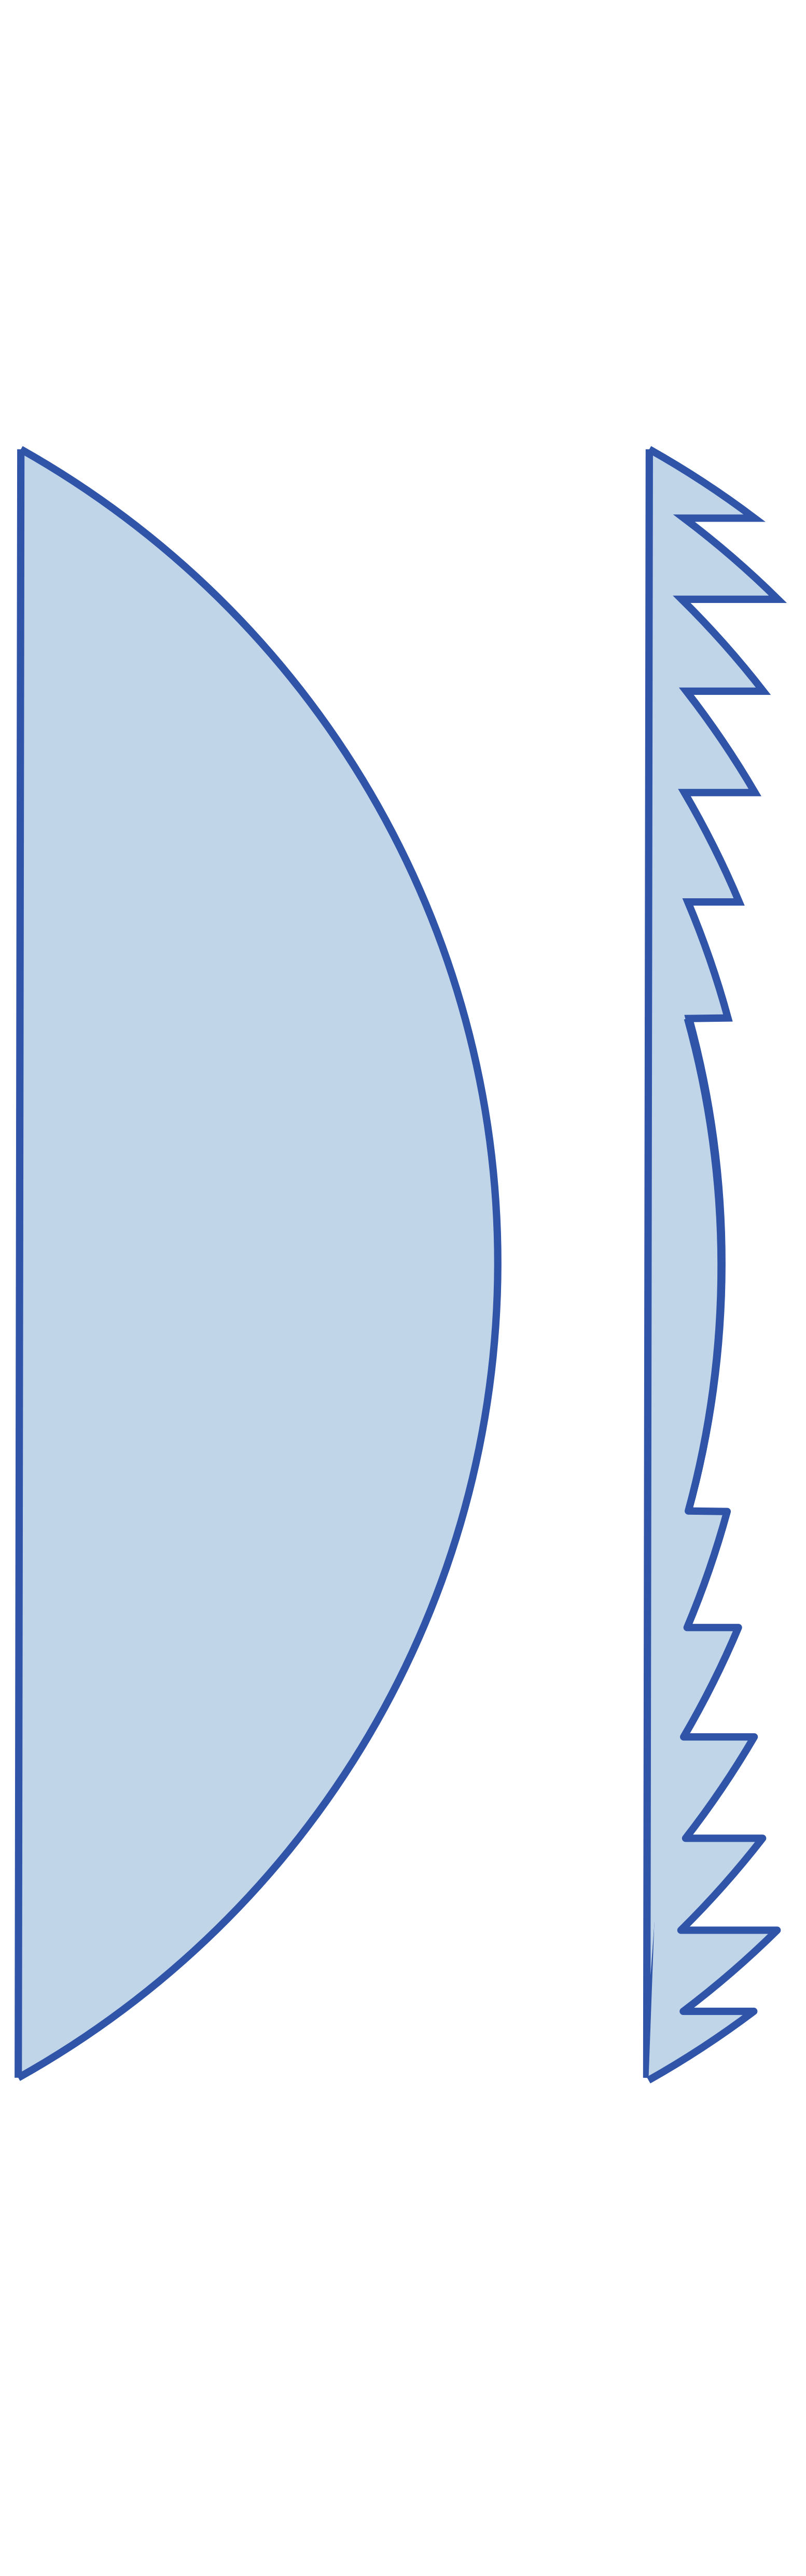
\includegraphics[height=7truecm]{slike/02_FresnelLeca.png}\hfill
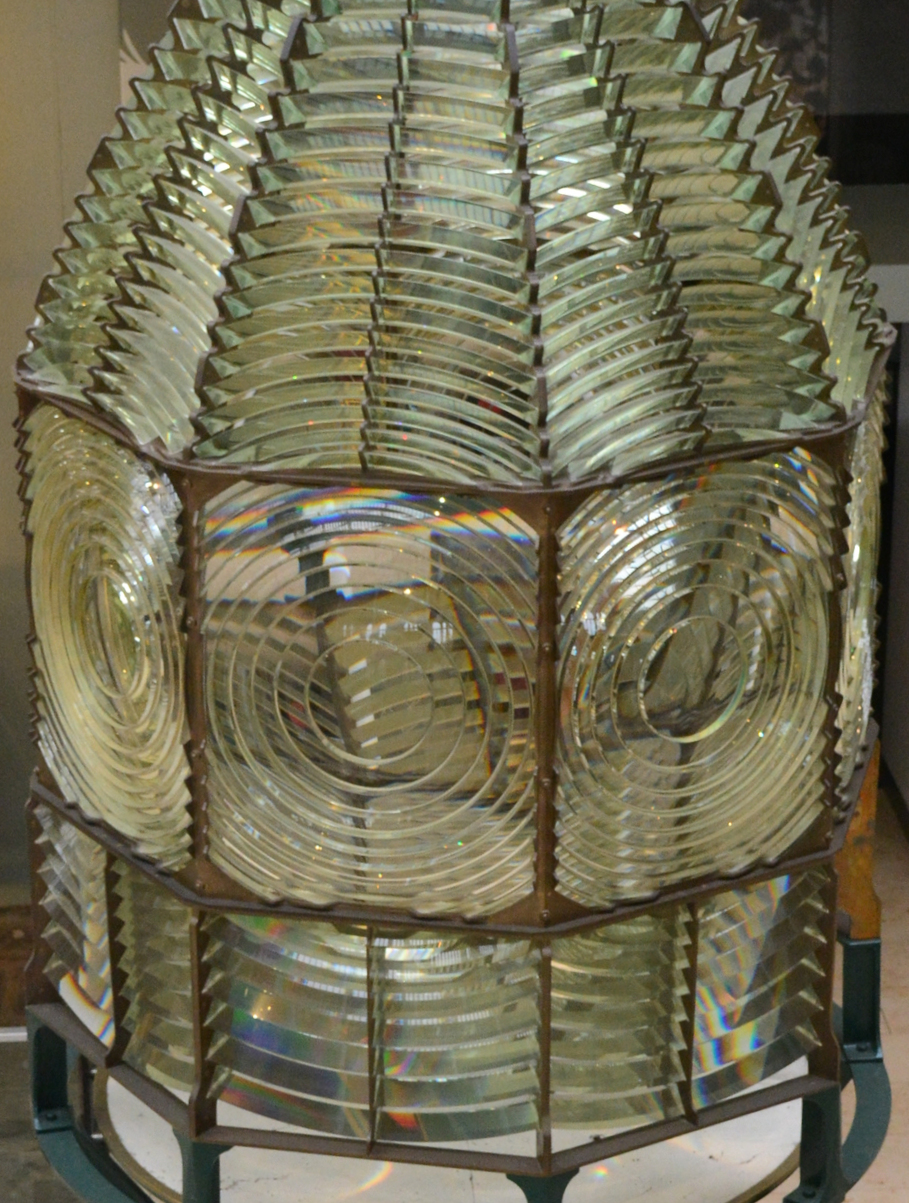
\includegraphics[height=7truecm]{slike/02_photos_svetilnik.jpg}
\caption{Kozarec, napolnjen z vodo, deluje kot zbiralna leča in 
sliko obrne (levo). Shema Fresnelove leče: na posameznih
kolobarjih je enaka ukrivljenost kot na navadni leči, vendar je celotna 
leča tanjša in lažja (sredina). Fresnelova leča na svetilniku ustvari široke 
snope svetlobe, ki so vidni od daleč (desno).}
\label{fig:02_photos-2}
\end{figure}
\vglue-1truecm
\begin{figure}[!htp]
\centering
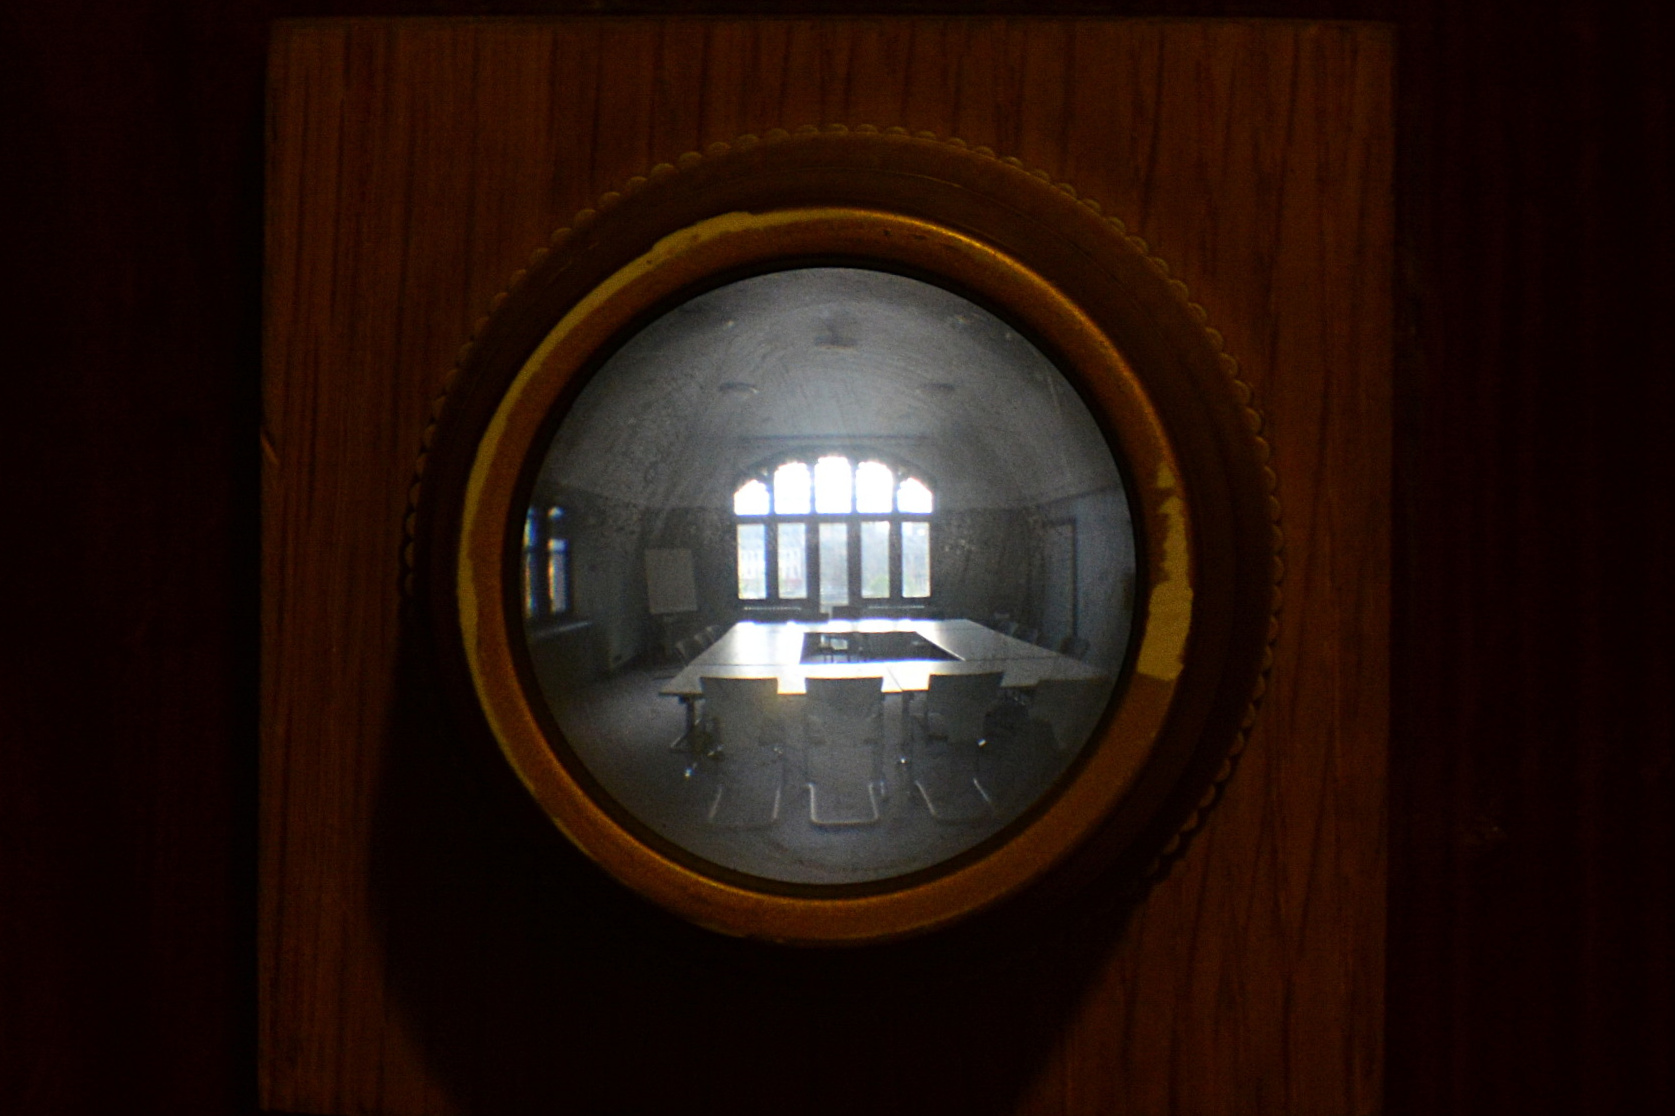
\includegraphics[width=8truecm]{slike/02_photos_peephole.jpg}
\caption{Vratno kukalo uporablja razpršilne leče, da zajamejo čim večjo sliko.}
\label{fig:02_photos-3}
\end{figure}

\newpage
Konveksna zrcala se\index{Zrcalo} uporabljajo na primer v avtomobilih kot vzvratna ali v prometu kot
cestna ogledala, da povečamo vidno polje. Podobno delujejo tudi novoletne 
okrasne bunkice ali žlica s hrbtne strani. Konkavna zrcala najdemo v
avtomobilskih žarometih, da zberejo čim več izsevane svetlobe, in za zobozdravniška
ali kozmetična zrcala, da povečajo sliko. Kot konkavno zrcalo deluje tudi 
sprednja stran žlice.

\begin{figure}[!ht]
\centering
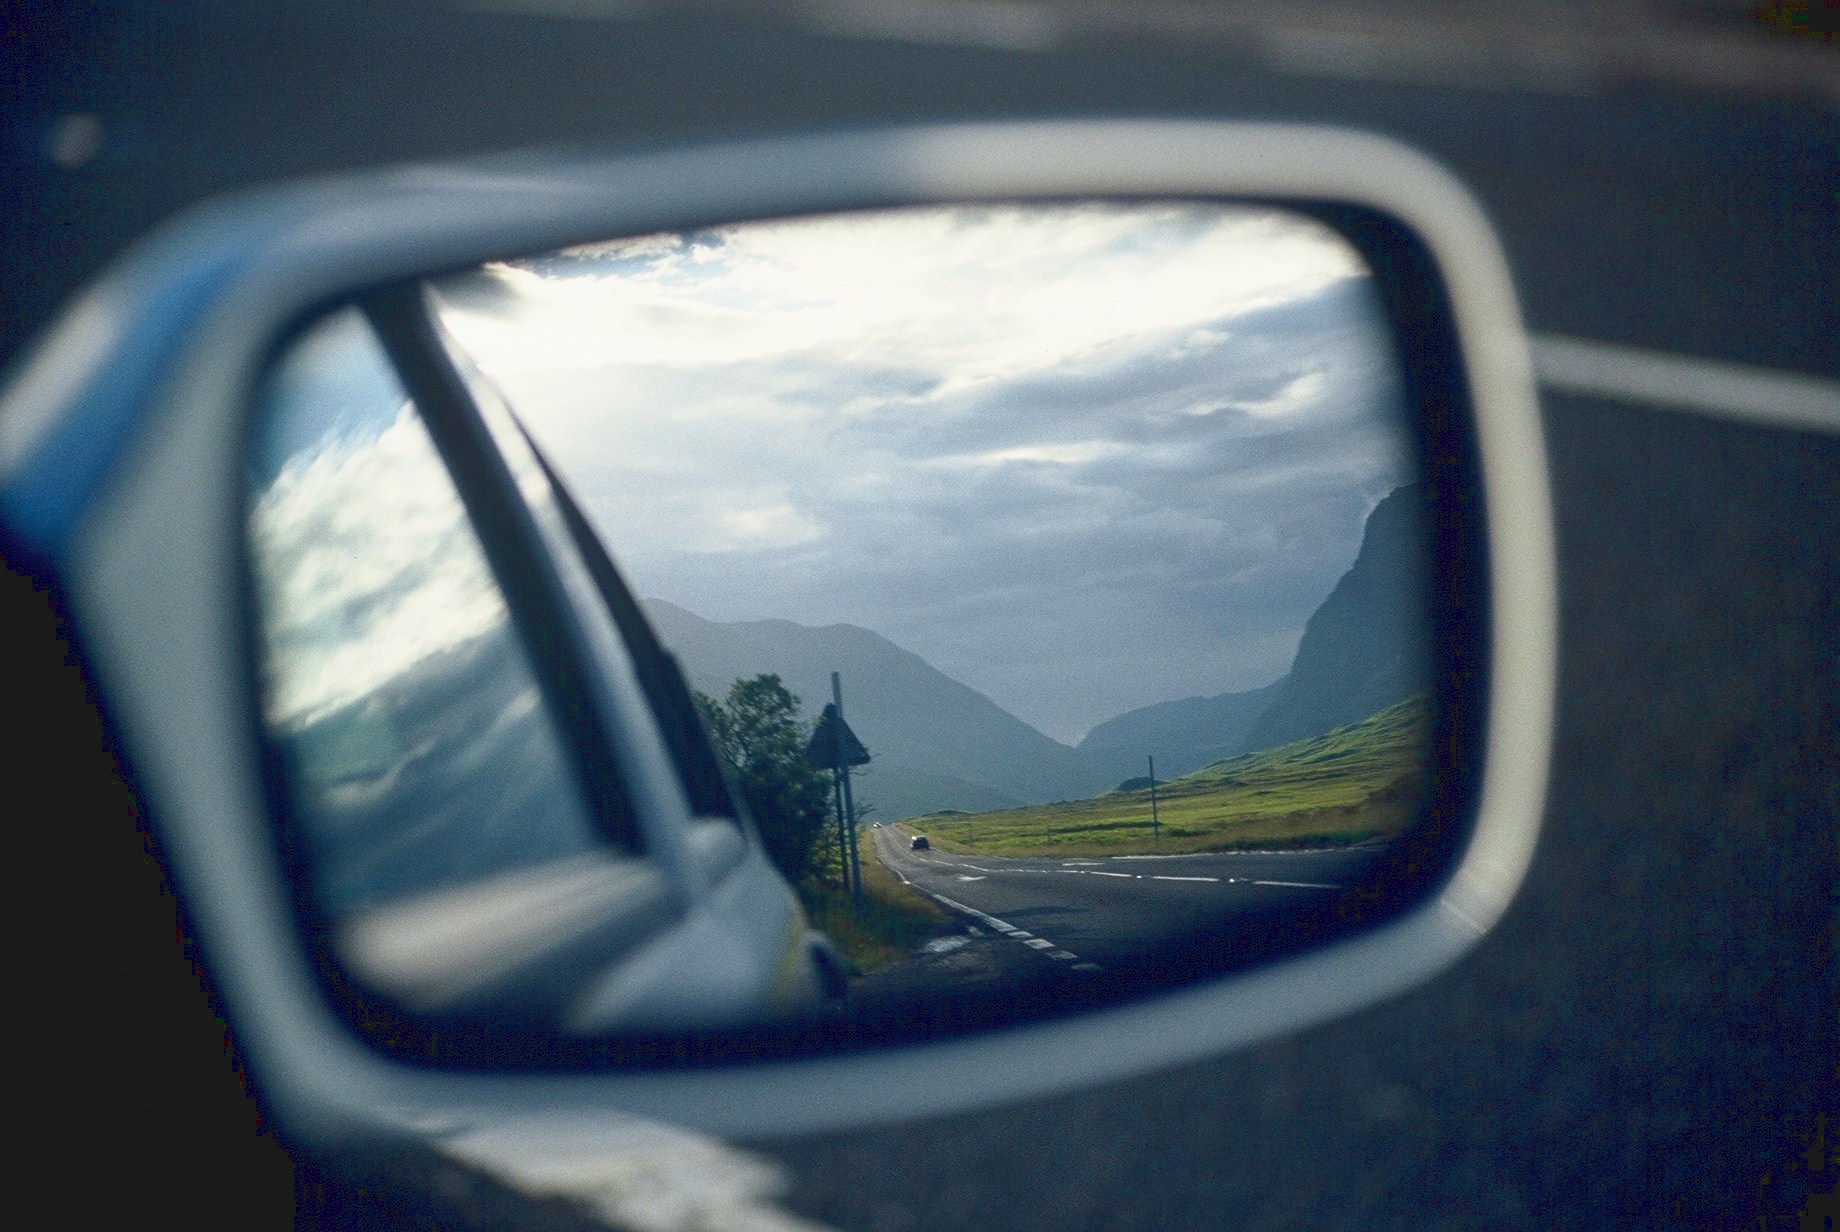
\includegraphics[width=7truecm]{slike/02_photos_avto.jpg}\hfill
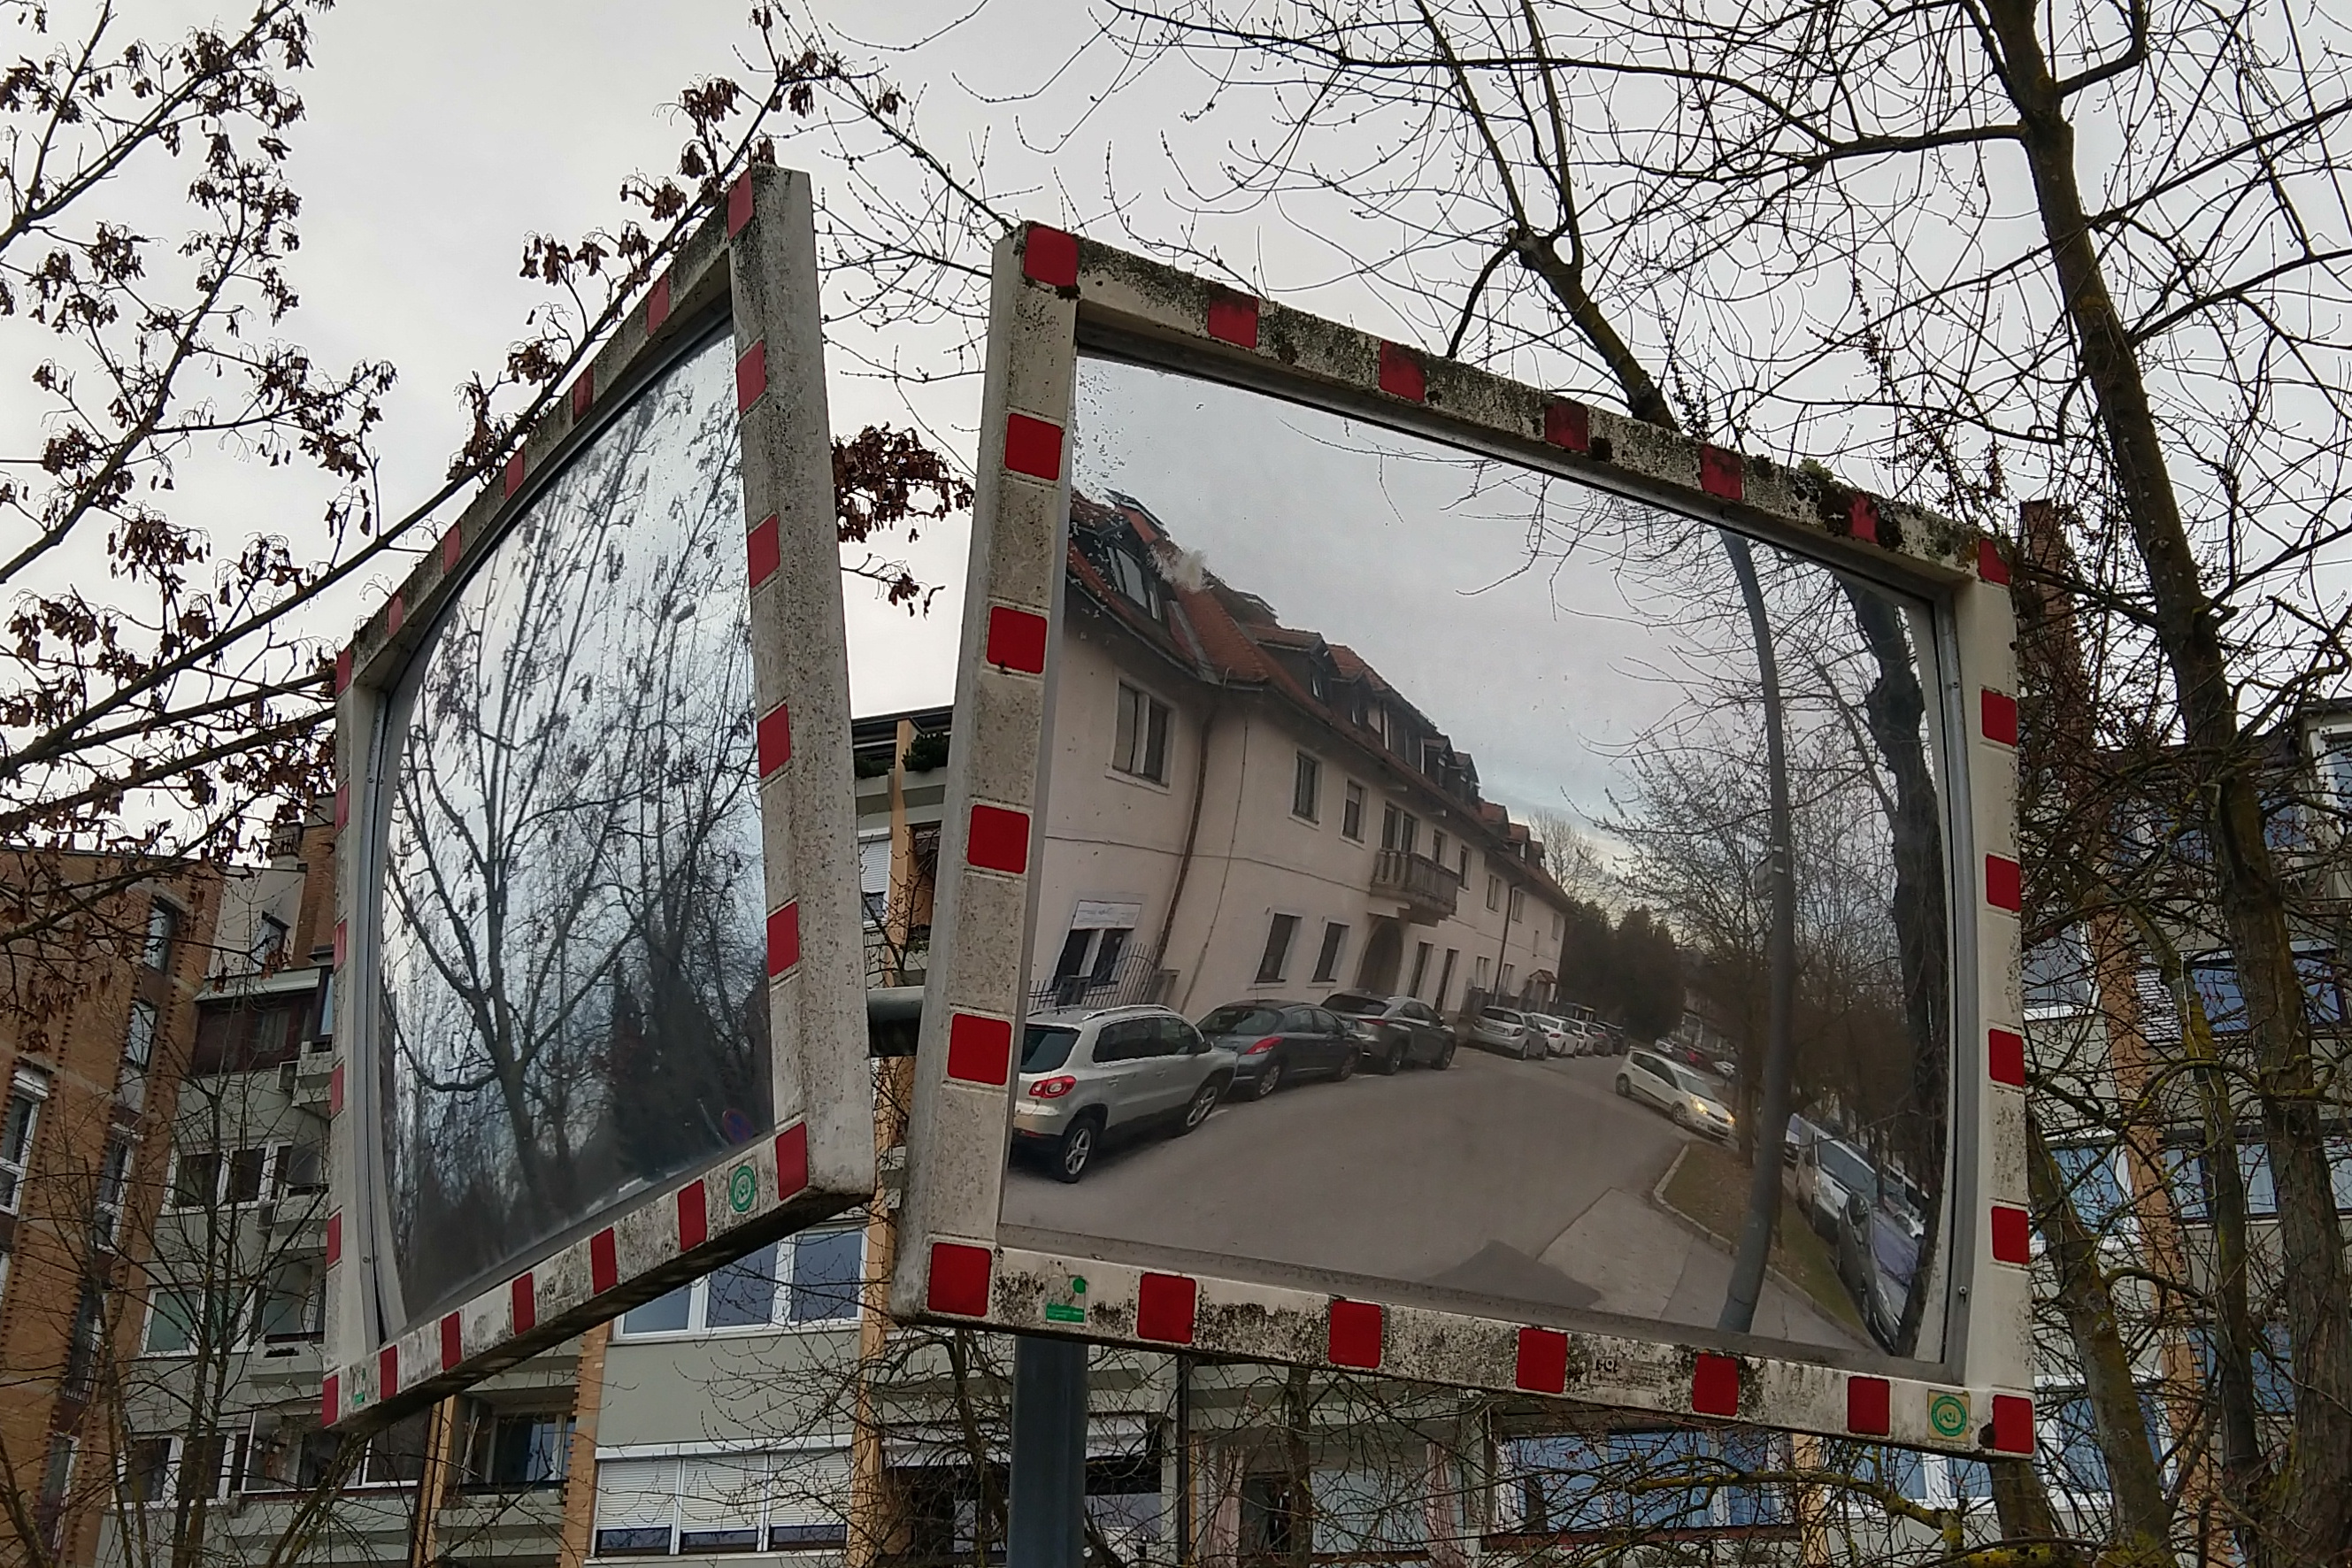
\includegraphics[width=7truecm]{slike/02_photos_cestno.jpg}
\caption{Konveksna zrcala povečajo vidno polje, zato jih uporabljamo v prometu.}
\label{fig:02_photos-4}
\end{figure}

\begin{figure}[!ht]
\centering
\includegraphics[width=7truecm]{slike/02_photos_zlica1.JPG}\hfill
\includegraphics[width=7truecm]{slike/02_photos_zlica2.JPG}
\caption{Žlica lahko deluje kot konveksno (levo) ali konkavno zrcalo (desno).}
\label{fig:02_photos-5}
\end{figure}

\chapterimage{03_Polarizacija.jpg} % Chapter heading image

\chapter{Svetloba kot elektromagnetno valovanje}
V tem poglavju bomo prešli z geometrijskega  na valovni opis svetlobe in jo 
obravnavali kot elektromagnetno valovanje. Iz Maxwellovih enačb
bomo izpeljali valovno enačbo in poiskali njene rešitve.
Zapisali bomo energijski tok
in vpeljali polarizacijo elektromagnetnega valovanja. Na koncu
bomo zapisali še valovno enačbo v prevodni snovi in vpeljali 
kompleksni lomni količnik. 

\section{Valovna enačba v neprevodni snovi}
Obravnavajmo širjenje svetlobe po homogeni, izotropni in neprevodni snovi, 
v kateri ni prostih nabojev in električnih tokov. Na splošno elektromagnetno polje
opišemo z jakostjo  $\mathbf{E}$ in gostoto električnega polja $\mathbf{D}$\index{Jakost električnega polja}
\index{Gostota električnega polja}\index{Gostota magnetnega polja}\index{Jakost magnetnega polja}
ter gostoto $\mathbf{B}$ in jakostjo magnetnega polja $\mathbf{H}$. Te vektorske
količine med seboj niso neodvisne. Za količine električnega polja velja:
\begin{equation}
\mathbf{D} = \varepsilon \varepsilon_0 \mathbf{E},
\label{eq:DE}
\end{equation}
pri čemer sta $\varepsilon$ dielektričnost (ali tudi električna permitivnost)\index{Dielektričnost}
in $\varepsilon_0$
influenčna konstanta z vrednostjo $\varepsilon_0 = 8,85 \times 10^{-12}~\si{As/Vm}$. 
Med količinami magnetnega polja velja zveza:
\begin{equation}
\mathbf{H} = \frac{\mathbf{B}}{\mu \mu_0},
\label{eq:HB}
\end{equation}
pri čemer je $\mu$ magnetna permeabilnost,\index{Permeabilnost} konstanta $\mu_0$ pa je 
indukcijska konstanta z vrednostjo $\mu_0 = 4 \pi \times 10^{-7}~\si{Vs/Am}$.
Privzeli smo, da je snov izotropna, sicer bi morali $\varepsilon$ in $\mu$ pisati v 
tenzorski obliki. Prav tako smo privzeli, da so polja v snovi dovolj šibka, da
se snov odziva linearno. Nelinearen odziv, ki ga obravnava obširno področje
nelinearne optike, presega okvir te knjige.\footnote{~Glej npr. M. Čopič in M. Vilfan, 
{\it Fotonika}, Založba FMF, 2020.}

Količine električnega in magnetnega polja med seboj povezujejo Maxwellove
enačbe:\index{Maxwellove enačbe}
\boxeq{eq:Maxwell1}{
\nabla\times\mathbf{H} & =\frac{\partial\mathbf{D}}{\partial t}+\mathbf{j}_e,\\
\nabla\times\mathbf{E} & =-\frac{\partial\mathbf{B}}{\partial t}\label{eq:Maxwell2},\\
\nabla\cdot\mathbf{D} & =\varrho_{e}\label{eq:Maxwell3}, \\
\nabla\cdot\mathbf{B} & =0.\label{eq:Maxwell4}
}

Enačbe smo zaradi splošnosti zapisali v celotni obliki. Mi bomo 
obravnavali le primer, ko sta gostota električnega toka $\mathbf{j}_e$ in 
gostota prostih nabojev $\varrho_e$ enaki nič.\index{Amp\`{e}rov zakon}
\index{Faradayev zakon}\index{Gaussov zakon}\index{Gaussov zakon za magnetno polje}

\begin{remark}
Prvo od zapisanih Maxwellovih enačb imenujemo tudi Amp\`{e}rov zakon,
drugo Faradayev indukcijski zakon,
tretjo Gaussov zakon in četrto po analogiji Gaussov zakon za magnetno polje.
\end{remark}

Izhajamo iz enačbe~(\ref{eq:Maxwell2}) in na njej naredimo rotor:
\begin{equation}
\nabla \times \left(\nabla\times\mathbf{E}\right) =
\nabla \times \left(-\frac{\partial \mathbf{B}}{\partial t} \right)\!\!.
\label{eq:03_01}
\end{equation}
Levo stran enačbe preoblikujemo z upoštevanjem splošne zveze:
\begin{equation}
\nabla \times (\nabla \times \mathbf{E}) = \nabla (\nabla \cdot \mathbf{E}) - \nabla^2 \mathbf{E}.
\label{eq:03_02}
\end{equation}
Jakost električnega polja $\mathbf{E}$  v prvem členu na desni najprej  
izrazimo z $\mathbf{D}$ (enačba~\ref{eq:DE}), nato pa upoštevamo še Gaussov zakon 
(enačba~\ref{eq:Maxwell3}) ob odsotnosti prostih nabojev. Sledi:
\begin{equation}
\nabla (\nabla \cdot \mathbf{E}) - \nabla^2 \mathbf{E} = \nabla \left(\nabla \cdot 
\frac{\mathbf{D}}{\varepsilon \varepsilon_0}\right) - \nabla^2 \mathbf{E} = - \nabla^2 \mathbf{E}.
\label{eq:03_03}
\end{equation}
Na desni strani enačbe~(\ref{eq:03_01}) odvoda po kraju in času zamenjamo, 
saj sta neodvisna. Upoštevamo enačbo~(\ref{eq:HB}), Amp\`{e}rov zakon (enačba~\ref{eq:Maxwell1}) 
in zvezo (\ref{eq:DE}). Dobimo:
\begin{equation}
\nabla \times \left(-\frac{\partial \mathbf{B}}{\partial t} \right) = 
- \frac{\partial}{\partial t}\left(\mu \mu_0 \nabla
\times \mathbf{H}\right) = - \mu \mu_0 \frac{\partial}{\partial t}\frac{\partial \mathbf{D}}{\partial t}
 = -\varepsilon \varepsilon_0 \mu \mu_0 \frac{\partial^2 \mathbf{E}}{\partial t^2}.
\label{eq:03_04}
\end{equation}
Z izenačenjem enačb~(\ref{eq:03_03}) in (\ref{eq:03_04}) dobimo valovno enačbo:\index{Valovna enačba}
\boxeq{eq:valovnaE}{
\nabla^2\mathbf{E} - \varepsilon \varepsilon_0 \mu \mu_0 \frac{\partial^2 \mathbf{E}}{\partial t^2} = 0.
}
Ponovimo še zapis leve strani valovne enačbe s komponentami:
\begin{equation}
\nabla^2 \mathbf{E} =  
\left[\begin{array}{c}
        \frac{\partial^2E_x}{\partial x^2} + \frac{\partial^2E_x}{\partial y^2} + \frac{\partial^2E_x}{\partial z^2}\\
        \frac{\partial^2E_y}{\partial x^2} + \frac{\partial^2E_y}{\partial y^2} + \frac{\partial^2E_y}{\partial z^2} \\
        \frac{\partial^2E_z}{\partial x^2} + \frac{\partial^2E_z}{\partial y^2} + \frac{\partial^2E_z}{\partial z^2}
      \end{array}\right]\!\!.
\label{eq:03_05}
\end{equation}
Podobno izpeljemo tudi valovno enačbo za gostoto magnetnega polja:
\begin{equation}
\nabla^2\mathbf{B} - \varepsilon \varepsilon_0 \mu \mu_0 \frac{\partial^2 \mathbf{B}}{\partial t^2} = 0.
\label{eq:valovnaB}
\end{equation}
Naša naloga bo poiskati rešitvi valovnih enačb $\mathbf{E}(\mathbf{r},t)$
in $\mathbf{B}(\mathbf{r},t)$ kot funkciji kraja $\mathbf{r}$ in časa $t$ pri danih robnih pogojih.

\section{Ravno valovanje}\index{Ravno valovanje}\index{Sinusno valovanje|see{Ravno valovanje}}
Najpreprostejša rešitev valovne enačbe je sinusno potujoče valovanje, ki ga zapišemo
v obliki:
\boxeq{eq:ravnival}{
\mathbf{E}(\mathbf{r},t) = \mathbf{E}_0 \cos \left(\mathbf{k}\cdot \mathbf{r} - \omega t + \delta\right) = 
\Re\left(\mathbf{E}_0 e^{i\mathbf{k}\cdot \mathbf{r} - i\omega t + i\delta}\right)
}
in 
\begin{equation}
\mathbf{B}(\mathbf{r},t) = \mathbf{B}_0 \cos \left(\mathbf{k}\cdot \mathbf{r} - \omega t + \delta\right) = 
\Re\left(\mathbf{B}_0 e^{i\mathbf{k}\cdot \mathbf{r} - i\omega t + i\delta}\right)\!\!.
\label{eq:ravnivalB}
\end{equation}
Pri tem nastavku sta amplitudi valovanja $\mathbf{E}_0$ in $\mathbf{B}_0$ konstantni, 
$\mathbf{k}$ označuje valovni vektor,\index{Valovni vektor}\index{Krožna frekvenca}
$\omega$ krožno frekvenco in $\delta$ konstantno fazo\index{Faza valovanja}
valovanja.

Poglejmo naprej krajevno in časovno odvisnost zapisane rešitve. Če se zaradi nazornosti 
omejimo na valovanje, ki potuje v smeri $z$, sinusno valovanje, ki ga opisuje 
enačba~(\ref{eq:ravnival}) preprosto narišemo. Ob danem trenutku (pri izbranem $t$) je odvisnost 
velikosti jakosti električnega polja od koordinate sinusna in prikazana na sliki~\ref{fig:03_sinus}.  

Vpeljemo valovno dolžino valovanja $\lambda$ kot krajevno periodo sinusnega vala.\index{Valovna dolžina}
Zanjo velja zveza $k\lambda = 2\pi$, od koder izračunamo velikost valovnega vektorja oziroma 
valovno število $k$:\index{Valovno število}
\boxeq{eq:valovnivektor}{
k = \frac{2\pi}{\lambda}.
}
Podobno narišemo sinusno odvisnost od časa na danem mestu (pri izbranem $z$). 
Časovna perioda je $t_0$, namesto krožne frekvence $\omega$ pa pogosto uporabljamo 
frekvenco valovanja $\nu$:\index{Frekvenca valovanja} 
\boxeq{eq:freq}{
\nu = \frac{1}{t_0} = \frac{\omega}{2\pi}.
}
\begin{figure}[!h]
\centering
\def\svgwidth{90truemm} 
\input{slike/03_sinus.pdf_tex}
\caption{Spreminjanje velikosti jakosti električnega polja vzdolž smeri $z$ pri ravnem valovanju 
ob nekem trenutku.}
\label{fig:03_sinus}
\vglue-4truemm
\end{figure}

Vrnimo se k nastavku (enačba~\ref{eq:ravnival}) in fazo oziroma
argument kotne funkcije označimo s $\phi$:
\begin{equation}
\phi = \mathbf{k}\cdot \mathbf{r} - \omega t + \delta.
\label{eq:03_06}
\end{equation}
Ploskve konstantne faze dobimo pri konstantnem $\phi$. Ob danem trenutku velja:\index{Ploskev konstantne faze}\index{Valovna fronta|see{Ploskev konstantne faze}}
\begin{equation}
\mathbf{k}\cdot \mathbf{r} = \phi + \omega t - \delta = \mathrm{konst.}
\label{eq:03_08}
\end{equation}
Ta pogoj opisuje enačbo ravnine, pravokotne na vektor $\mathbf{k}$. Ploskve konstantne faze
oziroma valovne fronte so torej ravnine, ki so pravokotne na $\mathbf{k}$, žarki pa so premice, ki 
so vzporedne s $\mathbf{k}$ (slika~\ref{fig:03_ravnival}). Zapisana rešitev predstavlja ravno valovanje.
\begin{figure}[ht]
\centering
\def\svgwidth{90truemm} 
\input{slike/03_ravnival.pdf_tex}
\caption{Najpreprostejša rešitev valovne enačbe je ravno valovanje, pri katerem so ploskve konstante
faze (valovne fronte) ravnine, pravokotne na valovni vektor $\mathbf{k}$.}
\label{fig:03_ravnival}
\end{figure}
\vglue-5truemm
\begin{remark}
Jakost električnega polja je realna količina, kar je razvidno tudi iz zapisa (enačba~\ref{eq:ravnival}). 
V računih pogosto uporabljamo kompleksni zapis, to je brez omejitve na realni del. To lahko 
naredimo, dokler so jakosti polja majhne in velja linearna optika. Račun s kompleksnim zapisom
je navadno precej preglednejši in preprostejši, vendar moramo na koncu računa vedno vzeti le
realni del izračunane jakosti električnega polja. 
\end{remark}

\subsection*{Fazna hitrost}\index{Fazna hitrost}
Fazna hitrost je hitrost premikanja ploskev konstantne faze oziroma valovnih front. 
Če sledimo valovni fronti, je odvod faze $\phi$ po času konstanten in iz enačbe~(\ref{eq:03_06}) 
sledi:
\begin{equation}
\frac{d\phi}{dt}= \mathbf{k}\cdot \frac{d\mathbf{r}}{dt} - \omega = 0.
\label{eq:03_09}
\end{equation}
Zanima nas potovanje vzdolž smeri vektorja $\mathbf{k}$, 
zato lahko zapišemo $\mathbf{k}\cdot \mathbf{r} = kr$. Fazna hitrost, ki je določena 
s hitrostjo premikanja ploskev konstantne faze, je potem enaka:
\begin{equation}
v_f = \frac{dr}{dt} = \frac{\omega}{k}.
\label{eq:03_10}
\end{equation}
Poiščimo zvezo med $\omega$ in $k$ in izračunajmo fazno hitrost.

Vstavimo nastavek za ravno valovanje (enačba~\ref{eq:ravnival}) v valovno enačbo (enačba~\ref{eq:valovnaE}). 
Obravnavajmo zaenkrat samo eno komponento, na koncu bomo zapis razširili na tri komponente. 
Za komponento v smeri $x$ dobimo:
\begin{align}
\nabla^2E_x &= \frac{\partial^2E_x}{\partial x^2} + \frac{\partial^2E_x}{\partial y^2} + 
\frac{\partial^2E_x}{\partial z^2} \nonumber \\
&= \left(\frac{\partial^2}{\partial x^2} + 
\frac{\partial^2}{\partial y^2} + \frac{\partial^2}{\partial z^2}\right) \left(
E_{0x} \exp\left( ik_xx+ik_yy+ik_zz -i\omega t + i\delta\right) \right)\nonumber \\
&= \left( -k_x^2 -k_y^2-k_z^2\right) E_{0x} \exp\left( ik_xx+ik_yy+ik_zz -i\omega t + i\delta\right)\nonumber \\
&= -k^2 E_{0x} \exp\left( ik_xx+ik_yy+ik_zz -i\omega t + i\delta\right) = -k^2 E_x.
\label{eq:03_11}
\end{align}
Podoben izračun naredimo še za ostali komponenti in zapišemo Helmholtzevo enačbo:\index{Helmholtzeva enačba}
\begin{equation}
\nabla^2\mathbf{E}= -k^2 \mathbf{E}.
\label{eq:03_12}
\end{equation}
Odvajajmo nastavek (enačba~\ref{eq:ravnival}) še dvakrat po času:
\begin{equation}
\frac{\partial^2 \mathbf{E}}{\partial t^2} = - \omega^2 \mathbf{E}.
\label{eq:03_13}
\end{equation}
Iz valovne enačbe (enačba~\ref{eq:valovnaE}) tako dobimo zvezo:
\begin{equation}
-k^2 \mathbf{E} + \varepsilon\varepsilon_0\mu\mu_0 \omega^2 \mathbf{E} = 0
\quad \Longrightarrow \quad
k = \sqrt{\varepsilon\varepsilon_0\mu\mu_0}\,\omega.
\label{eq:03_15}
\end{equation}
Zdaj lahko zapišemo fazno hitrost (enačba~\ref{eq:03_10}):
\begin{equation}
v_f = \frac{\omega}{k} = \frac{1}{\sqrt{\varepsilon_0\mu_0}}\frac{1}{\varepsilon\mu}.
\label{eq:fazna}
\end{equation}
Kadar se elektromagnetno valovanje širi v praznem prostoru, sta $\varepsilon = 1$ in $\mu=1$. 
Hitrost elektromagnetnega valovanja -- in s tem tudi svetlobe --\index{Hitrost svetlobe}
v praznem prostoru označimo s $c_0$:
\boxeq{eq:c0}{
c_0 = \frac{1}{\sqrt{\varepsilon_0\mu_0}}.
}
V snovi je fazna hitrost potovanja svetlobe,\index{Hitrost svetlobe!{v dielektriku}}
ki jo navadno označujemo s $c$, manjša, in sicer:
\begin{equation}
c = v_f = \frac{c_0}{\sqrt{\varepsilon\mu}} = \frac{c_0}{n}.
\label{eq:03_16}
\end{equation}
Pri tem smo vpeljali lomni količnik snovi $n = \sqrt{\varepsilon\mu}$.\index{Lomni količnik} 
V optiki večinoma obravnavamo snovi, ki niso magnetne, zato je lomni količnik kar
enak korenu iz dielektričnosti:
\boxeq{eq:n}{
n = \sqrt{\varepsilon}.
}
\vglue-3truemm
\begin{remark}
Ne smemo pozabiti, da se dielektričnost s frekvenco elektromagnetnega 
valovanja spreminja. Pri izračunu lomnega količnika moramo zato upoštevati vrednost
dielektričnosti pri  frekvenci vidne svetlobe, kar je $\nu \sim 5 \times 10^{14}~\si{s}^{-1}$. 
\end{remark}

\begin{table}[ht]
 \centering
 \small
\begin{tabular}{|l|c||l|c|} \hline  
      Snov & $n$ & Snov & $n$ \\ \hline
      zrak & 1,00027 & glicerol & 1,47\\ \hline
      voda & 1,33 & steklo & 1,4 -- 1,9\\ \hline 
      led & 1,31 & safir & 1,77\\ \hline
      etanol & 1,36 & diamant & 2,42\\ 
\hline 
\end{tabular}
  \caption{Lomni količniki nekaterih izbranih snovi}
\label{table:n}
\end{table}

Vrnimo se k hitrosti svetlobe. Z upoštevanjem enačb~(\ref{eq:valovnivektor}) in (\ref{eq:freq})
izraz za $c$ preoblikujemo:
\begin{equation}
 c = \frac{\omega}{k} = \frac{2 \pi \nu}{2 \pi/\lambda}.
 \label{eq:03_17}
\end{equation}
Sledi:
\boxeq{eq:nulambda}{
c = \nu \lambda.
}
Produkt frekvence in valovne dolžine je torej enak fazni hitrosti svetlobe. Ker 
se v snovi hitrost svetlobe zmanjša, hkrati pa frekvenca ohranja, se 
v snovi zmanjša valovna dolžina valovanja. Če je v praznem prostoru valovna dolžina
$\lambda_0$, potem je v snovi z lomnim količnikom $n$ valovna dolžina enaka:
\begin{equation}
\lambda = \frac{\lambda_0}{n}.
\label{eq:03_18}
\end{equation}
\vglue-6truemm
\begin{remark}\index{Valovna dolžina}
Valovna dolžina vidne svetlobe v praznem prostoru sega od okoli $350~\si{nm}$, kar
vidimo kot temno vijolično barvo, do okoli $780~\si{nm}$, kar zaznamo kot temno rdečo 
barvo. Tem valovnim dolžinam ustrezajo frekvence od približno 
$4\times10^{14}~\si{s}^{-1}$ do približno $9\times10^{14}~\si{s}^{-1}$.
\end{remark}

\subsection*{Smeri vektorjev $\mathbf{E}$, $\mathbf{B}$ in $\mathbf{k}$}
Nadaljujmo z obravnavo elektromagnetnega valovanja v homogeni in izotropni snovi. 
Valovanje naj bo v obliki ravnega potujočega sinusnega valovanja, pri čemer se poslužimo praktičnega kompleksnega zapisa:
\begin{equation}
\mathbf{E}(\mathbf{r},t) = \mathbf{E}_0 e^{i\mathbf{k}\cdot \mathbf{r} - i\omega t + i\delta}
\qquad \mathrm{in} \qquad
\mathbf{B}(\mathbf{r},t) = \mathbf{B}_0 e^{i\mathbf{k}\cdot \mathbf{r} - i\omega t + i\delta}.
\label{eq:ravnivalkompleks}
\end{equation}
Izhajamo iz Gaussovega zakona (enačba~\ref{eq:Maxwell3}) in upoštevamo zvezo med 
$\mathbf{D}$ in $\mathbf{E}$ (enačba~\ref{eq:DE}): 
\begin{equation}
\nabla \cdot \mathbf{D} = \nabla \cdot \left( \varepsilon \varepsilon_0 \mathbf{E}\right) 
= \varepsilon \varepsilon_0 \left(\nabla \cdot \mathbf{E} \right)\!.
\label{eq:03_20}
\end{equation}
Iz tega sledi, da je ob odsotnosti prostih nabojev ($\varrho_{e} = 0$) divergenca 
jakosti električnega polja v izotropni snovi enaka nič.
Zapišemo jo kot:
\begin{align}
\nabla \cdot \mathbf{E} = \frac{\partial E_x}{\partial x}+ \frac{\partial E_y}{\partial y}+
\frac{\partial E_z}{\partial z} &= \left(ik_xE_{0x} + ik_yE_{0y} + ik_zE_{0z}\right)
e^{i\mathbf{k}\cdot \mathbf{r} - i\omega t + i\delta}\nonumber\\
&= i \left( \mathbf{E}_0 \cdot \mathbf{k} \right) e^{i\mathbf{k}\cdot \mathbf{r} - i\omega t + i\delta} = 
i\, \mathbf{E} \cdot \mathbf{k} = 0.
\label{eq:03_21}
\end{align}
Skalarni produkt jakosti električnega polja in valovnega vektorja je enak nič, kadar je:\index{Jakost električnega polja}
\boxeq{eq:Ekperp}{
\mathbf{E} \perp \mathbf{k}.
}
Na enak način iz enačbe~(\ref{eq:Maxwell4}) izpeljemo zvezo:\index{Gostota magnetnega polja}
\boxeq{eq:Bkperp}{
\mathbf{B}\perp \mathbf{k}.
}
Elektromagnetno valovanje je torej v izotropni snovi transverzalno, saj sta jakost
električnega in gostota magnetnega polja pravokotni na smer širjenja svetlobe.

Poiščimo še kot med $\mathbf{E}$ in $\mathbf{B}$. Ponovno izhajamo iz Maxwellove 
enačbe, tokrat iz Faradayevega zakona (enačba~\ref{eq:Maxwell2}). Magnetno polje ravnega valovanja 
odvajamo po času in dobimo zvezo:
\begin{equation}
\nabla\times\mathbf{E} = i \omega \mathbf{B}.
\label{eq:03_22}
\end{equation}
Nato izračunamo rotor jakosti električnega polja:
\begin{equation}
\nabla \times \mathbf{E} = 
\left|
\begin{array}{ccc}
\mathbf{e}_x & \mathbf{e}_y & \mathbf{e}_z\\
\frac{\partial}{\partial x} & \frac{\partial}{\partial y} & \frac{\partial}{\partial z}\\
E_{x} & E_{y} & E_{z}
\end{array}\right|
= 
\left[
\begin{array}{c}
ik_y E_z-ik_zE_y\\
ik_z E_x-ik_xE_z\\
ik_x E_y-ik_yE_x
\end{array}\right] = 
i\, \mathbf{k}\times \mathbf{E}.
\label{eq:03_23}
\end{equation}
Rezultat vstavimo v enačbo~(\ref{eq:03_22}) in dobimo:
\begin{equation}
\mathbf{k}\times \mathbf{E} = \omega \mathbf{B}.
\label{eq:EkB}
\end{equation}
Sledi ortogonalnost jakosti električnega $\mathbf{E}$ in gostote magnetnega
polja $\mathbf{B}$:
\boxeq{eq:EBort}{
\mathbf{B}\perp \mathbf{E}.
}
S tem smo pokazali, da so v elektromagnetnem valovanju v izotropni snovi\index{Valovni vektor}
vsi trije vektorji $\mathbf{E}$, $\mathbf{B}$ in $\mathbf{k}$
med seboj paroma pravokotni. Navadno velja dogovor, da svetloba potuje
vzdolž osi $z$, $\mathbf{E}$ kaže vzdolž osi $x$ in $\mathbf{B}$ vzdolž osi $y$ (slika~\ref{fig:03_orto}).
\begin{figure}[ht]
\centering
\def\svgwidth{120truemm} 
\input{slike/03_orto.pdf_tex}
\caption{Elektromagnetno valovanje v izotropni snovi je transverzalno.}
\label{fig:03_orto}
\vglue-4truemm
\end{figure}

\subsection*{Razmerje med $\mathbf{E}_0$ in $\mathbf{B}_0$}
Ko enkrat poznamo smeri vektorjev $\mathbf{E}$ in $\mathbf{B}$ v ravnem valovanju, lahko poiščemo 
še razmerja med njunima amplitudama. Izhajamo iz enačbe~(\ref{eq:EkB}), upoštevamo
ortogonalnost vektorjev in dobimo zvezo med amplitudama:
\begin{equation}
k E_0 = \omega B_0 \quad \Longrightarrow \quad E_0 = B_0 \frac{\omega}{k}.
\label{eq:03_24}
\end{equation}
Z upoštevanjem enačbe~(\ref{eq:03_17}) sledi:
\boxeq{eq:EBc}{
E_0 = B_0c = B_0 \frac{c_0}{n}.
}
Ker je hitrost svetlobe zelo velika, so magnetna polja v elektromagnetnem valovanju 
razmeroma šibka. Na primer vrednosti 
$E_0 = 100~\si{V/m}$ ustreza $B_0 = 0,3~\si{\micro \tesla}$, kar je približno 
stokrat manj kot Zemljino magnetno polje. 

Pogosto nas zanima razmerje med $E_0$ in $H_0$. To razmerje imenujemo impedanca\index{Impedanca}
snovi in jo označimo z $Z$. Enaka je:
\begin{equation}
Z = \frac{E_0}{H_0} = \frac{E_0 \mu \mu_0}{B_0} = \mu \mu_0 c = 
\frac{\mu \mu_0}{\sqrt{\varepsilon \varepsilon_0 \mu \mu_0}} = \sqrt{\frac{\mu \mu_0}{\varepsilon \varepsilon_0}}.
\label{eq:03_25}
\end{equation}
Hitro uvidimo, da je enota za impedanco $\si{\ohm}$. V vakuumu, 
kjer sta $\varepsilon = 1$ in $\mu= 1$, je impedanca $Z_0 = 377~\si{\ohm}$.

\begin{remark}
Poleg ravnega valovanja, ki predstavlja enodimenzionalno rešitev valovne enačbe, poznamo
tudi druge rešitve, na primer sferično (krogelno)
\index{Sferično valovanje|see{Krogelno valovanje}}\index{Krogelno valovanje} ali 
cilindrično valovanje\index{Cilindrično valovanje} (slika~\ref{fig:03_sfericnival}). 
Pri\index{Ploskev konstantne faze}
sferičnem valovanju so ploskve konstantne faze krogelne lupine, ki izhajajo radialno 
simetrično iz točke izvora. Amplituda valovanja ni konstantna, ampak se zmanjšuje z oddaljenostjo 
od izhodišča kot $A = E_0/r$. V primeru cilindričnega valovanja so ploskve konstantne
faze valji, ki izhajajo iz izhodiščne premice. Tudi v tem primeru amplituda valovanja ni konstantna,
ampak pojema z oddaljenostjo od izhodiščne premice: $A = E_0/\sqrt{r}$.  Če cilindrični 
primer omejimo na ravnino, ki je pravokotna na izhodiščno premico (kar zaradi 
translacijske simetrije lahko naredimo), dobimo rešitev dvodimenzionalne valovne enačbe 
v polarnih koordinatah. 
\begin{figure}[ht]
\centering
\def\svgwidth{100truemm} 
\input{slike/03_sfericnival.pdf_tex}
\caption{Valovne fronte sferičnega valovanja so krogelne lupine (a), valovne fronte
cilindričnega valovanja pa valji (b).}
\label{fig:03_sfericnival}
\end{figure}
\end{remark}

\section{Poyntingov vektor in energijski tok}
Verjetno najpomembnejša lastnost elektromagnetnega valovanja je prenos energije. V električnem
polju gostoto energije zapišemo kot:\footnote{Glej npr. R. Podgornik in A. Vilfan, {\it Elektromagnetno polje}, 
DMFA-založništvo (2012).}\index{Gostota energije}
\begin{equation}
w_E = \frac{1}{2} \left(\mathbf{E}\cdot \mathbf{D}\right) = 
\frac{1}{2} \varepsilon \varepsilon_0 \left(\mathbf{E}\cdot \mathbf{E}\right)
= \frac{1}{2}\varepsilon \varepsilon_0 |\mathbf{E}|^2
\label{eq:03_27}
\end{equation}
in v magnetnem polju kot: 
\begin{equation}
w_B = \frac{1}{2} \left(\mathbf{B}\cdot \mathbf{H}\right) = 
\frac{1}{2\mu \mu_0} \mathbf{B}\cdot \mathbf{B} = 
\frac{1}{2\mu \mu_0} |\mathbf{B}|^2.
\label{eq:03_28}
\end{equation}
Celotna gostota energije elektromagnetnega valovanja v prostoru je vsota obeh prispevkov:
\begin{equation}
w_{EMV} = w_E + w_B = \frac{1}{2}\varepsilon \varepsilon_0 |\mathbf{E}|^2 + \frac{1}{2\mu \mu_0} |\mathbf{B}|^2.
\label{eq:03_29}
\end{equation}
Vstavimo jakost električnega (enačba~\ref{eq:ravnival}) in gostoto magnetnega polja
(enačba~\ref{eq:ravnivalB}), pri čemer za fazni zamik valovanja izberemo $\delta=0$. Sledi:
\begin{equation}
w_{EMV} = \frac{1}{2}\varepsilon \varepsilon_0 E_0^2 
\cos^2 \left(\mathbf{k}\cdot \mathbf{r} - \omega t\right)
+ \frac{1}{2\mu \mu_0} B_0^2 \cos^2 \left(\mathbf{k}\cdot \mathbf{r} - \omega t\right)\!.
\label{eq:03_30}
\end{equation}
Upoštevamo zvezo med amplitudama (enačba~\ref{eq:EBc}) in dobimo:
\begin{equation}
w_{EMV} = \left(\frac{1}{2}\varepsilon \varepsilon_0 E_0^2 + 
\frac{1}{2\mu \mu_0} \frac{E_0^2}{c^2} \right) 
\cos^2 \left(\mathbf{k}\cdot \mathbf{r} - \omega t\right)\!.
\label{eq:03_31}
\end{equation}
Ob upoštevanju izraza za hitrost valovanja (enačba~\ref{eq:fazna}) vidimo,
da sta prispevka električnega in magnetnega polja h gostoti energije elektromagnetnega valovanja
po velikosti enaka, poleg tega imata enako krajevno in časovno odvisnost:
\begin{equation}
w_{EMV} = \left(\varepsilon \varepsilon_0 E_0^2  \right) 
\cos^2 \left(\mathbf{k}\cdot \mathbf{r} - \omega t\right)\!.
\label{eq:03_32}
\end{equation}
Za vidno svetlobo je krožna frekvenca zelo velika 
($\omega \sim 3 \times 10^{15}~\si{s}^{-1}$), zato praktično vedno 
zaznavamo povprečno energijo, ki je povprečena po času čez veliko 
število nihajev. Ker je po dolgem času povprečje $\langle\cos^2(x)\rangle= 1/2$, sledi:
\boxeq{eq:w}{
\langle w \rangle = \frac{1}{2}\varepsilon \varepsilon_0 E_0^2. 
}
Gostoto energijskega ali svetlobnega toka dobimo tako, da gostoto energije
pomnožimo s hitrostjo valovanja $c$. Čeprav gre za časovno povprečje gostote
toka, ga navadno označujemo samo z $j$:\index{Gostota svetlobnega 
toka}\index{Gostota energijskega toka|see{Gostota svetlobnega toka}}
\boxeq{eq:j}{
j = \langle w \rangle c = \frac{1}{2}\varepsilon \varepsilon_0 E_0^2 c.
}
V snoveh, za katere velja $\mu = 1$, je $n = \sqrt{\varepsilon}$. Potem izraz za gostoto
energijskega toka zapišemo kot:
\begin{equation}
j = \frac{1}{2}\varepsilon \varepsilon_0 E_0^2 \frac{c_0}{\sqrt{\varepsilon}} = 
\frac{1}{2}\sqrt{\varepsilon} \varepsilon_0 E_0^2 c_0 = \frac{1}{2} \varepsilon_0 E_0^2 c_0 n.
\label{eq:03_33}
\end{equation}
Na splošno gostoto energijskega toka zapišemo v vektorski obliki, saj je poleg velikosti
pomembna tudi smer širjenja svetlobe. Velikost vektorja $\mathbf{j}$ določa 
enačba~(\ref{eq:j}), za njegovo smer pa v izotropnih snoveh velja $\mathbf{j}\parallel \mathbf{k}$,
saj se energijski tok v izotropnih snoveh širi v smeri žarkov. 
Splošnejši izraz, ki velja tudi v anizotropnih snoveh, je
zapis s Poyntingovim vektorjem $\mathbf{S}$. Vpeljemo ga kot:\index{Poyntingov vektor}
\boxeq{eq:Poyntingov}{
\mathbf{S} = \mathbf{E}\times\mathbf{H}.
}
Preverimo, da je v izotropni snovi $\langle\mathbf{S}\rangle = \mathbf{j}$, kot smo ga zapisali 
v enačbi~(\ref{eq:j}). Vpeljemo najprej vektor $\mathbf{s}$, ki je enotski vektor
v smeri valovnega vektorja, in predstavlja smer potovanja energije:
\begin{equation}
\mathbf{s} = \frac{\mathbf{k}}{k}.
\label{eq:03_34}
\end{equation}
Zapišemo:
\begin{align}
\mathbf{S}&=\mathbf{E}\times \mathbf{H} = \left( \mathbf{E}_0\times \mathbf{H}_0 \right)
\cos^2 \left(\mathbf{k}\cdot \mathbf{r} - \omega t\right) \\
& =  \left( \mathbf{E}_0 \times \frac{B_0}{\mu\mu_0}\mathbf{e}_H \right) 
\cos^2 \left(\mathbf{k}\cdot \mathbf{r} - \omega t\right) = 
\left(\mathbf{e}_E \times \mathbf{e}_H \right)E_0\frac{E_0}{c\mu\mu_0} 
\cos^2 \left(\mathbf{k}\cdot \mathbf{r} - \omega t\right)\\
&= \mathbf{s}\, \varepsilon \varepsilon_0 E_0^2\,c\, \cos^2 \left(\mathbf{k}\cdot \mathbf{r} - \omega t\right)\!.
\label{eq:03_35}
\end{align}
Pri tem smo enotska vektorja v smeri električnega in magnetnega polja označili z 
$\mathbf{e}_E$ in $\mathbf{e}_H$ ter upoštevali enačbo~(\ref{eq:fazna}). 
Povprečni Poyntingov vektor je potem:
\begin{equation}
\langle\mathbf{S}\rangle =  
\mathbf{s}\, \frac{1}{2}\varepsilon \varepsilon_0 E_0^2 c
\label{eq:03_36}
\end{equation}
in je enak gostoti svetlobnega toka (enačba~\ref{eq:j}).

Celotni energijski tok, ki se pretoči skozi dano ploskev v prostoru, izračunamo kot 
integral gostote svetlobnega toka po ploskvi:\index{Energijski tok}
\boxeq{eq:P}{
P = \int \mathbf{j}\cdot d\mathbf{S}.
}

\begin{remark}
Spomnimo se, da se pri krogelnem in cilindričnem valovanju
\index{Krogelno valovanje}\index{Cilindrično valovanje}
amplitudi valovanj
z oddaljenostjo od izhodišča ne ohranjata. To je v skladu z ohranitvijo energije, saj 
se mora celotna moč, ki je izsevana v prostor, ohranjati. V primeru krogelnega
valovanja se mora ohranjati vrednost $P = j\,4 \pi r^2$, zato $j$ pojema s kvadratom
oddaljenosti in je amplituda obratno sorazmerna z oddaljenostjo. Za cilindrično
valovanje pa se ohranja vrednost $P = j\,2\pi r L$, tako da $j$ pojema obratno
sorazmerno z oddaljenostjo in amplituda obratno sorazmerno s korenom od oddaljenosti
od izhodiščne osi. 
\end{remark}

\section{Polarizacija}
Elektromagnetno valovanje je v izotropni snovi 
transverzalno, zato zanj velja $\mathbf{E} \perp \mathbf{k}$. Orientacijo 
vektorja $\mathbf{E}$ v ravnini, ki je pravokotna na smer
širjenja svetlobe, imenujemo polarizacija.\index{Polarizacija}

Če se svetloba širi v smeri $z$, leži vektor $\mathbf{E}$ v ravnini $xy$. 
Na splošno ga lahko razstavimo na dve komponenti $E_x$ in $E_y$, ki sta
vzporedni koordinatnima osema $x$ in $y$. Jakost električnega\index{Jakost električnega polja}
polja zapišemo kot:
\begin{equation}
\mathbf{E} = E_{0x} \mathbf{e}_x \cos \left(kz - \omega t\right) + 
E_{0y} \mathbf{e}_y \cos \left(kz - \omega t + \delta\right)\!.
\label{eq:03_37}
\end{equation}
Pri tem absolutni fazni zamik valovanja ni pomemben in smo ga 
pri zapisu izpustili, ključna pa je razlika v fazi med obema 
komponentama $\delta$.\index{Faza valovanja}

Če se fazni zamik med obema komponentama $\delta(t)$ s časom 
naključno spreminja na intervalu $0<\delta <2\pi$, pravimo, da je 
svetloba nepolarizirana. Smer vektorja $\mathbf{E}$ pri nepolariziranem
valovanju v časovnem\index{Nepolarizirana svetloba}
poteku na izbranem mestu (na primer pri $z=0$) naključno preskakuje med
različnimi smermi v ravnini $xy$ z enako verjetnostjo.

V primeru polarizirane svetlobe ima $\delta$ ves čas konstantno 
vrednost oziroma vrednost, ki je poznana in počasi se spreminjajoča 
funkcija časa. Mi se osredotočimo samo na primer konstantne faze. 
Glede na vrednosti $E_{0x}$, $E_{0y}$ in $\delta$ ločimo tri tipe
polarizacije: linearno, krožno (cirkularno) in eliptično polarizacijo. 
Poglejmo jih podrobneje.

\subsection*{Linearno polarizirano valovanje}\index{Polarizacija!{linearna}}
Elektromagnetno valovanje je linearno polarizirano, kadar je smer vektorja
jakosti električnega polja konstantna. To se zgodi, ko obe komponenti nihata
ali v fazi ali v protifazi in je fazna razlika med komponentama vektorja 
jakosti električnega polja enaka večkratniku števila $\pi$. 

Zapišimo fazno razliko kot $\delta = N\pi$, pri čemer je $N$ celo število. 
Glede na sodost števila $N$ lahko ločimo dva primera -- v prvem sta obe pozitivni komponenti
vektorja $\mathbf{E}$ v fazi, v drugem pa nihata z nasprotno fazo, kar je ekvivalentno
zamenjavi predznaka ene od komponent (slika~\ref{fig:03_linpol}). 

Linearno polarizacijo na danem mestu $z$ in ob danem trenutku $t$ zapišemo
kot:
\begin{equation}
\mathbf{E} (z, t) = \left( E_{0x} \mathbf{e}_x \pm E_{0y} \mathbf{e}_y \right)
\cos \left(kz - \omega t\right)\!,
\label{eq:03_38}
\end{equation}
v izhodišču pri $z=0$ pa kot:
\begin{equation}
\mathbf{E} (z=0, t) = \left( E_{0x} \mathbf{e}_x \pm E_{0y} \mathbf{e}_y \right)
\cos \left(\omega t\right)\!.
\label{eq:03_39}
\end{equation}
Velikosti komponent $E_{0x}$ in $E_{0y}$ se na splošno razlikujeta in njuno razmerje
določa kot nagiba polarizacije glede na os $x$. Če je ena od komponent enaka nič, je 
polarizacija poravnana z drugo koordinatno osjo sistema.

\begin{figure}[ht]
\centering
\def\svgwidth{140truemm} 
\input{slike/03_linpol.pdf_tex}
\caption{Pri linearno polariziranem valovanju nihata pozitivni komponenti jakosti
električnega polja v fazi (a) ali v protifazi (b). Prikaz jakosti električnega polja
pri $t=0$ (c).}
\label{fig:03_linpol}
\end{figure}

\subsection*{Krožno (cirkularno) polarizirano valovanje}\index{Polarizacija!{krožna}}
\index{Polarizacija!{cirkularna}|see{krožna}}
Drugi primer je krožno oziroma cirkularno polarizirano valovanje. V tem primeru
se vektor električne poljske jakosti vrti v ravnini, ki je pravokotna na smer 
širjenja svetlobe. 

Krožno polarizirano valovanje nastane tedaj, ko sta komponenti jakosti 
električnega polja po velikosti enaki ($E_{0x} = E_{0y} = E_0$), fazna razlika 
med njima pa je $\delta = (N+1/2) \pi$, pri čemer je $N$ celo število. 
Zaradi periodičnosti kotnih funkcij zadošča, 
če obravnavamo samo dva primera: ko je $\delta = \pi/2$ in ko je 
$\delta = - \pi/2$. 

Na splošno krožno polarizirano valovanje
na danem mestu $z$ in ob danem času $t$ zapišemo kot:\index{Jakost električnega polja}
\begin{equation}
\mathbf{E} (z, t) = E_{0} \mathbf{e}_x \cos \left(kz - \omega t\right)
\pm E_{0} \mathbf{e}_y \sin \left(kz - \omega t\right)\!.
\label{eq:03_40}
\end{equation}
Poglejmo krožno polarizirano valovanje v izhodišču pri $z=0$ za 
$\delta = \pi/2$. Komponenta v smeri $x$ je:
\begin{equation}
E_x = E_0 \cos (-\omega t) = E_0 \cos (\omega t),
\label{eq:circx}
\end{equation}
komponenta v smeri $y$ pa:
\begin{equation}
E_y = E_0 \cos (-\omega t + \pi/2) = E_0 \sin (\omega t).
\label{eq:circy}
\end{equation}
Enačbi~(\ref{eq:circx} in \ref{eq:circy}) opisujeta krožnico v ravnini $xy$, 
kar je značilnost krožno polariziranega valovanja. Vektor jakosti
električnega polja se v tem primeru v ravnini $xy$ suče v nasprotni 
smeri urinega kazalca.

Kadar je $\delta = -\pi/2$, zapišemo valovanje v izhodiščni ravnini kot:
\begin{equation}
E_x = E_0 \cos (\omega t)
\label{eq:circxy}
\end{equation}
in 
\begin{equation}
E_y = - E_0 \sin (\omega t),
\label{eq:circxy2}
\end{equation}
vektor jakosti električnega polja pa se suče v smeri urinega kazalca.

V literaturi ni povsem enotnega dogovora o poimenovanju krožne polarizacije. 
Mi bomo uporabljali definicijo, ki se najpogosteje uporablja v optiki, to
je s stališča opazovalca. Če opazovalec gleda v smeri proti izvoru valovanja 
(v našem primeru je to vzdolž smeri $-z$), smer urinega kazalca opisuje desno 
krožno polarizirano valovanje, nasprotna smer urinega kazalca pa levo 
krožno polarizirano valovanje (slika~\ref{fig:03_cirkpol}).\index{Polarizacija!{desna krožna}}
\index{Polarizacija!{leva krožna}}
Enačbi~(\ref{eq:circx}) in (\ref{eq:circy}) s pozitivnim
$\delta$ torej v skladu z našim dogovorom opisujeta levo krožno
polarizirano valovanje, enačbi~(\ref{eq:circxy}) in (\ref{eq:circxy2}) 
z negativnim $\delta$ pa desno krožno polarizirano valovanje. 

\begin{figure}[ht]
\centering
\def\svgwidth{140truemm} 
\input{slike/03_cirkpol.pdf_tex}
\vglue-5truemm
\caption{Pri krožno polariziranem valovanju vrh vektorja
jakosti električnega polja opisuje krožnico, ki se v izhodiščni ravnini
lahko vrti v smeri urinega kazalca, kar ustreza desno krožno polariziranem valovanju (a),
ali v nasprotni smeri, kar ustreza levo krožno polariziranem valovanju (b). 
Prikaz polja desno krožno polariziranega vala ob nekem trenutku (c).}
\label{fig:03_cirkpol}
\vglue-5truemm
\end{figure}

\begin{remark}
Pri dogovoru o levi/desni krožni polarizaciji moramo biti pozorni na tri stvari. 
Prvič -- krožnost definiramo s stališča opazovalca, kar pomeni, da gledamo proti izvoru,
in ne s stališča izvora, pri čemer bi gledali vzdolž širjenja svetlobe. Drugič --
ravno valovanje vpeljemo z odvisnostjo $(\mathbf{k}\cdot \mathbf{r} - \omega t + \delta)$ in 
ne $(\omega t - \mathbf{k}\cdot \mathbf{r} + \delta)$, kot lahko ponekod zasledimo v literaturi.
Tretjič -- pri desni krožni polarizaciji se jakost polja suče v desno, če opazujemo 
časovni potek vektorja na danem mestu (slika~\ref{fig:03_cirkpol}\,a), in v levo, 
če opazujemo krajevni potek vektorja ob danem času (slika~\ref{fig:03_cirkpol}\,c).
\end{remark}

\subsection*{Eliptična polarizacija}\index{Polarizacija!{eliptična}}
Pri eliptično polariziranem valovanju, ki je najsplošnejši primer polariziranega valovanja,
konica vektorja jakosti električnega polja v ravnini, pravokotni na smer širjenja svetlobe, orisuje elipso. 
Zapišemo ga kot:\index{Jakost električnega polja}
\begin{equation}
\mathbf{E} (z, t) = E_{0x} \mathbf{e}_x \cos \left(kz - \omega t\right)
+ E_{0y} \mathbf{e}_y \cos \left(kz - \omega t + \delta\right)\!.
\label{eq:elipticnapol}
\end{equation}
Kadar je fazni zamik med posameznima komponentama $\delta = \pm \pi/2$, razlikujeta
pa se velikosti komponent, se lastni osi elipse ujemata s koordinatnima
osema $x$ in $y$. Če pa je fazni zamik med komponentama poljuben, je elipsa
zasukana glede na koordinatni sistem za nek kot $\theta$ (slika~\ref{fig:03_elipspol}). 
\begin{figure}[ht]
\centering
\def\svgwidth{120truemm} 
\input{slike/03_elipspol.pdf_tex}
\caption{Pri eliptično polariziranem valovanju vrh vektorja
jakosti električnega polja opisuje elipso. Če je fazni zamik med komponentama
$\delta = \pm \pi/2$, sta osi elipse vzporedni koordinatnima osema (a), sicer
je elipsa zasukana (b). Z $a$ in $b$ označimo polosi elipse, $\theta$ pa je
naklon elipse glede na os $x$.}
\label{fig:03_elipspol}
\vglue-3truemm
\end{figure}

Vrednost 
kota $\theta$ lahko analitično izračunamo iz enačbe:
\begin{equation}
\tan (2\theta) = \frac{2E_{0x}E_{0y}\cos \delta}{E_{0x}^2 - E_{0y}^2},
\label{eq:elipsatheta}
\end{equation}
pri čemer sta $E_{0x}$ in $E_{0y}$ amplitudi posameznih komponent.
Izračunamo še
razmerje med kratko in dolgo polosjo elipse:
\begin{equation}
\frac{b}{a} = \frac{E_{0y}\sin\delta\cos \theta}{E_{0x}\cos \theta + E_{0y}\cos\delta\sin\theta}.
\label{eq:elipsaba}
\end{equation}
Hitro uvidimo, da sta linearna in krožna polarizacija zgolj posebna
primera eliptične polarizacije: v prvem primeru je elipsa sploščena v daljico, 
v drugem primeru pa razširjena v krožnico. 

Splošno eliptično polarizirano valovanje lahko vedno
zapišemo kot vsoto dveh med seboj pravokotnih
linearno polariziranih valovanj z upoštevanjem pravega faznega zamika med njima.
Podobno lahko splošno linearno polarizacijo valovanja zapišemo kot vsoto 
dveh nasprotno usmerjenih krožno polariziranih valovanj.

\subsection*{Jonesovi vektorji in matrike}\index{Jonesov vektor}
Najpriročnejši zapis polarizacije je z dvodimenzionalnimi 
vektorji, ki jih imenujemo Jonesovi vektorji.  Izhajamo iz kompleksnega zapisa
jakosti električnega polja $\mathbf{E}$ za valovanje, ki se širi v smeri osi $z$.
Komponenti $x$ in $y$ sestavimo v vektor:
\begin{equation}
\mathbf{E} = 
\left[\begin{array}{c}
E_{0x} e^{ikz - i\omega t}\\
E_{0y} e^{ikz - i\omega t + i \delta}\\
\end{array}\right]
= e^{ikz - i\omega t} 
\left[\begin{array}{c}
E_{0x}\\
E_{0y} e^{i \delta}\\
\end{array}\right]\!\!,
\label{eq:03_41}
\end{equation}
pri čemer ne upoštevamo absolutne faze valovanja. 
Pri vektorskem zapisu polarizacije krajevno-časovni del v eksponentu izpustimo, saj 
je za obe komponenti enak. Poleg tega vektor navadno normiramo in 
polarizacijo zapišemo z vektorjem:
\boxeq{eq:Jones}{
\mathbf{J} = \frac{1}{\sqrt{E_{0x}^2+E_{0y}^2}}
\left[\begin{array}{c}
E_{0x}\\
E_{0y} e^{i \delta}\\
\end{array}\right]\!\!,
}
ki ga imenujemo Jonesov vektor, po ameriškem fiziku Robertu Clarku Jonesu (1916--2004).\index{Jones, Robert Clark}

Zapišimo nekaj najznačilnejših Jonesovih vektorjev. Za svetlobo, ki 
je linearno polarizirana v smeri $x$, je Jonesov vektor oblike:\index{Polarizacija!{linearna}}
\begin{equation}
\mathbf{J} = \left[\begin{array}{c}
1\\
0\\
\end{array}\right]\!\!.
\label{eq:03_42}
\end{equation}
Podobno svetlobo, ki je linearno polarizirana v smeri $y$, zapišemo kot:
\begin{equation}
\mathbf{J} = \left[\begin{array}{c}
0\\
1\\
\end{array}\right]\!\!.
\label{eq:03_43}
\end{equation}
Če je linearna polarizacija nagnjena za nek kot, sta komponenti enaki projekciji
enotskega vektorja na osi $x$ in $y$. Za nagib $45\si{\degree}$ je
Jonesov vektor:
\begin{equation}
\mathbf{J} = \frac{1}{\sqrt{2}}\left[\begin{array}{c}
1\\
1\\
\end{array}\right]
\label{eq:03_44}
\end{equation}
in za nagib v smeri $-45\si{\degree}$:
\begin{equation}
\mathbf{J} = \frac{1}{\sqrt{2}}\left[\begin{array}{c}
1\\
-1\\
\end{array}\right]\!\!.
\label{eq:03_45}
\end{equation}
Zapišimo še Jonesov vektor za krožno polarizirano
valovanje. Za tako valovanje sta komponenti po velikosti enaki $E_0$, 
razlikujeta pa se v fazi za $\pm \pi/2$.\index{Polarizacija!{krožna}}
Po dogovoru desno krožno polarizirano valovanje zapišemo kot:\index{Polarizacija!{desna krožna}}
\begin{equation}
\mathbf{J} = \frac{1}{\sqrt{E_{0x}^2+E_{0y}^2}}
\left[\begin{array}{c}
E_{0x}\\
E_{0y} e^{i \delta}\\
\end{array}\right] = 
\frac{E_0}{\sqrt{2}E_{0}}
\left[\begin{array}{c}
1\\
e^{-i \pi/2}\\
\end{array}\right] =
\frac{1}{\sqrt{2}}
\left[\begin{array}{c}
1\\
-i\\
\end{array}\right]\!\!.
\label{eq:03_46}
\end{equation}
Za levo krožno polarizirano valovanje je Jonesov\index{Polarizacija!{leva krožna}}
vektor:
\begin{equation}
\mathbf{J} = \frac{1}{\sqrt{2}}
\left[\begin{array}{c}
1\\
i\\
\end{array}\right]\!\!.
\label{eq:03_47}
\end{equation}

Pristop z uporabo Jonesovih vektorjev postane uporaben pri prehodu
polariziranega valovanja skozi optične komponente, ki vplivajo na 
polarizacijo svetlobe oziroma jo spreminjajo. Komponente opišemo s tako
imenovanimi Jonesovimi matrikami, ki delujejo na Jonesove vektorje. 
Prednost takega pristopa je pri zapletenih sistemih, v katerih
na polarizacijo deluje več optičnih elementov zapored, saj
matrike za te optične elemente preprosto množimo.\index{Jonesova matrika}

Na splošno je izhodna polarizacija $\mathbf{J}_2$ enaka produktu
matrike $M$, ki predstavlja optični element,
in vektorja, ki opisuje vhodno polarizacijo $\mathbf{J}_1$:
\begin{equation}
\mathbf{J}_2 = \left[\begin{array}{c}
J_{2x}\\
J_{2y}\\
\end{array}\right] = 
\left[\begin{array}{cc}
M_{11}& M_{12}\\
M_{21}& M_{22}\\
\end{array}\right]\cdot
\left[\begin{array}{c}
J_{1x}\\
J_{1y}\\
\end{array}\right] = M \cdot \mathbf{J}_1.
\label{eq:03_48}
\end{equation}

Najpreprostejši
primer optičnega elementa, ki vpliva na polarizacijo valovanja,
je zagotovo linearni polarizator. Ta prepušča\index{Polarizator!linearni}
polarizacijo vzdolž prepustne smeri, komponento, ki
je nanjo pravokotna, pa povsem absorbira. Matrika za
linearni polarizator s prepustno smerjo $x$ je:
\begin{equation}
M = \left[\begin{array}{cc}
1 & 0 \\
0 & 0\\
\end{array}\right]\!\!.
\label{eq:03_481}
\end{equation}
Hiter račun pokaže, da matrika komponento $x$ poljubnega 
vpadnega valovanja ohrani, komponenta $y$ pa je vedno enaka nič. 
Podobno je Jonesova matrika za linearni polarizator s prepustnostjo
v smeri $y$:
\begin{equation}
M = \left[\begin{array}{cc}
0 & 0 \\
0 & 1\\
\end{array}\right]\!\!.
\label{eq:03_49}
\end{equation}
Če je polarizator nagnjen za kot $\pm45\si{\degree}$, je matrika
za prehod skozenj:
\begin{equation}
M = \frac{1}{2}\left[\begin{array}{cc}
1 & \pm 1 \\
\pm 1 & 1\\
\end{array}\right]\!\!.
\label{eq:03_50}
\end{equation}
Preprosto lahko preverimo, da je poljubno vpadno valovanje s komponentama
$E_x$ in $E_y$ po prehodu skozi tak polarizator polarizirano 
pod kotom $\pm45\si{\degree}$:
\begin{equation}
\mathbf{J} = \frac{1}{2}\left[\begin{array}{cc}
1 & \pm 1 \\
\pm 1 & 1\\
\end{array}\right]\cdot 
\left[\begin{array}{c}
J_{1x}\\
J_{1y}\\
\end{array}\right]\!\! = 
\frac{1}{2}\left[\begin{array}{c}
J_{1x} \pm J_{1y}\\
\pm J_{1x} + J_{1y}\\
\end{array}\right]\!\!=
\frac{J_{1x}\pm J_{1y}}{2}\left[\begin{array}{c}
1\\
\pm 1\\
\end{array}\right]\!\!.
\label{eq:03_51}
\end{equation}
Poglejmo še cirkularne polarizatorje, ki iz poljubne\index{Polarizator!cirkularni}
vpadne polarizacije naredijo krožno polarizacijo. Cirkulator, ki
prepušča desno krožno polarizacijo, zapišemo kot:
\begin{equation}
M = \frac{1}{2}\left[\begin{array}{cc}
1 & i \\
-i & 1\\
\end{array}\right]\!\!, 
\label{eq:03_52}
\end{equation}
cirkularni polarizator za levo krožno polarizirano svetlobo pa:
\begin{equation}
M = \frac{1}{2}\left[\begin{array}{cc}
1 & -i \\
i & 1\\
\end{array}\right]\!\!.
\label{eq:03_53}
\end{equation}
Tudi to hitro preverimo z računom:
\begin{equation}
\mathbf{J} = \frac{1}{2}\left[\begin{array}{cc}
1 & \pm i \\
\mp i & 1\\
\end{array}\right]\cdot 
\left[\begin{array}{c}
J_{1x}\\
J_{1y}\\
\end{array}\right]\!\! = 
\frac{1}{2}\left[\begin{array}{c}
J_{1x} \pm i J_{1y}\\
\mp i J_{1x} + J_{1y}\\
\end{array}\right]\!\!=
\frac{J_{1x}\pm i J_{1y}}{2}\left[\begin{array}{c}
1\\
\mp i\\
\end{array}\right]\!\!.
\label{eq:03_54}
\end{equation}

\begin{remark}
Linearni polarizatorji so navadno narejeni iz snovi, v
katerih je absorpcija za dve ortogonalni polarizaciji izrazito različna.
Ta pojav imenujemo linearni dikroizem. Najpogosteje se uporablja\index{Dikroizem!linearni}
tanka folija iz polivinil alkohola. Folijo med izdelavo raztegnejo v
eni smeri, da se dolge molekule polimera uredijo, nato pa na folijo
dodajo jod. Svetlobo, ki je polarizirana vzporedno z dolgimi molekulami,
premikanje jodovih elektronov vzdolž molekul zaduši. Premikanje v prečni
smeri ni mogoče, zato je svetloba, polarizirana pravokotno na dolge
molekule, prepuščena. 
\end{remark}

Omenimo še eno vrsto pomembnih optičnih elementov, ki vplivajo na optično
polarizacijo. To so retardacijske ali zakasnitvene ploščice, ki med 
komponentama polarizacije ustvarijo dodatni fazni zamik. 
Ploščice $\lambda/2$ tako med komponentama
ustvarijo fazni zamik velikosti $\pi$. Jonesova matrika za ploščico $\lambda/2$ je:\index{Ploščica $\lambda/2$}
\begin{equation}
M = e^{\pm i\pi/2}
\left[\begin{array}{cc}
1 & 0 \\
0 & -1\\
\end{array}\right]\!\!,
\label{eq:03_55}
\end{equation}
pri čemer vodilni eksponenti člen pogosto izpuščamo. 
Tak element spremeni desno cirkularno polarizirano valovanje v levo cirkularno polarizirano
in obratno, linearno polarizirano valovanje pa prezrcali čez os koordinatnega sistema.

Ploščico $\lambda/4$, ki med komponentama povzroči fazni zamik $\pi/2$, opišemo z matriko:\index{Ploščica $\lambda/4$}
\begin{equation}
M = e^{\pm i\pi/4}
\left[\begin{array}{cc}
1 & 0 \\
0 & \mp i\\
\end{array}\right]\!\!,
\label{eq:03_56}
\end{equation}
pri čemer velja zgornji predznak, če je hitra os v smeri $y$, in spodnji predznak, kadar
je hitra os v smeri $x$. Ta optični element na splošno iz vpadne linearne
polarizacije naredi eliptično. Če je vpadna polarizacija vzporedna z
lastnima osema ploščice, se linearna polarizacija ohranja, če pa je
zasukana pod kotom $45^\circ$, nastane iz linearnega krožno polarizirano valovanje. 

Zaenkrat smo zapisali matrike le za optične elemente, katerih osi so poravnane z lastnimi osmi
koordinatnega sistema. Jonesove matrike za elemente, ki so zasukani glede na 
koordinatni sistem, izračunamo tako, da prvotno matriko zasučemo za ustrezen kot $\vartheta$:
\begin{equation}
M(\vartheta) = R(\vartheta) \cdot M (0) \cdot R(\vartheta)^{T},
\label{eq:03_57}
\end{equation}
pri čemer je matrika $R$ matrika rotacije:
\begin{equation}
R = \left[\begin{array}{cc}
\cos \vartheta & -\sin\vartheta \\
\sin \vartheta & \cos \vartheta\\
\end{array}\right]\!\!.
\label{eq:03_58}
\end{equation}

Za konec zapišimo še Jonesovo matriko za odboj od ravnega zrcala pri
pravokotnem vpadu. Matrika je enaka:
\begin{equation}
M = \left[\begin{array}{cc}
1 & 0 \\
0 & -1\\
\end{array}\right]\!\!.
\label{eq:03_59}
\end{equation}
Naj obrat koordinatne osi ne zavaja. Ker se obrne smer 
širjenja svetlobe iz $z$ v $-z$, je treba obrniti tudi eno od lastnih osi, 
da ohranimo pozitivno orientacijo koordinatnega sistema. 

Matrike so zelo priročne za računanje prehoda svetlobe skozi več
zaporednih optičnih elementov, saj matrike enostavno množimo. Pri tem 
moramo paziti na vrstni red množenja: matriko za element, na katerega
svetloba vpade najprej, napišemo najbližje Jonesovemu vektorju za vpadno svetlobo, 
torej skrajno desno. Polarizacija svetlobe, ki prehaja skozi sistem, 
v katerem si elementi sledijo od 1 do $N$, je enaka:
\begin{equation}
\mathbf{J}_N = M_N \cdot M_{N-1} \dots M_2 \cdot M_1 \cdot \mathbf{J}_1.
\label{eq:03_60}
\end{equation}

\begin{example}{\bf Izdelava cirkularnega polarizatorja.}
\label{ex_circ}
Cirkularni polarizatorji so navadno narejeni iz linearnega polarizatorja, ki 
je zasukan za kot $45^\circ$, in ploščice $\lambda/4$. Izračunajmo prehodno 
matriko za tak sistem:\index{Polarizator!cirkularni}
\begin{equation}
M = 
\frac{e^{i\pi/4}}{2}
\left[\begin{array}{cc}
1 & 0 \\
0 & i\\
\end{array}\right]
\cdot
\left[\begin{array}{cc}
1 & 1 \\
1 & 1\\
\end{array}\right] = \frac{e^{i\pi/4}}{2}
\left[\begin{array}{cc}
1 & 1 \\
i & i\\
\end{array}\right]\!\!.
\end{equation}
Opisana kombinacija elementov iz poljubne vpadne svetlobe $(E_x, E_y)$ naredi
levo cirkularno polarizirano valovanje:
\begin{equation}
\left[\begin{array}{cc}
1 & 1 \\
i & i\\
\end{array}\right]\cdot 
\left[\begin{array}{c}
E_x\\
E_y\\
\end{array}\right] = (E_x+E_y)
\left[\begin{array}{c}
1\\
i\\
\end{array}\right]\!\!.
\end{equation}
Desni cirkularni polarizator naredimo tako, da vstopni linearni polarizator
zasučemo za $90^\circ$.
\end{example}

\begin{example}{\bf Optični izolator.} 
\label{ex_izolator}
Naj nepolarizirana svetloba vpada na linearni polarizator, 
nato pa skozi ploščico $\lambda/4$ na zrcalo, od katerega
se odbije in vrne po isti poti nazaj (slika~\ref{fig:03_OpticniIzolator}). Izračunajmo intenziteto
izhodne svetlobe, če je prepustna smer linearnega polarizatorja
zasukana za kot $45\si{\degree}$ glede na osi $x$ in $y$, lastne
osi ploščice $\lambda/4$ pa sovpadajo z osema $x$ in $y$.\index{Optični izolator}
\vglue-5truemm
\begin{figure}[h!]
\centering
\def\svgwidth{100truemm} 
\input{slike/03_optizo.pdf_tex}
\caption{Shema optičnega izolatorja, sestavljenega iz 
linearnega polarizatorja in ploščice $\lambda/4$.}
\label{fig:03_OpticniIzolator}
\end{figure}

Celotna matrika za prehod in odboj je produkt matrik:
\begin{equation}
 M = \frac{1}{2}\left[\begin{array}{cc}
1 & -1 \\
-1 & 1\\
\end{array}\right]\cdot 
\left[\begin{array}{cc}
1 & 0 \\
0 & i\\
\end{array}\right]\cdot 
\left[\begin{array}{cc}
1 & 0 \\
0 & -1\\
\end{array}\right]\cdot
\left[\begin{array}{cc}
1 & 0 \\
0 & i\\
\end{array}\right]
\frac{1}{2}\left[\begin{array}{cc}
1 &  1 \\
1 & 1\\
\end{array}\right]\!\!.
\label{eq:03_61}
\end{equation}
Srednja matrika predstavlja odboj od zrcala, pri katerem se os $x$ ohranja, 
os $y$ pa se obrne. Ker se po odboju svetloba širi v nasprotno
smer ($-z$), smo morali zapisati matriko za prehod linearnega polarizatorja,
zasukanega za kot $-45\si{\degree}$ glede na prvotni koordinatni sistem. 
Izračunamo produkt matrik, pri čemer zmnožimo najprej zunanja para, nato pa dobimo:
\begin{equation}
 M = \frac{1}{4}\left[\begin{array}{cc}
1 & -i \\
-1 & i\\
\end{array}\right]\cdot 
\left[\begin{array}{cc}
1 & 0 \\
0 & -1\\
\end{array}\right]
\cdot 
\left[\begin{array}{cc}
1 &  1 \\
i & i\\
\end{array}\right] = 
\left[\!\!\begin{array}{cc}
0 & 0\\
0 & 0\\
\end{array}\right]\!\!.
\label{eq:03_63}
\end{equation}
Produkt matrik je torej identično enak nič. Tak sestav imenujemo
optični izolator, saj se ne odbije nič svetlobe, ne glede na vpadno 
polarizacijo. 
\end{example}

\begin{example}{\bf Odboj polariziranega valovanja.}
Poglejmo sliko odbitega polariziranega valovanja. Linearno polarizirano
valovanje, ki vpada na zrcalo, se od njega odbije in je ponovno
prepuščeno skozi linearni polarizator. Odbito sliko vidimo. 
V prejšnjem primeru (primer~\ref{ex_izolator})
pa smo pokazali, da cirkularno polarizirano valovanje po odboju 
od zrcala ne prehaja več skozi prvotni cirkularni 
polarizator. Zrcalo iz desno krožno polariziranega valovanja naredi
levo krožno polarizirano valovanje in obratno, zato nazaj do predmeta
ne pride nič svetlobe (glej sliko~\ref{fig:03_CirkularniOdboj}). 
\begin{figure}[h!]
\centering
\includegraphics[width=7truecm]{slike/03_linodboj.JPG}\hfill
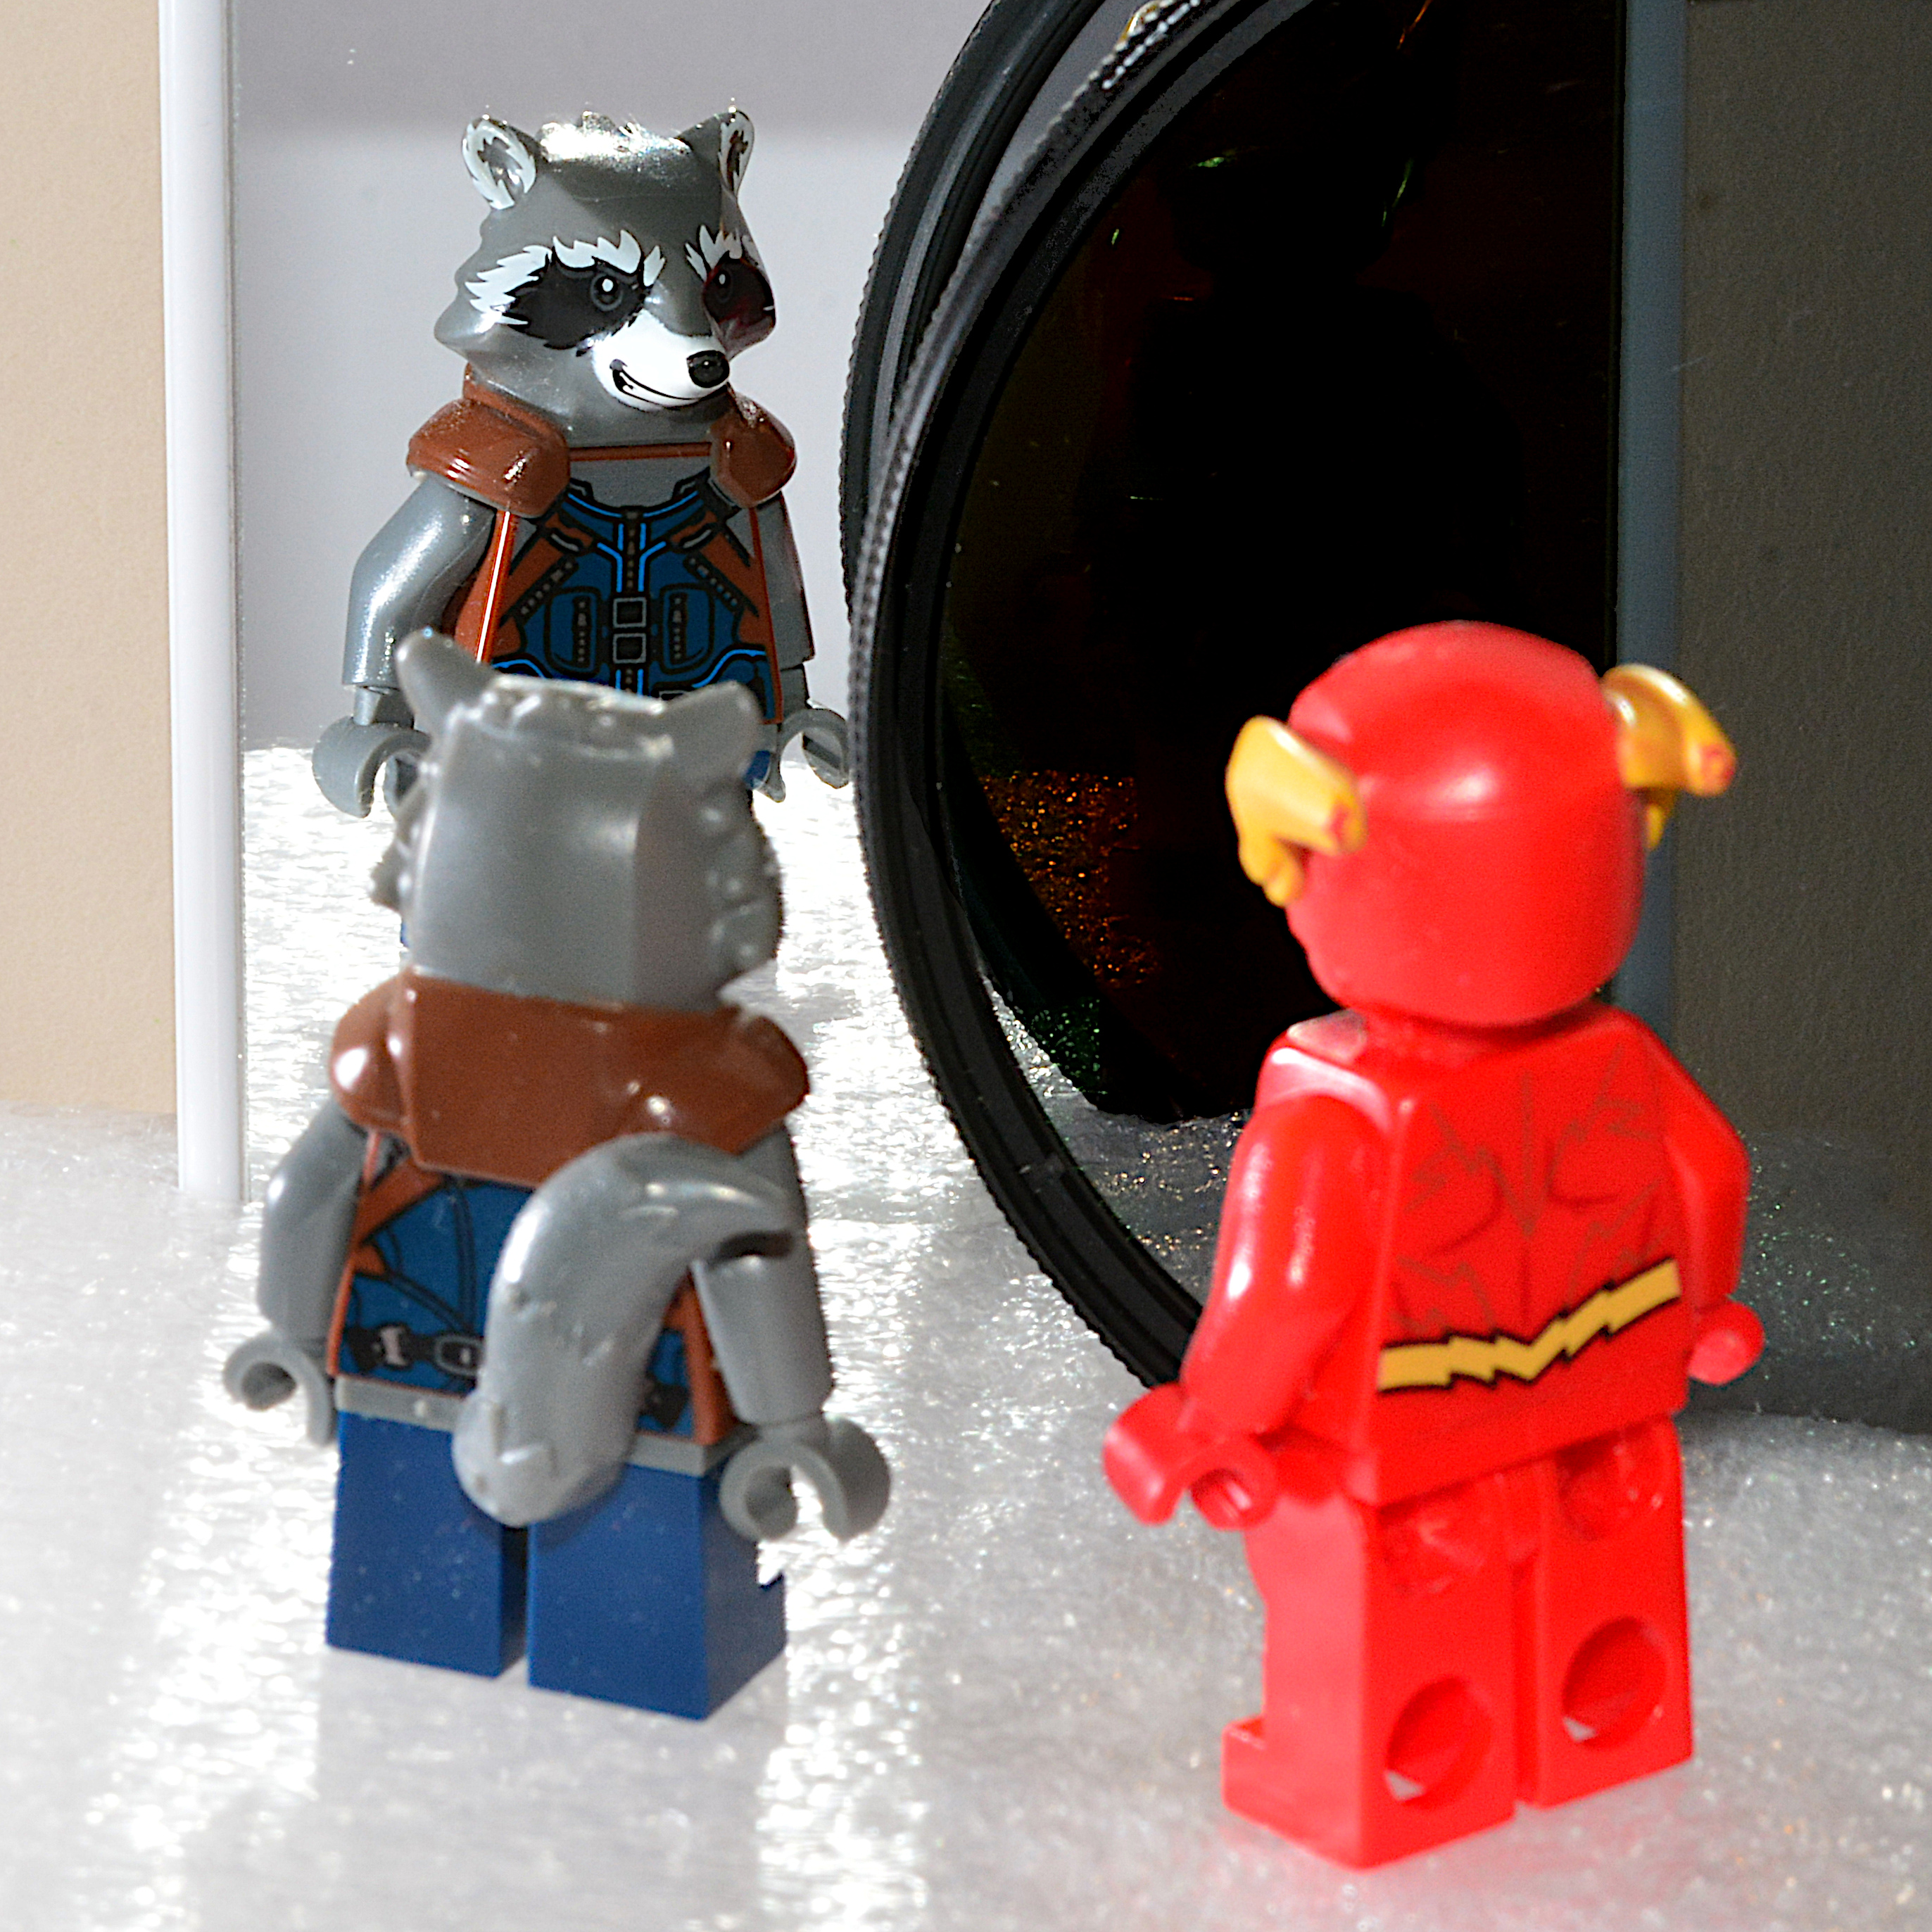
\includegraphics[width=7truecm]{slike/03_circodboj.JPG}
\caption{Linearno polarizirano valovanje pri odboju in prehodu skozi linearni polarizator
vidimo (levo). Cirkularno polarizirano valovanje se pri odboju spremeni iz 
desno polariziranega v levo polarizirano in obratno, zato pri ponovnem 
prehodu skozi cirkularni polarizator slike ni (desno).}
\label{fig:03_CirkularniOdboj}
\end{figure}
\end{example}

\begin{example}{\bf Zamenjava optičnih elementov.}
Poglejmo še učinek vrstnega reda optičnih elementov. Izberimo
kombinacijo linearnega in cirkularnega polarizatorja. V enem primeru postavimo
linearni polarizator pred cirkularnega, v drugem pa za njega. Razlika
v prepuščeni svetlobi jasno kaže pomembnost vrstnega reda optičnih
elementov in seveda tudi vrstnega reda zapisa matrik.
\begin{figure}[h!]
\centering
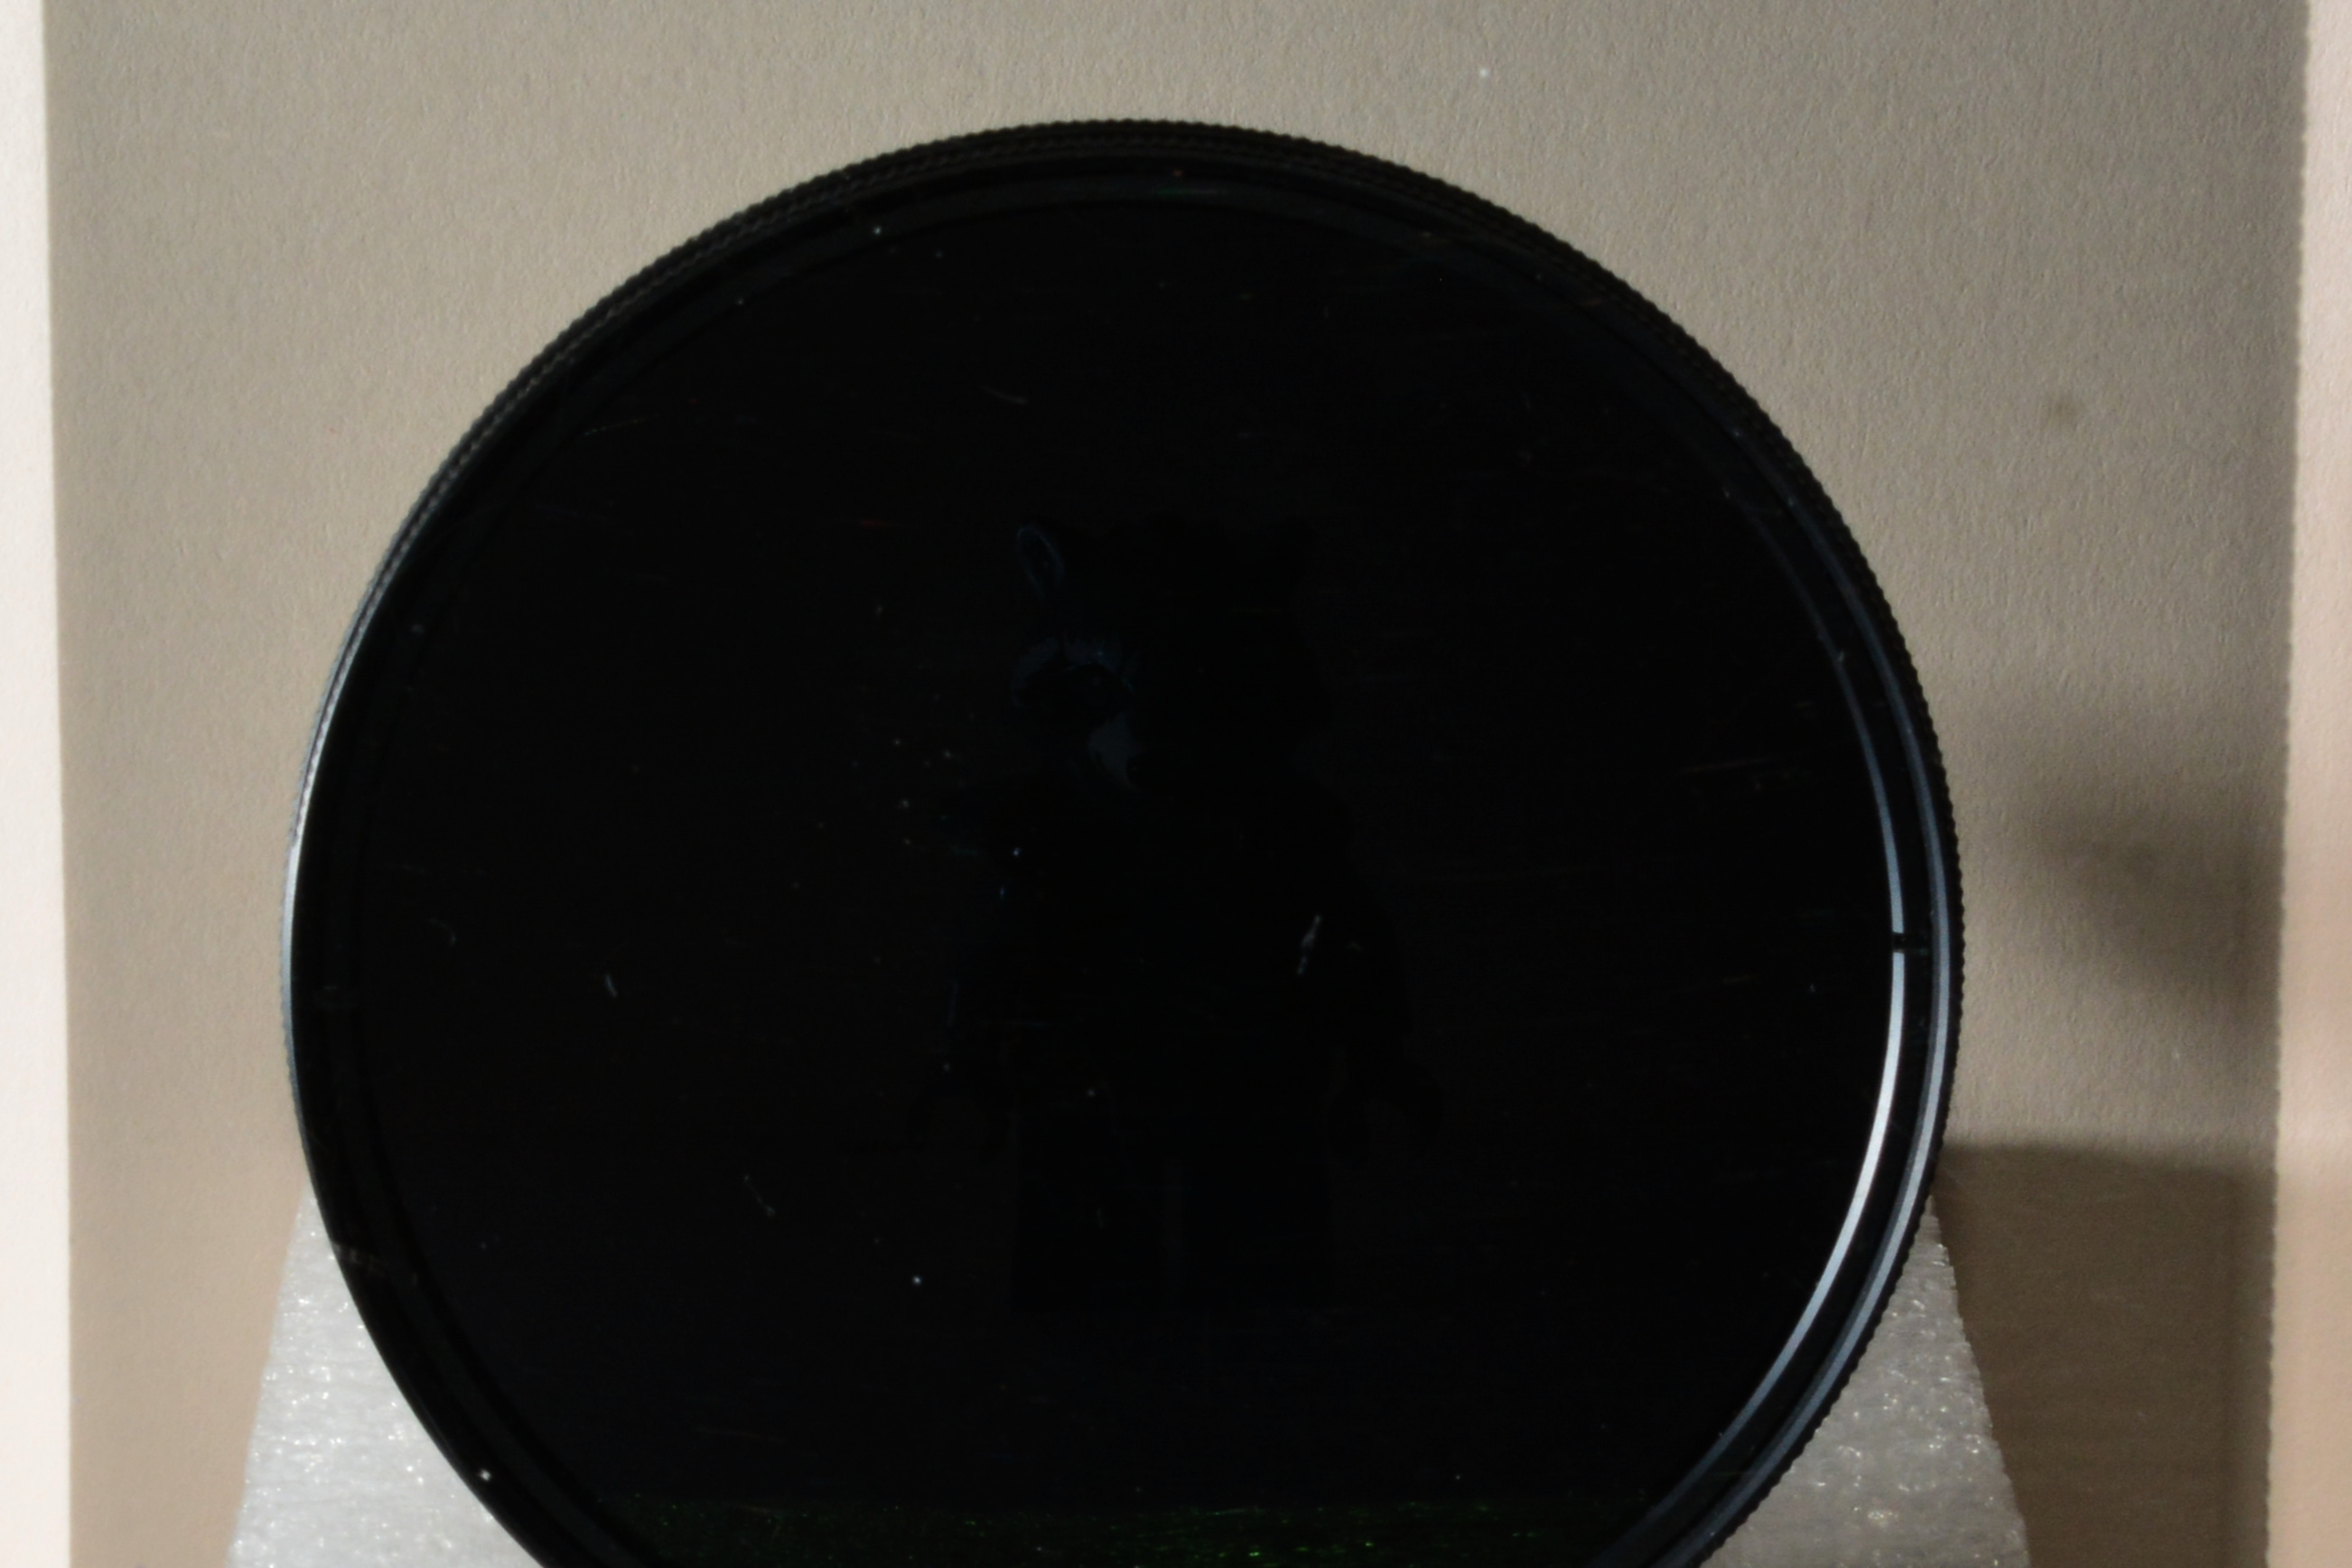
\includegraphics[width=7truecm]{slike/03_vrstnired1.JPG}\hfill
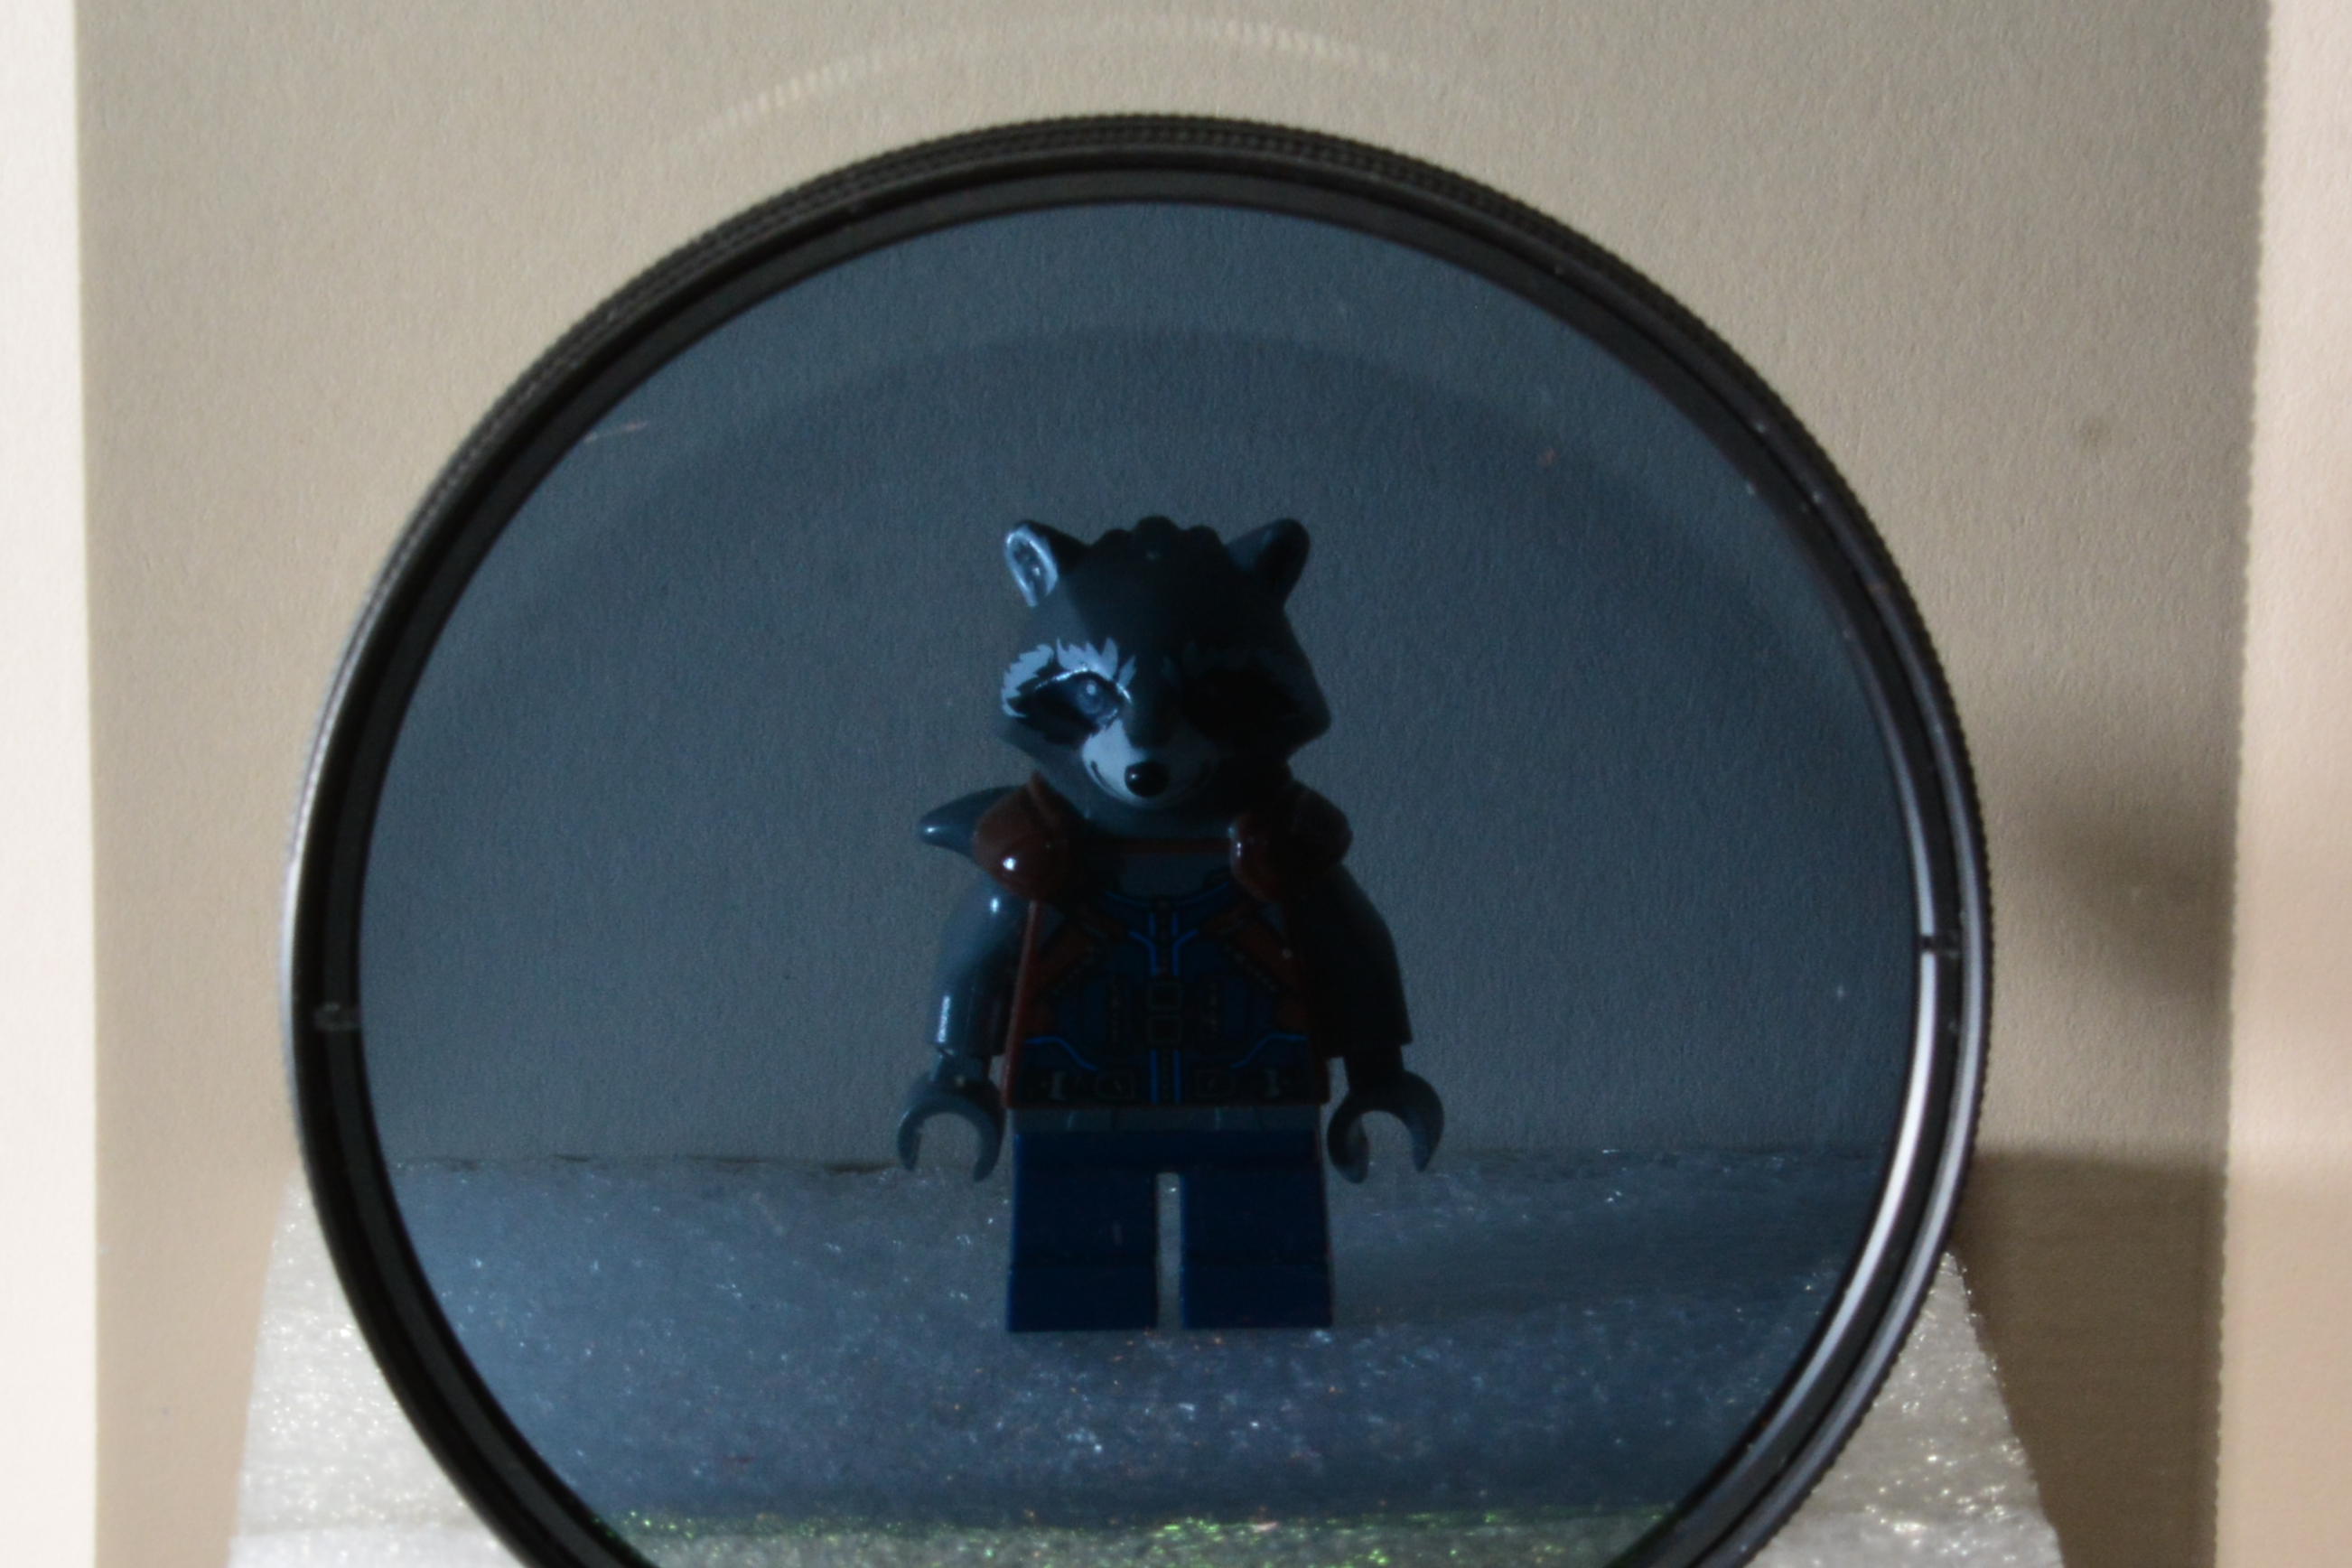
\includegraphics[width=7truecm]{slike/03_vrstnired2.JPG}
\caption{Učinek vpliva vrstnega reda cirkularnega in linearnega polarizatorja.
Na levi sliki je spredaj linearni polarizator in za njim cirkularni, na desni sliki
je vrstni red obrnjen in svetloba je prepuščena.}
\label{fig:03_VrstniRed}
\end{figure}
\end{example}

\section{Valovna enačba v prevodni snovi}
\label{section:35}
Obravnavajmo za konec še valovno enačbo v prevodni snovi. Snov naj
bo homogena, izotropna in nenabita ($\varrho_e = 0$). Izhajamo\index{Valovna enačba!{v prevodniku}|see{Telegrafska enačba}}
iz Maxwellovih enačb (enačbe~\ref{eq:Maxwell1}--\ref{eq:Maxwell4}) in zveze:
\begin{equation}
\mathbf{j}_e = \sigma \mathbf{E},
\label{eq:03_65}
\end{equation}
ki povezuje gostoto električnega toka $\mathbf{j}_e $ in jakost 
električnega polja $\mathbf{E}$. Sorazmernostni faktor, ki predstavlja\index{Električna prevodnost}
električno prevodnost, smo označili s $\sigma$. Tipična vrednost
za kovine je $\sigma > 10^6/\si{\ohm\m}$ in za izolatorje 
$\sigma < 10^{-6}/\si{\ohm\m}$. 
Električne tokove moramo upoštevati pri zapisu Amp\`{e}rovega zakona 
(enačba~\ref{eq:Maxwell1}):
\begin{equation}
\nabla\times\mathbf{H} =\frac{\partial\mathbf{D}}{\partial t}+\mathbf{j}_e = 
\varepsilon \varepsilon_0 \frac{\partial\mathbf{E}}{\partial t}+\sigma \mathbf{E}.
\label{eq:03_66}
\end{equation}
Izhajamo iz Faradayevega zakona (enačba~\ref{eq:Maxwell2}) in na njem izvedemo operacijo rotorja:
\begin{equation}
\nabla \times \left( \nabla \times  \mathbf{E}\right) = -\nabla\times \left(
\frac{\partial \mathbf{B}}{\partial t}\right) = - \mu \mu_0 \frac{\partial }{\partial t}
\left( \nabla \times \mathbf{H}\right)\!\!.
\label{eq:03_67}
\end{equation}
Vstavimo enačbo~(\ref{eq:03_66}) in dobimo:
\begin{equation}
\nabla \times \left( \nabla \times  \mathbf{E}\right) =
 -\mu \mu_0 \frac{\partial }{\partial t}
\left( \varepsilon \varepsilon_0 \frac{\partial\mathbf{E}}{\partial t}\right)-
\mu \mu_0 \frac{\partial }{\partial t}\left(\sigma \mathbf{E} \right)\!\!.
\label{eq:03_671}
\end{equation}
Upoštevamo še enačbo~(\ref{eq:03_02}) in dobimo zvezo:
\boxeq{eq:telegrafska}{
\nabla^2\mathbf{E} =  \mu \mu_0\varepsilon \varepsilon_0 \frac{\partial^2\mathbf{E}}{\partial t^2}
+ \mu \mu_0 \sigma \frac{\partial \mathbf{E}}{\partial t}.
}
Zapisano enačbo imenujemo telegrafska enačba. Podobno izpeljemo tudi telegrafsko enačbo
za gostoto magnetnega polja $\mathbf{B}$.\index{Telegrafska enačba}

Ker v telegrafski enačbi nastopa prvi odvod po času, po analogiji z mehanskimi
sistemi pričakujemo, da se valovanje v snovi duši oziroma slabi (atenuira). 
Rešitev zato iščemo v obliki ravnega valovanja:
\begin{equation}
\mathbf{E}(\mathbf{r},t) = \mathbf{E}_0 e^{i\mathbf{k}\cdot \mathbf{r} - i\omega t},
\label{eq:03_68}
\end{equation}
pri čemer dopuščamo možnost kompleksnega valovnega vektorja,\index{Valovni vektor!kompleksni} katerega imaginarni del
bo opisoval pojemanje amplitude. Ko nastavek (enačba~\ref{eq:03_68})
vstavimo v telegrafsko enačbo (enačba~\ref{eq:telegrafska}), dobimo:
\begin{equation}
-k^2 \mathbf{E} = \mu \mu_0\varepsilon \varepsilon_0 \left (-\omega^2 \mathbf{E}\right)
+ \mu \mu_0 \sigma \left(-i \omega\right)\mathbf{E}.
\label{eq:03_69}
\end{equation}
Sledi:
\begin{equation}
k^2 = \mu \mu_0\varepsilon \varepsilon_0 \omega^2 + i \mu \mu_0 \sigma\omega = 
\frac{\omega^2}{c_0^2} \varepsilon \mu  + i \frac{\omega^2}{c_0^2}\frac{\sigma \mu}{\varepsilon_0\omega}.
\label{eq:03_70}
\end{equation}
Vstavimo valovno število v vakuumu $k_0 = \omega/c_0$ in dobimo:
\begin{equation}
k^2 = k_0^2 \left( \varepsilon \mu + i \frac{\sigma \mu}{\varepsilon_0\omega} 
\right)\!\!.
\label{eq:03_71}
\end{equation}
Vpeljemo kompleksni lomni količnik $\mathcal{N}$, tako da velja:\index{Lomni količnik!kompleksni}
\boxeq{eq:nkompleks}{
k = k_0 \mathcal{N}.
}
Pri tem je:
\boxeq{eq:nkompleks2}{
\mathcal{N}^2 = \varepsilon \mu + i \frac{\sigma \mu}{\varepsilon_0\omega}.
}
Kompleksni lomni količnik $\mathcal{N}$ zapišemo kot vsoto realnega $n'$ in imaginarnega
dela $n''$:
\begin{equation}
\mathcal{N}^2 = (n'+in'')^2 = n'^2 -n''^2 + 2i n'n''.
\label{eq:03_72}
\end{equation}
Označimo realni del $\mathcal{N}^2$ (enačba~\ref{eq:nkompleks2})
z $x = \varepsilon \mu$ in imaginarni del z $y = \sigma \mu/\varepsilon_0\omega$.  
Rešujemo torej enačbo:
\begin{equation}
x + iy = n'^2 -n''^2 + 2i n'n''.
\label{eq:03_72a}
\end{equation}
Ločimo realni del:
\begin{equation}
x = n'^2 -n''^2
\label{eq:03_73}
\end{equation}
in imaginarni del:
\begin{equation}
y = 2n'n''.
\label{eq:03_74}
\end{equation}
Izrazimo $n''$ iz druge enačbe in ga vstavimo v prvo. Dobimo kvadratno enačbo:
\begin{equation}
n'^2-(y/2n')^2 = x
\label{eq:03_75}
\end{equation}
z rešitvijo:
\begin{equation}
n'^2 = \left(x + \sqrt{x^2+y^2}\right)/2.
\label{eq:03_76}
\end{equation}
Pri tem smo se omejili na rešitev s pozitivnim predznakom, saj je negativen predznak
za navadne snovi nesmiseln. Iz enačbe~(\ref{eq:03_73}) izračunamo še imaginarni del, 
ki je enak:
\begin{equation}
n''^2 = \left(-x + \sqrt{x^2+y^2}\right)/2.
\label{eq:03_77}
\end{equation}
Vstavimo izraza za $x$ in $y$ in dobimo:
\begin{equation}
n'^2 = \frac{1}{2}\left(\varepsilon \mu + \sqrt{(\varepsilon \mu)^2 + 
\left(\frac{\sigma \mu}{\varepsilon_0\omega}\right)^2}\right)
\label{eq:03_78}
\end{equation}
in
\begin{equation}
n''^2 = \frac{1}{2}\left(-\varepsilon \mu + \sqrt{(\varepsilon \mu)^2 + 
\left(\frac{\sigma \mu}{\varepsilon_0\omega}\right)^2}\right)\!\!.
\label{eq:03_79}
\end{equation}
Pogosto nas zanimajo nemagnetne snovi, v katerih je $\mu=1$. V takih
snoveh se kvadrat realnega dela lomnega količnika poenostavi v :
\begin{equation}
n'^2 = \frac{1}{2}\left(\varepsilon + \sqrt{\varepsilon^2 + 
\left(\frac{\sigma}{\varepsilon_0\omega}\right)^2}\right)\!\!,
\label{eq:03_80}
\end{equation}
kvadrat imaginarnega dela pa v:
\begin{equation}
n''^2 = \frac{1}{2}\left(-\varepsilon + \sqrt{\varepsilon^2 + 
\left(\frac{\sigma}{\varepsilon_0\omega}\right)^2}\right)\!\!.
\label{eq:03_81}
\end{equation}
Vstavimo zdaj izračunani lomni količnik v nastavek za jakost električnega polja 
(enačba~\ref{eq:03_68}) in poglejmo
primer, ko se svetloba širi v smeri $z$. Dobimo:
\begin{equation}
\mathbf{E} = \mathbf{E}_0 e^{ik_0\mathcal{N}z - i\omega t} = 
\mathbf{E}_0 e^{ik_0 n'z - i\omega t} \cdot e^{-k_0n''z}.
\label{eq:03_82}
\end{equation}
Zadnji člen opisuje eksponentno pojemanje amplitude polja z globino $z$ in ga pogosto
pišemo kot $\exp(-\kappa z)$, pri čemer je $\kappa = k_0 n''$.

V kovinah je prevodnost zelo velika in velja:
\begin{equation}
\frac{\sigma}{\omega\varepsilon_0} \gg \varepsilon.
\label{eq:03_83}
\end{equation}
Potem lahko imaginarni del lomnega količnika zapišemo kot:
\begin{equation}
n'' \approx \sqrt{\frac{\sigma}{2 \omega \varepsilon_0}}.
\label{eq:03_84}
\end{equation}
Parameter $\kappa$ je:
\begin{equation}
\kappa = k_0 n'' = \frac{\omega}{c_0} \sqrt{\frac{\sigma}{2 \omega \varepsilon_0}} = \sqrt{\frac{\mu_0 \omega \sigma}{2}}.
\label{eq:03_85}
\end{equation}
Nazornejše je vpeljati vdorno globino:\index{Vdorna globina}
\begin{equation}
d = \kappa^{-1} = \sqrt{\frac{2}{\mu_0 \omega \sigma}},
\label{eq:03_86}
\end{equation}
ki predstavlja karakteristično globino pojemanja električne poljske jakosti.
V kovinah je zaradi velike prevodnosti vdorna globina zelo majhna. Večina elektromagnetnega
valovanja oziroma izmeničnega toka zato teče po površini prevodnih snovi. Ta pojav poznamo pod imenom
kožni pojav.

\begin{example}{\bf Vdorna globina v bakru.}
Specifična upornost bakra je $\xi = 0,017~\si{\ohm\,\milli\metre^2/\metre}$ in 
prevodnost $\sigma = 1/\xi = 58 \times 10^6/\si{\ohm\metre}$. 
Vdorna globina je odvisna od frekvence elektro\-mag\-net\-nega valovanja, 
zato izračunajmo nekaj primerov: 
\begin{center}
\begin{tabular}{|c|c|}
\hline
$\nu~[\si{Hz}]$ & $d~[\si{nm}]$\\ \hline
50 & $\approx 10~\si{mm}$\\ \hline
$10^6$ & $\approx 100~\si{\micro\metre}$\\ \hline
$10^{10}$ & $\approx 1~\si{\micro\metre}$\\ \hline
$10^{15}$ & $\approx 3~\si{\nano\metre}$\\ \hline
\end{tabular}
\end{center}

Vdorna globina za vidno svetlobo je v bakru torej nekaj nanometrov. 
Izredno kratka vdorna globina v kovinah predstavlja velik problem pri izdelavi prozornih elektrod, 
ki jih potrebujemo na primer za izdelavo sončnih celic
ali tekočekristalnih zaslonov. Zato za ta namen navadno uporabljamo
kovine z razmeroma majhno prevodnostjo (npr. indijev 
kositrov oksid, ITO) in veliko vdorno globino. Debelina plasti, ki
jo nanesemo na steklo in ki še prepušča večino vpadne svetlobe, je 
v takih kovinah razmeroma velika, tipično 
okoli $100~\si{nm}$. 
\end{example}

\chapterimage{04_Odboj.jpg} % Chapter heading image

\chapter{Odboj in lom}
Dva izmed najosnovnejših optičnih pojavov sta odboj in lom valovanja na meji med 
dvema snovema. V tem poglavju bomo podrobneje spoznali, kako se svetloba odbije in lomi ter
kako se pri tem spremenita amplituda in faza valovanja. Opisali bomo totalni odboj,
vpeljali Brewstrov kot in na koncu spoznali še odboj svetlobe na meji s kovino.

\section{Robni pogoji na meji dveh dielektrikov}\index{Robni pogoji}
Že geometrijska optika, ki temelji na Fermatovem teoremu, pove, kako se svetloba na 
meji med dvema snovema odbija in lomi. Odbojni kot je enak vpadnemu (enačba~\ref{eq:odbojnizakon}), 
smer lomljenega žarka pa je odvisna od lomnih količnikov snovi (enačba~\ref{eq:lomnizakon}). 
Vendar geometrijska optika ne pove ničesar o amplitudah in fazah valovanj.
Za to potrebujemo valovno obravnavo svetlobe. 

Izhajamo iz Maxwellovih enačb (enačbe~\ref{eq:Maxwell1}--\ref{eq:Maxwell4}), ki 
opisujejo elektromagnetno valovanje v snovi. Za obravnavo prehoda
skozi mejo dveh snovi potrebujemo še ustrezne robne pogoje. Zapišimo jih
za mejo med snovema z lomnima količnikoma
$n_1$ in $n_2$. Na meji naj ne bo električnih tokov ali površinskih nabojev. 
V prvi snovi naj bo gostota električnega polja enaka $\mathbf{D}_1$ in v drugi 
$\mathbf{D}_2$.

Zapišimo Gaussov zakon (enačba~\ref{eq:Maxwell3}) v integralni obliki:\index{Gaussov zakon}
\begin{equation}
\oint \mathbf{D}\cdot d\mathbf{S} = 0.
\label{eq:04_01}
\end{equation}
Sklenjena ploskev, po kateri integriramo, naj bo kvader z dvema stranicama
vzporednima mejni ploskvi (slika~\ref{fig:04_RP}\,a). 
Ko gre višina kvadra $h \to 0$, ostaneta le še dva prispevka k integralu, to sta
skalarna produkta na zgornji
in spodnji ploskvi:
\begin{equation}
\mathbf{D}_1 \cdot \mathbf{s}_0\, S+ \mathbf{D}_2 \cdot (-\mathbf{s}_0)\,S = 0,
\label{eq:04_02}
\end{equation}
pri čemer vektor $\mathbf{s}_0 $ opisuje normalo na ploskev kvadra in hkrati na mejno ravnino, $S$ pa je 
ploščina posamezne ploskve.
\begin{figure}[!ht]
\centering
\def\svgwidth{130truemm} 
\input{slike/04_RP.pdf_tex}
\caption{K izpeljavi robnih pogojev na meji med dvema snovema. Prvi robni pogoj je ohranitev
pravokotne komponente $\mathbf{D}$ (a), drugi pa ohranitev tangentne komponente 
$\mathbf{E}$ (b).}
\label{fig:04_RP}
\end{figure}

Sledi:\index{Robni pogoji!{gostota električnega polja}}
\boxeq{eq:RPD}{
\left( \mathbf{D}_2-\mathbf{D}_1 \right) \cdot \mathbf{s}_0 = 0 \qquad \mathrm{oziroma} \qquad
D_{1\perp} = D_{2\perp}.
}
Pri prehodu skozi mejo dveh snovi se ohranja normalna komponenta gostote
električnega polja. Povsem enak račun naredimo za gostoto magnetnega polja, 
če izhajamo iz enačbe:
\begin{equation}
\oint \mathbf{B}\cdot d\mathbf{S} = 0.
\label{eq:04_03}
\end{equation}
Pri prehodu skozi mejo dveh snovi se tako ohranja normalna komponenta
gostote magnetnega polja:\index{Robni pogoji!{gostota magnetnega polja}}
\boxeq{eq:RPB}{
\left( \mathbf{B}_2-\mathbf{B}_1 \right) \cdot \mathbf{s}_0 = 0 \qquad 
\mathrm{oziroma} \qquad B_{1\perp} = B_{2\perp}.
}

Naredimo zdaj še pravokotno zanko, ki leži v ravnini, pravokotni na mejo dveh 
snovi (slika~\ref{fig:04_RP}\,b). Zanko izberemo v ravnini, ki jo določata vektorja normale na 
mejo $\mathbf{s}_0$ in jakosti električnega polja $\mathbf{E}$. 
Zapišemo Faradayev zakon (enačba~\ref{eq:Maxwell2}) v integralni obliki, pri 
čemer integriramo po sklenjeni zanki:\index{Faradayev zakon}
\begin{equation}
\oint \mathbf{E}\cdot d\mathbf{l} = - \frac{\partial}{\partial t}\int \mathbf{B}\cdot d\mathbf{S}.
\label{eq:04_04}
\end{equation}
Višino zanke naredimo kar se da majhno ($h \to 0$), zato na levi strani ostaneta le še 
integrala po zgornji in spodnji stranici, integral na desni strani pa gre proti 0. Dobimo:
\begin{equation}
\mathbf{E}_1 \cdot d\mathbf{l} - \mathbf{E}_2 \cdot d\mathbf{l} = 0.
\label{eq:04_05}
\end{equation}
Ohranja se torej projekcija vektorja jakosti električnega polja na mejo med snovema. 
Ker je vektor $d\mathbf{l}$ vzporeden z mejo, vektor $\mathbf{s}_0$ pa 
pravokoten nanjo, lahko zgornji izraz zapišemo kot:\index{Robni pogoji!{jakost električnega polja}}
\boxeq{eq:RPE}{
\left( \mathbf{E}_2-\mathbf{E}_1 \right) \times \mathbf{s}_0 = 0 \qquad \mathrm{oziroma} \qquad
E_{1 \myparallel} = E_{2 \myparallel}.
}
Podobno izpeljemo tudi robni pogoj za ohranitev tangentne komponente
jakosti magnetnega polja:\index{Robni pogoji!{jakost magnetnega polja}}
\boxeq{eq:RPH}{
\left( \mathbf{H}_2-\mathbf{H}_1 \right) \times \mathbf{s}_0 = 0 \qquad \mathrm{oziroma} \qquad
H_{1\myparallel} = H_{2\myparallel}.
}
Tako smo zapisali štiri robne pogoje za ohranitev komponent gostote in jakosti električnega
in magnetnega polja na meji med dvema snovema (slika~\ref{fig:04_RP2}). 
\begin{figure}[!ht]
\centering
\def\svgwidth{80truemm} 
\input{slike/04_RP2.pdf_tex}
\caption{Na mejah med snovmi se ohranjata normalna komponenta $\mathbf{D}_\perp$ in tangentna komponenta 
$\mathbf{E}_\myparallel$.}
\label{fig:04_RP2}
\end{figure}

\section{Odbojni in lomni zakon}
Zamislimo si ravno potujoče sinusno elektromagnetno valovanje, 
ki vpada na mejo med dvema snovema z lomnima količnikoma $n_1$ in $n_2$. 
Vemo, da se vpadno valovanje razdeli na odbito in prepuščeno (lomljeno) 
valovanje. Zanima nas, kakšne lastnosti imata odbito in prepuščeno 
valovanje, da zadostita robnim pogojem (enačbe~\ref{eq:RPD}, \ref{eq:RPB}, 
\ref{eq:RPE} in \ref{eq:RPH}). 

Naj žarek svetlobe vpada na mejno ravnino pod kotom $\alpha$ glede na normalo na mejo (glej
sliko~\ref{fig:04_lom}). Njegov valovni vektor naj bo $\mathbf{k}_i$, 
krožna frekvenca $\omega_i$, faza $\delta_i$ in amplituda $\mathbf{E}_{0i}$. 
Pripadajoče valovno število
je $k_i = \omega_i n_1/c_0$. Vpadno valovanje na splošno zapišemo kot:
\begin{equation}
\mathbf{E}_i = \mathbf{E}_{0i} e^{i\mathbf{k}_i\cdot \mathbf{r} - i \omega_i t + i \delta_i}.
\label{eq:04_06}
\end{equation}
Odbito valovanje zapišemo z valovnim vektorjem $\mathbf{k}_r$, 
krožno frekvenco $\omega_r$, fazo $\delta_r$ in amplitudo $\mathbf{E}_{0r}$: 
\begin{equation}
\mathbf{E}_r = \mathbf{E}_{0r} e^{i\mathbf{k}_r\cdot \mathbf{r} - i \omega_r t + i \delta_r}.
\label{eq:04_07}
\end{equation}
Podobno prepuščeno valovanje določajo valovni vektor $\mathbf{k}_t$, 
krožna frekvenca $\omega_t$, faza $\delta_t$ in amplituda $\mathbf{E}_{0t}$:
\begin{equation}
\mathbf{E}_t = \mathbf{E}_{0t} e^{i\mathbf{k}_t\cdot \mathbf{r} - i \omega_t t + i \delta_t}.
\label{eq:04_08}
\end{equation}
\begin{figure}[!ht]
\centering
\def\svgwidth{130truemm} 
\input{slike/04_lom.pdf_tex}
\caption{K izpeljavi odboja in loma na meji dveh snovi (a). Pri odboju in lomu
se ohranja komponenta valovnega vektorja, ki je vzporedna z mejno ploskvijo (b).}
\label{fig:04_lom}
\end{figure}

Mejo med snovema postavimo v ravnino $z=0$. Iz robnega pogoja za ohranitev tangentne
komponente vektorja $\mathbf{E}$ (enačba~\ref{eq:RPE}) dobimo zvezo:
\begin{equation}
\mathbf{E}_{i\myparallel} + \mathbf{E}_{r\myparallel} = \mathbf{E}_{t\myparallel},
\label{eq:04_09}
\end{equation}
oziroma izpisano:
\begin{equation}
\mathbf{E}_{0i\myparallel} e^{ik_{ix}x+ik_{iy}y - i \omega_i t + i \delta_i}+
\mathbf{E}_{0r\myparallel} e^{ik_{rx}x+ik_{ry}y - i \omega_r t + i \delta_r} =
\mathbf{E}_{0t\myparallel} e^{ik_{tx}x+ik_{ty}y - i \omega_t t + i \delta_t}.
\label{eq:04_10}
\end{equation}
Zapisana zveza mora veljati 
ob vseh časih $t$ in za vse vrednosti $x$ in $y$. Vzemimo najprej $x=y=0$ in $t=0$. 
Od tod sledi, da so vse faze enake in $\delta_i = \delta_r = \delta_t$.
Drugi pogoj poglejmo pri $x=y=0$ in poljubnem času $t>0$. Robni pogoj 
je izpolnjen le v primeru, da velja 
\boxeq{eq:omegakonst}{
\omega_i =
\omega_r = \omega_t,
}
kar pomeni, da se krožna frekvenca valovanja pri odboju in lomu ohranja. 

Obravnavajmo zdaj primer $t=0$ pri poljubnem paru $x,y$ oziroma vektorju $\mathbf{r}$
v mejni ravnini. Da bo robni pogoj izpolnjen za vsak $\mathbf{r}$,
mora veljati:
\begin{equation}
\mathbf{k}_i\cdot \mathbf{r} = \mathbf{k}_r\cdot \mathbf{r} = 
\mathbf{k}_t\cdot \mathbf{r} = \mathrm{konst.}
\label{eq:04_11}
\end{equation}
Iz tega sledi pomembna ugotovitev, da ležijo valovni vektorji vpadnega, odbitega
in lomljenega valovanja vedno v eni ravnini. Imenujemo jo vpadna ravnina.\index{Vpadna ravnina}
Navadno izberemo, da je vpadna ravnina ravnina $xz$. Potem zapišemo 
valovne vektorje vpadne, odbite in prepuščene svetlobe kot:\index{Valovni vektor}
\begin{align}
\mathbf{k}_i  &= \left( \sin\alpha, 0, \cos \alpha\right) \frac{\omega}{c_0} n_1, \label{eq:04_12}\\
\mathbf{k}_r  &= \left( \sin\tilde{\alpha}, 0, -\cos \tilde{\alpha}\right) 
\frac{\omega}{c_0} n_1\label{eq:04_13} \qquad \mathrm{in}\\
\mathbf{k}_t  &= \left( \sin\beta, 0, \cos \beta\right) \frac{\omega}{c_0} n_2.\label{eq:04_14}
\end{align}
Poleg vpadnega kota $\alpha$ smo vpeljali še odbojni kot $\tilde{\alpha}$ in lomni
kot $\beta$.\index{Lomni kot}\index{Vpadni kot}

Iz enačbe~(\ref{eq:04_11}) sledi, da so projekcije vseh treh valovnih vektorjev na mejno
ravnino enake (slika~\ref{fig:04_lom}\,b) in velja:
\begin{equation}
k_{ix} = k_{rx} = k_{tx}.
\label{eq:04_15}
\end{equation}
Najprej poglejmo prvo enakost ($k_{ix} = k_{rx}$). Vstavimo komponenti valovnih
vektorjev (enačbi~\ref{eq:04_12} in \ref{eq:04_13}) in dobimo:
\begin{equation}
\frac{\omega}{c_0} n_1 \sin \alpha  =  \frac{\omega}{c_0} n_1 \sin\tilde{\alpha}.
\label{eq:04_16}
\end{equation}
Od tod sledi odbojni zakon, ki pravi, da je odbojni kot enak vpadnemu:\index{Odbojni zakon}
\boxeq{eq:odbojni}{
\tilde\alpha = \alpha.
}

Poglejmo zdaj še drugo enakost ($k_{ix} = k_{tx}$). Vstavimo komponenti
valovnih vektorjev (enačbi~\ref{eq:04_12} in \ref{eq:04_14}) in dobimo:\index{Lomni zakon}
\begin{equation}
\frac{\omega}{c_0} n_1 \sin \alpha  = \frac{\omega}{c_0} n_2\sin\beta.
\label{eq:04_17}
\end{equation}
Od tu sledi lomni zakon:
\boxeq{eq:04_18}{
n_1 \sin \alpha = n_2 \sin \beta.
}

Z odbojnim in lomnim zakonom smo izpolnili ujemanje faz v enačbi~(\ref{eq:04_10}). 
Hribi in doline vpadnega, odbitega in prepuščenega valovanja vzdolž meje 
potujejo enako hitro. Dodatno informacijo o valovanju dobimo, če
uskladimo še amplitude jakosti električnih polj. Preden izpeljemo
zveze, ki povezujejo razmerja med amplitudami, vpeljimo koordinatni sistem
in se dogovorimo o oznaki polarizacij.

Za obravnavo izberemo dve ortogonalni linearni polarizaciji, saj lahko
poljubno polarizacijo sestavimo kot kombinacijo teh dveh.
Mejna ravnina naj bo še naprej ravnina $xy$, os $z$ pa naj bo obrnjena navzdol. 
V prvem primeru naj bo jakost električnega polja
vpadne, odbite in prepuščene svetlobe vzporedna z osjo $y$ in torej pravokotna
na vpadno ravnino (slika~\ref{fig:04_tetm}\,a). 
Tako valovanje imenujemo transverzalno električno (TE) valovanje.\index{Polarizacija!{transverzalna električna}}
\index{Polarizacija!TE|see {transverzalna električna}}
V literaturi zasledimo tudi oznaki $s$ (kot {\it senkrecht}, pravokotno) ali $\sigma$.

\begin{figure}[ht]
\centering
\def\svgwidth{140truemm} 
\input{slike/04_tetm.pdf_tex}
\caption{V primeru transverzalne električne (TE) polarizacije leži jakost
električnega polja pravokotno na vpadno ravnino (a),
pri transverzalni magnetni (TM) polarizaciji pa leži jakost električnega
polja v vpadni ravnini (b). Jakost električnega polja je označena z rdečimi
puščicami, gostota magnetnega polja pa z modrimi.}
\label{fig:04_tetm}
\end{figure}

V drugem primeru ležijo jakosti električnega polja v 
vpadni ravnini (slika~\ref{fig:04_tetm}\,b), gostote magnetnega polja 
pa so pravokotne nanjo. To polarizacijo zato poimenujemo 
transverzalna magnetna (TM) polarizacija. Uporabljajo se tudi oznake
$p$ (kot {\it parallel}, vzporedno) ali $\pi$. 
Omenjena primera bomo obravnavali ločeno, začenši s TE polarizacijo. V 
obeh primerih se bomo omejili na izotropne in nemagnetne snovi ($\mu=1$).
\index{Polarizacija!{transverzalna magnetna}}
\index{Polarizacija!TM|see {transverzalna magnetna}}

\section{Fresnelove enačbe za transverzalno električno valovanje}
Osnovna zahteva na meji med dvema snovema je izpolnjevanje robnih\index{Polarizacija!{transverzalna električna}}
pogojev, po katerih se na meji ohranja tangentna komponenta jakosti električnega
polja. Ker so pri TE polariziranem valovanju 
vpadna, odbita in prepuščena jakost polja vzporedne z osjo $y$, velja preprosta zveza:
\begin{equation}
E_{0i} + E_{0r}= E_{0t}.
\label{eq:04_19}
\end{equation}
Pri tem smo upoštevali, da je polje v prvi snovi vsota polja vpadnega in odbitega
valovanja, v drugi snovi pa je samo prepuščeno valovanje. Drugi robni pogoj, ki zahteva
ohranitev normalne komponente gostote električnega polja (enačba~\ref{eq:RPD}) je 
vedno izpolnjen, saj je ta komponenta v obeh snoveh identično enaka nič. 

Tretji robni pogoj (enačba~\ref{eq:RPH}) zahteva
ohranitev tangentne komponente jakosti magnetnega polja. Ob privzetku, da
sta snovi nemagnetni, dobimo:
\begin{equation}
-B_{0i}\cos \alpha + B_{0r}\cos \alpha = -B_{0t}\cos \beta.
\label{eq:04_20}
\end{equation}
Upoštevajoč zvezo med amplitudama električnega in magnetnega 
polja $E_0 = B_0 c = B_0 c_0/n$  (enačba~\ref{eq:EBc}) zapišemo robni pogoj kot:
\begin{equation}
- E_{0i}n_1\cos \alpha + E_{0r}n_1\cos \alpha = - E_{0t}n_2\cos \beta.
\label{eq:04_21}
\end{equation} 
Hiter račun pokaže, da je četrti robni pogoj, ki predstavlja ohranitev 
normalne komponente gostote magnetnega polja (enačba~\ref{eq:RPB}), 
ekvivalenten prvemu pogoju (enačba~\ref{eq:04_19}) in ne da nove informacije. 

Iz robnih
pogojev tako dobimo dve neodvisni enačbi (enačbi~\ref{eq:04_19} in \ref{eq:04_21}), 
ki povezujeta tri neznanke: $E_{0i}$, $E_{0r}$ in $E_{0t}$. Navadno izrazimo amplitudi
odbitega in prepuščenega valovanja z amplitudo vpadnega valovanja. Izraza, s katerima določimo 
relativni amplitudi odbite in prepuščene svetlobe, imenujemo Fresnelovi enačbi. Zapišimo ju.

Pomnožimo enačbo~(\ref{eq:04_19}) z $n_2 \cos \beta$ in ji prištejmo
enačbo~(\ref{eq:04_21}). Dobimo:
\begin{equation}
\left( n_2 \cos \beta-n_1 \cos \alpha\right) E_{0i} + 
\left( n_2 \cos \beta+n_1 \cos \alpha\right) E_{0r} = 0.
\label{eq:04_26}
\end{equation}
Vpeljemo amplitudno odbojnost $r = E_{0r}/E_{0i}$\index{Amplitudna odbojnost!{TE}}
kot razmerje amplitud jakosti električnega polja odbitega in vpadnega valovanja.\index{Fresnelove enačbe}
Iz enačbe~(\ref{eq:04_26}) sledi:
\boxeq{eq:TEr}{
r_\mathrm{TE}  = \frac{n_1 \cos \alpha - n_2 \cos \beta}
{n_1 \cos \alpha + n_2 \cos \beta},
}
pri čemer $\alpha$ in $\beta$ označujeta vpadni in lomni kot. Fresnelovo enačbo za amplitudno odbojnost
$r$ z uporabo lomnega zakona (enačba~\ref{eq:04_18}) preoblikujemo:\index{Amplitudna prepustnost!{TE}}
\begin{equation}
r = \frac{\frac{n_1}{n_2} \cos \alpha - \cos \beta}{\frac{n_1}{n_2} \cos \alpha - \cos \beta} = 
\frac{\frac{\sin \beta}{\sin \alpha} \cos \alpha - \cos \beta}
{\frac{\sin \beta}{\sin \alpha} \cos \alpha - \cos \beta} = \frac{\sin \beta \cos \alpha -
\cos \beta \sin \alpha}{\sin \beta \cos \alpha + \cos \beta \sin \alpha} = 
-\frac{\sin (\alpha -\beta)}{\sin (\alpha + \beta)}.
\label{eq:04_27}
\end{equation}

Izračunajmo še amplitudno prepustnost $t = E_{0t}/E_{0i}$, ki jo vpeljemo
kot razmerje amplitud jakosti električnega polja prepuščenega in vpadnega valovanja. Izhajamo
iz prvega robnega pogoja (enačba~\ref{eq:04_19}) in zapišemo:
\begin{equation}
t = \frac{E_{0t}}{E_{0i}} = \frac{E_{0i} + E_{0r}}{E_{0i}} = 1+ r.
\label{eq:04_28}
\end{equation}
Fresnelova enačba za amplitudno prepustnost je tako:\index{Fresnelove enačbe}
\boxeq{eq:TEt}{
t_\mathrm{TE} = 1+r = \frac{2n_1\cos \alpha}{n_1 \cos \alpha + n_2 \cos \beta}.
}

\section{Fresnelove enačbe za transverzalno magnetno valovanje}
Izračun amplitudne odbojnosti in prepustnosti za\index{Polarizacija!{transverzalna magnetna}}
transverzalno magnetno polarizirano valovanje začnemo podobno kot za 
TE polarizirano valovanje, to je z ustreznimi robnimi pogoji. 
Na meji dveh snovi se ohranja tangentna 
komponenta jakosti magnetnega polja (enačba~\ref{eq:RPH}):
\begin{equation}
H_{0i} + H_{0r}= H_{0t}.
\label{eq:04_29}
\end{equation}
Privzamemo, da so snovi nemagnetne in velja: $\mu_1 = \mu_2 = 1$. Potem enačbo
prepišemo v:
\begin{equation}
B_{0i} + B_{0r}= B_{0t}.
\label{eq:04_30}
\end{equation}
Iz zveze med amplitudama električnega in magnetnega polja (enačba~\ref{eq:EBc})
dobimo:
\begin{equation}
E_{0i}n_1 + E_{0r}n_1= E_{0t}n_2.
\label{eq:04_31}
\end{equation}
Drugi robni pogoj (enačba~\ref{eq:RPB}), ki pravi, da se ob prehodu v drugo snov ohranja
pravokotna komponenta gostote magnetnega polja, je prav tako izpolnjen, saj je $B_{\perp}=0$. 
Iz ohranitve tangentne komponente jakosti
električnega polja (enačba~\ref{eq:RPE}) sledi:
\begin{equation}
E_{0i} \cos \alpha - E_{0r}\cos \alpha = E_{0t}\cos \beta.
\label{eq:04_32}
\end{equation}
Predznak jakosti električnega polja smo zapisali v skladu s sliko~\ref{fig:04_tetm}. 
Za vajo bi lahko zapisali še četrti robni pogoj, vendar tudi v tem primeru ne bi dobili nove informacije.

Ostaneta dve enačbi za tri neznanke in ponovno lahko
izrazimo amplitudi polja odbite in prepuščene svetlobe z amplitudo polja vpadne svetlobe. 
Enačbo (\ref{eq:04_31}) pomnožimo s $\cos \beta$, enačbo~(\ref{eq:04_32}) pa z $n_2$:
\begin{align}
E_{0i} n_1 \cos \beta + E_{0r} n_1 \cos \beta  &= E_{0t} n_2 \cos \beta \label{eq:04_35} \\
E_{0i} n_2 \cos \alpha - E_{0r} n_2 \cos \alpha &= E_{0t} n_2 \cos \beta\label{eq:04_36}.
\end{align}
Enačbi odštejemo in dobimo:
\begin{equation}
E_{0i} \left(n_1 \cos \beta - n_2 \cos \alpha \right) + E_{0r} \left(n_1 \cos \beta + 
n_2 \cos \alpha \right) = 0.
\label{eq:04_37}
\end{equation}
Od tod izračunamo amplitudno odbojnost $r = E_{0r}/E_{0i}$, ki je 
razmerje med odbito in vpadno amplitudo jakosti električnega polja. Dobimo Fresnelovo enačbo:\index{Amplitudna odbojnost!{TM}}\index{Fresnelove enačbe}
\boxeq{eq:TMr}{
r_\mathrm{TM} = \frac{n_2 \cos \alpha - n_1 \cos \beta}{n_2 \cos \alpha + n_1 \cos \beta}.
}
Tudi ta izraz lahko predelamo z upoštevanjem lomnega zakona:
\begin{equation}
r = \frac{\frac{n_2}{n_1} \cos \alpha - \cos \beta}{\frac{n_2}{n_1} \cos \alpha - \cos \beta} = 
\frac{\frac{\sin \alpha}{\sin \beta} \cos \alpha - \cos \beta}
{\frac{\sin \alpha}{\sin \beta} \cos \alpha - \cos \beta} = 
\frac{\sin \alpha \cos \alpha -\cos \beta \sin \beta}
{\sin \alpha \cos \alpha + \cos \beta \sin \beta}.
\label{eq:04_38}
\end{equation}
Izraz preoblikujemo z vpeljavo dvojnih kotov:
\begin{equation}
r = \frac{\sin(2\alpha) - \sin(2\beta)}{\sin(2\alpha) + \sin(2\beta)} = \frac{2\cos(\alpha+\beta )\sin(\alpha-\beta )}
{2\sin(\alpha+\beta )\cos(\alpha-\beta )}
\label{eq:04_39}
\end{equation}
in dobimo:
\begin{equation}
r =\frac{\tan(\alpha-\beta )}{\tan(\alpha+\beta )}.
\label{eq:04_40}
\end{equation}
Fresnelovo enačbo za amplitudno prepustnost $t = E_{0t}/E_{0i}$ 
dobimo iz enačbe~(\ref{eq:04_31}):\index{Fresnelove enačbe}\index{Amplitudna prepustnost!{TM}}
\boxeq{eq:TMt}{
t_\mathrm{TM} = \frac{n_1}{n_2}\left(1+r \right) = 
\frac{2 n_1 \cos \alpha}{n_2 \cos \alpha + n_1 \cos \beta}.
}

\begin{example}{\bf Amplitudna odbojnost in amplitudna prepustnost pri pravokotnem vpadu.} 
Izračunali smo amplitudni odbojnosti $r$ in amplitudni prepustnosti $t$ za obe med seboj 
pravokotni polarizaciji TE in TM. Poglejmo najprej najpreprostejši primer, pri katerem
svetloba vpada pravokotno na mejo snovi. V tem primeru so vpadni, odbojni in 
lomni kot enaki in $\alpha = \tilde{\alpha} = \beta = 0$. Za TE polarizirano valovanje dobimo:
\begin{equation}
r_{\mathrm{TE}} = \frac{n_1 -n_2}{n_1+n_2} \qquad \mathrm{in} \qquad
t_{\mathrm{TE}} = \frac{2n_1}{n_1+n_2},
\label{eq:04_42}
\end{equation}
za TM polarizirano valovanje pa:
\begin{equation}
r_{\mathrm{TM}} = \frac{n_2 -n_1}{n_2+n_1} \qquad \mathrm{in} \qquad
t_{\mathrm{TM}} = \frac{2n_1}{n_1+n_2}.
\label{eq:04_43}
\end{equation}
Ker je vpad pravokoten, pričakujemo enaka rezultata za obe polarizaciji, saj 
polarizacij pri pravokotnem vpadu ne moremo ločiti med seboj. Rezultata za
prepuščeno svetlobo sta res enaka, za odbito svetlobo pa se razlikujeta za predznak.
Vzrok za to navidezno neenakost je v začetni izbiri smeri polarizacije 
pri odboju (glej sliko~\ref{fig:04_tetm}).
Odbojnost je z upoštevanjem privzete smeri tako enaka za obe polarizaciji 
-- kar je seveda pravilno.
\end{example}

\section{Energijski tok pri odboju in lomu}
V poskusih nas navadno zanima energijski tok valovanja. Gostoto energijskega
toka na splošno zapišemo kot (enačba~\ref{eq:j}):\index{Gostota svetlobnega toka}
\begin{equation}
j = \frac{1}{2} \varepsilon_0E_0^2 c_0 n.
\label{eq:04_44}
\end{equation}
Odbojnost $\mathcal{R}$ vpeljemo kot razmerje med odbitim in vpadnim svetlobnim tokom oziroma
kot razmerje med gostotama energijskih
tokov odbite $j_r$ in vpadne svetlobe $j_i$:\index{Odbojnost}
\begin{equation}
\mathcal{R} = \frac{j_r}{j_i} = \frac{\frac{1}{2}\varepsilon_0 E_{0r}^2 c_0 n_1}
{\frac{1}{2}\varepsilon_0 E_{0i}^2 c_0 n_1} = \left(\frac{E_{0r}}{E_{0i}}\right)^2\!\!.
\label{eq:04_45}
\end{equation}
V razmerju jakosti električnega polja prepoznamo amplitudno odbojnost in zapišemo:
\boxeq{eq:TEMR}{
\mathcal{R} = |r|^2.
}

Izračunajmo še prepustnost $\mathcal{T}$, ki je razmerje med prepuščenim in vpadnim svetlobnim
tokom. To razmerje ni enako razmerju gostot svetlobnih tokov, saj se zaradi\index{Prepustnost}
spremenjene smeri valovanja spremeni velikost ploskve, skozi
katero se pretoči vpadni svetlobni tok $P$ (slika~\ref{fig:04_coscos}).
\begin{figure}[ht]
\centering
\def\svgwidth{60truemm} 
\input{slike/04_coscos.pdf_tex}
\caption{Pri prehodu skozi mejo se zaradi loma spremeni velikost
ploskve, skozi katero se pretaka vpadni svetlobni tok.}
\label{fig:04_coscos}
\end{figure}

Zapišemo: 
\begin{equation}
\mathcal{T} = \frac{P_t}{P_i} = \frac{j_t}{j_i}\frac{S\cos \beta}{S\cos \alpha} =
\frac{\frac{1}{2}\varepsilon_0 E_{0t}^2 c_0 n_2}
{\frac{1}{2}\varepsilon_0 E_{0i}^2 c_0 n_1} \frac{\cos\beta}{\cos\alpha}= 
\left(\frac{E_{0t}}{E_{0i}}\right)^2 \frac{n_2\cos\beta}{n_1\cos\alpha}.
\label{eq:04_46}
\end{equation}
Prepustnost je torej enaka:
\boxeq{eq:TEMT}{
\mathcal{T} = |t|^2 \frac{n_2\cos\beta}{n_1\cos\alpha}.
}

Kratek  račun pokaže, da med odbojnostjo $\mathcal{R}$ in prepustnostjo $\mathcal{T}$ velja zveza:
\boxeq{eq:TEMRT}{
\mathcal{R}+\mathcal{T} = 1.
}
Rezultat je seveda pričakovan, saj opisuje ohranitev energije. Pogosto je najpriročnejše
izračunati odbojnost, nato pa z uporabo enačbe~(\ref{eq:TEMRT}) še prepustnost. 

Opozorimo še enkrat, da je pri izračunu prepustnosti treba upoštevati tudi 
spremembo lomnega količnika in kota širjenja svetlobe, zato:
\begin{equation}
|r|^2+ |t|^2 \neq 1.
\label{eq:04_48}
\end{equation}

\begin{example}{\bf Odbojnost pri pravokotnem vpadu na steklo.} 
Izračunajmo, kolikšna je odbojnost svetlobe, ki vpada pod pravim kotom iz zraka na
steklo z lomnim količnikom $n_2=1,5$. Uporabimo enačbi~(\ref{eq:TEr}) in (\ref{eq:TEMR})
in dobimo:
\begin{equation}
\mathcal{R} = \left(\frac{n_1-n_2}{n_1+n_2}\right)^2 \approx~4~\%.
\label{eq:04_49}
\end{equation}
Ob pravokotnem vpadu na steklo se $4~\%$ svetlobe odbije, ostala 
svetloba je prepuščena. Če želimo izračunati odbojnost na stekleni plošči, 
moramo seveda upoštevati, da se svetloba odbija
na obeh mejah steklo/zrak -- prvič, ko vstopi v steklo, in drugič, ko iz stekla
izstopi.
\end{example}

\section{Prehod v optično gostejšo snov}
\label{chap:lomgost}\index{Lom!{v optično gostejšo snov}}
Najprej obravnavajmo prehajanje svetlobe iz snovi z manjšim lomnim
količnikom v snov z večjim lomni količnikom ($n_1<n_2$), na primer
iz zraka v vodo ali iz zraka v steklo. Uporabimo
Fresnelove enačbe in izračunajmo  odbojnosti in prepustnosti za obe polarizaciji. 

Začnimo z amplitudno odbojnostjo in amplitudno prepustnostjo za TE polarizacijo v odvisnosti
\index{Polarizacija!{transverzalna električna}}
od vpadnega kota (slika~\ref{fig:04_redte}\,a).\index{Amplitudna odbojnost!{TE}}\index{Amplitudna prepustnost!{TE}}
Iz enačbe~(\ref{eq:TEr}) sledi, da je amplitudna odbojnost $r_\mathrm{TE}$
za vse kote negativna. Njena velikost se zvezno spreminja od začetne vrednosti
pri pravokotnem vpadu do vrednosti $-1$, ko se vpadni kot približuje $90\si{\degree}$.
Negativni predznak pri kotu $\alpha =0$ pomeni, da se svetloba pri 
pravokotnem vpadu na optično gostejše sredstvo vedno odbije z nasprotno fazo, ne 
glede na njeno polarizacijo.\index{Faza pri odboju}

\begin{figure}[ht]
\centering
\def\svgwidth{140truemm} 
\input{slike/04_redte.pdf_tex}
\caption{Odvisnost amplitudne odbojnosti in amplitudne prepustnosti (a) ter odbojnosti in 
prepustnosti (b) za TE polarizirano valovanje v odvisnosti od vpadnega kota $\alpha$}
\label{fig:04_redte}
\end{figure}

Amplitudna prepustnost $t_\mathrm{TE}$, ki jo izračunamo kot $t=r+1$, je za vse
vpadne kote pozitivna in pojema od največje vrednosti pri pravokotnem vpadu
do vrednosti $0$, ko se vpadni kot približuje $90\si{\degree}$. 

Odbojnost $\mathcal{R}_\mathrm{TE}$, ki jo izračunamo kot kvadrat amplitudne odbojnosti,
je prikazana na sliki~\ref{fig:04_redte}\,b. Vrednost je po pričakovanju\index{Odbojnost}
vedno pozitivna in narašča od neke začetne vrednosti pri pravokotnem
vpadu do vrednosti $1$, ko se vpadni kot približuje $90\si{\degree}$. Prepustnost\index{Prepustnost}
$\mathcal{T}_\mathrm{TE}$ izračunamo po enačbi $\mathcal{T} = 1 -\mathcal{R}$. 
\begin{figure}[ht]
\centering
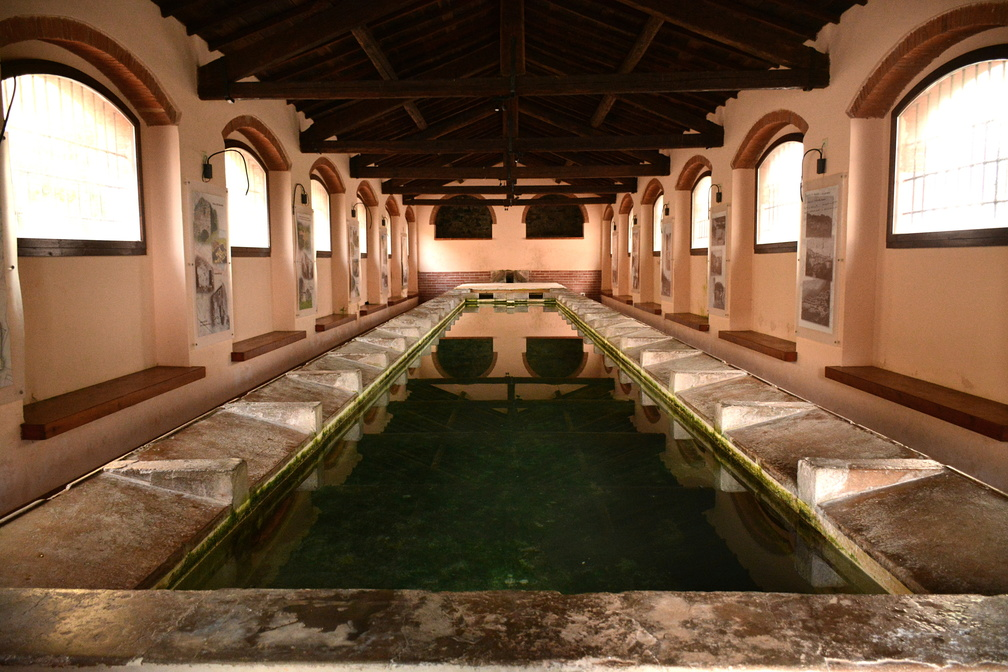
\includegraphics[width=7truecm]{slike/04_OdbojFoto.jpg}\hfill
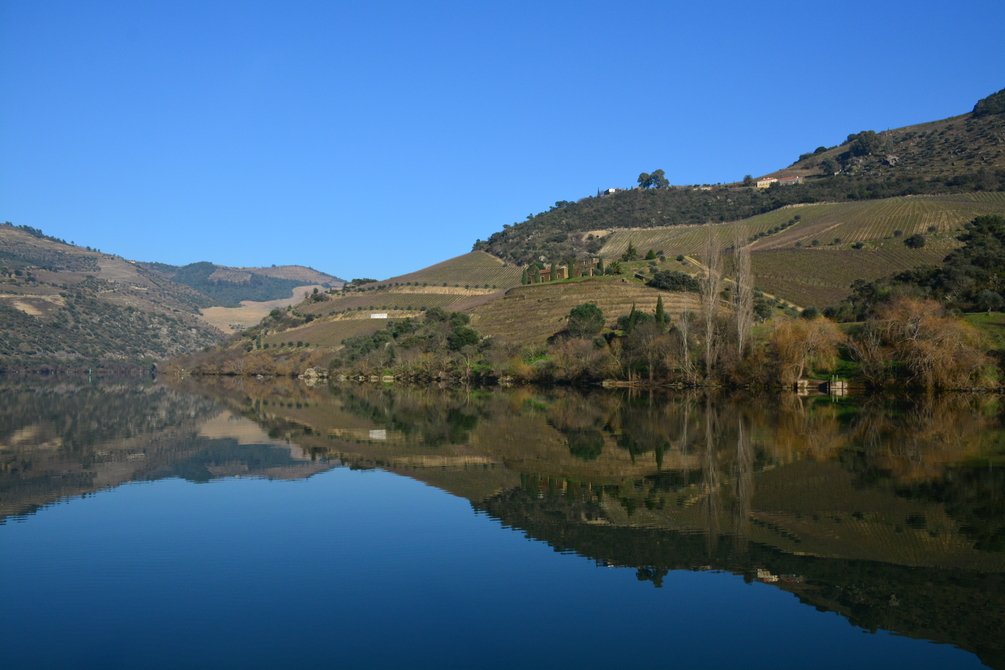
\includegraphics[width=7truecm]{slike/04_Douro.jpeg}
\caption{Odboj na vodni gladini. Pri majhnih vpadnih kotih je odbojnost
majhna, zato vidimo dno korita, pri večjih
vpadnih kotih postane odbojnost tako velika, da vidimo samo še odboj (levo).
Mirna rečna gladina pri velikih vpadnih kotih deluje kot zrcalo (desno).}
\label{fig:04_OdbojFoto}
\end{figure}

Poglejmo še primer transverzalne magnetne polarizacije. Narišemo odvisnost
amplitudne odbojnosti $r$ in amplitudne prepustnosti $t$ od vpadnega kota 
(slika~\ref{fig:04_redtm}\,a). Zaradi začetne izbire smeri odbite jakosti
električnega polja je predznak pri pravokotnem vpadu drugačen kot pri 
polarizaciji TE in je pozitiven, čeprav se faza valovanja obrne. 
Z naraščajočim vpadnim kotom se amplitudna
odbojnost zmanjšuje in doseže vrednost $r=-1$, ko se vpadni kot
približuje $\alpha = 90\si{\degree}$.\index{Polarizacija!{transverzalna magnetna}}\index{Amplitudna odbojnost!{TM}}\index{Amplitudna prepustnost!{TM}}

Vidimo, da pri nekem kotu zavzame  
vrednost $r = 0$. Vpadni kot, pri katerem je odbojnost za TM polarizirano
valovanje enaka nič, imenujemo Brewstrov kot $\alpha_B$ po škotskem 
znanstveniku Siru Davidu Brewstru (1781--1868). Ta pojav ima pomembno in uporabno
posledico, da je celotno TM polarizirano valovanje pri Brewstrovem kotu prepuščeno. 
Ker amplitudna odbojnost pri Brewstrovem kotu zamenja predznak, se pri tem
kotu tudi spremeni faza odbite svetlobe: pri kotih $\alpha < \alpha_B$ se valovanje
odbije z nasprotno fazo, pri kotih $\alpha > \alpha_B$ pa se TM polarizirano
valovanje odbije z isto fazo.\index{Brewstrov kot}\index{Faza pri odboju}
\index{Brewster, Sir David}
\begin{figure}[ht]
\centering
\def\svgwidth{140truemm} 
\input{slike/04_redtm.pdf_tex}
\caption{Odvisnost amplitudne odbojnosti in amplitudne prepustnosti (a) ter odbojnosti in 
prepustnosti (b) za TM polarizirano valovanje v odvisnosti od vpadnega kota $\alpha$. Kot
$\alpha_B$ označuje Brewstrov kot.}
\label{fig:04_redtm}
\end{figure}

Odbojnost in prepustnost TM polariziranega valovanja sta prikazani na\index{Odbojnost}\index{Prepustnost}
sliki~\ref{fig:04_redtm}\,b. Odbojnost od začetne vrednosti pri $\alpha=0$
pojema z naraščajočim vpadnim kotom do vrednosti 0, ki jo doseže pri 
Brewstrovem vpadnem kotu $\alpha_B$. Nato odbojnost strmo naraste z naraščajočim vpadnim
kotom do vrednosti 1. Pri velikih vpadnih kotih je zato
gladka meja z optično gostejšo snovjo videti kot zrcalo. Prepustnost preprosto izračunamo 
kot $\mathcal{T} = 1- \mathcal{R}$.

\subsection*{Brewstrov kot}\index{Brewstrov kot}
Brewstrov kot smo vpeljali kot vpadni kot, pri katerem je odbojnost
TM polariziranega valovanja enaka nič. Poglejmo, pri katerem
vpadnem kotu se to zgodi. Amplitudna odbojnost $r$ je po enačbi~(\ref{eq:04_40})
enaka:
\begin{equation}
r = \frac{\tan(\alpha-\beta)}{\tan(\alpha+\beta)}.
\label{eq:04_50}
\end{equation}
Pri vrednosti $\alpha + \beta = \pi/2$ imenovalec v izrazu za $r$ 
naraste v neskončnost. Ker je števec vedno različen od nič -- saj
sta po lomnem zakonu vpadni in lomni kot vedno različna -- je pri 
vrednosti $\alpha + \beta = \pi/2$ odbojnost enaka nič.
Izračunamo $\sin \beta = \sin (\pi/2-\alpha) = \cos \alpha$. 
Iz lomnega zakona (enačba~\ref{eq:04_18}) sledi:
\begin{equation}
n_1 \sin \alpha= n_2 \sin \beta= n_2 \cos \alpha.
\label{eq:04_51}
\end{equation}
Za Brewstrov kot tako velja:
\boxeq{eq:Brewstrovkot}{
\tan \alpha_B = \frac{n_2}{n_1}.
}
Pri prehodu iz zraka v steklo je $\alpha_B = 56\si{\degree}$ in na prehodu
iz zraka v vodo $\alpha_B = 53\si{\degree}$. 

Še enkrat povzemimo pomen Brewstrovega kota: odbojnost za TM polarizirano
valovanje je enaka nič, prepustnost za TM polarizirano valovanje pa enaka 1. Če 
torej TM polarizirana svetloba vpada na mejo pod Brewstrovim kotom, je vsa svetloba
prepuščena. Kadar pa o\-svet\-lju\-je\-mo mejno ploskev z nepolarizirano svetlobo, se 
pri kotu $\alpha_B$ od mejne ploskve odbije samo TE polarizirano
valovanje, TM pa je v celoti prepuščeno. Na ta preprost način
iz nepolarizirane svetlobe dobimo linearno polarizirano valovanje.
\vglue-5truemm
\begin{remark}
Pri Brewstrovem kotu je odbojnost TM polariziranega valovanja točno 
enaka nič, vendar je tudi pri kotih, ki so blizu $\alpha_B$, 
odbojnost precej manjša kot za TE polarizirano valovanje. 
To s pridom uporabljamo pri polarizacijskih sončnih očalih ali fotografskih
filtrih. Ker se od površine, na primer vodne gladine, zasnežene pokrajine
ali gladke ceste, odbije razmeroma malo TM polariziranega valovanja, 
je odbita svetloba pretežno TE linearno polarizirana. Če sončna
očala ali fotografski filter delujejo kot polarizator, ki TE polarizirane 
svetlobe ne prepušča, bistveno zmanjšamo količino odbite svetlobe in 
``bleščanje'' površine. Sončna očala so linearni polarizatorji, večina 
fotografskih polarizacijskih filtrov pa vstopno linearno polarizacijo spremeni
v cirkularno, saj bi linearno polarizirana svetloba lahko motila delovanje svetlomera.\index{Polarizacijski filter}
\begin{figure}[htp]
\centering
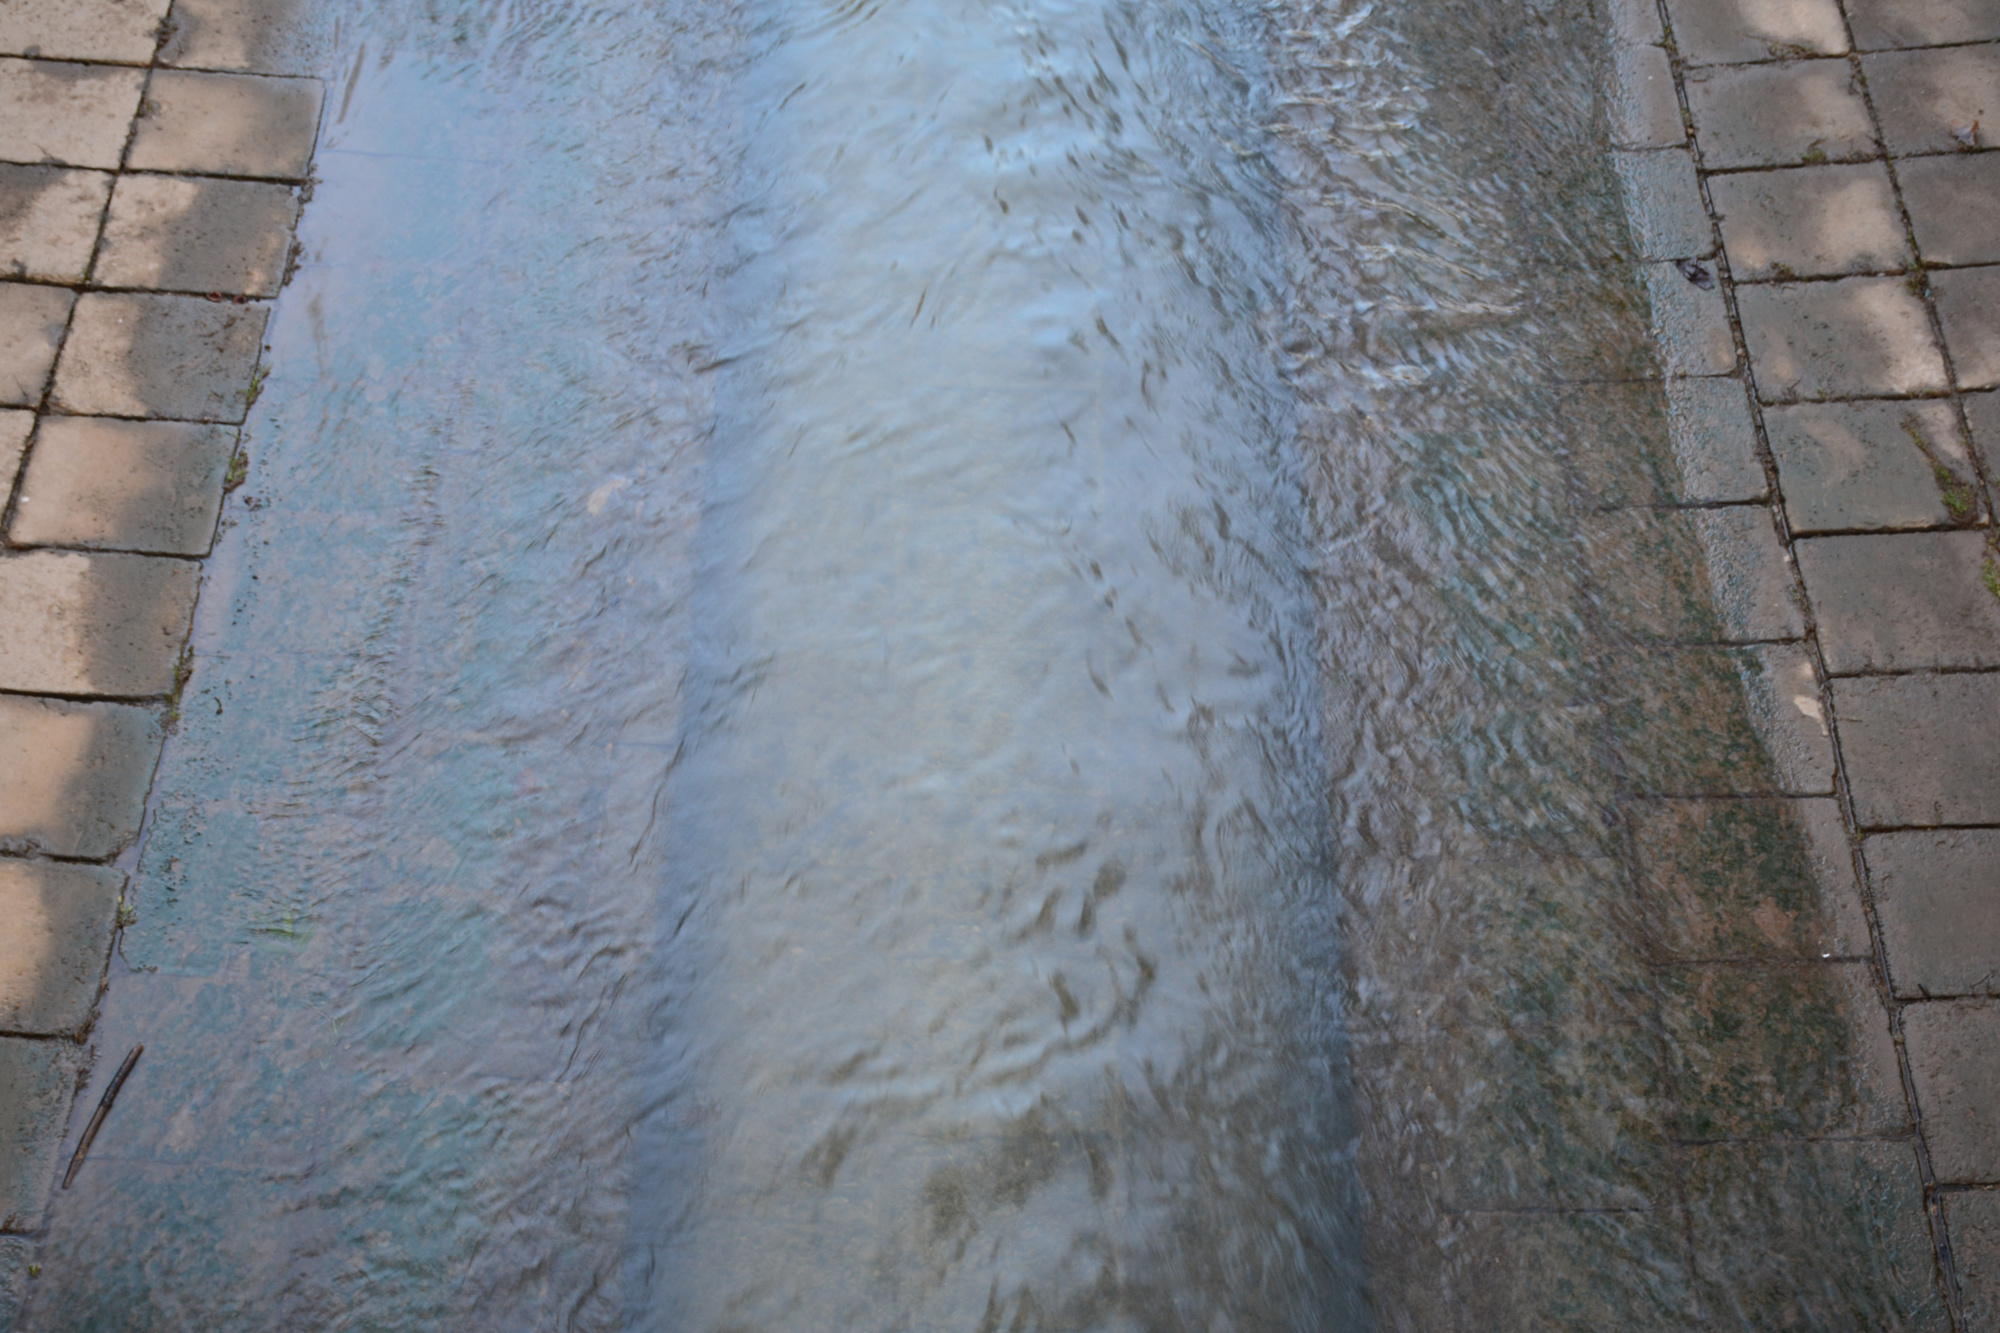
\includegraphics[width=7truecm]{slike/04_photos_voda1.jpg}\hfill
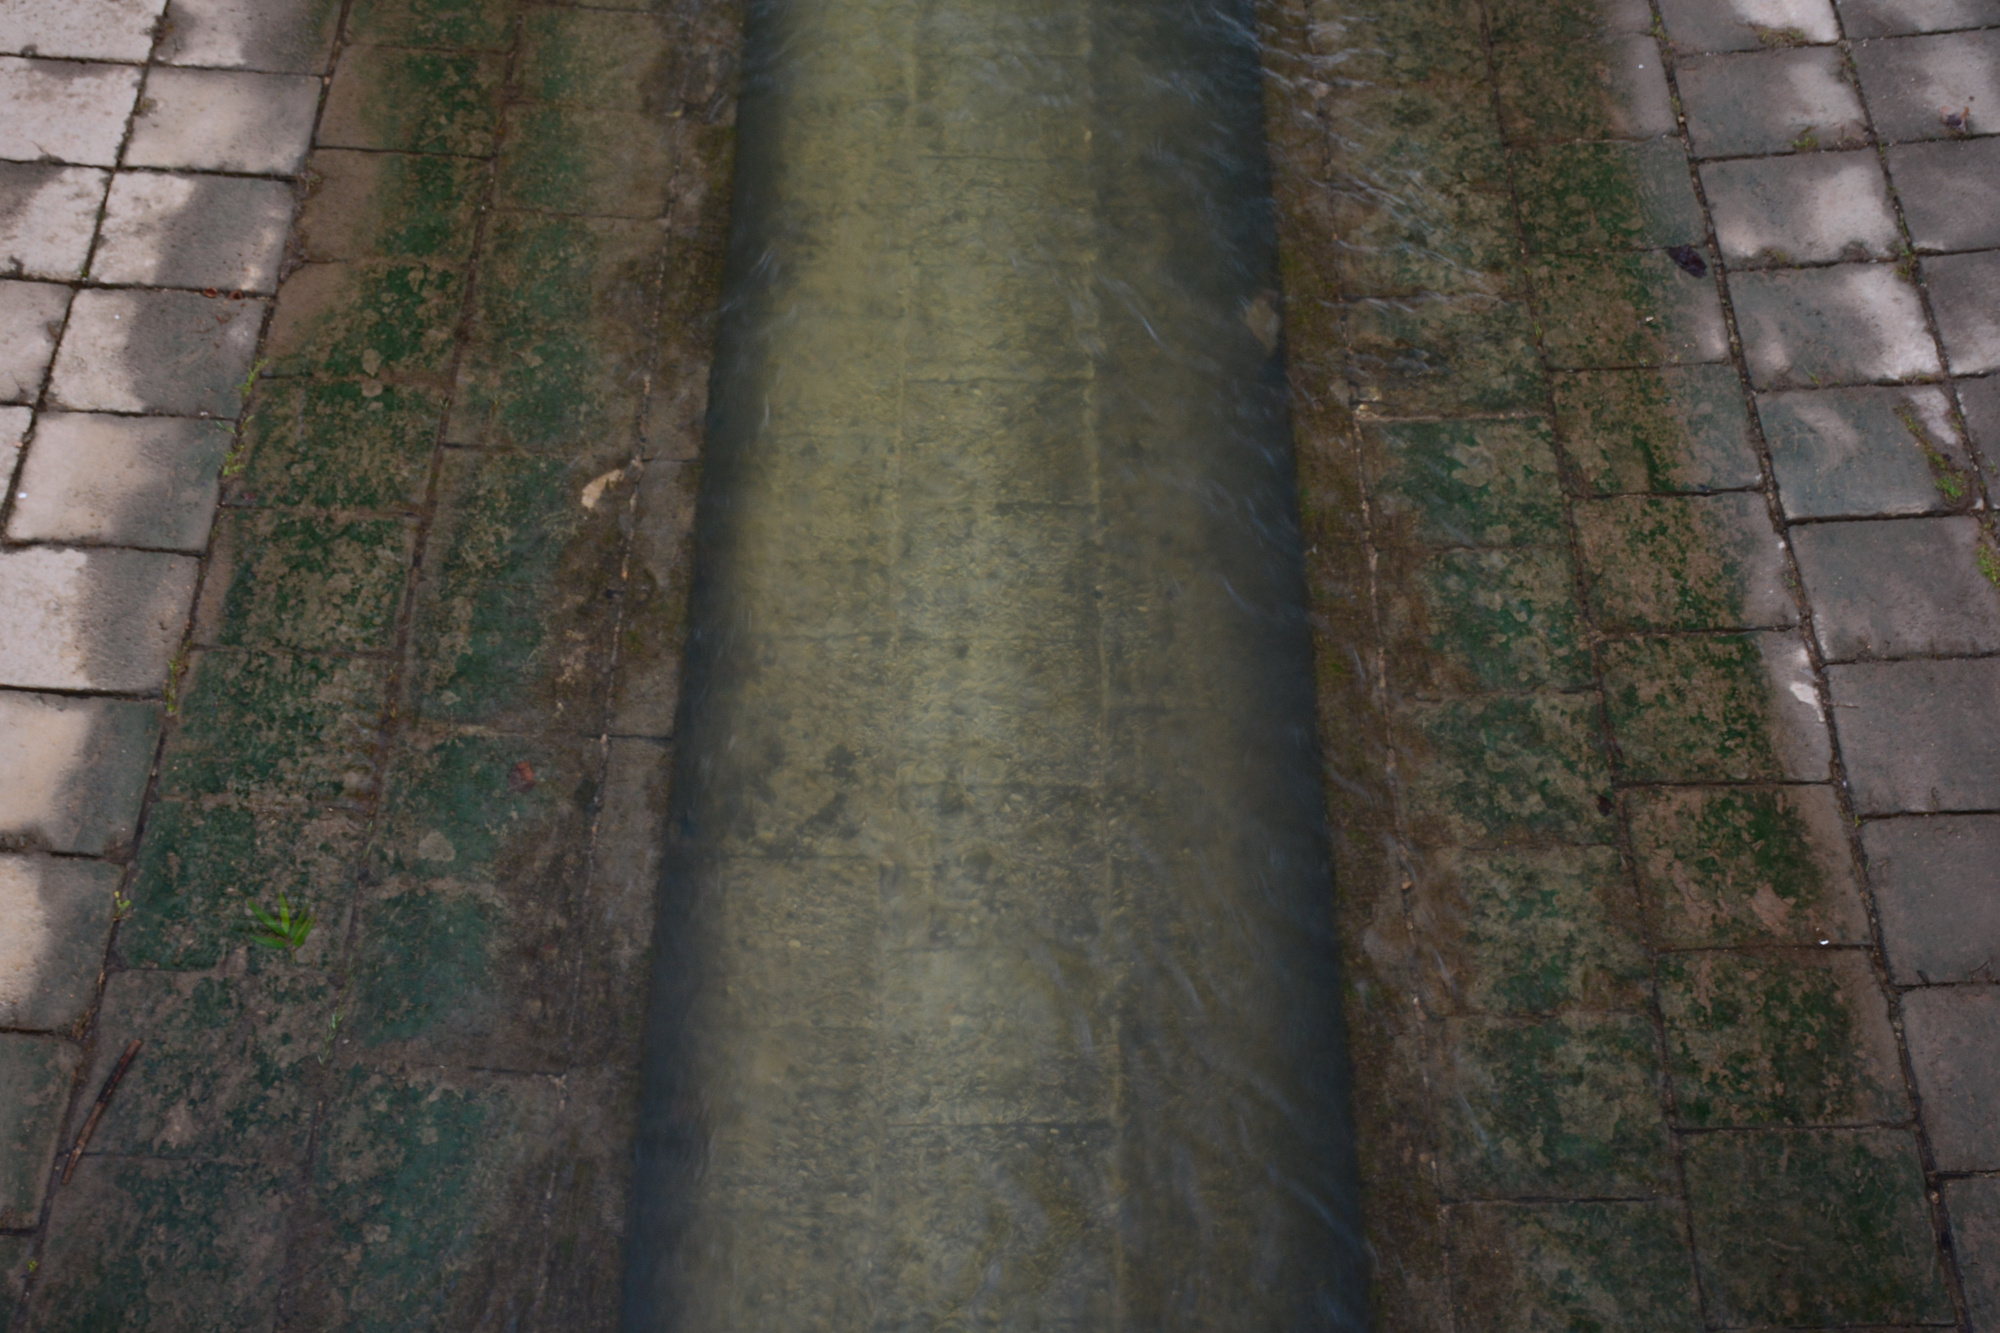
\includegraphics[width=7truecm]{slike/04_photos_voda2.jpg}
\caption{Odsev na vodni gladini preprečuje, da bi videli v globino vode (levo).
Ker je odbita svetloba pretežno linearno polarizirana, jo s polarizacijskim 
filtrom odstranimo in tako vidimo dno potoka (desno).}
\label{fig:04_odsevvoda}
\end{figure}

\begin{figure}[htp]
\centering
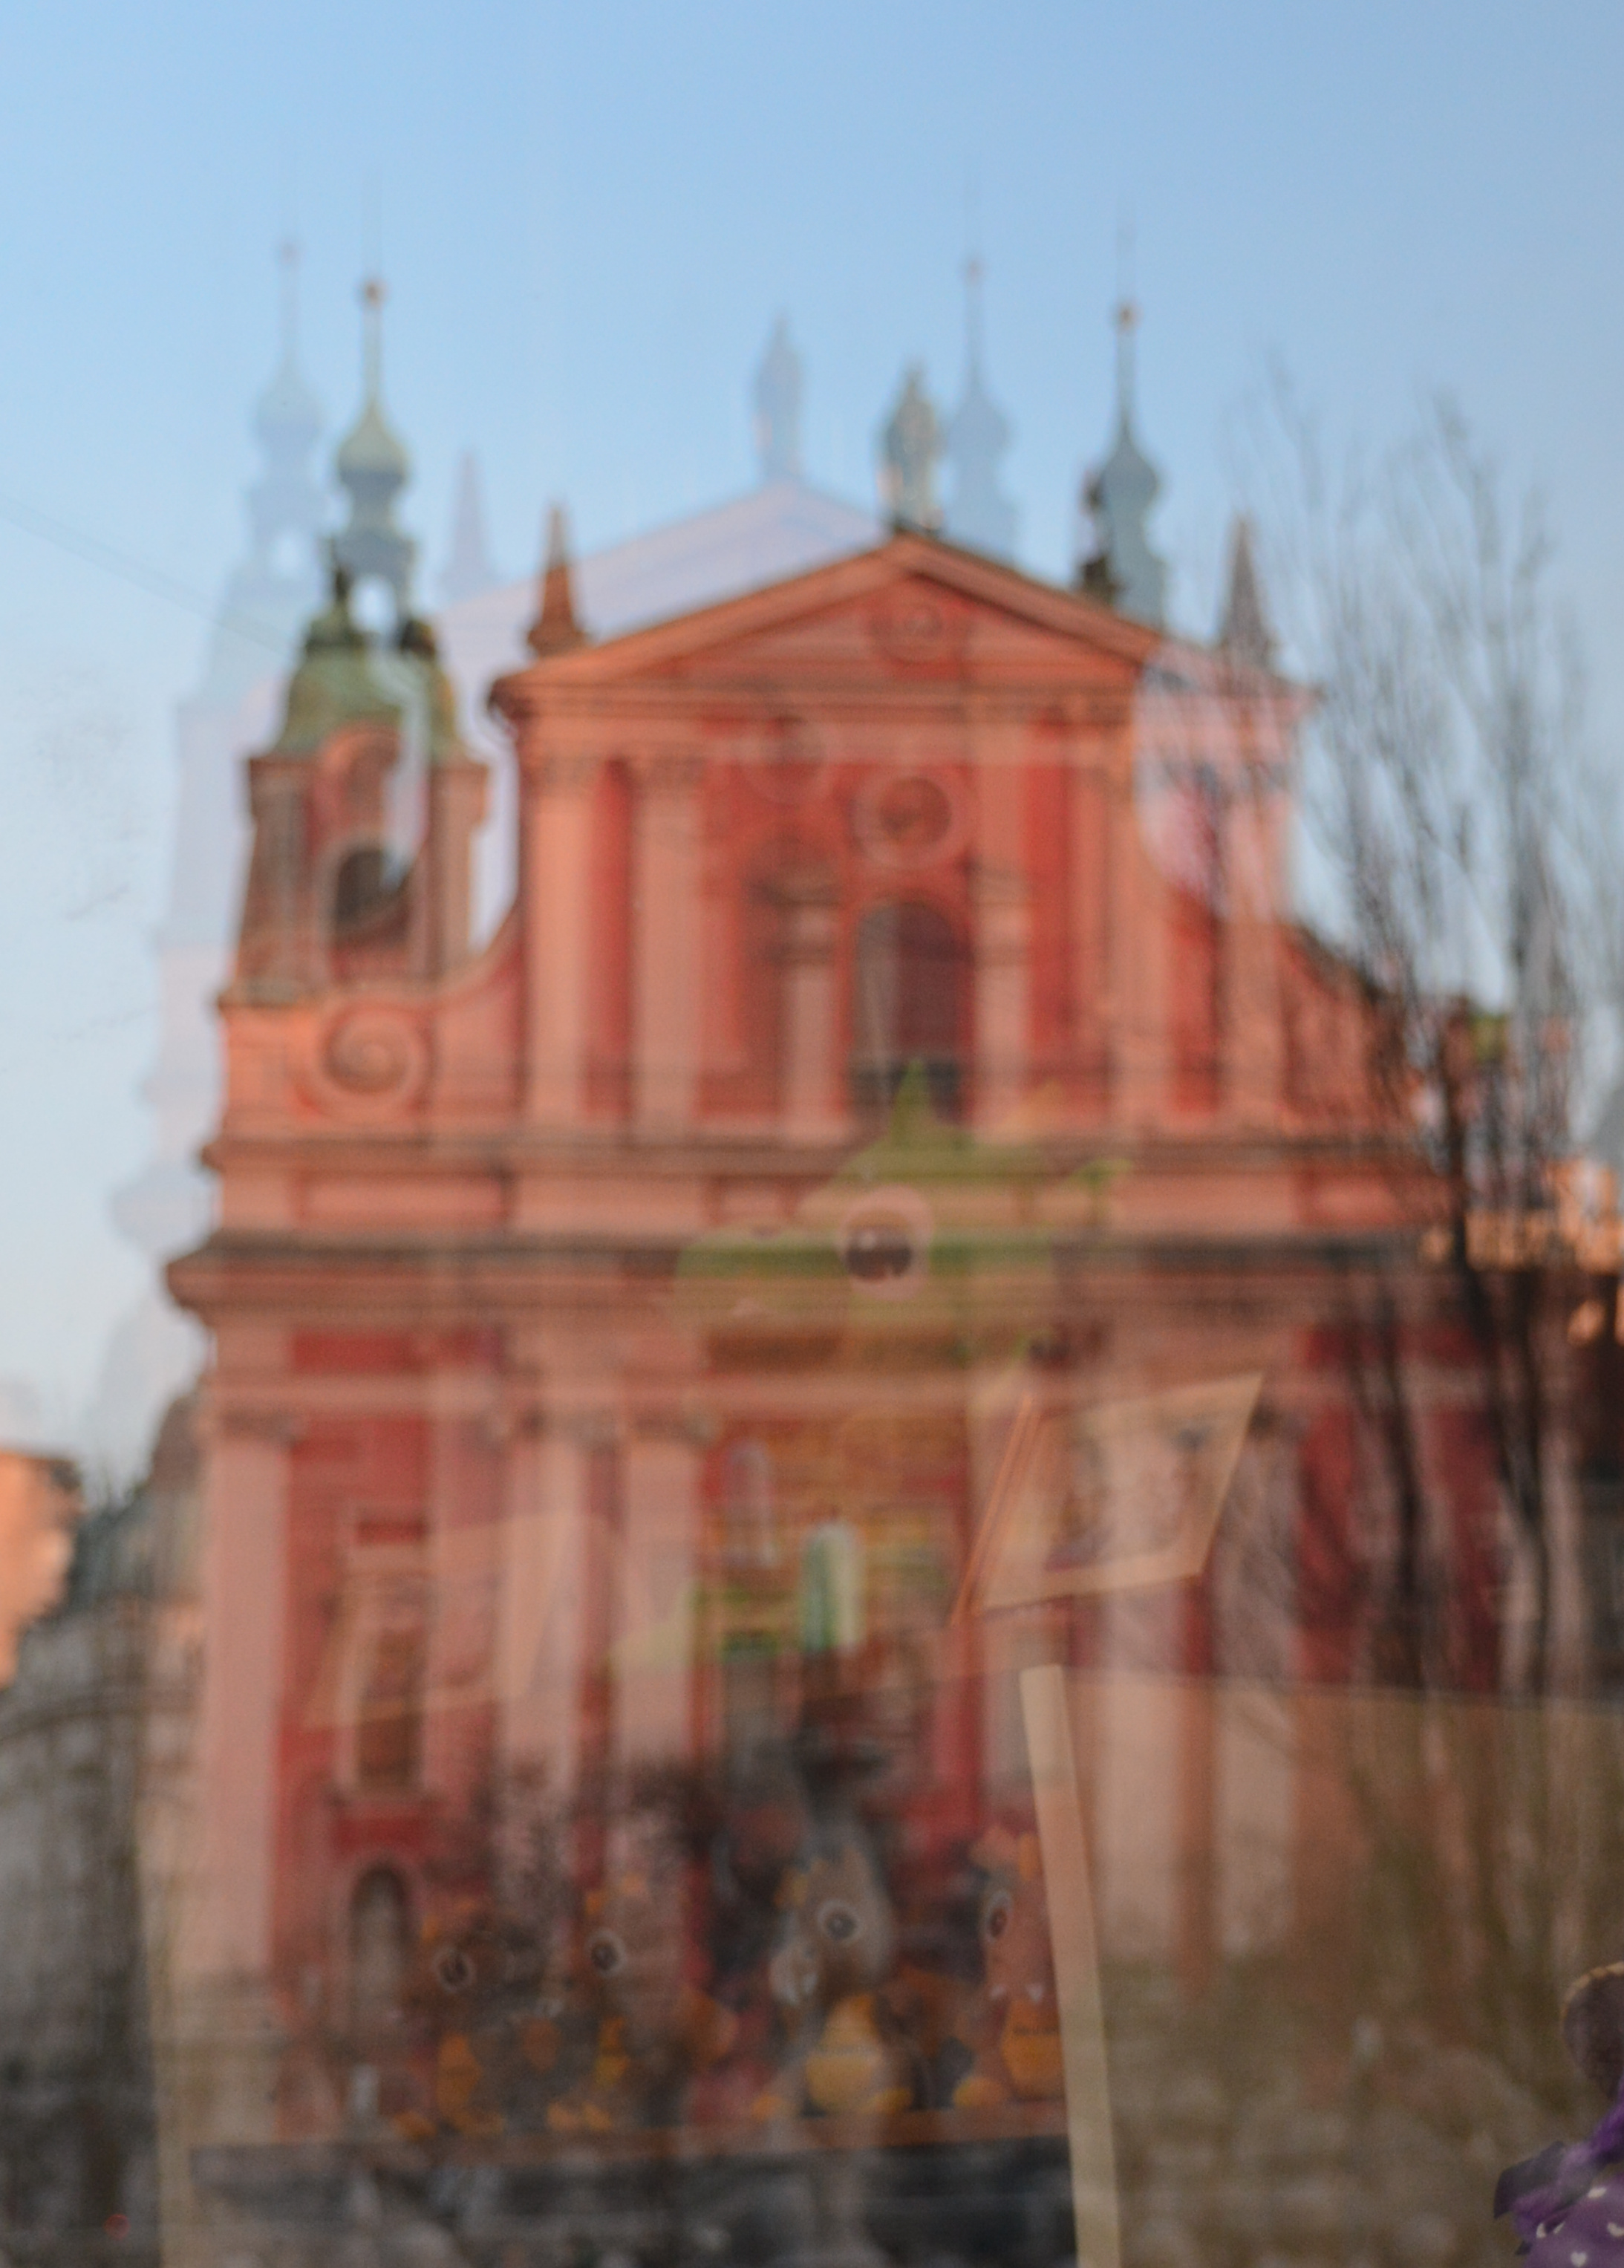
\includegraphics[width=6truecm]{slike/04_photos_zmaj2.jpg}\qquad \qquad
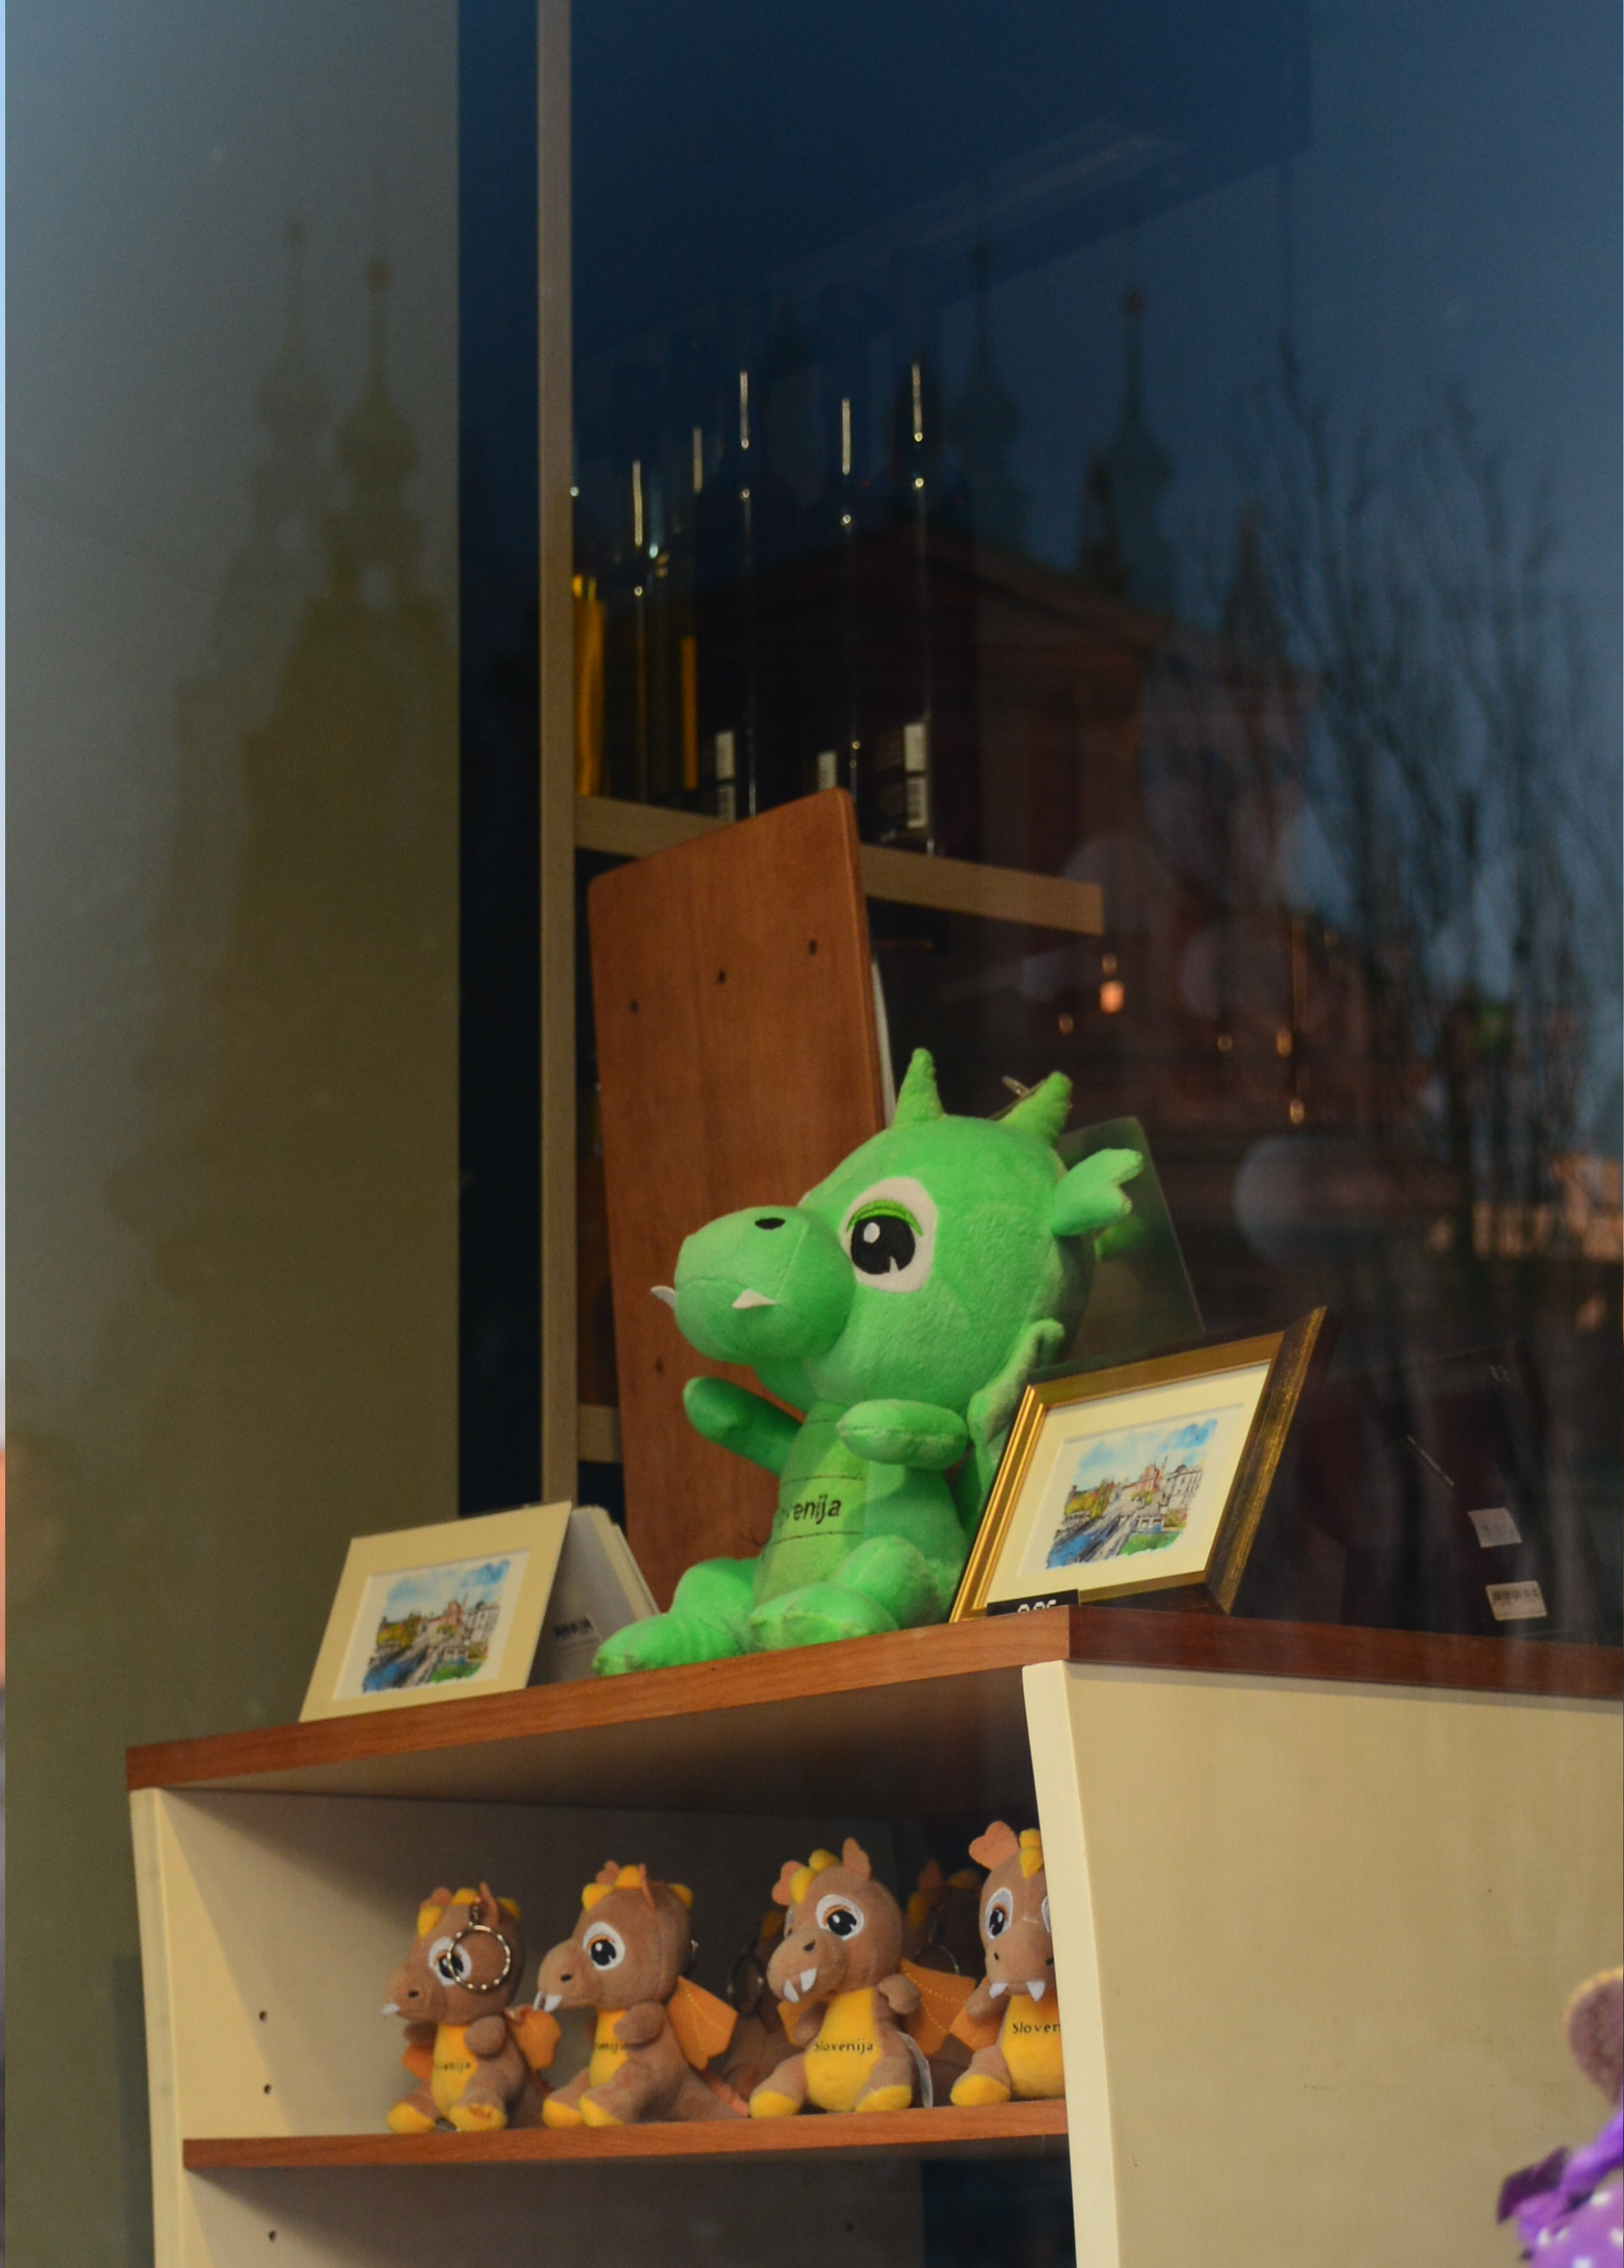
\includegraphics[width=6truecm]{slike/04_photos_zmaj1.jpg}
\caption{Odsev v izložbenem oknu (levo) in isti motiv, slikan s polarizacijskim 
filtrom (desno), ki omogoča pogled v izložbo.}
\label{fig:04_odsevzmaj}
\end{figure}
\begin{figure}[!htp]
\centering
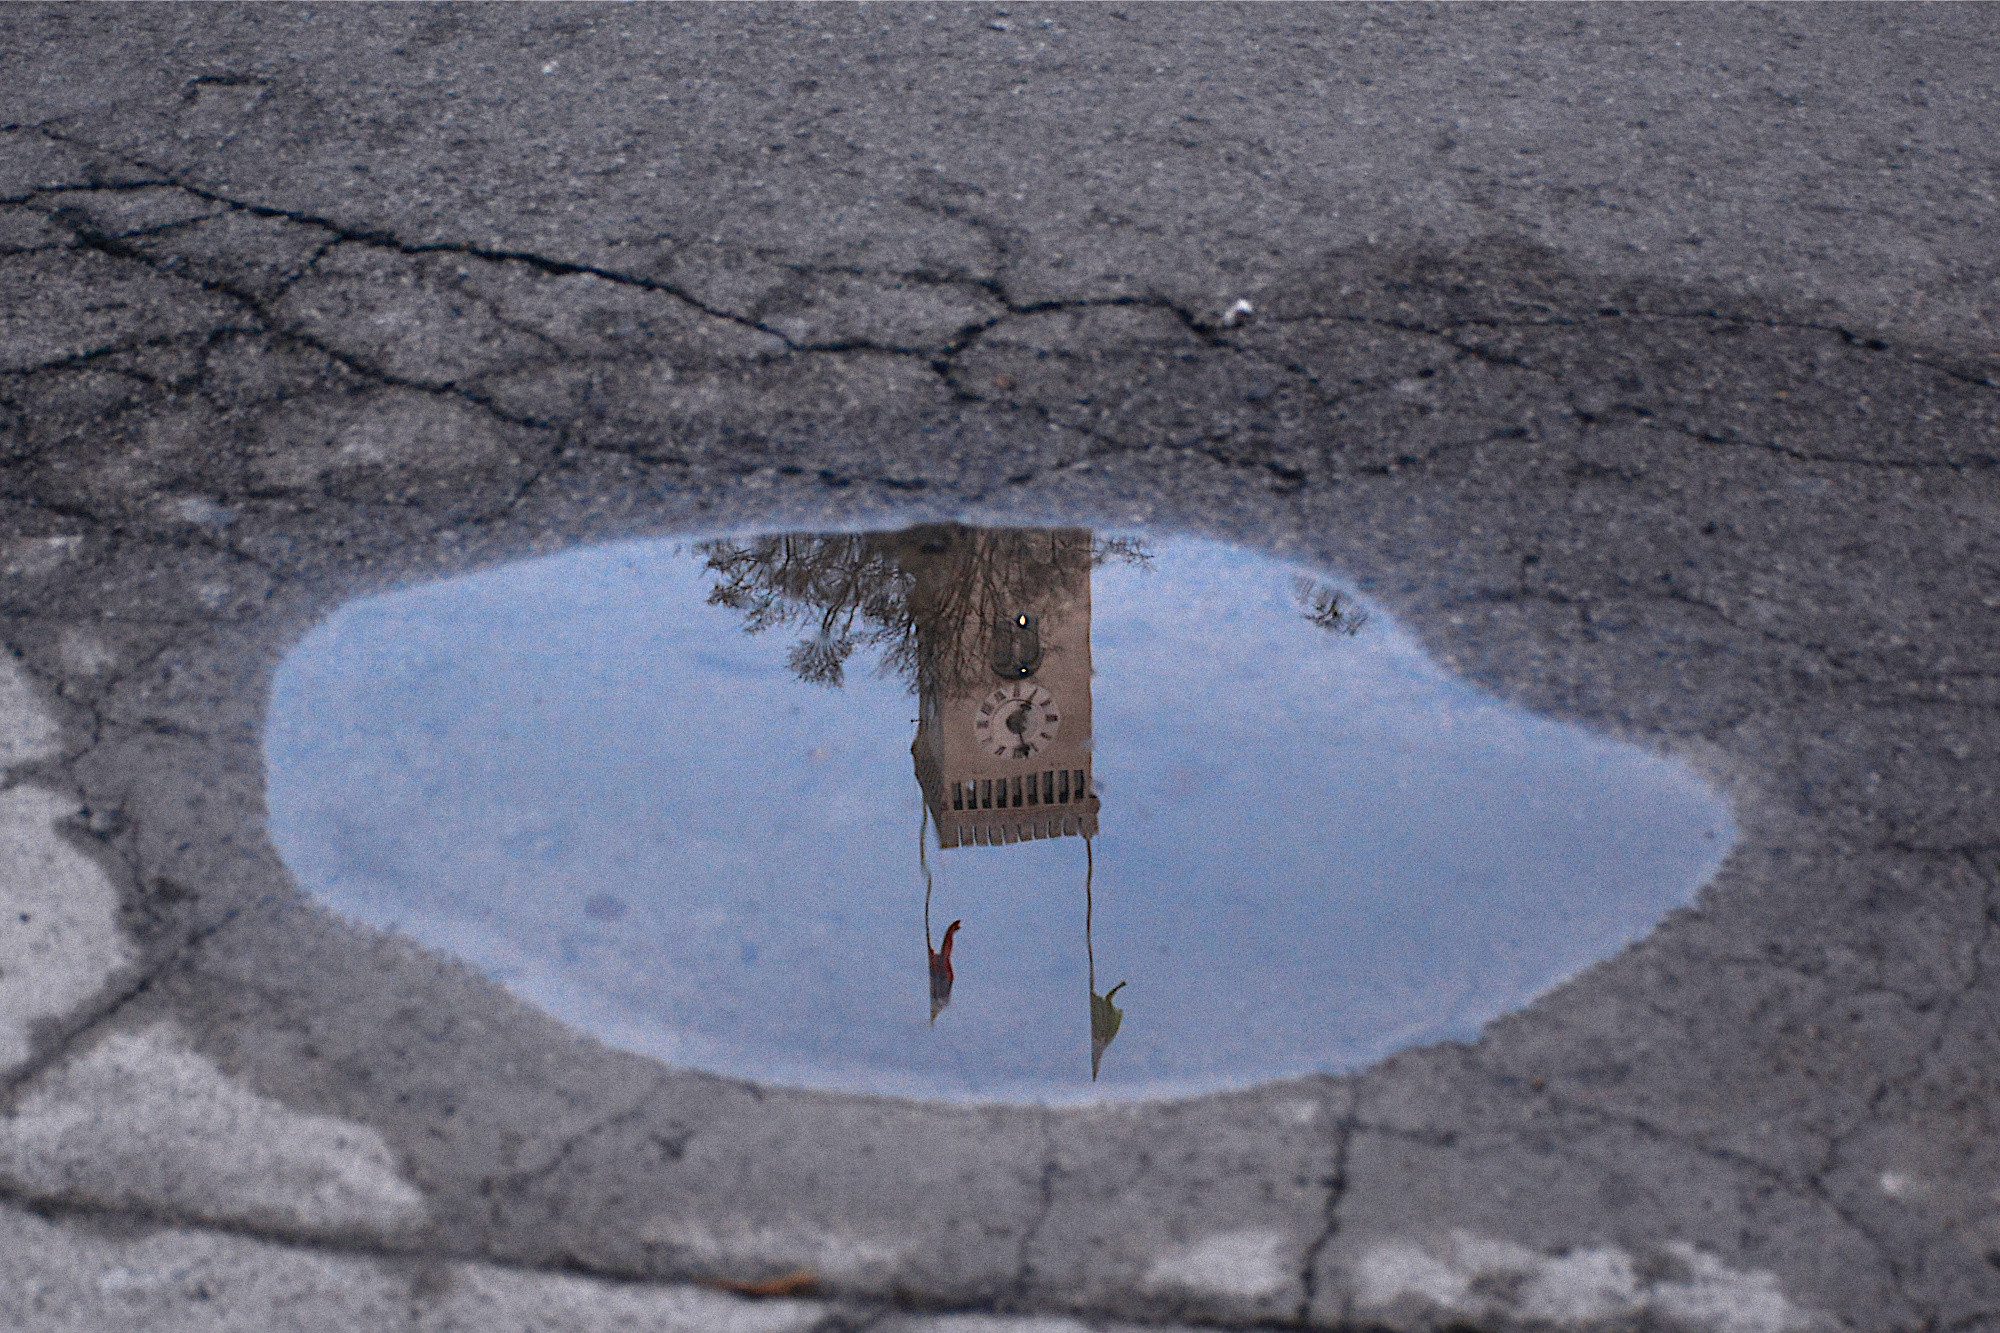
\includegraphics[width=7truecm]{slike/04_photos_grad1.jpg}\hfill
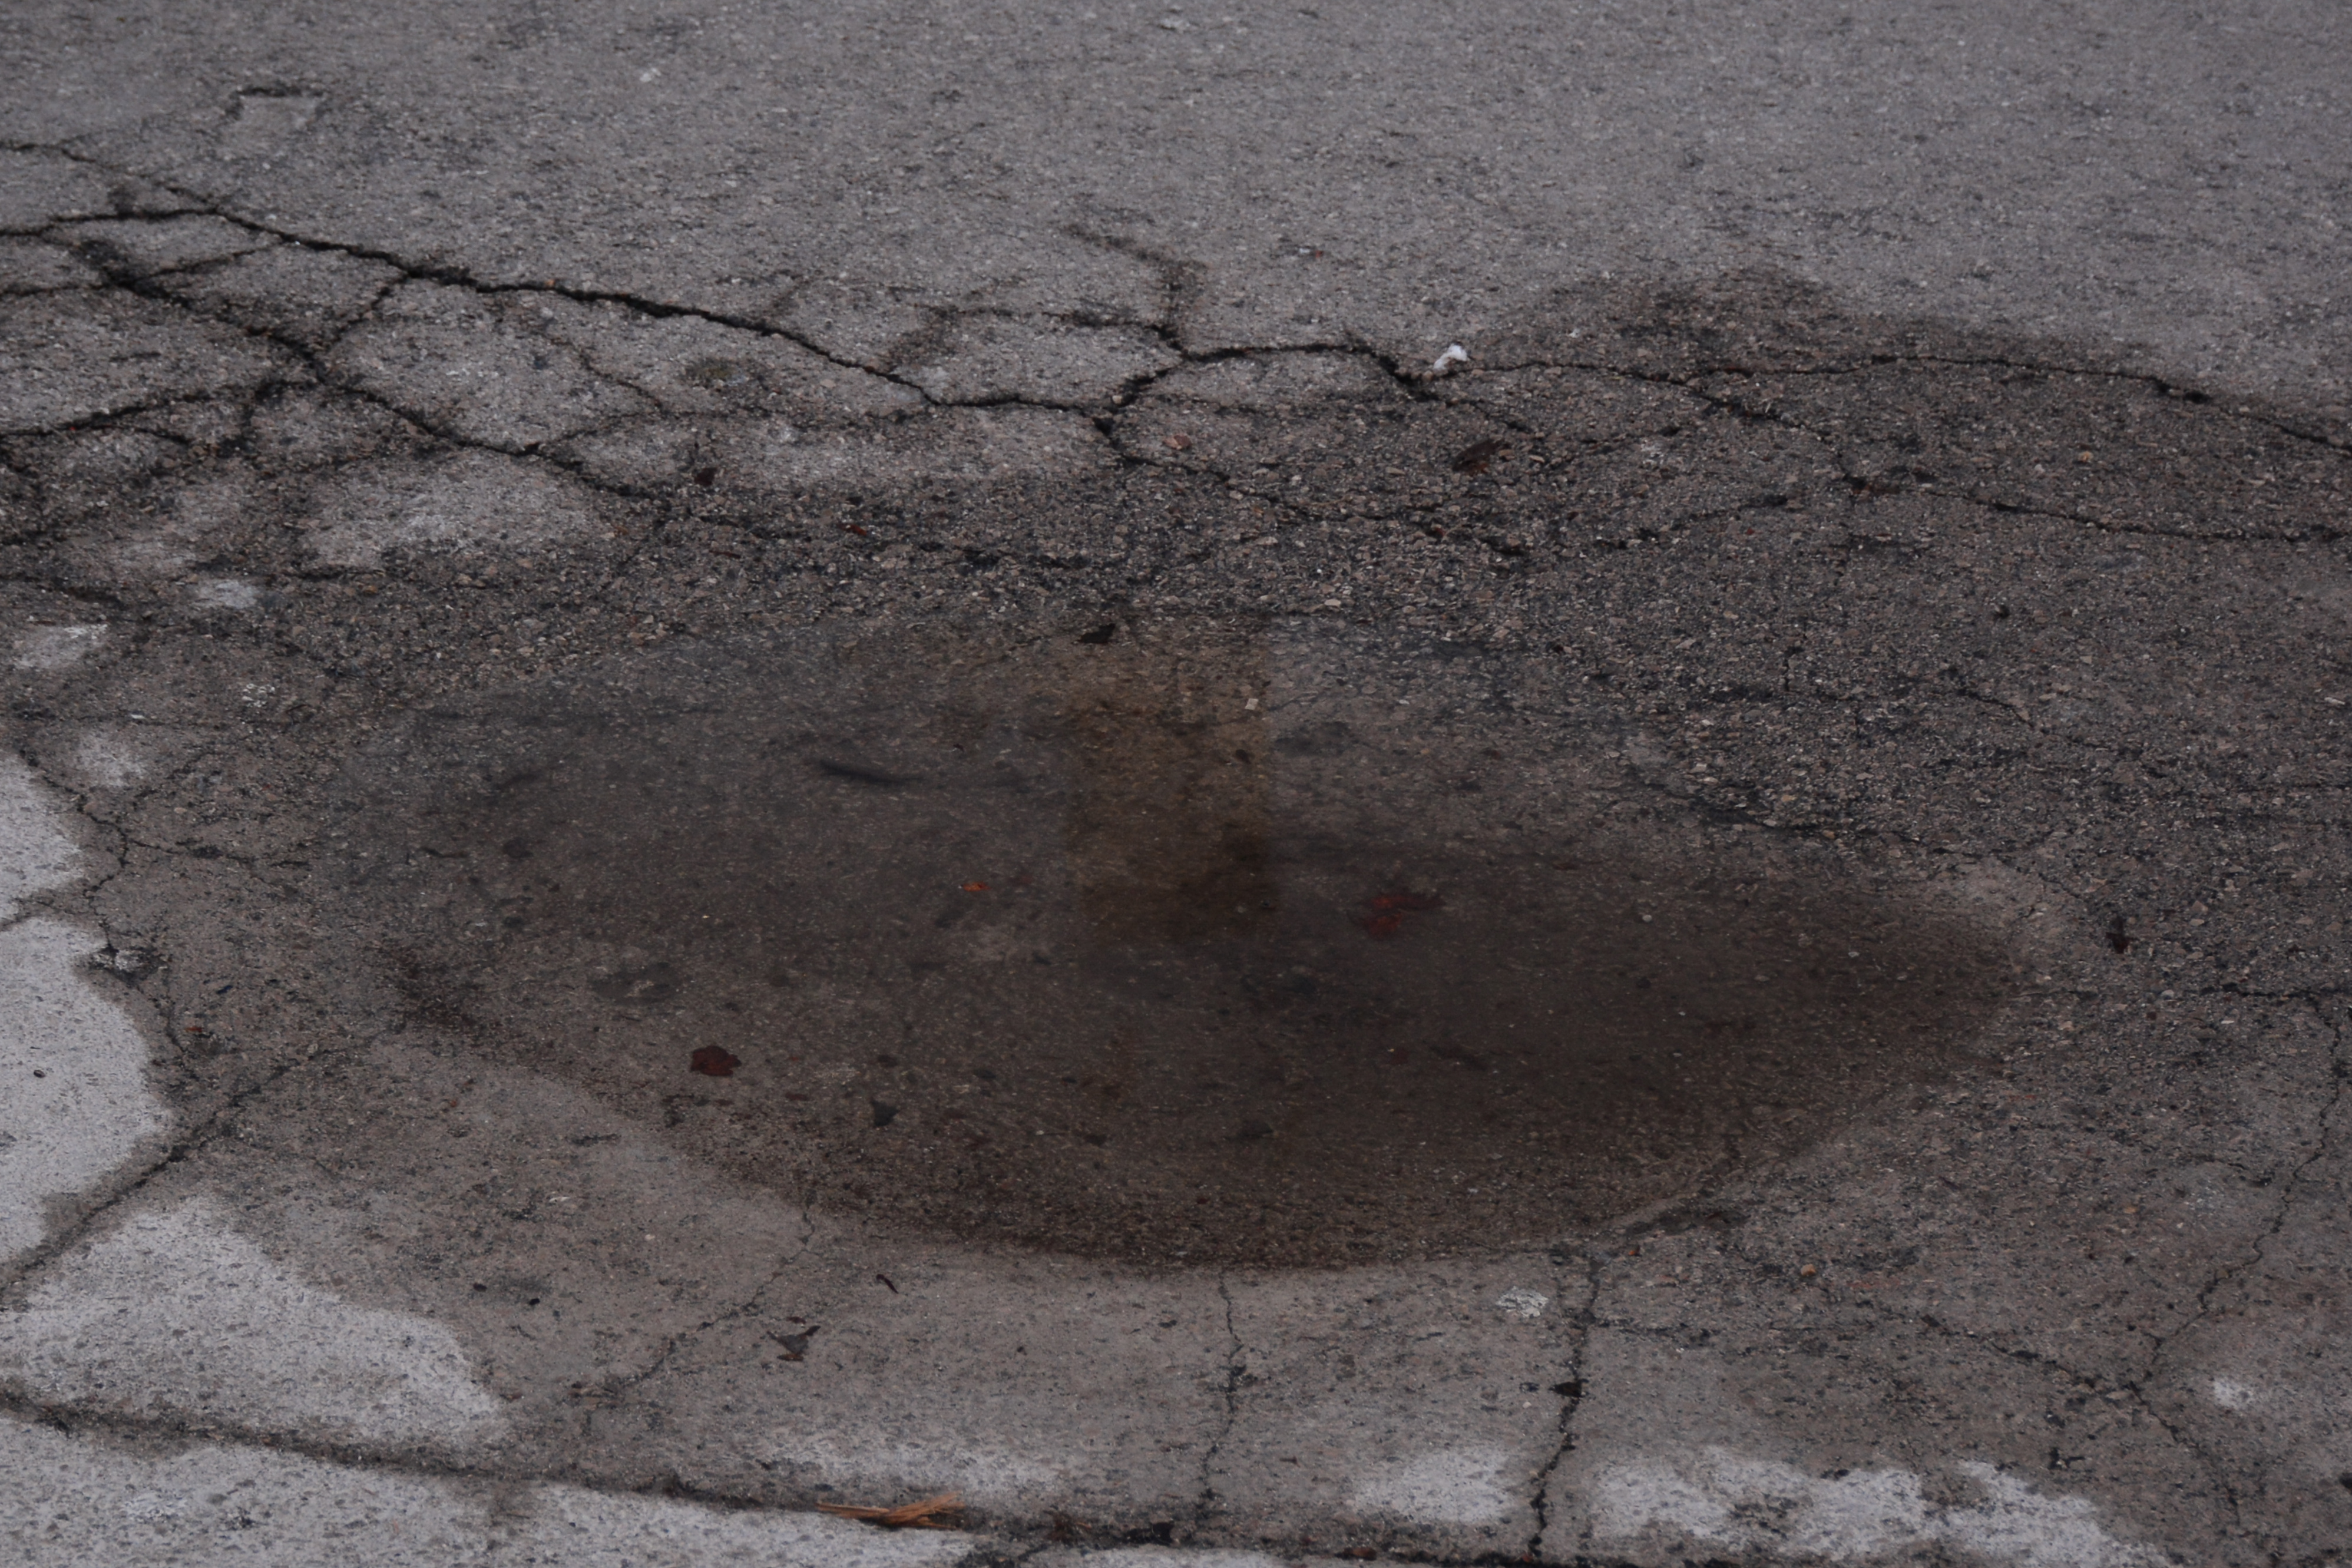
\includegraphics[width=7truecm]{slike/04_photos_grad2.jpg}
\caption{Odsev v luži (levo) in isti motiv, slikan s polarizacijskim filtrom (desno). 
Polarizirano odbito svetlobo zaustavi fotografski filter, zato odsev ni več viden,
vidno pa je dno luže.}
\label{fig:04_odsevgrad}
\end{figure}
\begin{figure}[!htp]
\centering
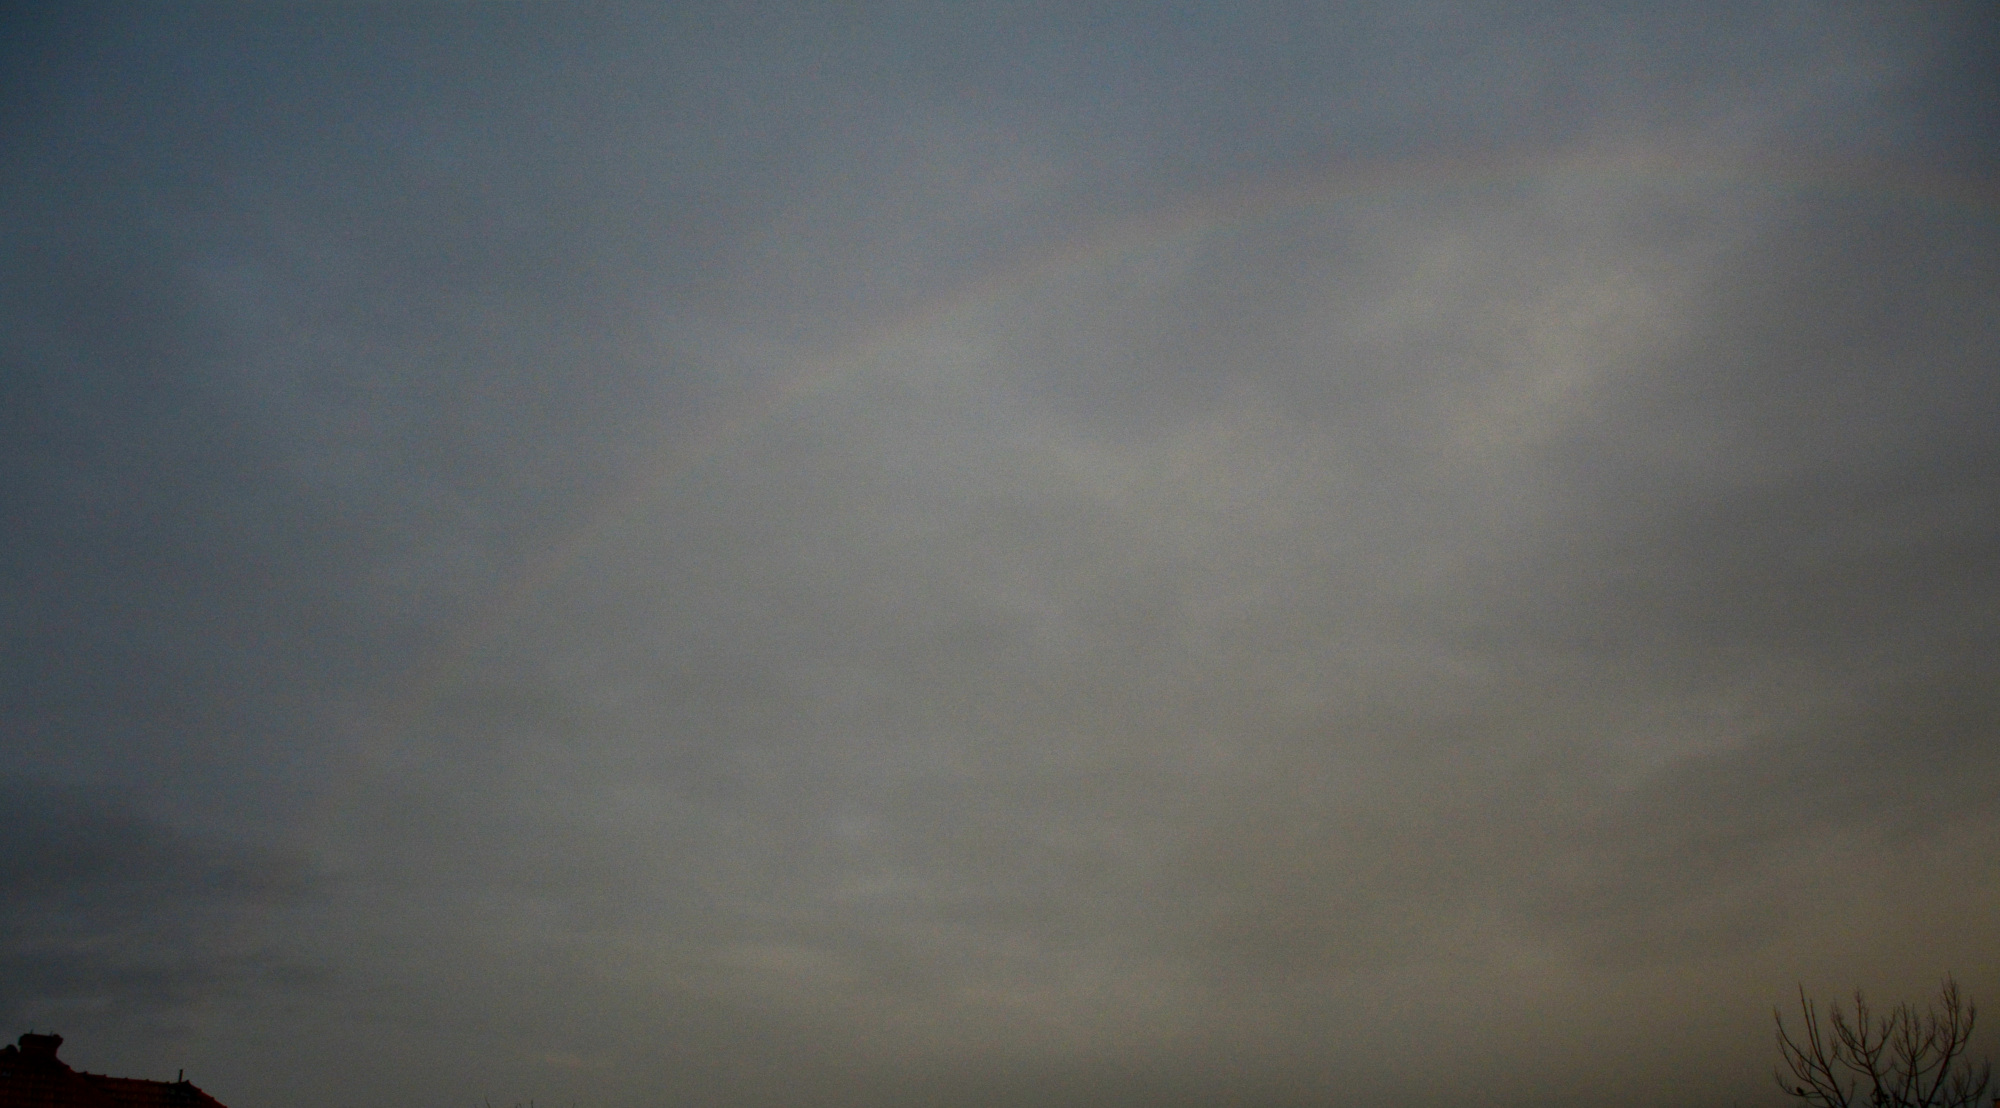
\includegraphics[width=7truecm]{slike/04_PolMavrica_a.jpg}\hfill
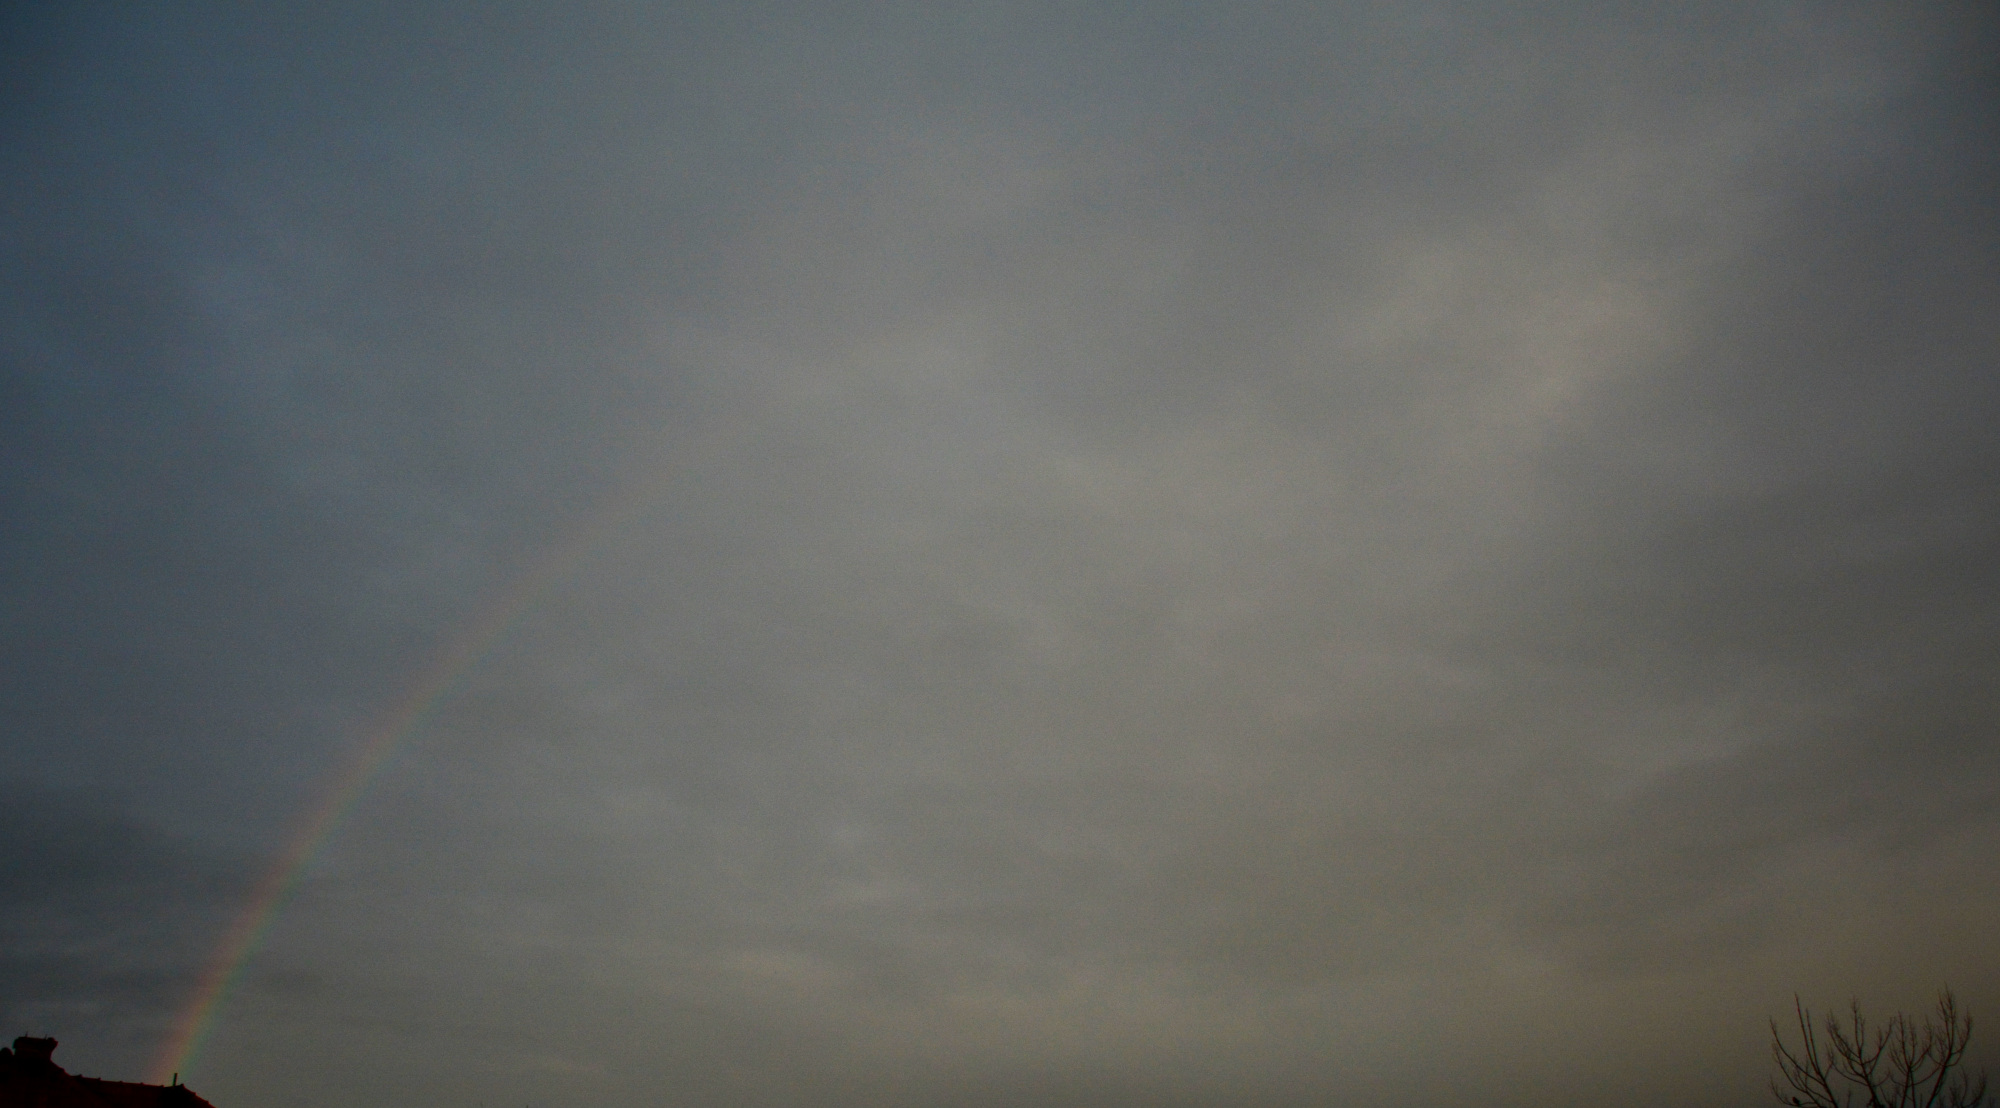
\includegraphics[width=7truecm]{slike/04_PolMavrica_b.jpg}
\caption{Mavrica nastane z odbojem svetlobe v dežnih kapljicah (glej poglavje~\ref{chap:disperzija}).
Ker je odbojni kot blizu Brewsterjevega kota, je mavrica pretežno polarizirana, kar pokažemo z linearnim 
polarizatorjem (smer polarizatorja označuje puščica). Šibko vidni zgornji lok mavrice na desni sliki povsem 
izgine, osnovni mavrični lok pa je viden le še ob robovih.}\index{Mavrica}
\label{fig:04_MavricaFoto}
\end{figure}
\end{remark}

\section{Prehod v optično redkejšo snov in totalni odboj}\index{Lom!{v optično redkejšo snov}}
Pri prehodu v snov z manjšim lomnim količnikom pride do novih zanimivih pojavov.
Primer tega je prehod svetlobe iz vode ali stekla v zrak, ko je $n_1>n_2$.
Izhajamo iz lomnega zakona (enačba~\ref{eq:04_18}) in zapišemo lomni kot:\index{Lomni kot}
\begin{equation}
\beta = \arcsin \left(\frac{n_1}{n_2}\sin \alpha\right)\!\!.
\label{eq:04_52}
\end{equation}
Pri določeni vrednosti vpadnega kota $\alpha_m$ 
argument doseže vrednost $1$ in lomni kot
postane enak $\beta = 90\si{\degree}$. Za vpadne kote, ki so večji od 
mejnega in za katere velja
$\alpha> \alpha_m$, enačba nima več rešitve. Takrat govorimo o totalnem 
ali popolnem odboju (slika~\ref{fig:04_totalni}\,a). Mejni kot 
totalnega odboja izračunamo kot:\index{Totalni odboj}\index{Mejni kot totalnega odboja}
\boxeq{eq:totalni}{
\alpha_m = \arcsin\left(\frac{n_2}{n_1}\right)\!\!.
}
V steklu z lomnim količnikom $n_1=1,5$ je mejni kot totalnega odboja
enak $\alpha_m = 41,8\si{\degree}$, v vodi z lomnim količnikom 
$n_1 = 1,33$ pa $\alpha_m = 48,7\si{\degree}$.
\begin{figure}[ht]
\centering
\def\svgwidth{140truemm} 
\input{slike/04_totalni.pdf_tex}
\caption{Svetloba vpada iz snovi z večjim lomnim količnikom v snov z manjšim lomnim količnikom.
Pri vpadnih kotih, ki so večji od mejnega kota totalnega odboja $\alpha_m$, se svetloba totalno odbije (a). Pri računu
si pomagamo s sliko loma (b).}
\label{fig:04_totalni}
\end{figure}

Izračunajmo odbojnost in prepustnost najprej za TE polarizacijo.\index{Amplitudna odbojnost!{TE}}\index{Amplitudna prepustnost!{TE}}\index{Polarizacija!{transverzalna električna}}
Po enačbi~(\ref{eq:TEr}) je:
\begin{equation}
r = \frac{n_1 \cos \alpha - n_2 \sqrt{1 - (\sin \alpha \cdot n_1/n_2)^2}}
{n_1 \cos \alpha + n_2 \sqrt{1 - (\sin \alpha \cdot n_1/n_2)^2}}.
\label{eq:04_53}
\end{equation}
Za vrednosti vpadnega kota $\alpha > \alpha_m$ je argument korena
negativen, zato postane člen imaginaren. Zapišimo:
\begin{equation}
r = \frac{n_1 \cos \alpha - i n_2 \kappa}{n_1 \cos \alpha + i n_2\kappa},
\label{eq:04_54}
\end{equation}
pri čemer je:
\begin{equation}
\kappa = \sqrt{\left(\frac{n_1}{n_2}\sin \alpha \right)^2-1}  = 
\sqrt{\left(\frac{\sin \alpha}{\sin \alpha_m}\right)^2 -1}.
\label{eq:04_55}
\end{equation}
Potem izračunamo odbojnost $\mathcal{R}$:\index{Odbojnost}
\begin{equation}
\mathcal{R} = |r|^2 = \frac{n_1 \cos \alpha -i n_2\kappa}{n_1 \cos \alpha +i n_2\kappa}
\cdot \frac{n_1 \cos \alpha +i n_2\kappa}{n_1 \cos \alpha -i n_2\kappa} = 1.
\label{eq:04_56}
\end{equation}
Pri vpadnih kotih, ki so večji od mejnega kota totalnega odboja, je $\mathcal{R} = 1$
in vsa vpadna svetloba se odbije. Za smer odbitega žarka velja odbojni zakon. 
\begin{figure}[ht]
\centering
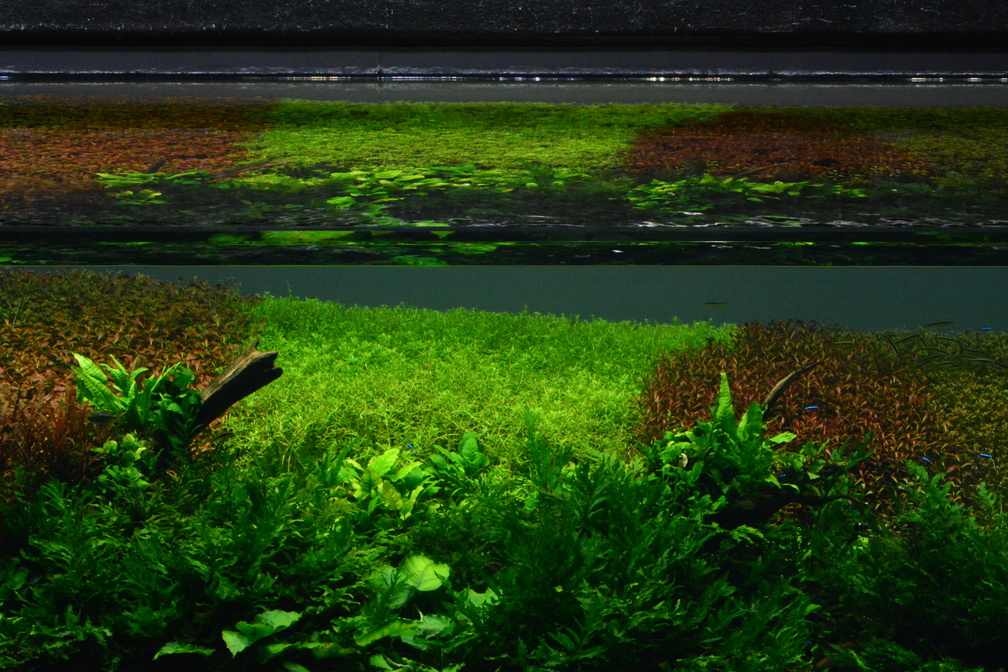
\includegraphics[width=10truecm]{slike/04_TotalniOdbojFoto.jpg}
\caption{Totalni odboj na gladini akvarija}
\vglue-5truemm
\label{fig:04_TotalniFoto}
\end{figure}

Narišimo amplitudno odbojnost in amplitudno prepustnost za TE valovanje 
(slika~\ref{fig:04_goste}\,a). 
Ker je $n_1>n_2$, je amplitudna odbojnost pri pravokotnem vpadu pozitivna. 
Pri pravokotnem vpadu svetlobe na optično redkejšo snov se torej
faza ohranja. Amplitudna odbojnost z naraščajočim vpadnim kotom narašča 
do vrednosti $r=1$, ki jo doseže pri mejnem kotu totalnega odboja. 
Prepustnost, ki jo izračunamo
kot $t = 1+r$, zavzame pri pravokotnem vpadu vrednost nekaj nad 1,
nato pa narašča do vrednosti $t=2$, ki jo doseže pri $\alpha = \alpha_m$. 
To, da je prepustnost večja od 1, nas ne sme motiti, saj gre za
razmerje med amplitudami valovanja in ne med energijskimi tokovi.
\begin{figure}[ht]
\centering
\def\svgwidth{140truemm} 
\input{slike/04_goste.pdf_tex}
\caption{Odvisnost amplitudne odbojnosti in amplitudne prepustnosti (a) ter odbojnosti in 
prepustnosti (b) za TE polarizirano valovanje v odvisnosti od vpadnega kota $\alpha$. 
Pri kotih, ki so večji od mejnega kota $\alpha_m$, se svetloba totalno odbije.}
\label{fig:04_goste}
\end{figure}

Na sliki (slika~\ref{fig:04_goste}\,b) sta prikazani še odbojnost $\mathcal{R}$ 
in prepustnost $\mathcal{T}$. Odbojnost od neke začetne vrednosti homogeno\index{Prepustnost}
narašča do $1$ pri mejnem kotu totalnega odboja. Za vse vpadne kote $\alpha$, ki
so večji od mejnega kota totalnega odboja $\alpha_m$, je odbojnost $\mathcal{R} = 1$ in 
prepustnost $\mathcal{T} = 0$.

Za TM polarizacijo amplitudna odbojnost, ki homogeno\index{Polarizacija!{transverzalna magnetna}}
narašča od začetne negativne vrednosti do 1 pri mejnem\index{Amplitudna odbojnost!{TM}}
kotu totalnega odboja, pri Brewstrovem kotu zavzame vrednost 0 (slika~\ref{fig:04_gostm}\,a). 
Tako sta pri prehodu TM polariziranega valovanja v optično redkejšo
snov pomembna dva kota: Brewstrov kot $\alpha_B$ in mejni kot totalnega odboja $\alpha_m$.
Pri prvem je odbojnost enaka nič, pri drugem pa 1. Amplitudna prepustnost $t$ pri mejnemu kotu 
totalnega odboja doseže vrednost $t>2$,\index{Amplitudna prepustnost!{TM}}
saj v enačbi~(\ref{eq:TMt}) nastopa še razmerje lomnih količnikov, ki je 
večje od 1. 
\begin{figure}[ht]
\centering
\def\svgwidth{140truemm} 
\input{slike/04_gostm.pdf_tex}
\caption{Odvisnost amplitudne odbojnosti in amplitudne prepustnosti (a) ter odbojnosti in 
prepustnosti (b) za TM polarizirano valovanje v odvisnosti od vpadnega kota $\alpha$. 
Pri kotih, ki so večji od mejnega kota $\alpha_m$, se svetloba totalno odbije. Kot $\alpha_m$
označuje Brewstrov kot.}
\label{fig:04_gostm}
\end{figure}

Odbojnost in prepustnost sta prikazani na sliki~\ref{fig:04_gostm}\,b. Po pričakovanju 
odbojnost z naraščajočim kotom pojema do vrednosti 0, ki jo zavzame pri Brewstrovem kotu, 
nato pa strmo naraste do vrednosti 1, ki jo doseže pri mejnem kotu totalnega odboja. Pri večjih
kotih je odbojnost enaka 1. Prepustnost je največja pri Brewstrovem kotu, nato pa strmo
pade do vrednosti 0 pri totalnem odboju.\index{Odbojnost}\index{Prepustnost}

\begin{remark}
Če z žarkom svetlobe posvetimo v tanko plast z lomnim količnikom večjim od 
lomnega količnika okolice, lahko svetlobo ``ujamemo''. Zaradi
zaporednih totalnih odbojev namreč svetlobni žarek ostaja ujet v tanki plasti in se 
širi praktično brez izgub (slika~\ref{fig:04_vlakno}). Tako lahko na 
preprost način razložimo delovanje optičnih vlaken,\index{Optično vlakno}
po katerih svetloba potuje na zelo dolge razdalje. Optična vlakna so nepogrešljiva
pri modernih telekomunikacijah.
\begin{figure}[ht]
\centering
\def\svgwidth{130truemm} 
\input{slike/04_vlakno.pdf_tex}
\caption{Shema optičnega vlakna z lomnim količnikom $n_1$, ki je večji od lomnega količnika
okolice. Pri dovolj velikih vpadnih kotih se žarek svetlobe na stenah totalno odbije in svetloba
praktično brez izgub potuje po vlaknu.}
\label{fig:04_vlakno}
\end{figure}

\begin{figure}[ht]
\centering
\includegraphics[width=13truecm]{slike/04_vlakno_model.jpg}
\caption{V akrilni valj se svetlobi žarek ujame s totalnim odbojem podobno kot se žarek
ujame v optično vlakno.}
\label{fig:04_vlaknomodel}
\end{figure}
\end{remark}

\begin{remark}
Lomni količnik diamanta je razmeroma velik (okoli 2,4), zato je mejni kot\index{Diamant}
totalnega odboja razmeroma majhen ($\alpha_m \approx 25\si{\degree}$). Diamanti so praviloma
obrušeni tako, da se vpadna svetloba na spodnjih ploskvah totalno odbije, kar da diamantom značilen
lesk (slika~\ref{fig:04_diamanti}).
Velik lomni količnik pomeni veliko območje vpadnih kotov svetlobe, pod katerim se 
diamant blešči, zato so diamanti še posebej priljubljeni za izdelavo nakita.
\vglue-0.3truecm
\begin{figure}[!ht]
\centering
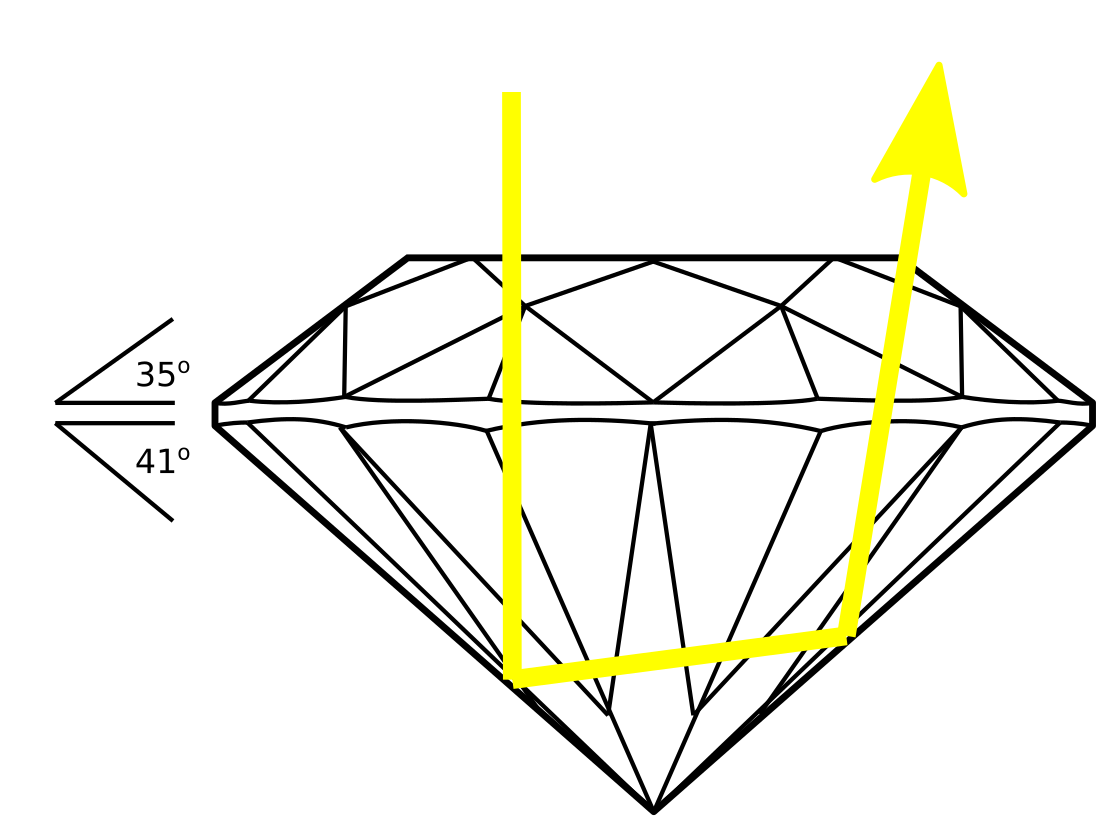
\includegraphics[height=3.7truecm]{slike/04_diamant.png}\qquad
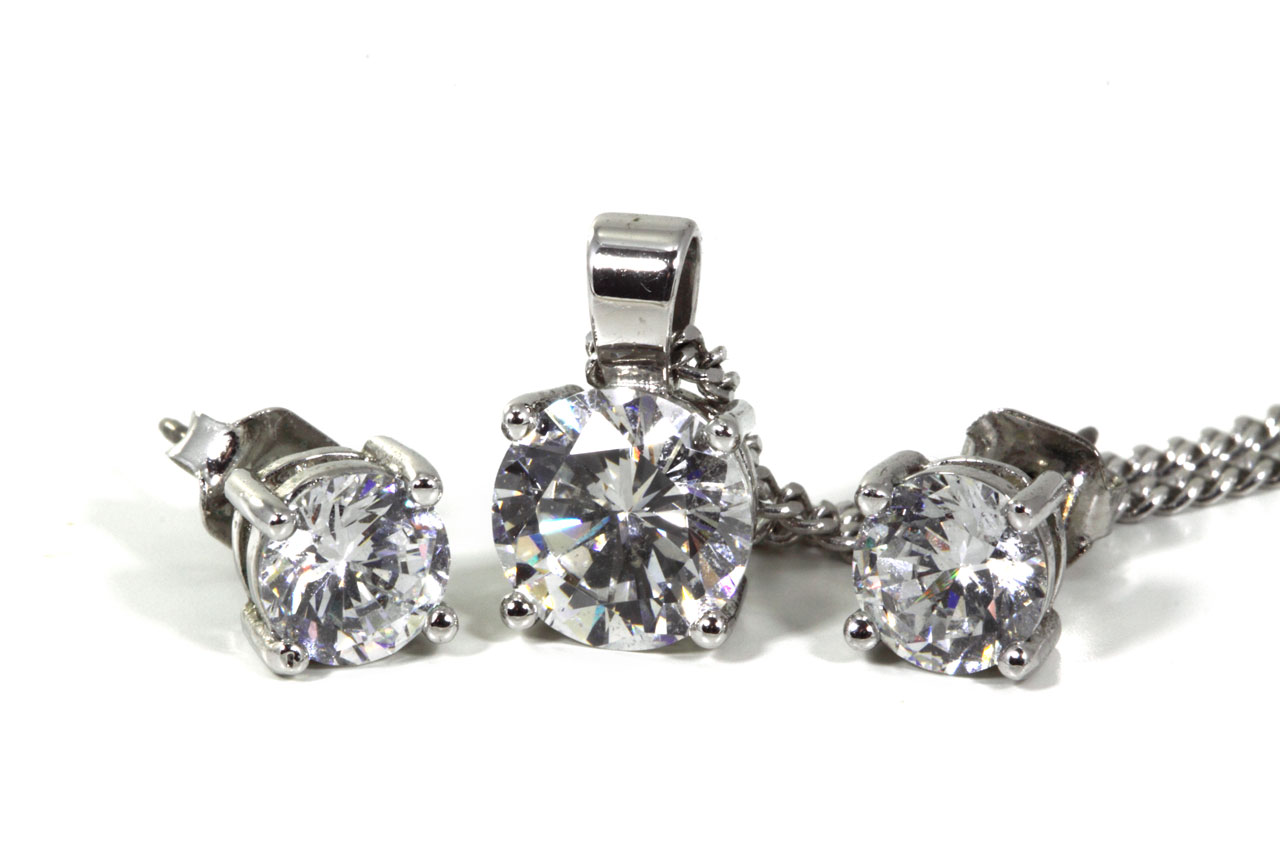
\includegraphics[height=3.7truecm]{slike/04_nakit.jpg}\hfill
\caption{Diamanti so brušeni tako, da se na spodnjih ploskvah vpadna svetloba totalno odbije (levo), 
kar jih naredi še posebej privlačne za nakit. Foto: Vera Kratochvil, PublicDomainPictures.}
\label{fig:04_diamanti}
\vskip-4truemm
\end{figure}
\end{remark}

\section{Evanescento polje}
Povedali smo, da se pri totalnem odboju vsa vpadna svetloba odbije. Izračunajmo
zdaj jakosti električnega polja pri totalnem odboju na obeh straneh meje med snovema.

Naj svetloba vpada na ravno mejo med dvema neprevodnima, homogenima 
in izotropnima snovema, za kateri velja $n_1>n_2$, pod kotom, ki je večji od mejnega
kota totalnega odboja. Amplitudni odbojnosti 
za obe polarizaciji zapišemo kot (enačbi~\ref{eq:04_54} in 
\ref{eq:TMr}):
\begin{equation}
r_{\mathrm{TE}} = \frac{n_1 \cos \alpha - i n_2 \kappa}
{n_1 \cos \alpha + i n_2 \kappa} \qquad \mathrm{in} \qquad
r_{\mathrm{TM}} = \frac{n_2 \cos \alpha - i n_1 \kappa}
{n_2 \cos \alpha + i n_1 \kappa},
\label{eq:04_61}
\end{equation}
pri čemer je $\kappa$ podan z enačbo~(\ref{eq:04_55}).

Poglejmo primer TE polariziranega valovanja. Valovni
vektor prepuščenega valovanja je enak (slika~\ref{fig:04_totalni}\,b):
\begin{equation}
\mathbf{k}_t = \left( k_0 n_2 \sin \beta, 0, k_0 n_2 \cos \beta \right) = 
\left( k_0 n_1 \sin \alpha, 0, i k_0 n_2 \kappa \right)\!.
\label{eq:04_62}
\end{equation}
Pri tem smo za izračun komponente $x$ uporabili lomni zakon (enačba~\ref{eq:04_18}). 
Komponenta $z$ postane pri kotih, ki so večji od mejnega kota totalnega odboja, imaginarna. 
Ustrezno smo namesto $\cos \beta$ zapisali $i\kappa$. 
Prepuščeno valovanje v snovi z manjšim lomnim količnikom 
pri totalnem odboju z upoštevanjem enačbe~(\ref{eq:04_62}) zapišemo kot:
\begin{align}
\mathbf{E}_t &= \mathbf{E}_{0t} e^{i k_0 n_2 x \sin \beta }
 e^{i k_0 n_2 z\cos \beta} e^{-i \omega t} \nonumber\\
 &= \mathbf{e}_{y} E_{0t}  e^{i k_0 n_1 x\sin \alpha}
 e^{-i \omega t} e^{- \varkappa z},
 \label{eq:04_63}
\end{align}
pri čemer smo vpeljali atenuacijski koeficient:\index{Atenuacijski koeficient}
\begin{equation}
\varkappa = k_0 n_2 \kappa.
\label{eq:kappatot}
\end{equation}
Eksponentno pojemajočemu polju v snovi z manjšim 
lomnim količnikom pravimo evanescentno polje\index{Evanescentno polje} 
in ga v realni obliki zapišemo kot:
\begin{equation}
\mathbf{E}_t = \mathbf{e}_{y} E_{0t} e^{- \varkappa z}
\cos \left( k_0 n_1 x\sin \alpha -\omega t\right)\!. 
\label{eq:04_64}
\end{equation}
Valovne fronte evanescentnega polja potujejo v smeri $x$, 
amplituda pa pojema eksponentno v smeri $z$. 

Izračunajmo še odbito polje pri totalnem odboju, ki je  do faze natančno 
enako vpadnemu, le smer $k_z$ se spremeni. Zaenkrat zanemarimo fazni zamik
in polje v snovi z večjim lomnim količnikom zapišemo kot vsoto vpadnega
in odbitega valovanja:
\begin{align}
\mathbf{E}_1 &= \mathbf{e}_{y} E_{0} \left(
e^{ik_0n_1x\sin \alpha}e^{ik_0n_1z\cos \alpha}+
e^{ik_0n_1x\sin \alpha}e^{-ik_0n_1z\cos \alpha }\right) e^{-i \omega t} \nonumber\\
&= 2\mathbf{e}_{y} E_{0} e^{ik_0n_1x\sin \alpha -i\omega t} 
\cos \left(k_0 n_1z\cos \alpha \right).
 \label{eq:04_65}
\end{align}
Realni del celotne jakosti električnega polja v snovi z večjim lomnim 
količnikom je:
\boxeq{eq:ev1}{
\mathbf{E}_1 = 2 \mathbf{e}_{y} E_{0} 
\cos \left(k_0 n_1z\cos \alpha\right)\cdot 
\cos \left(k_0 n_1x\sin \alpha-\omega t\right)
}
in v snovi z manjšim lomnim količnikom:
\boxeq{eq:ev2}{
\mathbf{E}_2 = 2\mathbf{e}_{y} E_{0} 
e^{-\varkappa z} 
\cos \left(k_0 n_1 x \sin \alpha-\omega t\right).
}
Pri tem smo upoštevali zvezo $E_{0t} = 2E_{0i} = 2E_0$, ki sledi neposredno iz 
robnih pogojev pri $z=0$.

Na sliki~\ref{fig:04_simulacija} je prikazana primerjava med valovanjem
pri navadnem lomu in valovanjem pri totalnem odboju. V prvem primeru (levo) se
na vpadni strani pojavi interferenca med
vpadnim in šibkejšim odbitim žarkom, na drugi strani meje pa se prepuščeno valovanje nemoteno
širi. V primeru totalnega odboja (desno) na vpadni strani interferirata 
vpadni in odbiti žarek z enako amplitudo, na drugi strani meje pa polje pojema 
eksponentno z oddaljenostjo od meje med snovema. Valovanje na obeh straneh meje
potuje vzporedno z osjo $x$. 
\begin{figure}[ht]
\centering
\def\svgwidth{140truemm} 
\input{slike/04_sim_lom.pdf_tex}
\caption{Intenziteta valovanja ob 
danem trenutku pri navadnem odboju (levo) in totalnem odboju (desno).
V snovi z manjšim lomnim količnikom ($n_2$) se v prvem primeru svetloba razširja
kot valovanje, v drugem primeru pri večjem vpadnem kotu pa se pojavi eksponentno pojemajoče evanescentno
polje.}
\label{fig:04_simulacija}
\end{figure}

Izračunajmo še Poyntingov vektor\index{Poyntingov vektor} na obeh straneh meje za primer totalnega odboja. 
Račun pokaže, da ima v obeh snoveh Poyntingov vektor samo komponento vzdolž osi $x$,
vzdolž osi $z$ pa ne (glej primer~\ref{primer:04_S}). To pomeni, da se energija pri totalnem odboju širi 
vzdolž meje med snovema, v smeri pravokotno na mejo pa ne.  

\begin{example}{\bf Energijski tok pri totalnem odboju.}
\label{primer:04_S}
Izračunajmo Poyntingov vektor pri totalnem odboju v snovi z manjšim 
lomnim količnikom (snovi 2). Obravnavajmo TE polarizirano valovanje in 
zaradi nazornosti računajmo v realni obliki. Jakost električnega
polja (enačba~\ref{eq:04_64}) potem zapišemo kot:
\begin{equation}
\mathbf{E} = 
E_{0t} e^{-\varkappa z}\cos(k_xx-\omega t)
\left[
\begin{array}{c}
0\\
1\\
0\\
\end{array}
\right]\!\!.
 \label{eq:04_71}
\end{equation}
Jakost magnetnega polja izračunamo iz Maxwellove enačbe (enačba~\ref{eq:Maxwell2}), pri 
čemer se omejimo na nemagnetne snovi:
\begin{equation}
\nabla \times \mathbf{E} = -\mu_0 \frac{\partial \mathbf{H}}{\partial t}.
\label{eq:04_72}
\end{equation}

Najprej izračunamo levo stran enačbe:
\begin{equation}
\nabla \times \mathbf{E} = \left|
\begin{array}{ccc}
\mathbf{e}_x & \mathbf{e}_y & \mathbf{e}_z \\
\frac{\partial}{\partial x} & \frac{\partial}{\partial y} & \frac{\partial}{\partial z} \\
0&E_{0t}e^{-\varkappa z} \cos \left(k_xx-\omega t\right)& 0 \\
\end{array}
\right| = \left[
\begin{array}{c}
\varkappa E_{0t} e^{-\varkappa z} \cos \left(k_xx-\omega t\right) \\
0\\
-k_x E_{0t} e^{-\varkappa z} \sin \left(k_xx-\omega t\right)\\
\end{array}
\right]\!\!.
\label{eq:04_73}
\end{equation}
Sledi:
\begin{equation}
\frac{\partial \mathbf{H}}{\partial t} = \frac{E_{0t} e^{-\varkappa z}}{\mu_0} \left[
\begin{array}{c}
-\varkappa  \cos \left(k_xx-\omega t\right) \\
0\\
k_x \sin \left(k_xx-\omega t\right)\\
\end{array}
\right]\!\!.
\label{eq:04_74}
\end{equation}
Z integracijo po času izračunamo jakost magnetnega polja:
\begin{equation}
\mathbf{H} = \frac{E_{0t}e^{-\varkappa z}}{\mu_0} \left[
\begin{array}{c}
-\varkappa  \int \cos \left(k_xx-\omega t\right) dt\\
0\\
k_x  \int\sin \left(k_xx-\omega t\right) dt\\
\end{array}
\right] = 
\frac{E_{0t}e^{-\varkappa z}}{\mu_0} \left[
\begin{array}{c}
\frac{\varkappa}{\omega}  \sin \left(k_xx-\omega t\right)\\
0\\
\frac{k_x}{\omega} \cos \left(k_xx-\omega t\right)\\
\end{array}
\right]\!\!.
\label{eq:04_75}
\end{equation}
Zdaj lahko izračunamo Poyntingov vektor kot vektorski produkt jakost
električnega in magnetnega polja (enačba~\ref{eq:Poyntingov}):
\begin{equation}
\mathbf{S} = \mathbf{E} \times \mathbf{H} = 
E_{0t}e^{-\varkappa z} \left[ \begin{array}{c}
                        0\\
                        \cos(k_xx-\omega t)\\
                        0 \\
                       \end{array}\right]
\times
\frac{E_{0t}e^{-\varkappa z}}{\mu_0\omega}\left[
\begin{array}{c}
\varkappa \sin \left(k_xx-\omega t\right)\\
0\\
k_x \cos \left(k_xx-\omega t\right) \\
\end{array}
\right]\!\!.
\label{eq:04_76}
\end{equation}
Dobimo:
\begin{equation}
\mathbf{S} 
= \frac{E_{0t}^2}{\mu_0\omega}e^{-2\varkappa z}\left[
\begin{array}{c}
k_x\cos^2 \left(k_xx-\omega t\right)\\
0\\
-\varkappa \sin \left(k_xx-\omega t\right) \cos \left(k_xx-\omega t\right)\\
\end{array}
\right]\!\!.
\label{eq:04_77}
\end{equation}
Pri energijskem toku nas zanima časovno povprečje Poyntingovega vektorja:
\begin{equation}
\langle \mathbf{S}\rangle = \frac{E_{0t}^2}{\mu_0\omega}e^{-2\varkappa z}\left[
\begin{array}{c}
k_x/2\\
0\\
0\\
\end{array}
\right]\!\!.
\label{eq:04_78}
\end{equation}
Iz zapisanega vidimo, da je energijski tok v smeri $z$ enak nič -- pravokotno na mejno 
ploskev se torej energija pri totalnem odboju ne prenaša. 

V smeri vzporedno z mejno ploskvijo je izračunana komponenta Poyntingovega vektorja:
\begin{equation}
\langle \mathbf{S}_x\rangle = \frac{E_{0t}^2}{2\mu_0\omega}e^{-2\varkappa z}k_0 n_1\sin \alpha,
\label{eq:04_79}
\end{equation}
pri čemer smo upoštevali, da je $k_x = k_0 n_1 \sin \alpha$. Izraz v števcu in imenovalcu pomnožimo 
z $\varepsilon_0$, upoštevamo izraz za svetlobno hitrost (enačba~\ref{eq:c0}) in zvezo med krožno frekvenco
in valovnim številom. Dobimo:
\begin{equation}
\langle \mathbf{S}_x\rangle = \frac{1}{2}\varepsilon_0 E_{0t}^2 c_0 n_1  e^{-2\varkappa z} \sin \alpha.
\label{eq:04_80}
\end{equation}
Dobili smo izraz za gostoto svetlobnega toka, ki pa je pomnožen s faktorjem $\sin \alpha$ in seveda eksponentno
pojemajočim delom $\exp(-\varkappa z)$.

Poyntingov vektor lahko izračunamo tudi na vpadni strani meje med snovema. Izračun pokaže, da
je tudi na vpadni strani od nič različno le povprečje komponente $x$, povprečje komponente v smeri $z$ 
pa je enako nič. Za razliko od eksponentnega pojemanja intenzitete v evanescentnem polju, se na
vpadni strani intenziteta spreminja oscilatorno.
\end{example}

Izračunajmo še vdorno globino $d_v$ evanescentnega polja\index{Vdorna globina!{evanescentno polje}}
v snovi z manjšim lomnim količnikom, ki 
jo vpeljemo kot inverz parametra $\varkappa$. Spomnimo se, da je parameter $\varkappa$ za TE polarizirano
valovanje enak (enačba~\ref{eq:kappatot}):
\begin{equation}
\varkappa = k_0 n_2 \kappa = k_0 n_2 \sqrt{\left(\frac{\sin \alpha}{\sin \alpha_m}\right)^2-1}.
\label{eq:04_81}
\end{equation}
Vdorna globina je potem:
\begin{equation}
d_v = \frac{1}{\varkappa} = \frac{\lambda_0}{2 \pi n_2 }\frac{1}{\sqrt{\left(\frac{\sin \alpha}{\sin \alpha_m}\right)^2-1}}=
\frac{\lambda_0}{2\pi}\frac{1}{\sqrt{n_1^2\sin ^2\alpha - n_2^2}}.
\label{eq:04_82}
\end{equation}
Odvisnost vdorne globine od vpadnega kota je prikazana na sliki~\ref{fig:04_vdorna}. Po pričakovanju
se pri $\alpha = \alpha_m$ vdorna globina povečuje proti neskončnosti, saj totalni odboj 
preide v navaden lom, pri katerem je doseg v idealnem primeru neskončen. Pri $\alpha \to \pi/2$ vdorna
globina pade na vrednost $d_v = \lambda_0/2\pi \sqrt{n_1^2-n_2^2}$.
\begin{figure}[ht]
\centering
\def\svgwidth{80truemm} 
\input{slike/04_vdorna.pdf_tex}
\caption{Odvisnost vdorne globine $d_v$ od vpadnega kota $\alpha$}
\label{fig:04_vdorna}
\end{figure}

\begin{remark}
Celotna obravnava evanescentnega polja je bila narejena za TE polarizirano valovanje. Za TM polarizirano
valovanje je postopek povsem analogen in tudi rezultati so podobni. Razlikuje se le vrednost
parametra $\varkappa$, ki je za TM valovanje:
\begin{equation}
\varkappa_\mathrm{TM} = k_0 n_1 \kappa.
\label{eq:kappatottm}
\end{equation}
\end{remark}

\subsection*{Frustrirani totalni odboj}\index{Totalni odboj!frustrirani}
Izračunali smo evanescentno polje, to je električno polje, ki se pojavi pri totalnem odboju
v snovi z manjšim lomnim količnikom. Pri tem smo privzeli, da je snov v smeri pravokotno
na mejno ploskev neomejena. 

Postavimo zdaj za to snov plast tretje snovi. Mejni ploskvi naj bosta vzporedni, lomni 
količnik tretje snovi pa naj ima večji lomni količnik kot vmesna snov. Če je debelina
vmesne plasti razmeroma majhna, lahko pride to tuneliranja\index{Tuneliranje}
svetlobe iz vrhnje v spodnjo snov
(slika~\ref{fig:04_tunel}). To je še zlasti opazno, kadar je debelina vmesne snovi po 
velikosti primerljiva z vdorno globino evanescentnega polja. Takrat
znaten delež vpadne svetlobe preide v spodnjo snov. Prepustnost takega ``tunela'' za svetlobo 
spreminjamo z debelino vmesne plasti ali s spreminjanjem vpadnega kota.
\begin{figure}[ht]
\centering
\def\svgwidth{60truemm} 
\input{slike/04_tunel.pdf_tex}
\caption{Kadar je debelina vmesne plasti z lomnim količnikom, ki je manjši od lomnega količnika
zgornje in spodnje plasti ($n_1>n_2<n_3$), majhna v primerjavi z vdorno globino svetlobe, 
svetloba tunelira skozi tanko plast. }
\label{fig:04_tunel}
\end{figure}
\begin{remark}
Na podlagi frustriranega totalnega odboja delujejo optični čitalci prstnih odtisov. Pri 
navadnem totalnem odboju se vsa svetloba odbije. Kadar je totalni odboj frustriran, se 
odbije le del svetlobe, del pa je prepuščen, pri čemer je intenziteta odbite
svetlobe močno odvisna od širine vmesne tanke plasti. Ko prst prislonimo ob plast,
na kateri prihaja do totalnega odboja, se zaradi drobnih vdolbin v vzorcu na prstih
svetloba ponekod močno odbija, drugod pa šibkeje. Intenziteta odbite svetlobe
tako poda sliko prstnega odtisa.
\end{remark} 

\begin{figure}[ht]
\centering
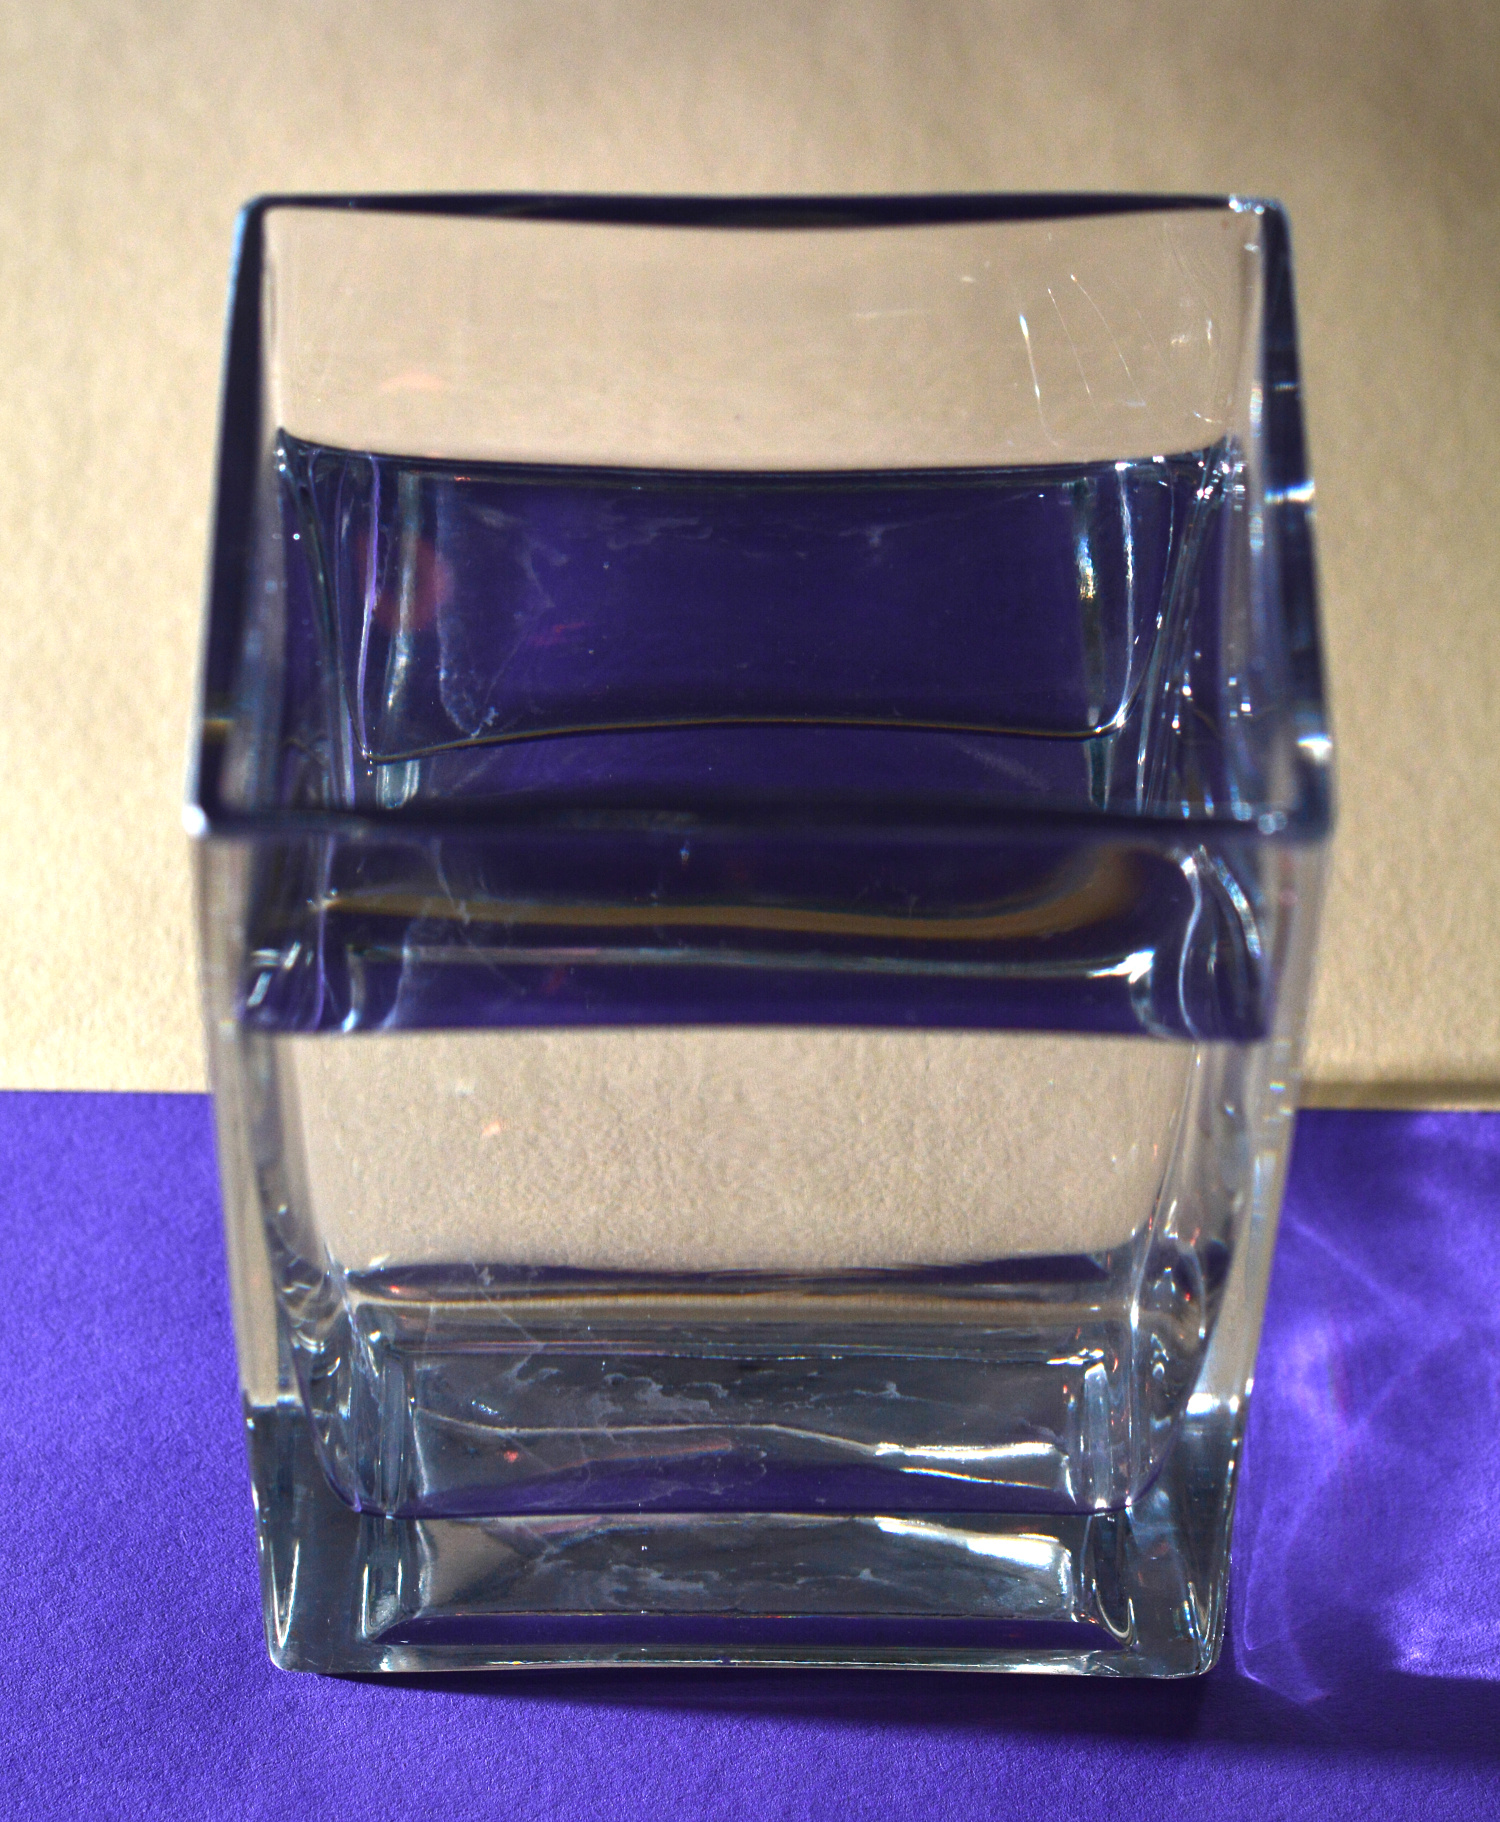
\includegraphics[width=5.5truecm]{slike/04_TIRF1.jpg}\qquad \qquad
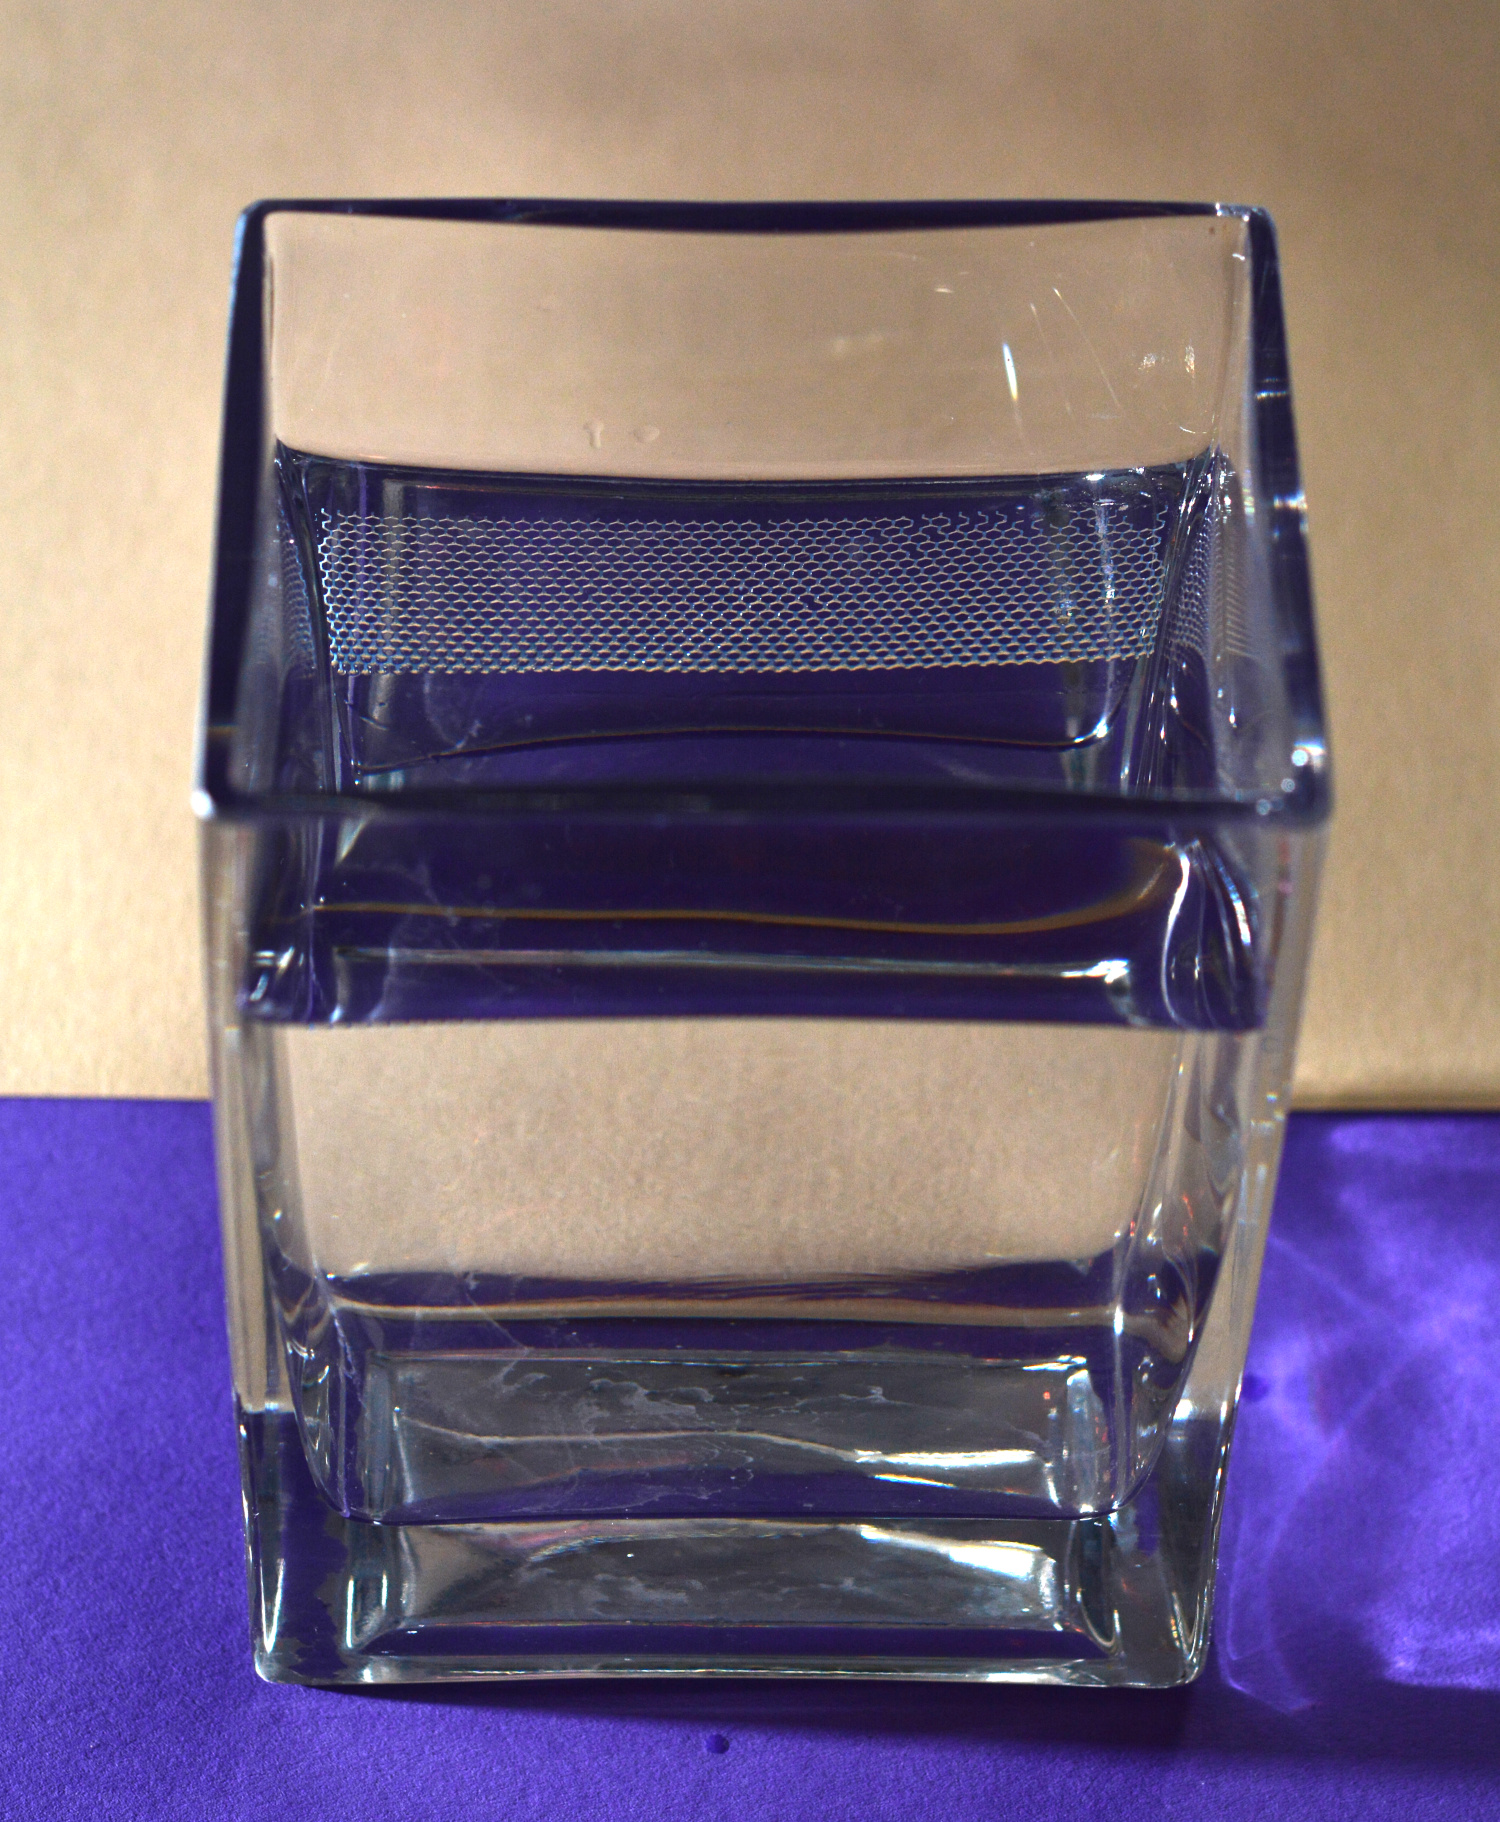
\includegraphics[width=5.5truecm]{slike/04_TIRF2.jpg}
\caption{Svetloba se ob prehodu iz vode v zrak na zadnji steni steklene vaze 
totalno odbije, zato tam vidimo vijolično dno (levo). Ko ob zadnjo steno prislonimo
navlaženo mrežasto tkanino, na mestih stika totalnega odboja ni več in svetloba prehaja
skozi mejo kljub vpadnemu kotu, večjemu od mejnega kota totalnega odboja (desno).}
\label{fig:04_FTIRfoto}

\end{figure}
\begin{remark}
Pri totalnem odboju se zgodi še en zanimiv pojav, ki ga imenujemo Goose--H\"anchen pojav 
po nemških fizikih Hermannu Fritzu Gustavu Goosu (1883--1968) in Hildi H\"anchen 
(1919--2013).\index{Goos--H\"anchen pojav}\index{Goos, Fritz}\index{H\"anchen, Hilda}
Ko se linearno polarizirana svetloba totalno odbije, odbita svetloba ne izhaja iz 
povsem iste točke, kot nanjo vpada. Videti je, kot da se svetloba odbije od neke 
navidezne ravnine, ki leži v snovi z manjšim lomnim količnikom (slika~\ref{fig:04_Goos}). 
Oddaljenost te navidezne odbojne ravnine je kar enaka vdorni globini, 
zato je vzporeden premik enak: $L = 2d_v\,\tan(\alpha)$.

Pojava z opisom poti enega žarka svetlobe ne moremo pojasniti, temveč moramo
obravnavati snop svetlobe, sestavljen iz več žarkov. Žarki vpadajo na mejo pod rahlo
različnimi vpadnimi koti, zato imajo po odboju rahlo različno fazo. Skupni 
učinek faznih zakasnitev je tak, kot bi se žarek navidezno vzdolžno premaknil. 
\begin{figure}[ht]
\centering
\def\svgwidth{70truemm} 
\input{slike/04_Goos.pdf_tex}
\caption{Goos-H\"anchen pojav pri totalnem odboju: totalno odbita svetloba izhaja iz druge točke, 
kot vpadna svetloba vpada na mejo snovi. Videti je, kot da se odbije od navidezne ravnine.}
\label{fig:04_Goos}
\vglue-5truemm\end{figure}
\end{remark}

\section{Faza pri totalnem odboju}\index{Faza pri totalnem odboju}\index{Totalni odboj!faza}\index{Faza pri odboju}
Poglejmo še, kaj se zgodi s fazo valovanja pri odboju na meji med dvema snovema. 
Pri navadnem odboju, pri katerem sta koeficienta
amplitudne odbojnosti za obe polarizaciji realna, ni težav. 
Pogledati moramo samo predznak $r$ v Fresnelovih enačbah (enačbi~\ref{eq:TEr} 
in \ref{eq:TMr}). Pri odboju na 
optično gostejšem sredstvu se faza TE polariziranega valovanja 
spremeni za $\pi$, faza TM polariziranega
valovanja pa pri Brewstrovem kotu preskoči s $\pi$ na 0. 
Pri vpadu na optično redkejšo snov se faza
TE polarizacije ohranja, faza TM polarizacije pa pri 
Brewstrovem kotu preskoči z 0 na $\pi$.  

Zanimivejša je faza pri totalnem odboju. V prejšnjem razdelku smo spoznali atenuacijski 
koeficient\index{Atenuacijski koeficient}
$\varkappa$, ki je močno odvisen od vpadnega kota in tudi od polarizacije 
valovanja (enačbi~\ref{eq:kappatot} 
in \ref{eq:kappatottm}):
\begin{equation}
\varkappa_{\mathrm{TE}}= k_0 n_2 \sqrt{\left(\frac{\sin \alpha}{\sin \alpha_m}\right)^2-1} 
\qquad \mathrm{in}\qquad
\varkappa_{\mathrm{TM}}= k_0 n_1 \sqrt{\left(\frac{\sin \alpha}{\sin \alpha_m}\right)^2-1}.
\label{eq:04_83}
\end{equation}
Valovanje v obliki evanescentnega valovanja vdira v snov z manjšim lomnim količnikom, zato
pri odboju pridobi fazni zamik. Ker je fazni zamik neposredno povezan z atenuacijskim
koeficientom oziroma vdorno globino, je odvisen od vpadnega kota $\alpha$ in polarizacije svetlobe. 

Izračunajmo najprej fazo za TE polarizirano valovanje.
Izhajamo iz amplitudne odbojnosti (enačba~\ref{eq:04_61})
in kompleksni števili v števcu in imenovalcu zapišemo v polarni obliki:
\begin{equation}
r_\mathrm{TE} = \frac{n_1 \cos \alpha - i n_2 \kappa}{n_1 \cos \alpha + i n_2 \kappa} = 
\frac{\sqrt{n_1^2\cos^2 \alpha + n_2^2 \kappa^2}\,e^{-i\delta_\mathrm{TE}/2}}{\sqrt{n_1^2\cos^2 \alpha + n_2^2 \kappa^2}\,e^{+i\delta_\mathrm{TE}/2}}
= e^{-i\delta_\mathrm{TE}},
\label{eq:04_84}
\end{equation}
pri čemer je:
\begin{equation}
\delta_\mathrm{TE} = 2\arctan\frac{n_2\kappa}{n_1 \cos \alpha} = 2\arctan\frac{n_2 \sqrt{\left(\frac{\sin \alpha}{\sin \alpha_m}\right)^2-1}}{n_1 \cos \alpha} = 
2\arctan\frac{\sqrt{n_1^2\sin^2 \alpha-n_2^2}}{n_1 \cos \alpha}.
\label{eq:04_85}
\end{equation}
Fazni zamik totalno odbitega valovanja je torej odvisen od vpadnega kota $\alpha$. 
Pri $\alpha = \alpha_m$ je vrednost $\delta=0$, pri vpadnem kotu $\alpha \to 90\si{\degree}$ pa je
fazni zamik odbitega valovanja $\delta = \pi$. Vmesna odvisnost je prikazana na sliki~\ref{fig:04_faza}.
\begin{figure}[ht]
\centering
\def\svgwidth{80truemm} 
\input{slike/04_faza.pdf_tex}
\caption{Fazna zamika totalno odbite svetlobe in 
njuna razlika $\Delta$ v odvisnosti od vpadnega kota $\alpha$ za obe polarizaciji. Izračun 
je narejen za $n_1 = 2$ in $n_1 = 1$.}
\label{fig:04_faza}
\end{figure}

Podoben rezultat dobimo tudi za TM polarizirano valovanje, le da sta lomna količnika $n_1$ in $n_2$
zamenjana. Tako velja:
\begin{equation}
\delta_\mathrm{TM}= 2\arctan\frac{n_1\kappa}{n_2 \cos \alpha} = 2\arctan\frac{n_1 \sqrt{\left(\frac{\sin \alpha}{\sin \alpha_m}\right)^2-1}}{n_2 \cos \alpha}.
\label{eq:04_86}
\end{equation}
Ker je predpogoj za totalni odboj $n_1 > n_2$, so vrednosti faznega zamika za 
TM polarizacijo vedno večje od faznega zamika za TE polarizirano
valovanje. 

Velja namreč:
\begin{equation}
\tan \frac{\delta_\mathrm{TM}}{2} = \left(\frac{n_1}{n_2}\right)^2 \tan \frac{\delta_\mathrm{TE}}{2}
\label{eq:04_87}
\end{equation}
in posledično:
\begin{equation}
\Delta = \delta_\mathrm{TM}-\delta_\mathrm{TE} \ge 0.
\label{eq:04_88}
\end{equation}
Če je razmerje lomnih količnikov dovolj veliko, je lahko  razlika faznih zamikov 
večja od $\pi/4$. To se, na primer, lahko zgodi pri totalnem odboju na meji med steklom in zrakom. 
Kadar je fazna razlika med obema polarizacijama pri odboju tako velika, lahko  z dvema zaporednima
totalnima odbojema pri nekem vpadnem kotu $\alpha$
dosežemo fazni zamik med TE in TM polariziranim valovanjem, ki je enak $\pi/2$. 
Optični element, v katerem pride do dveh zaporednih totalnih odbojev, torej lahko deluje kot ploščica
$\lambda/4$.\index{Ploščica $\lambda/4$}
S štirimi totalnimi odboji dobimo fazni zamik $\pi$ in učinek ploščice 
$\lambda/2$.\index{Ploščica $\lambda/2$} 
Tovrstni optični elementi se imenujejo Fresnelovi rombi 
(slika~\ref{fig:04_Fresneltot}).\index{Fresnelov romb} 
Njihova glavna prednost je v tem, da delujejo neodvisno od 
valovne dolžine $\lambda$, saj ta ne nastopa eksplicitno v izrazu za $\Delta$. Popravke 
višjega reda, na primer odvisnost lomnega količnika od valovne dolžine, tukaj zanemarimo.
\begin{figure}[ht]
\centering
\def\svgwidth{70truemm} 
\input{slike/04_Fresneltot.pdf_tex}
\caption{V Fresnelovem rombu se vpadna svetloba dvakrat totalno odbije, pri čemer
se med polarizacijama pojavi zamik $\pi/2$. Iz vpadne linearne polarizacije pod kotom 
$45\si{\degree}$ nastane krožno polarizirano valovanje in Fresnelov romb deluje 
kot ploščica $\lambda/4$. Romb je narejen tako, da je iskani fazni 
zamik dosežen pri pravokotnem vpadu na vstopno ploskev.}
\label{fig:04_Fresneltot}
\end{figure}

\section{Odboj na kovinah}
\label{section:410}\index{Odboj na kovinah}
Zanimivo vprašanje je, kako se Fresnelove enačbe spremenijo, če je snov, 
na katero svetloba vpada, prevodna. V tem primeru
vemo, da polje pojema z globino zaradi notranjih električnih tokov. 
Po analogiji s totalnim odbojem, pri katerem evanescentno polje prav tako
pojema z globino, pričakujemo, da bo odbojnost na meji velika. 

Ker je zaradi meje simetrija prostora zlomljena le v smeri osi $z$, polje
lahko pojema le z globino, to je s koordinato $z$. 
Omejimo se zaenkrat na TE polarizirano valovanje, ki 
ga v prevodni snovi zapišemo kot:
\begin{equation}
\mathbf{E}_2 = \mathbf{e}_y E_{0t} e^{i(k_z+i\varkappa)z} e^{ik_xx-i\omega t}.
\label{eq:04_89}
\end{equation}
Komponenta valovnega vektorja, ki je vzporedna z mejno ploskvijo, je zaradi
robnih pogojev enaka na obeh straneh meje. Zapišemo jo kot: $k_x = k_0 n_1 \sin \alpha$. 

Za opis valovanja v prevodni snovi moramo namesto valovne enačbe uporabiti telegrafsko enačbo 
(enačba~\ref{eq:telegrafska}). Kompleksno valovno število izrazimo s\index{Valovni vektor!kompleksni}
\index{Lomni količnik!kompleksni}
kompleksnim lomnim količnikom $\mathcal{N}$ (enačba~\ref{eq:nkompleks2}):
\begin{equation}
|\tilde{\mathbf{k}}|^2 = k_x^2 + (k_z+i\varkappa)^2 = k_0^2 \mathcal{N}^2  = 
k_0^2 \left(\varepsilon_2 + \frac{i\sigma_2}{\varepsilon_0 \omega}\right)\!\!,
\label{eq:04_90}
\end{equation}
pri čemer $\epsilon_2$ in $\sigma_2$ označujeta dielektričnost in električno
prevodnost druge (prevodne) snovi. Iz tega sledi:\index{Električna prevodnost}
\begin{equation}
\frac{k_x^2+k_z^2 - \varkappa^2}{k_0^2} + \frac{2 i \varkappa k_z}{k_0^2} = \varepsilon_2 + 
\frac{i \sigma_2}{\varepsilon_0 \omega}.
\label{eq:04_91}
\end{equation}
Parametra $k_z$ in $\varkappa$ izračunamo iz enačbe:
\begin{equation}
k_z^2 - \varkappa^2+ 2 i \varkappa k_z= k_0^2 \varepsilon_2 - k_x^2 + i\frac{k_0^2\sigma_2}{\varepsilon_0 \omega}.
\label{eq:04_92}
\end{equation}
Postopamo podobno kot pri izračunu kompleksnega lomnega količnika in dobimo:
\begin{equation}
k_z^2 = \frac{1}{2}\left(\sqrt{\left(k_0^2\varepsilon_2-k_x^2\right)^2 + \left(\frac{\sigma_2 k_0^2}{\varepsilon_0 \omega}\right)^2}
+ k_0^2\varepsilon_2-k_x^2 \right)
\label{eq:04_93}
\end{equation}
ter
\begin{equation}
\varkappa^2 = \frac{1}{2}\left(\sqrt{\left(k_0^2\varepsilon_2-k_x^2\right)^2 + \left(\frac{\sigma_2 k_0^2}{\varepsilon_0 \omega}\right)^2}
- k_0^2\varepsilon_2+k_x^2\right)\!\!.
\label{eq:04_94}
\end{equation}
Celotno komponento valovnega vektorja v smeri $z$ v prevodni snovi potem zapišemo kot vsoto 
realnega in imaginarnega dela:
\begin{equation}
\tilde{k}_z = k_z + i \varkappa.
\label{eq:04_95}
\end{equation}
Zapišimo robne pogoje, po katerih se ohranjata tangentni komponenti jakosti
električnega in magnetnega polja (enačbi~\ref{eq:RPE} in \ref{eq:RPH}). Prva enačba
je preprosta:
\begin{equation}
E_{0i} + E_{0r} = E_{0t}.
\label{eq:04_97}
\end{equation}
Drugo enačbo dobimo z upoštevanjem Faradayevega zakona (enačba~\ref{eq:Maxwell2}).
Izvrednotimo časovni odvod magnetnega polja in dobimo zvezo: $\nabla \times \mathbf{E}
= i \omega \mu_0 \mathbf{H}$. Na meji se ohranja tangentna komponenta $H_x$ (glej
sliko~\ref{fig:04_tetm}), zato
se na meji ohranja odvod jakosti električnega polja $dE/dz$:
\begin{equation}
-ik_{1z}E_{0i} + ik_{1z}E_{0r}= -(ik_{2z}+\varkappa)E_{0t}.
\label{eq:04_98}
\end{equation}
Eliminiramo neznanko $E_{0t}$ in izračunamo amplitudno odbojnost:
\boxeq{eq:Kovinar}{
r = \frac{E_{0r}}{E_{0i}} = \frac{k_{1z}-k_{2z}-i \varkappa}{k_{1z}+k_{2z}+i\varkappa}.
}
Tak rezultat je pričakovan. Spomnimo se amplitudne odbojnosti za navadni neprevodni primer
(enačba~\ref{eq:TEr}):
\begin{equation}
r = \frac{n_1 \cos \alpha - n_2 \cos \beta}{n_1 \cos \alpha + n_2 \cos \beta} = 
\frac{k_0 n_1 \cos \alpha - k_0 n_2 \cos \beta}{k_0 n_1 \cos \alpha + k_0 n_2 \cos \beta} = 
\frac{k_{1z}-k_{2z}}{k_{1z}+k_{2z}}.
\label{eq:04_96}
\end{equation}
V primeru prevodne snovi je izraz povsem enak, le da namesto
realne vrednosti komponente valovnega vektorja v drugi snovi $k_{2z}$ 
upoštevamo kompleksno vrednost komponente $\tilde{k}_z = k_{2z}+ i\varkappa$. Realni del 
je tako enak kot v neprevodnih snoveh, imaginarni del pa je enak kot pri totalnem odboju
na meji dveh neprevodnih snovi (enačba~\ref{eq:04_54}). 
Temu ustrezno lahko rezultat razumemo kot neko vmesno rešitev, ki delno spominja
na navadni odboj, vendar ima večjo odbojnost. Kovine zato dobro odbijajo svetlobo
in se ``bleščijo''. 
 
Zapišimo amplitudno odbojnost za TE polarizirano valovanje še drugače:\index{Fresnelove enačbe}
\index{Amplitudna odbojnost!{na kovinah}}
\boxeq{eq:04_99}{
r_\mathrm{TE} = \frac{n_1 \cos \alpha - \mathcal{N}_2 \cos
\beta}{n_1 \cos \alpha + \mathcal{N}_2 \cos \beta}.
}
Pri tem je $\cos \beta$ kompleksno število, določeno formalno 
z lomnim zakonom $n_1 \sin \alpha = \mathcal{N}_2 \sin \beta$.
Sklepamo, da po analogiji amplitudno odbojnost za TM polarizirano valovanje zapišemo kot: 
\boxeq{eq:04_100}{
r_\mathrm{TM} = \frac{\mathcal{N}_2 \cos \alpha - n_1
\cos \beta}{\mathcal{N}_2 \cos \alpha + n_1 \cos \beta}.
}

Odbojnost $\mathcal{R}$, ki jo izračunamo kot:\index{Odbojnost!{na kovinah}}
\begin{equation}
\mathcal{R} = |r|^2,
\label{eq:04_100a}
\end{equation}
je prikazana na sliki~\ref{fig:04_kovina}. Odbojnost za TE polarizacijo
homogeno narašča z naraščajočim vpadnim kotom 
od neke začetne vrednosti pri pravokotnem vpadu do 1. 
Intenziteta TM polarizacije na prevodnih snoveh 
nikoli ne pade na nič, se pa pri določenih kotih občutno
zmanjša (analog Brewsterjevem kotu pri odboju na neprevodnih snoveh).
\begin{figure}[ht]
\centering
\def\svgwidth{70truemm} 
\input{slike/04_kovinaMo.pdf_tex}
\caption{Odbojnost na prevodni snovi v odvisnosti od vpadnega kota za TE in TM polarizirano\index{Molibden}
valovanje. Primer je narisan za molibden z $n'=3,70$ in $n''=3,55$, pri čemer je $\mathcal{N} = n'+in''$.}
\label{fig:04_kovina}
\end{figure}

Račun odboja na kovini je razmeroma zapleten. Preprost je le v primeru pravokotnega vpada, 
ko sta $\alpha = \beta = 0$. Takrat dobimo za amplitudno odbojnost:
\begin{equation}
r = \frac{n_1 - \mathcal{N}}{n_1 + \mathcal{N}} = \frac{n_1 -n_2' -in_2''}{n_1 +n_2' +in_2''},
\label{eq:04_101}
\end{equation}
pri čemer $n_2'$ označuje realni in $n_2''$ imaginarni del kompleksnega lomnega količnika.
Izračunamo še odbojnost:
\begin{equation}
\mathcal{R} = |r|^2 = \frac{(n_1 -n_2')^2 +n_2''^2}{(n_1 +n_2')^2 +n_2''^2}.
\label{eq:04_102}
\end{equation}
Kadar je realni del $n'$ lomnega količnika zelo majhen, lahko izraz še poenostavimo 
in dobimo:
\begin{equation}
\mathcal{R} = \frac{n_1^2 +n_2''^2}{n_1^2 +n_2''^2} = 1.
\label{eq:04_103}
\end{equation}
Snovi z majhnim realnim delom lomnega količnika $n'$ torej vso vpadno 
svetlobo odbijejo. Primera takih kovin sta srebro ($n'=0,15$ in $n''=3,9$)\index{Srebro}
in aluminij ($n'=1,3$ in $n''=7,3$). Obe kovini zato uporabljamo za izdelavo\index{Aluminij}
zrcal.
\begin{figure}[ht]
\centering
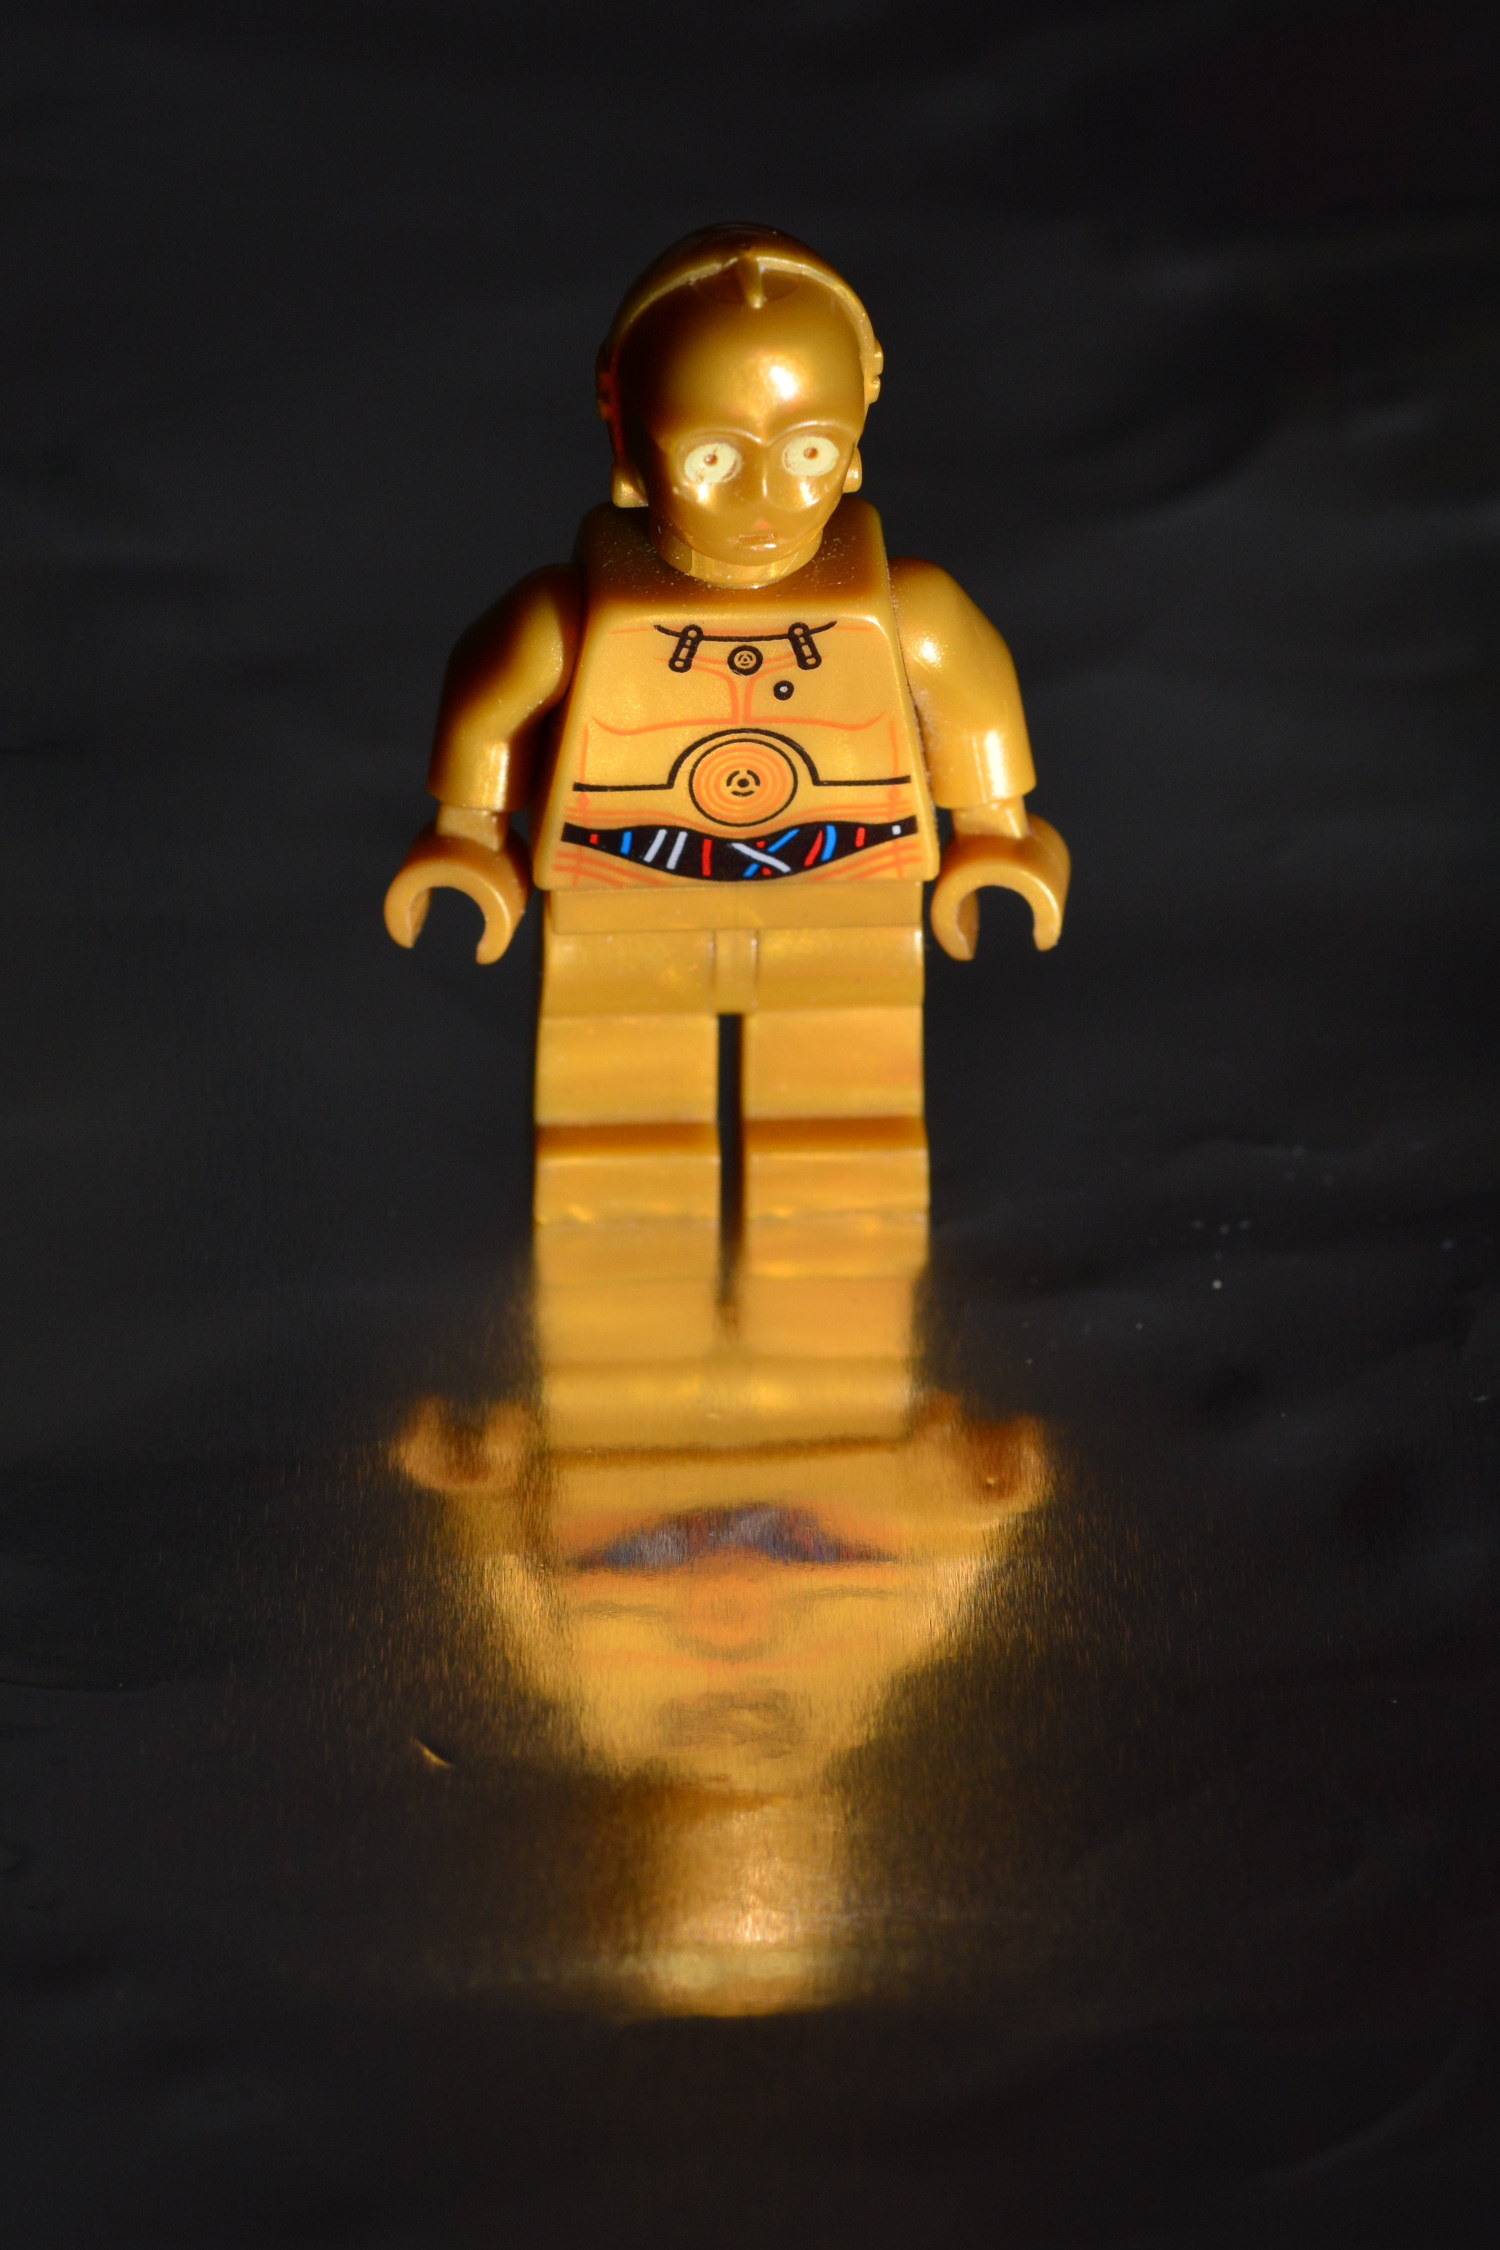
\includegraphics[width=6truecm]{slike/04_photos_kovina.jpg}
\caption{Gladka površina dobro prevodnih kovin odbija praktično 
vso vpadno svetlobo, zato jih uporabljamo za izdelavo zrcal. Kuhinjska aluminijasta
folija na sliki ni povsem gladka, zato je zrcalna slika popačena.}
\label{fig:04_KovinaFoto}
\end{figure}

%\chapterimage{Geometrijska.jpg} % Chapter heading image

\chapter{Uklon}
V tem poglavju bomo spoznali enega najznačilnejših pojavov valovne 
optike -- uklon. Zapisali bomo splošni uklonski integral in obravnavali
dva približka, Fraunhoferjevega in Fresnelovega. Z izračunom 
bomo pojasnili značilne uklonske slike in zapisali uklonsko
omejeno ločljivost optičnih naprav. Na koncu poglavja sledi matematično
zahtevnejša izpeljava Kirchhoffovega uklonskega integrala. 

\section{Uklonski integral}
Svetloba se uklanja, kadar vpada na oviro, katere velikost je primerljiva z valovno  
dolžino svetlobe, ali se širi skozi podobno veliko odprtino v zaslonu. 
V geometrijski optiki se svetloba širi po ravnih črtah, ki po 
najkrajši poti povezujejo začetno in končno točko. V tej sliki za oviro 
nastane ostra senca, v katero se svetloba ne širi. Po uklonski teoriji
svetloba seže deloma tudi v območje sence. Poleg tega, da se valovanje širi
v območje geometrijske sence za ovirami, se v njem pojavijo ojačitve
in oslabitve, ki predstavljajo značilne uklonske slike.

Naj ravno sinusno potujoče valovanje vpada na zaslon, v katerem je majhna odprtina.
Ta zaslon imenujemo objektni zaslon. Iščemo uklonsko sliko, ki nastane
za odprtino na tako imenovanem opazovalnem zaslonu (glej sliko~\ref{fig:05_shema}).
Pri tem  zanemarimo vektorsko naravo polja oziroma
polarizacijo in jakost električnega polja obravnavamo kot skalarno količino.

\begin{figure}[ht]
\centering
\def\svgwidth{90truemm} 
\input{slike/05_skica01.pdf_tex}
\caption{Ravni valovi vpadajo na objektni zaslon, v katerem je odprtina. 
Na opazovalnem zaslonu v točki $P_0$ opazujemo jakost električnega polja v
odvisnosti od vpadnega polja v točki $P$.}
\label{fig:05_shema}
\end{figure}

Naša naloga je poiskati jakost električnega polja v točki $P_0$ na opazovalnem zaslonu, 
do katere vodi vektor $\mathbf{r}_0$, v odvisnosti od vrednosti polja v točki $P$
na objektnem zaslonu, do katerega vodi vektor $\mathbf{r}$.

Po Huygensovem načelu iz vsake točke $P$ v odprtini izhaja sekundarno krogelno valovanje, 
katerega amplitudo določa polje, ki vpada na objektni zaslon. Če je vpadno valovanje
ravni val, velja $E(\mathbf{r}) = E_0$ za vsak $\mathbf{r}$. Za nastanek slike
v točki $P_0$  na opazovalnem zaslonu seštejemo prispevke sekundarnih
polj iz vseh točk odprtine v objektnem zaslonu. 

Uklonsko sliko v točki $P_0$ tako z enačbo zapišemo kot:
\boxeq{eq:05_01}{
E_{P0} = E (\mathbf{r}_0) = \int_A \frac{i}{\lambda} E_0~\frac{e^{ikR(\mathbf{r})}}{R(\mathbf{r})}~ dS,
}
pri čemer integriramo po celotni površini odprtine $A$. Ulomek v integralu predstavlja
krajevni del krogelnih valov, $\lambda$ pa je valovna dolžina vpadne svetlobe. Predfaktor
v obliki $i/\lambda$ bomo izpeljali v razdelku~\ref{chap:Kirchhoff}.
\begin{remark}
Uklonski integral je prvotno zapisal Fresnel, vendar je namesto predfaktorja 
$i/\lambda$ uvedel eksperimentalno določeno konstanto. Predfaktor $i/\lambda$ je 
izpeljal Kirchhoff. Popolnejši zapis predfaktorja je oblike $i \chi(\mathbf{r})/\lambda$,
pri čemer $\chi$ predstavlja smerni faktor. Kadar je značilna razsežnost odprtine v 
objektnem zaslonu $d$ bistveno manjša od oddaljenosti do opazovalnega zaslona, 
je $\chi \approx 1$ in predfaktor se prevede na zapisano obliko. 
\end{remark}

Namesto integracije sekundarnega valovanja po območju odprtine $A$, lahko vpeljemo
tako imenovano aperturno funkcijo $f(\mathbf{r})$. Njena vrednost je na mestu odprtine enaka $1$,
sicer je enaka $0$. Zapis z aperturno funkcijo omogoči integracijo po celotni dvodimenzionalni
ploskvi, ki opisuje objektni zaslon. Zapis je uporaben tudi za splošen primer, ko je zaslon
delno prozoren in le delno prepušča svetlobo. Polje v ravnini objektnega zaslona potem zapišemo kot:
\beq
E(\mathbf{r}) = f(\mathbf{r})E_0.
\label{eq:05_02}
\eeq
Določimo koordinatni sistem na objektni in opazovalni ravnini, ki ju bomo potrebovali
za izračun uklonskega integrala. Objektno ravnino
opišemo kot ravnino s koordinatama $x$ in $y$, vzporedno opazovalno ravnino pa kot ravnino
s koordinatama $\xi$ in $\eta$. Izhodišči obeh koordinatnih sistemov naj ležita 
na skupni osi $z$, ki jo imenujemo optična os sistema (glej sliko~\ref{fig:05_koordinate})
in je pravokotna na obe ravnini.
\begin{figure}[ht]
\centering
\def\svgwidth{120truemm} 
\input{slike/05_koordinate.pdf_tex}
\caption{Optična os sistema (os $z$) povezuje središči obeh ravnin, objektne ($x,y$) in 
opazovalne ($\xi, \eta$). Razdalja med točko v odprtini $P$ in točko na opazovalnem zaslonu $P_0$
je $R$.}
\label{fig:05_koordinate}
\end{figure}

Točko $P$ na objektnem zaslonu opišemo s krajevnim vektorjem:
\beq
P: \mathbf{r} = (x,y,0),
\label{eq:05_03}
\eeq
točko $P_0$ na opazovalnem zaslonu pa s krajevnim vektorjem:
\beq
P_0: \mathbf{r}_0 = (\xi,\eta,z_0).
\label{eq:05_04}
\eeq
Uporabimo uklonski integral (enačba~\ref{eq:05_01}) in zapišemo:
\boxeq{eq:05_05}{
E(\xi, \eta, z_0) = \frac{i}{\lambda} \int_{-\infty}^{\infty}
\int_{-\infty}^{\infty} f(x,y) E_0~\frac{e^{ikR}}{R}~ dx\,dy.
}
V izrazu za krogelne valove nastopa razdalja $R$ med točkama $P$ in $P_0$, za
katero velja:
\beq
R = \sqrt{(\xi-x)^2 + (\eta - y)^2 + z_0^2}.
\label{eq:05_06}
\eeq

Natančna obravnava uklonskega integrala je zelo zahtevna, zato se poslužujemo približkov.
Glede na to, kako natančno obravnavamo izraz za $R = R(x,y,\xi, \eta, z_0)$ v uklonskem
integralu (enačba~\ref{eq:05_05}), ločimo med različnimi uklonskimi približki. Najbolj 
znana sta Fraunhoferjev in Fresnelov približek.

\section{Fraunhoferjev uklon}
O Fraunhoferjevem uklonu oziroma natančneje Fraunhoferjevem uklonskem približku govorimo,
kadar razdaljo $R$ med točko v odprtini in točko na zaslonu v uklonskem integralu 
(enačba~\ref{eq:05_05}) razvijemo do prvega reda. Zapišemo:
\beq
R = \sqrt{(\xi-x)^2 + (\eta - y)^2 + z_0^2} =
\sqrt{\xi^2+\eta^2 +z_0^2 - 2\xi x - 2 \eta y + x^2 + y^2}.
\label{eq:05_07}
\eeq
Vpeljemo $R_0$ kot razdaljo od izhodišča do točke na zaslonu, za katero velja 
$R_0^2 = \xi^2 + \eta^2 + z_0^2$ (glej sliko~\ref{fig:05_koordinate}). Nato korensko
funkcijo razvijemo do prvega reda in ohranimo le člene, ki so linearni v $x$ in $y$. 
Dobimo:
\beq
R = \sqrt{R_0^2 \left(1 - \frac{2\xi x}{R_0^2} - \frac{2\eta y}{R_0^2} + \frac{x^2+y^2}{R_0^2}
\right)} \approx 
R_0 - \frac{\xi x}{R_0} - \frac{\eta y}{R_0}.
\label{eq:05_10}
\eeq
Člen v uklonskem integralu, ki opisuje krogelne monokromatske valove, z upoštevanjem razvoja
(enačba~\ref{eq:05_10}) zapišemo kot:
\beq
\frac{e^{ikR}}{R} \approx \frac{e^{ikR_0} e^{-ik\xi x /R_0} e^{-ik\eta y/R_0}}{R_0}.
\label{eq:05_11}
\eeq
Ker je odvisnost od koordinat $x$, $y$, $\xi$ in $\eta$ v imenovalcu znatno 
šibkejša kot v števcu, smo jo v imenovalcu zanemarili. 

Enačba~(\ref{eq:05_05}) se z upoštevanjem razvoja prepiše v:
\boxeq{eq:Fraunhofer}{
E(\xi, \eta, z_0) = \frac{i}{\lambda} 
\frac{E_0 e^{ikR_0}}{R_0}
\int_{-\infty}^{\infty} \int_{-\infty}^{\infty} 
f(x,y)~ e^{-ik\xi x /R_0} e^{-ik\eta y/R_0} dx\,dy.
}

Vpeljemo še smerna oziroma uklonska kota, za katera privzamemo, da sta majhna:
\beq
\sin \vartheta_\xi \approx \vartheta_\xi = \frac{\xi}{R_0}
\qquad \mathrm{in}
\qquad
\sin \vartheta_\eta \approx \vartheta_\eta = \frac{\eta}{R_0},
\label{eq:05_13}
\eeq
ter z njimi povezani prostorski frekvenci:
\beq
\omega_\xi = k \vartheta_\xi
\qquad \mathrm{in}
\qquad
\omega_\eta = k \vartheta_\eta.
\label{eq:05_14}
\eeq
Pogosto naredimo še približek $R_0 \approx z_0$, s katerim uklonski integral 
v Fraunhoferjevem približku zapišemo kot:
\boxeq{eq:Fraunhoferjev}{
E(\omega_\xi,\omega_\eta) = \frac{i}{\lambda} \frac{E_0 e^{ikz_0}}{z_0}
\int_{-\infty}^{\infty}
\int_{-\infty}^{\infty} f(x,y) e^{-i\omega_\xi x} e^{-i \omega_\eta y} dx\, dy.
}

Iz enačbe~(\ref{eq:Fraunhoferjev}) je razvidno, 
da je uklonska slika objekta v Fraunhoferjevem uklonskem približku
enaka 2D Fourierevi transformiranki aperturne funkcije tega objekta. 

\begin{remark}
Uklonski integral smo zapisali za splošno aperturno funkcijo $f(x,y)$. Ta lahko
opisuje odprtino v zaslonu ali pa oviro, na katero svetloba vpada. 
Babinetovo načelo (po francoskem fiziku Jacquesu Babinetu, 1794--1872) pravi, 
da je uklonska slika ovire enaka uklonski sliki odprtine v zaslonu, 
ki je enake oblike in enake velikosti kot ovira. 
\end{remark}

\subsection*{Fresnelovo število}
Poiščimo kriterij, ki določa, kdaj lahko uporabimo navedeni približek. Spomnimo se, da smo
v razvoju izraza za $R$ zanemarili kvadratni člen (enačba~\ref{eq:05_10}), ki 
nastopa v obliki $\exp(ik(x^2 + y^2)/2R_0)$ in torej prinaša nek dodatni fazni zamik. 
Da je ta člen res zanemarljiv, mora za vse vrednosti $x$ in $y$ znotraj odprtine veljati:
\beq
\frac{k(x^2+y^2)}{2R_0} \ll 2 \pi.
\label{eq:05_15}
\eeq
Privzamemo, da je $(x^2+y^2)_\mathrm{max} = d^2$, pri čemer $d$ meri karakteristično razsežnost 
odprtine v objektnem zaslonu. Sledi:
\beq
\frac{kd^2}{2R_0}  = \frac{2\pi}{\lambda}\frac{d^2}{2R_0}\ll 2 \pi.
\label{eq:05_16}
\eeq
Vpeljemo Fresnelovo število $F$ kot:
\beq
F  = \frac{d^2}{\lambda R_0}.
\label{eq:05_17}
\eeq
Fraunhoferjev uklonski približek je veljaven, kadar velja:
\beq
F \ll 1. 
\label{eq:05_18}
\eeq
Pogoj je ekvivalenten zahtevi, da je: 
\beq
R_0 \gg \frac{d^2}{\lambda}.
\label{eq:05_19}
\eeq
Tipične vrednosti $R_0 \approx z_0$  morajo biti za veljavnost Fraunhoferjevega 
približka dosti večje od dimenzij odprtine, zato 
Fraunhoferjevemu približku rečemo tudi približek daljnjega polja. 

\begin{example}{\bf Veljavnost Fraunhoferjevega približka.}
Naj bo valovna dolžina vpadne svetlobe $\lambda=500~\si{nm}$. Če je tipična 
razsežnost odprtine $d = 1~\si{\micro\metre}$, je veljavnost 
Fraunhoferjevega približka pri oddaljenosti od zaslona 
$R\gg 2~\si{\micro\metre}$. Pri razsežnosti
$d = 10~\si{\micro\metre}$ velja $R\gg 200~\si{\micro\metre}$, 
pri $d = 100~\si{\micro\metre}$ velja $R\gg 2~\si{\centi\metre}$ in 
pri $d = 1~\si{\milli\metre}$ velja Fraunhoferjev približek za
$R\gg 2~\si{\metre}$. Pri majhnih odprtinah je torej Fraunhoferjev približek
preprosto izpolniti, že pri milimetrskih odprtinah
pa mora biti zaslon oddaljen vsaj nekaj metrov. 
\end{example}

Preden obravnavamo primere Fraunhoferjevega uklona, si oglejmo še interpretacijo 
Fraunhoferjevega približka. Zamislimo si enodimenzionalno režo, ki se razteza v smeri 
osi $x$. Fazni zamik sekundarnih sferičnih valov, ki izvirajo iz reže pri danem $x$ 
in se zberejo v eni točki na zaslonu, se po enačbi~(\ref{eq:05_11}) spreminja z lego $x$ kot:
\beq
\Delta \phi = \frac{k \xi x}{R_0}.
\label{eq:05_20}
\eeq
Primerjamo to z faznim zamikov ravnih valov, ki potujejo v smeri $\vartheta_\xi \approx
\xi/R_0$ glede na os $z$:
\beq
\Delta \phi = k x \vartheta_\xi.
\label{eq:05_21}
\eeq
Vidimo, da sta fazna zamika (enačbi~\ref{eq:05_20} in \ref{eq:05_21}) enaka. 
V Fraunhoferjevem približku je torej uklonjeno valovanje
enako ravnim valovom, ki se širijo pod kotom $\vartheta_\xi$ 
(skica~\ref{fig:05_ravnivalovi}).
\begin{figure}[h]
\centering
\def\svgwidth{75truemm} 
\input{slike/05_ravnivalovi.pdf_tex}
\caption{V Fraunhoferjevem približku so uklonjeni valovi ravni valovi. Približek
velja za velike oddaljenosti od zaslona, zato mu pravimo tudi približek
daljnjega polja.}
\label{fig:05_ravnivalovi}
\end{figure}

Za veljavnost Fraunhoferjevega približka mora biti opazovalni zaslon zelo
oddaljen od odprtine, na kateri se svetloba uklanja. Tej nepraktični 
postavitvi se lahko izognemo, če za objektni zaslon postavimo zbiralno 
lečo in uklonsko sliko opazujemo v njeni goriščni ravnini (slika~\ref{fig:05_2DFourier}). 
Zbiralna leča namreč snop vzporednih žarkov zbere v eni 
točki v goriščni ravnini leče. Na podoben način na vpadni strani svetlobo, ki 
izhaja iz točkastega svetila v gorišču leče, preslikamo v snop vzporednih žarkov (kolimiramo)
in dosežemo enakomerno osvetlitev
objektnega zaslona z vpadnim snopom ravnih valov.
Z dodatim ustreznim spektralnim filtrom ustvarimo 
monokromatsko valovanje.
\begin{figure}[ht]
\centering
\def\svgwidth{80truemm} 
\input{slike/05_2DFourier.pdf_tex}
\caption{Ravne valove, ki nastanejo pri Fraunhoferjevi uklonski sliki, lahko opazujemo v
veliki oddaljenosti, ali pa jih zberemo z lečo v goriščni ravnini. Tako v goriščni
ravnini nastane 2D-Fouriereva transformiranka aperturne funkcije.}
\label{fig:05_2DFourier}
\vglue-5truemm
\end{figure}

\begin{remark}
Opisani sistem je analogna naprava za izračun 2D-Fouriereve transformacije izbranega 
delno prozornega objekta ali vzorca.
\end{remark}

\begin{example}{\bf Fraunhoferjev uklon na reži širine $d$.}
Obravnavajmo uklon svetlobe z valovno dolžino $\lambda$, ki v obliki ravnih valov 
vpada na zaslon z režo širine $d$. Uklonsko sliko na oddaljenem opazovalnem zaslonu
izračunamo iz enačbe~(\ref{eq:Fraunhoferjev}), pri čemer je funkcija $f(x)$ enaka 1 za
$-d/2<x<d/2$, sicer je 0. Integral po smeri $y$ in ostale predfaktorje združimo
v konstanto $K$ in zapišemo:
\beq
E(\omega_\xi) = K \int_{-d/2}^{d/2} e^{-i\omega_\xi x} dx \approx
\frac{K}{-i\omega_\xi}\left(e^{-i\omega_\xi d/2}- e^{i\omega_\xi d/2}\right)\!\!.
\label{eq:05_22}
\eeq
Z upoštevanjem izraza za $\sin(x)$ dobimo:
\beq
E(\omega_\xi) = \frac{2K}{\omega_\xi} \sin\left(\omega_\xi d/2\right) = 
Kd\,
\frac{\sin\left(\omega_\xi d/2\right)}{\omega_\xi d/2}.
\label{eq:05_23}
\eeq
Gostota svetlobnega toka uklonjene svetlobe na opazovalnem zaslonu je tako:
\boxeq{eq:uklon1reza}{
j(\vartheta) = j_0 \left(\frac{\sin\left(kd\sin \vartheta/2\right)}{kd\sin\vartheta/2}\right)^2\!\!,
}
pri čemer so $k$ valovno število, $d$ širina reže in $\vartheta$ uklonski kot. Gostoto
toka smo normirali, tako da je v smeri naravnost (pri $\vartheta = 0$) enaka $j_0$.
Relativna intenziteta uklonjene svetlobe v odvisnosti od uklonskega kota $\vartheta$ 
je prikazana na sliki~\ref{fig:05_1Reza}.
\begin{figure}[ht]
\centering
\def\svgwidth{90truemm} 
\input{slike/05_Fraunhofer_1.pdf_tex}
\caption{Zgoraj: simulacija uklonske slike laserskega snopa na eni uklonski reži. Spodaj:
Odvisnost relativne intenzitete uklonjene svetlobe v odvisnosti od uklonskega kota.}
\label{fig:05_1Reza}
\end{figure}
\begin{figure}[ht]
\centering
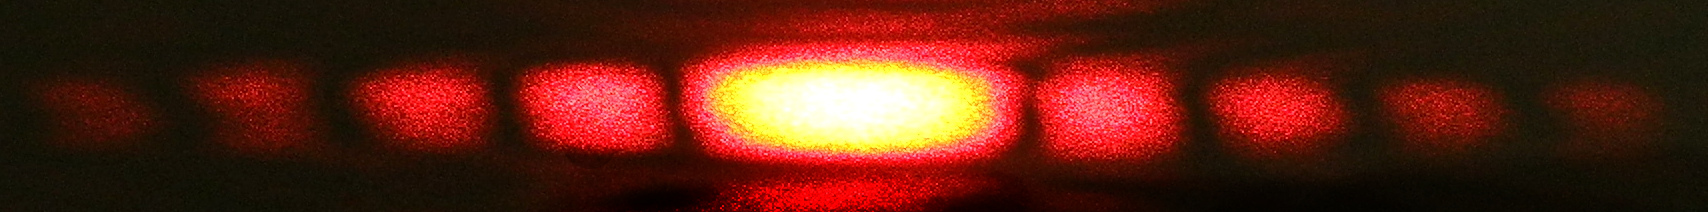
\includegraphics[width=90truemm]{slike/05_photos_Fraunhofer.jpg}
\caption{Fotografija Fraunhoferjeve uklonske slike na eni reži}
\label{fig:05_FranuhoferFoto}
\end{figure}

V smeri naprej je intenziteta uklonjene svetlobe največja, nato z naraščajočim
kotom pojema, dokler ne doseže vrednosti 0. Pri večjih kotih se pojavijo stranski
vrhovi, vendar je njihova intenziteta znatno manjša kot v osrednjem vrhu. 

Uklonske kote, pri 
katerih se pojavijo oslabitve, izračunamo preprosto iz enačbe~(\ref{eq:uklon1reza}), tako da
števec postavimo na nič. Sledi:
\beq
kd \sin \vartheta/2 = N\pi \qquad \mathrm{in} \qquad \sin \vartheta = \frac{N\lambda}{d},
\label{eq:05_24}
\eeq
pri čemer je $N$ celo število. Lego vrhov je treba določiti numerično, saj 
vrhovi ne ležijo točno na sredini med dvema oslabitvama. Povejmo še, da 
se z naraščajočo širino reže $d$ uklonski vrhovi gostijo in uklonska slika oža
(slika~\ref{fig:05_Rezad}\,a). Po drugi strani se pri zelo ozkih režah uklonski 
vrhovi razširijo in celotna uklonska slika seže globoko v območje sence 
(slika~\ref{fig:05_Rezad}\,b).
\begin{figure}[ht]
\centering
\def\svgwidth{110truemm} 
\input{slike/05_Fraunhofer_d.pdf_tex}
\caption{Shema Fraunhoferjeve uklonske slike na eni reži. 
Širša reža da razmeroma ozke vrhove in ozko
uklonsko sliko (a), ozka reža pa široke uklonske vrhove, ki sežejo globoko v območje 
geometrijske sence (b).}
\label{fig:05_Rezad}
\end{figure}
\vglue-5truemm

\end{example}

\begin{example}{\bf Fraunhoferjev uklon na pravokotni reži.}
 V prejšnjem primeru smo obravnavali enodimenzionalni primer uklona, v tem
 primeru pa integral razširimo v dve dimenziji. Ker sta integrala v izrazu
 za uklonsko sliko (enačba~\ref{eq:Fraunhoferjev}) povsem ekvivalentna, 
 lahko rezultat preprosto zapišemo. Za pravokotno režo z merama 
 $a$ v smeri $x$ in $b$ v smeri $y$ uklonsko sliko zapišemo kot:
 \beq
 j = j_0 \left(\frac{\sin\left(ka\sin \vartheta_\xi/2\right)}{ka\sin\vartheta_\xi/2}\right)^2
 \left(\frac{\sin\left(kb\sin \vartheta_\eta/2\right)}{kb\sin\vartheta_\eta/2}\right)^2\!\!,
 \eeq
 pri čemer smo izhodišče postavili na sredino odprtine. Uklonski vzorec
 je prikazan na sliki~\ref{fig:05_pravokot}.
 \begin{figure}[ht]
\centering
\centering
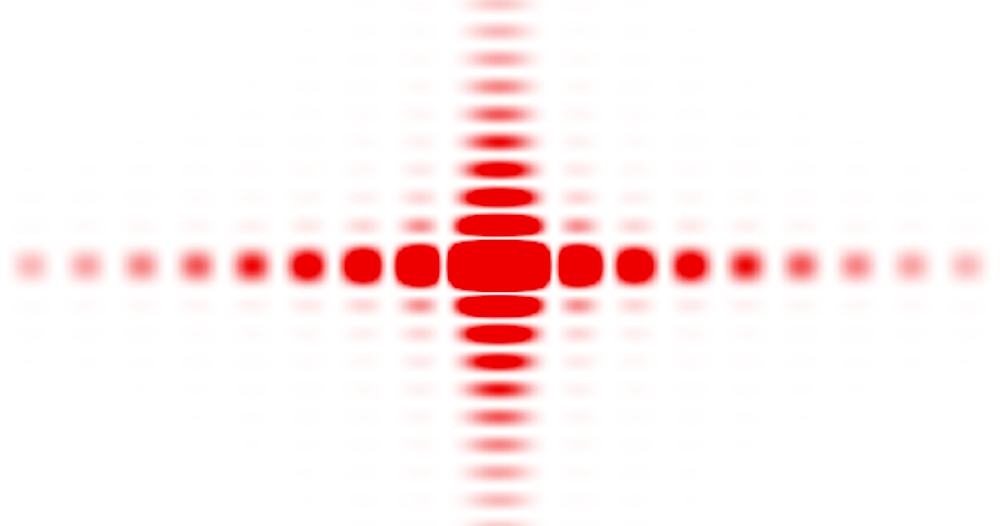
\includegraphics[width=100truemm]{slike/05_pravokot.png}
\caption{Simulacija uklonske slike na pravokotni reži
za razmerje stranic $a:b = 1:2$.}
\label{fig:05_pravokot}
\end{figure}
\vglue-5truemm

\end{example}

\begin{example}{\bf Fraunhoferjev uklon na sistemu $N$ vzporednih rež.}
Naj bo v objektni ravnini $N$ vzporednih rež debeline $d$, perioda ponavljanja
rež pa naj bo $D$. Izračunajmo uklonsko sliko, ki nastane na opazovalnem zaslonu.

Podobno kot smo izračunali uklonsko sliko na eni reži, izračunamo tudi uklonsko sliko
na več vzporedih režah. Prepustnostna funkcija $f$ je enaka 1 v vsaki reži, med
režami in zunaj območja rež pa je enaka 0. Zapišemo:
\beq
E(\omega_\xi) = K
\left( \int_{-d/2}^{d/2} e^{-i\omega_\xi x} dx + \int_{D-d/2}^{D+d/2} e^{-i\omega_\xi x} dx +
\int_{2D-d/2}^{2D+d/2} e^{-i\omega_\xi x} dx + ... \right)\!\!.
\label{eq:05_25}
\eeq
Integrale izračunamo in dobimo:
\beq
E(\omega_\xi) = \frac{K}{-i\omega_\xi}
\left(e^{-i\omega_\xi d/2}- e^{i\omega_\xi d/2} \right) \left(1 + e^{-i\omega_\xi D} + 
e^{-i\omega_\xi 2 D} + ...\right)\!.
\label{eq:05_26}
\eeq
Geometrijsko vrsto v oklepaju seštejemo, uporabimo izraz za sinus in dobimo:
\beq
E(\omega_\xi) = Kd
\frac{e^{-iN\omega_\xi D/2}} {e^{-i\omega_\xi D/2}}
\frac{\sin(\omega_\xi d/2)}{\omega_\xi d/2} 
\frac{\sin(N\omega_\xi D/2)}{\sin(\omega_\xi D/2)}.
\label{eq:05_27}
\eeq
Gostota svetlobnega toka uklonjene svetlobe na opazovalnem zaslonu je tako:
\boxeq{eq:uklonNrez}{
j(\vartheta) = j_0 \left(\frac{\sin\left(kd\sin\vartheta/2\right)}{kd\sin\vartheta/2}\right)^2
\left(\frac{\sin\left(NkD\sin\vartheta/2\right)}{\sin\left(kD\sin\vartheta/2\right)}\right)^2\!\!.
}
Prvi oklepaj imenujemo strukturni faktor $S(\vartheta)$ in določa ovojnico 
uklonske slike. Enak je uklonski sliki za eno samo režo debeline $d$ 
(enačba~\ref{eq:uklon1reza}). 
Drugi oklepaj imenujemo mrežni faktor $M(\vartheta)$ in je odvisen od števila
in razporeditve rež (glej sliko~\ref{fig:05_Nrez}). 

\begin{figure}[ht]
\centering
\def\svgwidth{140truemm} 
\input{slike/05_Fraunhofer_N.pdf_tex}
\caption{Fraunhoferjeva uklonska slika na $N$ vzporednih režah. 
Primer je narisan za $N=5$ rež in $D=3d$. Strukturni faktor $S$ (modra) je 
enak kot uklonska slika ene reže. Produkt med strukturnim faktorjem in mrežnim
faktorjem $M$ (zelena) da celotno uklonsko sliko (rdeča). Nad izračunano
uklonsko sliko je simulacija uklonske slike laserskega snopa na enaki uklonski oviri.
Parameter $x = d\sin \vartheta/\lambda$.}
\label{fig:05_Nrez}
\end{figure}

Glavne vrhove v uklonski sliki dobimo, kadar je imenovalec mrežnega faktorja enak nič in velja:
\boxeq{eq:05_28}{
kD \sin\vartheta/2 = n\pi \qquad \mathrm{in} \qquad D \sin \vartheta = n\lambda,
}
pri čemer je $n$ celo število. Med posamičnimi glavnimi vrhovi se pojavijo še manjši
stranski vrhovi. Poiščemo jih med zaporednimi minimumi, ki jih določajo ničle števca
ulomka:
\beq
NkD \sin(\vartheta)/2 = m\pi \qquad \mathrm{in} \qquad \sin \vartheta = \frac{m\lambda}{ND},
\label{eq:05_29}
\eeq
pri čemer je $m$ celo število. Med dvema glavnima vrhoma je na splošno
$N-2$ stranskih vrhov. Pri izračunu amplitude vrhov moramo upoštevati
tudi strukturni faktor, torej ovojnico.
\begin{figure}[ht]
\centering
\def\svgwidth{140truemm} 
\input{slike/05_Fraunhofer_2.pdf_tex}
\caption{Fraunhoferjeva uklonska slika na dveh vzporednih režah $N=2$ za $D=4d$. 
Produkt med strukturnim faktorjem $S$ (modra) in mrežnim
faktorjem $M$ (zelena) da celotno uklonsko sliko (rdeča). Pod simulacijo uklonske 
slike laserskega snopa je fotografija uklonske slike.}
\label{fig:05_2rezi}
\vglue-5truemm
\end{figure}

Poglejmo še limito v primeru zelo tankih rež. Strukturni faktor, ki opisuje uklon na 
eni sami reži, se močno razširi in v limiti $d\to 0$ velja $S(\vartheta) \to 1$. Envelopa
tako postane konstantna in amplituda vrhov v tem primeru ne pojema več z naraščajočim 
$\vartheta$. Uklonska slika je tako enaka mrežnemu faktorju (glej sliko~\ref{fig:05_Nrez}, modra črta).
\begin{figure}[ht]
\centering
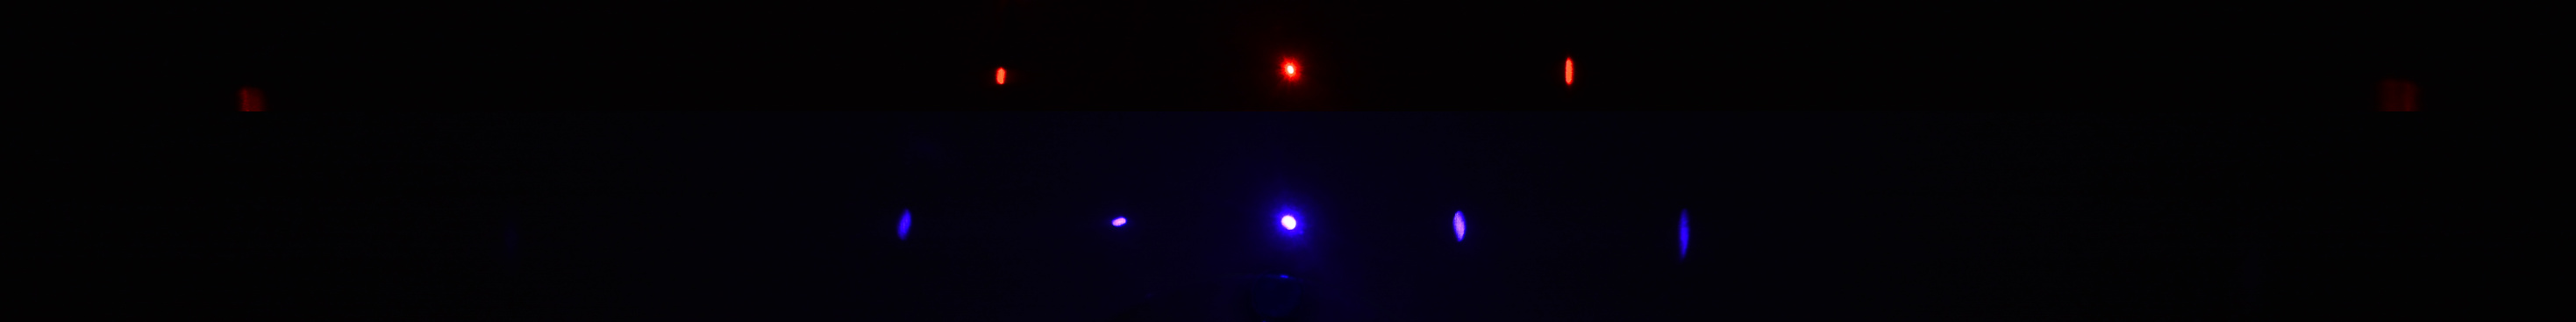
\includegraphics[width=140truemm]{slike/05_photos_CD.JPG}
\caption{Primer zelo velikega števila zelo tankih rež je zgoščenka (CD). Če z nje odstranimo
odbojno kovinsko plast, ostane prozorna plastična ploščica z vrezanim zapisom, na katerem se uklanja 
vpadna laserska svetloba. Različne valovne dolžine se uklanjajo pod različnimi koti, kar
da zgoščenkam značilen mavrični videz.}
\label{fig:05_uklon_cd}
\vglue-5truemm
\end{figure}
\begin{figure}[ht]
\centering
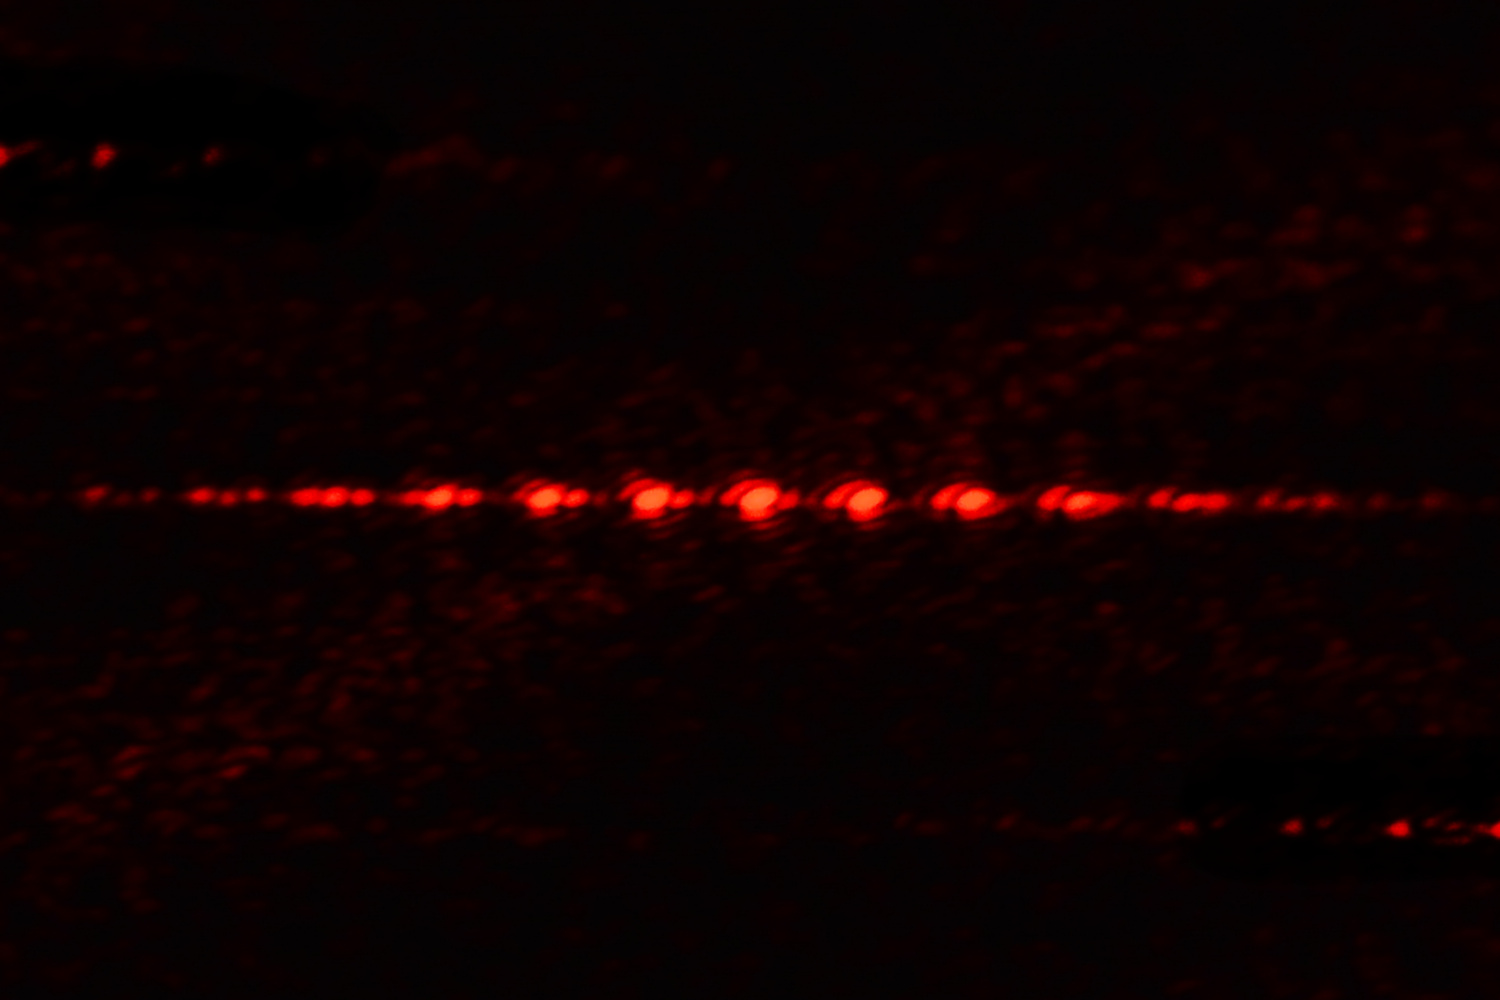
\includegraphics[width=70truemm]{slike/05_photos_perje.jpg}\hfill
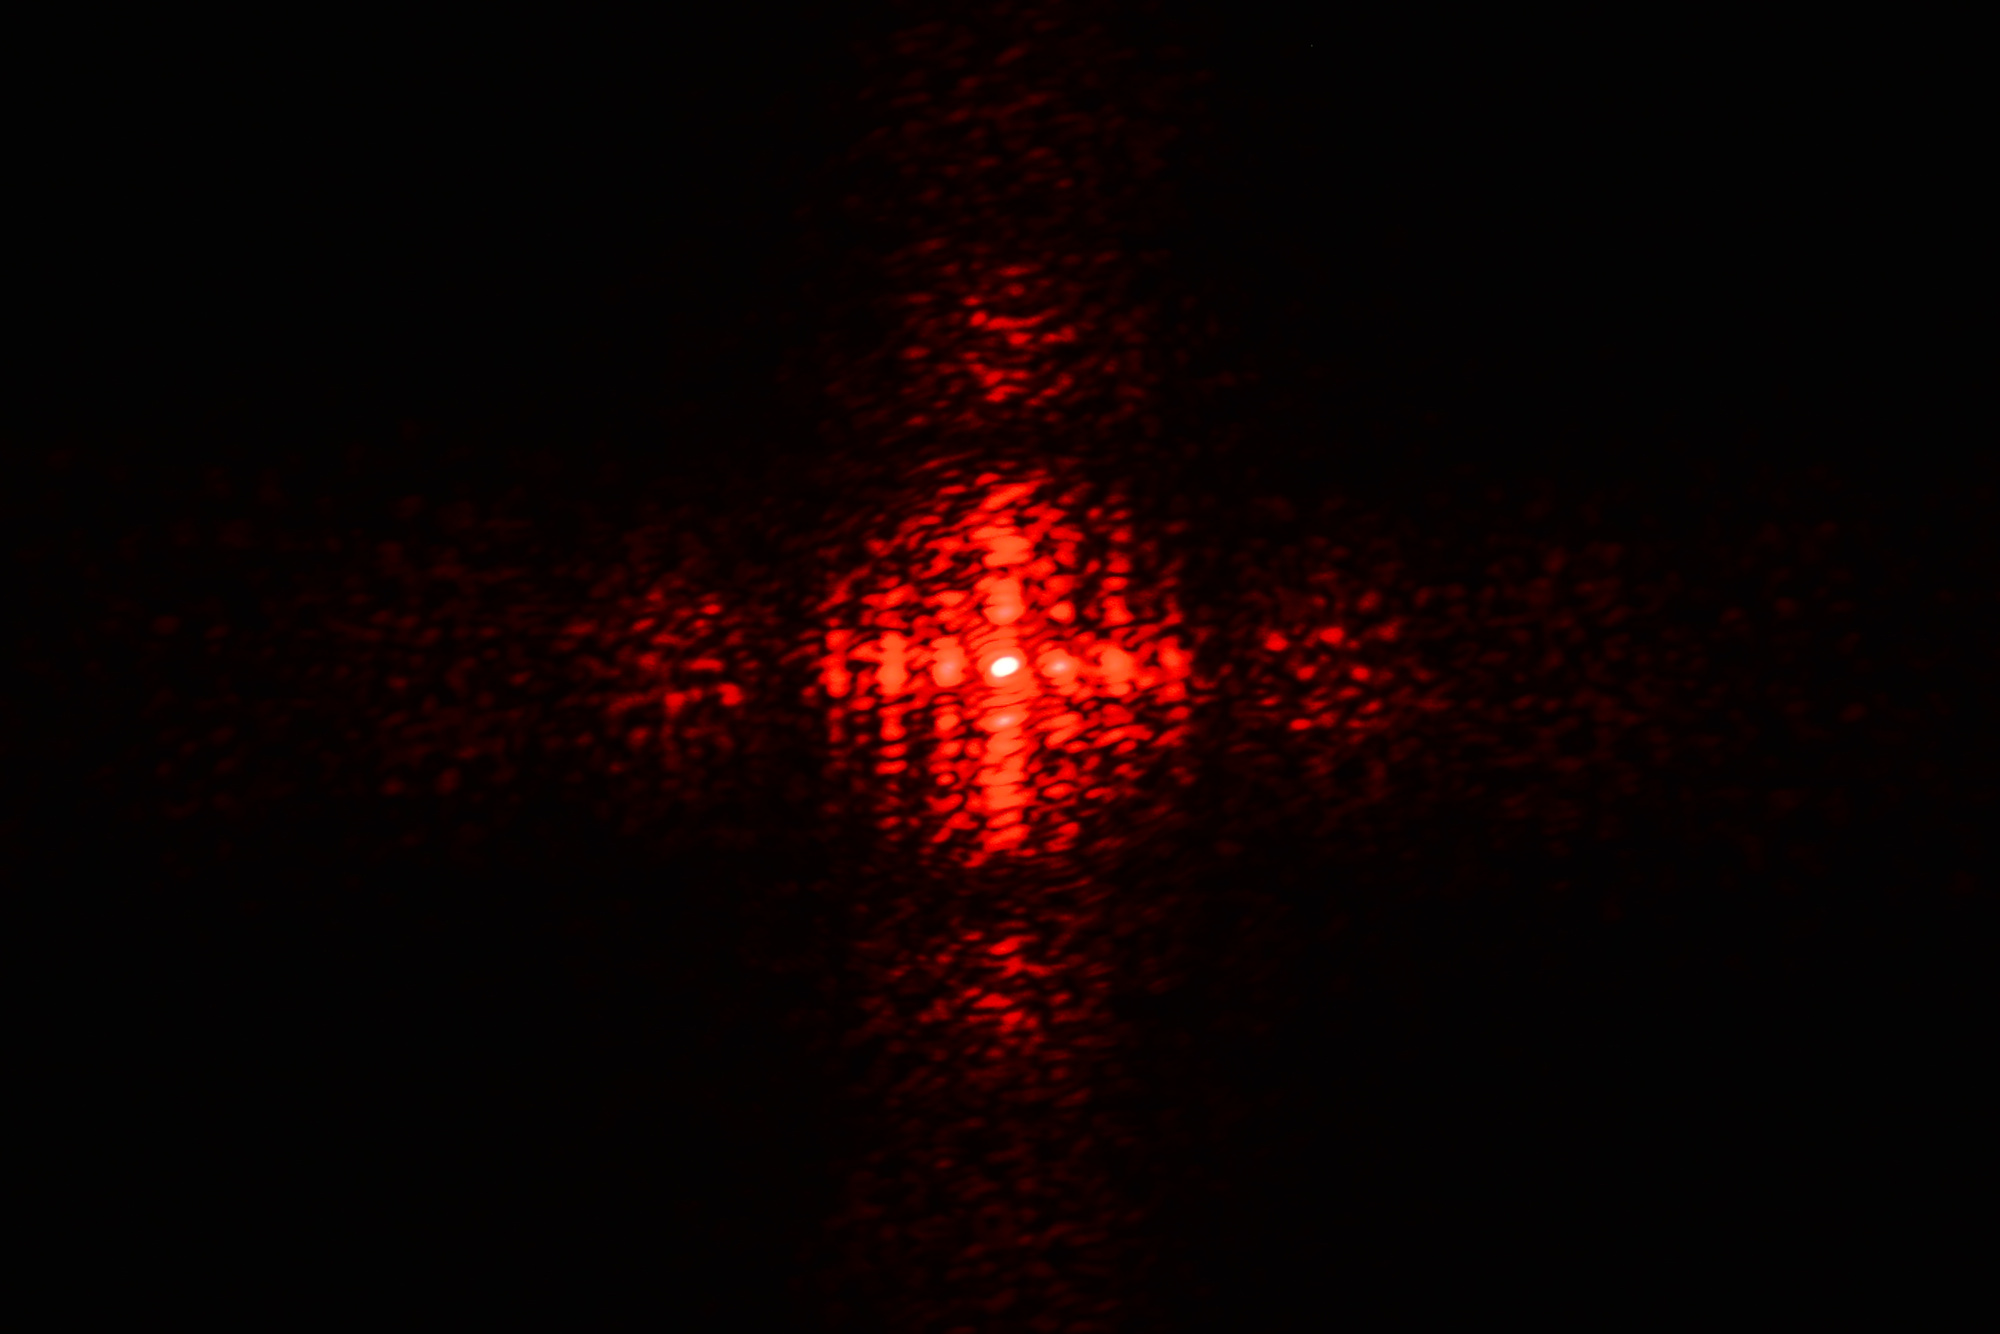
\includegraphics[width=70truemm]{slike/05_photos_ruta.jpg}
\caption{Uklon laserske svetlobe na ptičjem peresu (levo) in na gosto tkani svileni ruti (desno).
Dvodimenzionalna uklonska slika je produkt uklonskih slik v smereh $x$ in $y$.}
\label{fig:05_uklon_ruta}
\end{figure}
\vglue-5truemm
\end{example}

\begin{example}{\bf Fraunhoferjev uklon na okrogli odprtini s polmerom $a$.}
Kot naslednji primer si oglejmo Fraunhoferjev uklon na okrogli odprtini s polmerom $a$. 
Lego točke $P$ v objektni ravnini $xy$ opišemo v polarnih koordinatah $\varrho$ in $\varphi$
kot:
\beq
x = \varrho \cos \varphi \qquad \mathrm{in} \qquad y = \varrho \sin \varphi. 
\label{eq:05_30}
\eeq
Lego točke $P_0$ v opazovalni ravnini $\xi \eta$ zapišemo v polarnih koordinatah 
$q$ in $\phi$:
\beq
\xi = q \cos \phi \qquad \mathrm{in} \qquad \eta = q \sin \phi. 
\label{eq:05_31}
\eeq
\begin{figure}[ht]
\vglue-5truemm
\centering
\def\svgwidth{130truemm} 
\input{slike/05_koordinate_circ.pdf_tex}
\caption{Za izračun uklona na okrogli odprtini vpeljemo polarna koordinatna sistema 
($\varrho, \varphi$) na objektni ravnini in ($q, \phi$) na opazovalni ravnini.}
\label{fig:05_koordinate_circ}
\end{figure}

Uklonski integral (enačba~\ref{eq:Fraunhoferjev}) v novih koordinatah zapišemo kot:
\beq
E(q,\phi,z_0) = \frac{i}{\lambda} \frac{E_0e^{ikR_0}}{R_0}\int_0^{2\pi} \int_0^a
e^{-i\omega_\xi x}e^{-i\omega_\eta y}\varrho d\varrho d\varphi.
\label{eq:05_32}
\eeq
Upoštevamo enačbe~(\ref{eq:05_13}, \ref{eq:05_14}, \ref{eq:05_30} in \ref{eq:05_31}) in zapišemo:
\beq
\omega_\xi x + \omega_\eta y= \frac{k}{R_0}q\cos \phi \varrho \cos\varphi + 
\frac{k}{R_0}q\sin \phi \varrho \sin\varphi = 
 \frac{k}{R_0} q\varrho\cos(\varphi - \phi).
\label{eq:05_33}
\eeq
Zaradi rotacijske simetrije lahko postavimo $\phi=0$ in zapišemo integral:
\beq
E(q,z_0) = \frac{i}{\lambda} \frac{E_0e^{ikR_0}}{R_0}\int_0^{2\pi} \int_0^a
e^{-ikq\varrho \cos\varphi/R_0} \varrho d\varrho d\varphi.
\label{eq:05_34}
\eeq
Spomnimo se integralnega zapisa Besslove funkcije prve vrste ničtega reda:
\beq
J_0(u) = \frac{1}{2\pi} \int_0^{2\pi} e^{-iu\cos v }dv
\label{eq:05_35}
\eeq
in rekurzijske zveze:
\beq
\frac{d}{du}\left( u J_1(u)\right) = u J_{0}(u).
\label{eq:05_36}
\eeq
Primerjamo enačbi~(\ref{eq:05_34}) in (\ref{eq:05_35}) in vpeljemo
zvezi $v = \varphi$ in $u = kq\varrho/R_0$. Integriramo enačbo~(\ref{eq:05_34}) 
najprej po $\varphi$ z upoštevanjem enačbe~(\ref{eq:05_35}), nato še po $\varrho$
z upoštevanjem enačbe~(\ref{eq:05_36}). Dobimo:
\beq
E = \frac{i}{\lambda}\frac{E_0 e^{ikR_0}}{R_0}~\pi a^2~\frac{2 J_1 (kqa/R_0)}{kqa/R_0}.
\label{eq:05_37}
\eeq
Vpeljemo uklonski kot $\vartheta \approx q/R_0$ in zapišemo gostoto svetlobnega toka
uklonjene svetlobe:
\boxeq{eq:uklonAiry}{
j = j_0 \left(\frac{2J_1(ka\sin\vartheta)}{ka\sin \vartheta}\right)^2\!\!.
}
Opisano uklonsko sliko imenujemo Airyjeva uklonska slika 
in osrednji krog Airyjev disk 
po angleškem matematiku in astronomu Siru Georgeu Biddellu Airyu (1801--1892). 
Uklonska slika je  po pričakovanju rotacijsko simetrična.  
\begin{figure}[ht]
\centering
\centering
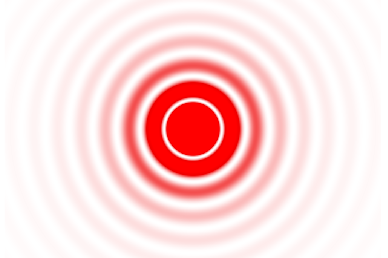
\includegraphics[width=7truecm]{slike/05_circ_sim.png}\hfill
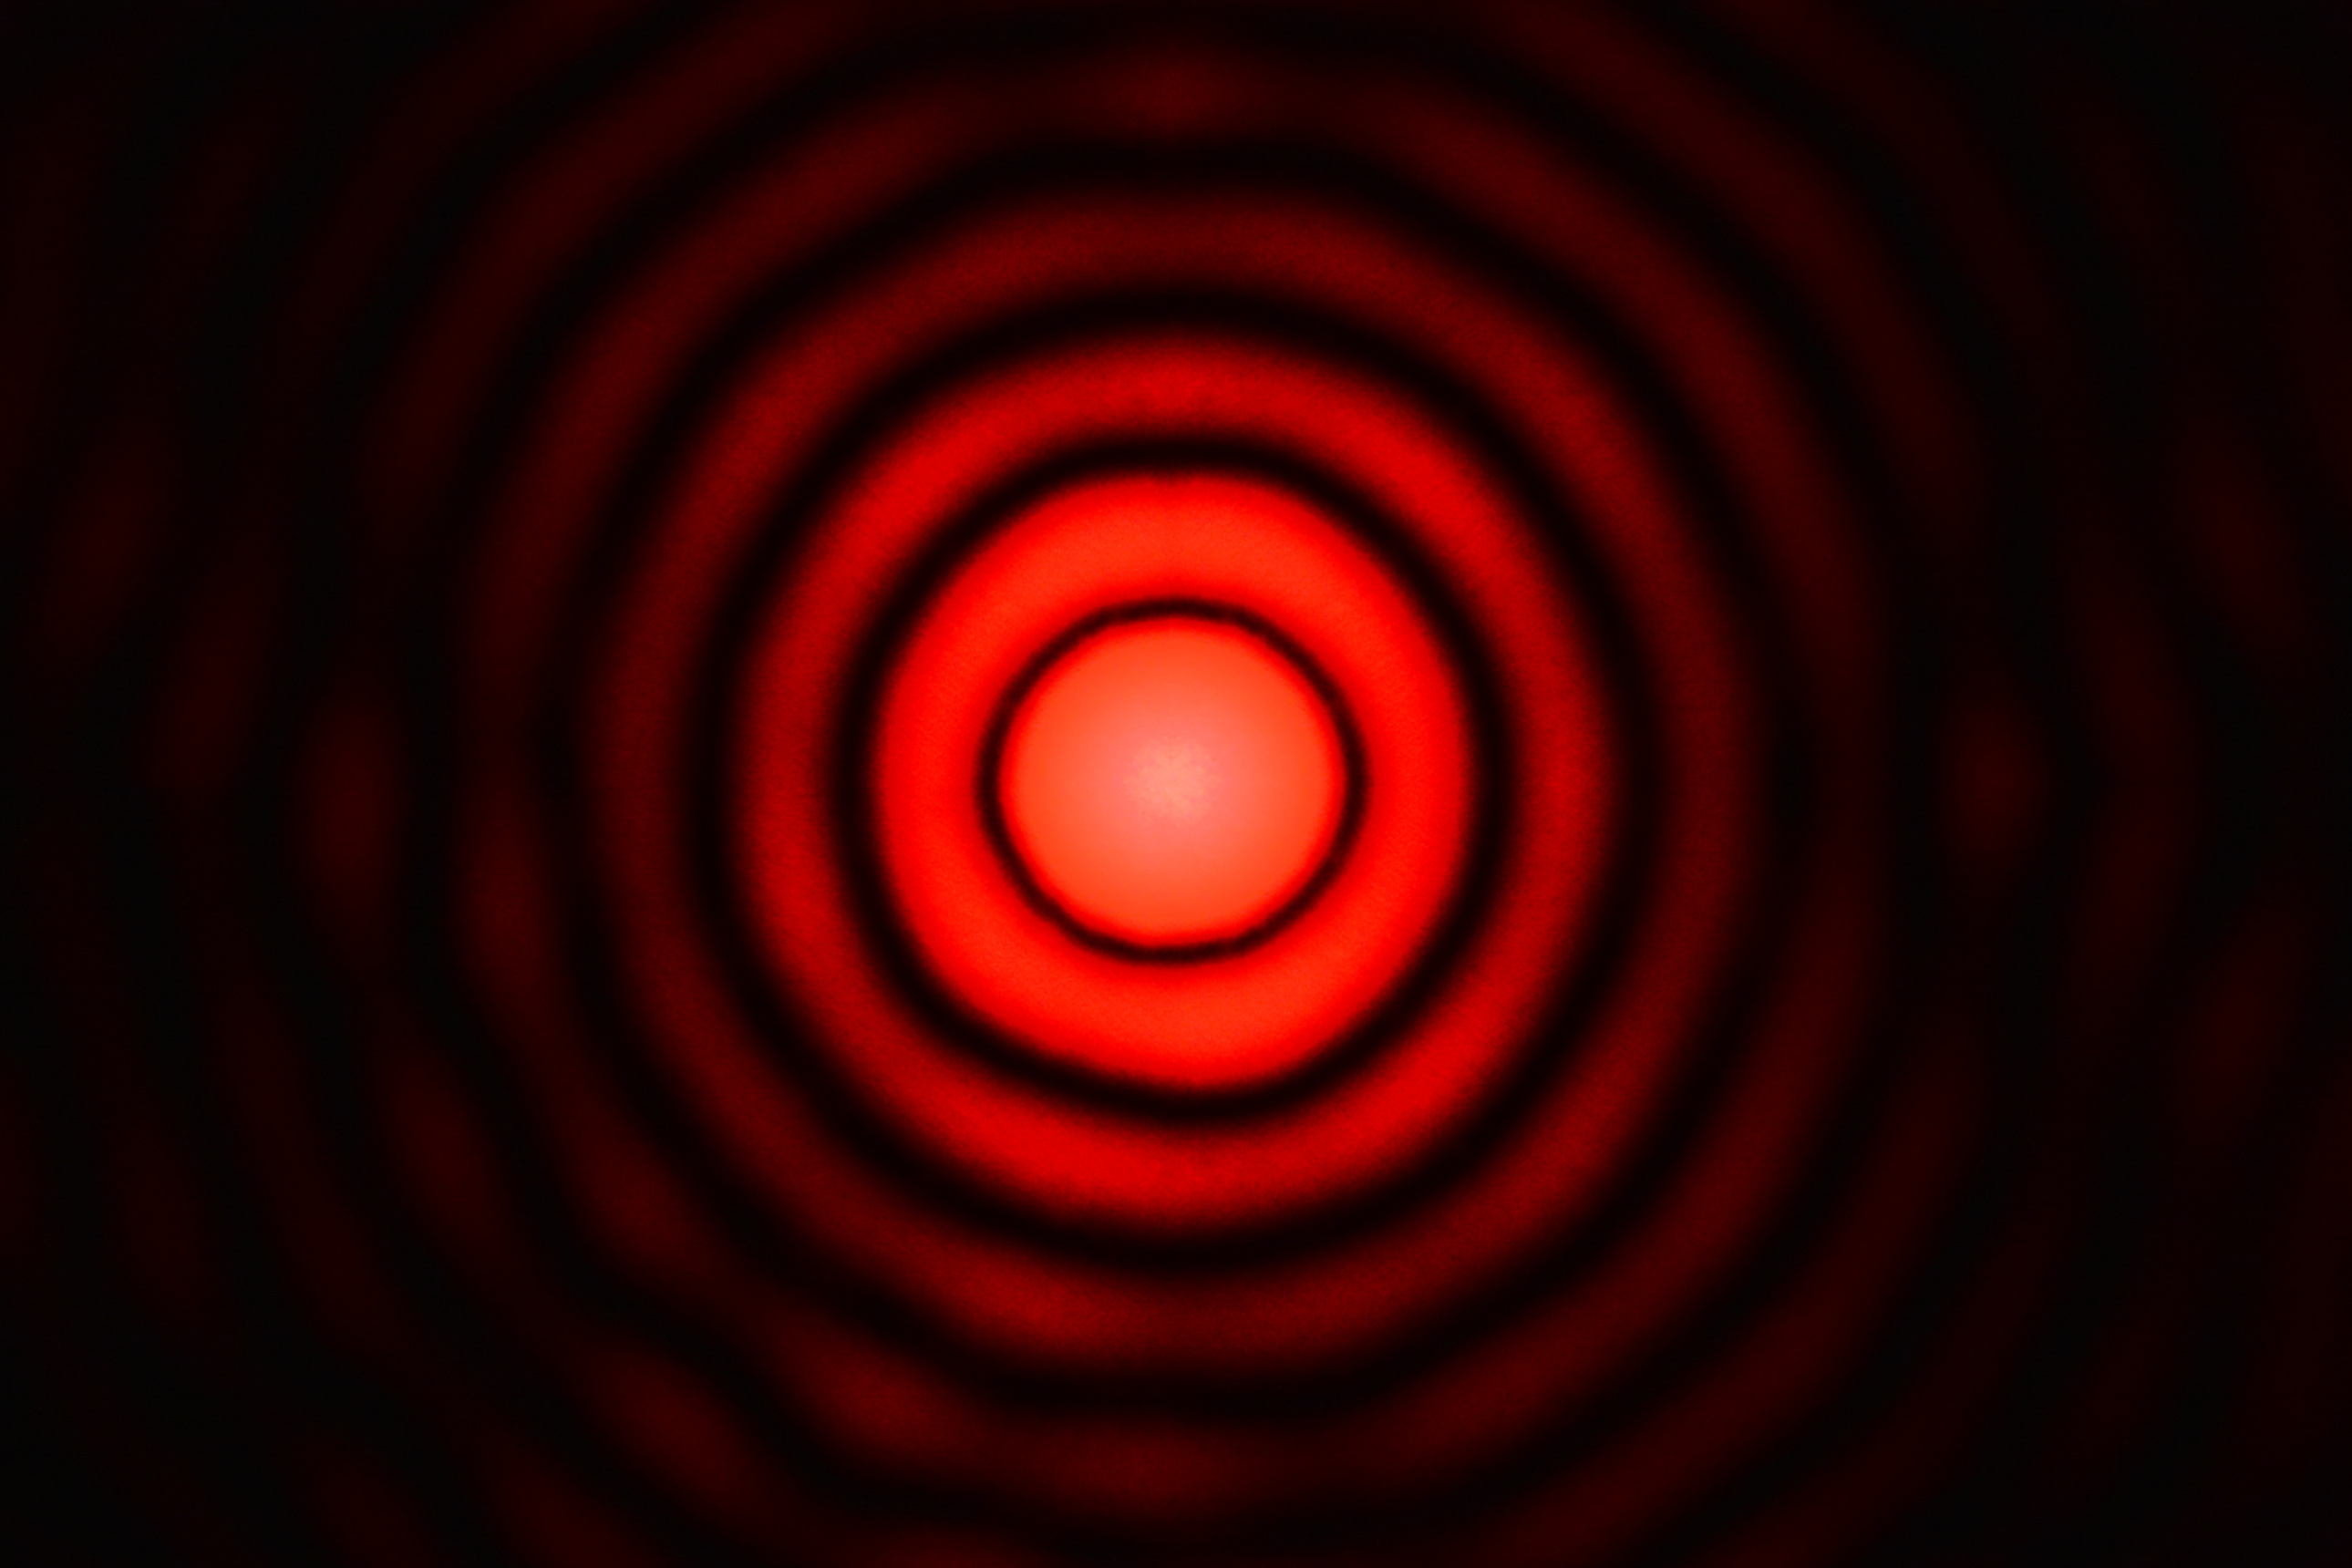
\includegraphics[width=7truecm]{slike/05_circ.JPG}
\caption{Simulacija Fraunhoferjeve uklonske slike na okrogli odprtini in fotografija
uklona na luknjici v papirju.}
\label{fig:05_Airy}
\end{figure}

V smeri naravnost (na sredini Airyjevega diska) 
je gostota svetlobnega toka enaka $j_0$, saj velja:
\beq
\lim_{u \to 0}\frac{J_1(u)}{u} = \frac{1}{2}.
\label{eq:05_39}
\eeq
Z naraščajočim uklonskim kotom intenziteta uklonjene svetlobe pojema, nato
spet naraste in ponovno pojema ... Ničle uklonske slike so določene
z ničlami Besslove funkcije in se pojavijo pri vrednostih:
\beq
ka\sin\vartheta  \approx 3,83;~7,02;~10,17;~13,32~...
\label{eq:05_40}
\eeq
Intenziteta stranskih obročev je razmeroma šibka, zato je najpomembnejši
notranji krog uklonske slike. Inteziteta prvega obroča je namreč le okoli $2~\%$ vršne
intenzitete, ostali obroči pa so še občutno šibkejši.

Polmer notranjega kroga (Airyjevega diska) $q_A$ izračunamo iz zveze:
\beq
ka\,q_A/R_0 = \frac{2\pi a}{\lambda}\frac{q_A}{R_0} = 3,83
\label{eq:05_41}
\eeq
in dobimo:
\beq
q_A = \frac{3,83}{\pi}\frac{\lambda R_0}{2a} = 1,22~\frac{\lambda R_0}{2a}.
\label{eq:05_42}
\eeq

Po Babinetovem načelu nastane enaka uklonska slika, če se svetloba uklanja
na okrogli odprtini v zaslonu ali na okroglem predmetu. Primer majhnih okroglih
predmetov, ki jih v velikem številu najdemo v naravi, so oblaki. Ko na primer svetloba
s Sonca ali z Lune vpada na plast drobnih kapljic v ozračju, se na njih uklanja in pojavi se
tako imenovana korona. Podoben pojav opazimo na zarošenem oknu. 
\begin{figure}[ht]
\centering
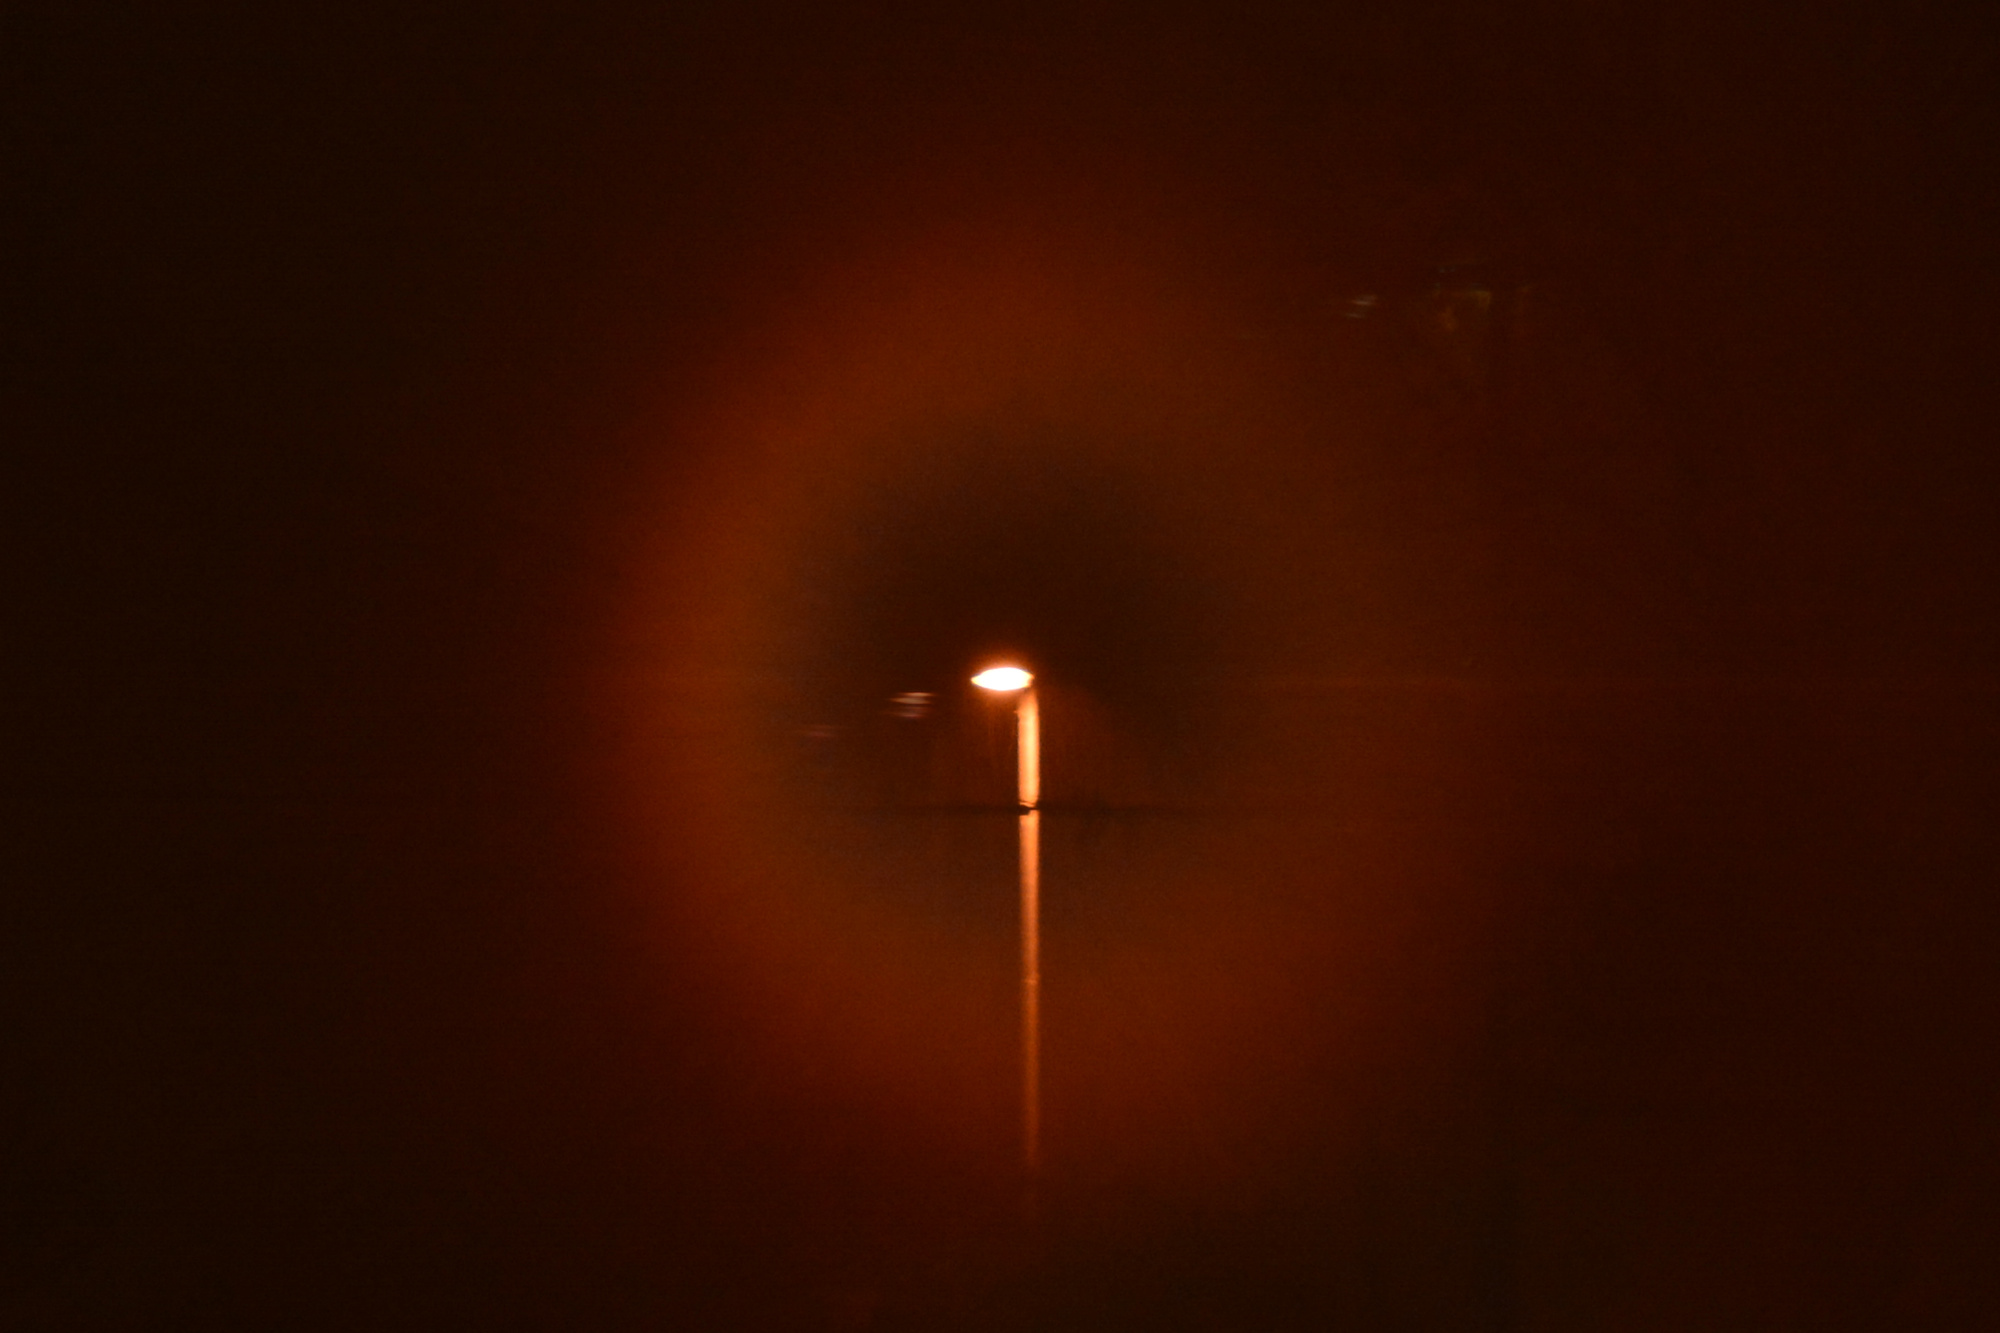
\includegraphics[width=70truemm]{slike/05_photos_svetilka.jpg}\hfill
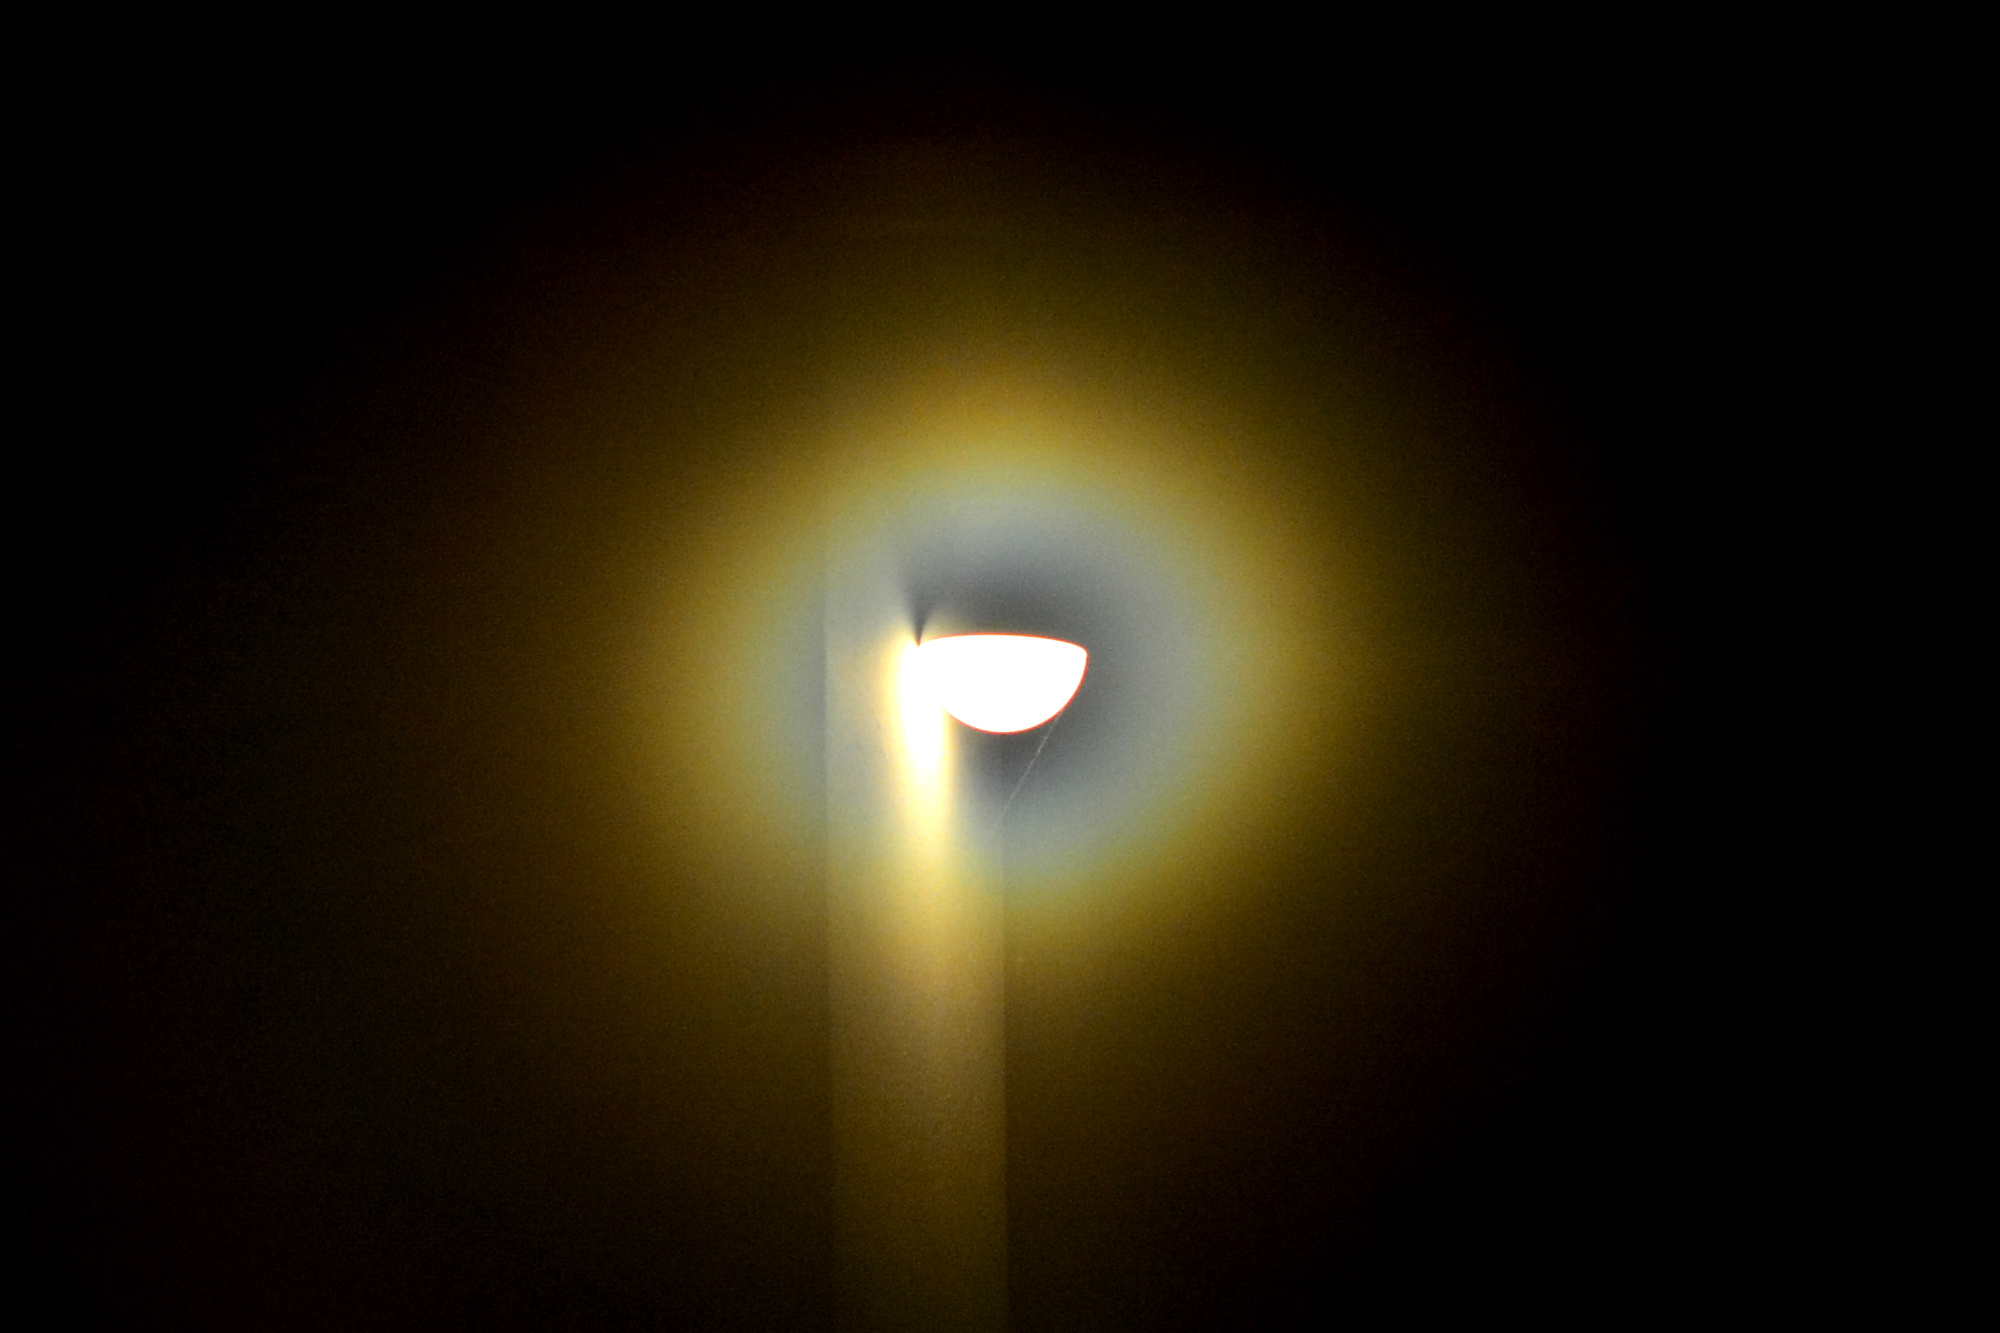
\includegraphics[width=70truemm]{slike/05_photos_luc.jpg}
\caption{Svetloba s svetilke se uklanja na drobnih kapljicah na zarošenem oknu (levo). Če je svetloba
bela, se različne barve uklanjajo pod različnimi koti in vidimo barvne obroče (desno).}
\label{fig:05_uklon_svetilka}
\end{figure}
\vglue-5truemm

\end{example}

\section{Ločljivost optičnih naprav}
Pri optičnih napravah (na primer mikroskopu ali daljnogledu) 
svetloba potuje skozi leče in nato vpade na svetlobni detektor. Leče pri tem delujejo
kot okrogle odprtine, na katerih se svetloba uklanja, kar omejuje ločljivost 
optičnih naprav.

Poglejmo najpreprostejši primer ene same leče z goriščno razdaljo $f$ in premerom $D$,
skozi katero opazujemo zelo oddaljen točkast predmet. Slika predmeta 
nastane v goriščni ravnini, zato je $R_0=f$. Zaradi uklona točkasti predmet na 
detektorju po enačbi~(\ref{eq:05_42}) vidimo kot okrogel disk s polmerom $q$:
\beq
q \approx q_A = 1,22~\frac{f\lambda}{D} = 1,22~\frac{\lambda}{D/f} = 0,61~\frac{\lambda}{NA},
\label{eq:05_43}
\eeq
pri čemer je numerična apertura $NA$ razmerje med polmerom leče $D/2$
in goriščno razdaljo $f$:
\beq
NA = \frac{D/2}{f}.
\label{eq:05_44}
\eeq
Značilne vrednosti za numerično aperturo so $NA \lesssim 1$.

Opazujmo dve oddaljeni točkasti telesi skozi lečo z numerično aperturo $NA$. 
V opazovalni ravnini vsako od njiju ustvari svoj Airyjev disk. Kadar se začneta osrednja
kroga uklonske slike med seboj prekrivati, teles na sliki ne moremo več ločiti. Kriterij, ki določa,
ali dva objekta na sliki še ločimo med seboj, imenujemo
Rayleighev kriterij ločljivosti po angleškemu fiziku Lordu Rayleighu (1842--1919). 
\begin{figure}[ht]
\centering
\def\svgwidth{120truemm} 
\input{slike/05_locljivost.pdf_tex}
\caption{Ko se uklonski sliki dveh točkastih predmetov prekrivata, ju ne moremo več ločiti.
Najmanjši kot $\alpha$, pri katerem predmeta še ločimo, določa ločljivost naprave.}
\label{fig:05_locljivost}
\end{figure}

\begin{figure}[ht]
\centering
\def\svgwidth{120truemm} 
\input{slike/05_locljivost2.pdf_tex}
\caption{Po Rayleighevem kriteriju sliki dveh teles ločimo, če je razdalja med
njunima središčema večja (levo) ali enaka polmeru Airyjevega diska (sredina). Če 
sta sliki teles bliže, ju ne ločimo (desno).}
\label{fig:05_locljivost2}
\end{figure}

Rayleighev kriterij pravi, da objekta ločimo, če velja:
\beq
\alpha \ge \alpha_{\mathrm{min}} = 
\frac{q_{A}}{f} = 1,22~\frac{\lambda}{D}.
\label{eq:05_46}
\eeq
Manjši minimalni zorni kot in s tem večjo kotno 
ločljivost optičnih naprav, na primer teleskopov, torej
dosežemo pri manjših valovnih dolžinah svetlobe in večjih lečah.

Na podoben način izračunamo tudi ločljivost optičnih mikroskopov. Ker
je pri mikroskopih predmet blizu goriščne razdalje, je najmanjši 
razmik med točkama, ki ju še ločeno opazujemo, enak:
\beq
d_\mathrm{min} = \alpha_{\mathrm{min}} f = 1,22~\frac{\lambda f}{D} = 
0,61~\frac{\lambda}{NA} \sim \lambda.
\label{eq:05_46aa}
\eeq
Ločljivost mikroskopov je tako približno enaka 
valovni dolžini svetlobe, s katero opazujemo predmet: 
$d_\mathrm{min} \sim \lambda$.

\begin{remark}
Ločljivost optičnih naprav izboljšamo z uporabo krajše valovne dolžine svetlobe.
Z modro svetlobo tako lahko opazujemo manjše predmete
kot z rdečo. Uporaba krajše valovne dolžine med drugim omogoča zgostitev 
zapisa na zgoščenkah. Z navadne zgoščenke (CD) beremo podatke z valovno 
dolžino $780~\si{\nano\metre}$, z zgoščenke DVD z valovno dolžino
$650~\si{\nano\metre}$ in z Blu-ray plošč s svetlobo z valovno dolžino
$405~\si{\nano\metre}$, kar omogoča gostejši zapis večje količine podatkov.
Dodatno se pri novejših tehnologijah uporablja lečo z večjo numerično
aperturo, kar zmanjša polmer laserske pike
z $800~\si{\nano\metre}$ na $250~\si{\nano\metre}$.
\end{remark}

\begin{example}{\bf Ločljivost teleskopa.}
S teleskopom, ki ima lečo s premerom $D=5~\si{m}$,
opazujemo Luno, ki je od Zemlje oddaljena $L = 384\,000~\si{km}$. 
Ocenimo velikost podrobnosti na Luninem površju, ki jih še ločimo
s svetlobo z valovno dolžino $500~\si{nm}$. 

Iz enačbe~(\ref{eq:05_46}) ocenimo:
\beq
d_\mathrm{min} = 1,22~\frac{\lambda}{D} L \approx 50~\si{m}.
\label{eq:05_47}
\eeq
\end{example}

\section{Fresnelov uklon}
Doslej smo predpostavili, da je optično polje, ki vpade na objektni zaslon $xy$ povsod 
konstantno in enako $E_0$. Obravnavajmo zdaj primer, ko je svetloba, 
ki vpada na objektni zaslon, funkcija kraja $E_0 = E_0(x,y)$. 

Naj izvor svetlobe $S$, ki oddaja krogelno valovanje, leži v ravnini 
$x'y'$. Razdalja med ravnino izvora svetlobe in objektno ravnino
naj bo enaka $z_0'$ (slika~\ref{fig:05_Fresnel}).
\begin{figure}[ht]
\centering
\def\svgwidth{120truemm} 
%\input{slike/05_Fresnel.pdf_tex}
\caption{SLIKA}
\label{fig:05_Fresnel}
\end{figure}
Polje v točki $P$ v objektni ravnini potem zapišemo kot 
\beq
E_0 (x,y,0) = \tilde{E}_0 \frac{e^{ikR'}}{R'}.
\label{eq:05_65}
\eeq
Uklonski integral (enačba~\ref{eq:05_05}) se potem zapiše kot:
\beq
E(\xi, \eta, z_0) = \frac{i}{\lambda} \tilde{E}_0 \int_{-\infty}^{\infty}
\int_{-\infty}^{\infty} f(x,y) E_0 \left(\frac{e^{ikR'}}{R'}\right) \left(\frac{e^{ikR}}{R}\right) dx dy.
\label{eq:05_66}
\eeq
Izraza za $R$ in $R'$ razvijemo v Taylorjevo vrsto:
\beq
R^2 = (x-\xi)^2 + (y-\eta)^2 + z_0^2 \approx 
R_0 - \frac{x\xi}{R_0} - \frac{y\eta}{R_0} + \frac{x^2+y^2}{2R_0} + ...
\label{eq:05_67}
\eeq
Pri Fraunhoferjevem uklonu smo upoštevali prve tri člene, četrtega pa smo zanemarili.
Pri Fresnelovem uklonu upoštevamo tudi četrti člen v razvoju. 

Zapišemo razdaljo $R$ malo drugače:
\beq
R^2 = z_0^2 + (x-\xi)^2+(y-\eta)^2 = z_0^2 \left(1+ \frac{(x-\xi)^2+(y-\eta)^2}{z_0^2}\right).
\label{eq:05_68}
\eeq
Vpeljemo parameter $d^2 = (x-\xi)^2+(y-\eta)^2$ in izraz razvijemo
\beq
R = z_0^2 \left(1+\frac{d^2}{z_0^2}\right) \approx z_0 + \frac{d^2}{2z_0} + ...
\label{eq:05_69}
\eeq
Členi, ki smo jih zanemarili v razvoju, so zanemarljivi, če velja
odprtine:
\beq
k\left( \frac{1}{8}\frac{d^4}{z_0^3}\right) \ll 2\pi.
\label{eq:05_70}
\eeq
Pogoj preoblikujemo v:
\beq
\frac{d^4}{z_0^4} \ll \frac{8\lambda}{z_0}.
\label{eq:05_71}
\eeq
Kadar je zapisani pogoj izpolnjen, je Fresnelov približek veljaven.

\begin{example}
Naj bo razdalja med objektnim in opazovalnim zaslonom $z_0=1~\si{m}$ in 
valovna dolžina svetlobe $500~\si{nm}$. 
Pogoj za Fresnelov približek
uklona je izpolnjen, kadar je:
\beq
\frac{d^4}{z_0^4} \ll 8\frac{500~\si{nm}}{1~\si{m}} = 4\cdot 10^{-6},
\label{eq:05_72}
\eeq
kar pomeni, da mora za veljavnost približka veljati:
\beq
d\ll z_0 \sqrt[4]{4\cdot 10^{-6}} \approx 4~\si{mm}.
\label{eq:05_73}
\eeq
Izračunajmo še Fresnelovo število (enačba~\ref{eq:05_17}):
\beq
F = \frac{d^2}{\lambda R_0} \ll \frac{16 \times 10^{-6}~\si{m}^2}{500~\si{nm} \cdot 1~\si{m}} \approx 30. 
\label{eq:05_74}
\eeq
\end{example}

Podobno kot smo razvili $R$ (enačba~\ref{eq:05_69}), razvijemo tudi $R'$:
\beq
R' \approx z_0' + \frac{1}{2}\frac{(x-x')^2+(y-y')^2}{2z_0'}.
\label{eq:05_75}
\eeq
Oba izraza vstavimo v uklonski integral (enačba~\ref{eq:05_66}) in dobimo:
\boxeq{eq:05_76}{
E(\xi, \eta, z_0) = \frac{i}{\lambda} \frac{\tilde{E}_0 e^{ikz_0'+ikz_0}}{z_0'z_0} \int
\int_{-\infty}^{\infty} f(x,y) e^{\frac{ik}{2z_0'}((x-x')^2+(y-y')^2)} e^{\frac{ik}{2z_0}((x-\xi)^2+(y-\eta)^2)}  dx dy
}
Pri tem smo člene v imenovalcu ulomka pred integralom približali z $z_0'$ in $z_0$. Zapisani izraz
Fresnelovega približka je za analitično računanje precej zahtevnejši kot Fraunhoferjev uklon. Zato bomo obravnavali
le dva primera: Fresnelove conske plošče in uklon na pravokotni reži oziroma ostrem robu.

\begin{example}{\bf Fresnelova conska plošča.}
V objektni ravnini imamo okroglo odprtino s polmerom $a$. Oz $z$ naj poteka skozi središče odprtine. 
Točkasti izvor svetlobe leži na osi $z$ v razdalji $z_0'$ pred odprtino. Zanima nas intenziteta
svetlobe na osi $z$ v razdalji $z_0$ za odprtino.
\begin{figure}[ht]
\centering
\def\svgwidth{120truemm} 
%\input{slike/05_FresCona.pdf_tex}
\caption{SLIKA}
\label{fig:05_FresCona}
\end{figure}

Izhajamo iz enačbe~\ref{eq:05_76} in vstavimo $x'=y'=0$ in $\xi = \eta = 0$. Dobimo:
\beq
E(0,0, z_0) = \frac{i}{\lambda} \frac{\tilde{E}_0 e^{ikz_0'+ikz_0}}{z_0'z_0} \int_{-\infty}^{\infty}
\int_{-\infty}^{\infty} f(x,y) e^{(ik/2z_0')(x^2+y^2)} e^{(ik/2z_0)(x^2+y^2)} dx dy
\label{eq:05_77}
\eeq
Integral računamo v cilindričnih koordinatah in vpeljemo $\varrho = \sqrt{x^2 + y^2}$ ter
\beq
dx dy = 2 \pi \varrho d\varrho.
\label{eq:05_78}
\eeq
Funkcija $f=1$ za $\varrho \leq a$, sicer je enaka 0. Dobimo:
\beq
E(0,0, z_0) = \frac{2\pi i}{\lambda} \frac{\tilde{E}_0 e^{ikz_0'+ikz_0}}{z_0'z_0} \int_{0}^{a}
e^{\frac{ik\varrho^2}{2}\left(\frac{1}{z_0'}+\frac{1}{z_0}\right)}\varrho d\varrho.
\label{eq:05_79}
\eeq
Vpeljemo:
\beq
\frac{1}{L} = \frac{1}{z_0'} + \frac{1}{z_0} \qquad \mathrm{in} \qquad z_0'z_0 = L(z_0'+z_0).
\label{eq:05_80}
\eeq
Izračunamo integral:
\beq
\int_0^a e^{ik\varrho^2/2L}\varrho d\varrho = \frac{L}{ik}\left(e^{ika^2/2L}-1\right) = 
\frac{2L}{k}e^{ika^2/4L} \sin\left(\frac{ka^2}{4L}\right).
\label{eq:05_81}
\eeq
Za gostoto energijskega toka $j$ dobimo:
\beq
j = 4 j_0 \sin\left(\frac{ka^2}{4L}\right),
\label{eq:05_82}
\eeq
pri čemer smo z $j_0$ označili gostoto toka, kakršna bi bila na mestu opazovanja, 
če ne bi bilo zaslona:
\beq
j_0 = \frac{\tilde{E}_0^2}{(z_0'+z_0)^2}.
\label{eq:05_83}
\eeq
\begin{figure}[ht]
\centering
\def\svgwidth{120truemm} 
%\input{slike/05_FresCona2.pdf_tex}
\caption{SLIKA}
\label{fig:05_FresCona2}
\end{figure}
Na sliki~\ref{fig:05_FresCona2} je narisana odvisnost gostote svetlobnega toka na danem 
mestu od polmera odprtine $a$. Vidimo, da je največja vrednost, ki jo doseže $j$
štirikratnik intenzitete $j_0$, ki bi bila na mestu mestu opazovanja brez zaslona. 
Polmer $a_1$, pri katerem doseže vrednost $j$ prvi maksimum, imenujemo polmer
prve Fresnelove cone in je enak:
\beq
\frac{ka_1^2}{4L} = \frac{\pi}{2} \qquad \mathrm{in} \qquad a_1  = \sqrt{\lambda L}.
\label{eq:05_84}
\eeq
Prva Fresnelova cona svetlobo svetlobo torej zbira in deluje kot zbiralna leča. 
Sekundarni krogelni valovi, ki izhajajo iz območja znotraj prve Fresnelove cone, 
se seštevajo. Poglejmo račun za primer odprtine v velikosti prve Fresnelove
cone in $z_0' \to \infty$ oziroma $L = z_0$. 
\begin{figure}[ht]
\centering
\def\svgwidth{120truemm} 
%\input{slike/05_FresCona3.pdf_tex}
\caption{SLIKA}
\label{fig:05_FresCona3}
\end{figure}

Potem velja:
\beq
R^2 = z_0^2 + a_1^2 = z_0^2 + \lambda z_0.
\label{eq:05_85}
\eeq
Fazni zamik za žarek oziroma valovanje, ki izvira iz roba cone, je:
\beq
\phi_1 = kR = k\sqrt{z_0^2+\lambda z_0}.
\label{eq:05_86}
\eeq
Fazni zamik za valovanje iz sredine cone pa je:
\beq
\phi_0 = kz_0.
\label{eq:05_87}
\eeq
Dokler je fazna zakasnitev med žarki iz sredine in žarki z roba odprtine
manjša od $\pi$ oziroma razlika v dolžini poti manjša od $\lambda/2$, 
se žarki seštevajo in intenziteta na mestu $z_0$ narašča. Preverimo, ali 
se ta ugotovitev ujema s pogojem za prvo Fresnelovo cono:
\beq
R - z = \sqrt{z_0^2 + \lambda z_0} - z_0  \approx z_0 + \frac{\lambda}{2} - z_0 = \frac{\lambda}{2}.
\label{eq:05_88}
\eeq
Če polmer odprtine povečamo na območje $a>a_1$, se pojavijo valovi v protifazi in 
prispevki iz sredine odprtine in z roba odprtine se odštevajo. Zato z naraščajočim
polmerom intenziteta svetlobe pojema. Minimum doseže pri $a_2$, za katerega velja:
\beq
\frac{ka_2^2}{4L} = \pi
\label{eq:05_89}
\eeq
in $a_2 = \sqrt{2\lambda L}$. Kolobar z notranjim polmerom 
$a_1 = \sqrt{\lambda L}$ in zunanjim polmerom $a_2 = \sqrt{2\lambda L}$
imenujemo druga Fresnelova cona. Na splošno je N-ta Fresnelova cona
kolobar, ki ga omejujeta polmera $a_{N-1}$ in $a_N$:
\beq
a_{N-1} = \sqrt{(N-1)\lambda L} < a < a_{N} = \sqrt{N \lambda L}.
\label{eq:05_90}
\eeq
V tretji Fresnelovi coni $j$ spet narašča, nato v območju $a_3 - a_4$ spet pojema ...

{\bf Fresnelova uklonska leča}: Če ohranimo v ravnini $xy$ le tiste kolobarje oziroma
cone, ki so ali samo lihe ali samo sode, se prispevki vseh con seštevajo. Taka
naprava (conska plošča) zbira svetlobo na podoben način kot klasična leča. Gostota 
svetlobnega toka v točki $P_0$ je pri uporabi conske plošče dosti večja, kot bi bila 
v primeru, če bi izvor svetlobe točko osvetljeval neposredno. Tovrstne plošče so
uporabne za zabiranje svetlobe, kadar nimamo možnosti izdelave leč (na primer 
leče za žarke X. Glavna slabost Fresnelovih uklonskih leč je njihova kromatična
aberacija -- odvisnost goriščne razdalje od valovne dolžine svetlobe $f= f(L)$.
Goriščno razdaljo lahko izračunamo, da upoštevamo $z_0'\to \infty$:
\beq
\frac{1}{z_0'}+ \frac{1}{z_0}= \frac{1}{z_0} = \frac{1}{L} = \frac{1}{f},
\label{eq:05_91}
\eeq
od koder sledi:
\beq
f = \frac{a_1^2}{\lambda}.
\label{eq:05_92}
\eeq
Goriščno razdaljo conske leče z velikim številom plošč lahko tudi izračunamo:
\beq
a_{N+1}^2 - a_N^2 = \lambda (N+1)L - \lambda NL = \lambda L. 
\label{eq:05_93}
\eeq
Po drugi strani velja:
\beq
a_{N+1}^2 - a_N^2 = \left(a_{N+1}+a_N\right)\left(a_{N+1}- a_N\right) = 2\overline{a}\Delta a.
\label{eq:05_94}
\eeq
Od tod sledi:
\beq
f = \frac{a_1^2}{\lambda} = \frac{2 \overline{a}\Delta a}{\lambda}.
\label{eq:05_95}
\eeq
\end{example}

\begin{example}{\bf Fresnelov uklon na robu in pravokotni reži.}
Kot drugi primer uporabe Fresnelovega uklonskega približka 
izračunajmo uklonsko sliko na ostrem robu oziroma na pravokotni 
reži. Oz $z$ izberemo tako, da točkasti izvor svetlobe $S$ in
opazovalna točka $P_0$  ležita na njej, pravokotna reža s
koordinatami $x_1<x<x_2$ in $y_1<y<y_2$ pa naj leži v objektni
ravniki, ki je pravokotna na zveznico med točkama $S$ in $P_0$.
\begin{figure}[ht]
\centering
\def\svgwidth{120truemm} 
%\input{slike/05_FresPravokot.pdf_tex}
\caption{SLIKA}
\label{fig:05_FresPravokot}
\end{figure}

Uklonski integral (enačba~\ref{eq:05_76}) je potem:
\beq
E(0,0, z_0) = \frac{i}{\lambda} \frac{\tilde{E}_0 e^{ikz_0'+ikz_0}}{z_0'z_0} \int_{x_1}^{x_2}
\int_{y_1}^{y_2} e^{\frac{ik(x^2+y^2)}{2L}}  dx dy
\label{eq:05_96}
\eeq
oziroma:
\beq
E(P_0) \propto \int_{u_1}^{u_2} e^{i\frac{\pi}{2}u^2} du
\int_{v_1}^{v_2} e^{i\frac{\pi}{2}v^2} dv,
\label{eq:05_97}
\eeq
 pri čemer smo uvedli novi spremenljivki:
 \beq
 u = \sqrt{\frac{k}{\pi L}}x \qquad \mathrm{in} \qquad v = \sqrt{\frac{k}{\pi L}}y.
 \label{eq:05_98}
 \eeq
 Zapisana integrala izrazimo s Fresnelovima integraloma $S(x)$ in $C(x)$.
\begin{remark}
Fresnelova integrala sta oblike:
\beq
C(u) = \int_0^u \cos\left(\frac{1}{2}\pi x^2\right) dx \qquad \mathrm{in} \qquad 
S(v) = \int_0^v \sin\left(\frac{1}{2}\pi x^2\right) dx. 
\label{eq:05_99}
\eeq
\begin{figure}[ht]
\centering
\def\svgwidth{120truemm} 
%\input{slike/05_CS.pdf_tex}
\caption{SLIKA}
\label{fig:05_CS}
\end{figure}
To sta dve transcedentni funkciji, ki ju moramo izračunati numerično. Tipične
vrednosti so $C(-\infty) = -1/2$; $C(0) = 0$; $C(\infty) = 1/2$ in enako za $S$, 
pri čemer sta obe funkciji lihi. Skupaj ju združimo v integral:
\beq
\int_{0}^{u} e^{i\frac{\pi}{2}u^2} du = C(u)+iS(u) = \frac{1+i}{2}\erf \left(\frac{\sqrt{\pi}(1-i)u}{2}\right).
\label{eq:05_100}
\eeq
\end{remark}

Fresnelovo uklonsko sliko na pravokotni odprtini torej zapišemo kot:
\beq
E(P_0) \propto \left( C(u) + iS(u) \right) \left|_{u_1}^{u_2} \cdot 
\left( C(v) + iS(v) \right) \right|_{v_1}^{v_2}.
\label{eq:05_101}
\eeq

Na osnovi rezultata lahko obravnavamo tudi uklon na ravnem robu. 
To ustreza enodimenzionalnemu primeru $x_1 \to \infty$ oziroma $u_1 \to \infty$
in $x_2 = d$ oziroma $u_2  = d\sqrt{k/\pi L}$. Uklonska slika
je potem:
\beq
E(P_0) \propto C(u_2) + i S(u_2) + \frac{1}{2} + i \frac{1}{2},
\label{eq:05_102}
\eeq
od koder sledi:
\beq
j(P_0) \propto |E(P_0)|^2  \propto \left(C(u_2) + \frac{1}{2}\right)^2 + \left(S(u_2) + \frac{1}{2}\right)^2.
\label{eq:05_103}
\eeq
Zanima nas odvinost $j(d)$. Namesto da pri izračunu zaslon miruje in spreminjamo opazovalno
točko $P_0$ vzdolž osi $\xi$, točko $P_0$ ohranjamo in si mislimo, da se premika rob zaslona 
v smeri osi $x$, pri čemer negativne vrednosti $d$ ustrezajo geometrijski senci. 
\begin{figure}[ht]
\centering
\def\svgwidth{120truemm} 
%\input{slike/05_FresRob.pdf_tex}
\caption{SLIKA}
\label{fig:05_FresRob}
\end{figure}

\begin{remark}
Fresnelova integrala $C(u)$ in $S(u)$  lahko prikažemo grafično tako, da narišemo
krivuljo v parametrični obliki $C(t), S(t)$ v 2D-ravnini. 
\begin{figure}[ht]
\centering
\def\svgwidth{120truemm} 
%\input{slike/05_Cornu.pdf_tex}
\caption{SLIKA}
\label{fig:05_Cornu}
\end{figure}
Poglejmo nekaj lasnosti te parametrične krivulje, ki jo imenujemo tudi Cornujeva oziroma
Eulerjeva spirala. Pri vrednosti $t\to \infty$ je vrednost $(1/2, 1/2)$ in pri 
$t\to -\infty$ je vrednost $(-1/2, -1/2)$. 
Dolžina krivulje? Strmina krivulje? Ukrivljenost krivulje je sorazmerna z dolžino
trajektorije (poti). 
\end{remark}
\end{example}


\section{*Izpeljava Kirchhoffovega uklonskega integrala}
\label{chap:Kirchhoff}
Poglejmo še matematično izpeljavo uklonskega integrala (enačba~\ref{eq:05_01})
in najprej ponovimo Greenov teorem, ki izhaja iz Gaussovega stavka. Naj bo 
$\mathbf{W}(\mathbf{r})$ poljubno zvezno in zvezno odvedljivo vektorsko
polje. Gaussov stavek pravi, da je intergal po sklenjeni ploskvi enak
integralu divergence vektorskega polja po prostoru:
\beq
\oint_S \mathbf{W} d\mathbf{S} = \int_V \div(\mathbf{W})dV.
\label{eq:05_48}
\eeq
Zapišimo  vektorsko polje $\mathbf{W}$ s skalarnima poljema $\Psi$ in $\Phi$
v obliki:
\beq
\mathbf{W}(\mathbf{r}) = \Psi \nabla \Phi - \Phi \nabla \Psi,
\label{eq:05_49}
\eeq
pri čemer sta funkciji $\Psi$ in $\Phi$ zvezni in dvakrat zvezno odvedljivi.
Potem velja:
\beq
\div \mathbf{W}= \Psi \nabla^2 \Phi - \Phi \nabla^2 \Psi
\label{eq:05_50}
\eeq
in dobimo Greenov teorem:
\beq
\oint_S \left(\Psi \nabla \Phi - \Phi \nabla \Psi\right) d\mathbf{S}  =
\int_V \left( \Psi \nabla^2 \Phi - \Phi \nabla^2 \Psi \right) dV.
\label{eq:05_51}
\eeq
Za $\Psi$ in $\Phi$ izberemo funkciji, ki predstavljata skalarni rešitvi
krajevnega dela valovne enačbe. Za ti dve funkciji torej veljata zvezi:
\beq
\nabla^2 \Psi + k^2 \Psi = 0 \qquad \mathrm{in} \qquad \nabla^2 \Phi + k^2 \Phi = 0.
\label{eq:05_52}
\eeq
Z upoštevanjem teh dveh vez postane desni del Greenovega teorema 
(enačba~\ref{eq:05_51}) identično enak nič. Od tod sledi, da za funkciji $\Phi$ in $\Phi$,
ki sta rešitvi valovne enačbe, velja zveza:
\beq
\oint \left( \Psi\frac{\partial \Phi}{\partial \mathbf{n}} -
\Phi\frac{\partial \Psi}{\partial \mathbf{n}} \right) dS = 0.
\label{eq:05_53}
\eeq

Zamislimo si zdaj, da funkcija $\Psi$ opisuje sferične valove, ki
izhajajo iz izhodišča koordinatnega sistema $P_0$ in jo zapišemo kot:
\beq
\Psi = \frac{e^{ikr}}{r}.
\label{eq:05_54}
\eeq
Ker ta funkcija v izhodišču pri $r=0$ divergira, moramo izhodišče
izvzeti iz računa. Zato si okoli izhodišča zamislimo kroglo s 
polmerom $\varepsilon$ (slika~\ref{fig:05_Green}).
\begin{figure}[ht]
\centering
\def\svgwidth{120truemm} 
%\input{slike/05_Green.pdf_tex}
\caption{SLIKA}
\label{fig:05_Green}
\end{figure}
Celotna integracijska površina je tako sestavljena iz zunanje ploskve
$S$ in notranje krogle $S_\varepsilon$. Enačbo~(\ref{eq:05_53}) prepišemo v:
\beq
\oint_S \left( \frac{e^{ikr}}{r}\frac{\partial \Phi}{\partial \mathbf{n}} -
\Phi\frac{\partial}{\partial \mathbf{n}}\left( \frac{e^{ikr}}{r} \right) \right) dS -
\oint_{S\varepsilon} \left( \frac{e^{ikr}}{r}\frac{\partial \Phi}{\partial \mathbf{n}} -
\Phi\frac{\partial}{\partial \mathbf{n}}\left( \frac{e^{ikr}}{r} \right) \right)r^2 d\Omega = 0.
\label{eq:05_55}
\eeq
Ker je notranja ploskev krogla, je smer normale na ploskev $\mathbf{n}$ enaka smeri $\mathbf{r}$.
Potem zapišemo odvod:
\beq
\frac{\partial}{\partial r}\left( \frac{e^{ikr}}{r}\right)  = ik \frac{e^{ikr}}{r} - \frac{e^{ikr}}{r^2}.
\label{eq:05_56}
\eeq
Drugi člen v enačbi~(\ref{eq:05_55}) potem prepišemo v:
\beq
\oint_{S\varepsilon} \left( \frac{e^{ikr}}{r}\frac{\partial \Phi}{\partial \mathbf{n}}r^2 -
ik\frac{e^{ikr}}{r}r^2\Phi + \frac{e^{ikr}}{r^2}\Phi r^2 \right) d\Omega.
\label{eq:05_57}
\eeq
V limiti $\varepsilon \to 0$ gresta tako prvi kot 
drugi člen proti 0, tretji člen pa gre proti vrednosti $4\pi \Phi(P_0)$. Faktor $4\pi$ 
dobimo pri integraciji po polnem kotu. Rezultat povežemo in dobimo:
\beq
\Phi(P_0) = \frac{1}{4\pi} \oint_S \left( \frac{e^{ikr}}{r}\frac{\partial \Phi}{\partial \mathbf{n}} -
\Phi\frac{\partial}{\partial \mathbf{n}}\left( \frac{e^{ikr}}{r} \right) \right) dS.
\label{eq:05_58}
\eeq
Na ta način smo polje v opazovani točki $P_0$ izrazili s skalarnim poljem na sklenjeni površini
$S$, ki to točko obdaja.

Zdaj si zamislimo izvor valovanja $S$, ki oddaja krogelne valove oblike $\Phi = \exp(ikr')/r'$. Ti valovi
vpadajo na objektni zaslon z odprtino (slika~\ref{fig:05_Kirchhoff}), nato pa jih opazujemo 
v točki $P$ na drugi strani zaslona. Za izračun polja v točki $P$ moramo tako poznati polje na neki
sklenjeni ploskvi, ki to točko obdaja.
\begin{figure}[ht]
\centering
\def\svgwidth{120truemm} 
%\input{slike/05_Kirchhoff.pdf_tex}
\caption{SLIKA}
\label{fig:05_Kirchhoff}
\end{figure}

Integracijsko ploskev okoli točke $P$ izberemo tako, da delno poteka po zaslonu, povsod drugje
pa tako daleč stran, da so prispevki polja $\Phi$ zanemarljivo majhni. Polje na zaslonu in njegov odvod
naj bosta povsod, razen v odprtini, enaka nič. Privzamemo tudi, da je polje
v odprtini tako, kot da bi zaslona ne bilo. Potem za izračun polja v točki $P$ zadošča izračunati
integral le po površini odprtine. 

Izračunajmo smerni odvod:
\beq
\frac{\partial \Phi}{\partial \mathbf{n}} = (\nabla \Phi)\cdot \mathbf{n} = 
\frac{\partial \Phi}{\partial r'} \frac{\mathbf{r'}}{r'}\cdot \mathbf{n} = \frac{\partial \Phi}{\partial r'} 
\cos\left(\mathbf{r'},\mathbf{n}\right).
\label{eq:05_59}
\eeq
Vstavimo še funkcijo $\Phi$ in izračunamo:
\beq
\frac{\partial \Phi}{\partial r'} = \frac{\partial}{\partial r'}\left(\frac{e^{ikr'}}{r'}\right) = 
\frac{ikr'-1}{r'^2}e^{ikr'} \approx \frac{ikr'}{r'}e^{ikr'}.
\label{eq:05_60}
\eeq
Privzeli smo, da je razdalja $r'$ bistveno večja od valovne dolžine svetlobe, in 1 v števcu zanemarilli. 
Podobno izračunamo tudi drugi člen v enačbi~(\ref{eq:05_58}) in upoštevamo, da je $\lambda \ll r$. 
Uporabimo enačbi~(\ref{eq:05_59} in \ref{eq:05_60}) in ju vstavimo v enačbo~(\ref{eq:05_58}). Dobimo:
\beq
\Phi(P_0) = \frac{1}{4\pi} \int_S \left( \frac{e^{ikr}}{r} \frac{ik}{r'}e^{ikr'} \cos\left(\mathbf{r'},\mathbf{n}\right)-
\frac{e^{ikr'}}{r'} \frac{ik}{r}e^{ikr} \cos\left(\mathbf{r},\mathbf{n}\right)  \right) dS,
\label{eq:05_61}
\eeq
od koder sledi:
\beq
\Phi(P_0) = \frac{ik}{4\pi} \int_S \frac{e^{ikr}e^{ikr'}}{rr'}
\left( \cos\left(\mathbf{r'},\mathbf{n}\right) - \cos\left(\mathbf{r},\mathbf{n}\right) \right) dS.
\label{eq:05_62}
\eeq
Razliko kosinusov imenujemo tudi oblikovni faktor. V geometriji, ki smo jo privzeli, navadno velja
\beq
\cos\left(\mathbf{r'},\mathbf{n}\right) \approx 1 \qquad \mathrm{in} \qquad \cos\left(\mathbf{r},\mathbf{n}\right) \approx -1.
\label{eq:05_63}
\eeq
Potem se integral iz enačbe~(\ref{eq:05_62}) poenostavi v:
\beq
\Phi(P_0) = \frac{2ik}{4\pi} \int_S \frac{e^{ikr}e^{ikr'}}{rr'} dS = \frac{i}{\lambda} \int_S \frac{e^{ikr}e^{ikr'}}{rr'} dS.
\label{eq:05_64}
\eeq
S tem smo izpeljali predfaktor v prvotni enačbi~(\ref{eq:05_01}).

\chapterimage{06_Interferenca.jpg} % Chapter heading image

\chapter{Interferenca}
\label{chap:Interferenca}
Spoznali bomo, da sta uklon in interferenca tesno povezana in pravzaprav
manifestacija istega pojava -- seštevanja  valovanj v 
skupno optično polje. V poglavju o uklonu so nas zanimali predvsem uklonski 
vzorci, v poglavju o interferenci pa se bomo osredotočili na interferometrijo 
in pojave na tankih plasteh.

\section{Interferenca in interferometrija}\index{Interferenca}
O interferenci govorimo, kadar je na danem mestu jakost električnega polja 
sestavljena iz prispevkov več valovanj. Seštevanje 
dveh ali več valovanj ponekod vodi
do ojačitev (konstruktivna interferenca),\index{Interferenca!{konstruktivna}} 
drugod pa do oslabitev (destruktivna interferenca).\index{Interferenca!{destruktivna}} 
Vzorci izmenjujočih se ojačitev in oslabitev sestavljajo
značilno interferenčno sliko.

Elektromagnetna valovanja se na splošno razlikujejo 
v smeri širjenja, amplitudi, frekvenci, fazi in polarizaciji. 
Spoznali bomo, da se interferenčna slika pojavi le pri valovanjih z enako
polarizacijo, konstantno (ali zelo počasi se spreminjajočo)
začetno fazo in enako (oziroma približno enako) frekvenco. 
Če se frekvenci valovanj ne ujemata, se svetlobno valovanje na 
danem mestu zelo hitro spreminja in slika, ki jo zaznamo, se izpovpreči.
Zahteva o konstantni fazi je povezana s koherenco valovanja, 
ki jo bomo podrobneje obravnavali v poglavju~\ref{chap:Koherenca}. 

Najpreprostejši interferenčni poskusi so taki, pri katerih vpadni snop svetlobe
razdelimo na več delov. To lahko naredimo z delitvijo po valovni fronti
ali z delitvijo po amplitudi. V obeh primerih so zahteve po isti frekvenci, 
polarizaciji in začetni fazi izpolnjene, seveda pa se valovanji razlikujeta 
v dodatnem faznem zamiku, ki ga pridobita po delitvi.
Dodatni fazni zamik in z njim povezana interferenčna slika 
sta močno odvisna od dolžine poti, ki jo prepotuje del prvotnega snopa 
vpadne svetlobe. Ker je valovna dolžina svetlobe zelo majhna, že majhne 
spremembe v dolžini poti oziroma zakasnitvi žarka povzročijo velike spremembe 
interferenčnega vzorca. 

Z opazovanjem interferenčnih vzorcev lahko zelo natančno določimo fazni zamik med
dvema delnima valovanjema in s tem pridobimo podatke o valovanju samem, o snovi, po 
kateri se širi valovanje, ali o oddaljenosti predmeta, od katerega se svetloba odbija. 
Zato interferometrijo, kot imenujemo metodo, ki temelji na opazovanju interference,\index{Interferometrija}
s pridom uporabljamo med drugim za izredno natančne meritve dolžine, 
oddaljenosti, lomnega količnika snovi oziroma njegovih sprememb ali odstopanj v frekvenci. 
Interferenčne meritve so ene najnatančnejših in so zato zelo uporabne na veliko področjih: od 
dokončne opustitve teorije o obstanku etra prek izredno natančnih meritev gladkosti površin do
opazovanja gravitacijskih valov.

V laboratorijih in industrijskih aplikacijah navadno za vir svetlobe uporabljamo laser, zato
je interferenčna slika sestavljena iz svetlih in temnih območij. V naravi interferenco
navadno opazujemo z belo dnevno svetlobo, kar da tankim plastem, na primer plasti olja na vodi ali
milnemu mehurčku, značilno mavrično obarvanost.\vfill

\section{Interferenca dveh ravnih valovanj}
Zapišimo preprost primer interference dveh ravnih valovanj z enako frekvenco. Valovna
vektorja valovanj označimo s $\mathbf{k}_1$ in $\mathbf{k}_2$, fazi valovanj z 
$\delta_1$ in $\delta_2$ ter njuni realni amplitudi z $E_{10}$ in $E_{20}$. Ker med
seboj interferirajo le valovanja z isto polarizacijo, 
za račun interference zadošča skalarna oblika električnega polja.
Valovanji potem zapišemo kot:
\begin{equation}
E_1 = E_{10} e^{i\mathbf{k}_1 \cdot \mathbf{r} - i \omega t + i \delta_1}
\end{equation}
% \qquad \mathrm{in} \qquad
in
\begin{equation}
E_2 = E_{20} e^{i\mathbf{k}_2 \cdot \mathbf{r} - i \omega t + i \delta_2}.
\label{eq:06_01}
\end{equation}
Celotno
električno polje je vsota obeh prispevkov:
\begin{equation}
E = E_1 + E_2 = E_{10} e^{i\phi_1 - i \omega t} + E_{20} e^{i\phi_2 - i \omega t},
\label{eq:06_02}
\end{equation}
pri čemer sta $\phi_{1,2} = \mathbf{k}_{1,2} \cdot \mathbf{r} + \delta_{1,2}$. 
Gostota svetlobnega toka $j$ je na splošno (enačba~\ref{eq:j}):
\begin{equation}
j = \frac{1}{2}\varepsilon \varepsilon_0 |E|^2c,
\label{eq:06_03}
\end{equation}
zato za celotno gostoto svetlobnega toka velja:
\begin{equation}
j \propto (E_1+E_2)(E_1^*+E_2^*)  = 
\left( E_{10} e^{i\phi_1 - i \omega t} + E_{20} e^{i\phi_2 - i \omega t}\right)
\left( E_{10} e^{-i\phi_1 + i \omega t} + E_{20} e^{-i\phi_2 + i \omega t}\right)\!.
\label{eq:06_04}
\end{equation}
Sledi:
\begin{equation}
j \propto E_{10}^2 + E_{20}^2 + E_{10}E_{20} \left(e^{i\phi_1-i\phi_2}+ e^{-i\phi_1+i\phi_2}\right)\!.
\label{eq:06_05}
\end{equation}
Eksponente v oklepaju izrazimo s kotno funkcijo in upoštevajoč enačbo~(\ref{eq:06_03}) dobimo:
\boxeq{eq:06_06}{
j = j_1 + j_2 + 2\sqrt{j_1 j_2} \cos(\Delta \phi),
}
pri čemer sta $j_1$ in $j_2$ gostoti svetlobnih tokov prvega in drugega delnega valovanja,
$\Delta \phi$ pa označuje razliko faz $\phi_1-\phi_2$. Le kadar je ta razlika neodvisna
od časa oziroma se s časom zelo počasi spreminja, v eksperimentu poleg prvih dveh členov
v enačbi~(\ref{eq:06_06}) zaznamo tudi tretjega. V nasprotnem primeru se tretji člen 
izpovpreči in intenziteta na opazovalnem zaslonu je enaka vsoti intenzitet posameznih 
delnih valovanj. Interference v tem primeru ne vidimo. 

Če je $\Delta \phi$ neodvisen od časa, gostota svetlobnega toka na opazovalnem zaslonu $j$
zavzema vrednosti $j_\mathrm{min}<j<j_\mathrm{max}$, za katere velja:
\begin{equation}
\left(j_1+j_2 -2\sqrt{j_1 j_2}\right) < j < \left(j_1+j_2 +2\sqrt{j_1 j_2}\right)
\label{eq:06_07}
\end{equation}
oziroma zapisano drugače:
\begin{equation}
\left(\sqrt{j_1}- \sqrt{j_2}\right)^2 < j < \left(\sqrt{j_1} +\sqrt{j_2}\right)^2\!\!.
\label{eq:06_07a}
\end{equation}

\begin{remark}
Vpeljemo lahko kontrast interferenčnega vzorca, ki ga izračunamo kot:\index{Kontrast|see{Vidljivost}}
\begin{equation}
v = \frac{j_\mathrm{max}- j_\mathrm{min}}{j_\mathrm{max}+ j_\mathrm{min}}.
\label{eq:06_08}
\end{equation}
Parameter $v$, ki zavzema vrednosti med 0 in 1, imenujemo tudi\index{Vidljivost}
vidljivost interferenčnega vzorca.
\end{remark}

Vrnimo se h krajevni odvisnosti gostote svetlobnega toka (enačba~\ref{eq:06_06}). Na
splošno se intenziteti delnih valovanj razlikujeta in skupna gostota svetlobnega
toka oscilira med neko neničelno najmanjšo in največjo vrednostjo (slika~\ref{fig:06_kontrast}).
\begin{figure}[!ht]
\centering
\def\svgwidth{85truemm} 
\input{slike/06_vidljivost.pdf_tex}
\vglue1truemm
\caption{Interferenca dveh valovanj z različnima intenzitetama. 
Vrednost skupne gostote svetlobnega toka v odvisnosti od faznega 
zamika med vpadnima valovanjema oscilira med najmanjšo $j_\mathrm{min}$ 
in največjo vrednostjo $j_\mathrm{max}$. Pikčasta črta označuje skupno
gostoto toka delnih valovanj, kadar se fazna razlika hitro spreminja
in interferenčni vzorec ni viden.}
\label{fig:06_kontrast}
\end{figure}

V posebnem primeru, ko sta amplitudi obeh valovanj enaki in je $j_1 = j_2 = j_0$, 
je skupna gostota svetlobnega toka enaka (enačba~\ref{eq:06_06}):
\begin{equation}
j = 2j_0 + 2j_0 \cos (\Delta \phi) = 4j_0 \cos^2 (\Delta \phi/2).
\label{eq:06_09}
\end{equation}
Interferenčni vzorec dveh enako močnih snopov svetlobe zavzema vrednosti med 0 
in $4j_0$, kar pomeni, da je kontrast takega vzorca (enačba~\ref{eq:06_08}) enak 1. 
Kadar se fazna razlika med valovanjema $\Delta \phi$ hitro spreminja,
je gostota svetlobnega toka na zaslonu enaka vsoti prispevkov posameznih 
delnih valovanj in interference ne vidimo. Takrat je kontrast enak 0. 

Kako pa je z ohranitvijo energijskega toka pri interferenci? Omejimo 
se na primer, ko sta amplitudi obeh delnih valovanj enaki. Takrat
je povprečni energijski  tok čez veliko območje prostora enak (enačba~\ref{eq:06_09}):
\begin{equation}
\langle j \rangle = \langle 4j_0 \cos^2 (\Delta \phi/2) \rangle  = \frac{1}{2}(4j_0) = 2j_0.
\label{eq:06_10}
\end{equation}
Po pričakovanju je povprečna gostota energijskega toka interferenčnega vzorca
enaka vsoti gostot energijskega toka obeh vpadnih valovanj. Enako velja tudi 
v primeru, ko amplitudi vpadnih delnih valovanj nista enaki. Pri interferenci se 
torej energijski tok ohranja, vendar se energija prerazporedi.

\begin{example}{\bf Interferenca dveh ravnih valovanj.}\index{Interferenca!{ravnih valovanj}}
Opazujmo interferenco dveh ravnih valovanj z enakima intenzitetama, ki pod kotom 
vpadata eno glede na drugo (slika~\ref{fig:06_int}). Njuna valovna vektorja na splošno
zapišemo kot: $\mathbf{k}_1 = (k_x,0, k_z)$ in $\mathbf{k}_2 = (-k_x,0, k_z)$. 
Valovanji sta oblike:
\begin{equation}
E_1 = E_0 e^{ik_x x} e^{ik_z z}e^{-i\omega t} \qquad \mathrm{in} \qquad 
E_2 = E_0 e^{-ik_x x} e^{ik_z z}e^{-i\omega t}.
\label{eq:06_12}
\end{equation}
Interferenca teh dveh valovanj da:
\begin{equation}
E = E_1+E_2 = E_0 e^{ik_z z -i\omega t }\left(e^{ik_x x}+e^{-ik_x x} \right) = 
E_0 e^{ik_z z -i\omega t } 2 \cos(k_x x).
\label{eq:06_14}
\end{equation}
Izračunamo gostoto svetlobnega toka in za interferenčni vzorec dobimo obliko:
\begin{equation}
j = 4 j_0 \cos^2(k_x x).
\label{eq:06_15}
\end{equation}
\begin{figure}[!ht]
\centering
\def\svgwidth{120truemm} 
\input{slike/06_interferenca_1.pdf_tex}
\caption{Interferenca dveh ravnih valovanj, ki pod kotom vpadata eno na drugo. 
Prikaz električne poljske jakosti (a) in intenzitete (b). 
Modra barva označuje negativno vrednost jakosti električnega polja in 
rdeča pozitivno. Kjer je belo, je jakost električnega polja enaka nič.
Intenzitetni interferenčni vzorec (b)
ima značilne bele črte na mestu oslabitev, potujoče ojačitve z leve slike pa se 
na detektorju izpovprečijo v znano interferenčno sliko.}
\label{fig:06_int}
\end{figure}

\end{example}

\begin{example}{\bf Interferenca dveh krožnih valovanj.}\index{Interferenca!{krožnih valovanj}}
Poglejmo še interferenco dveh krožnih valovanj v ravnini. Krožno valovanje izhaja
iz ene točke in se v koncentričnih krogih širi po ravnini navzven. V
ravnini $xy$ dve krožni valovanji zapišemo kot:
\begin{equation}
E_1 \propto \exp\left( ik\sqrt{x^2+y^2}\right)  e^{-i\omega t}
\qquad \mathrm{in} \qquad
E_2 \propto \exp\left( ik\sqrt{(x-d)^2+y^2}\right)  e^{-i\omega t}.
\label{eq:06_16a}
\end{equation}
Pri zapisu smo privzeli, da sta izhodišči valovanj razmaknjeni vzdolž osi $x$, 
razmik med njima pa je enak $d$. Pojemanja amplitude
z oddaljenostjo od izvora nismo zapisali. Nekaj primerov amplitudnih in pripadajočih
intenzitetnih interferenčnih vzorcev, ki 
nastanejo pri različnih razmikih $d$ in različni valovni dolžini, 
je narisanih na sliki~\ref{fig:06_intkrog}.
\begin{figure}[!ht]
\centering
\includegraphics[width=140truemm]{slike/06_interferenca_krog_nov.png}
\caption{Interferenca dveh krožnih valov, pri čemer zgornja vrsta prikazuje 
amplitudo polja, spodnja pa intenziteto. Na mestih, kjer sta valovanji iz faze (destruktivna
interferenca), se pojavijo oslabitve, kjer sta valovanji v fazi (konstruktivna interferenca),
pa ojačitve. Od leve proti desni razmik med izvoroma narašča, zato se ojačitve gostijo, zadnji 
stolpec pa ponazori premik ojačitev pri spremenjeni valovni dolžini valovanja.}
\label{fig:06_intkrog}
\vglue-5truemm
\end{figure}

\end{example}

\section{Interferenca z delitvijo valovne fronte}
\label{chap:Young}\index{Interferenca!{z delitvijo valovne fronte}}
Pri večini interferenčnih poskusov ustvarimo interferenco z enim samim 
snopom svetlobe, ki ga razdelimo na dva dela. S tem zagotovimo isto 
frekvenco, isto začetno fazo in enako polarizacijo obeh delnih valovanj. V uvodu smo
že omenili, da lahko vpadno valovanje razdelimo na dva dela z delitvijo 
valovne fronte valovanja (npr. Youngov poskus) ali z delitvijo amplitude
valovanja (npr. Michelsonov interferometer). Najprej si poglejmo prvi primer.

Najpomembnejši primer interference z delitvijo valovne fronte je nedvomno
Youngov poskus (1801), na podlagi katerega je angleški fizik Thomas Young\index{Youngov poskus}\index{Young, Thomas}
sklepal, da je svetloba transverzalno valovanje. 
Pri tem poskusu vpadno valovanje iz monokromatskega izvora  
simetrično usmerimo na objektni zaslon, v katerem sta dve enaki ozki\index{Objektni zaslon}
reži, in opazujemo sliko na oddaljenem zaslonu 
(slika~\ref{fig:06_Young})\footnote{Vpadno valovanje mora biti 
kar se da koherentno. Young je to dosegel tako, da je vpadno svetlobo najprej 
speljal skozi eno tanko režo in jo šele nato usmeril na zaslon z dvema režama. 
Več o koherenci bomo spoznali v poglavju~\ref{chap:Koherenca}.}. Poiščimo 
lego ojačitev in oslabitev na opazovalnem zaslonu.\index{Opazovalni zaslon}
\begin{figure}[ht]
\centering
\def\svgwidth{100truemm} 
\input{slike/06_Young.pdf_tex}
\caption{Pri prvotnem Youngovem poskusu monokromatska svetloba prehaja ozko 
režo in vpada simetrično na dve ozki reži v razmiku $D$ na objektnem zaslonu. 
Na oddaljenem zaslonu opazujemo interferenčno sliko. Pri tem $z_0$ opisuje razdaljo
od objektnega do opazovalnega zaslona, $r_1$ in 
$r_2$ razdalji od rež do izbrane točke na opazovalnem zaslonu in kot 
$\vartheta$ približno smer izbrane točke glede na reži v zaslonu. 
Privzamemo, da je $z_0 \gg D$.}
\label{fig:06_Young}
\vglue-3truemm
\end{figure}

Naj bodo $z_0$ razdalja od objektnega zaslona z dvema režama 
do opazovalnega zaslona, $D$ razdalja med središčema rež, 
$r_1$ razdalja med sredino prve reže in izbrano točko na zaslonu
ter $r_2$ razdalja med sredino druge reže in isto točko na zaslonu. Potem za velike 
oddaljenosti $r_1, r_2 \gg D$ velja:
\begin{equation}
\Delta r = r_1-r_2 \approx D \sin\vartheta,
\label{eq:06_16}
\end{equation}
pri čemer je $\vartheta$ kot med osjo $z$ in zveznico med točko na sredini med režama in
izbrano točko na opazovalnem zaslonu. Ker ležita reži simetrično, sta intenziteti in začetni fazi vpadnih delnih
valovanj enaki. Za izračun gostote svetlobnega toka na zaslonu 
zato lahko uporabimo enačbo~(\ref{eq:06_09}). Vstavimo fazno razliko $\Delta \phi \approx 
k\Delta r$ in z upoštevanjem enačbe~(\ref{eq:06_16}) dobimo:
\begin{equation}
j = 4 j_0 \cos^2\left(\frac{\Delta \phi}{2}\right) = 4j_0 \cos^2\left(\frac{k\Delta r}{2}\right) = 
4j_0 \cos^2\left(\frac{kD\sin \vartheta}{2}\right)\!\!.
\label{eq:06_17}
\end{equation}
V točkah, kjer se prispevka obeh valovanj seštejeta, nastopi 
konstruktivna interferenca in na zaslonu opazimo ojačitve. 
Izhajajoč iz enačbe~(\ref{eq:06_17}) pogoj za ojačitev zapišemo kot:
\begin{equation}
\frac{kD\sin \vartheta}{2} = N\pi,
\label{eq:06_18}
\end{equation}
pri čemer je $N$ celo število. 

Od tod izračunamo pogoj za kote $\vartheta_\mathrm{max}$, pri katerih
se pojavijo ojačitve:
\boxeq{eq:InterferencaMax}{
D \sin\vartheta_\mathrm{max} = N \lambda.
}
Zapis pove, da se ojačitve pojavijo, ko je razlika poti od rež 
do točke na zaslonu enaka večkratniku valovne dolžine valovanja.\index{Interferenca!{ojačitve}}

V vmesnih točkah, kjer se prispevka valovanj odštejeta, nastopi 
destruktivna interferenca in na zaslonu opazimo oslabitve (neosvetljene proge).\index{Interferenca!{oslabitve}}
Pogoj za oslabitve je:
\boxeq{eq:InterferencaMin}{
D \sin\vartheta_\mathrm{min} = \left(N + \frac{1}{2}\right)\lambda.
}
Interferenčni vzorec, ki ga opazujemo na oddaljenem opazovalnem zaslonu, je za majhne 
kote periodičen. Izračunajmo periodo ponavljanja $\xi_0$ (slika~\ref{fig:06_Young}). 
Iz enačbe~(\ref{eq:06_17}) sledi zahteva:
\begin{equation}
\Delta \left(\frac{kD\sin \vartheta}{2}\right) = \pi.
\label{eq:06_19}
\end{equation}
Za majhne kote velja $\sin \vartheta \approx \vartheta$ in zapišemo: 
\begin{equation}
\frac{k D\,\Delta \sin\vartheta}{2} \approx \frac{k D\, \Delta \vartheta}{2}
 \approx \frac{k D\,\xi_0}{2z_0} = \pi,
\label{eq:06_20}
\end{equation}
od koder sledi:
\begin{equation}
\xi_0 = \frac{\lambda z_0}{D}.
\label{eq:06_21}
\end{equation}
Bliže kot sta reži (manjši $D$), bolj razmaknjene so ojačitve (večji $\xi_0$). 
Za $D=1~\si{\micro\metre}$ je na oddaljenosti $z_0 = 1~\si{m}$ razmik med ojačitvami za 
svetlobo z valovno dolžino $\lambda  = 500~\si{nm}$ enak $\xi_0 = 0,5~\si{m}$, 
medtem ko je pri $D = 1~\si{mm}$ na isti razdalji vrednost $\xi_0 = 0,5~\si{mm}$. 

\begin{example}{\bf Fraunhoferjeva uklonska obravnava Youngovega 
poskusa.}\index{Fraunhoferjev uklon!{Youngov poskus}}\index{Youngov poskus}
Youngov poskus na dveh režah lahko obravnavamo tudi v Fraunhoferjevi uklonski
sliki (poglavje~\ref{chap:Fraunhofer}). Spomnimo se uklona na $N$ režah
širine $d$ s periodo ponavljanja $D$ (enačba~\ref{eq:uklonNrez}):
\begin{equation}
j(\vartheta) = j_0 \left(\frac{\sin\left(kd\sin\vartheta/2\right)}{kd\sin\vartheta/2}\right)^2
\left(\frac{\sin\left(NkD\sin\vartheta/2\right)}{\sin\left(kD\sin\vartheta/2\right)}\right)^2\!\!.
\label{eq:06_22}
\end{equation}
Pokažimo, da je uklonska slika za $N=2$ v limitnem primeru, ko sta
reži ozki in velja $d\to 0$, enaka izračunanemu interferenčnemu vzorcu 
(enačba~\ref{eq:06_17}). Oblikovni faktor (prvi oklepaj) je za ozke reže 
enak $1$ in intenziteta vrhov z oddaljenostjo od optične osi $z$ ne pojema. Ostane:
\begin{equation}
j = j_0~\frac{\sin^2(2kD\sin\vartheta/2)}{\sin^2(kD\sin\vartheta/2)} = 
j_0~\frac{4 \sin^2(kD\sin\vartheta/2)\cos^2(kD \sin\vartheta/2)}{\sin^2(kD \sin\vartheta/2)},
\end{equation}
pri čemer smo uporabili izraz za zapis dvojnega kota. Ulomek krajšamo in dobimo:
\begin{equation}
j = 4j_0 \cos^2\left(\frac{kD \sin\vartheta}{2}\right)\!\!,
\label{eq:06_23}
\end{equation}
kar je, po pričakovanju, enako enačbi~(\ref{eq:06_17}).
\end{example}

\begin{remark}
Oglejmo si še nekaj alternativnih postavitev interferenčnih poskusov
z delitvijo žarka. Pri Youngovem poskusu se namreč težko izognemo 
težavam, povezanim s končno širino reže $d$. Njegovi
sodobniki so zato poskušali podoben interferenčni vzorec ustvariti 
še drugače, s čimer bi se izognili domnevam, da se interferenčni 
vzorec pojavi kot posledica pojavov na robu rež. 

Prvi primer je Lloydovo zrcalo (1834), pri katerem interferirajo žarki, 
ki vpadajo neposredno od izvora svetlobe, in žarki, ki se odbijejo od zrcala
(slika~\ref{fig:06_Lloyd}\,a).\index{Lloydovo zrcalo}
Drugi primer sta Fresnelovi zrcali, pri katerih interferirata\index{Fresnelovi zrcali}
sva snopa svetlobe, ki se odbijata vsak od svojega zrcala 
(slika~\ref{fig:06_Lloyd}\,b). Omenimo še postavitev s Fresnelovo biprizmo.\index{Fresnelova biprizma}
V tem primeru se svetloba, ki izhaja iz enega svetila, 
na biprizmi lomi, lomljena žarka pa med seboj 
interferirata (slika~\ref{fig:06_Lloyd}\,c).

\begin{figure}[ht]
\centering
\def\svgwidth{140truemm} 
\input{slike/06_Lloyd.pdf_tex}
\caption{Različne postavitve za opazovanje interference: Lloydovo zrcalo (a), Fresnelovi
zrcali (b) in Fresnelova biprizma (c). S črko $S$ smo označili izvore svetlobe in s  
$S'$ navidezne izvore. Črtkane črte prikazujejo poti navideznih snopov svetlobe.}
\label{fig:06_Lloyd}
\vglue-10truemm
\end{figure}
\end{remark}

\begin{remark}
Youngov poskus je osnova za delovanje Rayleighovega interferometra, ki ga uporabljamo\index{Rayleighov interferometer}
za natančno merjenje lomnega količnika plinov (slika~\ref{fig:06_RayleighInt}). V njem svetlobo\index{Lomni količnik!{plinov}}
iz točkastega svetila (ali laserja) najprej razširimo v širok vzporeden snop (kolimiramo)
in nato usmerimo na zaslon z dvema ozkima režama. Za režama del svetlobe prehaja skozi plinsko komoro, 
po prehodu pa žarka z drugo lečo ponovno zberemo, kjer interferirata. Lege ojačitev na izhodu 
so odvisne od relativnega faznega zamika obeh delnih valovanj, ta pa je odvisen od
lomnega količnika plina, skozi katerega svetloba potuje. Ker so interferenčne
meritve izredno natančne, lahko določamo vrednost $n-1$ na $10^{-8}$ natančno. Velika
prednost takega interferometra je njegova preprosta postavitev, slabost pa je majhna
interferenčna slika, ki nastane v gorišču druge leče. Navadno zato interferenčno sliko 
usmerimo na dodatno cilindrično lečo, ki sliko poveča. Tipična dolžina plinskih cevi je okoli
$1~\si{m}$. Daljše cevi bi sicer povečale občutljivost meritve, vendar je težje
stabilizirati temperaturo.

\begin{figure}[ht]
\centering
\def\svgwidth{100truemm} 
\input{slike/06_RayleighInt.pdf_tex}
\caption{Postavitev Rayleighovega interferometra. Svetlobo z lečo kolimiramo in 
usmerimo na zaslon z dvema režama. Del svetlobe prehaja skozi opazovani vzorec (rumena cev), del 
pa skozi kontrolnega (bela cev). Z zbiralno lečo obe delni valovanji zberemo in opazujemo
nastali interferenčni vzorec. Iz lege ojačitev lahko določimo lomni količnik
vzorca.}
\label{fig:06_RayleighInt}
\end{figure}
\end{remark}

\section{Interferenca z delitvijo amplitude}
\label{chap:Michelson}\index{Interferenca!{z delitvijo amplitude}}
Drugi način delovanja interferometrov je z delitvijo amplitude. V tem primeru
vpadni žarek svetlobe razdelimo na dva delna žarka, navadno s polprepustnim zrcalom. 
Kot že ime pove, tako zrcalo del vpadne svetlobe odbije in del prepusti.

Najznačilnejši primer interferometra z delitvijo amplitude je Michelsonov 
interferometer.\index{Michelsonov interferometer}\index{Interferometer!{Michelsonov}}
Z njim je Michelson pokazal, da je hitrost svetlobe v smeri gibanja Zemlje enaka hitrosti\index{Michelson, Albert Abraham}
svetlobe v smeri pravokotno na smer gibanja in tako ovrgel teorijo o obstoju etra. Poleg\index{Eter}
tega je prvi opazoval fini razcep spektralnih črt v vodikovem atomu, meril velikost zvezd in 
proučeval gravitacijski vpliv Lune na Zemlji. Michelsonov interferometer
se danes uporablja za celo vrsto natančnih meritev in raziskav, med drugim za neposredno opazovanje 
gravitacijskih valov, za kar je bila leta 2017 podeljena Nobelova nagrada za fiziko.

V Michelsonovem interferometru vpadni žarek svetlobe s polprepustnim zrcalom razdelimo 
na dve delni valovanji, ki se po prehodu oziroma odboju širita v pravokotnih 
smereh (slika~\ref{fig:06_Michelson}). Vsak od delnih žarkov se odbije od zrcala, 
ki žarek usmeri po isti poti nazaj na polprepustno zrcalo. Po prehodu oziroma odboju
od polprepustnega zrcala žarka interferirata, kar opazujemo z detektorjem. 
Interferenčni vzorec je odvisen od faznega zamika med obema delnima valovanjema, 
zato premikanje enega od zrcal spreminja interferenčno sliko in na detektorju 
se ob premikanju zrcala izmenično pojavljajo ojačitve in oslabitve.
\begin{figure}[ht]
\centering
\def\svgwidth{130truemm} 
\input{slike/06_Michelson.pdf_tex}
\caption{Postavitev Michelsonovega interferometra: shema (a) in fotografija (b). 
Vpadno svetlobo s polprepustnim zrcalom $PZ$ ali kockastim žarkovnim 
delilnikom razdelimo na dve delni valovanji. 
Prvo se odbije od zrcala $Z_1$ in se vrne po isti poti, drugo pa se odbije od 
zrcala $Z_2$. Na polprepustnem zrcalu se odbiti delni valovanji 
ponovno združita. Interferenčni vzorec delnih valovanj, ki je odvisen
od premika zrcala $x$, opazujemo na detektorju $D$, kjer vidimo ojačitve
in oslabitve. Pogosto v interferometer dodamo kompenzacijsko
ploščico $K$, da sta optični poti obeh žarkov $l_1$ in $l_2$ v izhodiščni 
legi povsem enaki. 
}
\label{fig:06_Michelson}
\vglue-4truemm
\end{figure}

Gostoto svetlobnega toka na detektorju zapišemo kot vsoto 
dveh delnih valovanj z enako amplitudo (enačba~\ref{eq:06_09}):
\begin{equation}
j = 4j_0 \cos^2(\Delta \phi/2),
\label{eq:06_24}
\end{equation}
pri čemer je $\Delta \phi = k_0(l_1-l_2) = 2 k_0 x$. Vrhove dosežemo pri 
$k_0 x = N \pi$ oziroma:
\begin{equation}
x = N\pi/k_0 = N\lambda/2.
\label{eq:06_25}
\end{equation}
Ojačitve na detektorju se torej pojavljajo periodično pri premiku zrcala za $\lambda/2$. 

Omenjene oslabitve in ojačitve nastanejo, kadar je svetloba v obliki ravnega valovanja.
Bolj realistično je opisati interferenco z nekolimiranim (nevzporednim) laserskim snopom, ki ga
navadno uporabimo v eksperimentu. Takrat se na opazovalnem zaslonu pojavijo 
kolobarji, ki ob premikanju zrcala $Z_1$ nastajajo oziroma izginjajo proti 
sredini. Nastanek kolobarjev lahko pojasnimo z nazorno skico 
(slika~\ref{fig:06_kolobarji}), na kateri se vidi, da imajo žarki, 
ki potujejo skozi interferometer pod različnimi 
koti, različno dolge poti in zato različne fazne zamike, ki vodijo izmenično
do ojačitev in oslabitev.
\begin{figure}[ht]
\centering
\def\svgwidth{100truemm} 
\input{slike/06_kolobarji.pdf_tex}
\caption{Nekolimirana vpadna svetloba na izhodu iz Michelsonovega interferometra
povzroči nastanek kolobarjev, saj je razlika med optičnimi poti delnih žarkov
odvisna od vpadnega kota $\alpha$ (levo). Če vpadno lasersko svetlobo razpršimo,
nastanejo na opazovalnem zaslonu kolobarji (fotografija desno), 
pri čemer je zrnatost slike posledica difuzorja.
}
\vglue-3truemm
\label{fig:06_kolobarji}
\end{figure}

Omenimo še dve različici Michelsonovega interferometra, pri katerih
točkasti izvor svetlobe pred vpadom na polprepustno zrcalo kolimiramo z lečo 
(slika~\ref{fig:06_TG-MZ}). Prva različica je Twyman-Greenov interferometer, 
ki je uporaben predvsem za\index{Twyman-Greenov interferometer}\index{Interferometer!{Twyman-Greenov}}
določanje homogenosti, ukrivljenosti in na splošno kakovosti prozornih 
optičnih komponent. Vsaka nehomogenost namreč povzroči razliko v optični poti,
kar se vidi v nastalem interferenčnem vzorcu. 

Druga različica je Mach-Zehnderjev interferometer, pri\index{Mach-Zehnderjev interferometer}\index{Interferometer!{Mach-Zehnderjev}}
katerem potuje svetloba po vsakem kraku interferometra le enkrat. Uporaben je v vrsti
eksperimentov, na primer za vizualizacijo zračnih tokov, za preklapljanje 
svetlobnih signalov v optičnih telekomunikacijah ali za opazovanje kvantnih
optičnih pojavov.
\begin{figure}[ht]
\centering
\def\svgwidth{140truemm} 
\input{slike/06_TG-MZ1.pdf_tex}
\caption{Twyman-Greenov interferometer (a) in Mach-Zehnderjev 
interferometer (b). V obeh različicah uporabimo kolimiran
snop svetlobe, ki ga prek polprepustnih zrcal $PZ$ usmerimo na zrcala $Z$. Posebnost
Mach-Zehnderjevega interferometra je v tem, da gre pri njem svetloba skozi vsak krak
interferometra le enkrat. 
}
\label{fig:06_TG-MZ}
\end{figure}

\begin{example}{\bf Sagnacov interferometer.} Oglejmo si še delovanje\index{Sagnacov interferometer}\index{Interferometer!{Sagnacov}}
Sagnacovega interferometra, ki se danes uporablja predvsem za laserske 
giroskope. V tej postavitvi laserski žarek vpade na polprepustno zrcalo, nato pa 
en del svetlobe potuje med tremi zrcali v smeri urinega kazalca, drugi del 
svetlobe pa v nasprotni smeri. Po ponovnem prehodu polprepustnega zrcala se delni
valovanji združita in interferirata (na sliki~\ref{fig:06_Sagnac} sta 
žarka, ki se širita v nasprotnih smereh zaradi nazornosti označena z drugačno 
barvo). Če interferometer miruje, nastane med delnima valovanjema
konstruktivna interferenca, če pa se interferometer vrti v ravnini žarkov, se
med delnima valovanjema pojavi fazni zamik in zato zmanjšanje signala na detektorju.
\begin{figure}[ht]
\centering
\def\svgwidth{140truemm} 
\input{slike/06_Sagnac.pdf_tex}
\caption{Sagnacov interferometer (a) z enim polprepustnim zrcalom $PZ$ 
in tremi zrcali $Z$. Nazorna shema za 
lažji izračun (b), pri čemer tri zrcala nadomestimo z zelo velikim številom zrcal, 
tako da je pot žarka po krogu s polmerom $R$. Zaradi vrtenja interferometra 
s kotno hitrostjo $\Omega$ je pot obeh 
žarkov različno dolga in interferenčni vzorec se spremeni (c).
}
\label{fig:06_Sagnac}
\end{figure}

Za lažje razumevanje si predstavljamo, da imamo zelo veliko zrcal, 
tako da je pot svetlobe krožna (slika~\ref{fig:06_Sagnac}\,b in c).
Čas potovanja prvega žarka (označenega z rdečo) od izvora do detektorja je:
\begin{equation}
t_1 = \frac{2\pi R- \Delta L}{c_0},
\label{eq:06_26}
\end{equation}
pri čemer je $\Delta L  = \Omega R t_1$. Vstavimo v enačbo~(\ref{eq:06_26}) 
in dobimo:
\begin{equation}
t_1 = \frac{2\pi R}{c_0+\Omega R}.
\label{eq:06_27}
\end{equation}
Podobno izračunamo čas, ki ga od izvora do detektorja potrebuje drugi (modri) žarek. 
Upoštevamo, da se za ta žarek pot podaljša za $\Delta L$ in dobimo:
\begin{equation}
t_2 = \frac{2 \pi R}{c_0 -\Omega R}.
\label{eq:06_28}
\end{equation}
Med obema signaloma tako nastane fazni zamik:
\begin{equation}
\Delta \phi = \omega (t_2 -t_1) = \omega \left(\frac{2\pi R}{c_0-\Omega R} - 
\frac{2 \pi R}{c_0 + \Omega R}\right) = 
\frac{4 \pi R^2 \omega \Omega}{c_0^2 - \Omega^2R^2} \approx 
\frac{4 \omega \Omega A}{c_0^2},
\label{eq:06_29}
\end{equation}
pri čemer smo z $A$ označili ploščino interferometra. Čeprav smo rezultat izpeljali za
krog, velja na splošno tudi za druge oblike. Vidimo, da lahko 
občutljivost interferometra znatno povečamo, če povečamo parameter $A$. 
To dosežemo na primer z uporabo optičnega vlakna, ki ga navijemo v veliko 
število ovojev. Tovrstne naprave so uporabne za določanje zasukov v navigacijskih 
napravah in danes nadomeščajo mehanske giroskope in kompase v letalih,
podmornicah in raketah. Njihove glavne prednosti so majhna velikost ter
kompaktna in robustna zgradba. 
\end{example}

\section{Interferenca na tanki plasti}\index{Interferenca na tanki plasti}
Obravnavajmo še en preprost primer interference z delitvijo amplitude, to je 
interferenco na tanki plasti dielektrika. Naj bo plast dielektrika
debela $d$, njen lomni količnik naj bo $n_2$, lomni količnik okolice
pa $n_1$. Ravno valovanje z valovno dolžino $\lambda$ naj vpada pod kotom
$\alpha$ glede na normalo na tanko plast (slika~\ref{fig:06_plast}).
\vglue3truemm
\begin{figure}[ht]
\centering
\def\svgwidth{130truemm} 
\input{slike/06_plast.pdf_tex}
\caption{Odboj svetlobe na tanki plasti dielektrika debeline $d$ (a). Valovanje,
ki se odbije od prve mejne plasti interferira z valovanjem, ki se odbije od 
druge mejne plasti.
Kadar je razlika optičnih poti delnih valovanj enaka večkratniku $2\pi$,
je interferenca konstruktivna in vidimo ojačitev (b). 
}
\label{fig:06_plast}
\end{figure}

V četrtem poglavju smo spoznali, da se pri vpadu svetlobe na mejo dveh dielektrikov
del valovanja odbije, del pa preide v drugo snov. Prepuščeno valovanje se lomi pod kotom
$\beta$, ki je določen z lomnim zakonom (enačba~\ref{eq:lomnizakon}). Prepuščeno valovanje
se na drugi meji med tanko plastjo in okolico ponovno delno odbije in delno valovanje, 
odbito na prvi meji, interferira z delnim valovanjem, odbitim na drugi meji. Omejimo
se na TE polarizirano valovanje in si za
izračun fazne razlike med njima pomagajmo s sliko~\ref{fig:06_plast}\,b.

Označimo s točko $A$ mesto vpada na tanko plast, točka $B$ naj bo mesto odboja 
od spodnje meje, točka $C$ izhodna točka na zgornji meji, točko $D$ pa postavimo
tako, da je optična pot valovanja od točk $C$ in $D$ do detektorja enaka in je 
zato ni treba upoštevati. Pot prvega žarka od $A$ do $C$ je:
\begin{equation}
2\,\overline{AB} = 2 \frac{d}{\cos \beta}
\label{eq:06_30}
\end{equation}
in ustrezni fazni zamik:
\begin{equation}
\phi_1 = k_0 n_2 2\overline{AB} = \frac{4\pi n_2 d}{\lambda \cos \beta}.
\label{eq:06_31}
\end{equation}
Pod drugega žarka je z upoštevanjem lomnega zakona (enačba~\ref{eq:lomnizakon}):
\begin{equation}
\overline{AD} = 2 d \tan \beta \sin \alpha = 2 d \tan \beta \frac{n_2 \sin \beta}{n_1}.
\label{eq:06_32}
\end{equation}
Fazni zamik drugega žarka je tako:
\begin{equation}
\phi_2 = k_0 n_1 \overline{AD} = \frac{4 \pi n_2 d \sin^2 \beta}{\lambda \cos \beta},
\label{eq:06_33}
\end{equation}
fazna razlika med žarkoma pa:
\begin{equation}
\phi  = \phi_1 - \phi_2 = 2 k_0 n_2 d \cos \beta.
\label{eq:06_34}
\end{equation}
Ne smemo pozabiti, da je $\beta$ kot glede na normalo znotraj tanke plasti in ga iz 
vpadnega kota izračunamo z lomnim zakonom. 

Spomnimo se, da se pri odboju TE polariziranega valovanja na optično gostejši snovi
faza valovanja spremeni (glej poglavje~\ref{chap:lomgost}). Zato je treba
fazni razliki med delnima valovanjema (enačba~\ref{eq:06_34}) prišteti še $\pi$. Ojačitve\index{Interferenca!{ojačitve}}
odbite svetlobe nastopijo, kadar je celotni fazni zamik enak večkratniku $2\pi$ in velja:
\boxeq{eq:06_tankamax}{
2 n_2 d \cos \beta_\mathrm{max} = \lambda \left(N+\frac{1}{2}\right)\!\!,
}
pri čemer je $N$ celo število. Podobno določimo tudi pogoj za oslabitve:\index{Interferenca!{oslabitve}}
\boxeq{eq:06_tankamin}{
2 n_2 d \cos \beta_\mathrm{min} = \lambda N.
}
Če opazujemo interferenco z monokromatsko svetlobo,
opazimo pod različnimi koti svetle in temne proge. Kadar pa osvetljujemo tanko plast
z belo svetlobo, se različne valovne dolžine ojačijo pod različnimi koti, zato tanko
plast vidimo mavričastih barv.
\begin{remark}
Obravnavali smo simetrični primer, ko je bila ista snov nad tanko plastjo in pod njo.
Na splošno je lahko snov pod tanko plastjo drugačna in naj ima lomni količnik $n_3$. Če velja
$n_1 < n_2 <n_3$ ali $n_1 > n_2 > n_3$, se v prvem primeru pojavi fazni zamik $2\pi$,
v drugem primeru pa dodatnega faznega zamika ni, zato sta izraza za ojačitve in 
oslabitve zamenjana glede na izraza za simetrični primer (enačbi~\ref{eq:06_tankamax} in 
\ref{eq:06_tankamin}).
\end{remark}
\begin{example}{\bf Tanke plasti v naravi}.
Interferenco na tanki plasti lahko pogosto opazujemo tudi v naravi, na primer
na tanki plasti olja na luži, na milnem mehurčku, na tanki plasti zraka med 
dvema gladkima površinama ali na tankem krilu žuželke. 
Interferenčni pojavi omogočajo, da s prostim očesom zaznamo plasti, ki so 
debele le okoli mikrometer.
\begin{figure}[!ht]
\centering
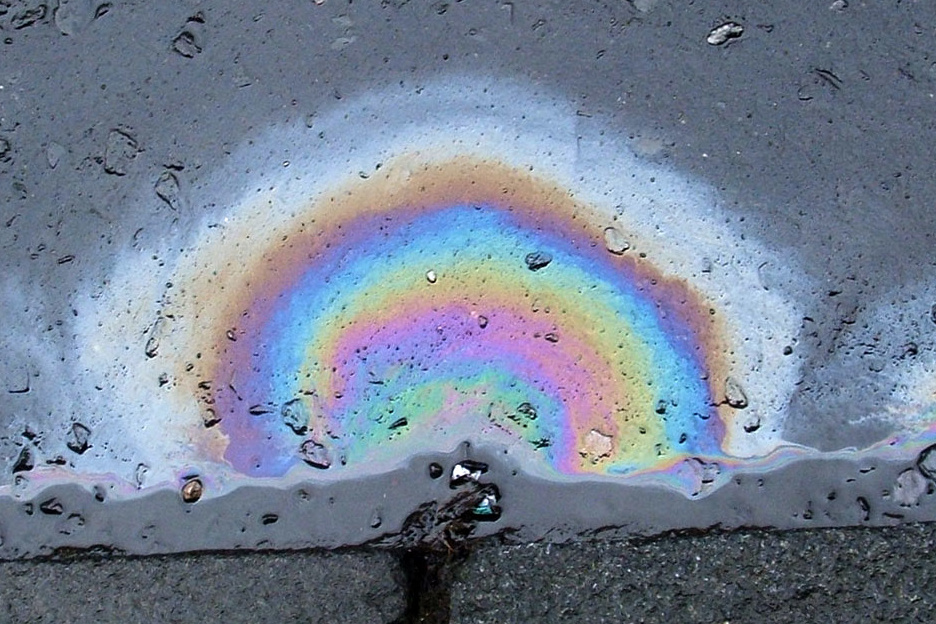
\includegraphics[width=7truecm]{slike/06_photo_oil.jpg}\hfill
\includegraphics[width=7truecm]{slike/06_photo_soap.jpg}\newline

\includegraphics[width=7truecm]{slike/06_photo_zrak.jpg}\hfill
\includegraphics[width=7truecm]{slike/06_photo_us.jpg}
\caption{Interferenca na tanki plasti motornega olja na vodi, 
milnice v zraku, tanke plasti zraka med objektnima stekelcema 
v beli in rdeči svetlobi ter interferenca
na krilih žuželke. Foto listne uši: Miran Pflaum.}
\vglue-8truemm
\label{fig:06_Photos}
\end{figure}

\end{example}

\section{Večkratni odboj na tanki plasti}\index{Interferenca na tanki plasti}\index{Odboj na tanki plasti}
Spoznali smo interferenco na tanki plasti, pri čemer
smo upoštevali le delni valovanji, ki sta se odbili na zgornji in 
spodnji meji tanke plasti. Odboje višjih redov smo zanemarili.

Zdaj se osredotočimo na interferenco velikega števila delnih 
valovanj, ki nastanejo z delitvijo amplitude na tanki plasti dielektrika.
Naj tako kot v prejšnjem razdelku ravno valovanje vpada na tanko plast 
snovi z lomnim količnikom $n_2$, lomni količnik okolice pa naj bo enak $n_1$. 
Ponovno se omejimo na primer TE polariziranega valovanja, pri katerem
je smer jakosti električnega polja pravokotna na vpadno ravnino 
(slika~\ref{fig:06_plastmulti}). Ob vpadu na mejo med snovema se del 
svetlobe odbije, del pa lomi po lomnem zakonu (enačba~\ref{eq:lomnizakon}).
Za razliko od prej bomo zdaj upoštevali vsoto vseh prepuščenih valov, 
ki prehajajo skozi tanko plast, z ustrezno zmanjšano amplitudo.
\begin{figure}[ht]
\centering
\def\svgwidth{70truemm} 
\input{slike/06_plastmulti.pdf_tex}
\caption{Prehod svetlobe skozi tanko plast dielektrika. Delni žarki, ki prehajajo
skozi plast, med seboj interferirajo, zato je intenziteta prepuščene svetlobe odvisna
od debeline plasti $d$, lomnih količnikov plasti $n_2$ in okolice $n_1$ ter vpadnega 
kota $\alpha$. }
\vglue-2truemm
\label{fig:06_plastmulti}
\end{figure}

Zanima nas gostota prepuščenega svetlobnega toka $j$ v odvisnosti od 
lomnih količnikov $n_1$ in $n_2$, vpadnega kota $\alpha$ in debeline plasti $d$ pri dani
vpadni gostoti toka $j_0$. Spomnimo se, da za TE polarizirano valovanje
amplitudno prepustnost zapišemo z enačbo~(\ref{eq:TEr}), amplitudno odbojnost
pa z enačbo~(\ref{eq:TEt}). Ob vstopu v tanko plast tako velja:
\begin{equation}
r_{12} = \frac{n_1\cos \alpha - n_2\cos \beta}{n_1\cos \alpha + n_2\cos \beta}\qquad 
\mathrm{in}\qquad t_{12} = 1+r_{12},
\label{eq:06_35}
\end{equation}
ob izstopu valovanja iz tanke plasti pa:
\begin{equation}
r_{21} = \frac{n_2\cos \beta - n_1\cos \alpha}{n_2\cos \beta + n_1\cos \alpha}\qquad 
\mathrm{in}\qquad t_{21} = 1+r_{21},
\label{eq:06_36}
\end{equation}
pri čemer smo upoštevali, da je izhodni kot enak vpadnemu kotu $\alpha$. 

Posamezne prispevke jakosti 
električnega polja na izhodni strani zapišemo kot:
\begin{align}
E_1 &= E_0\,t_{12}\,t_{21},\\
E_2 &= E_0\,t_{12}\left(r_{21}\,r_{21}\,e^{i\phi}\right)t_{21},\\
E_3 &= E_0\,t_{12}\left(r_{21}\,r_{21}\,e^{i\phi}\right)
\left(\,r_{21}\,r_{21}\,e^{i\phi}\right)t_{21},\\
&...\nonumber\\
E_{N+1} &= E_0t_{12}\,\left(r_{21}\,r_{21}\,e^{i\phi}\right)^Nt_{21}.
\label{eq:06_37}
\end{align}
Upoštevali smo tudi fazni zamik med dvema sosednjima izhodnima valovanjema, do katerega
pride zaradi razlike v prepotovani poti (enačba~\ref{eq:06_34}):
\begin{equation}
\phi = 2k_0 n_2 d \cos \beta.
\label{eq:06_38}
\end{equation}
Celotno prepuščeno polje $E_t$ zapišemo kot vsoto vseh prispevkov (enačba~\ref{eq:06_37}) 
in dobimo:
\begin{align}
E_t &= E_1+E_2+E_3+... \nonumber \\
&= E_0\, t_{12}\,t_{21}\,\left(1 + r_{21}^2 e^{i\phi} + r_{21}^4 e^{2i\phi} 
+ r_{21}^6 e^{3i\phi} + ... \right)\!\!.
\label{eq:06_39}
\end{align}
Geometrijsko vrsto v oklepaju seštejemo in za jakost prepuščenega polja dobimo:
\begin{equation}
E_t = E_0 t= E_0 t_{12}t_{21}\frac{1}{1-r_{21}^2e^{i\phi}},
\label{eq:06_40}
\end{equation}
pri čemer smo vpeljali $t$ kot amplitudno prepustnost plasti. Ker sta lomni\index{Amplitudna prepustnost!{tanke plasti}}
količnik snovi in smer širjenja svetlobe na izhodni strani enaka kot na vpadni, je 
prepustnost $T$, ki označuje razmerje med gostoto prepuščenega in vpadnega svetlobnega\index{Prepustnost!{tanke plasti}}
toka, kar enaka $|t|^2$:
\begin{equation}
T = \frac{j}{j_0} = |t|^2= \frac{t_{12}^2t_{21}^2}{\left(1-r_{21}^2e^{i\phi}\right)
\left(1-r_{21}^2e^{-i\phi}\right)}.
\label{eq:06_41}
\end{equation}
Upoštevali smo, da je tanka plast dielektrična in so zato vrednosti amplitudnih 
prepustnosti in odbojnosti realne. Zapišemo še odbojnost $R = r_{21}^2$ in upoštevamo\index{Odbojnost!{tanke plasti}}
zveze med amplitudnimi prepustnostmi in odbojnostmi:
$t_{21} = 1+r_{21}$ in $t_{12} = 1+r_{12} = 1-r_{21}$. Dobimo:
\begin{equation}
T = \frac{\left(1-R\right)^2}{1 + R^2 - 2R\cos \phi}.
\label{eq:06_42}
\end{equation}
Imenovalec preoblikujemo, tako da upoštevamo zvezo $\cos(2x) = 1-2\sin^2x$:
\begin{equation}
1 + R^2 - 2R\cos \phi = 1+R^2 - 2R(1-2\sin^2(\phi/2)) = (1-R)^2 + 4R \sin^2(\phi/2).
\label{eq:06_43}
\end{equation}
Preoblikovan izraz vstavimo v enačbo~(\ref{eq:06_42}), jo delimo s števcem in 
dobimo končen izraz za prepustnost tanke plasti:
\boxeq{eq:FP}{
T = \frac{1}{1 + \frac{4R}{\left(1-R\right)^2} \sin^2(\phi/2)}.
}
Spomnimo, da je $R = r_{21}^2$ podan z enačbo~(\ref{eq:06_36}), $\phi$ pa z 
enačbo~(\ref{eq:06_38}). 

Izračunano odvisnost $T(\phi)$ imenujemo tudi Airyjeva\index{Airyjeva funkcija}
funkcija.\footnote{Ločiti je treba Airyjevo funkcijo za prepustnost 
na tanki plasti (enačba~\ref{eq:FP}) od Airyjeve funkcije v matematiki in tudi 
od Airyjevega diska, ki smo ga vpeljali pri uklonu na okrogli odprtini 
(enačba~\ref{eq:uklonAiry}). Gre za povsem drugačne funkcijske odvisnosti.}
Airyjeva funkcija, ki se v odvisnosti od parametra $\phi$ periodično spreminja
med 0 in 1, zavzame največje vrednosti, kadar je izpolnjen pogoj $\phi = 2 \pi N$, 
pri čemer je $N$ celo število. Zapisani pogoj je ekvivalenten zahtevi, da je  
fazna razlika med dvema prepuščenima delnima valovanjema enaka večkratniku 
števila $2\pi$ in zato prepuščeni delni valovanji med seboj konstruktivno 
interferirata. Takrat je vsa vpadna svetloba prepuščena ($T=1$) in 
odbojnost tanke plasti za dano valovno dolžino je enaka nič. Tanka plast torej 
deluje kot frekvenčni filter, saj pri dani debelini dobro prepušča le valovanja
s točno določenimi valovnimi dolžinami, ostala valovanja pa se od tanke plasti 
odbijejo.

Vpeljimo še en parameter, to je koeficient finese:\index{Koeficient finese}
\begin{equation}
F = \frac{4R}{(1-R)^2}.
\label{eq:06_44d}
\end{equation}
Vrednost koeficienta finese določa kontrast prepustnosti svetlobe skozi tanko
plast (slika~\ref{fig:06_FP1}). Odvisen je zgolj od odbojnosti na meji
med tanko plastjo in okolico $R$, ta pa od lomnih količnikov plasti in okolice
ter vpadnega kota na mejno ploskev. Že pri razmeroma majhni odbojnosti na mejni
ploskvi (npr. $R=0,3$) so vrhovi največje prepustnosti jasno vidni, pri večji 
odbojnosti (npr. $R=0,9$) pa postanejo vrhovi izredno ozki.
\begin{figure}[ht]
\centering
\def\svgwidth{110truemm} 
\input{slike/06_FP1.pdf_tex}
\caption{Odvisnost prepustnosti tanke plasti od parametra faznega zamika $\phi$
za različne vrednosti koeficienta finese $F$: modra $R = 0,3$ in $F=2,45$; 
zelena $R=0,5$ in $F=8$ ter rdeča $R=0,9$ in $F=3600$.}
\label{fig:06_FP1}
\end{figure}

\section{Fabry-Perotov interferometer}\index{Fabry-Perotov interferometer}\index{Interferometer!{Fabry-Perotov}}
Naprava, ki temelji na selektivni prepustnosti tanke plasti dielektrika, je 
Fabry-Perotov interferometer. Imenuje se po francoskih fizikih Charlesu Fabryju (1867--1945)\index{Fabry, Charles}
in Alfredu Perotu (1863--1925), ki sta napravo razvila leta 1899. Fabry-Perotov interferometer\index{Perot, Alfred}
je navadno sestavljen iz dveh premičnih delno prepustnih ravnih zrcal, med katerima
je zelo tanka reža. S spreminjanjem razmika med zrcaloma (in s tem debeline vmesne tanke
plasti zraka) izbiramo valovno dolžino
valovanja, ki ga interferometer popolnoma prepušča. Uporabljamo ga predvsem
za spektralno analizo oziroma spektroskopijo, na primer v astronomiji. 

Podobna naprava je Fabry-Perotov\index{Fabry-Perotov etalon}
etalon. Ta je navadno sestavljen iz ploščice dielektrika, katere debeline ne 
moremo spreminjati. Stranicam dielektrika lahko z dodatnim nanosom povečamo
odbojnost. Fabry-Perotovi etaloni so uporabni med drugim v optičnih 
telekomunikacijah in za spektralno filtracijo svetlobe pri izdelavi laserjev.

V prejšnjem razdelku smo izpeljali prepustnost valovanja skozi plast
dielektrika (enačba~\ref{eq:FP}), pri čemer smo intenziteto odbitega
oziroma prepuščenega valovanja na mejnih ploskvah izračunali z uporabo
Fresnelovih enačb. Povsem enak rezultat dobimo, če namesto ploščice 
dielektrika obravnavamo prepustnost skozi tanko plast zraka, omejeno
z dvema delno prepustnima ravnima zrcaloma. V tem primeru sta
vpadni kot $\alpha$ in lomni kot $\beta$  približno enaka, $n_2 \approx 1$,
odbojnost $R$ pa je enaka odbojnosti delno prepustnih zrcal. Privzamemo 
še, da svetloba na interferometer vpada pravokotno, in izraz za prepustnost
prepišemo v:
\begin{equation}
T(\omega) = \frac{1}{1 + \frac{4R}{\left(1-R\right)^2} \sin^2(\omega d n_2/c_0)}.
\label{eq:06_44}
\end{equation}

Pomemben parameter pri Fabry-Perotovem interferometru je tako imenovano prosto\index{Prosto spektralno območje}
spektralno območje ($FSR$ -- {\it Free Spectral Range}). 
Gre za območje spektra med dvema zaporednima vrhoma (slika~\ref{fig:06_FP2})
in določa širino spektra, ki jo lahko s tako napravo analiziramo. 
Prosto spektralno območje izračunamo iz pogoja, da se fazna razlika $\phi$ spremeni
za $2\pi$:
\begin{equation}
\Delta \phi = 2 \pi = \Delta \left(2 \omega_\mathrm{FSR} d n_2/c_0\right)= 
2 \Delta \omega_\mathrm{FSR} dn_2/c_0
\label{eq:06_45}
\end{equation}
in dobimo:
\boxeq{eq:FSR}{
\Delta \nu_\textrm{FSR}=\frac{c_0}{2dn_2}.
}
\begin{example}{\bf Prosto spektralno območje.}
Obravnavajmo Fabry-Perotov interferometer, ki je sestavljen iz dveh ravnih zrcal, med 
katerima je tanka plast zraka. Položaj zrcal zelo natančno nastavljamo s piezoelektričnim 
mehanizmom in nastavimo debelino reže na $d=0,1~\si{mm}$. Izračunajmo
prosto spektralno območje za tak interferometer (enačba~\ref{eq:FSR}):
\begin{equation}
\Delta \nu_\textrm{FSR} = \frac{3 \cdot 10^8~\si{m/s}}{2 \cdot 10^{-4}~\si{m}} \sim 10^{12}~\si{Hz}.
\label{eq:06_51d}
\end{equation}
S takim interferometrom lahko analiziramo spektralne podrobnosti 
v intervalu širine $1~\si{THz}$, kar  v območju vidne svetlobe
ustreza $\Delta \lambda_\textrm{FSR} \sim 1~\si{nm}$. Navadno zato uporabimo dodatne filtre, 
s katerimi iz celotnega spektra najprej osamimo le svetlobo v bližini opazovanega dela in šele nato
natančno analiziramo s Fabry-Perotovim interferometrom. 
\end{example}
\vglue-5truemm
\begin{remark}
Primer uporabe Fabry-Perotovega interferometra 
je opazovanje spektra svetlobe, ki jo izseva vodikov atom. Najsvetlejša
spektralna črta H$_\alpha$ ustreza prehodu elektronov iz stanja 
$n=3$ v stanje $n=2$ (Balmerjeva serija) z valovno dolžino $656,28~\si{nm}$.
Podrobnejša analiza pokaže, da je črta sestavljena iz dveh ločenih črt, ki nastaneta
kot posledica sklopitve spin-tir. Razlika med njima je le $0,016~\si{nm}$, vendar jo
z interferometrom lahko izmerimo. Opazovanje vodikovega  H$_\alpha$ dubleta 
je bilo en prvih eksperimentalnih dokazov za obstoj elektronskega spina.
\end{remark}

Drugi pomemben parameter pri tovrstni spektroskopiji je širina transmisijskih
vrhov (slika~\ref{fig:06_FP2}).
Ta namreč določa, kako natančno lahko analiziramo signal znotraj prostega 
spektralnega območja, in torej določa ločljivost Fabry-Perotovega interferometra. 
Širino posameznega vrha $\delta \nu_{1/2}$ izračunamo iz vrednosti frekvence, pri kateri pade 
prepustnost interferometra na $T=0,5$. Celotno širino pri polovični
višini pogosto označimo tudi z angleško kratico $FWHM$ ({\it Full Width at Half
Maximum}).\index{FWHM}
\begin{figure}[ht]
\centering
\def\svgwidth{100truemm} 
\input{slike/06_FP2.pdf_tex}
\caption{Prosto spektralno območje $\Delta \nu_{\rm FSR}$
je interval med dvema zaporednima vrhoma prepustnosti.
Širino vrha $\delta \nu_{1/2}$ po dogovoru določimo na polovični prepustnosti. 
Primer je narisan za $R=0,5$.}
\label{fig:06_FP2}
\vglue-4truemm
\end{figure}

Širino vrha izračunamo iz pogoja $T=0,5$ (enačba~\ref{eq:FP}):
\begin{equation}
T = \frac{1}{1 + \frac{4R}{\left(1-R\right)^2} \sin^2(\phi/2)} = \frac{1}{2} \qquad
\Longrightarrow \qquad \frac{4R}{\left(1-R\right)^2} \sin^2(\phi/2) = 1.
\label{eq:06_46}
\end{equation}
Privzamemo, da so vrhovi ozki in sinus razvijemo za majhne vrednosti:
\begin{equation}
\phi/2 = \sqrt{\frac{\left(1-R\right)^2}{4R}}.
\label{eq:06_47}
\end{equation}
Fazni zamik na polovični vrednosti vrha je potem:
\begin{equation}
\phi_{1/2} = \frac{1-R}{\sqrt{R}}.
\label{eq:06_48}
\end{equation}
Vstavimo izraz za fazno razliko $\phi$ (enačba~\ref{eq:06_34}) in 
za celotno širino vrha na polovični višini dobimo zvezo:
\begin{equation}
2k_0 n_2 d = \frac{4\pi \nu n_2 d}{c_0} = 2\frac{1-R}{\sqrt{R}},
\label{eq:06_49}
\end{equation}
od koder sledi:
\begin{equation}
\delta \nu_{1/2} = \frac{1-R}{2\sqrt{R}} \frac{c_0}{\pi n_2 d}.
\label{eq:06_50}
\end{equation}
\vglue-8truemm
\begin{remark}
Pogosto govorimo o finesi interferometra, ki jo vpeljemo kot\index{Finesa}
kvocient med prostim spektralnim območjem in širino vrha. Izračunamo jo 
z upoštevanjem enačb~(\ref{eq:FSR} in \ref{eq:06_50}):
\begin{equation}
\mathcal{F} = \frac{\Delta \nu_\textrm{FSR}}{\delta \nu_{1/2}}  = \frac{\pi}{2}\sqrt{F}.
\label{eq:06_51}
\end{equation}
\end{remark}

\section{Večplastni nanosi}\index{Interferenca!{večplastni nanos}}
Prepustnost tanke plasti je razmeroma preprosto izračunati. Vendar se račun hitro
zaplete, kadar je tankih plasti več. Namesto seštevanja prispevkov 
posameznih odbojev valovanja na mejah med plastmi zato raje zapišemo celotno polje 
v neki plasti, prehod iz ene plasti v drugo pa opišemo s prehodno matriko.
Zaradi enostavnosti se omejimo zgolj na pravokotni 
vpad svetlobe na večplastno strukturo, polarizacija pa ni pomembna, saj 
je v tem primeru obravnava TE in TM polariziranega valovanja enaka.

Naj bodo polja na levih 
robovih plasti označena z $E_N$, na desnih robovih plasti pa z $\tilde{E}_N$. 
V vseh plasteh, razen na izhodni plasti, sta prisotni dve valovanji: prvo se širi
v desno in drugo v levo. Jakosti električnega polja, ki pripadajo slednjemu
valovanju, označimo s črtico (slika~\ref{fig:06_prehodneM}).
\begin{figure}[ht]
\centering
\def\svgwidth{100truemm} 
\input{slike/06_prehodneM.pdf_tex}
\caption{K izračunu prehoda skozi večplastni nanos}
\label{fig:06_prehodneM}
\end{figure}

Poglejmo najprej, kako z matričnim pristopom opišemo povezavo med poljema na 
meji $1\rightarrow 2$. Robni pogoji (enačba~\ref{eq:RPE}) zahtevajo, 
da se na meji ohranja tangentna komponenta jakosti električnega polja. Ker je
vpad pravokoten, se ohranja celotna jakost električnega polja. Izrazimo 
prepuščeno polje $E_2$ s poljema $\tilde{E}_1$ in $E_2'$, tako da upoštevamo
amplitudno prepustnost in odbojnost na meji (enačbe~\ref{eq:06_35} in \ref{eq:06_36}):
\begin{equation}
E_2 = t_{12}\tilde{E}_1 + r_{21}E_2'.
\label{eq:06_53}
\end{equation}
Podobno zapišemo tudi odbito polje $\tilde{E}_1'$ kot:
\begin{equation}
\tilde{E}_1' = t_{21}E_2' + r_{12}\tilde{E}_1.
\label{eq:06_54}
\end{equation}
Iz enačbe~(\ref{eq:06_54}) izrazimo $E_2'$:
\begin{equation}
E_2' = \frac{1}{t_{21}}\left(\tilde{E}_1' - r_{12}\tilde{E}_1\right) = 
\frac{1}{t_{21}}\left(\tilde{E}_1' + r_{21}\tilde{E}_1\right),
\label{eq:06_54a}
\end{equation}
pri čemer smo upoštevali, da velja $r_{12} = - r_{21}$. Izračunano polje vstavimo v 
enačbo~(\ref{eq:06_53}) in dobimo:
\begin{equation}
E_2 = t_{12}\tilde{E}_1 -\frac{r_{12}r_{21}}{t_{21}}\tilde{E}_1 + 
\frac{r_{21}}{t_{21}}\tilde{E}_1'.
\label{eq:06_55}
\end{equation}
Izraz preoblikujemo:
\begin{equation}
E_2 = \frac{1}{t_{21}} \left(t_{12}t_{21}\tilde{E}_1 -r_{12}r_{21}\tilde{E}_1 + 
r_{21}\tilde{E}_1'\right)\!\!.
\label{eq:06_55a}
\end{equation}
Izračunajmo zvezo med koeficienti prepustnosti in odbojnosti:
\begin{equation}
t_{12}t_{21} - r_{12}r_{21} = (1+r_{12})(1+r_{21}) - r_{12}r_{21} = 
(1+r_{12})(1-r_{12}) + r_{12}^2 = 1,
\label{eq:06_56}
\end{equation}
s čimer enačbo~(\ref{eq:06_55a}) poenostavimo v:
\begin{equation}
E_2 = \frac{1}{t_{21}}\left(\tilde{E}_1 + r_{21}\tilde{E}_1'\right).
\label{eq:06_57}
\end{equation}
Tako smo z enačbami povezali oba prispevka k polju na desni strani meje s poljem
levo od meje.  

Sestavimo zdaj 2D vektorja iz valovanj, ki se širita v desno in v levo, in zvezi
med njimi (enačbi~\ref{eq:06_54a} in \ref{eq:06_57}) strnjeno zapišemo kot:
\begin{equation}
\left[\begin{array}{c}
E_{2}\\
E_{2}'\\
\end{array}\right] =
\frac{1}{t_{21}}
\left[\begin{array}{cc}
1& r_{21}\\
r_{21}& 1\\
\end{array}\right]\cdot
\left[\begin{array}{c}
\tilde{E}_1\\
\tilde{E}_1'\\
\end{array}\right]\!\!.
\label{eq:06_58}
\end{equation}
Kot bomo videli pozneje, je priročno obrniti smer gledanja, tako da polje na 
levi izrazimo s poljem na desni strani meje. Obrnjene enačbe strnjeno zapišemo z matriko:
\begin{equation}
\left[\begin{array}{c}
\tilde{E}_{1}\\
\tilde{E}_{1}'\\
\end{array}\right] =
\frac{1}{t_{12}}
\left[\begin{array}{cc}
1& r_{12}\\
r_{12}& 1\\
\end{array}\right]\cdot
\left[\begin{array}{c}
E_2\\
E_2'\\
\end{array}\right]\!\!.
\label{eq:06_59}
\end{equation}
Zapisani izraz posplošimo in zapišemo povezavo na meji med plastjo 
$N-1$ in plastjo $N$:
\boxeq{eq:prehodnaM}{
\left[\begin{array}{c}
\tilde{E}_{N-1}\\
\tilde{E}_{N-1}'\\
\end{array}\right] =
\frac{1}{t_{N-1,N}}
\left[\begin{array}{cc}
1& r_{N-1,N}\\
r_{N-1,N}& 1\\
\end{array}\right]\cdot
\left[\begin{array}{c}
E_N\\
E_N'\\
\end{array}\right] = 
M_{N-1,N}\left[\begin{array}{c}
E_N\\
E_N'\\
\end{array}\right]\!\!.
}

Na podoben način lahko s prehodno matriko povežemo tudi polja na 
levi in desni strani znotraj posamezne plasti. Razlika
je le v fazi, ki jo valovanje pridobi med premikom po plasti. 
Če je debelina $N$-te plasti $d_N$ in njen
lomni količnik $n_N$, zapišemo zvezi:
\begin{equation}
\tilde{E}_N = E_N e^{i k_0 n_N d_N}
\label{eq:06_60}
\end{equation}
in 
\begin{equation}
E_N' = \tilde{E}_N' e^{i k_0 n_N d_N}.
\label{eq:06_61}
\end{equation}
V matričnem zapisu je premik po posamezni plasti enak:
\begin{equation}
\left[\begin{array}{c}
E_{N}\\
E_{N}'\\
\end{array}\right] =
\left[\begin{array}{cc}
e^{-i\delta}& 0\\
0& e^{i\delta}\\
\end{array}\right]\cdot
\left[\begin{array}{c}
\tilde{E}_N\\
\tilde{E}_N'\\
\end{array}\right] = 
P_{N}\left[\begin{array}{c}
\tilde{E}_N\\
\tilde{E}_N'\\
\end{array}\right]\!\!,
\label{eq:06_62}
\end{equation}
pri čemer smo vpeljali fazni zamik $\delta = k_0 n_N d_N$.

Zapis z matrikami je priročen predvsem v primerih, ko imamo sistem več tankih plasti
z različnimi debelinami in lomnimi količniki. Za vsako mejno plast zapišemo
ustrezno prehodno matriko, prav tako za vsak premik znotraj posamezne plasti. 
Povezavo med vhodnim poljem ($E_0$) in izhodnim poljem ($E_i$) 
izračunamo tako, da vse zapisane matrike 
zmnožimo v pravilnem vrstnem redu. Pri tem 
prehod obravnavamo od izhodne (desne) strani proti vpadni (levi) strani, saj vemo, da na
izstopni strani svetlobe, ki bi se širila proti levi, ni. 
Na splošno je zapis oblike:
\begin{equation}
\left[\begin{array}{c}
E_{0}\\
E_{0}'\\
\end{array}\right] = 
M_{01}
P_1
M_{12}
P_2
M_{23}
P_3 ... M_{N,i}
\left[\begin{array}{c}
E_i\\
0\\
\end{array}\right] =
A
\left[\begin{array}{c}
E_i\\
0\\
\end{array}\right]\!\!,
\label{eq:06_63}
\end{equation}
pri čemer $A$ označuje prehodno matriko celotnega sistema. Ko enkrat 
poznamo matriko $A$, lahko hitro izračunamo amplitudno 
prepustnost in odbojnost večplastnega sistema. Matriko zapišemo
po komponentah:
\begin{equation}
\left[\begin{array}{c}
E_{0}\\
E_{0}'\\
\end{array}\right] =
\left[\begin{array}{cc}
A_{11}& A_{12}\\
A_{21}& A_{22}\\
\end{array}\right]\cdot
\left[\begin{array}{c}
E_i\\
0\\
\end{array}\right]\!\!,
\label{eq:06_64}
\end{equation}
od koder razberemo amplitudno prepustnost $t$ in amplitudno odbojnost
$r$:\index{Amplitudna prepustnost!{večplastnega nanosa}}\index{Amplitudna odbojnost!{večplastnega nanosa}}
\boxeq{eq:plasti}{
t = \frac{E_i}{E_0} = \frac{1}{A_{11}} \qquad \mathrm{in} \qquad 
r = \frac{E_0'}{E_0} = \frac{A_{21}}{A_{11}}.
}
Tako na preprost način izračunamo prepustnost in odbojnost
večplastnih nanosov, vendar ne smemo pozabiti, 
da je celoten račun narejen ob predpostavki pravokotnega vpada.

\begin{example}{\bf Matrična obravnava Fabry-Perotovega etalona.}\index{Fabry-Perotov etalon}
Uporabimo matrični pristop za izračun prehoda svetlobe skozi tanko plast dielektrika
(Fabry-Perotov etalon). Naj bodo debelina plasti $d$, njen lomni količnik $n_1$, 
lomni količnik okolice pa $n_0$. V tem primeru moramo zapisati tri matrike:
eno za prehod v plast $M_{01}$, drugo za prehod znotraj plasti $P_1$ in 
tretjo za prehod iz plasti $M_{10}$:
\begin{equation}
\left[\begin{array}{c}
E_{0}\\
E_{0}'\\
\end{array}\right] = 
A
\left[\begin{array}{c}
E_i\\
0\\
\end{array}\right] = 
M_{01}P_1M_{10}
\left[\begin{array}{c}
E_i\\
0\\
\end{array}\right]\!\!.
\label{eq:06_65}
\end{equation}
Uporabimo matriki za prehod skozi mejo (enačba~\ref{eq:06_59}) 
in za premik po snovi (enačba~\ref{eq:06_62}). Zapišemo:
\begin{equation}
A =
\frac{1}{t_{01}}
\left[\begin{array}{cc}
1& r_{01}\\
r_{01}& 1\\
\end{array}\right]\cdot
\left[\begin{array}{cc}
e^{-i\delta}& 0\\
0& e^{i\delta}\\
\end{array}\right]\cdot
\frac{1}{t_{10}}
\left[\begin{array}{cc}
1& r_{10}\\
r_{10}& 1\\
\end{array}\right]\!\!,
\label{eq:06_66}
\end{equation}
pri čemer je fazni zamik $\delta = k_0 n_1 d$. Matrike zmnožimo in dobimo:
\begin{equation}
A =
\frac{1}{t_{01}t_{10}}
\left[\begin{array}{cc}
e^{-i\delta}+r_{01}r_{10}e^{i\delta}& r_{10}e^{-i\delta}+r_{01}e^{i\delta} \\
r_{01}e^{-i\delta}+r_{10}e^{i\delta} & r_{01}r_{10}e^{-i\delta}+ e^{i\delta}\\
\end{array}\right]\!\!.
\label{eq:06_67}
\end{equation}
Ko poznamo celotno matriko $A$, lahko iz nje razberemo koeficient prepustnosti 
(enačba~\ref{eq:plasti}):
\begin{equation}
t = \frac{1}{A_{11}} = \frac{t_{01}t_{10}}{e^{-i\delta}+r_{01}r_{10}e^{i\delta}} = 
\frac{1-r_{01}^2}{e^{-i\delta}\left(1-r_{01}^2e^{2i\delta}\right)},
\label{eq:06_68}
\end{equation}
pri čemer smo upoštevali enačbe~(\ref{eq:06_35} in \ref{eq:06_36}) in zvezo
$r_{01} = r_{10}$. 

Vpeljemo še odbojnost na meji $R = r_{01}^2$ in fazni zamik 
$\phi = 2 \delta = 2 k_0 n_2 d$. Izračunamo prepustnost, pri čemer upoštevamo 
enačbo~(\ref{eq:06_44}):
\begin{equation}
T = |t|^2 = \frac{\left(1-R\right)^2}{\left(1 - Re^{2i\delta}\right)\left(1 -
Re^{-2i\delta}\right)} = \frac{\left(1-R\right)^2}{1 + R^2 - 2R\cos \phi}=
\frac{1}{1 + \frac{4R}{\left(1-R\right)^2} \sin^2(\phi/2)}.
\label{eq:06_69}
\end{equation}
Izpeljali smo prepustnost 
tanke plasti dielektrika, ki je po pričakovanju povsem enaka prepustnosti 
Fabry-Perotovega interferometra, izračunani s seštevanjem delnih valovanj (enačba~\ref{eq:FP}).

\end{example}

\begin{example}{\bf Antirefleksni nanos.}\index{Antirefleksni nanos}
Kadar želimo zmanjšati odboj svetlobe pri vpadu na mejo dveh snovi, uporabimo
antirefleksne nanose. To so praviloma zelo tanke plasti iz neke tretje snovi, 
s katerimi dosežemo zmanjšanje odbojnosti in tako povečanje prepustnosti. Poglejmo, 
kako lahko dosežemo, da se nič vpadne svetlobe ne odbije in je $R=0$. 

V tem primeru naj svetloba iz snovi z lomnim količnikom $n_1$ vpada na tanek antirefleksni
nanos debeline $d$ z lomnim količnikom $n_2$ in potem prehaja v snov z lomnim količnikom 
$n_3$. Matrika, ki opisuje prehod skozi opisani sistem, je produkt dveh prehodov skozi
mejo in enega premika po snovi:
\begin{equation}
A = 
\frac{1}{t_{12}}
\left[\begin{array}{cc}
1& r_{12}\\
r_{12}& 1\\
\end{array}\right]\cdot
\left[\begin{array}{cc}
e^{-i\delta}& 0\\
0& e^{i\delta}\\
\end{array}\right]\cdot
\frac{1}{t_{23}}
\left[\begin{array}{cc}
1& r_{23}\\
r_{23}& 1\\
\end{array}\right]\!\!.
\label{eq:06_70}
\end{equation}
Matrike zmnožimo in dobimo:
\begin{equation}
A =
\frac{1}{t_{12}t_{23}}
\left[\begin{array}{cc}
e^{-i\delta}+r_{12}r_{23}e^{i\delta}& r_{23}e^{-i\delta}+r_{12}e^{i\delta} \\
r_{12}e^{-i\delta}+r_{23}e^{i\delta} & r_{12}r_{23}e^{-i\delta}+ e^{i\delta}\\
\end{array}\right]\!\!.
\label{eq:06_71}
\end{equation}
Prepustnost sistema izračunamo iz enačbe~(\ref{eq:plasti}), pri čemer s faktorjem $n_3/n_1$ 
upoštevamo, da se po prehodu valovanje širi po drugačni snovi:
\begin{equation}
T =\frac{n_3}{n_1} |t|^2 = \frac{n_3}{n_1} \left\rvert \frac{1}{A_{11}}\right\rvert^2 = 
\frac{n_3}{n_1} \cdot  \frac{t_{12}^2t_{23}^2}{1+ r_{12}^2r_{23}^2+2r_{12}r_{23}\cos\phi},
\label{eq:06_72}
\end{equation}
pri čemer je $\phi = 2k_0n_2d$. Prepustnost $T$ je največja, kadar je imenovalec najmanjši in 
$\cos \phi = -1$. Iz tega pogoja izračunamo debelino  nanosa:
\begin{equation}
\phi = 2 \frac{2\pi}{\lambda} n_2 d = \pi \qquad \Longrightarrow \qquad d = \frac{\lambda}{4n_2}.
\label{eq:06_73}
\end{equation}
Najmanjša potrebna debelina antirefleksnega nanosa je torej četrtina valovne dolžine valovanja v nanosu.
Druge rešitve (večje debeline) dobimo z upoštevanjem periodičnosti sinusne funkcije. Rezultat je pričakovan,
saj se pri izračunani debelini valovanje, ki je odbito od prve meje med plastmi, destruktivno sešteje z 
valovanjem, odbitim na drugi meji. Celotno odbito valovanje je enako nič in vsa svetloba je prepuščena. 

Izračunajmo še odbojnost z upoštevanjem enačbe~(\ref{eq:plasti}):
\begin{equation}
R = |r|^2 = \left\rvert \frac{A_{21}}{A_{11}}\right\rvert^2 = 
\left\rvert\frac{r_{12}e^{-i\delta}+r_{23}e^{i\delta}}{e^{-i\delta}+r_{12}r_{23}e^{i\delta}}\right\rvert^2\!\!.
\label{eq:06_74}
\end{equation}
Vstavimo izračunano debelino nanosa (enačba~\ref{eq:06_73}) in odbojnost poenostavimo v:
\begin{equation}
R = \frac{r_{12}^2+r_{23}^2-2r_{12}r_{23}}{1-r_{12}^2r_{23}^2} = \frac{(r_{12}-r_{23})^2}{(1-r_{12}r_{23})^2}.
\label{eq:06_75}
\end{equation}
Da dosežemo popolno prepustnost svetlobe in nič odboja, mora biti $R=0$. To velja, kadar je $r_{12} = r_{23}$
oziroma izraženo z lomnimi količniki snovi (enačba~\ref{eq:06_35}):
\begin{equation}
\frac{n_1-n_2}{n_1+n_2} = \frac{n_2-n_3}{n_2+n_3}.
\label{eq:06_76}
\end{equation}
Pri danih lomnih količnikih $n_1$ in $n_3$ izračunamo lomni količnik antirefleksnega nanosa in pogoja, 
da se na plasti svetloba ne odbija, strnjeno zapišemo kot:
\boxeq{eq:antirefleks}{
n_2 = \sqrt{n_1n_3} \qquad \mathrm{in} \qquad d = \frac{\lambda}{4n_2}.
}
Kadar je debelina nanosa enaka četrtini valovne dolžine v nanosu, njen lomni količnik pa je 
geometrijska sredina lomnih količnikov snovi na obeh straneh nanosa, se svetloba ne odbija. 

Antirefleksni nanosi so zelo praktično uporabni, saj zmanjšajo odbojnost in povečajo intenziteto prepuščenega signala. 
Uporabljamo jih med drugim na korekcijskih očalih vida, na lečah, v mikroskopih ali teleskopih in 
na sončnih celicah. Ker je razmeroma težko najti snov, ki bi imela lomni količnik enak geometrijski sredini
med lomnim količnikom zraka ($n_1=1$) in stekla ($n_3=1,52$), se za antirefleksne snovi najpogosteje uporablja magnezijev 
fluorid MgF$_2$ z lomnim količnikom $n_2=1,38$. 
\end{example}

\begin{remark}
Odbojnost antirefleksnega nanosa je lahko enaka nič le pri eni valovni dolžini, valovanje z drugačnimi valovnimi 
dolžinami se pa še vedno delno odbije. Prav tako smo pri računu privzeli, da je vpad na mejo med snovmi 
pravokoten. V praksi se zato pogosto uporabljajo bolj zapleteni antirefleksni nanosi, sestavljeni iz več
plasti različnih debelin in z različnimi lomnimi količniki. Tako dosežemo odbojnost, manjšo od $0,5~\%$
na skoraj celotnem vidnem območju.
\end{remark}

\begin{example}{\bf Strukturne barve.}\index{Strukturna barva}
Posebej zanimiv primer večplastnih dielektrikov so periodične strukture. Enodimenzionalne 
nastanejo z izmeničnim nanosom na primer dveh plasti z lomnima količnikoma $n_1$ in $n_2$, 
lahko pa so tudi dvo- ali tridimenzionalne periodične strukture. Za opis širjenja svetlobe v
 takih periodičnih dielektričnih strukturah lahko uporabimo Blochov formalizem za opis elektronskih 
 stanj v periodični 
kristalni mreži. Podobno kot se v kristalih pojavijo dovoljeni energijski pasovi za elektrone 
in med njimi prepovedani pasovi oziroma energijske reže, se v periodičnih strukturah dielektrikov
pojavijo stanja, ki se po snovi širijo, in stanja, ki se ne. Zaradi podobnosti s kristali
govorimo o fotonskih kristalih, za njih pa je značilna velika odbojnost za valovanja s točno
določenimi frekvencami znotraj prepovedanega pasu.\index{Fotonski kristal}

Kadar telo dobi barvo zaradi strukture in ne zaradi barvila, govorimo o strukturni barvi. 
Znani primeri strukturnih barv (fotonskih kristalov) v naravi so krila nekaterih metuljev, 
nekatera peresa ptic (race, pava, vodomca, kolibrija), telesa nekaterih kačjih pastirjev ali hroščkov. 
\begin{figure}[!ht]
\centering
\includegraphics[width=7truecm]{slike/06_metulj.jpg}\hfill
\includegraphics[width=7truecm]{slike/06_vodomec.jpg}\newline

\includegraphics[width=7truecm]{slike/06_pav1.jpg}\hfill
\includegraphics[width=7truecm]{slike/06_pastir.jpg}
\caption{Nekaj primerov strukturne barve v naravi: metuljeva krila (Foto: Garoch, Pixabay), peresa vodomca (Foto:
Timo Schl\"uter, Pixabay), pavje pero in kačji pastir (Foto: Miran Pflaum).}
\label{fig:06_FK}
\end{figure}
 
\end{example}








%\chapterimage{Geometrijska.jpg} % Chapter heading image

\chapter{Koherenca}
\label{chap:Koherenca}
Spoznali bomo koherenco, to je lastnost svetlobe, ki je tesno povezana
s pojavom interference. Obravnavali bomo časovno koherenco in zapisali 
Wiener-Hinčinov izrek ter prostorsko koherenco in z njo povezan 
Van Cittert-Zernikov izrek. Poglavje bomo zaključili z opisom holografije.

Koherenca oziroma koherentne lastnosti svetlobe se nanašajo na obstoj povezave
med fazo elektromagnetnega valovanja na nekem kraju ob nekem času ter njegovo 
fazo na nekem drugem kraju ob nekem drugem času. V poglavjih o 
uklonu (poglavje~\ref{chap:Uklon}) in interferenci (poglavje~\ref{chap:Interferenca})
smo pri zapisu elektromagnetnega valovanja privzeli, da poznamo njegovo fazo 
na vsakem kraju in ob vsakem času, s čimer smo predpostavili, 
da je elektromagnetno valovanje popolnoma koherentno. Jakost
električnega polja v tem primeru zapišemo kot funkcijo $\mathbf{r}$ in $t$ 
v obliki (enačba~\ref{eq:ravnival}):
\beq
\mathbf{E} (\mathbf{r}, t) = \mathbf{E}_0(\mathbf{r}, t) 
e^{i\phi(\mathbf{r}, t)}.
\eeq
V realnih sistemih valovanje
ni nikoli povsem koherentno in prej ali slej se povezava med njegovo 
fazo izgubi. Koherentno valovanje ob interferenci da značilen interferenčni 
vzorec, ki se s časom ne spreminja, nekoherentno valovanje pa ne. Pri  
delno koherentnih valovanjih interferenčne vzorce sicer opazimo, vendar z zmanjšanim
kontrastom. 

\section{Časovna koherenca}
Najprej bomo opisali časovno koherenco, ki jo imenujemo tudi longitudinalna 
oziroma vzdolžna koherenca. Časovna koherenca povezuje valovanje ob dveh različnih 
časih. Za opis se omejimo na monokromatsko elektromagnetno valovanje v skalarnem približku. 
Potem ga na mestu $\mathbf{r}$ ob časih $t$ in $t+\tau$ zapišemo kot:
\beq
E(\mathbf{r}, t) = E_0 e^{-i\omega t} e^{i\phi(\mathbf{r}, t)}
\eeq
ter
\beq
E(\mathbf{r}, t+\tau) = E_0 e^{-i\omega (t+\tau)} e^{i\phi(\mathbf{r}, t+\tau)}.
\eeq
Glede na povezavo med $\phi(\mathbf{r}, t)$ in $\phi(\mathbf{r}, t+\tau)$ 
ločimo tri vrste valovanj:
\begin{itemize}
 \item popolnoma koherentno valovanje, za katerega velja: $\phi(\mathbf{r}, t+\tau) = 
 f(\mathbf{r}, t, \phi(\mathbf{r}, t))$ za vsak $\tau$. Če poznamo fazo valovanja ob 
 nekem času, jo poznamo tudi ob vsakem drugem času.
 \item delno koherentno, za katerega velja:
\begin{equation}
\phi(\mathbf{r}, t)=\begin{cases}
f(\mathbf{r}, t, \phi(\mathbf{r}, t)); \quad \tau < \tau_c\\
\mathrm{ni~povezave}; \quad \tau > \tau_c.
\end{cases}
\label{eq:gauss-eksponent}
\end{equation}
Do časa $\tau_c$, ki ga imenujemo koherenčni čas, fazo valovanja 
poznamo, pri daljših časih pa ni povezave med fazo valovanja. Večina
realnih optičnih sistemov je delno koherentnih.
 \item nekoherentno valovanje, za katerega velja, da
 sta $\phi(\mathbf{r}, t)$ in $\phi(\mathbf{r}, t+\tau)$
 povsem nepovezana in naključna za vse vrednosti $\tau$.
\end{itemize}
\begin{example}{\bf Plinska svetilka.}
Vzemimo za primer plinsko razelektritveno cev (neonsko svetilko) in 
opazujmo svetlobo, ki jo svetilka oddaja. Z uporabo barvnega 
filtra se omejimo na opazovanje ene same frekvence oziroma 
ene same spektralne komponente. Izsevana svetloba je sestavljena iz
sevalnih prispevkov vseh atomov, ki iz vzbujenega stanja prehajajo v 
nižja energijska stanja s sevanjem. V času, ki je kratek v primerjavi 
z značilnim časom med trki atomov, imajo vsa izsevana delna valovanja 
neko določeno fazo. Ob trku dveh atomov se ta faza naključno spremeni. 
Izkaže se, da je tipični čas med med trki atomov v razelektritveni cevi 
navadno le nekaj nihajnih period vidne svetlobe in shematski prikaz
izsevanega električnega polja je prikazan na sliki~\ref{fig:08_neon}.
\begin{figure}[h!]
\centering
\def\svgwidth{100truemm} 
\input{slike/08_neon.pdf_tex}
\caption{Ob trku atomov se spremeni faza izsevane svetlobe.  
}
\label{fig:08_neon}
\vglue-2truemm
\end{figure}
\end{example}

Časovno koherenco analiziramo z Michelsonovim interferometrom.
To metodo imenujemo tudi Fouriereva
spektroskopija. Uporabimo Twyman-Greenovo postavitev. SLIKA. 
Delni valovanji, ki interferirata na
mestu detekcije, izvirata iz istega izvora S, sta pa med seboj 
zaradi različno dolgih poti zakasnjeni za:
\beq
\tau = \frac{2 \Delta l}{c_0},
\eeq
pri čemer je $2\Delta l$ razlika poti med delnima valovanjema 
v prvi in drugi veji interferometra. Jakost
električnega polja na detektorju je potem:
\beq
E_d = E(t) + E(t+\tau).
\eeq
Gostota svetlobnega toka na detektorju je:
\beq
j_d \propto |E(t) + E(t+\tau)|^2 = \left(E(t) + E(t+\tau)\right) 
\left(E^*(t) + E^*(t+\tau)\right)
\eeq
in 
\beq
j_d \propto |E(t)|^2 + |E(t+\tau)|^2 + E(t)E^*(t+\tau) + E^*(t)E(t+\tau).
\eeq
Z detektorjem zajemamo signal v časovnem intervalu $T$, ki je navadno 
bistveno daljši od koherenčnega
časa in velja $T\gg \tau_c$. Zato na detektorju zaznamo povprečen vpadni signal:
\beq
\langle j_d \rangle \propto \frac{1}{T}\int_{-T/2}^{T/2} 
\left(|E(t)|^2 + |E(t+\tau)|^2 + 2 \Re \left( E(t)E^*(t+\tau)\right) \right) dt.
\eeq
Če sta amplitudi delnih žarkov enaki, velja:
\beq
\langle j_d \rangle \propto 2\langle |E(t)|^2 \rangle + 2\frac{1}{T}\int_{-T/2}^{T/2} 
\Re \left( E(t)E^*(t+\tau)\right) dt = 2\langle |E(t)|^2 \rangle + 2\Re \left( G^{(1)}(\tau)\right).
\eeq
Pri tem smo vpeljali časovno avtokorelacijsko funkcijo polja:
\boxeq{eq:G1}{
G^{(1)}(\tau)= \lim_{T\to \infty}~\frac{1}{T}\int_{-T/2}^{T/2}E(t)E^*(t+\tau)dt.
}
\begin{example}{\bf Avtokorelacija sinusnega valovanja.}
Obravnavajmo ravno sinusno elektromagnetno valovanje. Zapišemo ga v obliki:
\beq
E(t) = E_0 e^{-i\omega t} \qquad \mathrm{in} \qquad E(t+\tau)= E_0 e^{-i\omega(t+\tau)},
\eeq
pri čemer je $E_0$ realno število. Potem je časovna avtokorelacijska 
funkcija enaka:
\beq
G^{(1)} = \lim_{T\to \infty}~\frac{1}{T}\int_{-T/2}^{T/2}E_0 e^{-i\omega t}E_0^*e^{i\omega t}e^{i\omega\tau} dt.
\eeq
Sledi:
\beq
G^{(1)} = E_0^2 e^{i\omega \tau} \lim_{T\to \infty}~\frac{1}{T}\int_{-T/2}^{T/2} dt= E_0^2 e^{i\omega \tau}.
\eeq
Gostota svetlobnega toka na detektorju je potem:
\beq
\langle j_d \rangle \propto 2\langle |E(t)|^2 \rangle + 2 E_0^2 \Re e^{i\omega \tau} = 
2\langle |E(t)|^2 \rangle + 2 E_0^2 \cos(\omega \tau).
\eeq
Za majhne vrednosti $\tau$ je tako:
\beq
\langle j_d \rangle  = 2 j_0 + 2 j_0 \cos (\omega \tau),
\eeq
pri čemer je:
\beq
\omega \tau = 2\omega \frac{\Delta l}{c_0} = 2 k \Delta l = \Delta \phi.
\eeq
Izraz .. prevedemo na:
\beq
\langle j_d \rangle  = 4 j_0 \cos^2\frac{\Delta \phi}{2},
\eeq
pri čemer je $j_0$ gostota energijskega toka delnega vpadnega valovanja.

Zapisani rezultat velja samo v primeru povsem koherentnega valovanja, za katerega znamo napovedati
fazo v vsakem trenutku. V praksi pa opisano obnašanje opazimo le v bližini ekvidistančne 
lege zrcal za majhne vrednosti $\Delta \phi$. Ko razliko v poteh posameznih delnih 
žarkov povečujemo, se koherenca valovanja zmanjšuje in kontrast interferenčnega vzorca bledi.
Pri zelo velikih vrednostih $\Delta l$ imata delna žarka naključni fazi, kar pomeni, da $\Delta \phi$
zavzema naključne vrednosti med $0$ in $2\pi$. Posledično je povprečje $\langle \cos \Delta \phi \rangle= 0$
in za velike vrednosti $\tau$ velja:
\beq
\langle j_d \rangle = 2 j_0.
\eeq
\end{example} 

Namesto koherenčnega časa $\tau_c$ pogosto vpeljemo koherenčno dolžino $L_c = c_0 \tau_c$. Označuje
dolžino, ki jo svetloba prepotuje vzdolž svoje smeri znotraj koherenčnega časa. Valovanje, ki je 
koherentno za $\tau < \tau_c$, je tako pri opisanem eksperimentu koherentno za spremembe dolžine poti, 
za katere velja $L < L_c$. Pri večjih razlikah v dolžini poti se koherenca zmanjša in kontrast
interferenčnih kolobarjev izgubi. 

\section{Wiener-Hinčinov izrek}
Električno polje analiziramo in detektiramo v nekem končnem časovnem intervalu $T$. Temu 
ustrezno ga lahko razvijemo v Fourierevo vrsto:
\beq
E(t) = \sum_n A_n e^{-i \omega_0 nt} = \sum_n A_n e^{-i \omega_nt}
\eeq
pri čemer je $\omega_0 = 2\pi/T$, $n$ pa je celo število.
Podobno zapišemo tudi:
\beq
E^*(t+\tau) = \sum_m A_m^* e^{i\omega_m (t + \tau)},
\eeq
kjer je $m$ celo število. Izraza vstavimo v definicijo za časovno avtokorelacijsko funkcijo polja:
\beq
G^{(1)}(\tau) = \lim_{T\to\infty} \frac{1}{T} \int_{-T/2}^{T/2} \sum_{n,m} A_n A_m^* e^{-i\omega_n t}
e^{i\omega_m (t+\tau)} dt= \sum_{n,m} A_n A_m^*e^{i\omega_m\tau} \left(
\lim_{T\to\infty} \frac{1}{T} \int_{-T/2}^{T/2}e^{i(\omega_m - \omega_n)t}dt \right)\!\!.
\eeq
Izraz v oklepaju je v limiti za velike vrednosti $T$ enak funkciji $\delta(\omega_n - \omega_m)$, zato 
sledi:
\beq
G^{(1)}(\tau) = \sum_m|A_m|^2e^{i\omega_m\tau}.
\eeq 
V nasprotnem primeru, ko $T$ ne gre proti neskončnosti, moramo predpostaviti, da členi z različnimi
frekvencami ne interferirajo drug z drugimi. To je približek 1, ki smo ga naredili.

Izračunajmo njegovo Fourierevo transformiranko:
\beq
\frac{1}{2\pi T}\lim_{T\to \infty}\int_{-T/2}^{T/2} G^{(1)} (\tau) e^{-i\omega \tau} d\tau = 
\sum_m |A_m|^2\lim_{T\to \infty}\frac{1}{2\pi T}\int_{-T/2}^{T/2} e^{i\omega_m\tau}e^{-i\omega \tau} d\tau.
\eeq
Integral gre za velike vrednosti $T$ proti delta funkciji $\delta (\omega_m - \omega)$, kar pomeni, 
da bi vrednosti G načeloma morali poznati za vsak $\tau$. Vendar to eksperimentalno ni izvedljivo.
Navadno lahko predpostavimo, da so vrednosti G izven merilnega območja  enake 0 oziroma zanemarljivo 
majhne. To je pa približek 2, ki smo ga naredili. Sledi:
\beq
\mathcal{F}(G^{(1)})  = |A_m|^2 \propto S(\omega).
\eeq
S $S(\omega)$ smo označili spekter svetlobe -- to je intenziteto svetlobe pri frekvenci $\omega$, deljeno
z intervalom $\omega_0$. To popravi da delta omega!
\boxeq{eq:WH}{
S(\omega) \propto \lim_{T \to \infty}\frac{1}{T}\int_{-T/2}^{T/2} G^{(1)}(\tau) e^{-i\omega \tau} d\tau.
}
Z izračunom smo pokazali, da je spekter svetlobe $S(\omega)$
Fouriereva transformiranka časovne avtokorelacijske funkcije polja $G^{(1)}(\tau)$. To trditev
imenujemo Wiener-Hinčinov izrek po ameriškem matematiku Norbertu Wienerju (1894--1964) ter 
ruskemu matematiku Aleksandru Jakovljeviču Hinčinu (1894--1959).

Od tod pride ime Fouriereva spektroskopija. 

Zapisani limitni izraz velja za diskretni spekter. Če je spekter zvezen, lahko limito izvrednotimo in dobimo
zvezo:
\beq
S(\omega) \propto \int_{-\infty}^{\infty} G^{(1)}(\tau) e^{-i\omega \tau} d\tau.
\eeq
V eksperimentu pri Fourierevi spektroskopiji je pomembno, da signal na detektorju merimo oziroma
povprečimo čim dlje. Pri tem mora veljati $T \gg \tau_c$. Če bi merili krajši čas, sploh ne bi opazili, da
faza preskoči, ampak bi dobili tak rezultat kot pri povsem koherentni svetlobi. 

Druga pomembna stvar je v tem, da naredimo meritve tudi pri velikih razmikih zrcal $\Delta L \gg t_cc_0$. 
To pa zato, ker je $t_c$ v resnici statistični parameter in dolžine nekaterih 
valovnih potez lahko tudi 
zelo velike. Pravo vrednost povprečja $\tau_c = \langle \Delta t\rangle$ lahko dobimo le, če v eksperimentu
preverimo vse možne vrednosti. 

V praksi seveda ni niti $T= \infty$ niti $\Delta L = \infty$ možno doseči. Težave rešimo z upoštevanjem
t.i. okenskih funkcij. 
Če je svetloba povsem koherentna, potem je spekter delta funkcija. Drugače pa v splošnem velja
\boxeq{eq:spkor}{
\delta \omega \tau_c \gtrsim 2\pi.
}
Opisano zvezo imenujemo K\"upfm\'ullerjev princip nedoločenosti. Krajši kot je koherenčni čas, širši je 
spekter in obratno, dolg koherenčni čas da ozek spekter.

Wiener Hinčinov izrek zares velja, samo kadar intenziteto na detektorju merimo oziroma povprečimo
neskončno dolgo $-\infty < t <\infty$ 
in kadar pri zaporednih meritvah zamik med delnima žarkoma v interferometru zavzame
vse vrednosti $-\infty <\tau <\infty$. Tem zahtevam se v praksi izognemo ob predpostavki, da so 
vrednosti G znatno večje od 0 le za $\tau <\tau_c$ ter da so funkcije polja $E(t)$ na velikih
časovnih intervalih zanemarljivo majhne.


WAIT - KAKŠNE MERITVE, KAJ SPLOH MERIMO, ZAKAJ MERIMO? Merimo spektre svetil (emisijske) ali pa 
absorpcijske, tako da v snop svetlobe postavimo snov, ki jo proučujemo. 


\section{Prostorska koherenca}
Pri prostorski koherenci nas zanima faza valovanja na dveh različnih krajih ob enakem času $t$. Območje, 
znotraj katerega so faze povezane, imenujemo koherenčna ploskev. Velja
\beq
\phi (\mathbf{r}_2, t) = f(\mathbf{r}_1 - \mathbf{r}_2, t, \phi(\mathbf{r}_1, t)),
\eeq
pri čemer sta $\mathbf{r}_1$ in $\mathbf{r}_2$ znotraj iste koherenčne ploskve.  V primeru, da
$\phi (\mathbf{r}_2, t)$ in $\phi (\mathbf{r}_1,t)$ nista povezana med seboj, sta $\mathbf{r}_1$
in $\mathbf{r}_2$ na različnih koherenčnih ploskvah. Ker se faza pri tem spreminja predvsem 
v smeri pravokotno na žarke, govorimo o transverzalni koherenci.

Prostorsko koherenco analiziramo s pomočjo Youngovega eksperimenta. Zajemamo valovanje
iz dveh različnih območij valovne fronte in zanima nas, ali na oddaljenem zaslonu
opazimo interferenčni (uklonski) vzorec ali ne.

Denimo, da imamo neko običajno plinsko svetilko končnih razsežnosti, ki jo uporabimo kot
izvor svetlobe za Youngov poskus. Pokazali bomo, da je kontrast interferenčnega vzorca odvisen
od velikosti svetila in od razdalje med režama. Velikost svetila označimo z $L$, razmik med
režama pa z $D$. Interferenčni vzorec, ki ga ustvari svetloba iz osrednjega dela svetila ($y'=0$)
je premaknjen glede na interferenčni vzorec, ki ga ustvari svetloba iz robnega dela svetila 
($y'=L/2$).

Youngov poskus, interferenca: Naj svetloba iz razsežnega svetila vpada na objektni zaslon, 
v katerem sta dve reži, razmaknjeni za $D$. Velikost svetila naj bo $L$, oddaljenost med 
svetilom in objektnim zaslonom pa $z_0$. Svetloba po prehodu skozi reži vpade na opazovalni
zaslon na oddaljenosti $z_0$ od objektnega zaslona. Ko svetloba iz svetila vpada na reži, dobimo
na opazovalnem zaslonu superpozicijo interferenčnih vzorcev svetlobe iz različnih delov svetila. 
Fazni zamik med valovanjema, ki se širita skozi reži 1 in 2 zapišemo kot vsoto dveh prispevkov: 
\beq
\Delta \phi = \Delta \phi (y, y') = k D \sin \beta + kD \sin \alpha,
\eeq
pri čemer prvi člen predstavlja razliko v fazi pred vpadom na reži, drugi pa po 
prehodu rež. Pri tem velja:
\beq
\sin \alpha \approx \alpha \approx \frac{\eta}{z_0} \qquad \mathbf{in} \qquad
\sin \beta \approx \beta \approx \frac{y'}{z_0'}.
\eeq
Za interferenčni vzorec na ozkih režah velja zveza (enačba ..)
\beq
j = 4 j_0 \cos^2 \left(\frac{\Delta \phi}{2}\right).
\eeq
Interferenčni vzorec, ki ga ustvari svetloba, ki prihaja s sredine svetila (pri $y'=0$) ima
vrhove pri $kD\sin \alpha = 2\pi N$, pri čemer je $N$ celo število. Interferenčni vzorec, ki 
ga ustvari svetloba z območij $y'>0$, ima vrhove zamaknjene k drugim vrednostim $\alpha$. Ko so 
vrhovi vzorca svetlobe, ki prihaja iz roba svetila $y'=L/2$, premaknjeni ravno na minimume
vzorca svetlobe, ki prihaja iz sredine, se bodo interferenčni vzorec izpovprečil. To se zgodi, 
kadar velja:
\beq
kD \sin\beta_\mathrm{max} = kD\frac{L}{2z_0'}= \pi,
\eeq
od koder sledi:
\beq
D_\mathrm{max} = \frac{2z_0'\pi}{kL} = \frac{z_0'\lambda}{L}.
\eeq
Maksimalna razdalja med režama $D_\mathrm{max}$, pri kateri interferenčni vzorec izgine oziroma
se izpovpreči, je merilo za transverzalno koherenčno razdaljo svetlobe, ki vpada na objektni zaslon.
Vrednost $D_\mathrm{max}^2$ pa je merilo za koherenčno ploskev vpadne svetlobe.

Koherenčno razdaljo neke monokromatske svetlobe oziroma elektromagnetnega valovanja torej dobimo
tako, da v Youngovem poskusu najprej postavimo reži blizu skupaj in opazujemo interferenčni vzorec
na oddaljenem zaslonu. Ko reži razmikamo, opazujemo, kako interferenčni vzorec bledi. Ko popolnoma
zbledi, smo dosegli $D_\mathrm{max}$, ki ustreza prečni koherenčni razdalji vpadnega valovanja.

\begin{example}{\bf Merjenje velikosti zvezd.}
Z navedenim poskusom lahko izmerimo velikost zvezde, če poznamo njeno oddaljenost od Zemlje. Na ta način
so leta 1920 prvič izmerili premer katerekoli zvezde, izmerili so zvezdo $\alpha$ v ozvezdju Orion
(Betelgeza). Oddaljenost (kako vejo?) zvezde je $z_0' = 600$~svetlobnih let. Interferenčna razdalja
je zbledela na razdalji med režama $D_\mathrm{max} = 2~\si{m}$. Zvezda je sicer zelo majhna, ampak zorni
kot je pa različen od nič, zato svetloba z različnih delov zvezde vpada na zrcali pod rahlo različnima
kotoma. Gledamo interferenco med njima oziroma kdaj izgine kontrast. 
Ker je $D_\mathrm{max} = 2~\si{m}$, lahko izračunamo:
\beq
D_B = 2R = L = \frac{z_0' \lambda}{D_\mathrm{max}} \approx 1,4 \times 10^{12}~\si{m}.
\eeq
PAZI - dejansko so določili leta 1920, da je premer enak 390MKm., to je okoli 300x toliko kot Sonce. 
Pri 10 feet je izginil vzorec, valovna dolžina 550 nm, kot 0,045 sekund. Hm, polmer je 760 +120/-60 od sonca.
Preveri! Irena: izmerili, da je DB = 1000 Ds, danes vemo, da je 887 +/- 203 premere sonca. 

S teleskopi lahko dobimo podobno ločljivost, vendar jih je bolj zahtevno zgraditi s tako veliko lečo.

Na sliki modre črte označujejo pot in interferenčni vzorec svetlobe, ki prihaja iz sredine zvezde, rdeče
črte pa pot in interferenčni vzorec z roba zvezde. Naklon smeri slednje določa zorni kot zvezde. 
V eksperimentu spreminjamo razdaljo med zrcaloma M1 in M2, ki nadomeščata reži v Youngovem poskusu
in opazujemo bledenje interferenčnega vzorca. 
\end{example}

\section{Van Cittert-Zernikov izrek}
Podobno kot pri Michelsonovem interferometru v Fourierevi spektroskopiji tudi v tem eksperimentu z
detektorjem merimo dolgo časa, tako da velja:
\beq
\langle j_d \rangle \propto \langle|E_1(t)|^2 \rangle + \langle|E_2(t<+\tau)|^2 \rangle
+ 2\Re \left( \frac{1}{T}\int_{-T/2}^{T/2}E_1(t)E_2^*(t+\tau) dt \right).
\eeq
Pri tem prvi člen opisuje svetlobno polje iz prve reže, drugi člen svetlobo iz druge reže, 
tretji člen pa imenujemo navzkrižna korelacijska funkcija polja. Časovni zamik $\tau$ je enak:
\beq
\tau = \frac{l_1-l_2}{c_0} \approx \frac{kD\sin\alpha}{c_0}.
\eeq
Če je svetloba iz posamezne reže časovno koherentna, velja:
\beq
E^*(t+\tau) = e^{i \omega \tau} E^*(t)
\eeq
in navzkrižno korelacijsko funkcijo zapišemo kot:
\beq
\Gamma_{12}(\tau) = \Re \left(e^{i \omega \tau} \frac{1}{T}\int_{-T/2}^{T/2}E_1(t)E_2^*(t+\tau) dt \right) =
\Re \left(e^{i \omega \tau} J_{12}\right). 
\eeq
Z $J_{12}$, ki je enak:
\beq
J_{12} = \frac{1}{T}\int_{-T/2}^{T/2}E_1(t)E_2^*(t+\tau) dt,
\eeq
je odvisen od prostorske koherence valovanja in določa kontrast oziroma vidljivost interferenčne slike. 
nizozemskem fiziku Pietru Hendriku van Cittertu (1889-1959) in nizozemskem fiziku in nobelovcu
Fritsu Zerniku (1888--1966). 
Pokazati se da, da je vrednost $J_{12}$ povezana z intenzitetnim profilom  svetlobnega polja 
$j_{0i}(x',y')$, pri čemer $j_{0i}$ označuje gostoto izsevanega svetlobnega toka.
Potem velja: 
\beq
J_{12} = \frac{\pi}{z_0'^2}\iint j_{0i}(x', y') e^{ikx'\Delta x/z_0'}e^{iky'\Delta y/z_0'} dx'dy',
\eeq
pri čemer je $\Delta x = x_2 -x_1$ in $\Delta y = y_2-y_1$. To je Van Cittert-Zernikov izrek po 

Koordinate $(x_1, y_1)$ so koordinate prve reže oziroma odprtine v 
objektnem zaslonu, koordinate $(x_2, y_2)$ pa koordinate druge 
reže oziroma odprtine v objektnem zaslonu. Vidljivost oziroma kontrast
interferenčne slike $J_{x_1,y_1,x_2,y_2}$ je 2D Fouriereva transformiranka 
intenzitetnega profila izvora.
Velja pa seveda tudi obratno: s Fourierevo transformacijo vidljivosti 
po $\Delta x$ in $\Delta y$ lahko
dobimo intenzitetni profil svetlobnega objekta. Uporabno v astronomiji.

Izpeljava Van Cittert-Zernikovega izreka: Kontrast oziroma vidljivost interferenčnih prog
določa $J_{12}$, za katerega velja:
\beq
J_{12} = \frac{1}{T}\int_{-T/2}^{T/2}E_1(t)E_2^*(t+\tau) dt = \langle E_1(t) E_2^*(t)\rangle.
\eeq
pri čemer je $E_1$ polje na reži 1 in $E_2$ polje na reži 2. 
Lega rež naj bo določena s koordinatama $(x_1,y_1)$ in  $(x_2,y_2)$ na objektnem zaslonu.

Svetloba, ki prihaja na režo 1 ali 2, izvira iz vseh točk svetlečega zaslona $(x', y')$. Potem 
zapišemo:
\beq
E_1 \propto \iint E_0(x',y') \frac{e^{ikr_1'}}{r_1'}dx'dy'
\eeq
in podobno za polje v drugi reži:
\beq
E_2 \propto \iint E_0(x'',y'') \frac{e^{ikr_2''}}{r_2''}dx''dy''.
\eeq
Sledi:
\beq
J_{12} = \langle E_0(x',y')E_0^*(x'',y'')\rangle.
\eeq
Kadar je svetloba, ki izvira iz različnih delov svetila med seboj povsem nekorelirana,
dobimo od nič različno povprečje le v primeru, da je $x'=x''$ in $y'=y''$. To seveda velja, 
če svetilo samo po sebi ni prostorsko koherentno, denimo termična svetloba zvezd.
Potem je:
\beq
J_{12} \propto \delta(x'-x'', y'-y'') |E_0|^2.
\eeq
Vstavimo polji enačbi.. v izraz za vidnost in dobimo:
\beq
J_{12} \propto \iint_S |E_0(x',y')|^2 \frac{e^{ikr_1'}}{r_1'}\frac{e^{ikr_2'}}{r_2'}dx'dy'
\approx \frac{1}{z_0^2}\iint_S j_{0i}(x',y') e^{ik(r_1'-r_2')}dx'dy'.
\eeq
Vstavimo in razvijemo za veliko oddaljenost med izvorom in objektnim zaslonom:
\beq
r_1' = z_0' \sqrt{1+(x_1-x')^2/z_0'^2+ (y_1-y')^2/z_0'^2} \approx
z_0'-\frac{x_1x'}{z_0'}-\frac{y_1y'}{z_0'}+\frac{x_1^2}{2z_0'}+\frac{y_1^2}{2z_0'}+\frac{x'^2}{2z_0'}
+\frac{y'^2}{2z_0'}.
\eeq
Ter podobno za drugo odprtino:
\beq
r_2' = z_0' \sqrt{1+(x_2-x')^2/z_0'^2+ (y_2-y')^2/z_0'^2} \approx
z_0'-\frac{x_2x'}{z_0'}-\frac{y_2y'}{z_0'}+\frac{x_2^2}{2z_0'}+\frac{y_2^2}{2z_0'}+\frac{x'^2}{2z_0'}
+\frac{y'^2}{2z_0'}.
\eeq
Razlika, ki nastopa v eksponentu, je potem enaka:
\beq
r_1'-r_2' = \frac{x'(x_2-x_1)}{z_0'}+\frac{y'(y_2-y_1)}{z_0'}
+ \frac{(x_1^2-x_2^2)}{2z_0'^2} + \frac{(y_1^2-y_2^2)}{2z_0'^2}.
\eeq
Če sta odprtini simetrični glede na izhodišče koordinatnega sistema, sta zadnja dva člena
v izrazu enaka nič. Sicer prineseta nek konstantni fazni faktor. Rezultat je v simetričnem primeru
enak:
\beq
J_{12} \propto \frac{1}{z_0'^2}\iint j_{0i}(x',y') e^{ikx'\Delta x/z_0'}e^{iky'\Delta y/z_0'}dx'dy'.
\eeq
Dobljeni izraz velja tudi na relativno majhnih razdaljah med 
svetilom in objektnim zaslonom, saj so 
se kvadratni členi zaradi simetričnosti izničili. 


\section{Holografija}

\beq
t \propto I = I_r + I_s + 2\sqrt{I_rI_s}\cos(\phi_r-\phi_s(x,y)).
\eeq
Zapisovanje pri klasični izvenosni holografiji; branje pri holografiji. 
Fotografija holograma. 

\chapterimage{09_Snov.jpg} % Chapter heading image

\chapter{Interakcija svetlobe s snovjo}
V tem poglavju bomo podrobneje obravnavali interakcijo svetlobe s snovjo, ki jo 
v najpreprostejši obliki opišemo z lomnim količnikom. Na modelu
bomo spoznali odvisnost lomnega količnika od frekvence vpadnega valovanja in pojasnili
posledice disperzije. Zapisali bomo lomni količnik za prevodne snovi ter
opisali dva zanimiva pojava: optično aktivnost in Faradayev pojav.

\section{Fazna in grupna hitrost}
V tretjem poglavju smo zapisali osnovno rešitev valovne enačbe
v neomejenem prostoru (enačba~\ref{eq:valovnaE}) v obliki ravnega valovanja 
(enačba~\ref{eq:ravnival}). Izračunali smo fazno hitrost,
to je hitrost premikanja ploskev konstantne faze in\index{Ploskev konstantne faze}
jo zapisali kot razmerje krožne frekvence vpadne svetlobe 
in valovnega števila (enačba~\ref{eq:03_10}):\index{Fazna hitrost}
\boxeq{eq:09_25a}{
v_f = \frac{\omega}{k}
}
Fazno hitrost svetlobe navadno označimo s $c$ in jo zapišemo kot (enačba~\ref{eq:c}):
\begin{equation}
c = \frac{c_0}{n}.
\label{eq:09_01}
\end{equation}
Pri tem je lomni količnik $n$, ki označuje\index{Lomni količnik} razmerje med hitrostjo svetlobe v 
vakuumu $c_0$ in hitrostjo svetlobe v snovi $c$, na splošno odvisen 
od snovi  in tudi od frekvence vpadne svetlobe.

Obravnavajmo dve ravni valovanji z enakima amplitudama $E_0$, ki potujeta v isti smeri vzdolž
osi~$z$. Njuni krožni frekvenci naj se le malo razlikujeta, zato ju zapišimo kot: 
$\omega_1=\omega + \Delta \omega$ in $\omega_2=\omega - \Delta \omega$, pripadajoči
valovni števili naj bosta: $k_1 = k + \Delta k $ in $k_2 = k - \Delta k$. 
Vsoto teh dveh valovanj zapišemo kot:
\begin{align}
E &= E_0 \cos (k_1z-\omega_1 t)+ E_0 \cos (k_2z-\omega_2 t) \nonumber\\
&= E_0 \cos\left((k+\Delta k)z-(\omega + \Delta \omega)t\right) 
+ E_0 \cos\left((k-\Delta k)z-(\omega - \Delta \omega)t\right)\nonumber \\
&= E_0 \cos\left((kz - \omega t) +(\Delta k z-\Delta \omega t\right)
+ E_0 \cos\left((k z - \omega t) - (\Delta k z- \Delta \omega t)  \right)\!. 
\label{eq:09_23}
\end{align}
Z uporabo adicijskega izreka za kotne funkcije:
\begin{equation}
\cos\alpha + \cos \beta = 2 \cos \frac{\alpha + \beta}{2} \cos \frac{\alpha - \beta}{2}
\end{equation}
enačbo~(\ref{eq:09_23}) preoblikujemo v:
\begin{equation}
E = 2E_0 \cos \left(kz - \omega t \right)\cos \left(\Delta kz - \Delta \omega t \right)\!.
\label{eq:09_24}
\end{equation}
Zapis predstavlja potujoče valovanje, ki se širi v smeri $z$ s krožno 
frekvenco $\omega$ in valovnim številom $k$. Poleg tega je amplitudno modulirano s frekvenco
$\Delta \omega$ v času oziroma z valovnim številom $\Delta k$ v kraju (slika~\ref{fig:09_utripanje}). 
\begin{figure}[ht]
\centering
\def\svgwidth{140truemm} 
\input{slike/09_vsota.pdf_tex}
\caption{Dve valovanji z različnima frekvencama (modra in zelena, levo) se seštejeta
v amplitudno modulirano valovanje (rdeča, desno). Črna črta označuje ovojnico valovanja.}
\label{fig:09_utripanje}
\end{figure} 

Vsota dveh ravnih valovanj z različnima frekvencama se torej sešteje v periodično zaporedje
potujočih sunkov. Takemu valovanju lahko določimo dve
različni hitrosti. Prva je hitrost premikanja ploskev konstantne
faze oziroma premikanja vrhov hitre modulacije. To je fazna hitrost, ki\index{Fazna hitrost}
jo izračunamo iz znane enačbe~(\ref{eq:09_25a}). Druga pa je hitrost, s katero
se premikajo vrhovi počasne modulacije oziroma posamezni sunki. Izračunamo jo
iz enačbe~(\ref{eq:09_24}) in dobimo 
\begin{equation}
v_g=\frac{z}{t} = \frac{\Delta \omega}{\Delta k}.
\end{equation}
Hitrost premikanja sunkov imenujemo grupna hitrost in jo\index{Grupna hitrost}
v limiti majhnih frekvenčnih razlik zapišemo kot:
\boxeq{eq:09_24a}{
v_g = \frac{d\omega}{d k}.
}

Izraz za grupno hitrost smo izpeljali na primeru valovanja, sestavljenega iz dveh
valovanj, vendar velja na splošno za potovanje sunkov svetlobe. Informacija,
ki jo prenašajo sunki svetlobe, po snovi potuje z grupno hitrostjo. Navadno je grupna hitrost
manjša od fazne (slika~\ref{fig:09_disperzija}).
\vglue5truemm
\begin{figure}[ht]
\centering
\def\svgwidth{130truemm} 
\input{slike/09_disperzija2.pdf_tex}
\caption{Posnetki potujočega amplitudno moduliranega valovanja ob različnih časih.
Potovanje posameznega vala, ki se premika s fazno hitrostjo, označuje zelena pika. Potovanje
amplitudne modulacije označuje modra pika in ta se premika z grupno 
hitrostjo. V narisanem primeru je grupna hitrost manjša od fazne.}
\label{fig:09_disperzija}
\end{figure}

Vstavimo zvezo med valovnim številom in krožno frekvenco $k=\omega n /c_0$ v izraz za 
grupno hitrost (enačba~\ref{eq:09_24a}) in dobimo:
\begin{equation}
v_g = \frac{d\omega}{dk } = \left(\frac{dk}{d\omega}\right)^{-1} = \left( \frac{d}{d\omega}\left( 
\frac{\omega n }{c_0}\right)\!\right)^{-1}\!\!.
\label{eq:09_25}
\end{equation}
Upoštevamo, da je lomni količnik na splošno odvisen od frekvence valovanja, in odvajamo:
\begin{equation}
v_g = \left(\frac{n}{c_0} + \frac{\omega}{c_0 }\frac{dn}{d\omega}\right)^{-1} = 
\frac{c_0}{n+\omega \frac{dn}{d\omega}}.
\label{eq:09_26}
\end{equation}
V zapisanem izrazu za grupno hitrost nastopa odvod lomnega količnika po krožni frekvenci vpadnega
valovanja. Če je lomni količnik neodvisen od frekvence, je odvod enak nič in 
takrat sta fazna in grupna hitrost enaki. Na splošno je odvod različen od nič in v naslednjem razdelku bomo
spoznali, da je za večino snovi odvod na celotnem spektralnem območju vidne svetlobe pozitiven.
Na splošno zato velja, da je za vidno svetlobo grupna hitrost manjša od fazne.

\section{Lomni količnik}
\label{chap:lomni}\index{Lomni količnik}
Odvisnost lomnega količnika od frekvence vpadnega 
elektromagnetnega valovanja bomo izračunali na preprostem modelu. 
Omejimo se na nemagnetne snovi, za katere je $\mu = 1$, kar pomeni, da
za izračun frekvenčne odvisnosti lomnega količnika zadošča poznati 
$\varepsilon(\omega)$. 

Naj bo snov sestavljena iz $N$
enakih atomov ali molekul, ki so enakomerno porazdeljeni
po prostoru s prostornino $V$. Za opis posameznega atoma ali molekule uporabimo 
klasični model oscilatorja, ki ga imenujemo Lorentzev model\index{Lorentzev model}
po nizozemskem fiziku Hendriku Lorentzu (1853--1928).\index{Lorentz, Hendrik}

Zamislimo si, da atom ali molekulo sestavljata kroglica 
pozitivnega naboja, ki miruje v izhodišču pri $x=0$, in kroglica
(oblak) negativnega naboja na neki ravnovesni oddaljenosti. Med njima 
deluje privlačna sila, ki jo v klasičnem modelu opišemo z vzmetjo
s konstanto vzmeti $k$ (slika~\ref{fig:09_Lorentz}). 
Poleg elastične sile naj na negativno nabito kroglico med 
premikanjem deluje tudi sila dušenja, ki opisuje absorpcijo svetlobe
v snovi. V klasični sliki si lahko
zamislimo, da je ravnovesna razdalja med kroglicama enaka $x_r$, 
v bolj realističnem modelu, v katerem elektron opišemo kot oblak okoli jedra,
pa je ravnovesna razdalja enaka 0. Podobno velja tudi za molekule, ki 
nimajo dipolnega momenta. Ker je razlika le v konstanti, vrednost $x_r$
na končni rezultat ne vpliva.
\begin{figure}[ht]
\centering
\def\svgwidth{60truemm} 
\input{slike/09_Lorentz.pdf_tex}
\caption{Preprost Lorentzev model atoma. Zaradi vpadnega 
elektromagnetnega valovanja elektron vzbujeno niha.
}
\label{fig:09_Lorentz}
\vglue-5truemm
\end{figure}

Naj na tak model atoma ali molekule vpada elektromagnetno valovanje. Ker je 
valovna dolžina svetlobe bistveno večja od atoma, lahko privzamemo, da
je električno polje po velikosti znotraj celotnega atoma homogeno in enako $E$.
Za negativno nabito kroglico (elektron) zapišemo Newtonov zakon, pri čemer 
upoštevamo silo vzmeti, silo 
dušenja in silo na naboj v električnem polju. Omejimo se na polarizacijo 
polja v smeri $x$ in zapišemo:
\begin{equation}
m \ddot{x} = -kx -\gamma m \dot{x} - e_0 E.
\label{eq:09_02}
\end{equation}
Pri tem so $m$ masa negativno nabite kroglice, $\gamma$ koeficient dušenja
in $E = E_0\,e^{-i\omega t}$.

\begin{remark}
Pri zapisu Lorentzevega modela smo privzeli, da je električno polje, 
ki ga čuti elektron, enako vpadnemu električnemu polju. 
To velja, dokler je atom sam ali če snov sestavlja redek plin. Če je 
atom v snovi obdan z ostalimi atomi, 
čuti tudi njihov vpliv, zato bi bilo pravilneje upoštevati skupni vpliv, ki 
ga zapišemo s tako imenovanim lokalnim poljem. 
Kako izračunamo vpliv lokalnega polja, bomo spoznali v naslednjem razdelku.\index{Lokalno polje}
\end{remark}

Vpeljemo lastno krožno frekvenco $\omega_0 = k/m$ in \index{Lorentzev model!{lastna frekvenca}}
enačbo prepišemo v:
\begin{equation}
\ddot{x} + \gamma \dot{x} + \omega_0^2 x  = - \frac{e_0}{m} E_0 e^{-i \omega t}.
\label{eq:09_04}
\end{equation}
Rešujemo jo z nastavkom:
\begin{equation}
x(t) = x_0 e^{-i\omega t},
\label{eq:09_05}
\end{equation}
pri čemer $x_0$ opisuje amplitudo nihanja, odvisno od $\omega$. Vstavimo nastavek 
(enačba~\ref{eq:09_05}) v enačbo~(\ref{eq:09_04}) in dobimo:
\begin{equation}
-\omega^2 x_0 - i \omega \gamma x_0 + \omega_0^2 x_0  = - \frac{e_0}{m} E_0.
\label{eq:09_06}
\end{equation}
Od tod izrazimo amplitudo nihanja v odvisnosti od krožne frekvence vpadnega 
valovanja:
\begin{equation}
x_0 = \frac{-e_0/m}{\omega_0^2 - \omega^2 - i\gamma \omega}~E_0.
\label{eq:09_07}
\end{equation}
V zapisanem izrazu prepoznamo značilno resonančno odvisnost dušenega nihala. 

Vpadno električno polje izmakne negativno nabito kroglico iz ravnovesne 
lege, kar povzroči nastanek dipolnega momenta $\mathbf{p}$:
\begin{equation}
\mathbf{p} = -e_0\,x\,\mathbf{e}_x.
\label{eq:09_08}
\end{equation}
Prehod iz mikroskopskega opisa z dipolnim momentom posameznega atoma 
v makroskopski opis naredimo z upoštevanjem gostote atomov v snovi 
$\varrho = N/V$. Vpeljemo inducirano električno polarizacijo $\mathbf{P}$, ki 
je enaka celotnemu dipolnemu momentu na enoto volumna:\index{Električna polarizacija}
\begin{equation}
\mathbf{P} = \frac{\mathbf{p}\,N}{V} = \mathbf{p}\,\varrho. 
\label{eq:09_09}
\end{equation}
Z upoštevanjem enačb~(\ref{eq:09_05}, \ref{eq:09_07} in \ref{eq:09_08}) zapišemo 
električno polarizacijo v snovi kot:
\begin{equation}
\mathbf{P} = -e_0\,x\,\mathbf{e}_x\,\varrho = \frac{e_0^2\,\varrho/m}{\omega_0^2 
- \omega^2 - i\gamma \omega}\,\mathbf{e}_x\,E_0\,e^{-i\omega t} = 
\frac{e_0^2\,\varrho/m}{\omega_0^2 
- \omega^2 - i\gamma \omega}\,\mathbf{E}.
\label{eq:09_10}
\end{equation}
Spomnimo se, kako inducirano električno polarizacijo izrazimo z jakostjo
električnega polja in dielektričnostjo snovi:\index{Jakost električnega polja}\index{Dielektričnost}
\begin{equation}
\mathbf{P} = \varepsilon_0 (\epsilon-1) \mathbf{E}.
\label{eq:09_12}
\end{equation}
\vglue-5truemm
\begin{remark}
Enačba~(\ref{eq:09_12}) je linearni približek splošnejše zveze med električno polarizacijo in 
jakostjo električnega polja. Pri velikih vpadnih jakostih električnega polja linearna zveza 
ne velja in treba je upoštevati tudi višje člene v razvoju z višjimi potencami polja. Ti
opisujejo nelinearne optične pojave, kar presega okvir te knjige.
\end{remark}

Enačbo~(\ref{eq:09_12}) primerjamo z enačbo~(\ref{eq:09_10}) in dobimo:
\begin{equation}
\varepsilon= 1 + \frac{e_0^2\,\varrho/\varepsilon_0 m}{\omega_0^2 - \omega^2 - i\gamma \omega}.
\label{eq:09_13}
\end{equation}
Vpeljemo še tako imenovano plazemsko krožno frekvenco:\index{Plazemska krožna frekvenca}
\begin{equation}
\omega_p = \sqrt{\frac{e_0^2\,\varrho }{\varepsilon_0 m}}
\label{eq:09_14}
\end{equation}
in upoštevamo zvezo med dielektričnostjo in na splošno kompleksnim lomnim 
količnikom:\index{Lomni količnik!kompleksni}
\begin{equation}
\varepsilon = \mathcal{N}^2.
\label{eq:09_15}
\end{equation}
Dobimo:
\boxeq{eq:09_16}{
\varepsilon = \mathcal{N}^2 = 1+ \frac{\omega_p^2}{\omega_0^2 - \omega^2 - i\gamma \omega}.
}
\begin{remark}
V plazmi se elektroni prosto gibljejo in niso vezani na atome,
zato za njih velja $k=0$ in $\gamma = 0$. Za opis njihovega
gibanja ostane le še krožna frekvenca $\omega_p$, od tod ime plazemska frekvenca.
\end{remark}

Kompleksni lomni količnik $\mathcal{N}$ razdelimo na realni $n'$ in imaginarni del $n''$ in 
zapišemo:
\begin{equation}
\mathcal{N}^2 = (n'+in'')^2 = n'^2-n''^2+2in'n'' =  1+ \frac{\omega_p^2}{\omega_0^2 - \omega^2 - i\gamma \omega}.
\label{eq:09_17}
\end{equation}
Izenačimo realna in imaginarna dela leve in desne strani enačbe. Dobimo:
\begin{equation}
n'^2 -n''^2 = \varepsilon' = 1 + \frac{\left(\omega_0^2 - \omega^2\right)\omega_p^2}{\left(\omega_0^2 - 
\omega^2\right)^2 + \gamma^2 \omega^2}
\label{eq:09_18}
\end{equation}
ter 
\begin{equation}
2n'n'' = \varepsilon'' = \frac{\gamma \omega \omega_p^2}{\left(\omega_0^2 - 
\omega^2\right)^2 + \gamma^2 \omega^2}.
\label{eq:09_19}
\end{equation}
Zapisali smo sistem dveh enačb za realni in imaginarni del lomnega količnika. Rešujemo ga podobno kot
sistem enačb za lomni količnik v prevodni snovi (enačbe~\ref{eq:nkompleks2} in \ref{eq:03_72})
z rešitvami v obliki enačb~(\ref{eq:03_76} in \ref{eq:03_77}). Rešitvi sta:
\begin{equation}
n'^2 = \frac{1}{2}\left(\varepsilon'+\sqrt{\varepsilon'^2 + \varepsilon''^2}\right)
\label{eq:09_20}
\end{equation}
in
\begin{equation}
n''^2 = \frac{1}{2}\left(-\varepsilon'+\sqrt{\varepsilon'^2 + \varepsilon''^2}\right)\!,
\label{eq:09_21}
\end{equation}
pri čemer sta $\varepsilon'$ in $\varepsilon''$ podana z enačbama~(\ref{eq:09_18} in \ref{eq:09_19}).
Realni in imaginarni del lomnega količnika sta tako odvisna od frekvence vpadnega valovanja. 
Odvisnost lomnega količnika od frekvence vpadnega elektromagnetnega valovanja, zaradi katere
se fazna in grupna hitrost valovanja v snovi razlikujeta, imenujemo disperzija.

\section{Disperzija}
\label{chap:disperzija}\index{Disperzija}
Na preprostem modelu smo izpeljali lomni količnik snovi in pokazali,
kako se njegov realni in imaginarni del
spreminjata s frekvenco vpadnega elektromagnetnega valovanja. Ker so izrazi
razmeroma zapleteni, navadno uporabimo približke. Prvi naj 
bo približek redkega plina.\index{Lomni količnik!{redek plin}}

V redkem plinu vrednost lomnega količnika le malo odstopa od lomnega količnika vakuuma 
in velja $\mathcal{N} \approx 1$. Lomni količnik (enačba~\ref{eq:09_17}) 
zato lahko razvijemo in dobimo:
\begin{align}
\mathcal{N} &= \sqrt{1+ \frac{\omega_p^2}{\omega_0^2 - \omega^2 - i\gamma \omega}} \\
&\approx 1 + \frac{1}{2}\frac{\left(\omega_0^2 - \omega^2\right)\omega_p^2}{\left(\omega_0^2 - 
\omega^2\right)^2 + \gamma^2 \omega^2} + \frac{i}{2}\frac{\gamma \omega \omega_p^2}{\left(\omega_0^2 - 
\omega^2\right)^2 + \gamma^2 \omega^2}.
\label{eq:09_22}
\end{align}
Odvisnost približka lomnega količnika je prikazana na sliki~\ref{fig:09_nkompleks}.
Poglejmo najprej realni del (slika~\ref{fig:09_nkompleks}\,a). 
Pri majhnih vrednostih $\omega$ je lomni količnik nekoliko večji od 1, 
njegova velikost pa je odvisna od razmerja med plazemsko in lastno frekvenco.
V bližini lastne krožne frekvence $\omega_0$ lomni količnik naraste, nato strmo pade, potem pa 
začne ponovno naraščati in se počasi približuje vrednosti 1. V skoraj celotnem 
spektralnem območju je tako odvod lomnega količnika po frekvenci pozitiven 
(to imenujemo območje normalne disperzije),\index{Disperzija!{normalna}}
razen na ozkem intervalu v bližini  $\omega_0$, kjer je odvod negativen (območje anomalne 
disperzije).\index{Disperzija!{anomalna}}
Za zelo velike frekvence vpadne svetlobe je lomni količnik približno enak 1.
\begin{figure}[ht!]
\centering
\def\svgwidth{140truemm} 
\input{slike/09_real_im_n.pdf_tex}
\caption{Odvisnost realnega (a) in imaginarnega dela (b) lomnega količnika od 
frekvence vpadne svetlobe v preprostem Lorentzevem modelu redkega plina. Osenčeni del na levi 
sliki označuje območje anomalne disperzije.}
\label{fig:09_nkompleks}
\vglue-2truemm
\end{figure}

Izkaže se, da za večino snovi lastna krožna frekvenca $\omega_0$
leži v ultravijoličnem delu spektra, torej pri frekvencah, ki so večje od
frekvenc vidne svetlobe. Posledično je lomni količnik za vidno svetlobo 
vedno večji od 1. Za zelo velike frekvence, na primer za rentgensko svetlobo,
je lomni količnik manjši od 1. Lomni količnik kremena pri valovni 
dolžini $0,5~\si{nm}$ je tako $0,9998$. 
\begin{figure}[ht]
\centering
\def\svgwidth{80truemm} 
\input{slike/09_stekla1.pdf_tex}
\caption{Odvisnosti lomnega količnika od valovne dolžine za nekaj različnih vrst stekel. SF10
 in F2 sta kremenovi stekli, BK7 pa je borosilikatno kronsko steklo. Osenčeni 
 del označuje vidni del spektra.}
\label{fig:09_stekla}
\end{figure}

Odvod realnega dela lomnega količnika po frekvenci vpadne svetlobe $dn'/d\omega$
je za vse frekvence, razen v bližini $\omega_0$, pozitiven. 
Ker so frekvence vidne svetlobe manjše od lastnih frekvenc, je celotna
vidna svetloba v območju normalne disperzije, kar pomeni, da z naraščajočo
frekvenco lomni količnik narašča in z naraščajočo valovno dolžino pojema (slika~\ref{fig:09_stekla}). 
Po enačbi~(\ref{eq:09_26}) to pomeni, da je grupna hitrost vpadne vidne 
svetlobe vedno manjša od fazne hitrosti. 

Poglejmo še imaginarni del lomnega količnika (slika~\ref{fig:09_nkompleks}\,b), ki 
opisuje absorpcijo svetlobe. Večinoma je enak nič, razen v bližini lastne krožne frekvence. 
V območju anomalne disperzije, v katerem je grupna hitrost večja od fazne, se 
torej vpadna svetloba močno absorbira. 

\begin{remark}
Vpadna svetloba se lahko absorbira zaradi različnih pojavov. To so lahko 
elektronski prehodi (tipično v vidnem ali ultravijoličnem delu spektra), 
vzbujanje vibracijskih stanj v snovi (infrardeč del spektra) ali 
vzbujanje rotacijskih stanj (v mikrovalovnem delu spektra).
\end{remark}

Disperzijo smo pojasnili na preprostem Lorentzevem modelu.
V dejanski snovi oziroma atomskem/molekulskem sistemu je navadno več resonanc, pri čemer
vsaki od njih ustrezata določena resonančna krožna frekvenca $\omega_{0j}$ in določen koeficient
dušenja $\gamma_j$ (slika~\ref{fig:09_disp_multi}). 
Potem vse prispevke zapišemo kot vsoto posameznih prispevkov 
z ustreznimi amplitudami $f_j$:
\begin{equation}
\varepsilon = \mathcal{N}^2 = 1+ \sum_j \frac{f_j \omega_{pj}^2}{\omega_{0j}^2 - \omega^2 - i\gamma_j\omega}.
\label{eq:09_27}
\end{equation}
\begin{figure}[ht!]
\centering
\def\svgwidth{140truemm} 
\input{slike/09_disp_multi.pdf_tex}
\caption{Primer disperzije realnega dela lomnega količnika za Lorentzev model 
z več lastnimi resonancami. Senčeni del označuje območje vidne svetlobe, 
za katero velja normalna disperzija.}
\label{fig:09_disp_multi}
\end{figure}

V praksi za enačbo~(\ref{eq:09_27}) uporabimo različne približke, ki v danem frekvenčnem
območju dovolj dobro opišejo odvisnost lomnega količnika. V prozornih snoveh lahko 
dušenje, ki na splošno povzroča absorpcijo, zanemarimo in privzamemo $\gamma_j = 0$ za 
vsak $j$. V tem približku dobimo:
\begin{equation}
\mathcal{N}^2 = n'^2 = 1+ \sum_j \frac{f_j \omega_{pj}^2}{\omega_{0j}^2 - \omega^2}.
\label{eq:09_28}
\end{equation}
Namesto krožne frekvence lahko vstavimo tudi valovno dolžino svetlobe in dobimo:
\begin{equation}
n'^2 = 1 + \sum_j \frac{f_j \omega_{pj}^2\lambda_{oj}^2\lambda^2}{\lambda^2 - \lambda_{0j}^2}.
\label{eq:09_29}
\end{equation}
Kadar je valovna dolžina vpadne svetlobe razmeroma blizu ene lastne frekvence (a še vedno 
dovolj daleč, da je v območju normalne disperzije), je navadno tako daleč
od ostalih, da lahko prispevke ostalih lastnih frekvenc upoštevamo le v konstanti. Ostane:
\boxeq{eq:09_30}{
n'^2 = A + \sum_j \frac{G_j \lambda^2}{\lambda^2 - \lambda_{0j}^2}.
}
Približek je leta 1872 zapisal nemški fizik Wolfgang von Sellmeier, zato ga danes
imenujemo Sellmeierjeva enačba. Ta zveza se pogosto uporablja za opis disperzije 
lomnega količnika $n(\lambda)$ v prozornih snoveh.\index{Sellmeierjeva enačba}
\index{Sellmeier, Wolfgang von}

Še preprostejši je Cauchyjev približek, ki ga imenujemo po francoskem matematiku
Augustin-Louisu Cauchyju (1789--1857).\index{Cauchy, Augustin-Louis}
Uporabimo ga lahko, kadar je izbrano spektralno
območje dovolj daleč od resonanc. Poleg tega upoštevamo, da se lomni količnik le malo 
razlikuje od 1, in 
zapišemo:\index{Cauchyjev približek}\index{Lomni količnik!{Cauchyjev približek}}
\boxeq{eq:09_30a}{
n = A + \frac{B}{\lambda^2}.
}
\vglue3truemm
\begin{example}{\bf Cauchyjev približek za lomni količnik.}
Najpreprostejši opis odvisnosti lomnega količnika od valovne dolžine vpadne svetlobe
je Cauchyjev približek. Čeprav smo zvezo izračunali za redke pline, velja v vidnem
območju dovolj dobro tudi
za gostejše trdne snovi. Nekaj parametrov $A$ in $B$ za izračun lomnega količnika
je podanih v tabeli:
\vglue2truemm
\begin{center}
\begin{tabular}{|l|l|l|}
\hline
snov& $A$ & $B~[\si{\micro\metre}^2]$\\ \hline 
taljeno kremenovo steklo & 1,4580 & 0,00354\\ \hline
kronsko steklo K5 & 1,5220 & 0,00459\\ \hline
svinčevo steklo SF10 & 1,7280 & 0,01342\\ \hline
\end{tabular}
\end{center}
\end{example}

\subsection*{Popravek lokalnega polja v gosti snovi}\index{Lomni 
količnik!{Popravek lokalnega polja}}\index{Lokalno polje}
Do zdaj smo obravnavali redko snov, v kateri so atomi oziroma molekule
dovolj oddaljeni, da ne čutijo medsebojnega vpliva. 
Zato smo v preprostem Lorentzevem modelu za polje, ki ga čuti elektron, 
vzeli kar polje vpadne svetlobe $E$. Če pa je izbrana molekula obdana
z drugimi molekulami, ki se pod vplivom zunanjega električnega polja 
polarizirajo, se  električno polje na mestu izbrane 
molekule spremeni. Za izračun tako imenovanega lokalnega polja $\tilde{E}$
moramo upoštevati tudi okoliško polarizacijo.

Lokalnega polja na tem mestu ne bomo izračunali (glej npr. Born in Wolf, {\it
Principles of Optics}), zapišimo le, da v izotropnih snoveh velja:
\begin{equation}
\tilde{E} = E + \frac{P}{3\varepsilon_0},
\label{eq:09_31}
\end{equation}
pri čemer smo se omejili le na eno smer, zato smo vektorski zapis opustili. 
Prvi člen v enačbi~(\ref{eq:09_31}) predstavlja jakost električnega 
polja vpadne svetlobe, drugi člen pa opisuje polarizacijsko 
polje zaradi okoliških molekul. 

Z uporabo zveze
$P = \varepsilon_0 (\varepsilon -1) E$ dobimo:
\begin{equation}
\tilde{E} = E + \frac{\varepsilon_0 (\varepsilon -1) E}{3\varepsilon_0} = 
\frac{\epsilon + 2}{3}E.
\label{eq:09_32}
\end{equation}
Jakost lokalnega polja je tako sorazmerna jakosti vpadnega polja, sorazmernostni
faktor pa je odvisen od dielektričnosti snovi.

Pri izračunu inducirane polarizacije v snovi (enačba~\ref{eq:09_10}) 
moramo zaradi vpliva sosednjih molekul upoštevati $\tilde{E}$. Sledi:\index{Električna polarizacija}
\begin{equation}
P = \frac{e_0^2\,\varrho/m}{\omega_0^2 - \omega^2 -i\gamma \omega}
\frac{\varepsilon+2}{3}\,E_0\,e^{-i\omega t}
= \varepsilon_0 (\varepsilon -1) E_0\,e^{-i\omega t}.
\label{eq:09_33}
\end{equation}
Od tod izračunamo zvezo:
\begin{equation}
\frac{\varepsilon -1 }{\varepsilon+2} = \frac{\mathcal{N}^2-1}{\mathcal{N}^2+2} = 
\frac{\omega_p^2/3}{\omega_0^2 - \omega^2 - i\gamma \omega}.
\label{eq:09_34}
\end{equation}
Če je krožna frekvenca vpadne svetlobe daleč od lastnih krožnih frekvenc, 
lahko dušenje zanemarimo in izraz preoblikujemo v:
\begin{equation}
\frac{\varepsilon -1 }{\varepsilon+2} = \frac{\mathcal{N}^2-1}{\mathcal{N}^2+2} = 
\frac{\omega_p^2}{3\left(\omega_0^2 - \omega^2\right)}.
\label{eq:09_35}
\end{equation}
Zapisani izraz imenujemo Lorentz-Lorenzeva zveza po nizozemskemu fiziku Hendriku Lorentzu
in danskem matematiku Ludvigu Lorenzu (1829--1891).\index{Lorentz-Lorenzeva zveza}
\index{Lorentz, Hendrik}\index{Lorenz, Ludvig}

\begin{remark}
 Lorentz-Lorenzeva zveza je tesno povezana s Clausius-Mossottijevo zvezo, ki opisuje
 zvezo med dielektrično konstanto snovi z atomsko polarizirnostjo $\alpha$:
 \begin{equation}
\frac{\varepsilon -1 }{\varepsilon+2} = \frac{\varrho\alpha}{3 \varepsilon_0},
\label{eq:09_35a}
\end{equation}
pri čemer je $\varrho$ število molekul na volumsko enoto. Polarizirnost je v izotropnih
snoveh definirana kot razmerje med induciranim dipolnim momentom in zunanjim električnim
poljem: $\alpha = p/E$.\index{Polarizirnost}\index{Clausius-Mossottijeva zveza}
\end{remark}

Poglejmo, kako popravek lokalnega polja vpliva na izračunani lomni količnik. Ker je
jakost polja v snovi sorazmerna z jakostjo vpadnega valovanja, gre le za popravek
pri lastni krožni frekvenci snovi $\omega_0$. Ta se zaradi lokalnega polja malo
spremeni, pri čemer glavna odvisnost lomnega količnika od frekvence vpadnega
valovanja ostane enaka.
\vglue3truemm
\begin{example}{\bf Disperzija v steklu in v vodi.}
Verjetno najbolj poznana posledica disperzije v steklu je razklon bele svetlobe
na prizmi. S tem poskusom je Newton v drugi polovici sedemnajstega stoletja\index{Newton, Sir Isaac}
pokazal, da je bela svetloba sestavljena iz svetlob različnih barv. Ko bela
svetloba vpade na prizmo, se lomi po lomnem zakonu. Ker je lomni kot odvisen
od valovne dolžine svetlobe, se svetloba različnih barv lomi pod različnimi
koti in ob izhodu iz prizme se snop prej bele svetlobe razkloni v različne
barve (sliki~\ref{fig:01_Newton} in \ref{fig:09_prizma}).

Drugi pomemben primer disperzije je mavrica, ki nastane zaradi\index{Mavrica}
disperzije v dežnih kapljicah vode. Ko bela svetloba s Sonca vpade\index{Sonce}
na kapljice v zraku, se svetloba različnih valovnih dolžin 
lomi pod različnimi koti. Po odboju na zadnji strani kapljice 
zato različne barve svetlobe izhajajo iz kapljic pod različnimi koti, 
kar vidimo kot mavrico (slika~\ref{fig:09_mavrica}).
\vglue-5truemm
\end{example}

\begin{figure}[htp]
\centering
\includegraphics[width=7truecm]{slike/09_prizma.jpg}\hfill
\includegraphics[width=7truecm]{slike/09_prizma_disp.png}
\caption{Razklon sončne (bele) svetlobe na prizmi: fotografija razklonjenega
snopa svetlobe (levo) in shematski prikaz učinka disperzije na prehod svetlobe
skozi prizmo (desno). Podobno sliko najdemo na naslovnici albuma 
{\it The Dark Side of the Moon} britanske zasedbe Pink Floyd.}
\label{fig:09_prizma}
\end{figure}
\vglue-2truemm
\begin{figure}[htp]
\centering
\includegraphics[width=7truecm]{slike/09_mavrica_photo.jpg}\hfill
\includegraphics[width=7truecm]{slike/09_mavrica_disp.png}
\caption{Fotografija mavrice (levo) in shematski prikaz nastanka
mavrice (desno). Mavrica prvega reda (notranji kolobar) nastane ob enkratnem
odboju svetlobe v kapljici, mavrica drugega reda (zunanji kolobar) pa z dvakratnim, 
zato je vrstni red barv v njej obrnjen glede na mavrico prvega reda. 
Mavrica prvega reda se pojavi pri 
kotih okoli $41$--$42\si{\degree}$ glede na vpadno svetlobo, mavrica drugega
reda pa pri okoli $50$--$53\si{\degree}$. Med obema mavricama je značilen 
temnejši pas, tako imenovan Aleksandrov pas, po starogrškem mislecu Aleksandru
Afrodizijskem ($\sim 200$).\index{Aleksandrov pas}\index{Aleksander Afrodizijski}}
\label{fig:09_mavrica}
\vglue-2truemm
\end{figure}
\begin{figure}[!htp]
\centering
\includegraphics[width=93truemm]{slike/09_halo.jpg}
\caption{Kadar se svetloba s Sonca lomi na drobnih kristalčkih ledu v zraku, 
lahko opazujemo halo (obroč okoli Sonca na kotni razdalji $22\si{\degree}$) 
in pasonci (svetli točki levo in desno od Sonca).\index{Sonce}\index{Halo}\index{Pasonce} 
Svetloba različnih valovnih dolžin se zaradi disperzije lomi pod različnimi koti, zato je 
notranji rob haloja obarvan rdeče, zunanji rob pa modro. Foto: Janez Bonča.}
\label{fig:09_halo}
\end{figure}
\vglue-10truemm

\begin{example}{\bf Kromatična aberacija leče.} Še en zanimiv primer 
disperzije opazimo pri preslikavi z lečo. 
Spoznali smo, da je goriščna razdalja leče odvisna
od lomnega količnika snovi, iz katere je leča narejena 
(enačba~\ref{eq:goriscna}). Zaradi disperzije stekla
se goriščna razdalja za različne valovne dolžine razlikuje,
kar pripelje do napake leče, imenovane kromatična\index{Leča!{kromatična aberacija}}
aberacija. Na sliki je to opazno predvsem 
ob robovih, kjer je slika ne samo neostra, temveč tudi barvno razmazana (slika~\ref{fig:09_aberacija}). 
Napako zbiralne leče navadno odpravimo z dodatno razpršilno lečo, ki kompenzira
disperzijo prve leče. Nastali sestav imenujemo akromatska leča.\index{Leča!{akromatska}}
\begin{figure}[ht!]
\vglue-3truemm
\centering
\includegraphics[width=6truecm]{slike/09_aberacija.jpg}
\caption{Slika je v sredini močne zbiralne leče ostra, ob robovih pa
se vidi učinek disperzije: rdeči odtenki so premaknjeni proti sredini 
leče, modri odtenki pa proti robu.}
\label{fig:09_aberacija}
\vglue-8truemm
\end{figure}

\end{example}
\begin{example}{\bf Disperzija v optičnih vlaknih.}\index{Disperzija!{v optičnem vlaknu}}
\index{Optično vlakno}
Disperzija igra zelo pomembno vlogo pri prenosu signalov
po optičnih vlaknih. Informacija po vlaknih potuje
v obliki kratkih sunkov svetlobe, ki imajo neko
končno spektralno širino. Posamezne spektralne 
komponente sunkov svetlobe zaradi disperzije 
potujejo z malenkost različnimi hitrostmi in sunki se 
med prehodom skozi vlakno podaljšajo. Ko je podaljšanje
tako veliko, da posameznih sunkov ne razločimo več, 
se informacija izgubi (slika~\ref{fig:09_disperzijafib}).  
Disperzija v optičnih vlaknih tako omejuje količino 
podatkov, ki jih lahko po vlaknu prenašamo v časovni enoti.
\begin{figure}[ht]
\centering
\def\svgwidth{130truemm} 
\input{slike/09_disperzija.pdf_tex}
\caption{Kratki sunki, ki vstopajo v optično vlakno, se zaradi 
disperzije podaljšajo. Kadar je disperzija premočna, sunkov
na izhodu ne zaznavamo več ločeno in informacija se izgubi.}
\label{fig:09_disperzijafib}
\vglue-8truemm
\end{figure}

\end{example}

\section{Prevodne snovi}
Potovanje svetlobe po prevodni snovi smo deloma že spoznali v 
razdelku~\ref{section:35}, ko smo zapisali valovno enačbo 
v prevodnih snoveh in izračunali lomni količnik.
V  poglavju za tem (razdelek~\ref{section:410}) 
smo obravnavali odboj na prevodni snovi, zdaj pa si oglejmo odvisnost
lomnega količnika kovin od valovne dolžine vpadne svetlobe v mikroskopskem
modelu.\index{Disperzija!{v prevodniku}}

Obravnavajmo elektrone po Drudejevem modelu prostega elektronskega plina\index{Drudejev model}
v mreži nepremičnih pozitivnih nabojev. V tem modelu so elektroni prosti,
zato je konstanta vzmeti $k=0$ in lastna krožna frekvenca $\omega_0=0$. Izhajamo 
iz splošne enačbe za izračun kompleksnega lomnega količnika $\mathcal{N}$
(enačba~\ref{eq:09_16}) in dobimo:
\begin{equation}
\mathcal{N}^2 = 1 + \frac{\omega_p^2}{-\omega^2 -i \gamma \omega} = 1- 
\frac{\omega_p^2}{\omega^2+i\gamma \omega}.
\label{eq:09_36}
\end{equation}
Pri tem smo z $\omega$ označili krožno frekvenco vpadne svetlobe, z
$\omega_p$ pa plazemsko frekvenco, podano z enačbo~(\ref{eq:09_14}). 
Koeficient dušenja $\gamma$ opisuje električno upornost, ki jo v idealnih 
prevodnikih lahko zanemarimo. 

Lomni količnik potem izračunamo kot:
\boxeq{eq:09_36a}{
n \approx \sqrt{1- \frac{\omega_p^2}{\omega^2}}.
}
Za vrednosti $\omega < \omega_p$ je lomni količnik imaginaren in svetloba se v snovi
močno absorbira. Po drugi strani je za krožne frekvence $\omega > \omega_p$ lomni količnik realen 
in snov prozorna. Ključni parameter pri odzivu prevodnikov je tako plazemska frekvenca. 

\begin{example}{\bf Barvi srebra in zlata.}\index{Zlato}\index{Srebro}
Plazemska frekvenca za srebro leži v ultravijoličnem delu spektra 
pri okoli $320~\si{\nano\meter}$. Lomni količnik srebra je tako za celoten 
spekter vidne svetlobe imaginaren in odbojnost
vidne svetlobe je približno enaka za vse valovne dolžine.  
Pri zlatu je lomni 
količnik za del vidnega spektra z daljšimi valovnimi dolžinami imaginaren, pri 
krajših valovnih dolžinah pa kompleksen. Rdeča in rumena barva se zato v zlatu 
ne moreta razširjati in ko bela svetloba vpade na zlato, se rdeča in rumena svetloba
od njega v celoti odbijeta. Za modre odtenke
svetlobe je lomni količnik zlata kompleksen, zato se 
modri odtenki znatno šibkeje odbijajo od površine.
To da zlatu značilno rdečkasto-rumeno barvo.\index{Odbojnost!{na kovinah}}
\begin{figure}[htp]
\centering
\def\svgwidth{100truemm} 
\input{slike/09_kovine.pdf_tex}
\caption{Odbojnosti na kovinah v odvisnosti od valovne dolžine vpadne svetlobe. Odbojnost
srebra je v vidnem delu spektra (osenčeno območje) praktično 
neodvisna od valovne dolžine, podobno velja tudi za aluminij, zato sta kovini
videti neobarvano. Odbojnosti bakra in zlata sta za modre odtenke bistveno 
manjši kot za rdeče in rumene, zato ima baker značilno rdečkasto barvo in zlato
rdečkasto-rumeno barvo (Povzeto po E. Hecht, {\it Optics}, Pearson, 2017.)}
\label{fig:09_kovine}
\vglue-3truemm
\end{figure}
\begin{figure}[htp]
\centering
\includegraphics[width=7truecm]{slike/09_zlato.jpg}\hfill
\includegraphics[width=7truecm]{slike/09_pirit.jpg}
\caption{Ploščica $91,6\%$ (22-karatnega) in košček $83,3\%$ (20-karatnega) zlata (levo). 
Podobno zlatorumeno barvo ima tudi pirit FeS$_2$ (desno).}
\label{fig:09_zlato}
\vglue-8truemm
\end{figure}

\end{example}
% \begin{figure}[htp]
% \centering
% \includegraphics[width=35truemm]{slike/09_2euro.jpg}
% \includegraphics[width=35truemm]{slike/09_1euro.jpg}
% \includegraphics[width=35truemm]{slike/09_50centov.jpg}
% \includegraphics[width=35truemm]{slike/09_5centov.jpg}
% \caption{Evrski kovanci so različnih barv, saj so narejeni iz različnih zlitin. Kovanec za 2~€ je 
% ob robu iz zlitine bakra in niklja, osrednji del pa je triplastna struktura nikelj-medenina, nikelj, nikelj-medenina. Kovanec za 1~€ je ob robu zlitina nikelj-medenina, osrednji del pa triplastna struktura
% nikelj-baker, nikelj, nikelj-baker. Kovanec za 50~centov je iz tako imenovanega nordijskega 
% zlata ($89\%$ bakra, $5\%$ aluminija, $5\%$ cinka in $1\%$ kositra), kovanec za 5~centov pa je iz jekla, prevlečenega z bakrom. Z različnimi zlitinami lahko tako dosežemo ``zlat'' videz kovancev, medtem ko
% je čisti baker izrazito rdečkaste barve (Foto: Banka Slovenije).}
% \label{fig:09_kovanci}
% \end{figure}

\section{Optični metamateriali}\index{Metamaterial}
Posebna vrsta snovi so metamateriali. To so snovi, ki jih v naravi ne najdemo (so umetno
ustvarjene), zaradi svoje natančno načrtovane in zapletene strukture pa delujejo na 
vpadno elektromagnetno valovanje drugače od navadnih snovi. Za optiko so najbolj zanimivi
metamateriali, ki imajo na določenem frekvenčnem območju negativni lomni količnik.\index{Lomni 
količnik!{negativen}}

V tretjem poglavju smo spoznali, da je lomni količnik enak korenu iz dielektričnosti
(enačba~\ref{eq:n}). Rezultat izhaja iz zveze $n^2 = \varepsilon \mu$, pri čemer smo 
vzelo pozitivno vrednost korena. Druga rešitev, sicer precej bolj nenavadna, je negativna
vrednost lomnega količnika $n = - \sqrt{\varepsilon \mu}$. To lahko dosežemo pri snoveh,
za katere sta na določenem frekvenčnem območju hkrati $\varepsilon<0$ in $\mu<0$. 
Ker je njun produkt pozitiven, se svetloba v snovi ne absorbira, njen lomni količnik 
pa je negativen. V navadnih snoveh tako velja:
\begin{equation}
\varepsilon >0, \mu > 0 \qquad \Rightarrow \qquad n^2 = \varepsilon \mu >0
\qquad \mathrm{in} \qquad n = \sqrt{\varepsilon\mu},
\label{eq:09_37m}
\end{equation}
v metamaterialih pa:
\begin{equation}
\varepsilon <0, \mu < 0 \qquad \Rightarrow \qquad n^2 = \varepsilon \mu >0
\qquad \mathrm{in} \qquad n = -\sqrt{\varepsilon\mu}<0. 
\label{eq:09_38}
\end{equation}
Metamaterialov v naravi ne najdemo, lahko pa jih za izbrane valovne dolžine naredimo z
nanostrukturiranimi kompozitnimi materiali. Pri tem mora biti sestavni element kompozita
bistveno manjši od valovne dolžine vpadne svetlobe, zato metamateriali tipično delujejo v 
mikrovalovnem območju spektra.

V metamaterialih je posebej zanimiv lom svetlobe. Zapišemo lomni zakon\index{Lomni zakon!{v metamaterialih}}
(enačba~\ref{eq:lomnizakon}):
\begin{equation}
n_1 \sin\alpha = n_2 \sin\beta,
\label{eq:09_39}
\end{equation}
pri čemer velja $n_1>0$ in $n_2<0$. Ko svetloba vpade na metamaterial pod vpadnim
kotom $\alpha>0 $, je lomni kot $\beta <0$ (slika~\ref{fig:09_meta}). 
\begin{figure}[ht]
\centering
\def\svgwidth{80truemm} 
\input{slike/09_meta.pdf_tex}
\caption{Lom svetlobe ob prehodu iz navadne snovi v metamaterial z negativnim lomnim
količnikom. V metamaterialu sta smeri energijskega toka $\mathbf{S}$ 
in valovnega vektorja $\mathbf{k}$ nasprotni.}
\label{fig:09_meta}
\end{figure}

Drugo zanimivo lastnost  metamaterialov spoznamo, če si ogledamo Poyntingov vektor. 
Spomnimo se (enačba~\ref{eq:Poyntingov}), da velja zveza\index{Poyntingov vektor!{v metamaterialih}}
$\mathbf{S} = \mathbf{E}\times \mathbf{H}$. Smer Poyntingovega vektorja določa smer
energijskega toka in v navadnih snoveh je ta smer enaka smeri valovnega vektorja.
V metamaterialih pa negativna vrednost konstant učinkuje enako, kot bi učinkovala
sprememba predznaka magnetnega polja. Iz zveze za Poyntingov vektor sledi, da ima
smer energijskega toka v metamaterialih nasprotno smer od smeri valovnega vektorja. 

\section{Optična aktivnost}\index{Optična aktivnost}
Določene snovi imajo prav posebno sposobnost sukanja polarizacije vpadne svetlobe.
Take snovi imenujemo optično aktivne snovi, pojav sukanja linearne polarizacije
vpadne svetlobe ob prehodu skozi snov pa optična aktivnost.
Optične aktivno snovi so kiralne, torej brez zrcalne simetrije, in so lahko
v trdnem, tekočem ali plinastem stanju. Primeri optično aktivnih snovi
so raztopine glukoze in fruktoze, aminokisline ter kremen.

Naj na optično aktivno snov v smeri osi $z$
vpada svetloba, ki je linearno polarizirana vzdolž osi $x$ 
(slika~\ref{fig:09_aktivnost}). Po 
prehodu skozi snov se smer linearne polarizacije
zasuče za kot $\Delta \varphi$ glede na os $x$, pri čemer je kot zasuka 
odvisen od snovi in od dolžine poti skozi snov $L$. Z Jonesovimi
vektorji vpadno polarizacijo v opisanem primeru zapišemo kot:
\begin{equation}
\mathbf{J}_{1} = 
\left[\begin{array}{c}
1\\
0\\
\end{array}\right]\!\!,
\label{eq:09_40}
\end{equation}
zasukano izhodno polarizacijo pa kot:\index{Polarizacija!{zasuk}}
\begin{equation}
\mathbf{J}_{2} = 
\left[\begin{array}{c}
\cos \Delta \varphi\\
\sin \Delta \varphi\\
\end{array}\right]\!\!.
\label{eq:09_41}
\end{equation}
Gledano s stališča opazovalca (proti izvoru svetlobe)
snov polarizacijo zasuče v levo glede na prvotno smer, zato tako snov imenujemo
levosučna snov. Po dogovoru je kot zasuka za levosučne snovi negativen, za
desnosučne pa pozitiven.
\begin{figure}[ht]
\centering
\def\svgwidth{100truemm} 
\input{slike/09_aktivnost.pdf_tex}
\caption{Optično aktivne snovi sučejo smer vpadne linearne polarizacije. Na sliki
je primer levosučne snovi, saj se po prehodu skozi snov polarizacija, gledano v smeri 
izvora svetlobe, zasuče v levo.}
\label{fig:09_aktivnost}
\vglue-7truemm
\end{figure}
 
\begin{remark}
Optična aktivnost se v snoveh lahko pojavi zaradi vijačne kristalne strukture
(kot v kremenu) ali zaradi kiralnih molekul, ki snov sestavljajo (na primer sladkorji). 
Prvi mehanizem je vezan na točno določeno ureditev molekul, zato so 
take snovi optično aktivne le v kristalni obliki. Staljen kremen, ki ob taljenju
izgubi vijačno strukturo, je optično neaktiven. Po drugi strani snovi, ki so 
optično aktivne zaradi kiralnih gradnikov, ostanejo optično aktivne, tudi 
če jih stalimo, raztopimo v vodi ali izparimo.

Za kiralne molekule je značilno, da njene zrcalne slike ne moremo dobiti z rotacijo
ali translacijo prvotne molekule, ampak je potrebna zrcalna preslikava. Asimetrija 
se pojavi zaradi razporeditve atomov okoli tako imenovanega kiralnega centra. Navadno
je to ogljikov atom, ki ima pripete štiri različne kemijske skupine.
Dve možni konformaciji molekule imenujemo optična izomera 
oziroma enantiomera, mešanico obeh izomerov v razmerju 50:50 pa
racemat. Racemat je optično neaktiven.

Čeprav sta si izomera neke snovi zelo podobna in imata enako molekulsko formulo, 
je razlika med njima ključna. Tako so vse standardne aminokisline razen
glicina optično aktivne in brez izjeme vse levosučne. Po drugi strani je skoraj 
vsa glukoza v naravi desnosučna, prav tako tudi drugi enostavni sladkorji. Problem
nastane pri umetni sintezi spojin, saj med kemijskimi reakcijami praviloma 
nastajata oba izomera v enaki količini. Če želimo nastale spojine uporabiti, na
primer v farmaciji, ju je treba ločiti, saj imata lahko izomera povsem različen
učinek: en zdravilen in drug škodljiv.
\end{remark}
\vglue-5truemm
\begin{figure}[ht]
\centering
\def\svgwidth{60truemm} 
\input{slike/09_kiralna.pdf_tex}
\caption{Ena najpreprostejših stabilnih kiralnih molekul je bromoklorofluorometan. Zrcalne
slike molekule ne moremo dobiti z rotacijo ali translacijo prvotne, zato pravimo, 
da je molekula kiralna. Kiralni center je ogljik.}
\label{fig:09_kiralna}
\end{figure}

Sukanje linearne polarizacije v optično aktivnih snoveh preprosto pojasnimo
z različnima lomnima količnikoma za levo in desno krožno polarizirano valovanje\footnote{~Optično 
aktivnost zato imenujemo tudi cirkularni dvojni lom. Pri navadnem dvojnem lomu\index{Dvojni lom!{cirkularni}}
(glej poglavje~\ref{chap:AnizotropneSnovi}) se razlikujeta lomna količnika za dve 
ortogonalni linearni polarizaciji, pri cirkularnem dvojnem lomu pa se razlikujeta lomna
količnika za dve nasproti krožni polarizaciji.}.
Označimo desno cirkularno polarizacijo z D in levo z L. Snov je optično aktivna, če velja:
\boxeq{eq:09_42}{
n_D \neq n_L.
}
Linearno polarizirano valovanje zapišemo kot vsoto dveh cirkularno polariziranih
valovanj. Pred vpadom na snov je tako:
\begin{equation}
\mathbf{J}_{1} = 
\left[\begin{array}{c}
1\\
0\\
\end{array}\right] = 
\frac{1}{2}
\left[\begin{array}{c}
1\\
-i\\
\end{array}\right]
+ 
\frac{1}{2}
\left[\begin{array}{c}
1\\
i\\
\end{array}\right]\!\!.
\label{eq:09_43}
\end{equation}
Ob prehodu skozi snov različno krožno polarizirani komponenti 
občutita različna lomna količnika in imata zato na izhodu iz snovi z 
dolžino $L$ različni fazi:
\begin{equation}
\mathbf{J}_{2}  = 
\frac{1}{2}
\left[\begin{array}{c}
1\\
-i\\
\end{array}\right]e^{ik_0n_D L}
+ 
\frac{1}{2}
\left[\begin{array}{c}
1\\
i\\
\end{array}\right]e^{ik_0n_L L}.
\label{eq:09_44}
\end{equation}
Izraz preoblikujemo in dobimo:
\begin{equation}
\mathbf{J}_{2}  = \frac{1}{2} e^{ik_0n_D L/2}e^{ik_0n_L L/2}
\left(
\left[\begin{array}{c}
1\\
-i\\
\end{array}\right]e^{ik_0n_D L/2} e^{-ik_0n_L L/2}+
\left[\begin{array}{c}
1\\
i\\
\end{array}\right]e^{-ik_0n_D L/2} e^{ik_0n_L L/2}
\right)\!\!.
\label{eq:09_45}
\end{equation}
Vpeljemo povprečni lomni količnik $\overline{n} = (n_L + n_D)/2$ in razliko
med lomnima količnikoma $\Delta n = n_L-n_D$. Sledi:
\begin{equation}
\mathbf{J}_{2}  = \frac{1}{2} e^{ik_0\overline{n} L}
\left(
\left[\begin{array}{c}
1\\
-i\\
\end{array}\right]e^{-ik_0 \Delta n L/2}+
\left[\begin{array}{c}
1\\
i\\
\end{array}\right]e^{ik_0\Delta n L/2}
\right)\!\!.
\label{eq:09_46}
\end{equation}
Eksponenta izrazimo s kotnima funkcijama in dobimo:
\begin{equation}
\mathbf{J}_{2}  = \frac{1}{2} e^{ik_0\overline{n} L}
\left[\begin{array}{c}
2 \cos(k_0 \Delta n L/2)\\
-2 \sin(k_0 \Delta n L/2)\\
\end{array}\right] = 
e^{ik_0\overline{n} L}
\left[\begin{array}{c}
\cos(\Delta \varphi)\\
-\sin(\Delta \varphi)\\
\end{array}\right]\!\!,
\label{eq:09_47}
\end{equation}
pri čemer je:
\begin{equation}
\Delta \varphi = k_0 \Delta n L/2.
\label{eq:09_48}
\end{equation}
Pokazali smo, da je izhodna svetloba linearno polarizirana, vendar zasukana za kot 
$\Delta \varphi$ glede na vstopno linearno polarizacijo. Kot zasuka je enak:
\boxeq{eq:09_49}{
\Delta \varphi = \frac{\pi}{\lambda} L~(n_L-n_D),
}
pri čemer sta $L$ dolžina poti, ki jo svetloba prepotuje po snovi, in $\lambda$ valovna
dolžina vpadne svetlobe. 
Če velja $n_L>n_D$, desno krožno polarizirano valovanje potuje
hitreje od levo krožno polariziranega. Po enačbi~(\ref{eq:09_49}) je v tem primeru kot 
zasuka $\Delta \varphi$ pozitiven in snov desnosučna. 
Razlika lomnih količnikov je navadno zelo majhna. V kremenu (pri 
valovni dolžini $589~\si{nm}$) sta $n_D = 1,54420$ in $n_L = 1,54427$.
\begin{figure}[ht]
\centering
\def\svgwidth{140truemm} 
\input{slike/09_aktivnost_foto.pdf_tex}
\caption{Raztopina sladkorja v vodi je optično aktivna. Ko jo postavimo med prekrižana
polarizatorja, prepušča svetlobo (levo). Ker je zasuk polarizacije odvisen od valovne dolžine
svetlobe, je pod različnimi koti polarizatorjev raztopina sladkorja videti različnih barv (desno).}
\label{fig:09_aktivnost-foto}
\end{figure}

Pogosto se uporablja fenomenološki zapis:
\begin{equation}
\Delta \varphi = \beta L,
\label{eq:09_50}
\end{equation}
pri čemer je $\beta = \beta (\lambda)$ specifična sučnost snovi.\index{Specifična sučnost snovi}
Navadno je podana pri referenčni
valovni dolžini $\lambda = 589,3~\si{nm}$, kar ustreza spektralni črti natrijevega dubleta. V
trdnih snoveh je optična aktivnost relativno velika in jo podajamo v enotah $\si{\degree}/\si{mm}$. Za 
kremen je vrednost $\beta = 21,7\si{\degree}/\si{mm}$. V tekočinah je učinek
navadno šibkejši, zato ga pogosto podajamo v enotah $\si{\degree}/\si{dm}$. V terpentinu
je $\beta = -35\si{\degree}/\si{dm}$ in v nikotinu $\beta = -165\si{\degree}/\si{dm}$,
pri čemer negativni znak pomeni, da sta snovi levosučni. Za raztopine je specifična sučnost
podana pri koncentraciji $1~\si{g/cm^3}$ in temperaturi $T = 20~\si{\celsius}$. 
Specifična sučnost za glukozo v vodi je $\beta = 53\si{\degree}/\si{dm}$.
\vglue-5truemm
\begin{remark}
Pogosto se razlika med desno in levo krožno polariziranim valovanjem pojavi ne le v realnem, 
temveč tudi v imaginarnem delu lomnega količnika. Takšna snov eno cirkularno polarizacijo močneje
absorbira kot drugo. V tem primeru govorimo o cirkularnem dikroizmu snovi.\index{Dikroizem!cikrularni}
Merjenje cirkularnega
dikroizma (CD) v odvisnosti od valovne dolžine vpadne svetlobe je osnova za CD spektroskopijo, ki
se uporablja med drugim za določanje sekundarne strukture proteinov. 
\vglue-5truemm
\end{remark}

\section{Faradayev pojav}\index{Faradayev pojav}\index{Faraday, Michael}\index{Magneto-optični pojav|see{Faradayev pojav}}
V prejšnjem razdelku smo spoznali kiralne snovi, ki so optično aktivne in sučejo smer
linearne polarizacije zaradi svojih mikroskopskih ali strukturnih lastnosti. 
Podobno obnašanje opazimo tudi v izotropnih dielektrikih, ki jih postavimo v vzdolžno
magnetno polje (slika~\ref{fig:09_Faraday}). Pojav imenujemo magneto-optični oziroma Faradayev pojav
po njegovem odkritelju Michaelu Faradayu. Za razliko 
od intrinzične optične aktivnosti, ki polarizacijo vedno zasuče v isto smer (na primer
v desno glede na smer potovanja svetlobe skozi snov), je zasuk pri Faradayevem pojavu 
odvisen od smeri zunanjega 
magnetnega polja. Po dogovoru je zasuk pozitiven, če se polarizacija suče v 
pozitivni smeri, gledano proti izvoru svetlobe\footnote{To je ravno nasprotno kot
pri optični aktivnosti, kjer je kot zasuka pozitiven pri desnosučnih snoveh.}.
Večina snovi suče polarizacijo v pozitivni smeri, to je v smeri električnega toka, ki
magnetno polje ustvari.
\vglue4truemm
\begin{figure}[ht]
\centering
\def\svgwidth{120truemm} 
\input{slike/09_faraday.pdf_tex}
\caption{Faradayev pojav opisuje sukanje linearne polarizacije svetlobe v vzdolžnem mag\-net\-nem
polju. Zasuk je premo sorazmeren gostoti polja $\mathbf{B}$ in dolžini $L$, ki jo svetloba prepotuje
v magnetnem polju.}
\label{fig:09_Faraday}
\end{figure}

Kot zasuka linearne polarizacije zapišemo kot:\index{Polarizacija!{zasuk}}
\boxeq{eq:09_51}{
\Delta \varphi = V L~B_0,
}
pri čemer so $L$ dolžina prepotovane poti po snovi, $B_0$ gostota zunanjega 
magnetnega polja in $V$ sorazmernostna Verdetova konstanta, imenovana po 
francoskem\index{Verdetova konstanta}\index{Verdet, \'{E}mil}
fiziku \'{E}milu Verdetu (1824--1866). Ker so vrednosti konstante močno 
odvisne od valovne dolžine vpadne svetlobe in temperature snovi 
(naraščajo z nižanjem temperature in krajšanjem valovne dolžine), jih navadno
podajamo pri valovni dolžini natrijevega dubleta $\lambda = 589,3~\si{nm}$ in 
temperaturi $300~\si{K}$. 
Nekaj vrednosti Verdetovih konstant je podanih v tabeli:

\begin{center}
\begin{tabular}{|l|c||l|c|}
\hline
snov& $V~[\si{\degree/\tesla\metre}]$ & snov& $V~[\si{\degree/\tesla\metre}]$\\ \hline 
zrak ($273~\si{K}$, $1~\si{bar}$) & 0,105 & TGG, $500~\si{nm}$ & -12\,485    \\ \hline
voda & 218 & TGG, $589~\si{nm}$ & -9020\\ \hline
kremen & 277 & TGG, $633~\si{nm}$ & -7680\\ \hline
NaCl & 575 & TGG, $1064~\si{nm}$ & -2000\\ \hline
\end{tabular}
\end{center}

TGG označuje terbijev galijev granat Tb$_3$Ga$_5$O$_{12}$, ki ima eno največjih Verdetovih konstant.
Vrednost konstante je negativna, kar pomeni, da suče polarizacijo v negativni smeri in je 
desnosučen. V tabeli so podane vrednosti pri različnih valovnih dolžinah, kar nakazuje močno
odvisnost $V(\lambda)$. Čeprav so vrednosti, navedene v tabeli, velike, 
se je treba zavedati, da je magnetno polje v velikosti $1~\si{T}$
zelo veliko magnetno polje. Poleg tega je kot zasuka naveden po prepotovanem $1~\si{m}$ poti v snovi 
v magnetnem polju, kar je navadno težko izvedljivo. Pogosto zato Verdetovo konstanto
podajamo v enotah $\si{min}/\si{G\,cm}$. 

Faradayev pojav uporabljamo za izdelavo optičnih izolatorjev -- naprav, ki svetlobo\index{Optični izolator}
v eno smer prepuščajo, v drugo pa ne. Gostoto magnetnega polja in dolžino snovi v polju 
izberemo tako, da je zasuk polarizacije enak $45\si{\degree}$. Če snov postavimo med dva 
polarizatorja, ki sta zasukana za isti kot, je vsa vpadna svetloba prepuščena 
(slika~\ref{fig:09_izolator}\,a). Kadar se prepuščena svetloba odbije od zrcala in se vrne
skozi isti optični sistem z nasprotne smeri, se njena polarizacija zasuče za novih $45\si{\degree}$
v isto smer. Polarizator $P$ svetlobe, katere polarizacija se je zasukala za
 $2 \times 45\si{\degree}$, ne prepušča (slika~\ref{fig:09_izolator}\,b). Zasuk
polarizacije v polju je namreč odvisen le od smeri zunanjega polja in ne od širjenja
svetlobe. 

\begin{figure}[ht]
\centering
\def\svgwidth{100truemm} 
\input{slike/09_izolator1.pdf_tex}
\caption{Faradayev izolator je sestavljen iz snovi v magnetnem polju 
in dveh polarizatorjev pod kotom $45\si{\degree}$. V magnetnem polju zasučemo 
vpadno polarizacijo za $45\si{\degree}$, zato je v smeri naprej 
svetloba prepuščena skozi izhodni analizator (a). Po odboju od zrcala se
svetloba vrača skozi izolator v nasprotni smeri. Ob prehodu skozi snov se
linearna polarizacija zasuče za isti kot v isti smeri, zato je vpadni polarizator ne prepušča.}
\label{fig:09_izolator}
\end{figure}

\subsection*{Izpeljava Faradayevega pojava z Lorentzevim modelom}\index{Lorentzev model!{Faradayev pojav}}
Faradayev pojav lahko pojasnimo z Lorentzevim modelom snovi 
(glej razdelek~\ref{chap:lomni}), ki jo izpostavimo zunanjemu 
statičnemu magnetnemu polju in cirkularno polariziranemu
elektro\-magnetnemu valovanju. Zaradi prisotnosti cirkularno 
polariziranega valovanja negativno nabita kroglica, ki predstavlja elektron, 
kroži okoli mirujoče pozitivno nabite kroglice, ki predstavlja jedro. 

Zapišimo Newtonov zakon za gibanje negativno nabite kroglice,
pri čemer upoštevamo silo zunanjega magnetnega polja, zanemarimo pa dušenje. 
Magnetna sila, ki deluje na premikajočo se kroglico, je 
\begin{equation}
\mathbf{F}_B = e \mathbf{v}\times \mathbf{B} = -e_0 \mathbf{v}\times \mathbf{B}_0,
\label{eq:09_52}
\end{equation}
pri čemer sta $\mathbf{v}$ trenutna hitrost gibanja kroglice in $e = -e_0$
njen naboj. Newtonov zakon za negativno nabito kroglico je potem:
\begin{equation}
m\ddot{\mathbf{r}} = -k \mathbf{r}-e_0 \mathbf{E} -e_0 \dot{\mathbf{r}}\times \mathbf{B}_0.
\label{eq:09_55}
\end{equation}
Pri tem vektor $\mathbf{r}$ označuje lego kroglice (elektrona) v ravnini $\mathbf{r} = (x,y,0)$. Konstanta
$k$ je konstanta vzmeti, ki veže elektron na jedro in  jo bomo izrazili z lastno frekvenco 
nihanja $\omega_0^2 = k/m$, $m$ je masa elektrona, jakost električnega polja je $\mathbf{E} = (E_x, E_y, 0)$,
magnetnega polja pa $\mathbf{B}_0 = (0,0,B_0)$, torej vzdolž smeri širjenja svetlobe. 
Pri tem je smer magnetne sile, ki deluje na kroglico, odvisna od smeri kroženja: 
enkrat kaže proti središču in drugič stran od njega (slika~\ref{fig:09_LorentzB}).
Ker magnetna sila spremeni
efektivno konstanto vzmeti v odvisnosti od smeri kroženja elektrona, sta v sistemu
dve lastni resonančni frekvenci (Zeemanov pojav).
\begin{figure}[ht]
\centering
\def\svgwidth{110truemm} 
\input{slike/09_LorentzB.pdf_tex}
\caption{Lorentzev model atoma v zunanjem magnetnem polju. Sila na negativno 
nabito kroglico je odvisna od smeri kroženja in torej od krožne polarizacije vpadne svetlobe.
}
\label{fig:09_LorentzB}
\end{figure}


Izračunajmo najprej vektorski produkt hitrosti in magnetnega polja:
\begin{equation}
\dot{\mathbf{r}} \times \mathbf{B}_0 = 
\left|
\begin{array}{ccc}
\mathbf{e}_x & \mathbf{e}_y & \mathbf{e}_z\\
\dot{x} & \dot{y} & \dot{z}\\
0 & 0 & B_{0}
\end{array}\right|
= 
\left[
\begin{array}{c}
\dot{y} B_0\\
-\dot{x} B_0\\
0
\end{array}\right]\!\!.
\label{eq:09_60}
\end{equation}
Gibalno enačbo (enačba~\ref{eq:09_55}) delimo z $m$ in prepišemo v:
\begin{equation}
\left(\ddot{x},\ddot{y},0\right) + \omega_0^2 (x,y,0)= -\frac{e_0}{m}(E_x, E_y, 0) - 
\frac{e_0}{m}\left( \dot{y}B_0, -\dot{x} B_0, 0\right).
\label{eq:09_61}
\end{equation}
Razstavimo jo po komponentah in dobimo sistem enačb:
\begin{align}
\ddot{x} + \frac{e_0}{m} \dot{y} B_0 + \omega_0^2 x &= -\frac{e_0}{m}E_x \qquad \mathrm{in}\label{eq:09_52a} \\
\ddot{y} - \frac{e_0}{m} \dot{x} B_0 + \omega_0^2 y &= -\frac{e_0}{m}E_y.
\label{eq:09_52b}
\end{align}
Sistem rešujemo tako, da drugo enačbo pomnožimo z $i$. Enačbi najprej seštejmo in dobimo:
\begin{equation}
\ddot{x} + i\ddot{y} -i \frac{e_0}{m}B_0 (\dot{x} + i\dot{y}) + \omega_0^2 (x+iy) = -\frac{e_0}{m}(E_x+iE_y).
\label{eq:09_62}
\end{equation}
Uvedemo novi spremenljivki $x + iy = z$ in $E_x+iE_y = E_+$ in enačbo zapišemo kot:
\begin{equation}
\ddot{z} -i \omega_{c}\dot{z} + \omega_0^2 z = -\frac{e_0}{m}E_+,
\label{eq:09_63}
\end{equation}
pri čemer smo vpeljali ciklotronsko krožno frekvenco $\omega_{c} = e_0B_0/m$.

Drugič zapisani enačbi~(\ref{eq:09_52a} in \ref{eq:09_52b})\index{Ciklotronska krožna frekvenca}
odštejmo in uvedemo novi spremenljivki $x-iy=w$ ter $E_x-iE_y = E_-$.
Dobimo:
\begin{equation}
\ddot{w} +i \omega_{c}\dot{w} + \omega_0^2 w = -\frac{e_0}{m}E_-.
\label{eq:09_64}
\end{equation}
Z vpeljavo novih spremenljivk smo enačbi~(\ref{eq:09_52a} in \ref{eq:09_52b}) razklopili. 
Rešitev novih dveh enačb~(\ref{eq:09_63} in \ref{eq:09_64}) 
iščemo z nastavkoma $z = z_0 e^{-i\omega t}$ in $w = w_0 e^{-i\omega t}$, pri čemer
je $\omega$ krožna frekvenca vpadne svetlobe. Vstavimo nastavka za $z$ in $w$ in dobimo rešitvi za amplitudi:
\begin{equation}
z_0 = \frac{-e_0 E_+/m}{\omega_0^2 - \omega^2 - \omega_{c}\omega} \qquad \mathrm{in} \qquad 
w_0 = \frac{-e_0 E_-/m}{\omega_0^2 - \omega^2 + \omega_{c}\omega}.
\label{eq:09_65}
\end{equation}
Povsem analogno enačbam za linearno polarizirano 
valovanje (enačbe~\ref{eq:09_07}-\ref{eq:09_16}) izpeljemo lomna količnika za krožno polarizirani valovanji:
\begin{equation}
n_+^2 = 1 + \frac{\omega_p^2}{\omega_0^2 -\omega^2 - \omega_{c}\omega} \qquad \mathrm{in}
\qquad 
n_-^2 = 1 + \frac{\omega_p^2}{\omega_0^2 -\omega^2 + \omega_{c}\omega}.
\label{eq:09_66}
\end{equation}
Pri tem $\omega_p$ označuje plazemsko krožno\index{Plazemska krožna frekvenca}
frekvenco $\omega_p = \sqrt{e_0^2 \varrho/\varepsilon_0 m}$. 
Asimetrija magnetne sile, ki za levo krožno polarizirano valovanje kaže proti
središču kroženja in za desno krožno polarizirano valovanje stran od njega, 
povzroči, da sta lomna količnika za krožno polarizirani valovanji različna. 
Razlika lomnih količnikov, ki določa sukanje vpadne linearno polarizirane svetlobe,
je odvisna od smeri magnetnega polja. Nasprotna smer magnetnega polja torej suče svetlobo
v nasprotno smer. Po drugi strani pa smer sukanja ni odvisna od smeri širjenja svetlobe, 
zato se svetloba, ki se širi v nasprotno smer, suče v isto smer.

Kateri lomni količnik ustreza kateri krožni polarizaciji najlaže uvidimo, če primerjamo
predznak električne in magnetne sile na elektron. Pri desno krožno polariziranem 
valovanju se električna in magnetna sila odštevata, kar ustreza enačbi~(\ref{eq:09_63})
in torej indeksu $+$. Pri levo krožno polariziranem pa se sili seštevata, kar ustreza
indeksu $-$.

Izračunajmo še kot zasuka linearne polarizacije,  pri čemer
privzamemo, da lahko koren lomnega količnika razvijemo:
\begin{equation}
\Delta \varphi = \frac{\pi}{\lambda} L~(n_+-n_-) \approx \frac{\pi}{\lambda} L
\left(1 + \frac{\omega_p^2/2}{\omega_0^2 -\omega^2 - \omega_{c}\omega}- 
1 - \frac{\omega_p^2/2}{\omega_0^2 -\omega^2 + \omega_{c}\omega}\right)\!\!.
\end{equation}
Sledi:
\begin{equation}
\Delta \varphi = \frac{\pi}{\lambda} L \omega_p^2
\frac{\omega_c\omega}{\left(\omega_0^2 -\omega^2\right)^2 - \left(\omega_{c}\omega\right)^2}
\approx \frac{\pi}{\lambda} \omega_p^2 \frac{\omega e_0 /m}{\left(\omega_0^2 -\omega^2\right)^2}~L\,B_0
= V L~B_0.
\end{equation}
Tako smo na preprostem modelu atoma pokazali približno linearno odvisnost kota zasuka od zunanjega 
magnetnega polja.\index{Verdetova konstanta}

%\chapterimage{Geometrijska.jpg} % Chapter heading image

\chapter{Optika v anizotropnih snoveh}
V tem poglavju bomo spoznali optične pojave v snoveh z optično anizotropijo. To
pomeni, da imajo v različnih smereh različne lastnosti. V optično anizotrophih
snoveh


\section{Lomni količnik}
\section{Ploskev valovnega vektorja}
\section{Ploskev fazne in žarkovne hitrosti}
\section{Optično enoosne snovi}
\section{Optične komponente na osnovi dvolomnih snovi}
\section{Konoskopija}
\section{Inducirana anizotropija}

%\chapterimage{Geometrijska.jpg} % Chapter heading image

\chapter{Sipanje}
Pri sipanju svetlobe nas navadno zanima učinek ovir, ki jih postavimo na pot svetlobi. 
Če te ovire niso ploščate, njhovega vpliva ne moremo obravnavati z navadno uklonsko
teorijo, pri kateri oviro opišemo s preprosto aperturno funkcijo $f(x,y)$. V primeru
3D-ovir, kot je denimo dielektrična kroglica, se faza valovanja spreminja tudi vzdolž
osi $z$ in integral v objektni ravnini $xy$ ne zadošča več. 

Sipanje svetlobe vpliva na slabljenje oziroma ekstinkcijo svetlobnega toka v smeri
osi $z$. Podobno učinkuje tudi absorpcija svetlobe, zato je celotno slabljenje
svetlobe sestavljeno iz prispevkov sipanja in absorpcije. Nas bodo zanimale le
dielektrične snovi, ki svetlobe ne absorbirajo, na primer majhne steklene kroglice.

Povezava med sipanjem in modelom ploščatih ovir, kot jih obravnavamo pri uklonski teoriji, 
je količina, ki jo imenujemo sipalni presek:
\beq
\sigma_S = Q_S A.
\label{eq:07_01}
\eeq
Pri tem sta $Q_S$ sipalni izkoristek in $A$ dejanski fizični presek oziroma 2D projekcija delca.

Zaradi sipanja gostota svetlobnega toka v smeri $z$ eksponentno pojema:
\boxeq{eq:07_02}{
j = j(z=0) e^{-\mu z},
}
pri čemer je $\mu$ koeficient slabljenja (ekstinkcijski ali atenuacijski koeficient). Izračunamo ga
kot $\mu = \sigma_S \varrho_S$, pri čemer je $\sigma_S$ sipalni presek, $\varrho_S$ pa gostota sipalcev,
to je delcev, na katerih se svetloba siplje. 

Zapisano zvezo lahko preprosto izpeljemo. Svetloba naj vpada na tanko plast snovi s prostornino $V = S dz$,
v kateri je $N$ sipalcev. Vsak od teh sipalcev odvzame svetlobni tok $dj S = dP_1 = \sigma_S j$. Vsi delci
v tanki plasti snovi tako odvzamejo svetlobni tok $dP = N \sigma_S j$. Potem velja:
\beq
dP = -\sigma_S N j = - \sigma_S j \varrho_S S dz,
\label{eq:07_03}
\eeq
od koder dobimo:
\beq
dj = \frac{dP}{S} = - \sigma_S j \varrho_S dz
\label{eq:07_04}
\eeq
in 
\beq
\frac{dj}{j} = - \sigma_S \varrho_S dz = -\mu dz.
\label{eq:07_05}
\eeq
Izraz integriramo in dobimo enačbo~(\ref{eq:07_02}). Zapisana enačba, ki opisuje eksponentno
pojemanje intenzitete vpadne svetlobe zaradi sipanja je povsem analogna Beer-Lambertovem zakonu
v primeru absorpcije v snovi. 

*** Dodaj primer. Recimo mleko in črnilo, v mleku sipanje, v črnilu absorpcija?***

\section{Rayleighovo sipanje}
Zaradi enostavnosti se omejimo na sipanje na sferičnih delcih. Prvi primer naj bo Rayleighovo 
sipanje, ki dobro opisuje sipanje na delcih, ki so bistveno manjši od valovne dolžine svetlobe
$R \ll \lambda$ ozioroma $kR \ll 1$.

Predpostavimo, da je delec tako majhen, da je optično polje v vpadnem valovanju v celotnem volumnu
znotraj delca konstantno. To vpadno optično polje v delcu inducira dielektrično polarizacijo, ki  
s časom sinusno oscilira. To povzroči dipolno sevanje delca. 

V celotnem delcu se inducira polarizacija $\mathbf{P}$, ki je vzporedna z vpadnim poljem 
$\mathbf{E}$. Iz zveze:
\beq
\mathbf{D} = \varepsilon \varepsilon_0 \mathbf{E} = \varepsilon_0 \mathbf{E} + \mathbf{P}
\label{eq:07_06}
\eeq
izrazimo polarizacijo kot:
\beq
\mathbf{P} = \varepsilon_0 (\varepsilon -1)\mathbf{E},
\label{eq:07_07}
\eeq
pri čemer je 
\beq
\mathbf{E} = E(\mathbf{r}) \mathbf{e}e^{-i \omega t}.
\label{eq:07_07}
\eeq
Ustrezni električni dipolni moment delca oziroma sipalca s polmerom $R$ je potem:
\beq
\mathbf{p} = \mathbf{P}V = \mathbf{P}\left(\frac{4\pi R^3}{3}\right),
\label{eq:07_08}
\eeq
Zapisani izraz velja za delec v vakuumu. Če je delev z dielektričnostjo $\varepsilon_2$ obdan 
s snovjo z dielektričnostjo $\varepsilon_1$, pa je za sipanje pomembna le razlika v polarizaciji 
med delcem in okolico (presežna polarizacija):
\beq
\Delta \mathbf{P} = \varepsilon_0 \Delta \varepsilon \mathbf{E},
\label{eq:07_09}
\eeq
pri čemer je $\Delta \varepsilon = \varepsilon_2 - \varepsilon_1$. Dipolni moment sipalca je tako:
\beq
\Delta \mathbf{p}= \Delta \mathbf{P} V = \Delta \varepsilon 
\left(\frac{4\pi R^3}{3}\right)\varepsilon_0 E(\mathbf{r}) \mathbf{e}e^{-i \omega t} =
\Delta \mathbf{p}_0 e^{-i \omega t}.
\label{eq:07_10}
\eeq
Ko na delec vpada elektromagnetno valovanje, se v njem inducira električni dipol. Sinusno nihajoči
električni dipol pa, kot vemo, dipolno seva. Poglejmo, kako. (referenca Andrej EMP).

Inducirani točkasti dipolni moment seva kot električna dipolna antena. Sevalno polje antene 
zapišemo kot:
\beq
\mathbf{E}_\mathrm{sev} = \frac{\omega^2 \Delta p_0}{4 \pi \varepsilon_0 c_0^2}\sin \vartheta
\left(\frac{e^{ikr - i\omega t}}{r}\right) \mathbf{e}_\vartheta
\label{eq:07_11}
\eeq
in 
\beq
\mathbf{H}_\mathrm{sev} = \frac{\omega^2 \Delta p_0}{4 \pi c_0^2}\sin \vartheta
\left(\frac{e^{ikr - i\omega t}}{r}\right) \mathbf{e}_\varphi.
\label{eq:07_12}
\eeq
Gostoto energijskega toka sevalnega polja izračunamo:
\beq
\mathbf{j}_\mathrm{sev} = \langle \mathbf{S} \rangle = \langle \mathbf{E}_\mathrm{sev}
\times \mathbf{H}_\mathrm{sev}  \rangle 
= \frac{\omega^4 \Delta p_0^2 \sin^2 \vartheta}{32 \pi^2 \varepsilon_0 c_0^3 r^2}
\mathbf{e}_r.
\label{eq:07_13}
\eeq
Zaradi sevanja se vpadni energijski tok preusmeri iz vpadne smeri $\mathbf{e}_x$ v druge smeri. Posledično
svetloba v tej smeri slabi, v ostalih smereh pa se pojavi sipana svetloba. Njena intenziteta je močno odvisna
od valovne dolžine svetlobe, saj nastopa frekvenca v enačbi~(\ref{eq:07_13}) v četrti potenci.

\begin{example}{\bf Zakaj je nebo modro?}
Svetloba, ki s Sonca vpada na Zemljino površje, najprej prepotuje Zemljino atmosfero. V njej se na molekulah
Rayleighovo siplje. Zaradi močne frekvenčne odvisnosti intenzitete sipanja (enačba~\ref{eq:07_13}) se
modra svetloba s krajšo valovno dolžino siplje bistveno močneje kot rdeča svetloba. Razmerje v intenzitetah
sipane svetlobe modre barve z $\lambda = 400~\si{\nm}$ in rdeče barve z $\lambda = 800~\si{\nm}$ je tako 16. 
Ko na atmosfero vpada svetloba s Sonca, se v atmosferi torej modra svetloba najmočneje siplje in nebo je videti 
modro. 

Ob sončnih vzhodih in zahodih, ko sonce leži le malo nad obzorjem, je pot sončne svetlobe skozi atmosfero
razmeroma dolga. Večina modre svetlobe se siplje na vse strani, rdeče pa razmeroma malo. Večina 
svetlobe, ki pride do opazovalca, je tako rdečkaste barve, kar da značilno rdeče obarvane sončne zahode.
\end{example}

Pri majhnih sipalcih torej velja, da je:
\beq
\mathbf{j}_\mathrm{sev} \propto \omega^4 \Delta p_0^2 \propto \frac{(\Delta \varepsilon V)^2}{\lamda^4} 
\propto \frac{(\Delta \varepsilon)^2 R^6}{\lambda^4}.
\label{eq:07_17}
\eeq
Za sipalni izkoristek tako velja:
\beq
Q_S = \frac{\sigma_S}{A} \propto \frac{R^6}{\lambda^4 (\pi R^2)}\propto\left(\frac{R}{\lambda}\right)^4.
\label{eq:07_18}
\eeq
Četrta potenca je značila z Rayleighovo sipanje.

Izračunajmo še odvisnost gostote energijskega toka sevalnega polja od smeri. Vpadna svetloba naj bo 
nepolarizirana in naj vpada na delec v smeri osi $x$. Električno polje vpadne svetlobe lahko razdelimo
na vertikalno polarizacijo $V$ in horizontalno polarizacijo $H$. Ravnino, glede na katero sta določeni 
smeri $V$ in $H$ določata valovni vektor vpadne svetlobe $\mathbf{k}_i$ in valovni vektor sipane svetlobe
$\mathbf{k}_s$. 

Za tisti del svetlobe, ki je polariziran v smeri $V$, se detektor nahaja v ekvatorialni ravnini 
$\vartheta = 90\si{\degree}$ in $j_\mathrm{sev}$ je neodvisen od sipalnega kota $\beta$. Za tisti del 
svetlobe, ki je polarizirana v smeri $H$, pa velja $\vartheta = \pi/2-\beta$ v izrazu za $j_\mathrm{sev}$.
Skupno sipano polje je tako:
\beq
j_\mathrm{sip} = j_{\mathrm{sev}, V} + j_{\mathrm{sev}, H} = j_{\mathrm{sev}, 0} + 
j_{\mathrm{sev}, 0}\sin^2\left(\pi/2-\beta \right) = j_{\mathrm{sev}, 0}\left(1 + \cos^2\beta\right).
\label{eq:07_13}
\eeq
Za vpadno nepolarizirano svetlobo torej v smeri pravokotno na izvor dobimo dvakrat manj sipane svetlobe
kot v vzdolžni smeri. 

Celotna gostota svetlobnega toka sipane svetlobe je tako:
\boxeq{eq:Rayleigh}{
j = j_0 \frac{1 + \cos^2\beta}{2r^2}... R^6/\lambda^4...
}

*** Dodaj modro, rdeče nebo, kasneje beli oblaki. Polalrizacija sipane svetlobe.
Zakaj polarizator pomaga pri fotografiranju.

\subsection*{Sipalna matrika}
Tudi pri sipanju navadno uvedemo matrični zapis. Vsako vpadno polarizacijo lahko obravnavamo, tako
da jo razstavimo na dve komponenti: eno, ki je vzporedna s sipalno ravnino $E_\parallel$, in drugo, ki 
je nanjo pravokotna $E_\perp$. V našem zapisu je tako $E_\parallel \parallel H$ in
$E_\pepr \parallel V$. 
\beq
\mathbf{E}_s = 
\left[\begin{array}{c}
E_{s,H}\\
E_{s,V}\\
\end{array}\right]
= \left[\begin{array}{c}
E_{s, \parallel}(\beta)\\
E_{s, \perp}(\beta)\\
\end{array}\right] = 
\left[\begin{array}{cc}
S_2 & S_3 \\
S_4 & S_1\\
\end{array}\right] 
\left[\begin{array}{c}
E_{i, \parallel}(\beta)\\
E_{i, \perp}(\beta)\\
\end{array}\right] 
\left(
\frac{e^{ik(r-x)}}{ikr}
\right)\!\!.
\label{eq:07_14}
\eeq
Pri tem je matrika amplitudna sipalna matrika, ki je na splošno funkcija zenitalnega
in azimutalnega kota (če delec ni povsem okrogel), ki poruši simetrijo. Vektor v zgornjem
zapisu predstavlja optično polje vpadne svetlobe, zadnji člen pa je transportni faktor,
ki je odvisen od razdalje med sipalcem in detektorjem $r$, ter od globine, v kateri
je prišlo so sipanja (z).

V praksi navadno merimo gostoto energijskega toka sipane svetlobe:
\beq
j_s \propto |E_{s, \parallel}|^2 + |E_{s, \perp}|^2.
\label{eq:07_15}
\eeq
Ker sta polarizaciji ortogonalni, mešani členi ničesar ne prispevajo. Potem sipalno matriko
za gostoto svetlobnega toka zapišemo kot:
\beq
\left[\begin{array}{c}
j_{s, \parallel}(\beta)\\
j_{s, \perp}(\beta)\\
\end{array}\right] = 
\left[\begin{array}{cc}
|S_2|^2& 0\\
0 & |S_1|^2\\
\end{array}\right] 
\left[\begin{array}{c}
j_{i, \parallel}(\beta)\\
j_{i, \perp}(\beta)\\
\end{array}\right]\!\!.
\label{eq:07_16}
\eeq

.. Kakšen komentar, zakaj je to dobro, primer? .. Zakaj so indeksi tako čudno?

\subsection*{Popravek lokalnega polja}
Pri obravnavi inducirane polarizacije posamičnega delca moramo upoštevati, da okoliški
delci okoli izbranega delca vplivajo na električno polje, ki ga zazna izbrani delec. Lokalno polje
na mestu izbranega delca je torej drugačno, kot bi bilo v primeru povsem izoliranega delca. 

V tem primeru moramo člen $\Delta \varepsilon$ v izračunu za inducirano polarizacijo nadomestiti s členom:
\beq
\Delta \mathbf{p} \propto \left(\frac{3(\varepsilon-1)}{\varepsilon+2} \right)V \mathbf{E}_i,
\label{eq:07_22}
\eeq
pri čemer je $\varepsilon = \varepsilon_2/\varepsilon_1$. Ta popravek lokalnega polja bomo podrobneje
obravnavali pri modelih lomnega količnika v poglavju (..). 


\section{Miejevo sipanje}
Sipanje svetlobe na delcih, ki so po velikosti primerljivi z valovno dolžino vpadne svetlobe, imenujemo
Miejevo sipanje po nemškem fiziku Gustavu Mieju (1868--1957). Kadar je polmer delcev $R\approx \lambda$
ali večji, približek sipalca kot točkastega dipola ni ustrezen. V tem primeru se moramo lotiti problema
bolj natančno, tako da z reševanjem Maxwellovih enačb izračunamo polje znotraj in zunaj delca ter
ustrezno upoštevamo robne pogoje med delcem in okolico. Če je delec okrogel, iščemo rešitve v sferičnih 
koordinatah. Pojav dovolj dobro opišemo, če rešujemo skalarno Helmholtzevo enačbo (enačba..) in rešitve
poiščemo z metodo separacije spremeljivk:
\beq
E_{lm}(r,\vartheta, \varphi) = R_l(r) \Vartheta_l^m(\vartheta) \Varphi_m(\varphi) = 
E_0 e^{im\varphi}P_l^m (\cos \vartheta) Z_l (kr).
\label{eq:07_20}
\eeq
Pri tem $P$ označujejo pridružene Legendrove polinome, $Z$ pa sferične Besslove funkcije prvega
ali drugega reda. Celotno sipano polje zapišemo kot vsoto vseh prispevkov:
\beq
E = \sum_{l,m} A_{l,m}E_{l,m}.
\label{eq:07_21}
\eeq
Navedene funkcije (vektorski sferični harmoniki) tvorijo poln ortogonalni sistem stanj. V sferične
harmonike zato lahko razvijemo tudi vpadno valovanje. Celotno polje v prostoru potem zapišemo
kot superpozicijo vpadnega in sipanega valovanja. Koeficiente $A$ pred različnimi členi pa dobimo
iz robnih pogojev. 

Z računom ugotovimo, da - podobno kot pri Fabry-Perotovem interferometru - tudi v sferičnih delcih
lahko pride do resonance, kadar sta polmer delca in valovna dolžina v ustreznem razmerju. Takrat 
je sipano polje oziroma energijski tok sipanega valovanja še posebej šibek (ali velik). Po drugi
strani  pa sipalni izkoristek ni več tako izrazito odvisen od razmerka $R/\lambda$. GRAF. 

Tudi kotna odvinosti $j(\beta)$ kaže številne minimume in maksimume. Prevladuje sipanje naprej (skica).

***
Dodaj: Rayleigh - elastično na majhnih delcih, ohranja energijo, 
odvisno od valovne dolžine, molekule v zraku - modro nebo.

Debye ali Miejevo sipanje - elastično na delcih ali molekulah, ki so primerljive
z valovno dolžino sverlobe, izrazito enenakomerno sipanje. Ni zelo odvisno od
valovne dolžine, kapljice v zraku - bel oblak in megla. 

Brillouinovo sipanje - neelastično, na trdni snovi, vzbudimo fonone, majhni premiki.

Ramanovo sipanje - neelastično, razlika v frekvencah je razlika v energijskih 
nivojih atomov in molekul. Zelo uporabno za analizo materialov, kemijsko sestavo.
Stokes, anti-stokes. 

Thompsonovo sipanje na nabitih delcih? Xray?

\chapterimage{11_Laser.jpg} % Chapter heading image

\chapter{Osnove laserjev}
V tem poglavju bomo na kratko opisali delovanje laserjev, ki so 
danes eno najpomembnejših orodij v optiki. Njihova prelomna
iznajdba v šestdesetih letih dvajsetega stoletja je omogočila
opazovanje povsem novih pojavov in uporabo optičnih metod
v številnih panogah industrije, medicine in telekomunikacij.

Do zdaj smo svetlobo obravnavali klasično, za
opis delovanja laserjev pa moramo svetlobo obravnavati kvantno. V kvantni optiki 
svetlobe ne opišemo kot valovanje, temveč kot 
prenos paketov (kvantov) energije, imenovanih fotoni. 
Predstavili bomo osnovne procese interakcije 
fotonov s snovjo in pojasnili, v katerih primerih se svetloba v snovi
absorbira in v katerih ojači. Opisali bomo preprost model laserja 
in na koncu na kratko podali lastnosti laserske svetlobe.

\section{Sevanje črnega telesa}
V klasični sliki smo za opis snovi uporabili Lorentzev model, 
v katerem smo snov sestavili iz kroglic pozitivnega in 
negativnega naboja (glej razdelka~\ref{chap:lomni} in 
\ref{chap:AnizoLorentz}).
V tem modelu so kroglice med seboj povezane z vzmetmi, pri čemer so
frekvenca, amplituda in energija nihanja zvezne spremenljivke.

V kvantnem opisu snovi atomi oziroma molekule zavzemajo
le stanja z diskretnimi vrednostmi energije. Obenem kvantno
obravnavamo tudi svetlobo, ki predstavlja potovanje diskretnih
kvantov energije, imenovanih fotoni. 
Energija fotona je sorazmerna z njegovo frekvenco $\nu$:
\boxeq{eq:foton}{
E_f = h\nu = \hslash \omega,
}
pri čemer je sorazmernostni faktor Planckova konstanta
$h = 6,62 \cdot 10^{-34}~\si{Js}$, imenovana 
po nemškem fiziku in nobelovcu Maxu Plancku (1858--1947).
Zaradi krajšega zapisa navadno uporabljamo reducirano Planckovo konstanto
$\hslash = h/2\pi$.

Zamislimo si toplotni zalogovnik pri temperaturi $T$, v katerem 
je votlina s črnimi stenami (slika~\ref{fig:11_votlina}\,a). 
Znotraj votline se nahajajo posamezni atomi, hkrati pa je v votlini zaradi 
končne temperature prisotno tudi termično sevanje v obliki 
elektromagnetnega valovanja. Celoten sistem naj bo v termičnem ravnovesju.

Atomi v votlini zasedajo različne diskretne energijske nivoje
$E_0, E_1, E_2$ ... Število atomov v izbranem
energijskem nivoju $i$ imenujemo zasedenost nivoja in 
jo označimo z $N_i$ (slika~\ref{fig:11_votlina}\,b).
Razmerje med zasedenostmi nivojev podaja
Maxwell-Boltzmannova statistika:
\beq
\frac{N_j}{N_i} = \frac{e^{-E_j/k_BT}}{e^{-E_i/k_BT}} = e^{-(E_j-E_i)/k_BT},
\label{eq:11_01}
\eeq
pri čemer $N_i$ in $N_j$ označujeta zasedenosti izbranih nivojev, $k_B$ pa je 
Boltzmannova konstanta, imenovana po avstrijskem
fiziku Ludwigu Boltzmannu (1844--1906). Njena vrednost znaša 
$k_B = 1,38 \cdot 10^{-23}~\si{J/K}$.
\begin{figure}[h!]
\centering
\def\svgwidth{130truemm} 
\input{slike/11_votlina.pdf_tex}
\caption{V votlini s črnimi stenami so atomi (modri krožci) in 
elektromagnetno valovanje (rdeči valovi) v termičnem ravnovesju~(a). 
Atomi zasedajo le diskretne
energijske nivoje $E_i$, katerih zasedenost poda zasedbeno 
število $N_i$~(b). Valovni vektorji stoječih elektromagnetnih 
valovanj v votlini sestavljajo diskretno mrežo v prostoru valovnih vektorjev (c).
Osenčeno območje označuje vektorje na danem intervalu $dk$. Zaradi
preprostosti je narisan 2D primer. 
}
\label{fig:11_votlina}
\vglue-2truemm
\end{figure}

Elektromagnetno valovanje v votlini opišemo s spektrom sevanja
črnega telesa. Poglejmo najprej, koliko različnih lastnih nihanj
(stoječih valovanj) je v votlini pri dani frekvenci na enoto prostornine.
To količino imenujemo gostota stanj in jo izračunamo na preprostem primeru
votline v obliki kocke s stranico $L$. 
Tridimenzionalne valovne vektorje stoječih valovanj na splošno zapišemo kot:
\beq
\mathbf{k} = \left(\frac{\pi l}{L}, \frac{\pi m}{L}, \frac{\pi n}{L}\right)\!\!,
\label{eq:11_04}
\eeq
pri čemer so $l,m,n \in \mathbb{N}_0$. Množico zapisanih valovnih vektorjev
lahko predstavimo v prostoru valovnih vektorjev, tako da
vsak vektor predstavlja eno točko v prostoru, skupaj 
pa sestavljajo diskretno mrežo (slika~\ref{fig:11_votlina}\,c). 
Za velike vrednosti $k$ število lastnih nihanj 
med $k$ in $k+dk$ preštejemo tako, da izračunamo prostornino krogelne 
lupine pri $k$ v prvem oktantu in jo delimo s prostornino $\pi/L$, 
ki pripada posamezni  mrežni točki. Upoštevamo še možnost dveh polarizacij 
in dobimo:
\beq
dN = \frac{2}{8}4\pi k^2 dk \left(\frac{L}{\pi}\right)^3 = \frac{k^2 L^3}{\pi^2}dk.
\label{eq:11_05}
\eeq
Odvisnost od $k$ prevedemo na frekvenčno odvisnost, delimo s prostornino votline $L^3$
in za gostoto stanj $\varrho$, to je število lastnih nihanj na frekvenčni interval
na enoto prostornine, dobimo:
\beq
\varrho (\omega) = \frac{dN}{d\omega\, V} = \frac{\omega^2}{\pi^2c^3}.
\label{eq:11_06}
\eeq
Odvisnost gostote stanj od frekvence je prikazana na sliki~\ref{fig:11_Planck}\,a in po 
pričakovanju narašča z naraščajočo frekvenco. 

Povprečno število fotonov $\langle n \rangle$ 
z energijo $\hslash \omega$ podaja 
Bose-Einsteinova statistika:
\beq
\langle n \rangle = \frac{1}{e^{\hslash \omega/k_B T}-1}.
\label{eq:11_02}
\eeq
Pri zapisu smo upoštevali, da so fotoni neločljivi, njihovo število v votlini
pa se ne ohranja. Povprečna energija elektromagnetnega valovanja pri dani 
frekvenci je produkt energije tega stanja (enačba~\ref{eq:foton}) in njene povprečne 
zasedenosti (enačba~\ref{eq:11_02}):
\beq
\langle W \rangle = \hslash \omega \langle n \rangle.
\label{eq:11_03}
\eeq
Odvisnost $\langle W \rangle$ od frekvence je prikazana na sliki~\ref{fig:11_Planck}\,b.

Spekter svetlobe v votlini izračunamo tako, da povprečno 
energijo izbranega lastnega stanja (enačba~\ref{eq:11_03}) 
pomnožimo z gostoto stanj (enačba~\ref{eq:11_06}). Dobimo spektralno 
gostoto energije $u(\omega)$, ki je enaka energiji 
elektromagnetnega valovanja na enoto prostornine na enoto frekvence:
\boxeq{eq:Planck}{
u(\omega) =  
\frac{\hslash \omega^3}{\pi^2c^3}\frac{1}{e^{\hslash \omega/k_bT}-1}.
}
Zapisano odvisnost imenujemo Planckov zakon za sevanje črnega telesa 
v termičnem ravnovesju. 
\vglue-1truemm
\begin{figure}[h!]
\centering
\def\svgwidth{140truemm} 
\input{slike/11_Planck.pdf_tex}
\caption{Gostota lastnih nihanj v votlini~(a), 
povprečna energija posameznega lastnega nihanja~(b) 
in njun produkt, to je Planckov spekter sevanja črnega telesa~(c). 
Spekter je prikazan pri dveh različnih 
temperaturah, pri čemer velja $T_2>T_1$.
}
\label{fig:11_Planck}
\vskip-2truemm
\end{figure}

\begin{remark}
Planckov spekter je močno odvisen od temperature telesa. Z naraščajočo
temperaturo njegova vrednost narašča, vrh spektra pa se pomika k višjim
frekvencam (slika~\ref{fig:11_Planck}\,c). Telesa pri sobni temperaturi
sevajo predvsem v infrardečem delu spektra in zato sevanje s prostim očesom
ni vidno, spekter izsevane svetlobe vročih teles pa se pomakne proti
vidni svetlobi in telesa žarijo. V vidnem delu spektra tako na primer sevajo Sonce in 
druge zvezde, žarilna nitka v žarnici, vroča žerjavica, staljeno steklo, 
staljena kovina ...
\end{remark}
\begin{figure}[ht]
\centering
\includegraphics[width=7truecm]{slike/11_photo_vulkan.jpg}\hfill
\includegraphics[width=7truecm]{slike/11_photo_zerjavica.jpg} \\ 
\includegraphics[width=7truecm]{slike/11_photo_zarnica.jpg}\hfill
\includegraphics[width=7truecm]{slike/11_photo_IR.jpg} 
\caption{Razgrete snovi sevajo tudi v 
vidnem delu spektra, na primer lava (a), žerjavica (b) ali 
žarilna nitka v žarnici (c). Telesa z nižjo temperaturo sevajo 
predvsem v infrardečem delu spektra~(d), česar z očesom ne zaznamo, z infrardečimi
kamerami pa.}
\label{fig:11_photoPlanck}
\end{figure}

\section{Kvantni opis interakcije svetlobe s snovjo}
Nadaljujmo z obravnavo votline, v kateri so atomi 
in elektromagnetno valovanje v termičnem ravnovesju. 
Zaradi enostavnosti privzamemo, da imajo atomi samo dva 
energijska nivoja, spodnjega (nižjega) pri energiji
$E_1$ in zgornjega (višjega) pri energiji $E_2$. 
Razlika med energijskima nivojema atomov naj ustreza
frekvenci $\omega_{21}$, pri čemer velja:
\beq
E_2 -E_1 = \hslash \omega_{21}.
\label{eq:11_07}
\eeq
Interakcijo med atomi in elektromagnetnim valovanjem na splošno
opišemo s tremi različnimi procesi: absorpcijo, spontanim
sevanjem in stimuliranim sevanjem (slika~\ref{fig:11_procesi}). 
Oglejmo si te pojave podrobneje.
\vglue3truemm
\begin{figure}[h!]
\centering
\def\svgwidth{145truemm} 
\input{slike/11_procesi.pdf_tex}
\caption{Trije osnovni procesi interakcije svetlobe s snovjo. Pri absorpciji~(a) 
se foton, označen z rdečim valom, absorbira, atom, označen kot moder krožec, pa 
preide iz nižjega nivoja v višje. Pri spontani emisiji~(b) atom spontano preide 
iz višjega v nižji nivo in pri tem izseva foton. Stimulirana emisija~(c) pa je pojav,
pri katerem vpadni foton sproži prehod atoma iz višjega v nižji nivo, 
izsevani foton pa je identično enak vpadnemu.
}
\label{fig:11_procesi}
\end{figure}

\subsection*{Absorpcija} 
Absorpcija je proces, pri katerem atom absorbira vpadni foton in pri tem 
preide iz nižjega v višje energijsko stanje (slika~\ref{fig:11_procesi}\,a). 
Verjetnost za absorpcijo je močno odvisna od energije vpadnega fotona. Na grobo 
rečemo, da se foton lahko absorbira, če je njegova energija $\hslash \omega$ 
enaka razliki energij med nivojema atoma $E_2-E_1$. Pomemben parameter pri izračunu 
verjetnosti za absorpcijo je tako spektralna gostota energije 
pri frekvenci prehoda med nivojema $u(\omega_{21})$. 
Število atomskih prehodov na časovno enoto je sorazmerno tudi zasedenosti
nižjega nivoja, tako da ga na splošno zapišemo kot:
\beq
\frac{dN_\mathrm{abs}}{dt} = B_{12}u(\omega_{21}) N_1,
\label{eq:11_08}
\eeq
pri čemer sorazmernostno konstanto označimo z $B_{12}$. 

\subsection*{Spontano sevanje}
Spontano sevanje je proces, pri katerem atom, 
ki se nahaja v višjem energijskem nivoju, spontano preide v nižjega
in ob tem izseva foton (slika~\ref{fig:11_procesi}\,b). Energija
izsevanega fotona je enaka razliki energij med atomskima nivojema $E_2-E_1$.

Število spontanih prehodov na časovno enoto je sorazmerno številu
atomov v višjem nivoju in ga zapišemo kot:
\beq
\frac{dN_\mathrm{sp}}{dt} = A_{21}N_2,
\label{eq:11_09}
\eeq
pri čemer smo vpeljali sorazmernostno konstanto $A_{21}$. Tipična vrednost 
za dovoljene prehode je $A_{21}\sim 10^{6}$--$10^8~\si{s^{-1}}$, za prepovedane pa okoli 
štiri velikostne rede manj. 

Inverzna vrednost konstante $A_{21}$ 
ustreza življenjskemu času oziroma naravnemu razpadnemu času višjega
stanja:
\beq
\tau = \frac{1}{A_{21}}.
\label{eq:11_10}
\eeq
Izkazalo se bo, da je v primerjavi s stimuliranim sevanjem spontano sevanje v 
delujočem laserju zanemarljivo, zato ga bomo v računih pogosto zanemarili. 

\begin{remark}
Sorazmernostna konstanta $A_{21}$ opisuje verjetnost za prehod atoma 
iz višjega v nižji energijski nivo s spontanim sevanjem. Podali smo njene približne
numerične vrednosti, uporaba kvantne mehanike pa omogoča tudi njen natančnejši 
izračun. Izračunamo jo lahko z
uporabo Fermijevega zlatega pravila, ki pove verjetnost za prehod 
iz stanja $|2\rangle$ v stanje $|1\rangle$ z dipolnim sevanjem na časovno enoto: 
\beq
A_{21} = \frac{\omega_{21}^3 \langle 2|e_0\mathbf{r}|1\rangle^2}
{3h \varepsilon_0 c^3}.
\label{eq:11_11}
\eeq 
Pri tem so $\omega_{21}$ frekvenca, ki ustreza prehodu med nivojema, $h$ Planckova
konstanta, $\varepsilon_0$ dielektrična konstanta, $c$ svetlobna hitrost in 
$\langle 2|e_0\mathbf{r}|1\rangle$ matrični element za dipolni prehod med stanjema 
$|2\rangle$ in $|1\rangle$.
\end{remark}

\subsection*{Stimulirano sevanje}
Tretji način interakcije svetlobe s snovjo je za delovanje laserja
najpomembnejši. Stimulirano sevanje je namreč proces, pri katerem 
vpadni foton sproži prehod atoma iz višjega v nižji energijski nivo, 
ob tem pa nastane foton, ki je povsem enak vpadnemu.
Tako iz enega vpadnega fotona nastaneta dva izhodna fotona, ki potujeta
v isti smeri, imata enako frekvenco, fazo in polarizacijo. Podobno kot absorpcija
lahko tudi ta proces poteče le v primeru, da je energija vpadnega 
fotona enaka razliki energij med atomskima nivojema.

Število prehodov na časovno enoto za stimulirano emisijo zapišemo podobno, 
kot smo zapisali število prehodov na časovno enoto za absorpcijo 
(enačba~\ref{eq:11_08}): 
\beq
\frac{dN_\mathrm{st}}{dt} = B_{21}u(\omega_{21}) N_2.
\label{eq:11_12}
\eeq
Ker mora biti za stimulirano emisijo na začetku atom v višjem stanju, 
je število prehodov sorazmerno $N_2$, sorazmernostni koeficient pa 
označimo z $B_{21}$. Tipične vrednosti
koeficientov so $B_{21}\sim 10^{16}$--$10^{20}~\si{m^3/Js^2}$.

\subsection*{Einsteinovi koeficienti}
Koeficiente $A$, $B_{12}$ in $B_{21}$, ki smo jih vpeljali kot sorazmernostne
koeficiente pri opisu interakcije svetlobe s snovjo, imenujemo Einsteinovi 
koeficienti. Na preprostem primeru (glej primer~\ref{11_ex_Ei}) bomo pokazali, 
da njihove vrednosti niso neodvisne. Verjetnost za absorpcijo 
je namreč enaka verjetnosti za stimulirano emisijo in velja enakost:
\beq
B_{12}=B_{21}.
\label{eq:11_13}
\eeq
Koeficient bomo zato v nadaljevanju označevali brez indeksov. Poleg tega velja še zveza:
\beq
\frac{A}{B} = \frac{\hslash \omega_{21}^3}{\pi^2c^3}.
\label{eq:11_14}
\eeq
\begin{example}{\bf Zveza med Einsteinovimi koeficienti.}
\label{11_ex_Ei}
Na preprostem primeru bomo pokazali zvezo med Einsteinovimi koeficienti 
(enačbi~\ref{eq:11_13} in \ref{eq:11_14}). Tudi tokrat naj imajo atomi samo 
dva energijska nivoja, nižjega in 
višjega, energija vpadnih fotonov pa naj bo enaka razliki energij med nivojema
$\hslash \omega  = E_2 - E_1= \hslash \omega_{21}$. 
Celotno število atomov, ki zasedajo ali nižji ali višji nivo, je konstantno
in velja $N_1 + N_2 = N$. 

Spreminjanje zasedenosti nižjega nivoja zapišemo kot vsoto treh prispevkov:
\beq
\frac{dN_1}{dt} = A_{21}N_2 + B_{21}u(\omega_{21})N_2 - B_{12}u(\omega_{21})N_1.
\label{eq:11_15}
\eeq
Prvi člen v vsoti opisuje povečanje zasedenosti nižjega nivoja zaradi 
spontanega sevanja (enačba~\ref{eq:11_09}), drugi člen povečanje 
zaradi stimuliranega sevanja (enačba~\ref{eq:11_12}) in tretji člen
zmanjšanje zasedenosti zaradi absorpcije (enačba~\ref{eq:11_08}).
Za spreminjanje zasedenosti višjega nivoja je izraz zelo podoben, razlikuje
se le v predznaku, saj se vsota zasedenosti obeh nivojev ohranja.

V stacionarnem stanju v termičnem ravnovesju se zasedenosti nivojev 
ne spreminjata in velja:
\beq
A_{21}N_2 + B_{21}u(\omega_{21})N_2 - B_{12}u(\omega_{21})N_1 = 0.
\label{eq:11_16}
\eeq
Od tod izrazimo spektralno gostoto energije:
\beq
u(\omega_{21}) = \frac{A_{21}N_2}{B_{12}N_1-B_{21}N_2} = 
\frac{A_{21}}{B_{12}N_1/N_2 - B_{21}}.
\label{eq:11_17}
\eeq
Upoštevamo Boltzmannovo porazdelitev za zasedenost nivojev 
(enačba~\ref{eq:11_01}) in dobimo:
\beq
u(\omega_{21}) = \frac{A_{21}}{B_{12}e^{\hslash \omega_{21}/k_B T} - B_{21}}.
\label{eq:11_18}
\eeq
Ker je v termičnem ravnovesju tudi elektromagnetno valovanje, ga 
lahko opišemo s Planckovim zakonom. Enačbo~(\ref{eq:11_18}) 
izenačimo z enačbo~(\ref{eq:Planck}):
\beq
u(\omega_{21}) = \frac{A_{21}/B_{21}}{e^{\hslash \omega_{21}/k_B T}B_{12}/B_{21} - 1} = 
\frac{\hslash \omega^3}{\pi^2c^3}\frac{1}{e^{\hslash \omega/k_bT}-1}
\eeq
in primerjamo koeficiente. Da se ujema funkcijska odvisnost v 
imenovalcu, mora veljati:
\beq
B_{12} = B_{21}.
\label{eq:11_19}
\eeq
Preostali faktorji se združijo v obliko:
\beq
\frac{A_{21}}{B_{21}} = \frac{\hslash \omega_{21}^3}{\pi^2c^3},
\label{eq:11_20}
\eeq
s čimer smo pokazali še veljavnost enačbe~(\ref{eq:11_14}).

Parametre $A$ in $B$ imenujemo po Albertu Einsteinu, ki je že leta 
1916 proučeval interakcije svetlobe s snovjo in predlagal opisani triprocesni model. 
Na podlagi modela je napovedal možnost ojačenja svetlobe s stimulirano 
emisijo in tako postavil teoretično utemeljitev delovanja laserjev.
Do prvega delujočega laserja je potem minilo še  več kot 40 let. 
\end{example}

\section{Interakcija svetlobe s snovjo v optičnem resonatorju}
Optični resonatorji so naprave, znotraj katerih lahko vzbudimo 
stoječe elektromagnetno valovanje. Resonatorje navadno poznamo iz glasbe,
za svetlobo pa si lahko resonatorje mislimo kot zaprto škatlo
z zrcali na notranjih straneh, od katerih se svetloba 
odbija (slika~\ref{fig:11_resonator}\,a).
Frekvence vzbujenih stoječih valovanj (lastnih nihanj) so točno 
določene z geometrijo resonatorja in robnimi pogoji na njegovih 
stenah (slika~\ref{fig:11_resonator}\,b).
Frekvence lastnih nihanj imenujemo tudi resonančne frekvence. 
Zaradi izgub v resonatorju črte v resonančnem spektru niso 
neskončno ozke, temveč imajo neko končno širino
(slika~\ref{fig:11_resonator}\,c).
\vglue2truemm
\begin{figure}[h!]
\centering
\def\svgwidth{140truemm} 
\input{slike/11_resonator.pdf_tex}
\caption{Najpreprostejši primer optičnega resonatorja sta 
dve vzporedni zrcali, med katerima se svetloba odbija~(a). Stoječa
valovanja, ki jih vzbudimo v resonatorju, so njegova lastna nihanja~(b). 
Spekter svetlobe v resonatorju je diskreten, vendar so posamezne 
črte zaradi izgub razširjene (c).
}
\label{fig:11_resonator}
\end{figure}

Po drugi strani tudi energijska razlika med posameznima atomskima nivojema 
ni povsem točno določena. Zaradi končnega razpadnega časa 
(enačba~\ref{eq:11_10}) ima spekter prehoda neko končno širino. Tako imenovano
atomsko spektralno črto opišemo s funkcijo $g(\omega)$,
ki je Lorentzeve ali Gaussove oblike okoli osrednje 
frekvence prehoda $\omega_{21}$. Zanjo velja:
\beq
\int_{-\infty}^\infty g(\omega) d\omega = 1.
\label{eq:11_21}
\eeq

Spekter sevanja črnega telesa, ki smo ga spoznali v prejšnjem razdelku 
(enačba~\ref{eq:Planck}), je širok. Zato lahko privzamemo, da je 
znotraj atomske spektralne širine približno konstanten 
in enak $u(\omega_{21})$ (glej sliko~\ref{fig:11_g}\,a).
To smo tudi upoštevali v zapisu enačb za absorpcijo (enačba~\ref{eq:11_08})
in stimulirano sevanje (enačba~\ref{eq:11_12}). 

Kadar obravnavamo svetlobo v resonatorju, je njen spekter zelo drugačen 
od spektra črnega telesa, saj je sestavljen iz ozkih diskretnih črt.
Pri opisu interakcije svetlobe s snovjo v resonatorju je zato treba 
upoštevati prekrivanje resonatorskega spektra in 
spektra atomskega sistema. Oba sta ozka z neko končno širino, vendar 
je širina resonanc v resonatorju navadno dosti ožja od naravne širine 
emisijske oziroma absorpcijske črte (slika~\ref{fig:11_g}\,b).
\vglue2truemm
\begin{figure}[h!]
\centering
\def\svgwidth{130truemm} 
\input{slike/11_g.pdf_tex}
\caption{Primerjava atomske spektralne črte in svetlobnega spektra: (a)
spekter sevanja črnega telesa $u(\omega)$ je bistveno širši 
od atomske spektralne črte $g(\omega)$; (b) spekter svetlobe iz 
resonatorja $u(\omega)$ je navadno bistveno ožji od atomske 
spektralne črte $g(\omega)$. V laserjih velja drugi primer.
}
\label{fig:11_g}
\end{figure}

Na splošno moramo pri zapisu izrazov za absorpcijo in stimulirano emisijo 
upoštevamo širini obeh črt. Število prehodov za absorpcijo je tako:
\beq
\frac{dN_\mathrm{abs}}{dt} = BN_1 \int_{-\infty}^{\infty} g(\omega) u(\omega) d\omega
\label{eq:11_22}
\eeq
in za stimulirano emisijo:
\beq
\frac{dN_\mathrm{st}}{dt} = BN_2 \int_{-\infty}^{\infty} g(\omega) u(\omega) d\omega.
\label{eq:11_23}
\eeq
Prvi skrajni primer, ko je bila širina spektra črnega telesa bistveno širša
od atomske spektralne črte, smo že opisali (enačbi~\ref{eq:11_08} in \ref{eq:11_12}). 
Poglejmo zdaj še drugo skrajnost, 
ko je spektralna širina resonančnih črt, podana s funkcijo $u(\omega)$, bistveno 
ožja od atomske spektralne črte, podane z $g(\omega)$. V tem primeru 
lahko privzamemo, da je vrednost $g(\omega)$ znotraj integrala konstantna in 
upoštevamo le njeno vrednost pri izbrani resonančni frekvenci $\omega_R$.
Integral tudi v tem primeru preprosto izračunamo:
\beq
\int_{-\infty}^{\infty} g(\omega) u(\omega) d\omega = g(\omega_R) \int_{-\infty}^{\infty}
u(\omega) d\omega = g(\omega_R) w,
\label{eq:11_24}
\eeq
pri čemer je $w$ gostota energije elektromagnetnega valovanja. 
Število prehodov za absorpcijo na časovno enoto v tem približku zapišemo kot:
\beq
\frac{dN_\mathrm{abs}}{dt} = B N_1 g(\omega_R) w
\label{eq:11_25}
\eeq
in za stimulirano sevanje kot:
\beq
\frac{dN_\mathrm{st}}{dt} = B N_2 g(\omega_R) w.
\label{eq:11_26}
\eeq
Ponovimo: $g(\omega_R)$ je vrednost atomske spektralne črte $g$ pri 
frekvenci $\omega_R$, ki ustreza monokromatskemu resonančnemu 
elektromagnetnemu valovanju znotraj resonatorja, $w$ pa je gostota
energije valovanja pri resonančni frekvenci $\omega_R$. 
\vglue-2truemm
\begin{remark}
Kljub temu da ima funkcija $g(\omega)$ navadno Lorentzovo ali Gaussovo 
obliko, jo pri računanju zaradi preprostosti velikokrat nadomestimo 
s škatlasto funkcijo. Njena vrednost je izven nekega ustreznega 
intervala $\Delta \omega$ enaka 0, znotraj tega intervala pa ima 
funkcija konstantno vrednost $g = 1/\Delta \omega$. Tipične vrednosti
so $\Delta \omega \sim 10^9$--$10^{12}~\si{Hz}$.
\end{remark}

\section{Ojačevanje svetlobe}
Fotoni, ki vpadajo na snov, se lahko v njej absorbirajo ali v njej sprožijo
stimulirano emisijo, pri čemer absorpcija fotonov vpadni svetlobni tok 
zmanjšuje, stimulirana emisija pa ga povečuje. Pri pravih pogojih lahko
dosežemo, da je moč izhodne svetlobe večja od moči vpadne svetlobe in tak
sistem imenujemo optični ojačevalnik.

Naj svetloba vpada vzdolž osi $z$ pod pravim kotom na tanko plast snovi. 
Debelina plasti naj bo $dz$, njena prostornina pa $V = S dz$. V plasti naj 
bo $N_1$ atomov v nižjem energijskem stanju in $N_2$ v višjem. 
Moč vpadne svetlobe naj bo $P$ (slika~\ref{fig:11_absorpcija}). Ko 
svetloba prehaja skozi snov, se njena moč zmanjšuje zaradi absorpcije 
in povečuje zaradi stimuliranega sevanja. Spontano sevanje 
zanemarimo, saj je spontano izsevana svetloba enakomerno 
porazdeljena v vseh smereh in le zanemarljivo majhen delež je usmerjen 
vzdolž osi $z$. Obravnavajmo primer, ko je spekter vpadne svetlobe
zelo ozek, na primer iz optičnega resonatorja.
\begin{figure}[h!]
\centering
\def\svgwidth{70truemm} 
\input{slike/11_absorpcija.pdf_tex}
\caption{Svetlobna moč se zmanjšuje zaradi absorpcije in povečuje
zaradi stimulirane emisije.}
\vglue-4truemm
\label{fig:11_absorpcija}
\end{figure}

Sprememba svetlobne moči ob prehodu skozi plast snovi je:
\beq
dP = \hslash \omega \left(\frac{dN_\mathrm{st}}{dt}- 
\frac{dN_\mathrm{abs}}{dt}\right)\!\!,
\label{eq:11_27}
\eeq
pri čemer smo upoštevali povečanje zaradi stimulirane emisije in zmanjšanje
zaradi absorpcije, prispevek spontanega sevanja pa smo že zanemarili.
Z uporabo enačb~(\ref{eq:11_25} in \ref{eq:11_26}) dobimo:
\beq
dP = 
\hslash \omega \left(N_2Bg(\omega) w - N_1Bg(\omega)w\right) = 
\hslash \omega\,B g(\omega) w\, (N_2 - N_1).
\label{eq:11_28}
\eeq
Upoštevamo zvezo $w = j/c$ (enačba~\ref{eq:j}) in enačbo delimo s $S$:
\beq
dj = \hslash \omega\,B g(\omega) \frac{j}{c}\frac{(N_2-N_1)}{V}dz.
\label{eq:11_29}
\eeq
Zapisano enačbo lahko v poenostavljeni obliki zapišemo kot:
\boxeq{eq:ojacenje}{
dj = \sigma\,\frac{N_2-N_1}{V}jdz = \gamma j dz.
}
Pri tem smo vpeljali sipalni presek za absorpcijo in stimulirano emisijo:
\beq
\sigma (\omega)= \frac{\hslash \omega\, Bg(\omega)}{c}.
\label{eq:11_30}
\eeq
Sipalni presek je odvisen od snovi in od frekvence vpadnega valovanja. 
Tipične vrednosti sipalnega preseka so $\sigma \sim 10^{-20}~\si{m^2}$.

Drugi parameter, ki smo ga vpeljali v enačbi~(\ref{eq:ojacenje}), 
je koeficient ojačenja $\gamma$:
\beq
\gamma = \sigma \,\frac{N_2-N_1}{V}.
\label{eq:11_31}
\eeq
Ta parameter je odvisen od zasedenosti posameznih  nivojev. 
Kadar je snov v termičnem ravnovesju in velja $N_2 < N_1$, je $\gamma <0$
in svetlobna moč se po prehodu skozi snov zmanjša. 

Da dosežemo
ojačenje svetlobnega toka, mora biti koeficient ojačenja $\gamma >0$. 
Iz enačbe~(\ref{eq:11_31}) sledi, da je ta pogoj izpolnjen, kadar je $N_2>N_1$.
Ojačenje svetlobe v snovi lahko dosežemo le v primeru, ko je zasedenost
višjega nivoja večja od zasedenosti nižjega nivoja. Tako neravnovesno 
stanje imenujemo stanje obrnjene zasedenosti. V termičnem ravnovesju 
obrnjene zasedenosti ne moremo doseči, zato moramo za ojačenje svetlobe
sistem atomov vzdrževati v neravnovesnem stanju z dovajanjem energije od zunaj.

\section{Trinivojski sistemi}
Da lahko v nekem sistemu svetlobo ojačujemo, moramo med 
dvema nivojema doseči obrnjeno zasedenost. Izkaže se, da v dvonivojskem 
sistemu s še tako močnim črpanjem obrnjene zasedenosti ne moremo doseči, 
ampak moramo v interakcijski proces med snovjo in svetlobo vključiti 
vsaj tri atomske nivoje. Takrat govorimo o trinivojskem sistemu 
(slika~\ref{fig:11_3nivojski}).
\begin{figure}[h!]
\centering
\def\svgwidth{100truemm} 
\input{slike/11_3nivojski.pdf_tex}
\caption{Obrnjeno zasedenost dosežemo v vsaj trinivojskem sistemu (a). Energijske
nivoje označimo z $E_0$, $E_1$ in $E_2$, z istimi indeksi tudi ustrezne 
zasedenosti $N_0$, $N_1$ in $N_2$, 
prehode med nivoji (absorpcijo, spontano in stimulirano emisijo) pa s pripadajočimi
Einsteinovimi koeficienti $A$ in $B$. Parameter $r$ označuje črpanje. Primer
trinivojskega sistema, v katerem je laserski prehod med prvim in drugim vzbujenim
nivojem (b).
}
\vglue-5truemm
\label{fig:11_3nivojski}
\end{figure}

Naj bo celotno število atomov v sistemu $N$, zasedenosti posameznih nivojev pa 
označimo z indeksom nivoja. Potem velja:
\beq
N = N_0 + N_1 + N_2.
\label{eq:11_32}
\eeq
Pri obravnavi bomo privzeli, da je zasedenost osnovnega (najnižjega) 
nivoja bistveno večja od zasedenosti drugih dveh nivojev $N_0 \gg N_1, N_2$ 
in zato rekli, da velja $N_0 \approx N$. 

Na sistem trinivojskih atomov naj vpada svetloba s frekvenco:
\beq
\omega_{21} = \frac{E_2-E_1}{\hslash},
\label{eq:11_33}
\eeq
ki ustreza energijski razliki med prvim in drugim vzbujenim stanjem.  Če želimo
vpadno svetlobo ojačevati, moramo doseči obrnjeno zasedenost med nivojema 1 in 2.
To naredimo z zunanjim črpalnim mehanizmom, s katerim vzbujamo atome 
iz osnovnega v drugi vzbujeni nivo.

Črpanje neodvisno od črpalnega mehanizma
opišemo s koeficientom $r$:
\beq
\frac{dN_2}{dt} = r\, N_0.
\label{eq:11_34}
\eeq
Zasedbene enačbe za vse tri nivoje zapišemo z upoštevanjem prehodov med njimi. 
Poglejmo podrobneje spreminjanje zasedenosti drugega vzbujenega nivoja 
(slika~\ref{fig:11_3nivojski}\,a). Zasedenost
se povečuje zaradi črpanja ($r$) in zmanjšuje zaradi spontanih
prehodov v prvo vzbujeno ($A_{21}$) in v osnovno stanje ($A_{20})$. V prisotnosti
svetlobe se zasedenost povečuje še zaradi absorpcije ($B_{12}$) in zmanjšuje
zaradi stimuliranega sevanja ($B_{21}$). Vse prispevke združimo v eno enačbo, 
nato naredimo podoben razmislek še za ostala dva nivoja. Dobimo sistem enačb:
\begin{align}
\frac{dN_2}{dt} &= rN_0 - A_{20}N_2 - A_{21}N_2 + B_{21}w(\omega_{21})g(\omega_{21}) 
(N_1-N_2),\label{eq:11_35}\\
\frac{dN_1}{dt} &= - A_{10}N_1 + A_{21}N_2 - B_{21}w(\omega_{21})g(\omega_{21}) 
(N_1-N_2),\label{eq:11_36}\\
\frac{dN_0}{dt} &= - rN_0 + A_{20}N_2 + A_{10}N_1.\label{eq:11_37}
\end{align}
Vidimo, da vsak prehod v sistemu enačb nastopa dvakrat: enkrat s pozitivnim 
in enkrat z negativnim predznakom. Vsota vseh treh enačb je posledično enaka 
nič, kar se ujema z zahtevo, da je vsota zasedenosti konstantna. Za reševanje
sistema zato zadošča obravnava le dveh enačb. Poleg tega lahko že takoj 
naredimo nekaj poenostavitev. Namesto $N_0$ vstavimo $N$, ki je konstanten, 
in brez škode zanemarimo spontane prehode iz drugega vzbujenega 
nivoja v osnovnega ($A_{20}$). Spontanih prehodov iz prvega v osnovni 
nivo ($A_{10}$) seveda ne smemo zanemariti, saj je to ključni
mehanizem, ki prazni nižji vzbujeni nivo.

Zanima nas stacionarno stanje, ko so časovni odvodi enaki nič. 
Iz enačbe~(\ref{eq:11_37}) dobimo:
\beq
N_1 \approx \frac{rN}{A_{10}}.
\label{eq:11_38}
\eeq
Enačba~(\ref{eq:11_36}) se v stacionarnem stanju prepiše v:
\beq
\left(A_{21}+ B_{21}w(\omega_{21})g(\omega_{21})\right)N_2 = 
\left(A_{10}+ B_{21}w(\omega_{21})g(\omega_{21})\right)N_1.
\label{eq:11_39}
\eeq
Iz enačb~(\ref{eq:11_38} in \ref{eq:11_39}) izrazimo razliko 
zasedenosti vzbujenih nivojev in dobimo:
\beq
N_2-N_1 = \frac{A_{10}-A_{21}}{A_{21} + B_{21}w(\omega_{21})g(\omega_{21})}
\cdot \frac{rN}{A_{10}}.
\label{eq:11_40}
\eeq
Za dosego obrnjene zasedenosti v trinivojskem sistemu mora torej 
veljati $A_{10}>A_{21}$: verjetnost za prehod iz prvega vzbujenega nivoja v 
osnovni nivo mora biti večja od verjetnosti za prehod iz 
drugega vzbujenega v prvi vzbujeni nivo. Povedano drugače: 
za dosego obrnjene zasedenosti se mora srednji nivo 
prazniti hitreje od najvišjega nivoja. 

V praksi navadno uporabljamo sisteme, v katerih je $A_{10}\gg A_{21}$.
V tem primeru lahko izraz za obrnjeno zasedenost (enačba~\ref{eq:11_40}) 
še dodatno poenostavimo in dobimo:
\beq
N_2-N_1 = \frac{rN}{A_{21}}\cdot\frac{1}{1+B_{21}w(\omega_{21})g(\omega_{21})/A_{21}}.
\label{eq:11_41}
\eeq
Upoštevamo zvezo $w = j/c$ in zapišemo:
\beq
N_2-N_1 = \frac{rN}{A_{21}}\cdot\frac{1}{1+\frac{B_{21}g(\omega_{21})}{A_{21}c}j} = 
\frac{rN}{A_{21}}\cdot \frac{1}{1+j/j_s}.
\label{eq:11_42}
\eeq
Vpeljali smo saturacijsko gostoto toka:
\beq
j_s = \frac{A_{21}c}{B_{21}g(\omega_{21})},
\label{eq:11_42a}
\eeq
ki je odvisna od snovi in od frekvence vpadne svetlobe. Iz enačbe~(\ref{eq:11_42}) razberemo, 
da dosežemo pri  dani saturacijski gostoti toka $j_s$ večjo obrnjeno zasedenost
pri močnejšem črpanju $r$ in šibkejši gostoti vpadnega svetlobnega toka $j$.

Z upoštevanjem izraza za presek za absorpcijo in stimulirano emisijo 
(enačba~\ref{eq:11_30}) lahko saturacijsko gostoto toka zapišemo kot:
\beq
j_s = \hslash \omega \frac{A_{21}}{\sigma}
\label{eq:11_42b}
\eeq
in na grobo ocenimo velikostni red $j_s \sim 10^7~\si{W/m^2}$. 

Vstavimo zdaj izračunano obrnjeno zasedenost (enačba~\ref{eq:11_42}) v enačbo za 
optično ojačevanje (enačba~\ref{eq:ojacenje}):
\beq
dj = \sigma (\omega_{21})\frac{rN}{VA_{21}}\cdot \frac{1}{1 + j/j_s}j\,dz.
\label{eq:11_43}
\eeq
Vpeljemo koeficient ojačenja pri majhnih gostotah vpadnega 
energijskega toka:
\beq
G = \sigma(\omega_{21})\frac{rN}{VA_{21}}
\label{eq:11_44}
\eeq
in optično ojačevanje strnjeno zapišemo v obliki:
\boxeq{eq:3ojacevanje}{
dj = \frac{G j\,dz}{1+j/j_s}.
}

Enačbo~(\ref{eq:3ojacevanje}) integriramo:
\beq
\int_{j_0}^j \frac{dj}{j}\left(1 + j/j_s\right) = \int_0^z G\, dz,
\label{eq:11_45}
\eeq
pri čemer $j_0$ označuje vpadno gostoto svetlobnega toka, $j$ pa po 
prepotovani razdalji $z$. Dobimo:
\beq
\ln\frac{j}{j_0} + \frac{j-j_0}{j_s} = Gz.
\label{eq:11_46}
\eeq
Zapisana enačba podaja spreminjanje gostote
energijskega toka v odvisnosti od prepotovane razdalje v snovi. Odvisnosti
$j(z)$ ne moremo enostavno zapisati, lahko pa jo narišemo.
Na sliki~\ref{fig:11_ojacenje} je prikazano naraščanje
relativne gostote svetlobnega toka $j(z)/j_0$ v odvisnosti od $z$ pri 
izbrani vrednosti saturacijskega toka $j_s/j_0 = 20$.
\begin{figure}[h!]
\centering
\def\svgwidth{70truemm} 
\input{slike/11_ojacenje.pdf_tex}
\caption{Ojačenje svetlobe v trinivojskem sistemu z obrnjeno zasedenostjo.
Pri majhnih vpadnih močeh je naraščanje eksponentno, pri velikih močeh 
pa linearno, saj se ojačenje nasiti.
}
\label{fig:11_ojacenje}
\vglue-2truemm
\end{figure}

Naraščanje gostote svetlobnega toka (enačba~\ref{eq:11_46}) 
lahko preprosto zapišemo v limitnih primerih zelo majhnih ali 
zelo velikih vrednosti $j_0$. 
Kadar so vpadne moči majhne in je $j \ll j_s$, drugi člen
na levi strani enačbe~(\ref{eq:11_46}) zanemarimo in ostane eksponentno 
naraščajoča odvisnost od dolžine prepotovane poti po snovi:
\beq
j = j_0e^{Gz}.
\label{eq:11_47}
\eeq
Eksponentno naraščanje vidimo na sliki~\ref{fig:11_ojacenje}
pri majhnih vrednostih $j$. 

Pri velikih močeh vpadne svetlobe, za katere velja $j \gg j_s$, 
zanemarimo prvi člen na levi strani enačbe~(\ref{eq:11_46}) in dobimo:
\beq
j = j_0 + Gj_s\, z.
\label{eq:11_48}
\eeq
Naraščanje svetlobne moči pri velikih vrednostih torej preide iz 
eksponentnega v linearno obnašanje. Opisani pojav imenujemo 
nasičenje ojačenja.

Svetloba se v snovi, v kateri je vzpostavljena
obrnjena zasedenost, ojačuje, saj je stimulirane emisije več
kot absorpcije. Izsevani fotoni sprožijo nadaljnje prehode
in pri majhnih vrednostih gostote svetlobnega toka je  
naraščanje eksponentno. Pri velikih svetlobnih močeh začne
vzbujenih atomov, ki bi lahko izsevali svetlobo, primanjkovati.
V skrajnem primeru stimulirano sevajo prav vsi vzbujeni atomi in 
svetlobna moč narašča le še linearno s prepotovano razdaljo. 
Parameter, ki pove, 
ali se bo svetloba eksponentno ojačevala ali bo njena
intenziteta naraščala  linearno, je ravno saturacijska
gostota svetlobnega toka $j_s$ (enačba~\ref{eq:11_42a}). 

Vrnimo se k enačbi~(\ref{eq:11_48}), v kateri je 
ključni parameter produkt $Gj_s$. Vstavimo enačbi
za koeficient ojačenja pri nizkih močeh (enačba~\ref{eq:11_44}) 
in saturacijsko gostoto (enačba~\ref{eq:11_42b}). Dobimo:
\beq
Gj_s = \sigma \frac{r N}{V A_{21}} 
\cdot \frac{\hslash \omega_{21} A_{21}}{\sigma}=
\hslash \omega_{21}\frac{rN}{V}.
\label{eq:11_49}
\eeq
Povečanje gostote svetlobnega toka v plasti debeline $dz$ potem zapišemo kot:
\beq
dj = \hslash \omega_{21}\frac{rN}{V}dz,
\label{eq:11_50}
\eeq
kar pomeni, da v izbrani plasti snovi vsi atomi, 
ki jih s črpalnim mehanizmom vzbudimo v drugi vzbujeni
nivo, na osnovi stimulirane emisije prispevajo dodatni 
svetlobni tok k vpadnemu elektromagnetnemu valovanju.
Takrat torej vso razpoložljivo energijo sistema počrpamo 
in ojačenje se nasiti. 

\section{Laser}
Laser je naprava, v kateri izkoristimo stimulirano emisijo 
za nastanek močne koherentne in monokromatske izhodne svetlobe. Dodatna odlika
laserske svetlobe je njena ozka usmerjenost (majhna divergenca svetlobnega snopa)
in posledično zelo velika gostota svetlobnega toka v snopu. Poglejmo preprost
model laserja.

Laser\footnote{Laser je kratica za {\it Light Amplification by Stimulated
Emission of Radiation}, to je ojačevanje svetlobe s stimuliranim sevanjem.} 
v grobem sestavljajo trije osnovni sestavni deli: ojačevalno sredstvo, 
v katerem se svetloba ojačuje, črpalni sistem, ki vzdržuje obrnjeno zasedenost
v ojačevalnem sredstvu, in resonator, ki zagotavlja prevlado stimulirane emisije
(slika~\ref{fig:11_laser}).

\begin{figure}[h!]
\centering
\def\svgwidth{100truemm} 
\input{slike/11_laser.pdf_tex}
\caption{Shema laserja s tremi poglavitnimi sestavnimi deli (zgoraj): 
ojačevalnim sredstvom, črpalnim mehanizmom in resonatorjem. Odbojnost 
izhodnega zrcala $\mathcal{R}_2$ je manjša od $100\%$, da lahko svetloba 
izhaja iz resonatorja. Fotografija starejšega helij-neonskega laserja, 
narejenega v Sloveniji (spodaj). Ohišje laserja je odprto, da se vidi notranje elemente.
}
\label{fig:11_laser}
\end{figure}

Ojačevalno sredstvo je najznačilnejši del laserja, saj je od njega odvisna 
valovna dolžina izhodne svetlobe. Laserje zato tudi navadno poimenujemo
po snovi, iz katere je ojačevalno sredstvo.
Ojačevalno sredstvo je lahko plin, trdna snov ali tekočina.  
Šolski laserji so plinski helij-neonski (He-Ne) laserji, ki oddajajo 
rdečo svetlobo pri $632,8~\si{nm}$. V njih je ojačevalno sredstvo
mešanica plinov helija in neona. Danes najbolj razširjenji laserji so 
diodni laserji, v katerih se svetloba ojačuje na p-n spoju polprevodnika. 
Valovne dolžine diodnih laserjev sežejo od $\sim 375~\si{nm}$ do več 
$\si{\micro\meter}$, odvisno od polprevodnika in njegovih primesi.

Črpalni mehanizem je odvisen od izbire ojačevalnega sredstva. Črpamo lahko 
optično, z močno svetilko ali drugim laserjem, najpogostejši način pa je z
električnim tokom. V helij-neonskem laserju, na primer, v razelektritveni 
cevi elektroni trkajo z atomi helija. Vzbujeni atomi helija z nadaljnjimi
trki prenesejo energijo na atome neona, jih vzbudijo in tako vzdržujejo 
obrnjeno zasedenost med dvema nivojema.

Resonatorji sta navadno dve ukrivljeni zrcali, od katerih ima eno odbojnost
kar se da veliko $\mathcal{R}_1 \approx 100\%$, drugo pa malo manjšo 
$\mathcal{R}_2 < 100\%$, da svetloba sploh lahko izhaja iz laserja. 
Med zrcali resonatorja postavimo ojačevalno sredstvo in svetloba, ki se od 
zrcal odbija, se pri vsakem prehodu ojačevalnega sredstva ojači.

Izhajanje svetlobe skozi izhodno zrcalo predstavlja poglavitne izgube 
resonatorja.  Ko se izgube na obhod resonatorja izenačijo z ojačenjem
svetlobe na obhod, deluje laser v stacionarnem stanju. Poglejmo ta proces 
podrobneje.

Naj bo dolžina laserskega resonatorja $L$, dolžina ojačevalnega sredstva 
v resonatorju pa $L'$. V enem obhodu resonatorja, to je pri preletu svetlobe
od enega zrcala do drugega in nazaj, svetloba dvakrat preide skozi ojačevalno
sredstvo. Povečanje gostote svetlobnega toka na en obhod je tako 
(enačba~\ref{eq:3ojacevanje}):
\beq
\Delta j = \frac{G j\,2L'}{1+j/j_s}.
\label{eq:11_51}
\eeq
Privzeli smo, da je prirast majhen in se tako izognili integralu.
Povečanje energije je z upoštevanjem zveze z gostoto
svetlobnega toka ($W = Vw = Vj/c$) potem:
\beq
\Delta W = \frac{G\,W 2L'}{1+W/W_s},
\label{eq:11_52}
\eeq
pri čemer je $W_s = Vj_s/c$ saturacijska energija. 

Energija se iz resonatorja izgublja deloma zaradi namenskega 
izhajanja svetlobe skozi izhodno zrcalo, deloma zaradi 
izgub v resonatorju zaradi absorpcije, sipanja ali uklona. Skupne izgube
energije na en obhod resonatorja opišemo s parametrom $\Lambda$, tako da velja:
\beq
\Delta W = -\Lambda W.
\label{eq:11_53}
\eeq
Stacionarno stanje je doseženo, ko se ojačenje na obhod resonatorja 
(enačba~\ref{eq:11_52}) po velikosti ravno izenači z izgubami 
(enačba~\ref{eq:11_53}):
\beq
\Lambda W = \frac{G\,W 2L'}{1+W/W_s}.
\label{eq:11_54}
\eeq
Zapisana enačba ima dve rešitvi:
\beq
W=0 \qquad \mathrm{in} \qquad W = W_s \left(\frac{G\,2L'}{\Lambda} - 1\right)\!\!.
\label{eq:11_55}
\eeq
Spomnimo se, da je parameter $G$ sorazmeren s črpanjem 
(enačba~\ref{eq:11_44}). Pri šibkem črpanju je vrednost $G$ majhna in 
edina smiselna rešitev je $W=0$. Takrat laser ne sveti. Pri močnem
črpanju in velikem ojačenju ima enačba~(\ref{eq:11_54}) tudi neničelno
rešitev (enačba~\ref{eq:11_55}\, desno) in takrat laser oddaja svetlobo. 
\begin{figure}[h!]
\centering
\def\svgwidth{60truemm} 
\input{slike/11_laserG.pdf_tex}
\caption{Odvisnost izhodne svetlobne moči od ojačenja $G$. Za lasersko
delovanje je značilen prag, pod katerim laser ne sveti, nad njim pa moč
narašča linearno z ojačenjem oziroma črpanjem.
}
\label{fig:11_laserG}
\vglue-3truemm
\end{figure}

Mejno ojačenje, pri katerem začne laser svetiti, imenujemo prag 
delovanja laserja. Ojačenje na pragu delovanja je enako 
(glej enačbo~\ref{eq:11_55}\, desno):
\beq
G_\mathrm{pr} = \frac{\Lambda}{2L'}.
\label{eq:11_56}
\eeq
Kadar je črpanje nad pragom, energija v laserju narašča linearno s 
parametrom $G$:
\beq
W = W_s \left(\frac{G}{G_\mathrm{pr}} - 1\right)\!\!.
\label{eq:11_57}
\eeq
Takrat laser na osnovi stimulirane emisije oddaja usmerjeni 
koherentni izhodni snop svetlobe.

Ko enkrat poznamo energijo v laserskem resonatorju, lahko preprosto
izračunamo izhodni svetlobni tok iz laserja. Čas enega obhoda je $2L/c$,
upoštevati pa moramo le delež energije, ki je prepuščen skozi izhodno zrcalo. 
Dobimo: 
\beq
P = (1-\mathcal{R}_2) W \frac{c}{2L}
= (1-\mathcal{R}_2) W_s \left( \frac{G}{G_\mathrm{pr}}-1\right) \frac{c}{2L}.
\label{eq:11_58}
\eeq

\section{Lastnosti laserske svetlobe}
Poglejmo za konec še nekaj najznačilnejših lastnosti laserske svetlobe: 
monokromatskost, koherenco, obliko snopa in njegovo divergenco ter izhodno moč. 
\begin{itemize}
\item Poglavitna značilnost laserske svetlobe je njena zelo ozka spektralna
širina oziroma zelo izrazita enobarvnost. Svetloba iz He-Ne laserja, 
na primer, z valovno dolžino $632,8~\si{nm}$ in ustrezno frekvenco $
5 \cdot 10^{14}~\si{Hz}$ ima širino spektralne črte 
$1,5 \cdot 10^{9}~\si{Hz}$, kar ustreza širini $\Delta \lambda = 0,002~\si{nm}$.
Spekter lahko z dodatno stabilizacijo 
zmanjšamo še za več redov velikosti. 

\item Laserska svetloba je najbolj koherenten izvor svetlobe. Tipične 
koherenčne dolžine laserske svetlobe so več $100~\si{m}$ ali celo 
več $100~\si{km}$. Za primerjavo: svetloba s Sonca ima koherenčno dolžino
krajšo od mikrometra. Koherentna laserska svetloba je zato zelo uporabna
v interferenčnih poskusih in izredno natančnih meritvah.

\item Osnovni laserski snop, ki izhaja iz resonatorja, je po obliki
Gaussov snop. To pomeni, da njegov rob ni oster, temveč njegova 
intenziteta pojema z oddaljenostjo
od osrednje osi $r$ kot Gaussova funkcija (slika~\ref{fig:11_Gauss}):
\beq
j = j_0 e^{-2r^2/w^2},
\eeq
pri čemer sta $w$ efektivni polmer snopa in $j_0$ največja gostota
svetlobnega toka. 
\begin{figure}[h!]
\centering
\def\svgwidth{60truemm} 
\input{slike/11_Gauss.pdf_tex}
\caption{Prečni profil laserskega snopa je Gaussove oblike.
}
\label{fig:11_Gauss}
\vglue-3truemm
\end{figure}
\item Efektivni polmer snopa $w$ ni konstanten, ampak
se zaradi uklona povečuje. Mestu, kjer je snop najožji, pravimo grlo snopa.
Z oddaljenostjo od grla se snop širi, zaradi ohranitve energije pa 
se njegova vršna gostota toka zmanjšuje. Širjenje snopa opisuje divergenca, to je razmerje med 
polmerom  snopa in oddaljenostjo od grla pri velikih razdaljah. 
Za laserske snopa je divergenca izredno majhna, tipično okoli $\si{mrad}$.
% Divergenca snopa je obratno sorazmerna s polmerom snopa v grlu, 
% zato lahko divergenca zelo naraste, če polmer grla močno zmanjšamo, 
% na primer ob preslikavi z zbiralno lečo. 

\item Izhodne moči laserjev so od nekaj $\si{mW}$ v laserskih kazalnikih do 
več $\si{kW}$ v industrijskih laserjih za obdelavo snovi. Najvišje moči 
dosegajo sunkovni laserji, ki oddajajo energijo
v izredno kratkih sunkih, dolgih lahko le $\si{ns}$, $\si{ps}$ ali celo 
le nekaj $\si{fs}$. Vršna moč v sunkovnih laserjih dosega
vrednosti $\si{GW}$ ali še več. Ker so sunki izredno kratki, celotna izsevana 
energija kljub nepredstavljivo veliki moči ostaja razmeroma majhna, tipično 
pod $\si{J}$.
\end{itemize}

%\chapterimage{Geometrijska.jpg} % Chapter heading image

\chapter{Učni listi}
 
Zbirka vseh učnih listov.


\section{TEST}

\begin{example}
Problem je analogen principu minimalne akcije v klasični mehaniki, zato govorimo o 
Langrangeevi oziroma Hamiltonovi optiki.
\end{example}

\begin{exercise}
Problem je analogen principu minimalne akcije v klasični mehaniki, zato govorimo o 
Langrangeevi oziroma Hamiltonovi optiki.
\end{exercise}

\begin{definition}
Problem je analogen principu minimalne akcije v klasični mehaniki, zato govorimo o 
Langrangeevi oziroma Hamiltonovi optiki.
\end{definition}

\begin{remark}
Problem je analogen principu minimalne akcije v klasični mehaniki, zato govorimo o 
Langrangeevi oziroma Hamiltonovi optiki.
\end{remark}


\begin{theorem}
Problem je analogen principu minimalne akcije v klasični mehaniki, zato govorimo o 
Langrangeevi oziroma Hamiltonovi optiki.
\end{theorem}



%\input{Optične naprave? Moderna optika?}
%\input{Optične prevare}
\printindex

\end{document}
